\documentclass[a5paper,10pt,openany]{book}

\usepackage[top=2cm,bottom=2cm,bindingoffset=0cm]{geometry}

\usepackage[svgnames]{xcolor} % Required to specify font color

%\documentclass[a4paper,12pt,openany]{scrbook}

%\usepackage{glossaries}
%\usepackage[xindy]{glossaries}
%\makeglossaries

%\usepackage{odsfile,lmodern}

%\usepackage{luacode}

\usepackage{multicol}

\usepackage{mathtext}
\usepackage{makeidx}
%\usepackage{imakeidx}
\usepackage{longtable}
\usepackage[tc]{titlepic}

\usepackage{fontspec}

\usepackage[protrusion=true,expansion,
tracking=true,letterspace=50]{microtype}

%\SetTracking[ spacing = {25*,166, } ]{ encoding = *, shape = sc }{ 25 }


%\usepackage{soulutf8}
%\usepackage{letterspace}

%\usepackage[toc]{appendix}
\usepackage[toc,titletoc]{appendix}
\renewcommand\appendixtocname{Приложения}
\renewcommand\appendixpagename{Приложения}

%\usepackage{xunicode}
\usepackage{xltxtra}

\usepackage[normalem]{ulem}
\usepackage{adjustbox}

\usepackage{polyglossia}
\setmainlanguage{russian}
\setotherlanguage{ukrainian}
\setotherlanguage{english}
\setotherlanguage{greek}
\setotherlanguage{latin}
\setotherlanguage{polish}

%\setromanfont{URW Palladio L}
%\newfontfamily{\cyrillicfonttt}{URW Palladio L}

%\setromanfont{DejaVu Serif}
%\setsansfont{DejaVu Sans}
%\setmonofont{DejaVu Sans Mono}

%\setmainfont{DejaVuSerif.ttf}
%\setromanfont{DejaVuSerif.ttf}
%\setsansfont{DejaVuSans.ttf}
%\setmonofont{DejaVuSansMono.ttf}

\setmainfont[BoldFont={DejaVuSerif-Bold.ttf},
ItalicFont={DejaVuSerif-Italic.ttf},
 BoldItalicFont={DejaVuSerif-BoldItalic.ttf}]{DejaVuSerif.ttf}

\setromanfont[BoldFont={DejaVuSerif-Bold.ttf},
ItalicFont={DejaVuSerif-Italic.ttf},
 BoldItalicFont={DejaVuSerif-BoldItalic.ttf}]{DejaVuSerif.ttf}

\setsansfont[BoldFont={DejaVuSans-Bold.ttf},
ItalicFont={DejaVuSans-Oblique.ttf},
 BoldItalicFont={DejaVuSans-Oblique.ttf}]
{DejaVuSans.ttf}


\setmonofont[BoldFont={DejaVuSansMono-Bold.ttf},
ItalicFont={DejaVuSansMono-Oblique.ttf},
 BoldItalicFont={DejaVuSansMono-BoldOblique.ttf}]
{DejaVuSansMono.ttf}


%\addfontfeature{LetterSpace=15,WordSpace=10}
%\setromanfont{Linux Libertine}


%\setromanfont{Liberation Serif}
%\setsansfont{Liberation Sans}
%\setmonofont{Liberation Mono}

%\newfontfamily{\cyrillicfonttt}{Liberation Serif}
%\newfontfamily{\cyrillicfonttt}{Liberation Sans}
%\newfontfamily{\cyrillicfonttt}{Liberation Mono}

%\setromanfont{Linux Libertine}


%\usepackage{showframe}

\usepackage{enumitem}
\usepackage{indentfirst} 

\usepackage{verse}

\usepackage{graphicx}
%\usepackage{listings}
%\usepackage[unicode,pdfpagelabels,plainpages=false]{hyperref}
%\usepackage[pdfpagelabels,pdfusetitle,unicode,plainpages=false]{hyperref}

\usepackage[pdfpagelabels,unicode,plainpages=false]{hyperref}

\hypersetup{pdftitle=Ересь о Киеве. Петр Семилетов.}

%\hypersetup{  
%  pdfinfo={  
%    Title={Ересь о Киеве},  
%    Subject={Киев},  
%  }  
%} 


%\usepackage{cmap}
%\usepackage{float}
\usepackage{bookmark} 
\usepackage{relsize}

\usepackage{tocloft,calc}
\usepackage[nottoc,numbib]{tocbibind}

%\usepackage{multicol}


%\usepackage[nottoc,notlot,notlof]{tocbibind}

%\usepackage{etoolbox}
%\apptocmd{\thebibliography}{\csname phantomsection\endcsname\addcontentsline{toc}{chapter}{\bibname}}{}{}

\renewcommand{\cftchappresnum}{Глава }
\AtBeginDocument{\addtolength\cftchapnumwidth{\widthof{\bfseries Глава XX}}}

%\renewcommand{\cftpartpresnum}{Часть }
%\AtBeginDocument{\addtolength
%\cftpartnumwidth{\widthof{\bfseries Часть }}}


%\newcommand{ - }{ – } 

%\renewcommand{\cftchappresnum}{Глава }

\frenchspacing
\righthyphenmin=2

%\sloppy

%\hyphenation{ва-ря-ги}

%\tolerance 1414
%\hbadness 1414
%\emergencystretch 1.5em
%\hfuzz 0.3pt
%\widowpenalty=10000
%\vfuzz \hfuzz
%\raggedbottom

%\sloppy
%\usepackage{appendix}
%\usepackage{csquotes} 
%\pretolerance=1150
%\tolerance=1753
%\hbadness=1752

%\renewcommand{\rmdefault}{ptm}


%\luaexec{
%    semiletov_gv_imgprefix = "s-"
%}

%\newcommand\myimgprefix{%
%\directlua{
%     tex.sprint(semiletov_gv_imgprefix);
% }}

%\makeindex

\makeatletter
\@addtoreset{chapter}{part}
\makeatother  

\newcommand\myimgprefix{s-}

%\titlepic{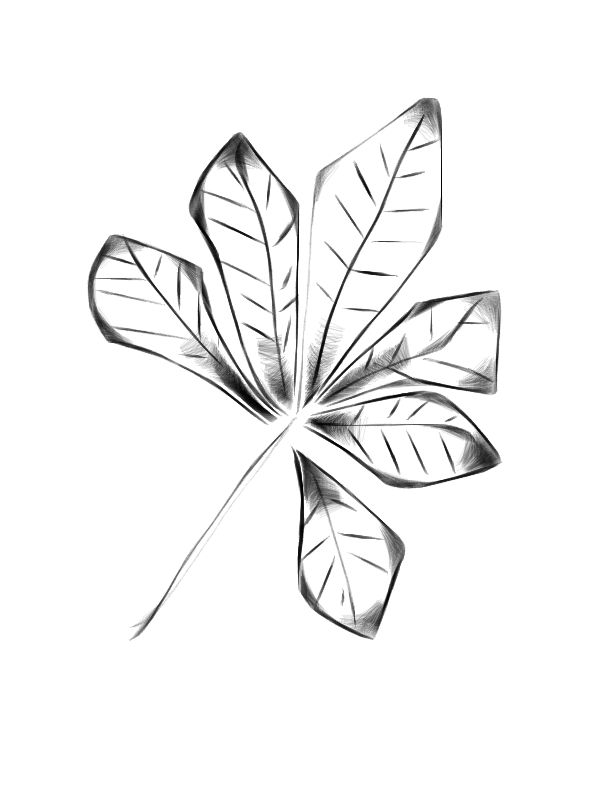
\includegraphics[width=0.50\textwidth]{cover/04.jpg}}

\title{Ересь о Киеве \\ \textsmaller[2]{редакция 11.0}}
\author{Петр Семилетов}
\date{19/20/2024}



\newcommand*{\plogo}{\fbox{$\mathcal{PL}$}} % Generic publisher logo

%----------------------------------------------------------------------------------------
%	TITLE PAGE
%----------------------------------------------------------------------------------------

\newcommand*{\titleAT}{\begingroup % Create the command for including the title page in the document
\newlength{\drop} % Command for generating a specific amount of whitespace
\drop=0.1\textheight % Define the command as 10% of the total text height

\rule{\textwidth}{1pt}\par % Thick horizontal line
\vspace{2pt}\vspace{-\baselineskip} % Whitespace between lines
\rule{\textwidth}{0.4pt}\par % Thin horizontal line

\vspace{\drop} % Whitespace between the top lines and title
\centering
\textcolor{Red}{
{\Huge ЕРЕСЬ О КИЕВЕ}\\[0.5\baselineskip] % Title line 1
%{\Large}\mbox{}\\[0.75\baselineskip] % Title line 2
%{\Huge четвертая редакция}} % Title line 3
}

\vspace{0.25\drop} 
\rule{0.3\textwidth}{0.4pt}\par 

\mbox{ }\\
редакция 11.0\\

\mbox{ }\\
Том 3\\


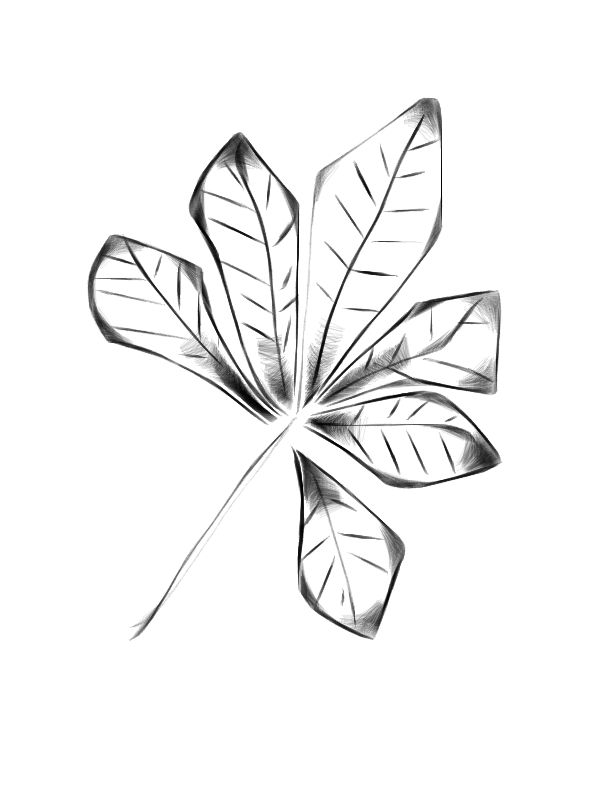
\includegraphics[width=0.40\textwidth]{cover/04.jpg}

\vspace{\drop} 

{\Large \textsc{Петр Семилетов}}\par 


\vfill
%{\large \textcolor{Red}{\plogo}}\\[0.5\baselineskip] % Publisher logo
{\large \textsc{Самиздат 2024}}\par % Publisher

\vspace*{\drop} 

\rule{\textwidth}{0.4pt}\par
\vspace{2pt}\vspace{-\baselineskip} 

\rule{\textwidth}{1pt}\par 

\endgroup}


\begin{document}

\pagestyle{empty}

\titleAT

\newpage

\pagestyle{plain}

\tableofcontents


\part{Игра в Городки}

\chapter{Легкость обретения Городка}

%Иногда второстепенное исследование, питаемое благодатным черноземом краеведения, разрастается до важного. Один за другой цепляются новые сведения, дело пухнет, как на дрожжах и уже не помещается в главу, что я хотел отвести под Городок.

Про Городище или Городок я давно и смутно знал, что есть такое на околице Троещины. Молва краеведов гласила, что тут при Литве жили Олельковичи\footnote{Род Олельковичей повёлся от Александра (Олелька) Владимировича, князя Слуцкого, которого литовский князь Казимир посадил править Киевом в 1443 году. В генеалогических работах считается, что род Олельковичей-Слуцких пресекся в 1593 году.}. Замок князя Симеона Олельковича! Романтический восторг.

Как в случае со Змиевой пещерой, я не подозревал, к каким открытиям приведет меня исследование этой местности, и какое направление придаст всей книге.

Однако прежде чем начать беседу о Городках обстоятельно, надо разобраться с водной системой левого берега, ее прошлым и настоящим. Левый берег всегда был у историков и киевоведов чем-то второстепенным, либо местностью, про которую можно выдумывать небылицы. 

Моя задача много скромнее, чем описание всех рек, ручьев и озер Левого берега. Мне нужна обоснованная документально модель водной системы, которую я могу использовать в рассуждениях о городищах. Построение такой модели подразумевает изучение взаимосвязи водоемов на протяжении столетий, основываясь на летописях, документах, картах, полевых наблюдениях и прочих источниках.

Я постараюсь дать обзор рек и озер киевского Левого берега, какими они были и какими стали, чтобы относительно свободно рассуждать о «городках». Коренные изменения, произошедшие со здешней водной системой, и отрывочные сведения об её прошлом делают задачу очень трудной. По возможности восстановленная картина течения рек и изменений местности послужит ключом к некоторым открытиям.

Перекроенный пуще правого, левый берег Киева меньше документирован историей. Находясь долгое время на окраине Черниговской губернии, он попадал на карты отрывочно и более известен по земельным документам, нежели в изображении. 

Редким подробным планом рек левого берега является загадочная карта землемера Сноевского, коей я посвящаю целую главу.

На вооружении у меня также отменный план «Участок р. Днепра у г. Киева» 1914 года и скудная старая его версия, 1910 года. Много пригодились советская карта 1943-го, того же года немецкие аэрофотоснимки, план РККА 1930-х и конечно же трехверстовки Шуберта середины 19 столетия.

Однако не всем картам я доверяю.

%, однако разжевать её помогает лишь план Сноевского, эдакий Розеттский камень, благодаря коему многое становится ясным – но как оно прояснилось для самого Сноевского?

\chapter{План Сноевского}

В 1912 году, в «Известиях Отделения русского языка и словесности Императорской Академии наук», томе XVII, книге 3, начиная со страницы 354, ученый-языковед Петр Лазаревич Маштаков опубликовал «План левого берега Днепра от устья реки Десны до устья реки Черторыи» землемера Сноевского, с приложением оного плана вклейкой.

Попади этот план в иную, нуждающуюся в таких знаниях среду, он пророс бы рядом новых исследований, стал одним из краеугольных источников и подспорьем в работе историков, археологов, краеведов. Этого не случилось.  Представляю обиду Маштакова, понимавшего значение предлагаемого им материала.

Публикацию плана Маштаков предварил словами:

\begin{quotation}
«План левого берега Днепра от устья реки Десны до устья реки Черторыи, с показанием селений, островов с озерами и речек луговых», составленный землемером Козелецкого повета Сноевским, хранится в I Отделении библиотеки Академии Наук. По-видимому, он составлен в ответ на запрос о топографии островов, расположенных, против г. Киева. Время его составления, судя по бумаге и почерку, можно отнести к первой половине прошлого столетия. 
\end{quotation}

\newpage

\begin{center}
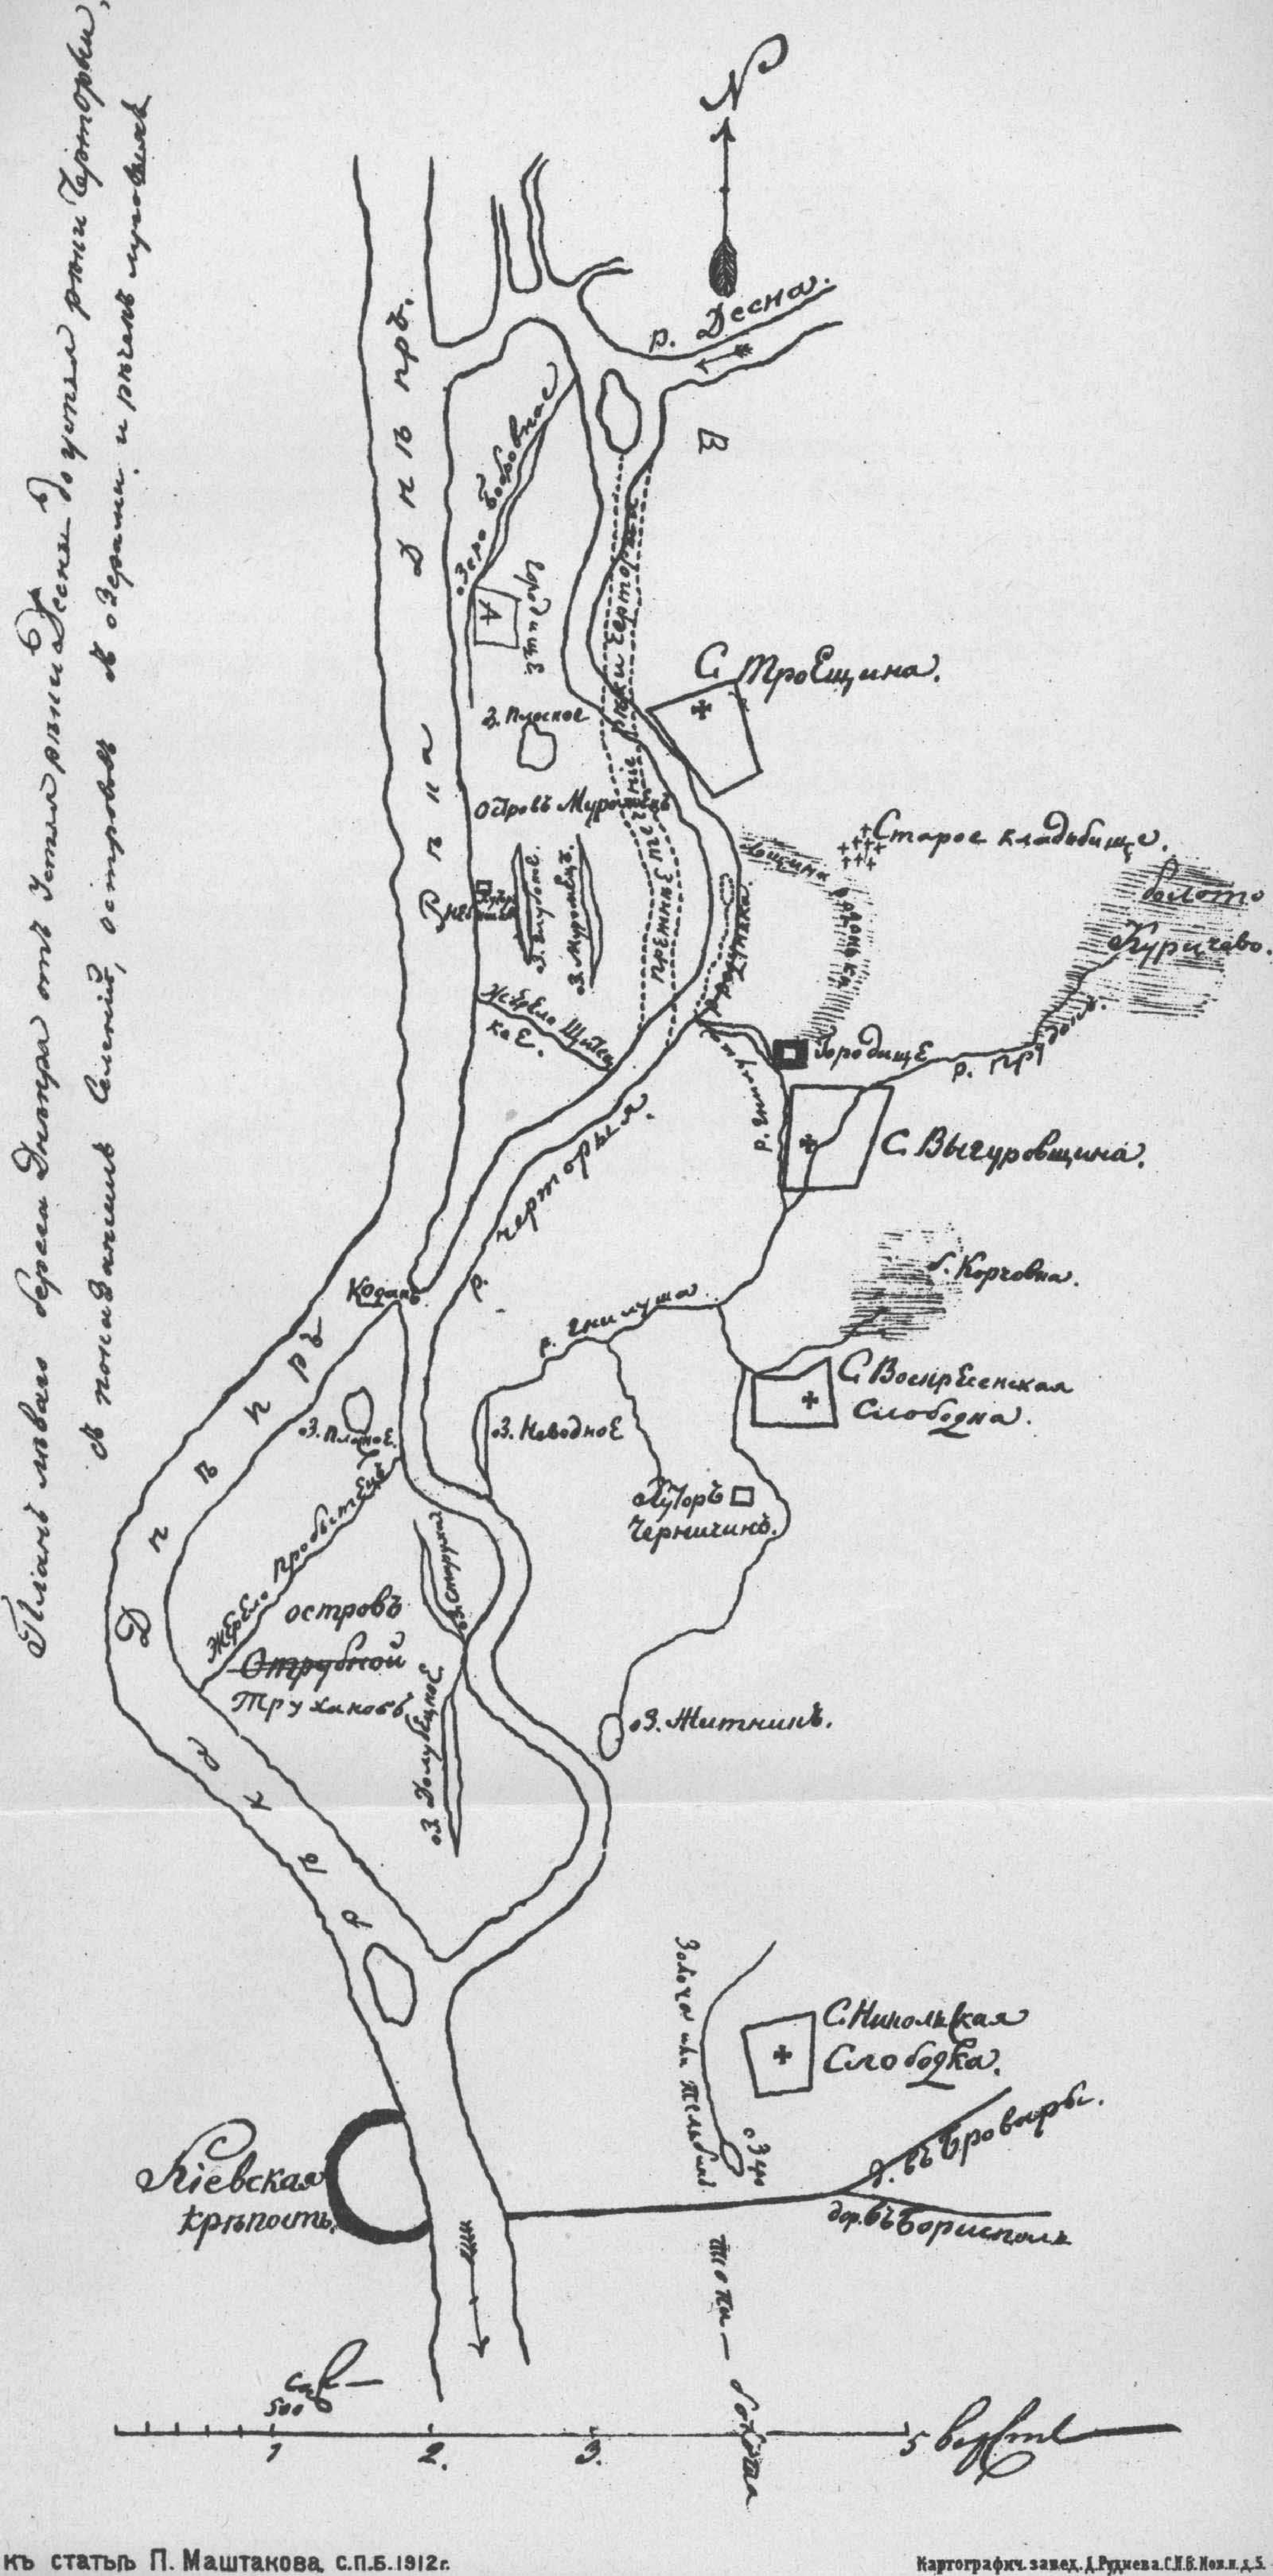
\includegraphics[width=0.82\linewidth]{chast-gorodki/snoev/356a.pdf}
\end{center}

\newpage

К плану прилагалось, от имени Сноевского, пояснение:
 
\begin{quotation}
По показанию старожилых поселян селений: Троещины, Выгуровщины, Воскресенской Слободки, и по распросу некоторых старожилых жителей города Киева, что остров, на котором находится хутор Небышев, название свое имеет по озеру, имеющемуся на нем, – Муромец, равно и тот хутор Небышев ныне называемой имел название по сему острову – Муромец; но когда сим островом владел для сенокосу Киевский комендант Небыш, то и хутор от тех пор таковое название себе получил. Другой же остров, отделяющийся проливом Кодаком, название свое имеет – Отрубной, и сии оба острова, по мнению старожилых людей, составляли в древности один остров Обрубной; ибо когда Черторыя подрезалась близко к Днепру, то бывшею там лощиной Кодаком называемую и прорезалась в Днепр, и старожилыя запомнят, что оной Кодак имел сначала весьма слабое и узкое течение; речька же Черторей в древния времена называлась Восковицей, которая против Троещина\footnote{С падежом всё верно – село тогда называлось Троещино.} имела свое течение, как означено на плане красными чертами\footnote{При публикации стало просто пунктиром.}, и которая быстротой воды, переменяя время от времени свое течение, врезала озерце и речьку Радонку, как на плане значит.

Лугу ж и ручья Ольгова никто из старожилых не знает, а полагают, что сие название лугу и ручья Ольгова от времени забыто, и называется ныне под каким-либо другим именем.

На подлинном подписано:

Повета Козелецкого землемер
Коллежский Ассессор Сноевский.
\end{quotation}

Я хочу обсудить карту и пояснение неотъемлемо с остальным текстом заметки Маштакова из публикации 1912 года.

Маштаков родился в села Кадышевке, Хвалынского уезда Саратовской губернии, в крестьянской семье, в 1872 году. Учил русскому языку в Смольном институте, был преподавателем в гимназии Л. Д.  Леонтьевской в Санкт-Петербурге и на общеобразовательных курсах А. С. Черняева. Получил чин коллежского советника. 

Среди печатных его работ – «Курс русского литературного языка» в трех частях, «К тексту Слова о полку Игореве», другие труды по языкознанию, в особенности по гидротопонимике – названиям рек. Большую часть его наследия уж трудно сыскать: «Список рек Днепровского бассейна» (1913), «Список рек бассейнов Днестра и Буга (Южного)» (1917), «Десна» (1918), «Список рек Донского бассейна» (1934), «Материалы для областного водного словаря» (1931). Умер ученый в феврале 1942 – блокадный Ленинград.

Но мёрзлая зима, когда голод заслонил холод, а дремота переходила в смерть, будет потом, а сейчас 1912 год, Маштаков в расцвете сил, воодушевленно сыплет мыслями о плане Сноевского, дополняя публикацию:

\begin{quotation}
Из «Плана» Сноевского мы можем почерпнуть новые данные для выяснения некоторых темных мест из области исторической географии, и этими данными подтверждаются изыскания П. В. Голубовского о местонахождении летописных оз. Долобского, реки Золотчи, Родуни («Историческая карта Черниговской губернии до 1300 года» в «Трудах XIII Археологического съезда в Екатеринославе 1905 года», т. II), а также и исследование В. Гошкевича о летописном Городце под Киевом («Замок князя Симеона Олельковича и летописный Городец под Киевом». Киев, 1890 г.). Теперь с еще большею уверенностью мы можем утверждать, что 1) село Радунь (Родунь, Радосынь), упоминаемое в Ипатьевской летописи под 1111 и 1151 годами и в Лаврентьевской летописи под 1146 годом, находилось между теперешними селами: Троещиной и Выгуровщиной, на реке Радуньке; 2) там, где на «Плане» находится Городище (рядом с селом Выгуровщиной), находился Городец, упоминаемый в Ипатьевской летописи под 1026, 1135 и 1180 годами, и, вероятно, он же и «Городок Песочный», с которого в 1238 году Менгукан, посланец Батыя, любовался Киевом; 3) Долобьское (Дулебское, Лубейское) оз. Ипатьевской летописи 1111 и 1151 гг. соответствует названному на «Плане» Долубецким; 4) река Золотча (Ипат. летописи под 1151 г.) вытекала из озера Золочи или Тельбень у села Никольской Слободы.

Кроме того на «Плане» Сноевского мы видим Гнилушу, Старое кладбище, озеро Бобровное, р. Прудок (Прудец), бол. Куричево, упоминаемые в актах Киевского Михайловского монастыря (В. Гошкевич, op. cit.); получаем впервые вариант названия для реки Черторыи – Восковица, и, наконец, по этому «Плану» можем восстановить несколько топографических названий, теперь уже утраченных: озеро Неводное, озеро Житник, болото Куричево, проток Кодак, жерело Щитецкое и др.

П. Л. Маштаков
\end{quotation}

Отмечу чрезвычайную осведомленность Маштакова относительно киевских левобережных водоемов и проявленный интерес к Городку.

Но вот Петр Лазаревич говорит про «село Радунь». Однако в летописях нет села Радунь. Есть \textit{название} Родунь. Когда Юрий Долгорукий (Гюрги) в 1151 году на лодьях плывет по Десне из своего Городка Остёрского и потом «сташа в Родуни», то можно заключить, что Родунь – по крайней мере залив Десны, где Гюрги хотел подождать конницу союзников – Половцев. К слову, в распрях 1151 года упомянуты два Городка – один возле Киева, а другой – Остёрский\footnote{В Остре, по улице Сеспеля, поныне есть на холме городище и Юрьева божница – остатки Михайловской церкви, входившей в состав крепости Юрия Долгорукого. Город Остёр же стоит на берегу реки Остёр, это приток Десны.}.

А в 1110 году Владимир Мономах «бяше в Радосыни», и в то же время с этой Радосынью летопись соотносит Городок, то есть Городок находился в Радосыни или около нее.

«Лубейское» вместо «Долобского» я нигде не встречал – неведомый источник Маштакова? 

Маштаков подтверждает планом Сноевского положение, что городище на плане и есть летописный Городец, но ведь на плане обозначено и другое городище – в северной части острова Муромца. Это второе городище (если верно мое сопоставление) в 1980-х заново открыл археолог Сагайдак, уроженец кстати села Троещины.

Датировка плана. Маштаков по бумаге и почерку относит его к первой половине 19 века. Я решил уточнить датировку. Самое простое было установить верхний рубеж, это 1877 год, ибо на плане село Троещина отмечено на Черторые, а не восточнее на материке, где отстроилось после указанного года. Далее, на карте есть Пробитец, а сей проток существовал еще в 1850 году. 

На давность плана указывает и то, что левый берег Киева отнесен к Козелецкому повету – а ведь известно, что позже он долго находился в другой административной единице, Остёрском уезде Черниговской губернии. Слово «повет» использовалось вместо «уезда», когда в 1781 году Малороссийская губерния была упразднена делением на наместничества, и Козелецкий повет вошел в состав Киевского наместничества. В последующих реформах «повет» по привычке был в ходу наряду с «уездом», потихоньку исчезая из обихода к концу 19 века. Сам же Козелецкий повет отошел затем к Черниговской губернии, а левый берег Киева – к ее же Остёрскому уезду, но гораздо проще датировать карту по ее составителю, землемеру Сноевскому!

Я напал на след Сноевского в документе «Ведомость о положении и пространстве города Козельца», опубликованном без даты в сборнике «Чернігівській губернії – 210 років. Збірник документів і матеріалів»\cite{cherndoc01}. В этом небольшом историко-краеведческом очерке есть отсылка ко временному промежутку с 1807 по 1811 год, как к «истекающему» четырехлетию. Следовательно, очерк сочинен между этими годами. Также указано, что городничим при составлении документа был Елинский, а землемером – коллежский асессор Сноевский. Козелецкий городничий Елинский упомянут еще в одном документе, 1810 года. Я не знаю, сколько лет Сноевский занимал должность землемера до и после 1810 года.

План Сноевского казался мне волшебным подарком судьбы, подтвердившим многие мои вычисления и догадки, сделанные на основании изучения имевшихся у меня тогда в малом количестве давних источников и частых вылазок на местность.

Я взял план на вооружение, но задался множеством вопросов.

Сначала на плане было написано «остров Отрубной», затем «Отрубной» похерено и поставлено «Труханов». В описании плана нет «Труханов». Значит, правку внесли в чистовик, той же рукой, но когда уже не было возможности исправить описание. В дошедших до нас документальных источниках «Обрубной» встречается раз, а «Труханов» – многократно. Да и слово «Труханов» сохранилось в живом предании до наших дней. Почему же землемер пишет крайне редкое название острова? И – Труханова ли?

План ориентирован примерно на север – тоже диковинка. Почти все планы Киева времени, приписанного плану Маштаковым, ориентированы на запад. Известное мне исключение – план «Положения местам вокруг Киева» 1753 года полковника де Боскета, тоже тороватый на водоемы, нигде больше не обозначенные.

Далее, почему отражены летописные названия, и они привязаны к более современным? Допустим, по источникам, Радунка встречается в литовско-польских земельных документах, но Золоча? Золоча в документах не упоминается.

Сноевский, чтобы сопоставить Тельбин с Золочей, должен был внимательно изучить по крайней мере Никонов список Повести временных лет, опубликованный в России в 1768 году, который, кроме Ипатьевского и Лаврентьевского (изданных позже), тоже подробно рассказывает о попытках Гюрги (Юрия Долгорукого) форсировать Днепр – по суше перетаскивали лодьи из Долобского озера в Золочу, а из Золочи выплыли в Днепр.

Напрашивалось два варианта. 

Первый – старожилы действительно помнили Тельбин как Золочу. 

Второй – землемер Козелецкого повета Сноевский был на короткой ноге с летописями, изучал их, сопоставлял былое с насущным. И не только с летописями. 

Общее впечатление от плана вообще такое, что над ним работал многознающий энтузиаст-краевед, пользовавшийся полевыми данными и, в гораздо большей степени – широчайшим набором документальных источников. 

Как я узнал позже, документ с упоминанием Восковицы, с показаниями местного рыбака Закгуры, относится к тому же архиву, с которым работал упомянутый Маштаковым Гошкевич. Сия бумага со времен Екатерины II хранилась в недрах Казенной палаты, пока митрополит Болховитинов не отыскал ее там купно с другими документами по землевладениям киевских монастырей 17-18 веков, и не передал оные документы в библиотеку Киевской Духовной Академии – а сделано это было до 1837 года. И в документе Черторыя вовсе не приравнивалась к Восковице. Но мы обсудим это позже.
  
Другие вопросы не давали мне покоя.

Почему Сноевский спрашивал (я тогда еще думал, что Сноевский лично общался с местным населением) у старожилов о луге и ручье Ольгином? Что за луг и ручей, где о нем еще говорится?

Почему на городище острова Муромца (около «озеро Бобровное») написана буква «А», а к северо-востоку от него, справа от начала Черторыи, поставлена буква «В»? Надо думать, существовала расшифровка этих букв, легенда карты. А много ли встречается карт – кроме тех, что помещены в археологические статьи – где отмечены городища?

Вчитаемся в название карты: «План левого берега Днепра от устья реки Десны до устья реки Черторыи». С какой целью Сноевский подробно картографировал именно этот участок? Юг на карте представлен слабо, но нехило – сопоставлением Тельбина с Золочей! Берлинский на такую смелость не пошел, он просто указал на некую левобережную цепь озер примерно напротив Неводницкой переправы. Мол, эти озёра – всё, что осталось от Золочи. А Сноевский указывает речку Тельбин как Золочу, но Тельбин протекает у него сам по себе, в то время как рядом были озера, во всяком случае знаменитое Свят\'ище.

Составителю плана понадобилось – точно как мне в этой книге – сложить картину левобережных рек на определенном отрезке, включая самые скудные притоки, но – в пределах протяженности Черторыи. Остальное составителю не нужно, но всё равно он проявляет глубокие познания, сопоставляя Тельбин с Золочей.

Таким образом план Сноевского, рассуждал я, заключает в себе тайну. Быть может, это часть какого-то исследования, затрагивающего городища, острова Муромец, Труханов, водную систему Черторыи и вероятно летописное село Ольжичи княгини Ольги. 

Причем Сноевский не просто отмечает современное ему положение объектов, но пытается проследить их изменение во времени – хотя казалось бы, зачем это, ежели, как полагал Маштаков, план «составлен в ответ на запрос о топографии островов»? И какое отношение к топографии островов имеют городища, представляющие чисто археологический интерес?

В начальном варианте этой части книги я основательно пользовался «планом Сноевского». Хотя почти сразу заподозрил, что составил его не Сноевский, но этим именем прикрылся некто очень сведущий в вопросе.

План в чем-то верен, в чем-то ошибочен, ибо, как я понимаю теперь, это итог большого, сложного исследования, включающего работу с архивом в том числе и тем, откуда черпал сведения Гошкевич. План отражает не местность в какое-то определенное время, но представление о местности, сложенное на основании документальных источников. 

В графическую основу «плана Сноевского» легла трехверстовка Шуберта середины 19 века, перерисованная лишь в общих чертах и небрежно. Обозначение урочищ на плане выдает знакомство не только с архивом документов 17-18 веков, но кажется принимались во внимание рассуждения из статьи Гошкевича.

Под воздействием размышлений над новыми для меня источниками я постепенно терял доверие к плану как к источнику, и наконец должен был весьма пересмотреть свое историческое видение местности, отринув многие из прежних рассуждений, основанных на плане.

Во время переделки глав я чувствовал обиду, но обида уравновесилась удовлетворением, ведь без пересмотра отношения к плану Сноевского я бы не выверил заново свои рассуждения и не пришел к более верному пониманию сетки левобережных рек, насколько это возможно исходя из наблюдений и документальных источников.

Далее я буду иногда обращаться к плану, однако не в качестве источника, а расценивая его как обобщение некоего исследования. К сожалению, выданного за источник.

Не буду разбирать, что на плане верно, а что ошибочно, оставляю вам сложить мнение самим, но предостерегаю от использования плана как путеводной звезды при толковании источников – звезда может завести не туда.

\chapter{Море Киян}

У меня в голове давно бродила шальная мысль, что возле Киева когда-то было море. Его упоминают и  старинные заклинания, что начинаются с убаюкивающей присказки – на море-окияне...

Когда я обратился к сборникам русских заклинаний и шептаний\footnote{В известных мне публикациях украинских заклинаний тоже встречается запев «на морі», но уже на «окіяні», остров Буян, дуб, но камень «білорізь».}, то обнаружил там более четкое название этого моря – в половине случаев говорится не «Окиян», а «Киян». На море на Кияне. Далее следует примерно такое – на острове на Буяне (Кургане)\footnote{Буян по корню сходно со словами «буево» – кладбище, «буйвище» – место прежнего кладбища. Вероятно и Буян означает нечто погребальное, вроде Могильного Острова. На это указывает и замена названия «Буяна» на «Курган».}, стоит бел-горюч камень Алатырь (Латырь). 

Алатырь или Латырь это янтарь. В некоторых – пермских краев – заговорах, вместо Алатырь так и говорится – Янтарь. Однако ведь янтарь желтоватый, верно? Но в старину белым обозначали чистое, светлое, прозрачное. Янтарь можно назвать и белым. Учтем, что значения названий основных цветов сейчас вообще трудно восстановить. Возможно, коричневый – от коры. Красный – красивый. Зеленый – наверное от слова «зело». А черный? Вот шоры лошадям на глаза надевали, но что значат эти «шоры» – тьму? А синий? А желтый? Желтый кстати смахивает на английское «gold». Если букву «g» читать как «ж», а не «г», то получится «жолд», что близко к «желтому».

Так вот об янтаре. На берегу нынешнего Киевского моря, около Межигорья, на холмах у поселка Новые Петровцы, попадается янтарь. Об этом упоминал еще в 19 веке Похилевич в своих «Сказаниях о населенных местностях»:

\begin{quotation}
село расположено на возвышенностях вокруг Межигорья; названо Новыми Петровцами в отличие от Старых, в 3-х верстах выше по Днепру лежащих. Основание Новых Петровец должно относить ко времени наибольшего процветания Межигорского монастыря, когда ему встретилась нужда иметь готовую прислугу под рукой, а не обращаться за ней в более или менее отдалённые свои имения. Грамоты королевские, в коих упоминается село Петровцы, относится к Старым Петровцам. [...]

%В настоящее время жителей обоего пола православных 1442, евреев 18. С 1859 года, как сказано выше, Петровцы отчислены из-под ведения фабрики, с предоставлением им входить в добровольные условия с содержателем её в случае снятия каких-либо фабричных работ. Жители также с успехом занимаются хлебопашеством, огородничеством и садоводством, но особенную их промышленность составляет выделка так называемого межигорского кирпича, известного своей огнеупорностью и твёрдостью, равняющейся твёрдости черепка. Он делается меньшего формата, нежели обыкновенный строительный и покупается на постройку печей. В Петровцах делают его до 500 000 штук ежегодно. 

Замечательно, что в горах петровецких попадается часто янтарь.
\end{quotation}

Испокон веков местное население торговало этим янтарем. Генерал-губернатору Бибикову в 1845 году докладывали: «Честь имею донести, что в Межигорье мальчики деревенские находят и продают янтарь целыми кусками». Искали его весной, в оврагах гор, когда оттуда большими обломками вымывались камни янтаря. Кроме как для продажи, он использовался в знахарских целях и для курения. Вот почему «горюч камень».

Был янтарь и в самом Киеве. В статье 1874 года «Исследование формации бурого угля Киевской губернии» Афанасий Рогович отмечает залежи янтаря около кирпичного завода Эйсмана (позже – Субботиной), а это у озера Глинки близ Лыбедской площади. Когда его берега еще не были застроены, я там лазал по обрыву, но ничего не нашел.

Хорошо, но ведь Киевское море – искусственное водохранилище. А как оно образовалось? Плотиной подняли уровень воды, вода заполнила впадину, потопив около трехсот селений. А впадина откуда? Неужели выкопали?

Нет, была издревле. Если перенестись в прошлое и представить, что в некоторое время уровень воды был выше, то получим точное подобие современного Киевского моря.

Оно кстати не такое уж глубокое. Мелководье – полтора метра, половина площади – три метра, есть под семь. Учтем наносы.

\begin{center}
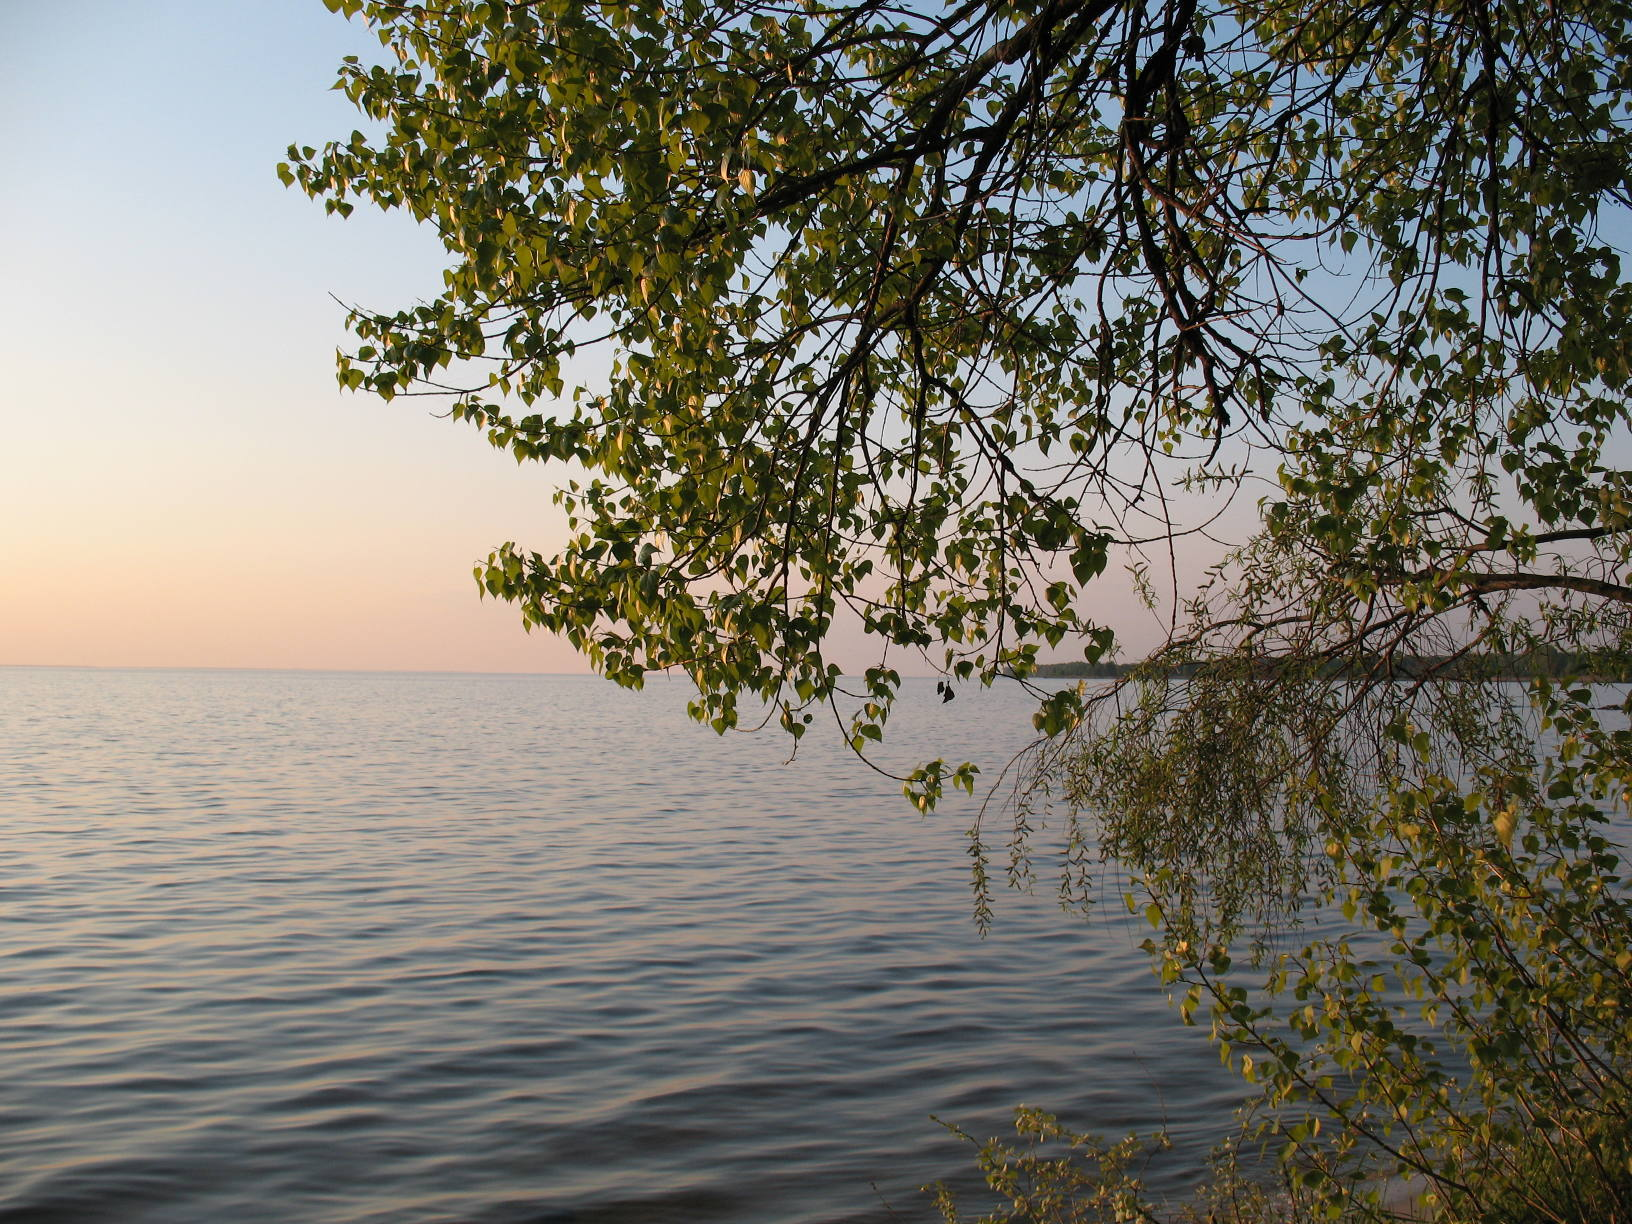
\includegraphics[width=\linewidth]{chast-gorodki/more/s_IMG_0577.jpg}

\textit{Киевское море, 2008 г. Фото Александра Бородина.}
\end{center}

А есть ли острова в этом море? Есть. Пауков\footnote{50°38'43"N 30°30'34"E}. Один из двух уцелевших на месте бывшего тут крупного (с Вышгород) поселка Сваромье, выглядит как плоский луг с лесом. А в северной части моря – Хильча близ дельты Тетерева, Волчьи горы\footnote{51°2'54"N 30°34'16"E}, Длинный, Майорский, Тятин, Прорезные острова, Бакланий и другие. Словом, в седую старину при повышенном уровне воды могло быть и море, и остров Буян или Курган на нем, где находили камень Алатырь – янтарь. Может, остров был священным, ибо заговоры толкуют про дуб на нем.% Не оттуда ли «перуновы дубы», что нашли в Днепре ниже устья Десны?

В первые годы после устроения Киевского водохранилища, площадь островов на нем была 21 км². Постепенно они размывались и остались только перечисленные.
 
В районе Киевского моря, в Днепр впадали и впадают крупнейшие его притоки – Припять, воды которой составляют 27 процентов общего стока Днепра, Десна – 20 процентов общего стока (устье Десны лежит южнее водохранилища на 4 км.), Тетерев – 13 процентов. Больше них только Сож в Белоруси (8,7 процентов), Сула (2,5), Псёл (3,6). Знаменитая Ворскла дает только 1,9 процента общего стока. По числам видно, что именно в районе теперешнего Киевского моря от притоков образуется основной сток Днепра. В море впадают и другие притоки – Ирпень, Козка, Смоловая.

Геологи и гидрологи утверждают, что в древности русло Днепра было гораздо шире. Инженер путей сообщений, архитектор и гидрограф Николай Иванович Максимович (1855-1928) пишет в своей до сих пор, с начала 20 века, непревзойденной монографии «Днепр и его бассейн»\cite{maxdnepr01}:

\begin{quotation}
Эта древняя долина Днепра имеет часто ширину в несколько раз большую, чем современная весенняя пойма реки. Так, для примера, если будем рассматривать на пространстве нескольких верст поперечные разрезы долины о. Днепр, в средней части его течения, под г. Киевом, то явно заметим, что рядом с границей современной весенней поймы поднимается на левом берегу вторая терраса древнего русла, распространяющаяся на далекое расстояние вглубь Черниговской губернии.
\end{quotation}

Нам обычно говорят, что эти поперечные разрезы относятся ко временам незапамятным. Так же, как геологические сведения о древнем море, покрывавшем некогда долину Днепра. Геологи считают, что суша и море несколько раз менялись местами\footnote{Например, под Каневом найдены кораллы и окаменевшие устрицы, в Волынской области – морские ежи, а в Киеве на кирпичном заводе Эйсмана-Субботиной (около озера Глинка) в 1887 году, в голубой глине – 17 зубов акулы!\cite{arhsved01}}. Но если это происходило в незапамятные времена, в чьей тогда памяти сохранились предания, что на левом берегу было море?

Боплан в 17 веке писал\cite{boplan01}:

\begin{quotation}
Утверждают, что в то время, когда древний Киев находился в апогее своего величия, морской пролив идущий мимо Константинополя\footnote{Имеется в виду Босфор.}, не был еще открыт. 

Есть предположение, осмелюсь даже сказать, точные доказательства тому, что равнины по другую (левую) сторону Борисфенеса, простирающиеся до самой Московии, были некогда сплошь покрыты водой; подтверждением чему служат якори, найденные несколько лет тому назад на реке Суле, в окрестностях Лохвицы, и некоторые другие указания. 

Кроме того, все города, которые расположены на этих равнинах, кажется, не особенно давнего происхождения и выстроены несколько сот лет тому назад.

Я поинтересовался сделать разысканья в истории руссов, чтобы узнать что-либо о древности поселений в этой стране, но тщетно. Я расспрашивал лучших из их ученых, от которых только и узнал, что большие и продолжительные войны, опустошавшие страну из конца в конец, не пощадили их библиотек, которые прежде всего предавались огню; что они припоминали старинное предание, по которому море покрывало никогда все эти равнины, как мы говорили об этом, и что это было приблизительно за 2000 лет до настоящего времени; что около 900 лет назад древний Киев был совершенно разрушен, за исключением двух храмов, о которых мы уже говорили раньше\footnote{София и Михайловский.}. 

Далее, в доказательство того, что море простиралось до Московии, приводят еще один весьма солидный довод, а именно, что все развалины старинных замков и древних городов, встречаемые в этих местах, всегда находятся на возвышенных местах и на самых высоких горах, и нет ни одного, расположенного на равнине. Это обстоятельство заставляет предполагать, что в древности равнина была затоплена.
\end{quotation}

Якоря на левом берегу, старинное предание, по которому море покрывало левый берег 2000 лет до Боплана... Так ли незапамятны времена, о которых говорят геологи?

К сообщению про якоря вплотную подходят строки Афанасия Шафонского, писанные в 18 веке в объемном, более 700 страниц труде про Черниговское наместничес\-тво\cite[стр. 6]{ochernignamest} – изданном почти сто лет спустя. Шафонский, рассуждая о реках и прочих водоемах, предполагает в древнее время более высокий уровень воды, мимоходом сообщая:

\begin{quotation}
[...] и поныне около Днепра, Десны, Остра и других в Днепр впадающих рек, по поемным местам и болотам\footnote{В сборнике «Этнографических материалы, собранные в Черниговской и соседних с ней губерниях» Гринченко\cite{grinetnochern} сообщает записанное Журавским предание о знаменитом болоте Замглай, по берегам которого в 19 веке находили якоря и сгнившие части «мелких судов». Замглай будто бы раньше был широкой, глубокой рекой. Современные ученые полагают Замглай заболоченной частью древней поймы Днепра. Опять же, выходит, не такой уж древней, раз крестьяне в 19 веке хранили память о судоходной реке Замглай, впадавшей то ли в Днепр, то ли в море.

Журавский описывает и «городки» по берегам болота – «возвышенные пространства, окруженные рвом и валом с одним или двумя выходами», которые еще на памяти стариков-рассказчиков служили прибежищем разбойникам. Их предводителей звали «телепнями». Телепень ставил на дороге булаву либо копье, как таможенный знак. Прохожий должен был уплатить дань, иначе у него отбирали всё.

Очевидно, что городки, построенные прежде шаек с телепнями, относились ко временам, когда Замглай в самом деле был рекой. Ведь нелепо строить крепости по берегу болота, ежели для этого существуют более удобные места.}, находят от больших, хотя не теперешних кораблей, но от морских и отличных судов куски, каковые теперь не только по малым, но ниже по самом Днепру не ходят.
\end{quotation}

Это значит, что Днепр не просто был глубок, но в него свободно проходили морские корабли с килем. Шафонский думал, что уровень воды упал, когда «греческие цари» прорыли Босфорский канал между Черным и Мраморным морями, а до того, мол, уровень воды был выше и она покрывала днепровские пороги, не препятствуя судоходству.

Итак, есть уже два варианта образования якобы сказочного моря-о-Кияна – в котловане по месту Киевского водохранилища, и просто на левом берегу, где по сей день множество огромных болот и озер. Русло столь широкое, что левый берег терялся из виду, тоже могло служить поводом, чтобы назвать его «морем» – что кстати можно видеть на дореволюционных фотографиях знаменитых «разливов на Днепре». На стыке 19-20 веков, ширина разлива Днепра у села Выгуровщины (нынешний жилмассив Троещина) составлял около 12 верст, выше Цепного Николаевского моста (теперь тут мост Метро) – 5-6 верст, а около моста – 3 версты.

И оба варианта не исключают один другой. А если предположить, что случился Всемирный потоп – после него море могло быть по всей Приднепровской низменности.

Большие озера у нас часто называют морями. Ладожское, Каспийское, Байкал. Даже в песне поется – «Славное море, священный Байкал». Так что большое озеро возле, а то и вдоль Киева могли называть морем, море-о-Киян, море Киян. Никто ведь не говорил раньше «киевляне», говорили «кияне», а на украинском по сей день так звучит. Чье море? Море Киян. Возле кого море, у кого? Море у Киян, море о Киян.

\vspace*{\fill}
\begin{center}
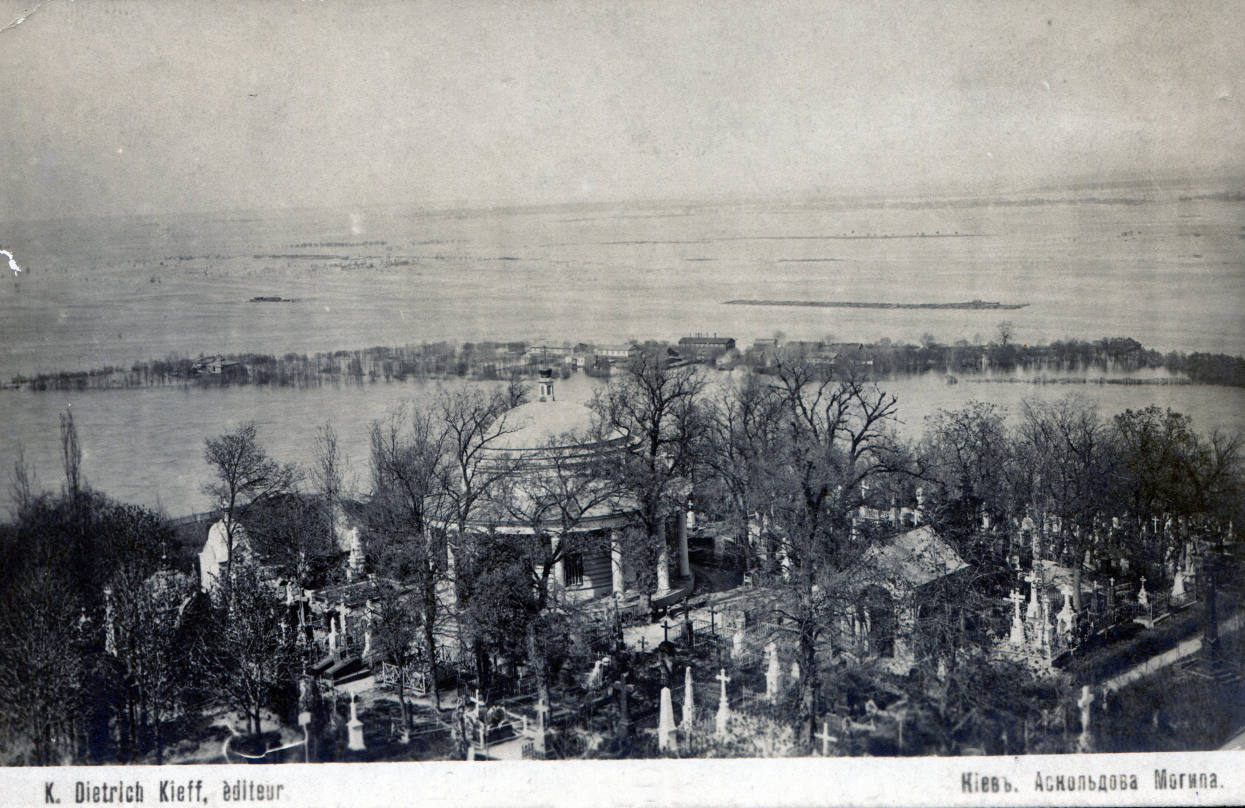
\includegraphics[width=\linewidth]{chast-gorodki/more/amogila1907.jpg}

\textit{1907 год, вид на левый берег с Аскольдовой могилы.}
\end{center}


В книге М. Возняка «Українські перекази»\cite{vozn01} есть невесть откуда переписанное предание о море на Киевщине и Полтавщине, и дескать, приплывавшие кораблями купцы платили киевскому князю десятину, за которую и построили Десятинную церковь. А когда святой Андрей водрузил на здешней горе крест, то море иссякло, но часть его спряталась под горой, и не зря когда Андреевскую церковь строили, то в склоне открылся родник, и чтобы с ним бороться, покупают смолу тряпки. Вот почему на этом храме нет колокола. Чуть ударит, пробьет вода и зальет окрестности. 

Давно залита водой история Киевщины, история всей древней земли вдоль Днепра. Водохранилища навсегда похоронили под собой курганы и давние поселения, затопили луга, уничтожили малые реки, озера, заболотили берега. Горе дому человеческому, горе звериной норе!

Только под Киевским водохранилищем навсегда скрылись селения с именами, от коих веяло стариной – Сорокошичи, Сваромье, восточная часть Козаровичей, Чернин. Иные, где ныне суша по берегам, обезлюдели и стерлись – Теремцы, Новый и Старый Глыбов, Сивки.

А остальные искусственные моря? Гидроэлектростанции дали энергию, платой за нее стала, пожалуй б\'ольшую часть левобережья древнейшего очага цивилизации. Правый же берег неистово пожрали кирпичные заводы да загадили мусорные свалки.

\chapter{Черторыя}

Она – одна из главных героинь в этой части. Надо познакомиться с Черторыей ближе, иначе ничего нельзя будет понять потом, ни про речку Радунку, ни про городища.

Однако я изменю своему правилу и сделаю несколько важнейших утверждений, не подводя к этому источниками. Доводы изложу позже. Мне нужно быстро, не отвлекаясь, начертать вехи развития Черторыи.

Но прежде кратко изложу популярные знания на 21 век.

Привыкли считать, что левый берег Киева это берег Днепра, а ведь на деле это берег Десёнки и Черторыи, Чертороя. 

На многих картах и в быту Десенка с Черторыей не различаются, ими называют одно и то же русло, что начинается из Десны и на тринадцать километров вдоль левобережья тянется к югу параллельно Днепру, отделенное от него большими островами – Муромцем, да Трухановым с Долобским.

Дачники Русановских садов называют свою речку Десёнкой. На трехверстовой карте Шуберта 1863 года издания, б\'ольшая часть 13-километрового русла подписано «Черторыей», однако до широты троещинской улицы Марины Цветаевой его верховье обозначено как «Старая Десна», что подразумевает – там протекала Десна издревле. На одном плане 1896 года Десной подписано русло Черторыи от Десны до Труханова острова.

На плане Шуберта, 13-километровое русло смыкается с Днепром в двух местах. Северное – пролив Пробитец, между нынешними мостами железнодорожным Петровским и Московским. Теперь там суша – перешеек от Труханова острова к острову Муромцу, выезд с Труханова к Московскому мосту. И южное впадение у моста Метро, через пролив между островами Труханов и Гидропарк.

На некоторых картах Десенка – русло от Десны до бывшего Пробитца, а южнее идет уже Черторыя.

Как же правильно называть эту реку – Черторыя или Десенка, либо это два разных водоема, что соединились?

Вопрос поставлен ошибочно. Ответ будет дан другой, очень неудобный.

Современная Черторыя – русло, поглотившее части других, давних русел. На протяжении веков оно своеобразно развивалось, ползя на север и юг и влияя на смежные водоемы, пока на севере не достигло Десны, а на юге Гидропарка. Рассмотрим, двигаясь по времени от прошлого к настоящему, изменения Черторыи.

\textbf{Итак, утверждение первое} – Черторыя поначалу, как она возникает в летописных упоминаниях, это водоем около Труханова острова, однако не севернее.

Слово «черторыя» или «черторой», по словарю Даля, означает «овраг, рытвина от воды». На карте Украины раскидано много Черторый. Даль знал также пролив «Пробитец, под Киевом, соединяет Черторою с Днепром».

В летописях, по времени сообщения, Черторыя впервые появляется в Воскресенском и Никановском списках, а это списки новые, 16 века. Сведения относятся ко времени Гюрги – Юрия Долгорукого.

Вот что сообщает Никановская летопись, за 6658 год (1150):

\begin{quotation}
а князь Юрий Долгорукий Владимерич Маномашь в то же время приде к Киеву з Давыдовичи и Олговичи, и ста у Черторьи\footnote{Воскресенская летопись: «ста у Черторыи».}, и посла за Изяславом Мстиславичем князя Святослава Всеволодича и сына своего князя Бориса, и гнаша по нем до Чертова леса, и не достигше воротишася вспять 
\end{quotation}

Старинная Ипатьевская летопись излагает то же иначе – делаю сокращения, выпуская всё не касающееся вопроса:

\begin{quotation}
И в то веремя приде Гюрги с сынми своми, и Володимир, Изяслав Давыдовича, и Олгович Святослав, и сыновец его Святослав Всеволодич, над берег противу Киеву.

Кияне же мнози поехаша в насадех к Гюргеви, а друзии почаша в насадех дружину его перевозити на сю сторону в Подолье.

Вячеслав же с Изяславом рекоста видивша то: «на нею веремя ныне есть». [...]

В втрий же день приде Володимер Галичьской к Олгове могыле, тако же и Дюрги приеха к нему [...] и ту ся целоваша не съседаюче с коний, у Сетомля на болоньи; сдумавше послаша по Изяславе Святослава Всеволодича, Бориса Дюргивича. и гониша но них до Чертова леса, и не постигше их, взвратишася.
\end{quotation}

Что же, здесь нет Черторыи, сказано просто «над берег противу Киеву». И – мы разберем это далее – в описании попыток Гюрги захватить Киев, Ипатьевская летопись не упоминает Черторыю среди прочих урочищ.

Я полагаю, что Никоновский и Воскресенский список напрасно уточняют «ста у Черторыи» – ее тогда, для времени описываемых событий, просто не существовало. А в 16 веке – несомненно, уже была. Да и гораздо раньше.

Та же Ипатьевская летопись за 6688 (1180):

\begin{quotation}
Святослав въеха с братома  Киев. Половци же испросиша у Святослава Игоря, ать ляжет с ними по Долобьску, Святослав же отпусти.

[...]

Половци же бегаючи перед Русью потопоша мнозе в Черторыи, а инех изимаша, а другыя иссекоша.

[...]

Игорь же виде Половце побежены, и тако с Концаком вскочивша в лодью, бежа на Городец к Чернигову.\end{quotation}

Половцы с Игорем расположились по Долобську (из летописи нельзя понять, местность это или водоем), затем воины, состоящие из Руси, начали их громить и Половцы тонули в Черторыи. Игорь, однако, где-то там вскочил в лодью и умотал в Городец к Чернигову (это другой, не киевский Городец). Значит, тогда был некий водный путь от Долобська к Десне.

По этим летописным сведениям мы можем только и понять про близость Долобська и Черторыи, да что Черторыя была водоемом достаточным для утопления Половцев. %Возможно, еще в летописные времена Черторыей стали называть рукав Днепра около Труханова острова, но прямых указаний на это в источниках нет.

\textbf{Утверждение второе} – на 16 век, Черторыя это водоем южнее Воскресенки, всё еще на уровне Труханова острова.

\textbf{Третье} – на 17 век, в Черторыю севернее Труханова острова и Московского моста (где нынешний остров Муромец) пробивается рукав Днепра. Таким образом протяженность Черторыи увеличивается на север. Однако, Черторыя еще не соединена своим устьем с Десной. Покамест устьем Черторыи можно считать этот рукав Днепра.

Дальнейшие века.

1. В Черторыю с севера пробивается Десна, а рукав Днепра (по нынешнему острову Муромцу) пересыхает, «отпадает». Устьем Черторыи становится Десна.

2. Днепр снова пробивается в Черторыю уже на широтах Московского и Петровского мостов – так возникает пролив Пробитец, а ниже его русло Черторыи раздувается.

Таковы важнейшие вехи развития Черторыи.

Название же Десенка рождается, кажется, в 19 веке, для обозначения русла Черторыи от широты Пробитца до устья у Десны. Термин «Десенка» широко используется в гидрологических текстах стыка 19-20 веков, где Десенкой считают рукав Десны, а Черторыей – рукав Днепра, и Десенка впадает в Черторыю. Таковы были представления, например, известного инженера, гидролога Николая Максимовича. В этой книге я применяю название Черторыя ко всему современному руслу от Десны до Гидропарка, и к руслу меньшей протяженности в давнее время, о чем буду говорить особо.

Максим Берлинский в 1820 году написал\cite{berl01} про Черторыю и Пробитец, тогдашнее их значение:

\begin{quotation}
Черторыя.

Речный судопроходный рукав, отделяющийся от Десны близ устья ея, протекающий по луговой стороне против Киева, и наконец сливающийся с Днепром против самаго Николаевского монастыря\footnote{То есть на уровне Дворца Пионеров и Аскольдовки.}, из стари и теперь называется Черторыею.

На средине своего течения соединяется она также с Днепром  посредством течения пролива, называемого Пробитцем. Сей Пробитец учинился с 1777 года от напору реки, когда предприняли было каменною гатью на Днепре отворотить его стремление от Киева-Подола в Черторыю.

Теперь сим Пробитцем проходят суда в глубокую Черторыю, избегая многих непостоянных отмелей, бывающих у Киева на Днепре.
\end{quotation}

Иными словами, вместо плавания от Подола сразу вниз по Днепру вдоль правого берега, поднимались по течению чуть выше, зачем через Пробитец шли в Черторыю и ею спускались в Днепр же на широту немногим севернее нынешнего моста Метро. А прежде того, в 1777 пытались отвести воды Днепра в Черторыю при помощи каменной гати, дабы Днепр не заливал в половодье Подол.

И. Ф. Тимковский в сочинении «Мое определение в службу. Сказание в 3-х частях. Писано в 1850 г.» сообщал:

\begin{quotation}
и как Днепр, отбиваемый устьем Десны, всякий год весною на Подоле к Оболонью разом обширно заливал и вырывал берег, и мы видели тогда плывущими на нем избы, сараи, обломки: то в 1788 году, для отвода его, разрывали у левого берега рукав, Черторый, поденной платою вольноприходящим от голову до 3 коп. Теперь слышно, что полагают запереть Черторый, для обмелевшего Днепра.
\end{quotation}

В 1840-50 годах Черторыю в районе между современными Московским и Петровским мостами, наоборот, отделили от Днепра запрудой, чтобы из Днепра вода не уходила налево. А запруда из Десны в Десенку впервые была построена в 1884-м, после чего в Десенку стало уходить меньше воды.

%Гидролог, инженер Максимович писал, что в конце 18 века в истоке Черторыи (у Десны) сделали запруду, затопив там байдаки с камнями, чтобы вода шла дальше по Десне через ее устье и питала обмелевший Днепр. Теперь в истоке Четорыи – тоже дамба и первый водозабор Деснянской водопроводной станции.

\begin{center}
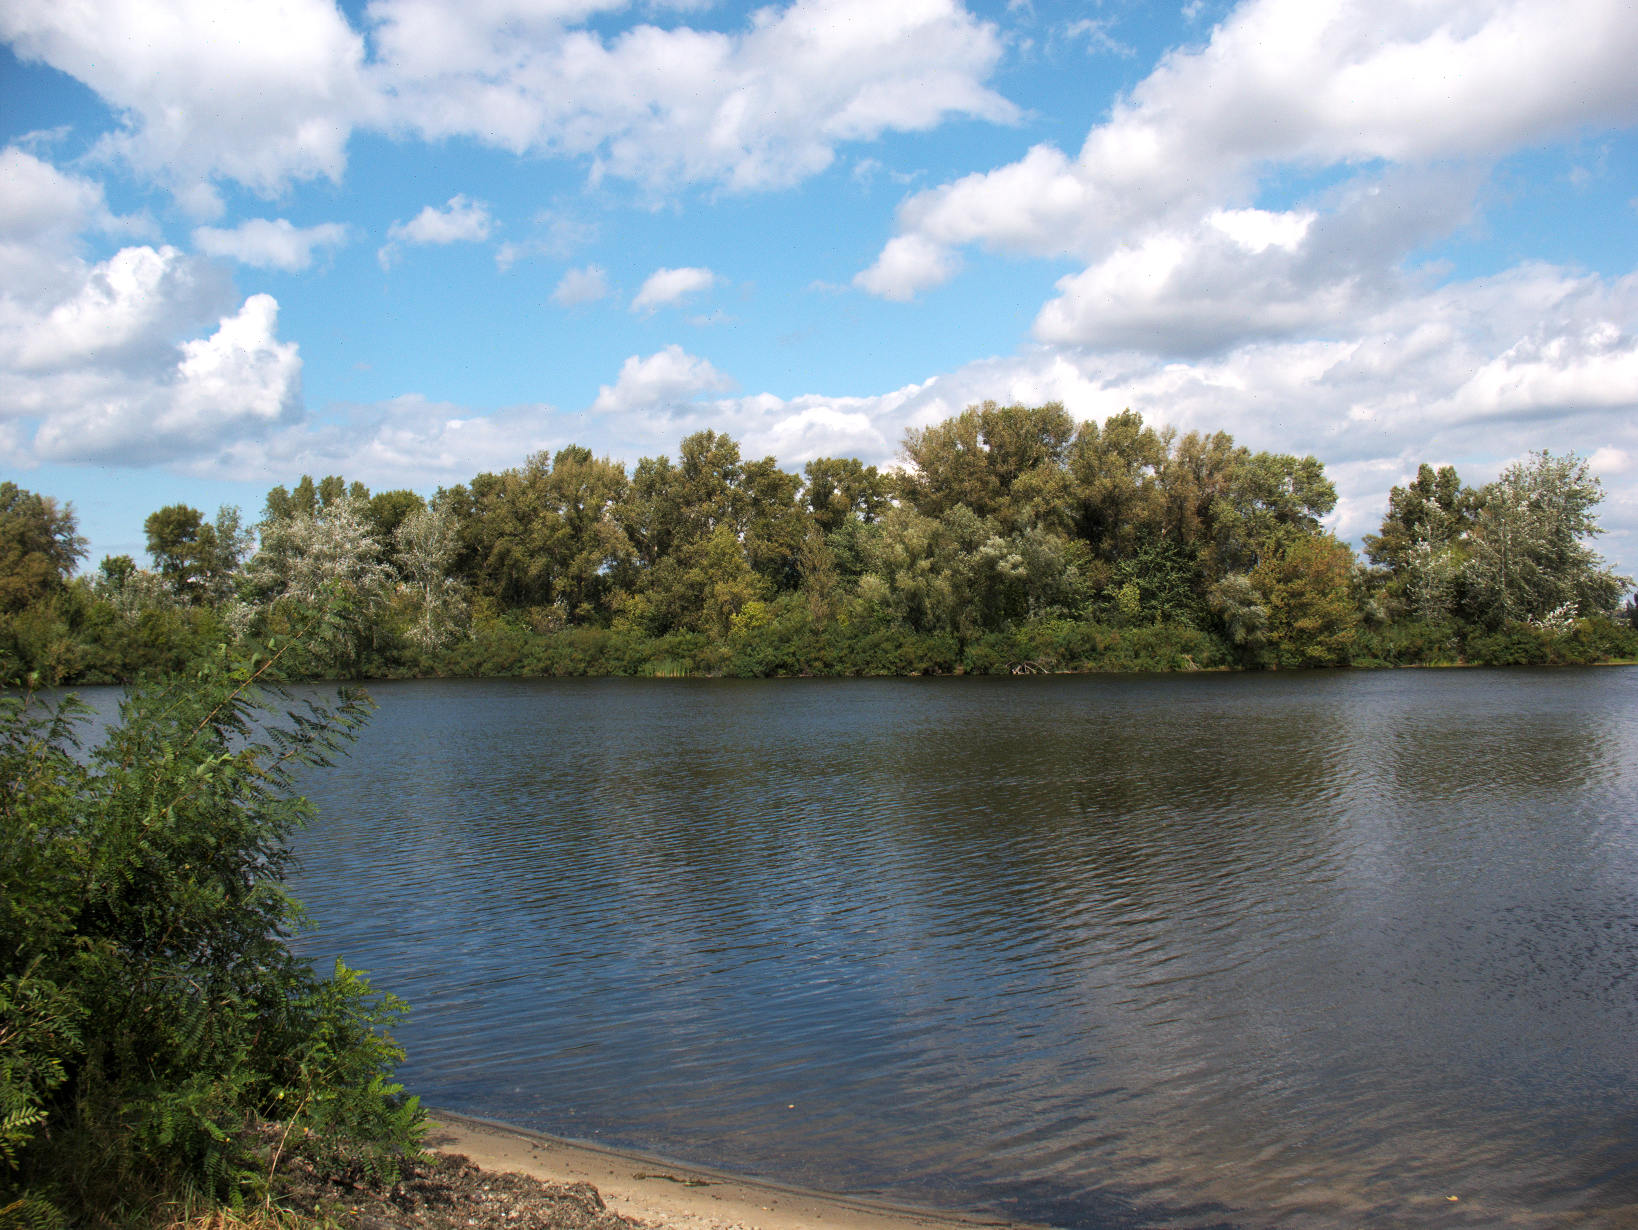
\includegraphics[width=\linewidth]{chast-gorodki/cherto/s_mur_CRW_3927.jpg}

\textit{Заводь Черторыи на острове Муромце. 2014 год.}
\end{center}
 
Современная Черторыя принимает в себя все левобережные воды на протяжении от Десны до моста Патона. Течение в Черторые быстрее, нежели в Днепре, глубина порядочная – на разных участках фарватера от 15 до 9 метров, конечно есть и мельче. При сопоставлении с Днепром можно сказать, что Черторыя на одних с ним широтах течения обычно чуть глубже, однако немного \'уже. Например, в районе Московского моста, с южной его стороны, глубина фарватера Черторыи равна 8 метрам, а Днепра – только 6 метров. У Труханова острова напротив Подола, фарватер Днепра – 7-9 метров, а по другую сторону Труханова, Черторыя дает 9-14 метров.

Я даже не говорю о чудовищных заливах к югу и северу от проспекта генерала Ватутина – дно их это ямы до 20 метров глубиной, образовавшиеся от добычи песка. В середине 20 века здесь был большой остров в Черторые, отрезанный с востока от материка озером Неводным, давним остатком того русла Черторыи, когда в него не вливался еще Днепр около Петровского моста. От острова сохранился участок между Московским мостом и перекрестком улицы Бальзака с проспекта Ватутина. Нижний залив известен ныне как «залив Десенка».

А на дикой местности непосредственно к северо-запа\-ду от перекрестка, был и остается водоем с рыжей водой\footnote{Исток: 50°30'17"N  30°34'38"E, устье: 50°30'2"N 30°34'8"E.}, про него я поведаю позже, ибо разговор будет долгим.

В 19 и по середину 20 века, от Десны на юг примерно до Петровского железнодорожного моста, русло Десенки было, в отличие от теперешнего, довольно узким, ну – чуть шире проспекта Генерала Ватутина. А вот дальше вниз – как придется, местами почти с Днепр. Почему так? Да потому, что южнее моста в Черторыю грубо вторгся Днепр, и русло первой одно время несло в себе воды и Днепра, сомкнувшись с ним Пробитцем в точке между островами Муромцем и Трухановым.

За столетия существования и развития, Черторыя отобрала поглотила много водоемов, отрезала от материка несколько островов и со временем дошла до нынешнего моста Патона. Когда там находилось устье Черторыи, Гидропарк был островом. А до конца 19 века превратился в полуостров, продырявленный озерами и остатками прежнего русла Черторыи. Её – на уровне Николаевского моста и позже выстроенного почти на его месте моста Метро – Днепровской дамбой свернули на запад к Днепру. 

Через Днепр, от острова до Киева, в 1850-х по проекту Чарлза Виньоля построили Николаевский цепной мост. Основу его составили пять кирпичных опор, или «быков», пролеты между ними поддерживались цепями, закрепленными в арках. Цепи были из двухсоткилограммовых звеньев, каждое длиной в 3,6 метра. На правом берегу у моста соорудили пятикупольную часовню святого Николая, и с Печерска подвели Николаевский спуск, именем связанный с издавна стоявшим выше, на горе, Никольским Пустынным монастырем и церковью святого Николая на Аскольдовой могиле.

\begin{center}
\includegraphics[width=\linewidth]{chast-gorodki/cherto/\myimgprefix nikmost01.jpg}

\textit{Николаевский цепной мост и Предмостная слободка.}
\end{center}

Красавец-мост, архитектурное чудо, ставшее одной из знаковых частей города, прослужил людям около семидесяти лет. А 10 июня 1920 года из Киева драпали польские войска, чей командующий, Эдвард Рыдз-Смиглы, приказал уничтожить мост. Для этого понадобилось немного – по заряду взрывчатки на каждую несущую цепь. Пролеты упали в воду. Там их вместе с цепями взорвали год спустя уже наши, чтобы суда могли плавать.

На следующей фотографии, 1920 года, хорошо видно эти ослабленные цепи, и юго-восточную часть Предмостной слободки с церковью Иоанна Рыльского, справа. А дальше, по Броварскому шоссе выглядывает Николаевская церковь\footnote{Снесена в 1961 году при проложении линии метро. Краеведы любят рассказывать, что в ней венчались Гумилев с Ахматовой.} – это уже через Русановский пролив (теперь он – от моста Метро и до Патона, вдоль Русановки), в Никольской слободке! Церковь Иоанна Рыльского была возведена в 1909 году на средства Варвары Бобриковой, 20500 рублей, в память о погибшем на войне муже Иване. Закрыта в 1935-м с передачей здания под общежитие рабочим, что строили школу. Сгорела в 1943 году вместе со Слободкой.

\vspace*{\fill}
\begin{center}
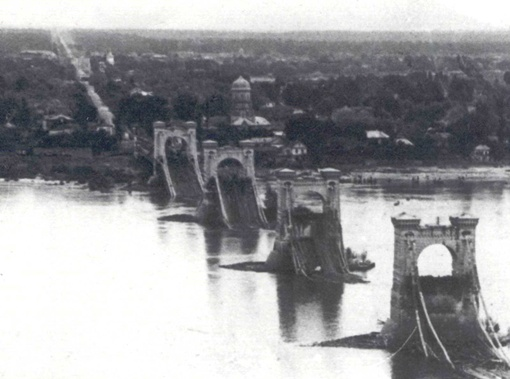
\includegraphics[width=\linewidth]{chast-gorodki/cherto/1920-cep.jpg}
\end{center}
\vspace*{\fill}
\newpage

Руки, а главное – голова – до восстановления моста через Днепр дошли только в 1925-м. Евгений Патон, надстроив опоры старого моста, поставил сверху новый, на него очень похож современный Пешеходный. Мосту присвоили имя Евгении Бош, которая застрелилась в том же году. Бош – профессиональный революционный деятель из тех, кто в мирное время не расстается с маузером. Мать двоих детей, она не научилась ценить ни чужие жизни, ни свою.

19 сентября 1941 года наши войска при отступлении уничтожили за собой мосты – взорвали железнодорожный мост имени Петровского, мост Евгении Бош, южный Дарницкий, да спалили, облив смолой и бензином, деревянный Наводницкий мост. Живучие опоры Николаевского моста и после войны торчали из воды, пока рядом не построили мост Метро.

Прежние опоры видны в старых фильмах, например в комедии «Она вас любит» с Вицыным, где он играет роль ветеринара зоопарка. В 1960-х опоры взорвали, уцелевшие остатки трех ныне затоплены, ведь после запуска Киевской и Каневской ГЭС уровень воды в Днепре у Киева поднялся. Но когда река сильно мелеет, опоры заметны, как было весной 2010 года.

После сооружения Николаевского моста, на будущем Гидропарке стали селиться рабочие с правого берега и возникла Предмостная, или Ближняя Никольская слободка, она же Печерская.

В Гидропарке Николаевский мост не был первым. Раньше на его месте уже существовала переправа, наводили плавучий Спасский мост\footnote{По имени очень крутого Спасского спуска, а тот назван от близости к церкви Спаса на Берестове, что стоит выше на горе. О перевозе через Днепр по сему месту сказано еще в книге «Тератургиме» лаврского ученого монаха Афанасия Кальнофойского, в 1638 году.}, а другой был южнее около удолья Наводничей (между ними и Лаврой), и на левом берегу подходил к старинной дороге в Дарницу, у Резановского трактира с постоялым двором. По крайней мере с середины 18 века, за сим мостом, по левому берегу на север шла дорога к Никольской слободке, сворачивая затем на восток к Москве.

Давний путь, известный ныне под именем Броварского шоссе, прежде раздваивался. Одна ветвь соединялась с ним от Наводницкой переправы, другая – от Спасского моста. Последняя существовала уже в 1830-х. Сразу за Спасским мостом начиналась дорога, по деревянному мосту переваливала через Русановский пролив – нижнюю часть Черторыи, и материком направлялась к Никольской слободке (Левобережка) и дальше.

В начале 20 века деревянный Русановский мост заменили металлическим двухпролетным, по проекту Николая Аполлоновича Белелюбского, а также инженера Григория Кривошеина и архитектора Владимира Апышкова.

По нынешней линии метро в Гидропарке и Русановскому мосту была устроена Днепровская дамба. Вот Гидропарк конца 19 века в «разрезе», с севера на юг (из «Пояснительной записки к проекту окончания выправительных работ на р. Днепре у г. Киева», Николая Максимовича, изданной в 1896 году). Показаны, кроме прочего, два засыпанных моста.

\begin{center}
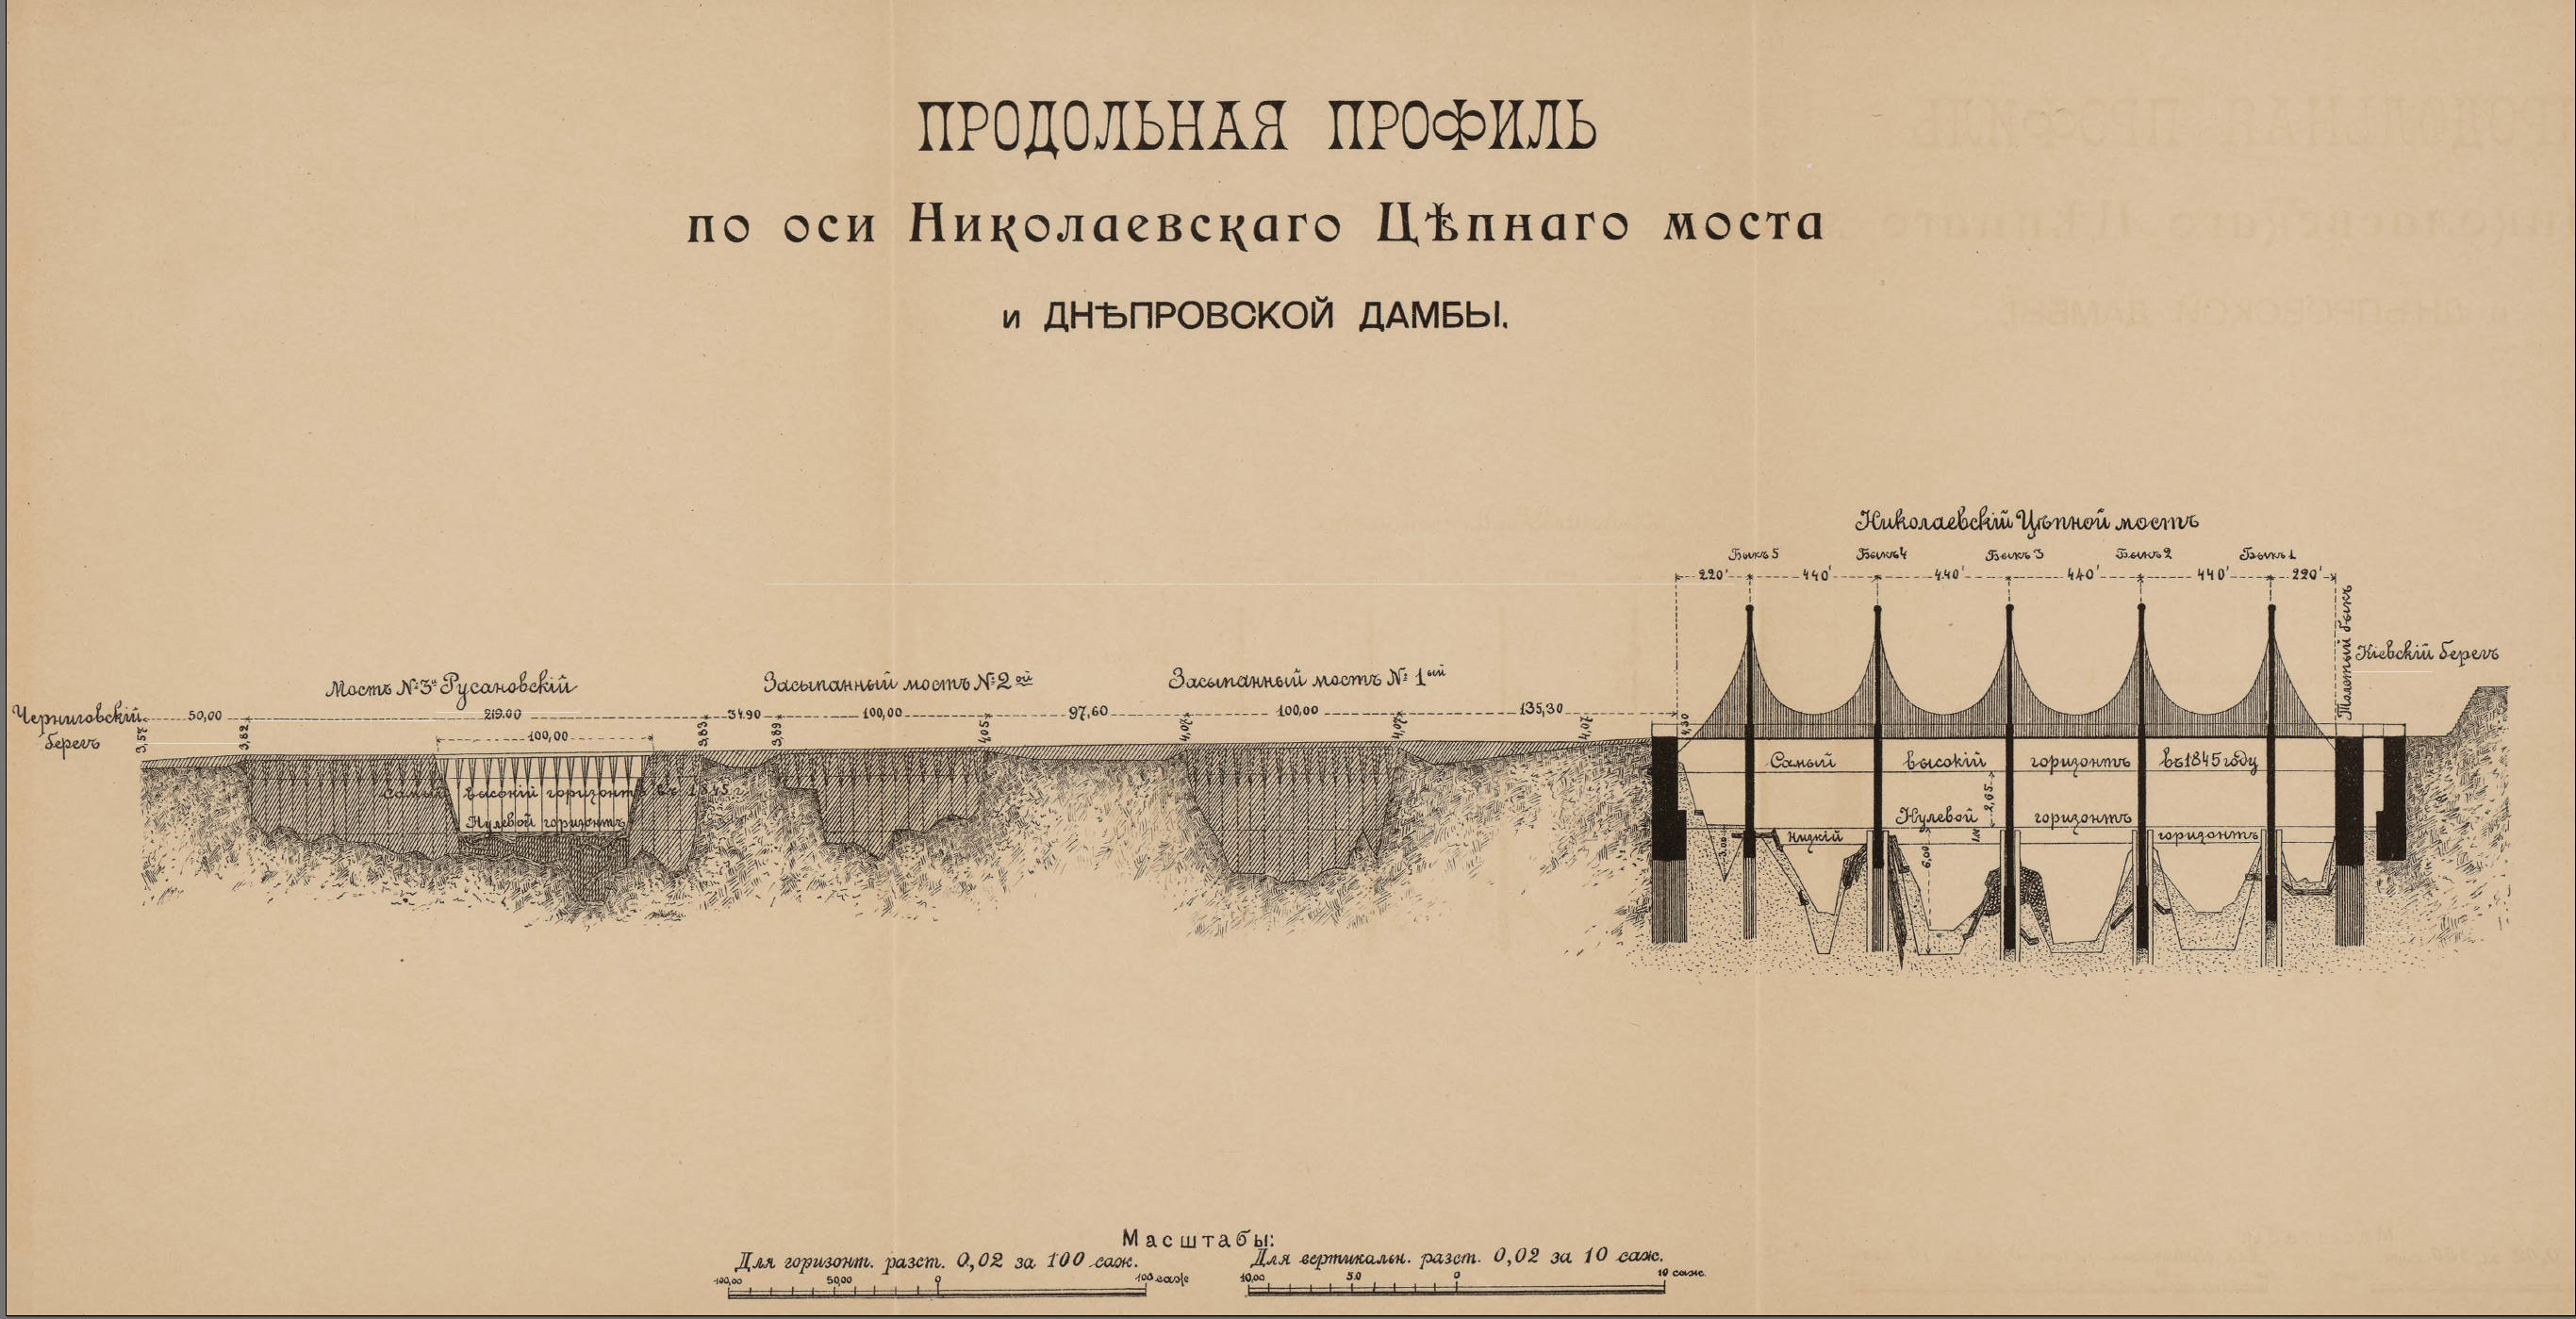
\includegraphics[width=\linewidth]{chast-gorodki/cherto/1896-profil.jpg}
\end{center}

В 1912 году в Дарницу (там где сейчас Дарницкий вокзал) через оба моста, Николаевский и Русановский, проложили линию мото-трамвая от Почтовой площади до железнодорожной станции «Дарница». Билет туда из Киева стоил 20 копеек\footnote{В больших городах, средняя зарплата рабочего составляла тогда около 22 рублей. Чернорабочий получал 120 копеек в день, токарь – 250. Кочан капусты стоил около 18 копеек, десяток яиц – 30 копеек, фунт ржаного хлеба – 3 копейки.}, трамвай ходил раз в 20 минут.

\begin{center}
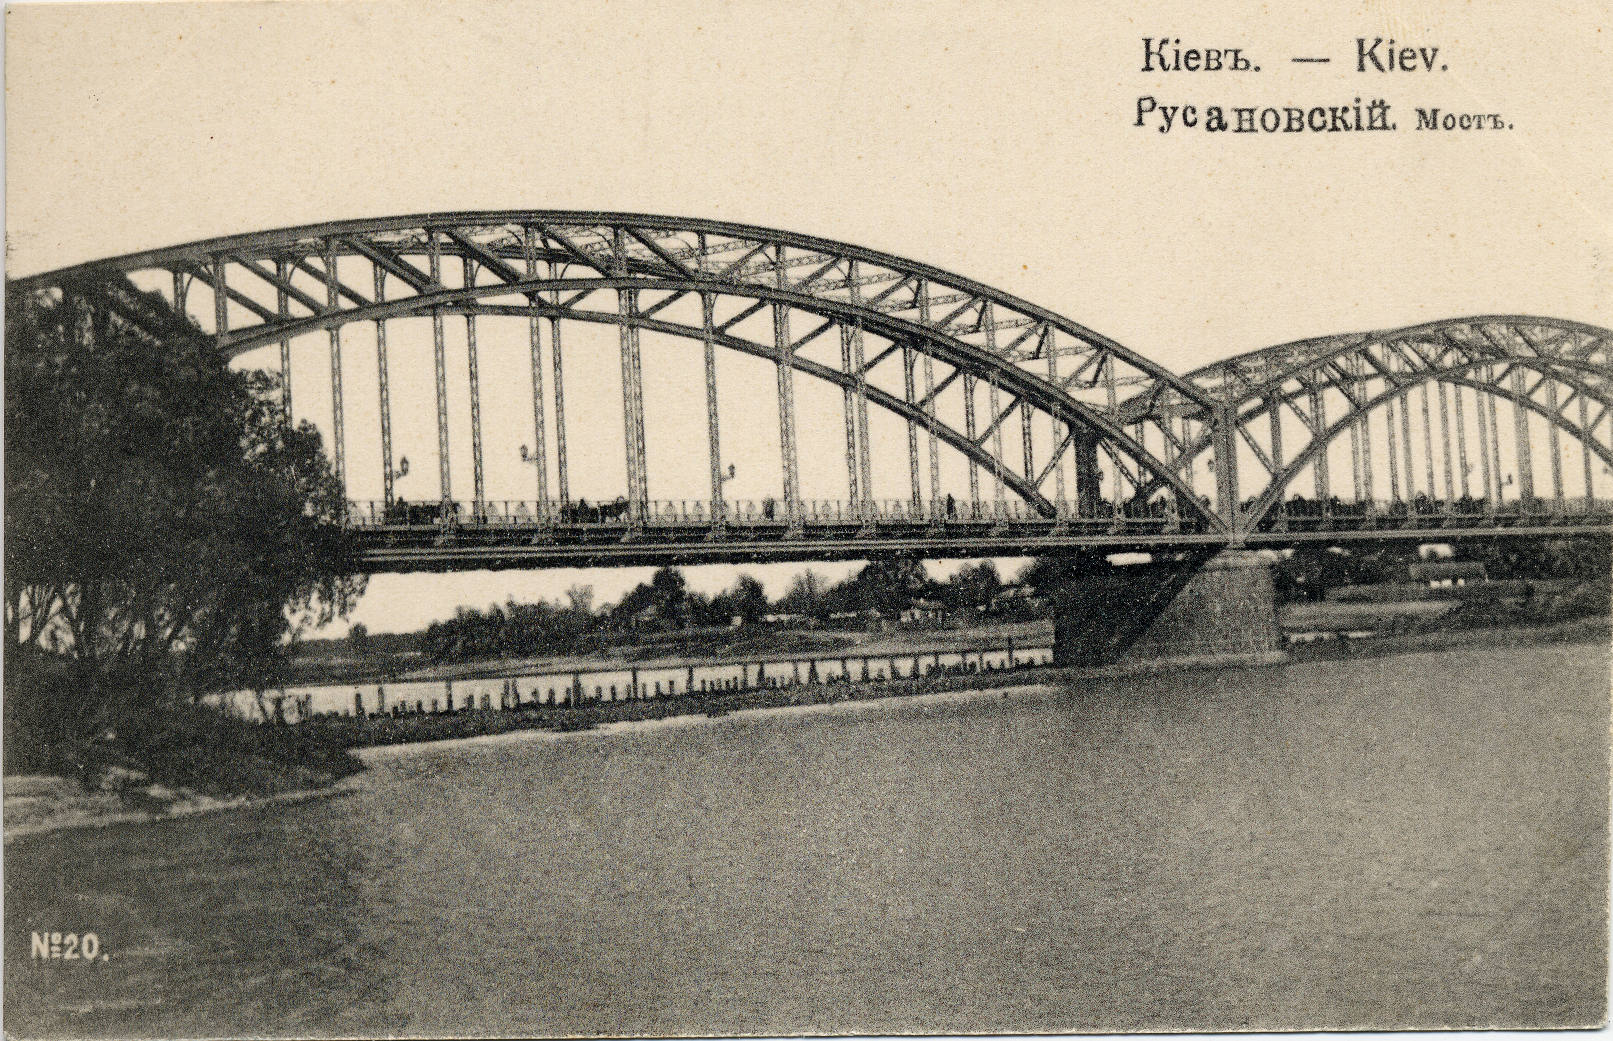
\includegraphics[width=\linewidth]{chast-gorodki/cherto/s_rusmost.jpg}

\textit{Русановский мост. Дореволюционная открытка.}
\end{center}

Депо линии находилось в Никольской слободке. Спустя год открыли вторую линию аж до Броваров\footnote{Эти трамвайные маршруты уже в 1930-х получили номера с 14 по 16, а после Великой Отечественной их не возобновили.}!

Население острова росло. На 1917 год в Предмостной слободке обитало 7200 человек. В северной части поселка были улицы: Днепровская дамба, Баглеевская, Лосенская, Ольгинская, Венецианская, Адамовская, Украинская, Пароходная, Судовая, Мариинская, Тенистая, Монетная. В южной: Русанов вал, Тупая, Южная, Женевская, Успенская, Анненская, Московская, Киевская, Шереметьевская, Трояновская, Струмиловская, Торговая, Николаевская, Днепровская набережная, Заводская, Троицкая, Аскольдовая, Вербиловская, Луговая, Дарницкая, Луговое шоссе, переулки Музен, Кривой, Днепровский. Дома строили на сваях. В половодье жители плавали по улицам в лодках.

Некоторые дворы соседствовали с озерами. Церковь стояла к югу от моста, близко к Днепру – теперь там, у обочины кольца развязки, памятный черного камня крест, заметный из вагона метро, если глядеть в сторону моста Патона. Чуть дальше от берега, вглубь острова, где ныне теннисные корты, шумел базар, а за ним пряталось озерцо. По другую сторону от него, через Броварское шоссе, были пруд, парк с рестораном «Венеция» (он же Петровский, вход от 40 до 50 копеек) и частная дача. Со слободки вело три пути. Западный, на правый берег – через Николаевский мост. Восточный – на Никольскую слободку по Русановскому мосту, через одноименный пролив, естественное продолжение Черторыи. Юго-восточный – по мостику над меньшей протокой Черторыи и дальше в Дарницу.

К концу 19 века Предмостная слободка вновь оказалась на острове, ибо с юго-востока ее отр\'езал от материка Русановский пролив. Он разделялся надвое. Широкий рукав сохранился целиком – ныне он течет вдоль берега Русановской набережной.

А от меньшего рукава, пересекавшего слободку, остались залив в восточной стороне Гидропарка (видно с Русановского моста, за лодочной станцией) и озеро посреди острова. Именно через этот пролив был мостик к дороге в Дарницу, когда большее, второе русло пролива существовало как цепь озер и по суше между ними шла дорога.

Так восстановился уже некогда существовавший отрезок низовий русла Черторыи, да снова образовался остров, омываемый Днепром и Черторыей – будущий Гидропарк. Русановский пролив от моста Метро (левобережного участка) доходит до моста Патона и воды его смешиваются с днепровскими.

В 1877 году цепь озер превратилась в полноценный, большой пролив. Гидрограф Максимович пояснил причину:

\begin{quotation}
Весною 1877 года, при весьма высоком подъеме весенних вод, деревянные мосты в Днепровской дамбе были снесены водою, а в отверстие наибольшего из них, так называемого Русановского, образовалось новое речное русло, по которому направилось речное течение со значительной силой. 
\end{quotation}

\newpage
\vspace*{\fill}
\begin{center}
\includegraphics[width=\linewidth]{chast-gorodki/cherto/\myimgprefix pslob02.jpg}

\textit{Предмостная слободка дореволюционная.}
\end{center}


\begin{center}
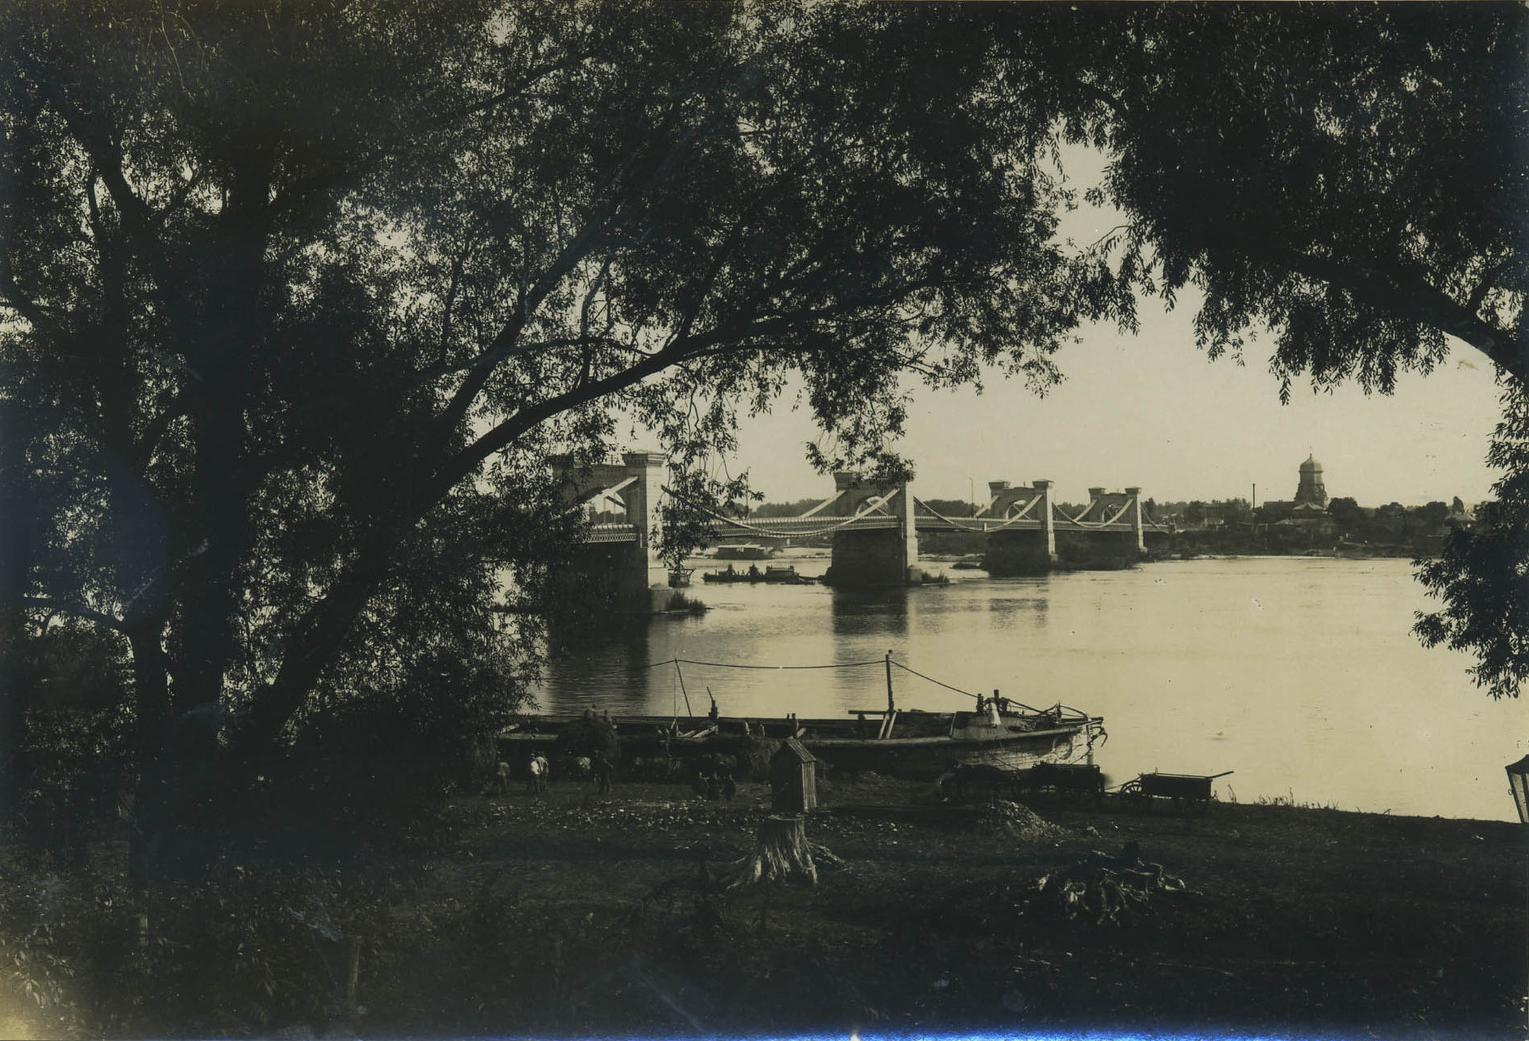
\includegraphics[width=\linewidth]{chast-gorodki/cherto/predm-s-prevber.jpg}
\textit{Вид на слободку с правого берега.}
\end{center}

\vspace*{\fill}
\newpage
\vspace*{\fill}
\begin{center}
\includegraphics[width=\linewidth]{chast-gorodki/cherto/\myimgprefix pslob03.jpg}

\textit{Предмостная слободка дореволюционная.}
\end{center}


\begin{center}
\includegraphics[width=\linewidth]{chast-gorodki/cherto/\myimgprefix 3265.jpg}

\textit{Вид с нее на правый берег.}
\end{center}
\vspace*{\fill}
\newpage
\vspace*{\fill}
\begin{center}
\includegraphics[width=\linewidth]{chast-gorodki/cherto/\myimgprefix 546547567.jpg}

\textit{Вид на нее с правого берега.}
\end{center}

\begin{center}
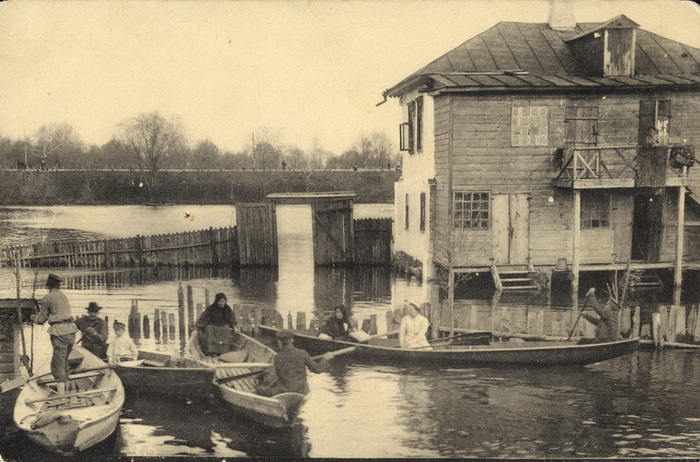
\includegraphics[width=\linewidth]{chast-gorodki/cherto/predmost.jpg}

\textit{Половодье в слободке.}
\end{center}
\vspace*{\fill}
\newpage

На Русановской набережной есть Плавни. Это поросший лозами мыс, где вовсю дымят шашлыками, пьют пиво, громко включают музыку и отчаянно мусорят – словом, весь тот набор почестей, которые способен оказать природе современный киевлянин. Там же дикий пляж, доходящий до бетонного северного берега Русановского канала. 

Я помню Плавни восьмидесятых годов, тихие и чистые, запах ивняка, какие-то старые деревянные лодки в мелких заводях. Весной, местные ходили сюда ломать на продажу «котики», пушистые соцветия вербы.

Плавни лежат напротив места, где Русановский пролив раздваивался. В 1950-х мыс Плавней еще более выдвигался на запад, почти перешейком между материком и островом, прорезанный двумя руслами. И если бы не очередное вмешательство человека, то протоки, при тогдашней системе запруд, снова бы обмелели и Гидропарк превратился в полуостров.

В восьмидесятые, от Русановской набережной на восточный берег южной части Гидропарка ходил катер. Узкий пляж, белый песок, лозы. 

С другой стороны острова, напротив парка Примакова, тоже был пляж, и причал с катером. Тот пляж считался нами, жителями Зверинца, главным. Я тогда не воспринимал его как Гидропарк, хотя так называли весь остров.

Гидропарк для меня был связан с аттракционами, куда мы добирались на метро. Еще не воняло шашлыками, люди мирно гуляли по бетонным плитам дорожек и пили воду из фонтанчиков.

Дорожки приводили нас с мамой к цепным каруселям и качелям-лодочкам. К сталкивающимся, с резиновыми буферами, электрическим машинкам, что сыпали искрами и пахли горелым. К павильону игровых автоматов. Как я любил морской бой! Суешь лицо в пахнущую резиновую маску перископа. Видишь в зеленом свете поле боя, а руки лежат на таком руле с гашеткой. Под большим пальцем кнопка выпуска торпеды. Пууу! И враг повержен.

Больше всего мне нравились американские горки, но катался на них я всего дважды. Страшно! Вышка, с нее два дюжих мужика пускают по деревянному желобу вагонетки. Желоб идет буграми вверх-вниз и потом ныряет в бетонный тоннель, что едва не сносит тебе голову. Я не знал, что в Гидропарке были вещи страшнее.

Незадолго до освобождения Киева советскими войсками, 26 сентября 1943 года немцы стали жечь Предмостную слободку, купно с Никольской и поселком на Трухановом острове. Через обе слободки наши прорывались с боем. 28 сентября в час дня подразделения 56-й гвардейской танковой бригады\footnote{Из состава 3-й танковой армии генерала  Рыбалко.} вошли в Никольскую слободку, но были остановлены тремя противотанковыми рвами и минным полем. Обезвредив 250 мин, подразделения пошли дальше на Предмостную и к пятнадцати часам освободили ее от немцев.

В боях за окрестности Дарницы участвовали также части 163-й и 136-й дивизии 50-го стрелкового корпуса 38-й армии Воронежского фронта\footnote{50-й стрелковый корпус генерала Мартиросяна, 136-я стрелковая дивизия полковника Пузикова, 163-я стрелковая   дивизия полковника Ф. В. Карлова.}. В тот день, выбивая врага из-под Броваров, чтобы подойти к Дарнице, в бою участвовала Мария (Маруся) Лагунова, двадцатидвухлетняя механик-водитель танка Т-34. Родом с Урала\footnote{Родилась в деревня Оконечниково Катайского района, в четыре года осталась без матери, окончила пять классов школы, перебралась к сестре в Свердловск, работала нянькой, в 16 лет устроилась на «Уралобувь» электриком, в свободное время училась водить заводской грузовик.}, доброволец. Фрицы подбили ее танк из пушки. Маруся лишилась обеих ног, однако научилась ходить на протезах без помощи костылей и вернулась в армию\footnote{Долгие годы солдаты танковой части, где служила Лагунова, считали, что она умерла под Броварами, ибо командованию доложили, будто Маруся скончалась от ран по пути в госпиталь. Уже после войны однополчане узнали из прессы, что Лагунова жива, и связались с ней.}. Демобилизовалась уже после войны.

Прожила достойную жизнь, умерла в 1995-м, в Броварах. В былое время там каждый знал, где живет Лагунова – на улице Энгельса. Ныне память хранит музей школы №41, да улица, названная в честь Маруси. 
\vspace*{\fill}
\begin{center}
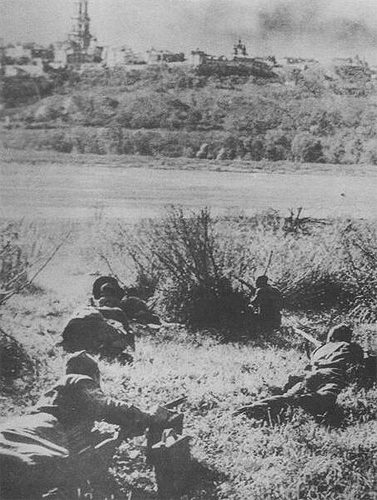
\includegraphics[width=\linewidth]{chast-gorodki/cherto/predmost-j.jpg}

\textit{Наши залегли в Предмостной слободке, напротив Лавры.}
\end{center}
\vspace*{\fill}
\newpage
\vspace*{\fill}
\begin{center}
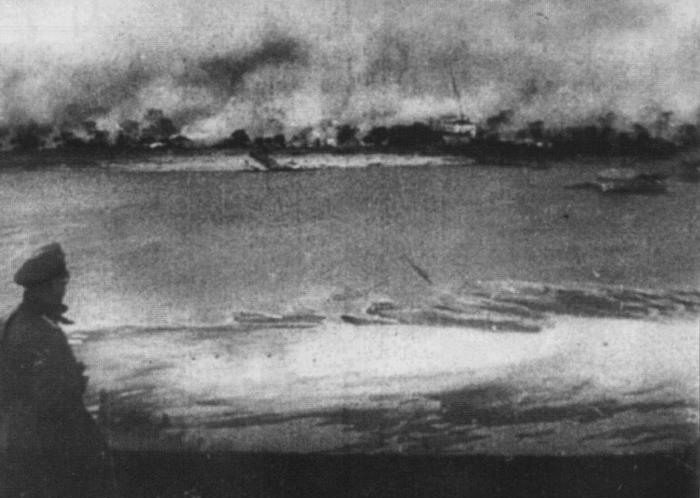
\includegraphics[width=\linewidth]{chast-gorodki/cherto/predmpojar-j.jpg}

\textit{Гитлеровец наблюдает за гибелью Предмостной слободки.}
\end{center}
\vspace*{\fill}
На восток от Предмостной, через Русановский мост над Черторыей (или, если угодно, начало Русановского пролива), лежала Никольская слободка («дальняя Никольская слободка», основная), теперь это окрестности станции метро «Левобережная». Обе слободки в быту часто совмещались, назывались просто Слободкой, или же именование Никольской распространялось и на Предмостную. Никольская «континентальная» прожила долгую жизнь, постепенно застраиваясь новыми зданиями. Еще в 2005 году на месте нынешнего супермаркета «Новус», почти против станции метро были остатки частного сектора. На видео это можно посмотреть в самом конце \href{http://www.archive.org/download/Kaleidoscope/kld_mpeg4.avi}{фильма «Калейдоскоп»}, снятого любительской студией «Дрымба». За строительным забором, во фруктовом саду запорошило снегом хату с проломленными стенами из дранки, деревянный сарай, будку туалета. И сад тот вырубили.

\newpage
\vspace*{\fill}
\begin{center}
\includegraphics[width=\linewidth]{chast-gorodki/cherto/\myimgprefix nslob.jpg}

\textit{Никольская слободка на дореволюционной открытке.}
\end{center}

\begin{center}
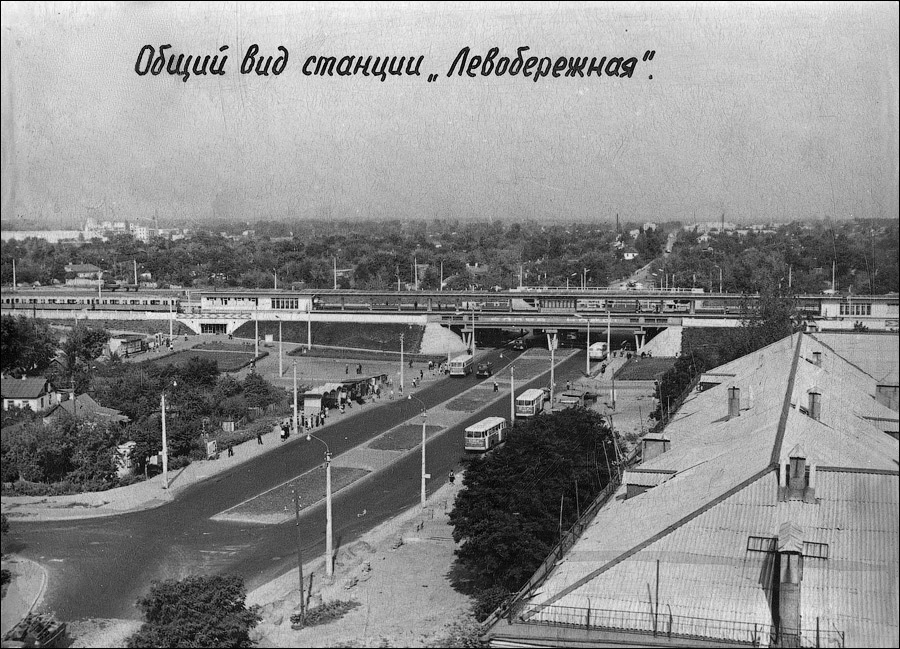
\includegraphics[width=\linewidth]{chast-gorodki/cherto/8865d6c145cea5226cd9f1a60f599465.jpg}

\textit{1960-е, вид на метро с юга.}
\end{center}
\vspace*{\fill}
\newpage
\vspace*{\fill}
\begin{center}
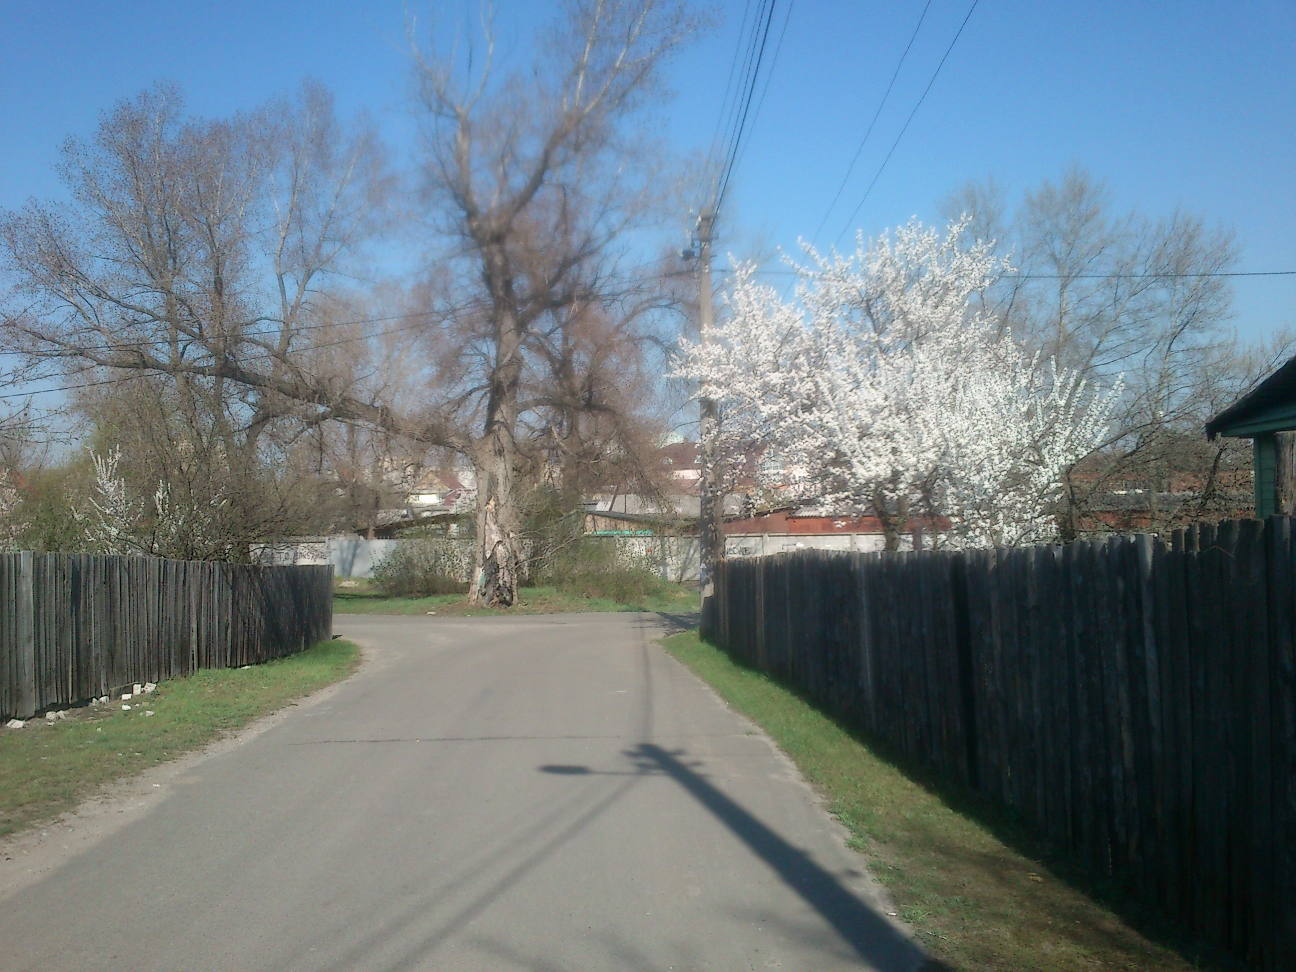
\includegraphics[width=\linewidth]{chast-gorodki/cherto/s_niksl_DSC_0044.JPG}
\end{center}

\begin{center}
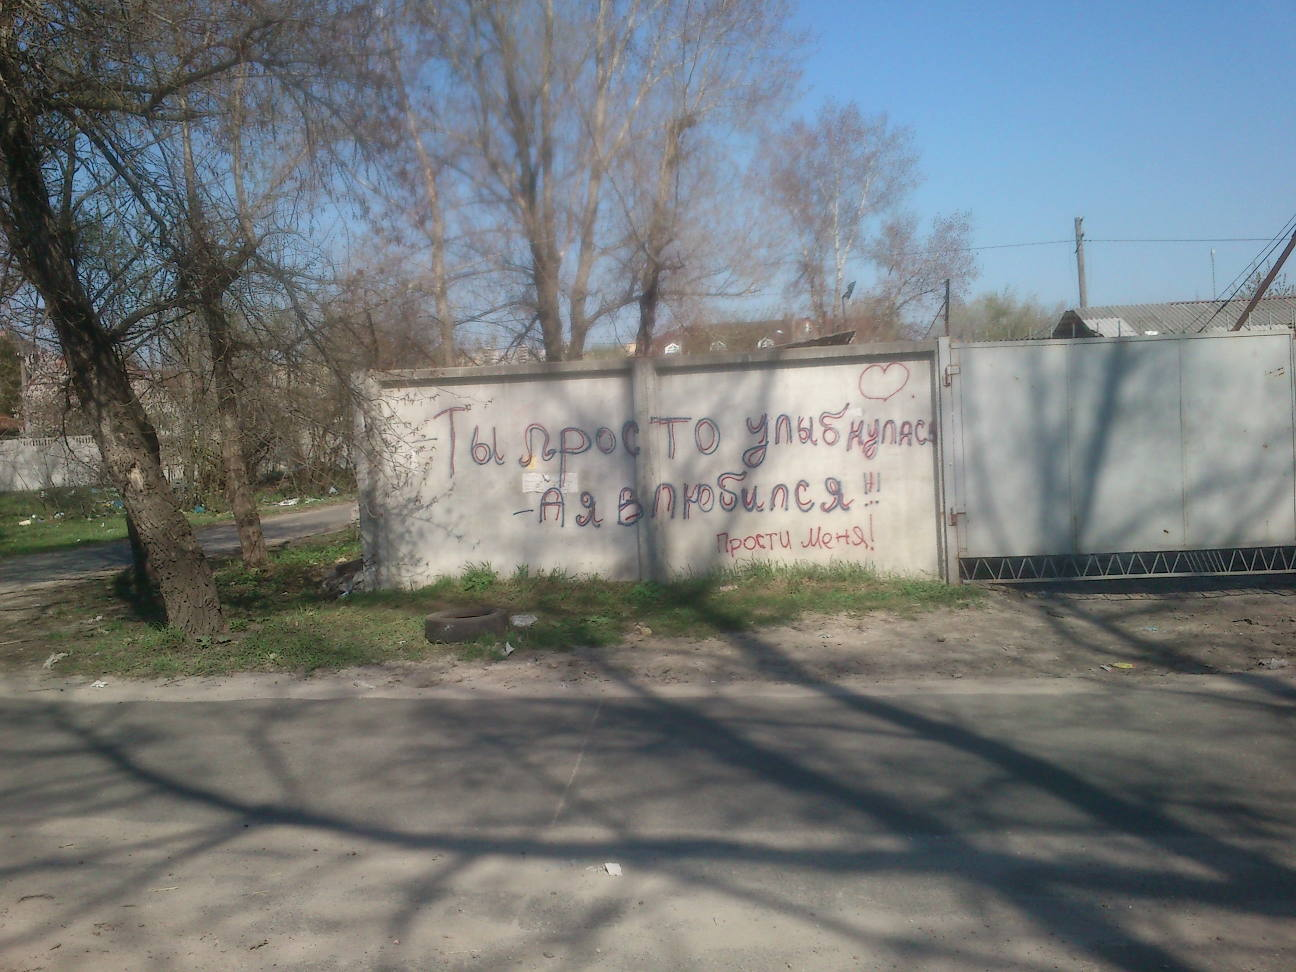
\includegraphics[width=\linewidth]{chast-gorodki/cherto/s_niksl_DSC_0048.JPG}
\end{center}

\textit{На снимках 2013 года – северная часть слободки.}
\vspace*{\fill}
\newpage

К Никольской слободке, северной ее части, относится и частный сектор, примыкающий с юга к Русановским садам, там где улицы Сагайдака, Чаадаева, Силикатная, Комбинатная (от Дарницкого комбината строительных материалов и конструкций, к нему подходила Комбинатная и ветка железной дороги). На 2016 году большая часть территории завода застраивается жильем.

В восточной части слободки, точно перед нынешней больницей №2 на основной районной улице – Луначарского, было слободское кладбище. Теперь там сквер.

Еще одна потеря слободки – озеро Свят\'ище, Святищево или Свят\'ыще, занимавшее место юго-восточной части Русановского канала от моста возле улицы Раисы Окипной и до моста около улицы Ованеса Туманяна. Иначе говоря, часть канала на отрезке вдоль улицы Флоренции раньше был озером. Впервые я встретил его на моем любимом плане Даниила де Боскета 1750 года:

\begin{center}
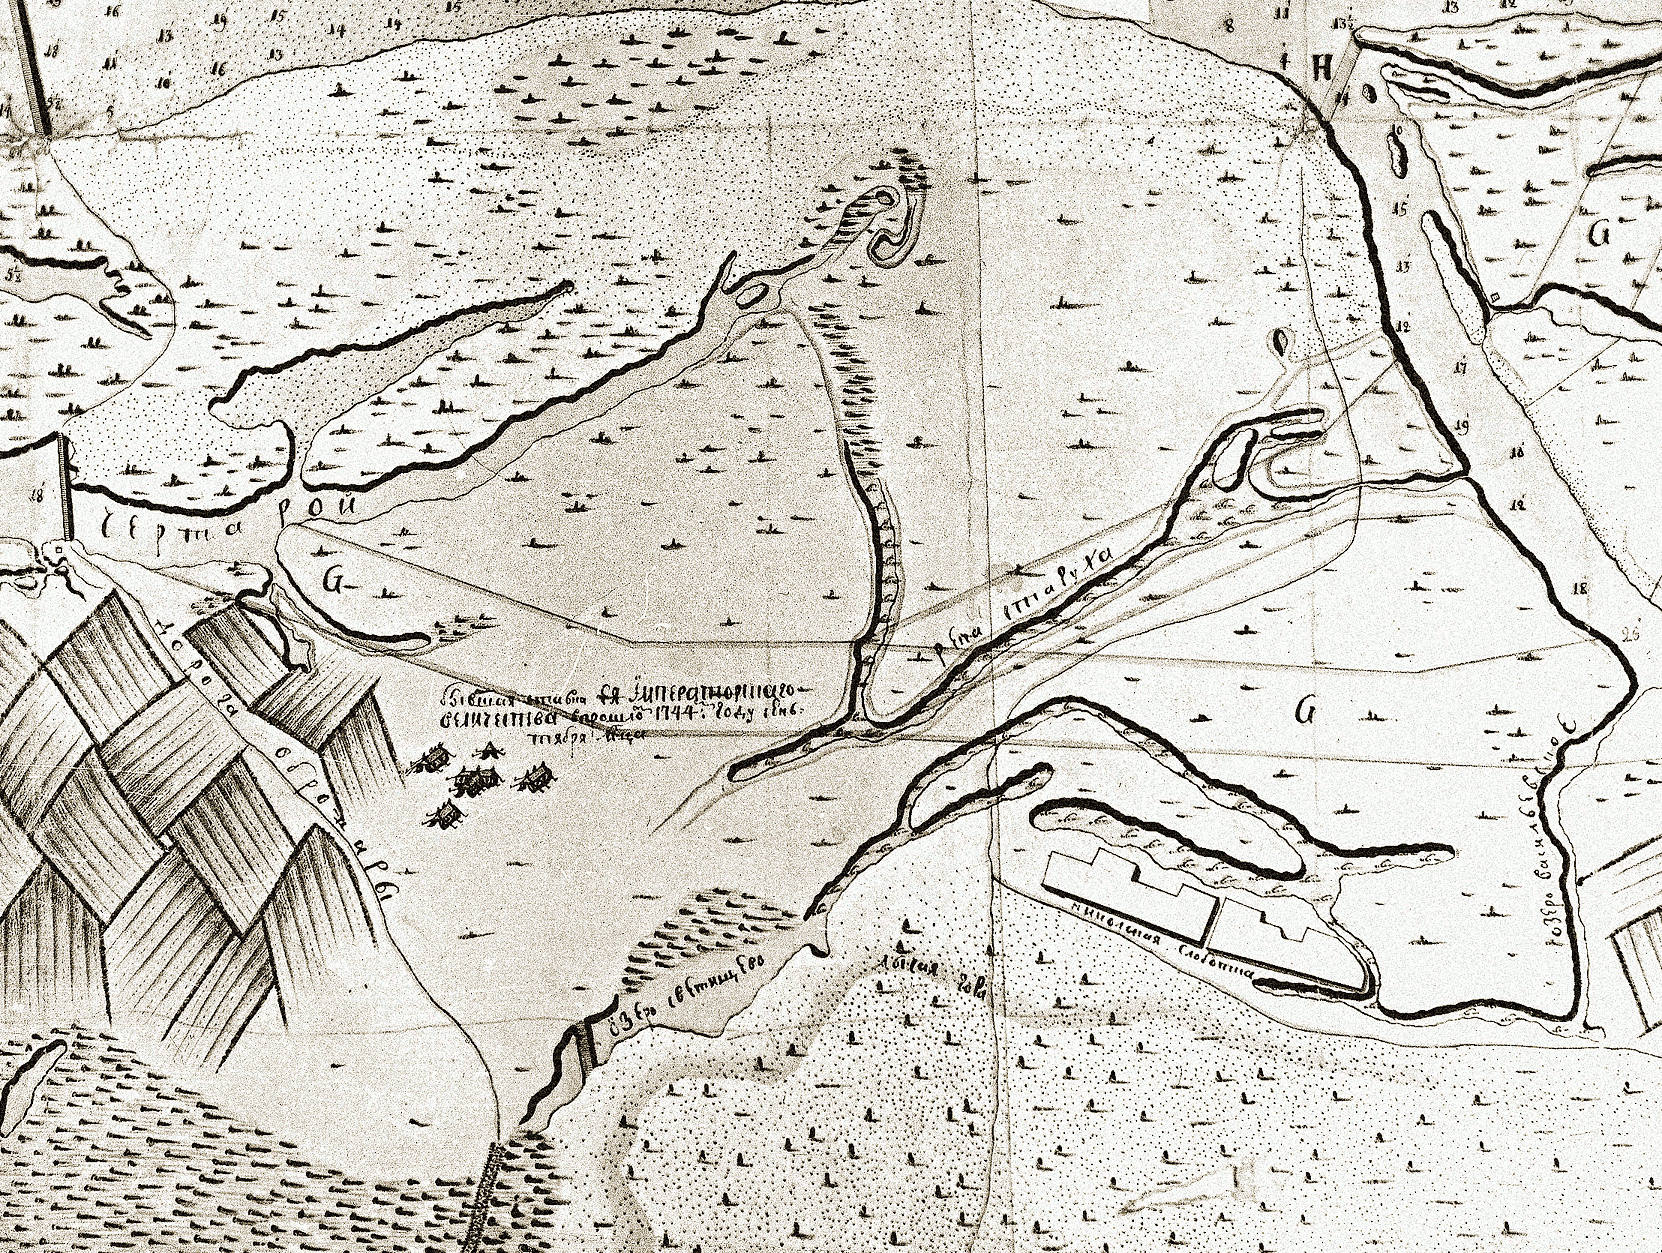
\includegraphics[width=\linewidth]{chast-gorodki/cherto/s_svyat-1750.jpg}
\end{center}

Здесь видно – к югу (слева) от Никольской слободки, но севернее «дороги в Бровары» – Лысую гору и озеро «Светищево» с мостом через оное. 

Лысую гору мы обсудим позже. Сейчас про озеро. Некоторые краеведы полагают, что оно сгинуло еще в начале 20 века, однако на аэрофотоснимке 1943 года длинное Святище – вот оно, живо-здорово, в середине картинки:

\begin{center}
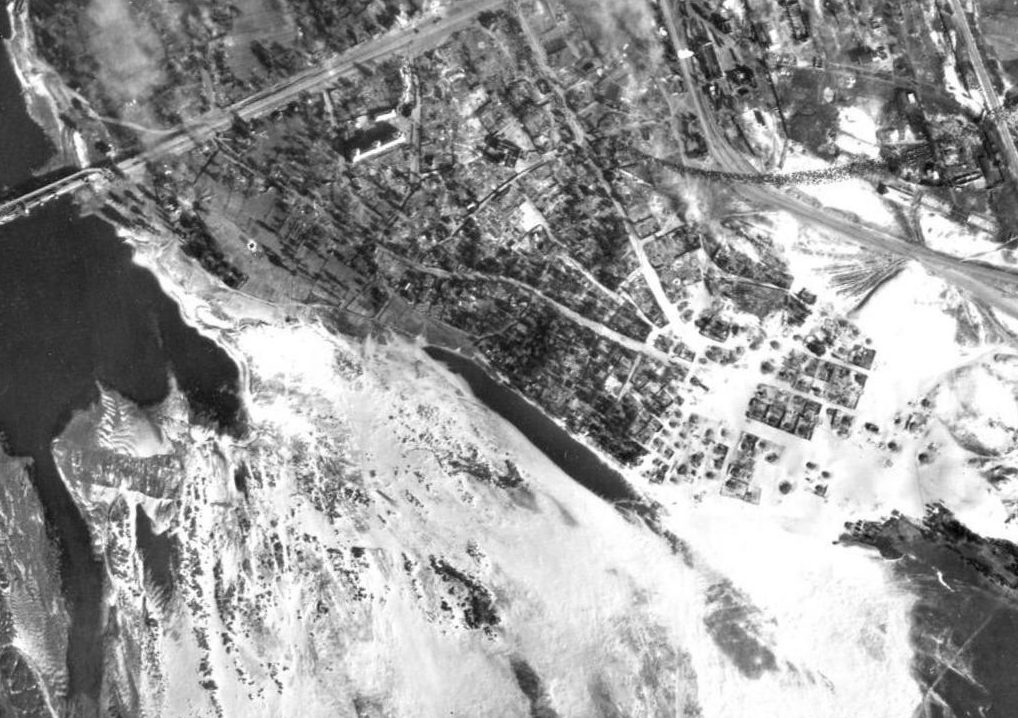
\includegraphics[width=\linewidth]{chast-gorodki/cherto/svyat-1943.jpg}
\end{center}

В то время параллельно северному берегу озера проходила улица Лозовая, да к самому озеру шли два проулочка.

Именно на берегу бывшего Святища, в конце улицы Туманяна стоит высотный дом номер 8, последний адрес актера и режиссера Леонида Быкова. Вообще Русановский канал почти точно вписался в изогнутую цепь тамошних водоемов, сохранившихся на 20 век – Святище, болото, Тельбин.

Сейчас на картах именем «Святище» обозначено другое озеро, на Осокорках.

А как долго я весной 2013 года искал настоящее Святище, не зная тогда об аэрофотоснимке! В первый день поиска я бродил между станцией метро «Левобережной» и Русановским каналом, одетый по случаю отцовского дня рождения в солидный пиджак. Много лет, после детства, я не носил пиджаки, а этот подкупил меня обилием карманов и подкладкой, не вызывавшей судорог души. Я вглядывался в каждую низину между домами. Потом поехал туда же на велике, и во глубине дворов нашел большую ложбину, с детской и баскетбольной площадками. Где и заподозрил Святище, пока не понял по аэрофотоснимку и новым для меня картам, что озеро поглощено каналом.

\begin{center}
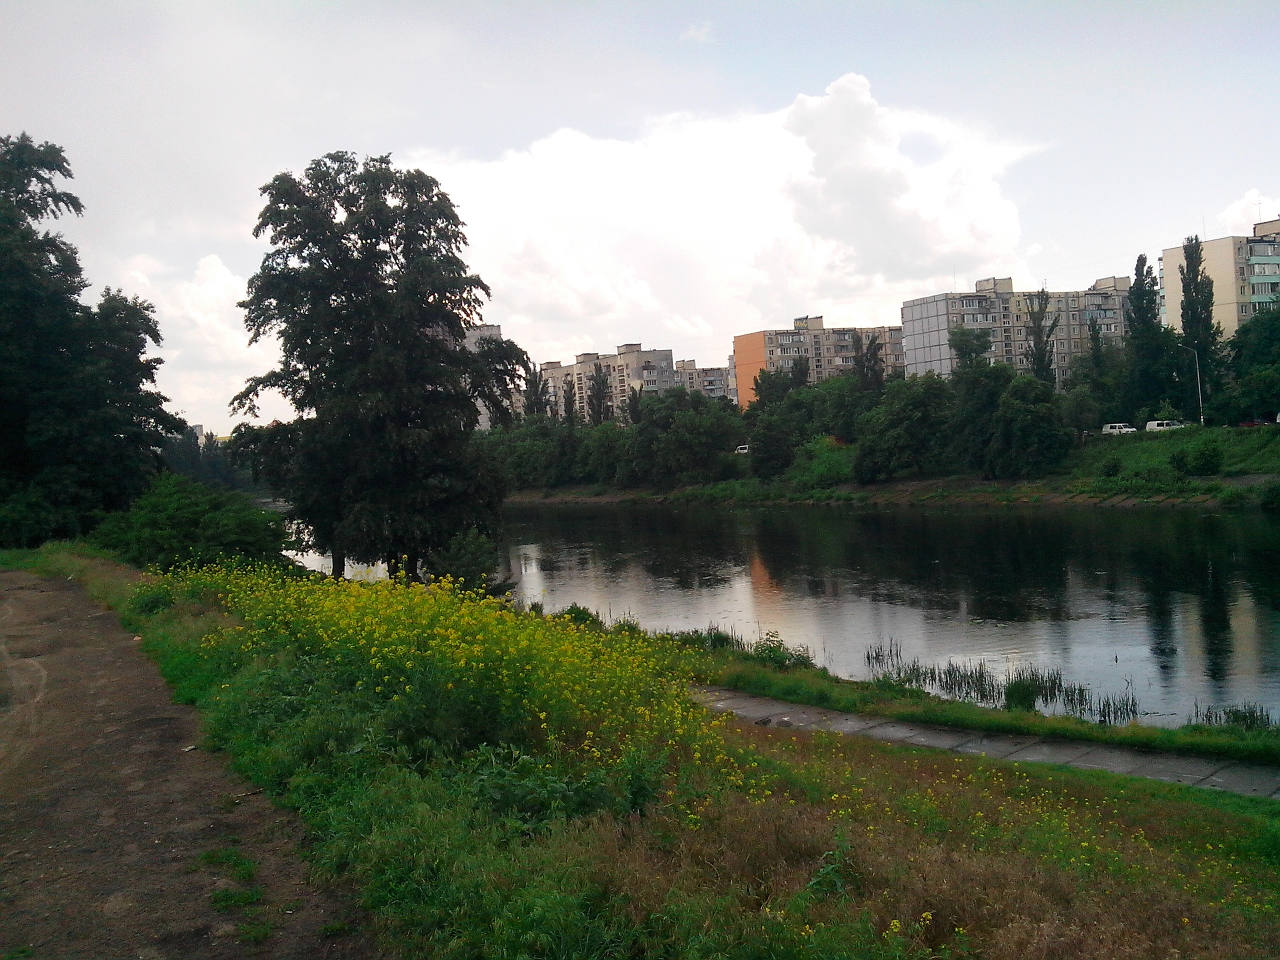
\includegraphics[width=\linewidth]{chast-gorodki/cherto/s_svyat-IMG_20140527_134118.jpg}
\textit{Тут было озеро Святище. Май 2014 года.}
\end{center}

В XXIX томе журнала «Киевская старина», за 1890 год, помещена статья археолога Николая Беляшевского\footnote{Любопытно, что Беляшевский вел раскопки и близ другой Лысой горы, на Кирилловских высотах, где исследовал знаменитый Курган-могикан.} «Первобытный человек на берегах р. Днепра», где он рассказывает о находках возле Святища. Ценность этого сообщения еще и в описании места, каким оно было в конце 19 века:

\begin{quotation}
Бугры у с. Никольской Слободки. С. Никольская Слободка находится в том месте, где кончаются сооружения Цепного моста и начинается Черниговское\footnote{Ныне Броварское.} шоссе. 

К югу от села, сейчас же за ним, лежит небольшое озеро Свят\'ыще. Песчаные открытые бугры составляют северо-восточный берег этого озера, они простираются затем с одной стороны к лесу, с другой же подходят к постройкам идущим в этом месте по обеим сторонам шоссе.

По другую сторону шоссе пески также обнаруживаются и заканчиваются большим бугром в северном конце села у сельского кладбища. Ближе к лесу бугры покрыты тонким слоем дерна и отчасти окрайной леса.

Обнажения культурного слоя заметны главным образом по берегу озера и на такой высоте, что вода в весенние разливы туда не добирается; в этом можно было убедиться во время сильного разлива весной 1888 г.; местность же между этим берегом озера и противоположным правым берегом Днепра, представляет весной сплошную водную поверхность.

Находки сосредоточивались в двух местах: при начале озера, там, где кончалось село, и даже крайние хаты его уже расположены на обнаженном культурном слое, и затем – почти в конце озера, – здесь культурного слоя почти не было заметно, но зато найдено несколько сосудов.

Случай дал возможность сделать и геологические наблюдения: летом 1889 г. из берега озера брали песок для земляных работ на реке; в образовавшейся выемке было видно, что однородный светло-желтый песок залегает на несколько сажней вглубь.

Внешний вид местность по берегу озера имела следующий: песок окрашен в пепельно-се\-рый цвет, толщина темного слоя различна – иногда достигает 1/4 аршина\footnote{Около 18 сантиметров.} и более, иногда же является как бы тонким налетом. На поверхности разбросаны, а также торчат из песка куски от сосудов с орнаментом и без него, лежат также черепки и кучами, они, по-видимому, принадлежали целым сосудам, распавшимся от действия атмосферы; между черепками много измельченных выветрившихся костей, встречающихся также кучами, и масса осколков кремня и других камней, между ними попадаются и кремневые орудия.

Местами все эти остатки расположены вокруг кострищ, представляющих не особенно большие кучи углей. Это в начале озера. Дальше по берегу культурного слоя не было замечено, но попадались черепки, а при конце озера вблизи кострищь найдены были, как уже сказано, целые сосуды.

[Далее Беляшевский начинает опись находок, привожу ее далее в пересказе.]
\end{quotation}

Целыми нашли немного орудий, большинство же – поломанные. 80 обоюдоострых ножиков из кремня (наибольший из которых был длиной 5,5 см., а шириной 1) отличались, по словам Беляшевского, миниатюрностью, как и все остальные орудия. 7 кремневых острий длиной до 3 сантиметров. Кремневые наконечники стрел около 20 штук, обнаружены почти вместе, там же где осколки кремня. Полсотни овальных кремневых скребков. Про множество поломанных орудий Кибальчич высказал мысль, что их могли разбивать нарочно при погребальном обряде.

Керамические изделия не знали гончарного круга, лепились руками. Беляшевский пишет:

\begin{quotation}
Глина выделывалась различно: встречались (редко) черепки из грубой глины с большою примесью кварца, затем из глины лучшего качества, но все-таки не обладавшей достаточным сцеплением, наконец были из глины хорошо отмученной, неуступающей современной.

Обжиг также различен; это можно видеть на изломе черепков; большей частью обожжена только наружная сторона, получившая от этого красный цвет.

[...]

был также и полный обжиг, прошедший насквозь черепок. Толщина стенок сосудов от 1 1/2 до 1/2 сантиметра.
\end{quotation}

Сосуды были до 20 сантиметров в поперечнике, а высотой до 30 сантиметров. Узоры в виде точек,  прямых линий и зигзагов сделаны по сырой еще глине палочкой, костью, кремнем, веревочкой. Ушек сосуды не имели, вместо этого проделаны дыры ближе к ободу. Среди глиняных предметов Беляшевскому попалось глиняное прясло и обломок другого.

Кроме того археолог нашел там же, в песке, предметы, отнесенные им к более новому времени – бронзовые куски пряжек, перстней, пуговиц, бубенчик, кольцо, трехгранные стрелы. А также железные «стрелы разных форм и ножички».

По уровню гончарного мастерства и отделки кремневых наконечников, Беляшевский отнес культурный слой к концу каменного века и концу его неолитического периода. Ученый полагал, что отыскал здесь стоянку первобытного человека.

И далее в статье дается замечательное, современное ей описание смежной местности, которое нам пригодится, чтобы знать, как выглядел тогда Левый берег:

\begin{quotation}
К северу от Никольской Слободки, на протяжении почти 5-ти верст вплоть до с. Воскресенского, тянется под лесом ряд бугров различной величины и формы\footnote{Речь идет о длинной возвышенности, слывущей Лысой горой – однако не к югу как отмечено на карте 1750 года, а по другую сторону от Никольской слободки, на север.}, покрытых тонким слоем дерна. В некоторых местах дерн разрушился, песок обнажился и, вследствие действия ветра, образовались небольшие котловины; в них попадаются хотя и в незначительном количестве аналогичные с найденными у Никольской Слободки черепки и кремни, так что бугры эти являются продолжением стоянки Никольской слободки.

У села Воскресенского бугры принимают более правильную куполообразную форму и совсем обнажены; находки и здесь были самые незначительные.

Рядом с селом Воскресенским идет ровная песчаная плоскость, не давшая никаких находок; только в конце, где опять начались бугры, найдено несколько отбивных кремней и большая, хорошо подправленная стрела. 

Эти же бугры тянутся далее вокруг болота, отделяющего село Воскресенское от лежащего выше села Вигуровщины. Там, где болото более всего вдается в берег, обнаружено небольшое место, сплошь покрытое осколками кремня, кусками ножиков\footnote{Почему-то всюду не ножи, а ножики – маленькие.}, целыми ножиками и скребками, тут же [...] лежали осколки розоватого песчаника, из которого хотели приготовить орудия.

Между черепками по орнаменту были одинаковые с найденными у Никольской слободки, но нашлось также и несколько особенных, как например орнамент елкой.

Целых сосудов у села Вигуровщины не было найдено, но нам передавали местные пастухи, что весной они часто находили в песке «якись мыски». Встречались в кучах черепки от распавшихся сосудов.

[...]

Далее села Вигуровщины мы не простирали наших изысканий, но в этом месте бугры, продолжаясь немного выше по направлению к селу Троещине, прекращаются и опять обнаруживаются, насколько мы знаем, уже спустя большое пространство\footnote{Подобная цепь песчаных холмов, более короткая – урочище Сухие горы – идет по Быковнянскому лесу параллельно улице Жукова.}.
\end{quotation}

На Никольской слободке, к западу от школы 125 (Плеханова, 2), там где сейчас стадион и пустыри, в 19 веке было иудейское кладбище.

Название «Никольская слободка» осталось в ходу среди местных, остальные больше используют «Левобережка», «Левобережная» – по станции метро, в лучшем случае Никольской слободкой величают квартал между железной дорогой и улицей Никольско-Слободской. По адресу Челябинская, 13 – эдакий последний из могикан, двухэтажный дом, однако насколько он стар я не знаю. Прежде в нем размещались прачечная и фотоателье.

Еще немного о былом административном делении. До революции, Никольская слободка относилась к Остёрскому уезду Черниговской губернии. Когда человек с правого берега достигал по Николаевскому цепному мосту берега левого, Предмостной слободки, то сразу оказывался на окраине Остёрского уезда. Граница шла по линии западного берега Гидропарка.

А Труханов остров относился к Киеву, граница Остёрского уезда проходила по восточному берегу Труханова острова. На Трухановом и Муромце, кроме прочего, располагались городские сенокосы – запасы лошадиного топлива!

В 19 веке, в южной трети нынешнего Гидропарка, был трактир Резанова (Рязанова). Любопытно, что озеро Святищево, известное так допустим в 1750 году, на карте 1799 года подписано как Русаново, а позже мы видим на картах снова Святище. Возможно предки Резанова, коему принадлежал трактир, прежде звались Русановыми и владели землей с тем озером? Впрочем, допустим, на карте 1842 года Русановым озером названо то, что ранее именовалось Васильевским, и на той же карте есть привычное Святище.

Писатель Николай Лесков, живший в Киеве в 1850-х, писал о «грандиозных кутежах в этом трактире Рязанова на Трухановом острове». На плане Шуберта 1863 года издания, трактир стоит, однако, на левом берегу, напротив Лавры, у дороги, что вела с Кухмистерского села\footnote{Прежде это была Кухмистерская слободка.} (там теперь район на запад от Тельбина, между улицами Шумского, Березняковской, Тычины) что лежала около широты Дарницкого моста.

Тарас Шевченко в «Прогулке с удовольствием и не без морали» (1855-1858) упоминает сей трактир:

\begin{quotation}
Перед лицом мартовского солнца сконфузился и почернел белый снег. Ручьи весело зашевелились в горах и побежали к своему пращуру, Днепру-Бело\-груду сказать о приближении праздника богини Яры. С любовию принял лепечущих крошек старый Белогруд и распахнул свою синеполую ризу чуть-чуть не по самые Бровары. Рязанова трактир, как голова утопленника, показывается из воды. А гигант-мост, как морское чудовище, растянулся поперек Днепра и показывает изумленному человеку свой темный хребет из блестящей пучины. Прекрасная, величественная картина!
\end{quotation}

Позже когда Резанов переделал трактир в ресторан с купальнями, лодочной станцией и столиками на воздухе, он стал местом молодежных тусовок. Здесь, далеко от глаз полиции, между студентами и юнкерами нередко случались побоища. Около заведения Резанова собирались для начала конных прогулок к паромной переправе на Десне.

В советское время, до превращения Русановки в остров, там был рыболовецкий хутор – между современными улицей Энтузиастов, Шамо, набережной и Русановским бульваром. Режиссер Довженко сидел на заливном лугу неподалеку, любовался видом и мечтал купить тут хату.

Мечты часто не сходятся с делом – так и я желал в этой главе последовательно двигаться с севера на юг в описании островов, а сразу прыгнул от устья Десны к Гидропарку. Усилием воли возвращаю себя в начало. Если не касаться двойственной природы Гидропарка, что волей обстоятельств превращался из полуострова в часть материка и наоборот, да не считать изменчивого Долобецкого, раньше между Днепром и Черторыей было только два огромных острова. Северный – Муромец, и южный – Труханов. Да и то, земли Муромца, насколько я понимаю, стали островом только в 17 веке.

На современных картах Муромец ошибочно показан в урезанном виде. Истинный Муромец – это от устья Десны и до Московского моста. Оттуда к Петровскому железнодорожному, что переброшен с Рыбальского острова к дачным участкам Русановских садов, сейчас лежит суша с дорогой, а раньше, еще в 19 веке, там был Пробитец – пролив из Днепр в Черторыю.

Парк Дружбы Народов – это тоже Муромец. Муромец – напротив Оболони, а Труханов – напротив Подола и набережной в направлении  мостов Пешеходного и Метро.

\begin{center}
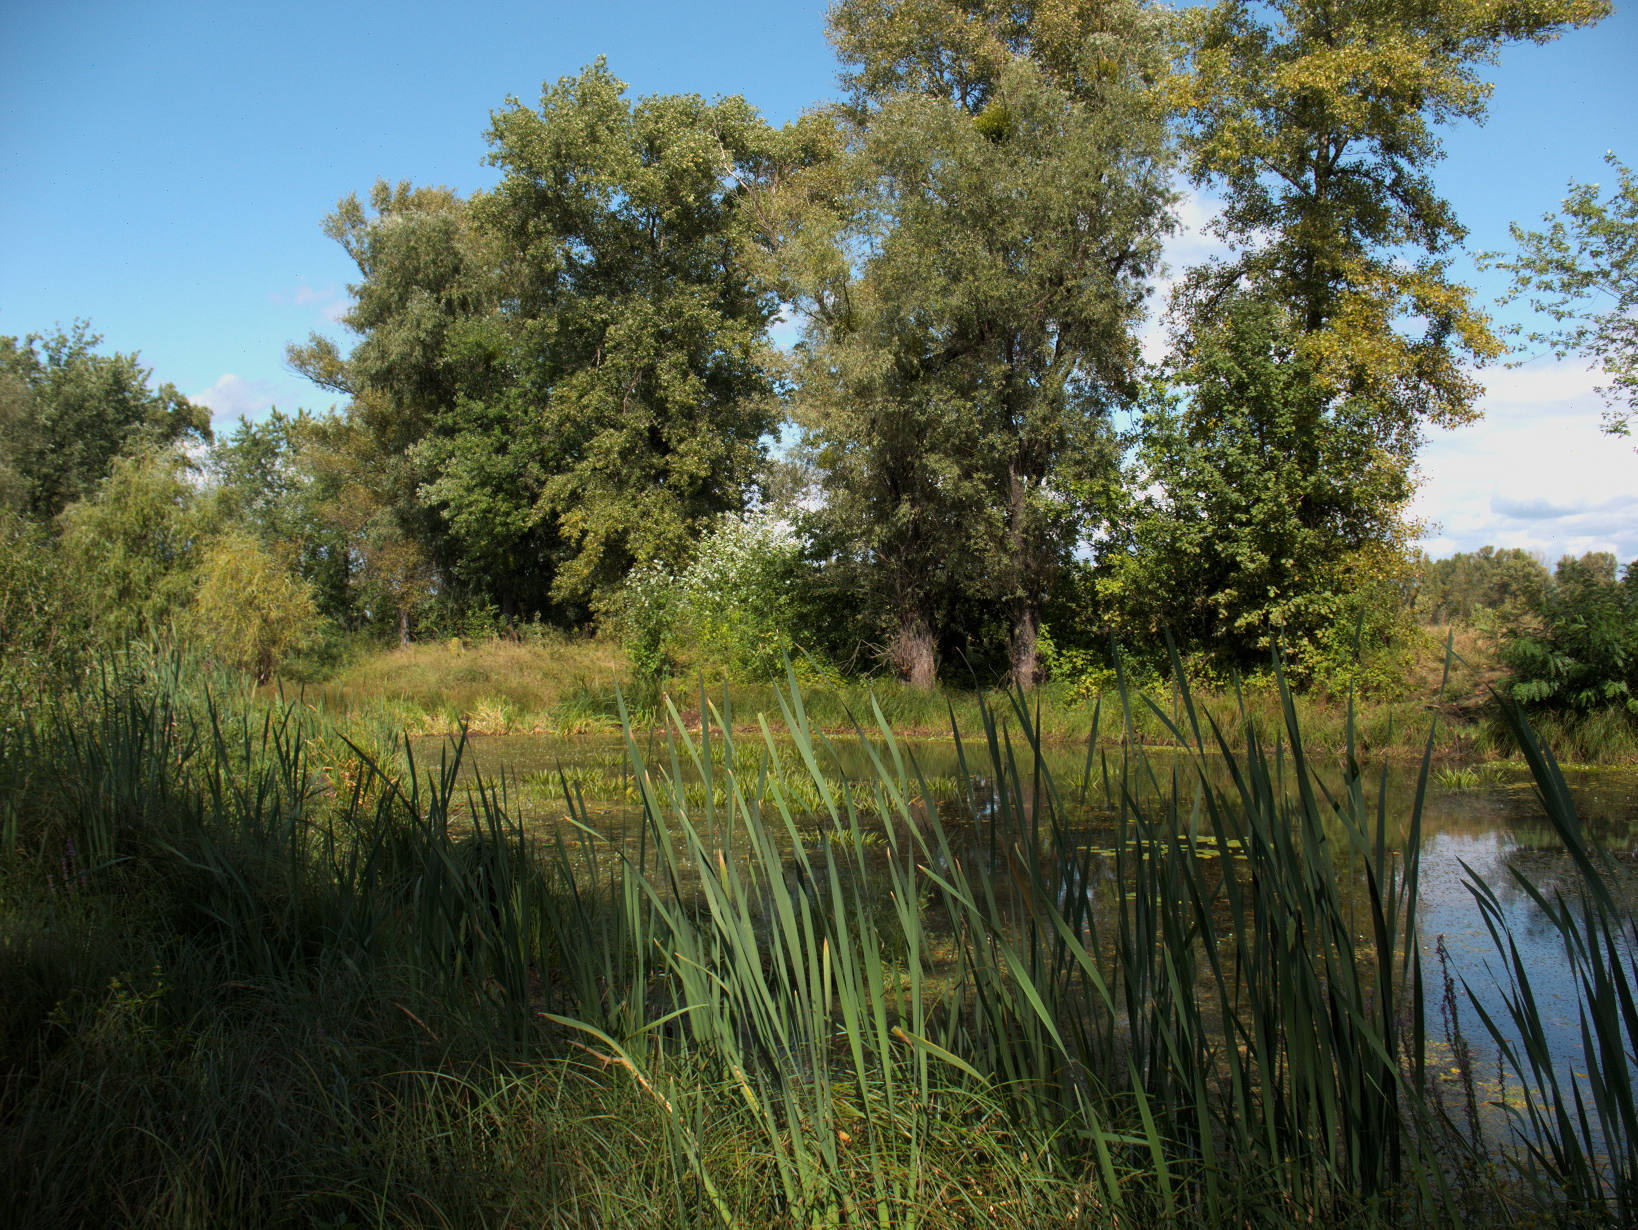
\includegraphics[width=\linewidth]{chast-gorodki/cherto/s_CRW_3908.jpg}

\textit{Одно из луговых озер на Муромце.}
\end{center}

Раньше Муромец назывался Муравец, и на нем был одноименный хутор. А может Муравец – искаженное Муромец, не знаю. Сейчас на острове расположен предваряемый генделыками парк Дружбы народов, северной частью раскинувшийся в просторы с грунтовыми дорогами, где любят кататься велосипедисты. Одно из красивейших мест в Киеве. Раньше так выглядела Оболонь – широкое поле с луговыми озерами, зелеными дубравами, рощами под чистым небом.

Восточным берегом Муромец выходит к Черторые, северным – к Десне и ее устью, с запада омывается Днепром. На современных картах острова много чего напутано, и я разложу сейчас всё по полочкам.

Парк Дружбы Народов, наискось от Десенки к Днепру, пересекается проливом, который лоции стыка 20 и 21 веков обозначают «заливом Бобровней». Но это Небышевка, а не Бобровня. Урочище Бобровня выше, в северной части острова.

На берегу Днепра лежал хутор Небышевка, по нему и окрестным землям так именовался и сей пролив, а скорее – канал. Владел хутором генерал-майор и гвардии майор Василий Васильевич Нейбуш, обер-комендант Киево-Печерской крепости с 1730 по 1737 год, исполнял также обязанности губернатора Киевской губернии.

\begin{center}
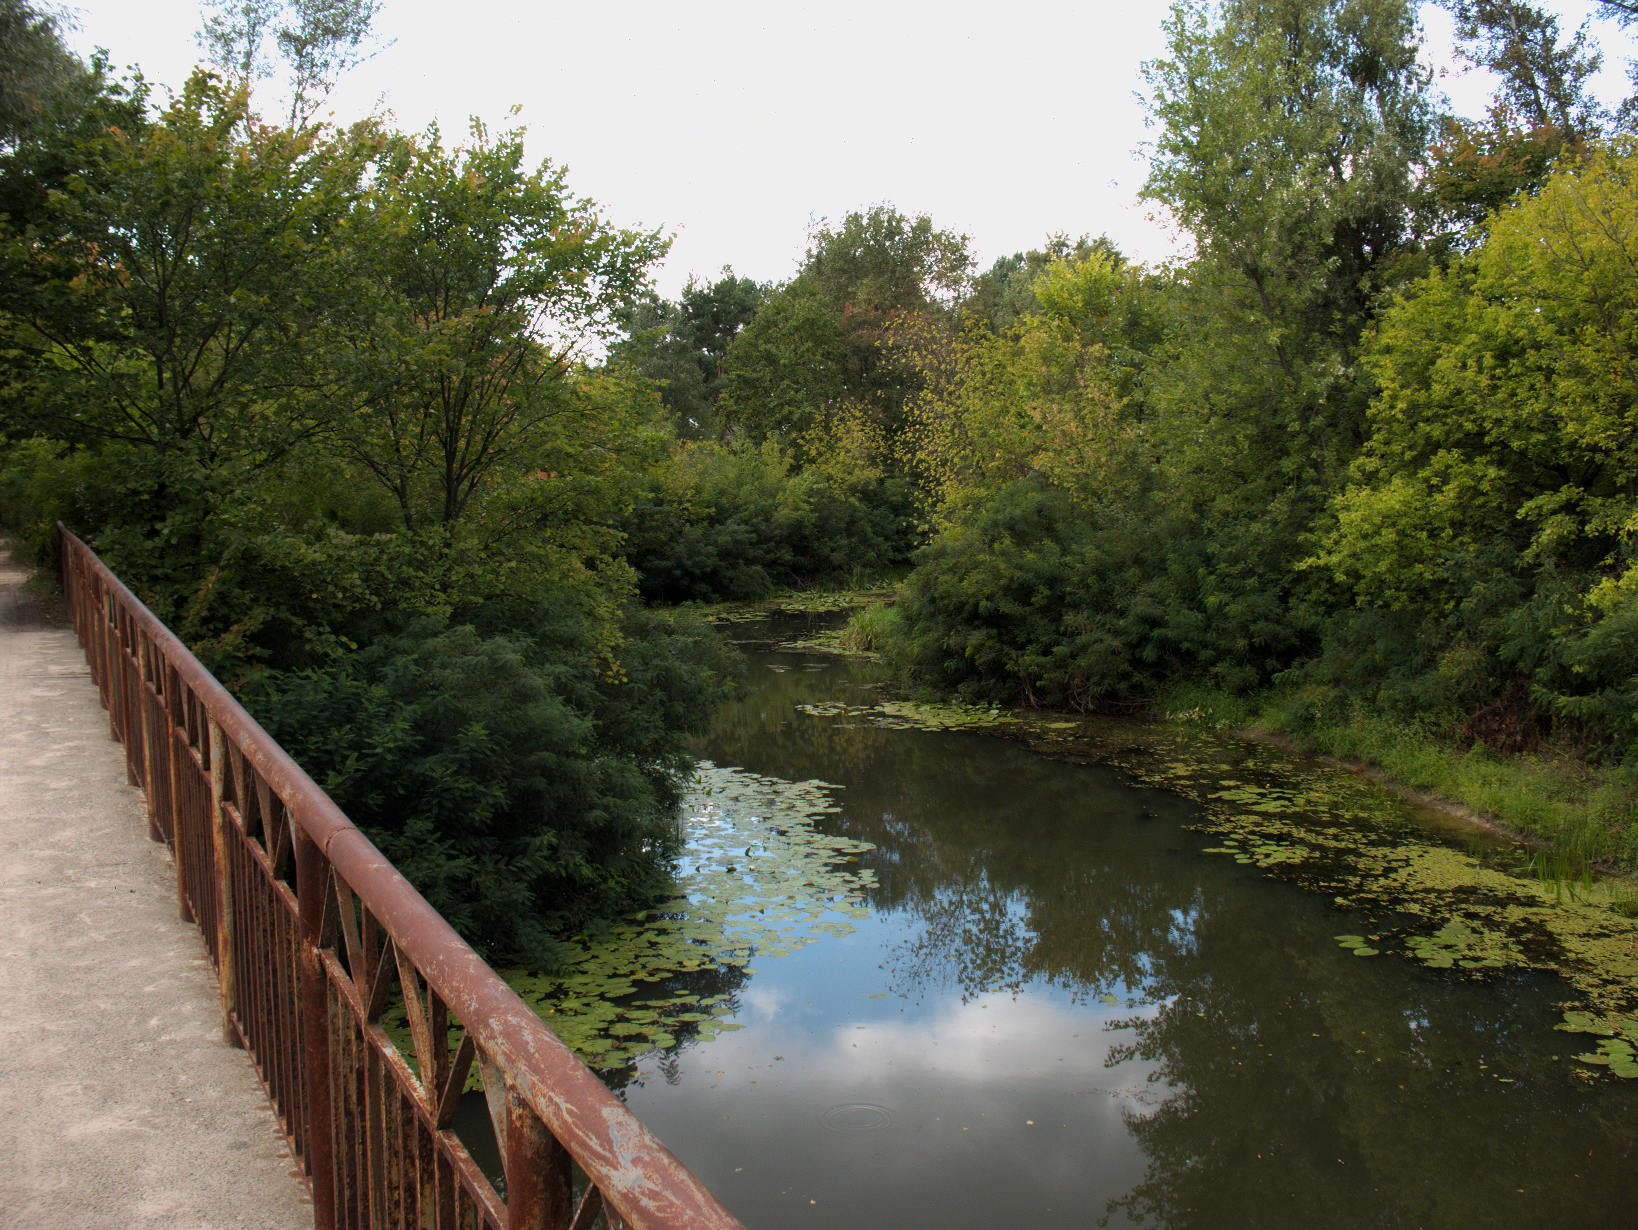
\includegraphics[width=0.80\linewidth]{chast-gorodki/cherto/s_mur_CRW_3939.jpg}

\textit{Современный пролив Небышевка. 2014 год.}
\end{center}

С начала 20 века русло Небышевки сохраняет очертания, включая отклонение на восток у северного конца, у бывшей Небышевской запруды – кажется, боковой канал хотели провести дальше до Черторыи.

Исток Небышевки на западном берегу Муромца начинается примерно по широте Собачьего Гирла на противоположном берегу Днепра. Он завален камнями, через них просачивается ручей с днепровской водой. По камням перебираются на другой берег Небышевки. А ее устье выходит в Черторыю, и там пролив легко перейти вброд. Через Небышевку перекинуто несколько мостов, соединенных с грунтовками. Частые здесь велосипедисты переезжают южным мостиком на другую часть острова, катаются по тамошним просторам, и через северный мостик возвращаются. Или наоборот.%\footnote{Словом «Муромец» щеголяют немногие велосипедисты, местность в-основном слывет у них как «ПДН» – парк Дружбы Народов. Ездят среди лугов, к устью Десны.}.

Вода в проливе течет между довольно высокими берегами и возникает мысль, что канал этот – рукотворный, прорытый, дабы не плыть вокруг острова. Почти на всем протяжении Небышевка спрятана за кустами и деревьями. Вот я написал «вода течет», а на деле я не знаю подробностей о течении. Спокойная гладь с пятнами кувшинок, камышом и ряской, откуда моргают глазами жабы. Но легко представить, что прежде это был удобный водный путь. Да и сейчас, если бы не водная растительность, по нему свободно поплывут лодки. 

И вот Небышевку на всех современных картах, включая лоции\footnote{Удивительно, что на лоциях остался параллельный заливу «перекат Небышевский». Перекатом называют отмель поперек реки, в месте быстрого течения, с глубоким дном по обе стороны мели.} переименовали в Боловню или Бобровню! Но Бобровня – совсем другое. Бобровня, или Бровня\footnote{По Далю: «веретья, боровой кряж, гребень, с хорошим лесом».} – известное по документам с 17 века озеро. На карте Шуберта оно обозначено на широте чуть ниже тогдашнего положения села Троещины, с 1877 года сместившейся прочь от берега на восток. На карте лоций 1914 года остается «урочище Бобровня», ниже озера Малое Кинище, на широте современной улицы Марины Цветаевой. Ныне просто Кинище подписывают Кильнищем, а Малое Кинище – болотом Подковой.

А на плане Сноевского у берегов «речки Бобровни» обозначено городище. Взяв в руки современную карту, где Бобровней подписан другой водоем, Небышевка, вы будете полагать, что городище находится там, а не в окрестностях современного Кинища! Кстати, на плане Сноевского вообще не отражено озеро Кинище, но в том месте протекает «Бобровня».

\begin{center}
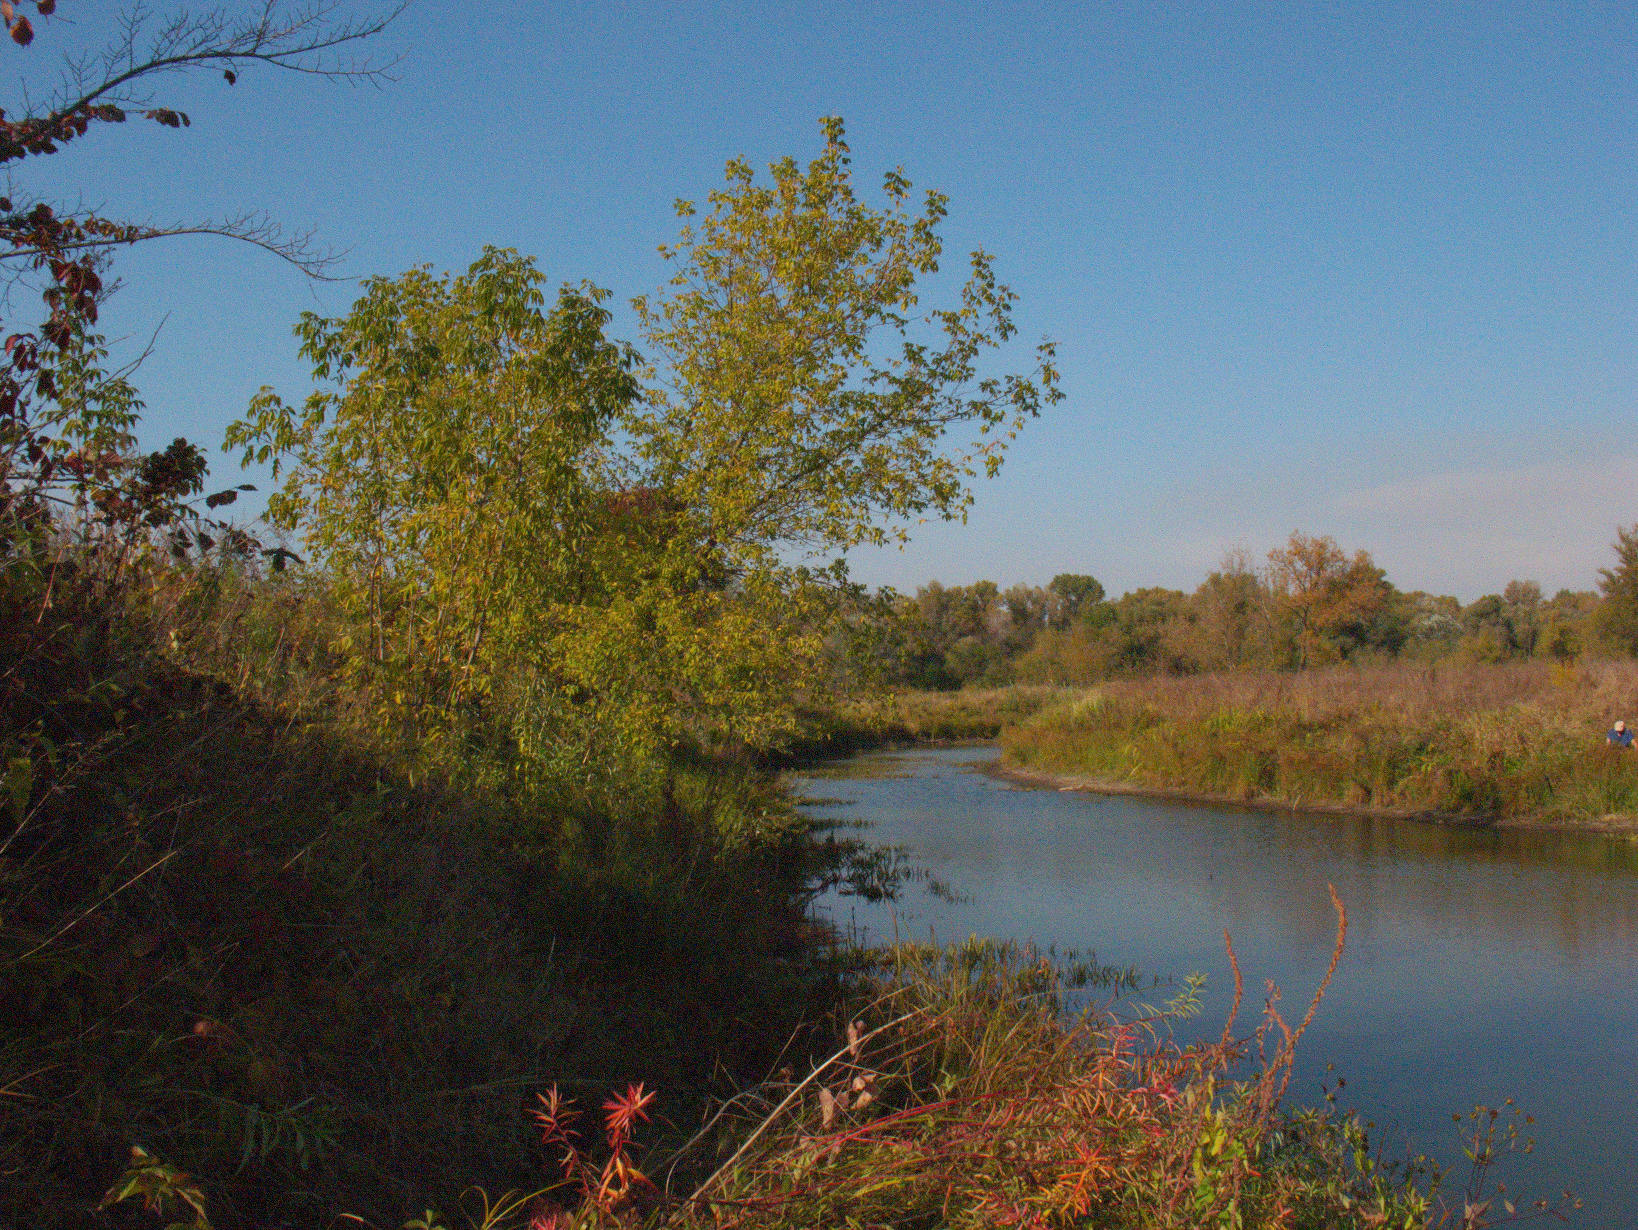
\includegraphics[width=0.80\linewidth]{chast-gorodki/cherto/star-rechka-CRW_4023.jpg}

\textit{Залив Старая Речка осенью 2014 года.} 
\end{center}

\begin{center}
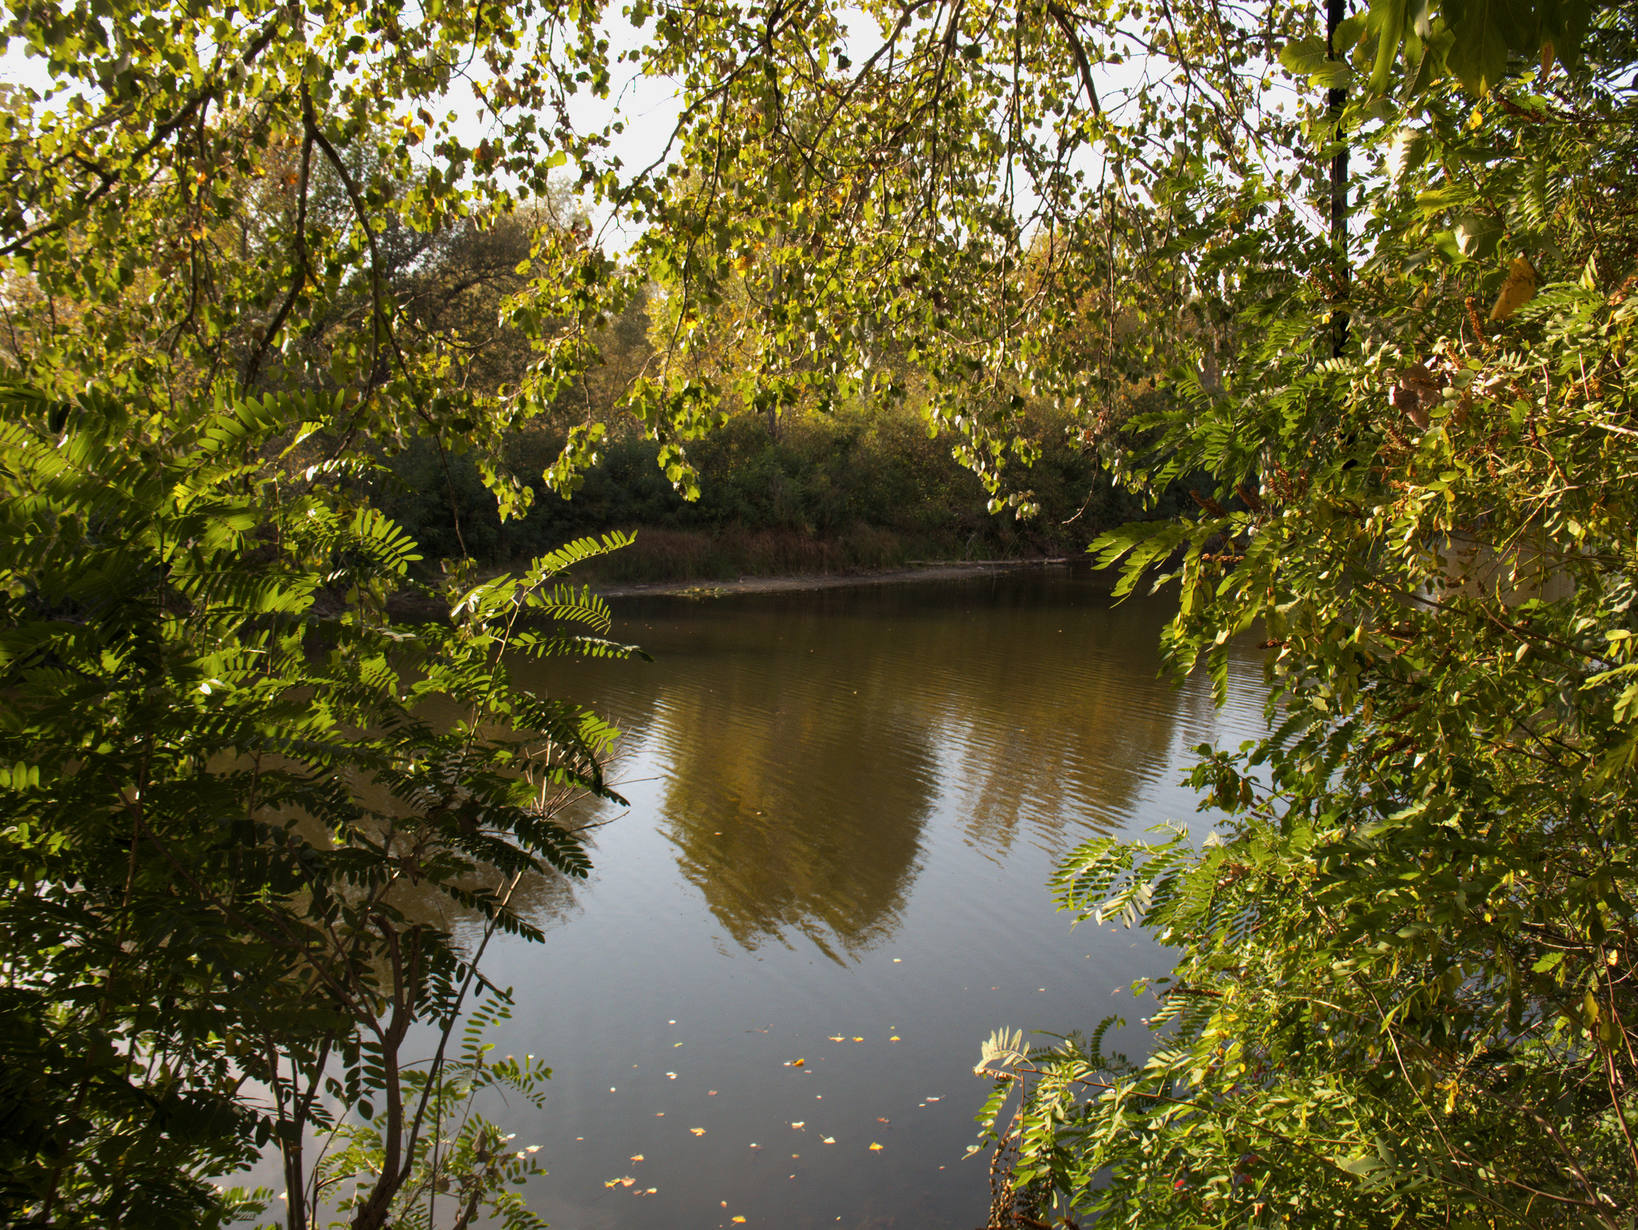
\includegraphics[width=0.80\linewidth]{chast-gorodki/cherto/kin-CRW_4003.jpg}

\textit{Кинище, осенью 2014 года.} 
\end{center}

\newpage

Лучшие по ракурсу фотографии оказались совсем испорченными, кроме того я забыл сфоткать Малое Кинище. Старая Речка меня удивила высокими берегами. Не по всей длине, а кое-где, поверхность суши острова там выше, чем поверхность воды, метра на четыре. Уровень воды от дна я не мерял. Местами этот залив почти прерывается заиленными отмелями, но чуть пройдешь, и видишь уже внушительную луговую реку. Хотя тоже, ощущение рукотворности этого водоема. Слишком правильный.

Предполагаю, что «речкой Бобровней» на карте Сноевского подписано Кинище, возможно купно со Старой Речкой – их в самом деле, по вытянутым очертаниями, можно принять за части рек, и последнее в прошлом не противоречит истине.

Вот карта 2014 года, на которой я примерно и угловато обрисовал север Муромца и его содержимое. Сопоставив план Сноевского и мою карту, можно примерно вычислить, где находилось городище с плана.

\begin{center}
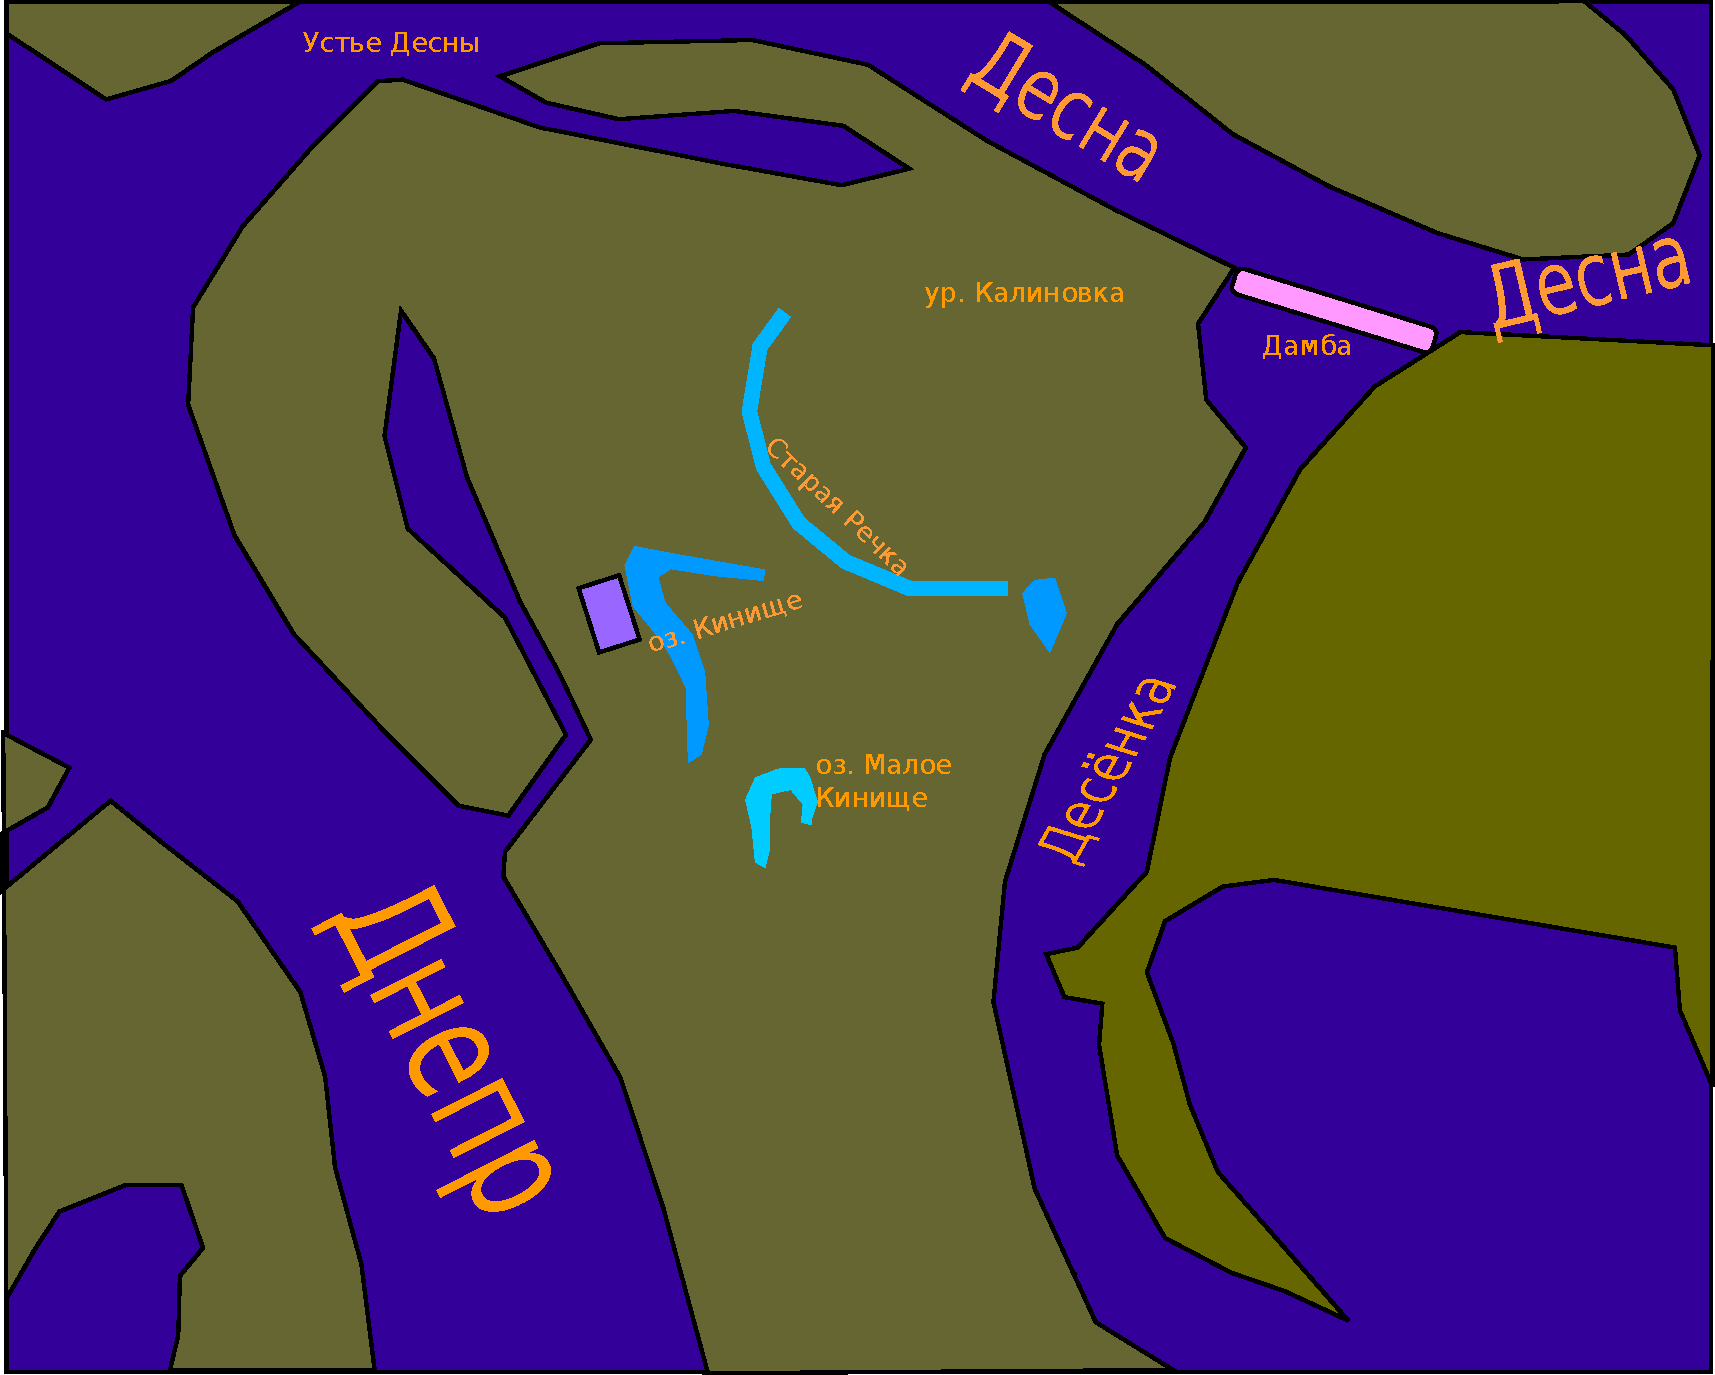
\includegraphics[width=\linewidth]{chast-gorodki/cherto/mur-nord-map.pdf}
\end{center}

Названия урочищ на Муромце даны по плану Днепра 1914 года.

Розовая палочка – дамба, отделяющая исток Десенки от Десны. Фиолетовый прямоугольник – заброшенная база отдыха «Березка» возле озера Кинища. У него тоже крутые, высокие берега.

Надутый залив в нижней правой части – до 1877 года там было село Троещина, а западнее его остров, обмываемый Черторыей-Десенкой. В тридцатых годах 20 века, непосредственно севернее места той старой Троещины в Черторыю впадал рукав Десны, отделявшийся от заболоченной ныне ее старицы\footnote{50°32'26"N 30°33'52"E}, хотя на плане Шуберта середины 19 там видны лишь причудливые озера. Впрочем, к северу и северо-восток от Троещины план Шуберта сильно теряет точность и ошибается в расстояниях.

%Десна на протяжении лет петляла в тех краях немыслимо, и сопоставляя карты, видны моментальные снимки местности, по коим трудно проследить ее плавное развитие. В таком-то году – картина одна, в другом – совершенно иная.
  
Залив возле устья Десны – это, наверное, бывший рукав, причем относительно современный, ибо на карте лоций 1914 года его нет. Берега залива укреплены камнями, над восточной частью нависают старые, с густой прической ивы. В чистой темной воде покоятся лилии.

Старая Речка дугой огибает местность, в 1914 году подписанную как урочище Калиновка. Судя по карте Шуберта, еще в середине 19 века это был остров в самом верховьи Десенки, со всех сторон омываемый деснянской водой. Согласно Шуберту же, Кинище впадало в рукав Днепра ниже устья Десны, чуть южнее широты современного залива Верблюд.

Вообще на Муромце различалось много урочищ. Там где нынче непосредственно парк – урочища Еловатое да Нижнее Заречье. В восточной части острова – озеро Глубокое, переходящее в болото. Северней его было меньшее озеро Грузные Долины, а восточнее – Муравка. Озером «Большая Бобровня» на старых картах иногда подписывали верховье Небышевки. Вот откуда, думаю, ошибка на планах современных. К западной части Глубокого почти примыкало Щитецкое, Щиток – канал, соединяющийся с Небышевкой.

На Муромце были сенокосы села Троещино, что до 1877 года, когда случилось большое половодье, располагалось севернее Выгуровщины, на левом берегу Черторыи.

Затем жители Троещино переселились восточней, вглубь материка. Прежнее место стало «Старой Троещиной», новое – «Новой Троещиной» и просто Троещиной. В начале 21 века примерно в месте первого теперь – залив Доманя и восточнее – крайняя к заливу часть коттеджного городка «Деснянский».

А вот отмеченное на картах южнее залива урочище «Старое село» хоть и близко к прежнему месту Троещино, однако только близко.

При Литве с Польшей, сенокосами да пастбищами Муромца и Труханова владели то доминикане, то шляхтич Осецкий, коему принадлежал большой остров Осецкий севернее Муромца, по другую сторону Десны. На карте Днепра за 18 век, село Осещина (где ныне и Осецкий остров) лежит, однако, на том же берегу Десны, что и Троещина, а значит устье Десны было севернее нынешнего.

Осенью 2014-го я, при своих тогдашних представлениях, пробовал найти городище на Муромце («А» по плану Сноевского), предполагая в нем один из Городков, а именно – упомянутый в летописи за 1151 год.

Ученым известно некое городище на этом острове, но точных координат у меня нет. В «Своде памятников истории и культуры Украины», книге первой, части второй, под номером 298 внесено «Муромец, городище, 12-13 век». Про него сказано, что находится в северо-восточной части острова Муромец. Открыл археолог Михаил Сагайдак в 1982 году, исследовал в 1990-м. Оно же, возможно, и есть «городище А» на плане Сноевского.

Статья из «Свода» сообщает, что археологическое раскопки не проводились, однако некие «материалы исследований» хранятся в Институте Археологии НАН Украины. Указана форма городища – круглая, площадь – три с половиной гектара. В заметке говорится, перевожу с украинского на русский:

\begin{quotation}
Оборонные валы вокруг городища едва заметны, с юго-восточной стороны обнаружены остатки внешнего рва. Ширина вала и рва около 4-5 метров. Вход в городище находился с юга. Близ него обнаружены остатки ровчака, который выходил к протоке, омывающей остров. Возможно, в древнерусское время это был канал, которым из Днепра можно было подплыть к городищу.
\end{quotation}

Невесть почему городище отождествляется наукой с загородным двором Юрия Долгорукого – «Раем» (про который в летописи сказано лишь, что он был «за Днепром», и помимо Рая существует еще прочтение – Саморай) или с местом пребывания князя Михаила Всеволодича в 1241 году «под Киевом на острове». Да мало ли под Киевом островов?

Найдены некие бугры на Муромце. Не более, ведь раскопки не проводились. По виду – городище, остатки населенного укрепления. И в этих буграх подозревают «Рай» или место временного проживания другого князя.

Какие предпосылки это подозревать? Никаких. Разве что «Городец» застолблен наукой возле Выгуровщины, на берегу озера Гнилуши, а стало быть, по академической науке, любое другое городище это конечно же остатки Рая.

Площадь 3,5 гектара. Как это вообразить? Сколько это метров в разные стороны? Городище сверху похоже на круг. Можно вычислить, что диаметр такого его будет 211 метров. Заложив руки за спину, прошагаем 211 метр. Вот какая длина у городища по справочным сведениям.

Я много ездил по Муромцу на велике в поисках какого-либо городища. У меня была карта Сноевского, которой я тогда всецело доверял, и понимание, где искать – на берегу озера Кинища, однако я не знал площади – 3,5 гектара. Искал просто любое городище, не обязательно большое. Хотя бы остатки чего-то. И я нашел.

У самого южного конца Кинища\footnote{\textasciitilde{}50°32'16.23"N 30°32'34.88"E} есть заросшая кустами и деревьями местность, с довольно правильной формы невысоким, длиной с автобус «Икарус», горбом. Что там дальше, я выяснить не сумел. Часть этой местности огорожена забором, и с велосипедом далеко в кусты я пробраться не мог. Выбраться туда пешком пока не получается.

Покажу неудачно запечатленный в 2014 году бугор, принятый мною за часть городища. Хорошо ли видно?

\begin{center}
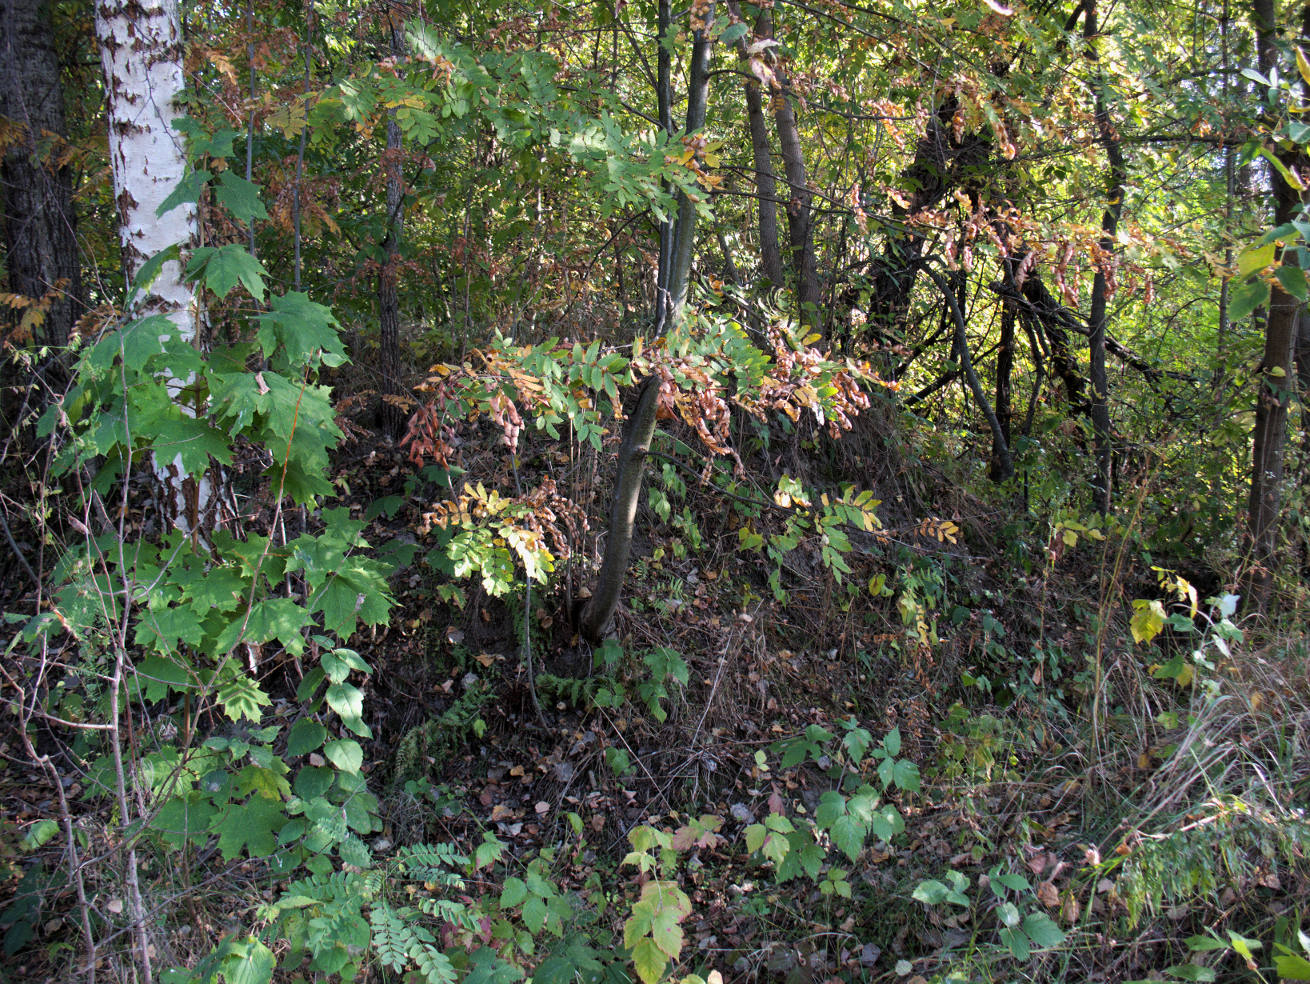
\includegraphics[width=\linewidth]{chast-gorodki/cherto/mur-CRW_4031.jpg}
\end{center}

Еще мне показалось, что там русло Кинища искусственно перегорожено, завалено чем-то.

Учитывая, что я осмотрел все окрестности, городище возможно только в этом месте. Оно вычислено по карте Сноевского и катанию просторами Муромца. Если никаких других бугров правильной формы я не заметил, и рассчитывал найти таковые именно возле Кинища, то значит, это городище «А» и есть.

Однако можем ли мы соотнести с ним городище, найденное Сагайдаком? Нельзя на это ответить, не ведая, где последнее. Может, на Муромце существовало два городища в северной части острова.

Казалось бы, любое городище именно там – след замечательного пункта для охраны водных подходов к Киеву, а заодно взымания налогов. Оттуда, небольшая крепость обозревала бы сразу несколько рек, и будучи соединена с ними каналами... Но это поверхностные рассуждения.
Мы даже не знаем, где было устье Десны в летописные времена.

Что за городище на Муромце, что там могло остаться после бесчисленных половодий, заливавших остров? Боюсь, иного ответа, кроме фотографии заросшего горба, не будет.

%Другое такое удобное место, где на виду Десна и исток Десенки – на углу материка, обозначено у Сноевского буквой «В», вот только исток Десенки там – 19 века, а несколько прежде он был не западнее «В», но восточнее!

Ниже Муромца, между Днепром и Черторыей, находится Труханов остров. Прежде остров\'а разделялись проливом Пробитцем. Запруженный до упора, он виден еще на картах начала 20 века, на широте Куренёвского трамвайного парка, теперь это депо имени Красина. Да, с тех самых пор депо не переезжало.

Дореволюционный Труханов остров – ресторан с парком «Эрмитаж», пароходные мастерские, яхт-клуб\footnote{Командором его в последнем десятилетии 19 века был гидролог Николай Максимович, стоявший у основания клуба.}, пляж, базар, поселок. Много лет жили там самосёлами работники пароходства, но потом, в 1907 году дума разрешила селиться всем. Слободка узаконилась и расширилась. Сюда провели телефон, построили училище, рядом, в 1910-м – по проекту архитектора Евгения Федоровича Ермакова каменную церковь святой Елизаветы, названную в честь не столько святой, сколько генерал-губернаторши Елизаветы Треповой.

Часть земли Труханова острова с 1885-го арендовало пароходное общество. Оно владело пароходами! И тут же, на Трухановом, чинило оные в мастерских. Вокруг и вырос поселок, обслуживая пароходство.

Главой пароходного общества был Давид Марголин. В 1908 году, в связи с 50-летием Общества, он построил на острове здание школы с ремесленным отделением, на 150 учеников. Марголин хотел передать школу городу, но с условием быть почетным попечителем, и дабы школа носила его имя. «Давида Марголина?!» – встрепенулись в городской думе\footnote{Ранее, до принятия закона о запрете евреям быть депутатами, Марголин  заседал в думе и в 1890 году «провёл» там создание Общества киевской городской железной дороги, иначе говоря трамвая. И сам это общество возглавил. Акционерами же стали Струве и Лазарь Бродский. Позже Марголин завел собственную трамвайную линию на Демиевке.}. И начали тянуть волынку. Тогда Марголин передал школу Киевскому благотворительному обществу, «Сулимовке»\footnote{Оно располагалось в усадьбе Сулимовке в центре города. Сохранилось основное здание по адресу Лютеранская, 16, и здание приюта – Круглоуниверситетская, 5.}. Во главе общества в то время стояла Елизавета Сергеевна Трепова, жена киевского генерал-губернатора Федора Федоровича Трепова. Школу разрешили открыть, что и случилось год спустя.

Вероятно, условием к благополучному исходу дела, выдвинутым со стороны Треповой Марголину, было устроение на острове также церкви.

По проектам епархиального архитектора Евгения Ермакова (1868-1914) в Киеве возведено немало зданий, относящихся к церкви. Различные школы, училища, внутренние постройки монастырей – ризницы, библиотеки, кельи, гостиницы, просвирни, а также несколько церквей. Много его работ в Лавре и Выдубичах. Он же спроектировал Кокоревские беседки на Владимирской горке и Андреевском спуске, да вероятно приложил руку к Дому Ричарда.

О Марголине (1850-1918?). Родом из Пинска, восемнадцатилетним переселился в Киев. Занимался разного рода торговлей, в 1875 году служил управляющим на одном из кирпичных заводов Якова Бернера. Сахарозаводчик. Основатель и руководитель 2-го общества пароходства по рекам Днепровско-Припятского водного бассейна, позже возглавил Соединенные общества пароходства по Днепру, монополиста речных перевозок. Добыча нефти на Кавказе и Каспии. 

Сведения о Марголине после 1917 года противоречивы. То ли умер 30 июля 1918 года, то ли эмигрировал, как его сын Арнольд, ставший при Скоропадском сенатором и генеральным судьей, а при Петлюре вице-министром иностранных дел.

Противоположна судьба внука Марголина, Михаила Владимировича (1906-1975). Когда семья в 1918-м бежала из Киева, он потерялся и остался в городе. Прибился к бойцам Красной армии, в 1919 году уехал на Кавказ к матери, которая была учителем в школе-коммуне. Работал конюхом, плавал на шхуне матросом. Пятнадцатилетнего Михаила Марголина назначили комендантом штаба Частей особого назначения в Хосте, затем – командующим взводом. 

В 1924 году, восемнадцатилетний, получил ранение в голову и ослеп. Вернулся в Киев, в инвалидный городок, что находился при Лавре. Затем Михаил Марголин переехал в Харьков, на курсы слепых массажистов. В 26-м отправился в Москву, стал инструктором по стрелковому оружию при ОСОАВИАХИМ. Наощупь освоил механику, начал сборку своих моделей оружия – винтовок, пистолетов, мелкокалиберных пулеметов. Для общения с чертежниками использовал макеты из воска, пластилина, дерева, пластмассы. С 38-го работал в различных конструкторских бюро, в 58-м стал главой КБ при научно-исследовательской стрелковой станции ДОСААФ, одновременно продолжая разработку спортивного оружия.

Наиболее известен Марголин своим пистолетом МЦ – «Марголина Целевой», выпускавшимся «в подлиннике» с 1946 до 1979 года. Его используют до сих пор в спортивных соревнованиях, обучению стрельбе. С девяностых годов в ход пошел усовершенствованный вариант – «Марго». Пистолет системы Марголина был придуман им в трамвае, по ходу на работу. Просто в голове возникло устройство пистолета, все его составляющие. Уже через несколько дней были готовы опытные образцы.

Сам слепой изобретатель научился стрелять на звук.

Да, но довольно о Марголиных, вернемся на Труханов!

Дореволюционный поселок сосредоточился на части острова между Днепром и Матвеевским заливом. Матвеевский (ранее Старик) получил название от некогда находящегося тут дачного имения богатого акушера, профессора медицины, ректора Университета святого Владимира, Александра Павловича Матвеева (1816-1882). На заседаниях ученого совета он спал, а по окончании вставал и приглашал всех к себе домой обедать.

На Тарасовской улице, в доме с ухоженным декоративным садом, принимал гостей барином, окружив себя волчатами и медведями, чьих родителей он, страстный охотник, убил. Питая расположение университетских преподавателей, Матвеев отталкивал своим поведением студентов. Один даже ударил его камнем по голове.

На западном берегу острова, напротив Почтовой площади Подола, был небольшой залив, а за ним – пустырь, далее Днепровская набережная, и между нею и озерцом – церковь и училище. Знаменитый парк Эрмитаж находился чуть южнее широты Почтовой, на улице Остёрской, западным краем примыкая к берегу Днепра. Вообще дореволюционный Труханов – это сетка прямых улиц: Полтавской, Харьковской, Остёрской, Екатериновской, Черниговской, да переулков Переднего и Киевского. 

Между парком и церковью были пароходные мастерские. К юго-востоку от Эрмитажа располагалась Запорожская площадь, рядом с нею – огромный нефтяной бак.

В начале 20 века остров безуспешно, якобы по просьбе жителей, пытались переименовать в Алексеевский, то бишь царевича Алексея, наследника престола – это название, покантовавшись на картах, умерло вместе с царской властью.

В 1910-1912 годах в северной части Труханова, напротив Воскресенской слободки, а точнее – нижней части озера Радунки, Киевское общество любителей природы построило биологическую станцию, на деньги профессора Университета Святого Владимира Кеппена, который умер в 1910-м, завещав деньги и оборудование обществу. Станция занималась изучением пресноводной флоры и фауны, после несколько раз переезжала. Ныне это гидрологическая станция «Киев», на западном берегу Гидропарка, метрах в ста с лишком южнее моста метро.

Самым знаменитым местом Труханова был Эрмитаж. Он возник не на пустом месте. С некоторых пор, еще пару веков назад, киевляне завели моду отдыхать на природе. Расстилали там ковры, разные подстилки, да поглощали пищу. Поныне так!

\newpage
\vspace*{\fill}
%\begin{center}
%\includegraphics[width=\linewidth]{chast-gorodki/cherto/tru-19x1.jpg}
%\end{center}

\begin{center}
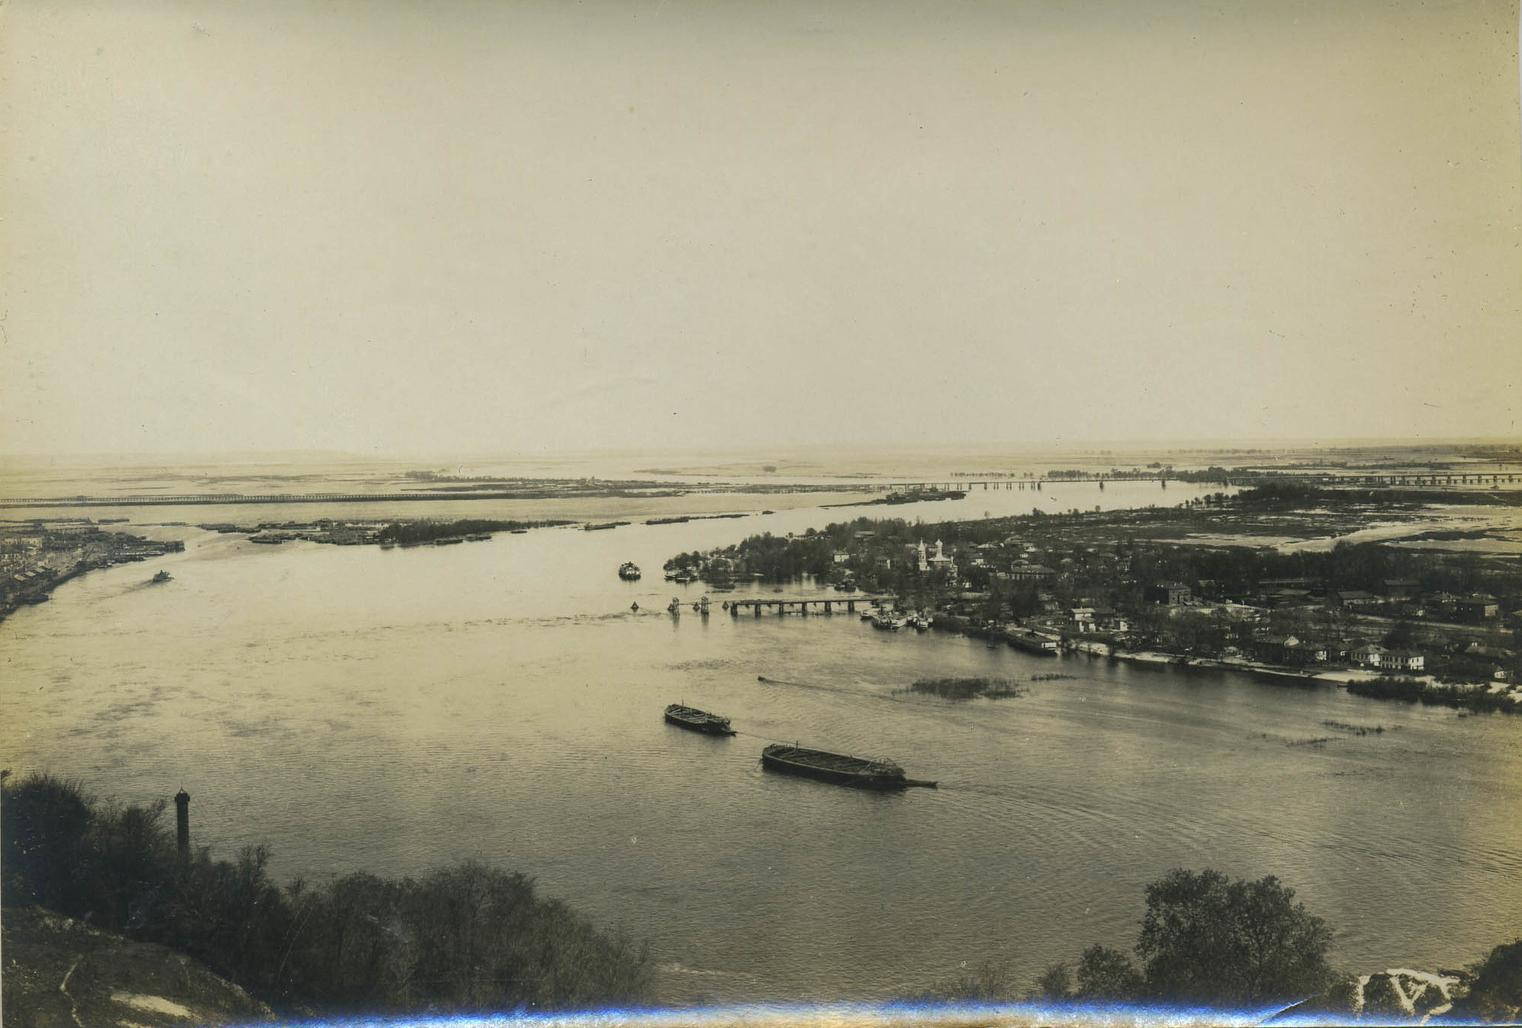
\includegraphics[width=\linewidth]{chast-gorodki/cherto/truhanov-s-gory.jpg}

\textit{Вид на Труханов с правого берега. Дореволюционное фото.}
\end{center}


\begin{center}
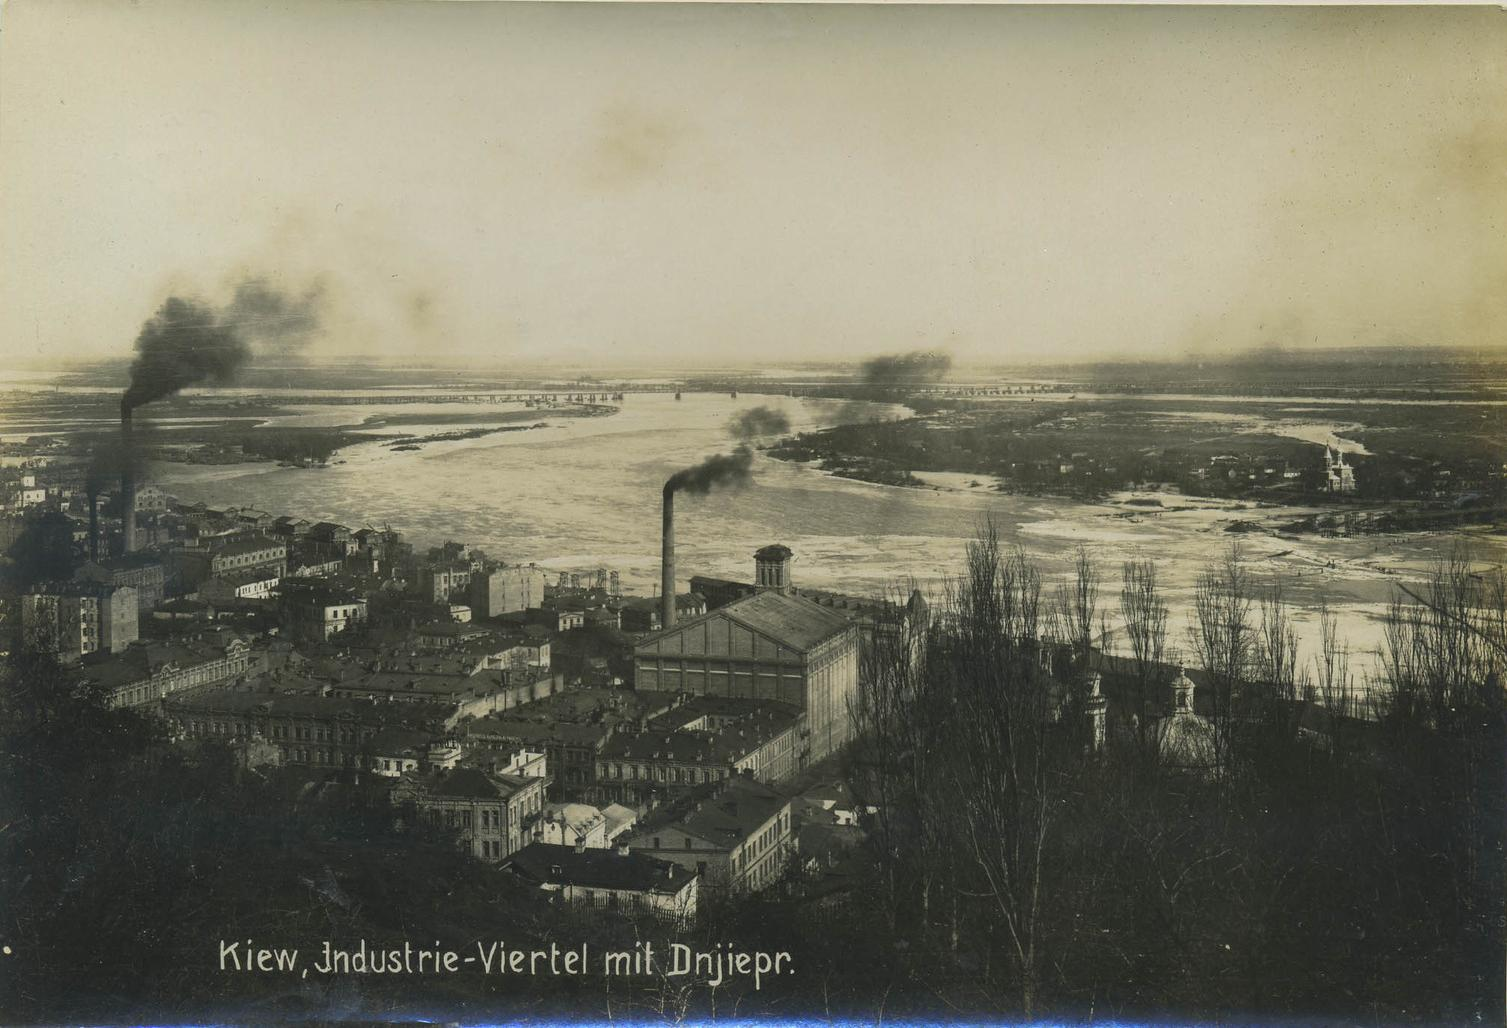
\includegraphics[width=\linewidth]{chast-gorodki/cherto/tru-19x2.jpg}

\textit{Вид на Подол и Труханов, дореволюционный снимок.}
\end{center}
\vspace*{\fill}
\newpage

%\begin{center}
%\includegraphics[width=\linewidth]{chast-gorodki/cherto/truh01.png}

%\textit{Улица на Труханове, дореволюционный снимок.}
%\end{center}


%\begin{center}
%\includegraphics[width=\linewidth]{chast-gorodki/cherto/truh-dor002.jpg}

%\textit{Разлив на Труханове, дореволюционный снимок.}
%\end{center}

%\newpage

\vspace*{\fill}

\begin{center}
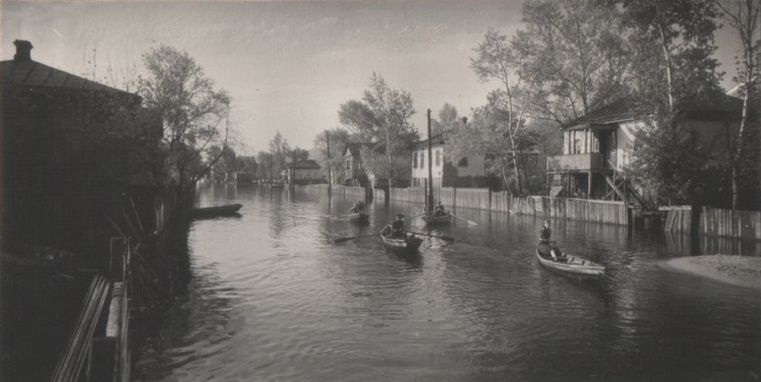
\includegraphics[width=\linewidth]{chast-gorodki/cherto/1941-truh-razl-1.jpg}

\textit{1941 год. Разлив на Труханове.}
\end{center}


\begin{center}
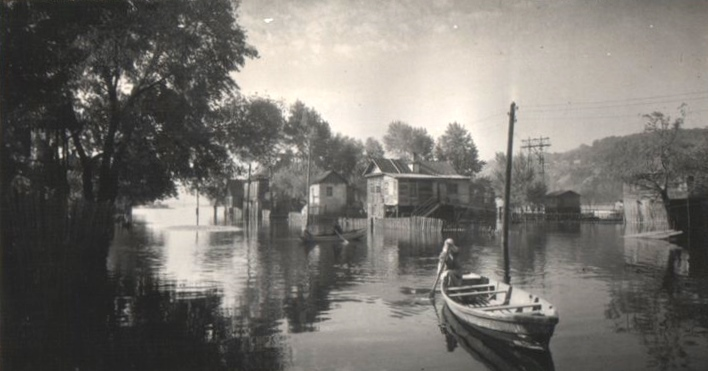
\includegraphics[width=\linewidth]{chast-gorodki/cherto/1941-truh-razl-2.jpg}

\textit{1941 год. Разлив на Труханове.}
\end{center}

\vspace*{\fill}

\newpage



И вот на Труханов переправлялись лодками, тащили с собой самовары, всякую снедь, выпивку.

В 1872 году, житель острова, владелец лодочной переправы, купец Адам Доминикович Гинтовт поставил на Трухановом закусочную, чтобы кормить любителей пикников. Начал с чая, пива и раков, потом отстроился, увеличил меню. Заведение Гинтовта быстро обросло темным элементом. Пьяные драки, насилие – и никакой помощи жертвам. Корреспондент «Киевлянина» писал:

\begin{quotation}
Я был свидетелем следующих сцен: две компании пьяных мужчин снесли и вбросили в лодки двух обезображенных молодых женщин, одетых лишь в изорванные рубахи. Женщины эти кричали: «Где мои деньги? Где моя кофта?» Но крик их был в полном смысле гласом вопиющих в пустыне: они немедленно были увезены от берега. Хозяйка трактира, стоя на берегу, смотрела на эту сцену с полнейшим хладнокровием.
\end{quotation}

Гинтовт продолжал богатеть и расширяться. На месте прежней наливайки соорудил ресторан «Эрмитаж» с парком, где был летний театр. Играло два оркестра. Пели шансоньетки и куплетисты. Рядом грохотали вагонетки «американских горок». При «Эрмитаже» была даже собственная электростанция.
 
Для массового завоза посетителей на остров предприимчивый литовец пустил два маленьких парохода. Гинтовт и раньше переправлял народ на Труханов, однако лодками, беря по пять копеек. В августе 1883 года, в бурю во время переправы утонуло несколько человек, и Гинтовт решил обезопаситься, вначале арендовав один пароход, а затем присовокупив и второй. Газета «Киевлянин» тогда сообщала:

\begin{quotation}
В воскресенье, около 8 часов вечера, разразилась в Киеве гроза с сильным ливнем и бурей. Вследствие праздничного дня на Днепре была масса лодок с пассажирами, частью переправлявшихся на Труханов остров, а частью катавшихся вверх и вниз по Днепру. Во время бури лодка, управляемая одним гребцом, опрокинулась возле пароходной пристани. В лодке находилось 16 пассажиров.

На страшные крики о помощи люди бросились спасать утопающих. Спасено 11, остальные 5 пошли ко дну. Многие ищут своих родных, которые отправились «за Днепр», но до сих пор еще не возвращались. У лодочной пристани ниже купален также толпится масса народа. По сведениям, полученным подольским полицейским участком, у Чертороя погибло до 30 человек.
\end{quotation}

Пароходы оказались выгоднее лодок, ибо городская управа предписала впредь иметь на лодке двух гребцов и рулевого – против единственного лодочника на лодку, как было у Гинтовта. К тому же ввели ограничение на количество пассажиров в одной лодке. А пароходы позволяли обойти количественное ограничение. Вози сколько хочешь, нету закона против. Билет на пароход стоил 10-15 копеек в зависимости от класса, да за вход в парк Гинтовт брал по 20.

Прежней публике новые затеи оказались не по карману. На другом берегу Матвеевского залива был ресторан «Босфор» от пароходства, да и на правобережной горе белела ракушка летнего театра в Парке купеческого собрания. А в Предмостной слободке гудел подобный «Эрмитажу», но меньшего масштаба, ресторан с парком «Венеция». Ближайшие соперники. «Эрмитаж» стал Гинтовту в убыток и разорил его. К 1912 году остался только одноименный парк, без кафешантана.

Но увеселительное заведение гибло не сразу, а постепенно. Окруженный конкурентами, в 1888 году Гинтовт затеял долгосрочную аренду островной земли, сроком на 12 лет. «Эрмитаж» был летним. Долговременная аренда позволила бы Гинтовту спокойно выстроить зимние сооружения, чтобы увеселять круглый год. Городские власти выдвинули условия – поднятие арендной платы, благоустройство острова (что включало высадку 3000 деревьев, укрепление берега), и передачу всех строений городу через 12 лет.

Гинтовт отказался. Аренду выставили на торги, где победил всё же Гинтовт, причем условия были на сей раз более выгодные. Правда, срок аренды сократили вдвое.

Приблизительно в это время на Труханове развернул деятельность Давид Марголин со своим Пароходным обществом. Установил цистерны с горючим. Просачиваясь, оно начало уничтожать раков, которых много лет тут же и ловили для ресторана Гинтовта. Пришлось закупать раков на Житнем рынке, но посетители воротили носом. Не то! Гинтовт сдал Владимиру Аммунсу часть земли под «Русские горки». Не раками, так горками, народ потянули в «Эрмитаж».

Желая, чтобы ресторан шагал в ногу со временем, отвечал запросам современной публики, Гинтовт назначил управляющим своего сына Цезаря. Кто, как не он, знает вкусы молодежи? Под чутким руководством Цезаря посетителей принялись обсчитывать на баснословные деньги, десятки рублей.

Тогда Гинтовт решил сделать ставку на, как бы нынче сказали, «кризисного менеджера» – из самой Америки! Его звали Вольдемар Саламонский. Через полгода Саламонского выдворили за пределы России – еще до устройства на работу у Гинтовта американец своей деятельностью привлек к себе внимание полиции.

В 1896 году Гинтовт не нашел средств внести очередную плату за аренду. Затем снова. Власти приказали ему снести постройки ресторана с острова и вернуть землю городу. Гинтовт возражал. Зря.

Ресторан с парком отобрали и выставили на торги.  Разоренный Гинтовт с семьей перебрался на Никольскую слободку, где следы его теряются.

Помимо Эрмитажа, севернее, был еще парк яхт-клуба – к его узким аллеям в плодовом саду вела каменная лестница о пяти ступенях, по сторонам с невысокими колоннами. Вазы с цветами венчали их. На полукруглой площадке стояла пушка.

В советское время, до сороковых годов, часть улиц Труханова переименовали, возникли и новые, например Чертов переулок, Черторыйская улица – граничащие, впрочем, с Матвеевским заливом.

Школа получила номер 101\footnote{Последний ее директор, Борис Петрович Толстой, лейтенант НКВД, погиб в застенках Гестапо, арестованный по доносу завуча этой же школы.}, появился детский сад, медицинская амбулатория, летний кинотеатр – где выступал Утёсов, стадион, милицейский участок. В 1939 году на острове постоянно проживало 1096 человек, однако всего там обитало около семи тысяч в нескольких сотнях деревянных домов. На Труханове был только один автомобиль – пожарный. Ездили на великах, а в Киев лодками.

Немцы во время Великой Отечественной уничтожили поселок.
\vspace*{\fill}
\begin{center}
\includegraphics[width=\linewidth]{chast-gorodki/cherto/\myimgprefix truh.jpg}

\textit{На берегу заметна ограда с воротами Эрмитажа, за нею павильоны, потом задняя ограда.}
\end{center}
\vspace*{\fill}
\newpage
\vspace*{\fill}

Дореволюционные снимки Труханова. Школа и училище, вид с разных сторон:

\begin{center}
\includegraphics[width=\linewidth]{chast-gorodki/cherto/truhanov-сerk-01.jpg}
\end{center}

\begin{center}
\includegraphics[width=\linewidth]{chast-gorodki/cherto/truhanov-сerk-02.jpg}
\end{center}

\vspace*{\fill}
\newpage
\vspace*{\fill}
\begin{center}
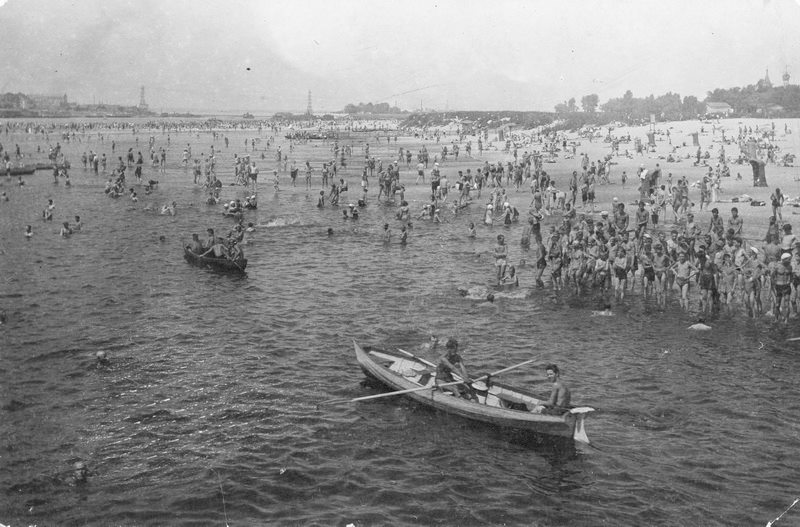
\includegraphics[width=\linewidth]{chast-gorodki/cherto/tru01.jpg}

\textit{1930-е. Пляж на Труханове.}
\end{center}


\begin{center}
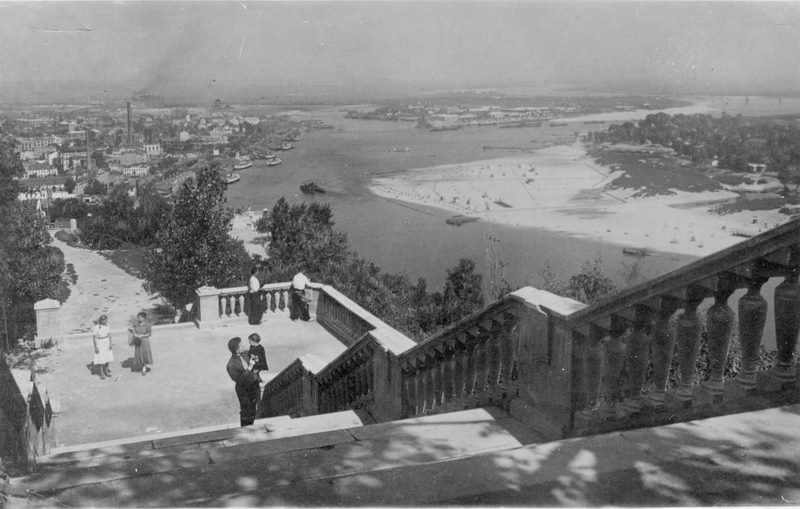
\includegraphics[width=\linewidth]{chast-gorodki/cherto/tru02.jpg}

\textit{1930-е. Вид на Труханов с Пролетарского сада.}
\end{center}

\vspace*{\fill}
\newpage
\vspace*{\fill}
\begin{center}
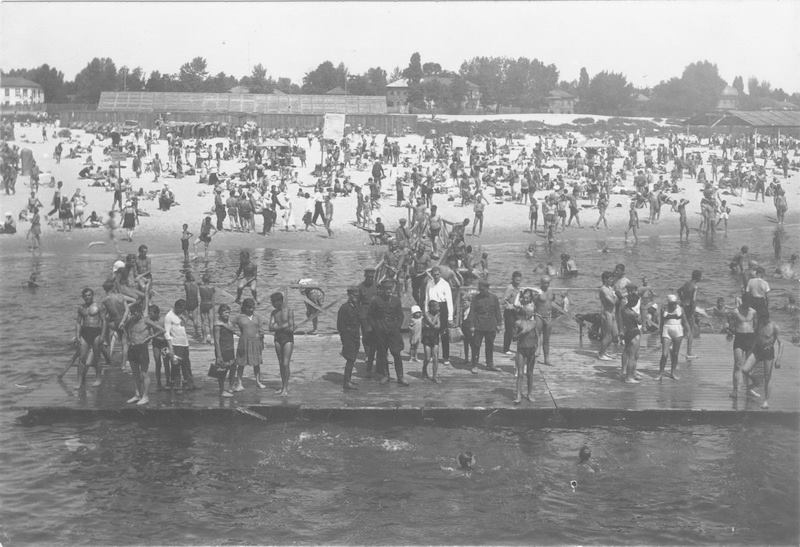
\includegraphics[width=\linewidth]{chast-gorodki/cherto/tru03.jpg}

\textit{1930-е. Пляж на Труханове.}
\end{center}

\begin{center}
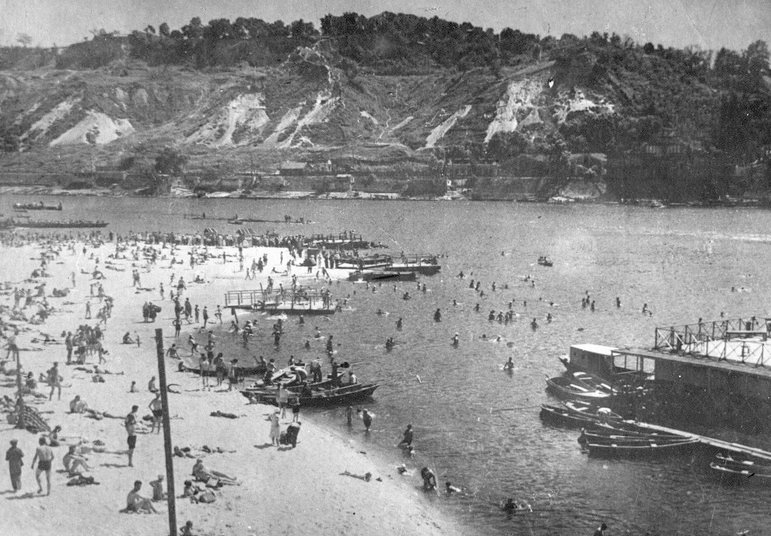
\includegraphics[width=\linewidth]{chast-gorodki/cherto/tru04.jpg}

\textit{1930-е. Вид с Труханова на правый берег.}
\end{center}
\vspace*{\fill}
\newpage

На фотографиях 1930-х, да и конца пятидесятых, заметно, что Днепр на протяженности вдоль Труханова (эдак по стадион «Динамо») был много \'уже, и пляж простирался почти до теперешней середины реки. Возвышение же берега Труханова начиналось поодаль этой громадной отмели. Конечно, во время весенних разливов вода поджимала, и между постройками да рекой оставалась узкая полоса, а то и вовсе весь остров погружался в воду. Долгим динозавровым хребтом над нею торчали деревья, домики.

\begin{center}
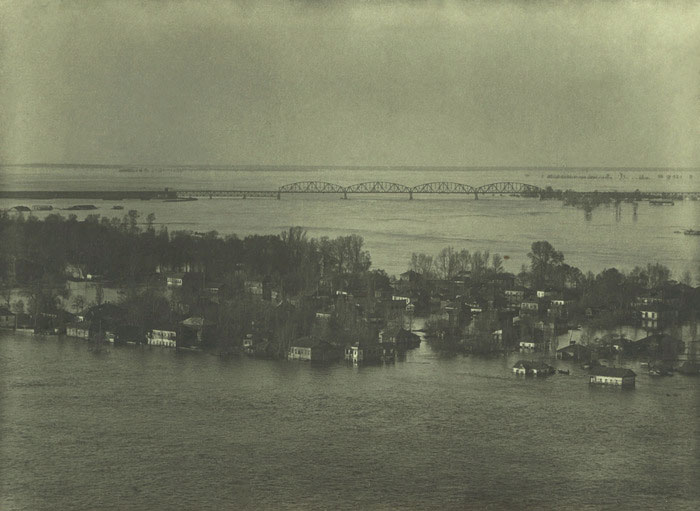
\includegraphics[width=\linewidth]{chast-gorodki/cherto/tru05.jpg}
\end{center}

На остров, как прежде, переправлялись на лодках. Только в 1957-м перебросили Пешеходный мост. Еще в 1964 году ширина Днепра в том месте была такова, что первая у острова опора стояла посреди пляжа, вторая – рядом с самим берегом, а вокруг третьей находилась обширная отмель, островок.

В пятидесятые годы на Трухановом работала парашютная вышка, в шестидесятых аттракцион прикрыли, но вышка продолжала стоять, и ныне снова используется по назначению.

\begin{center}
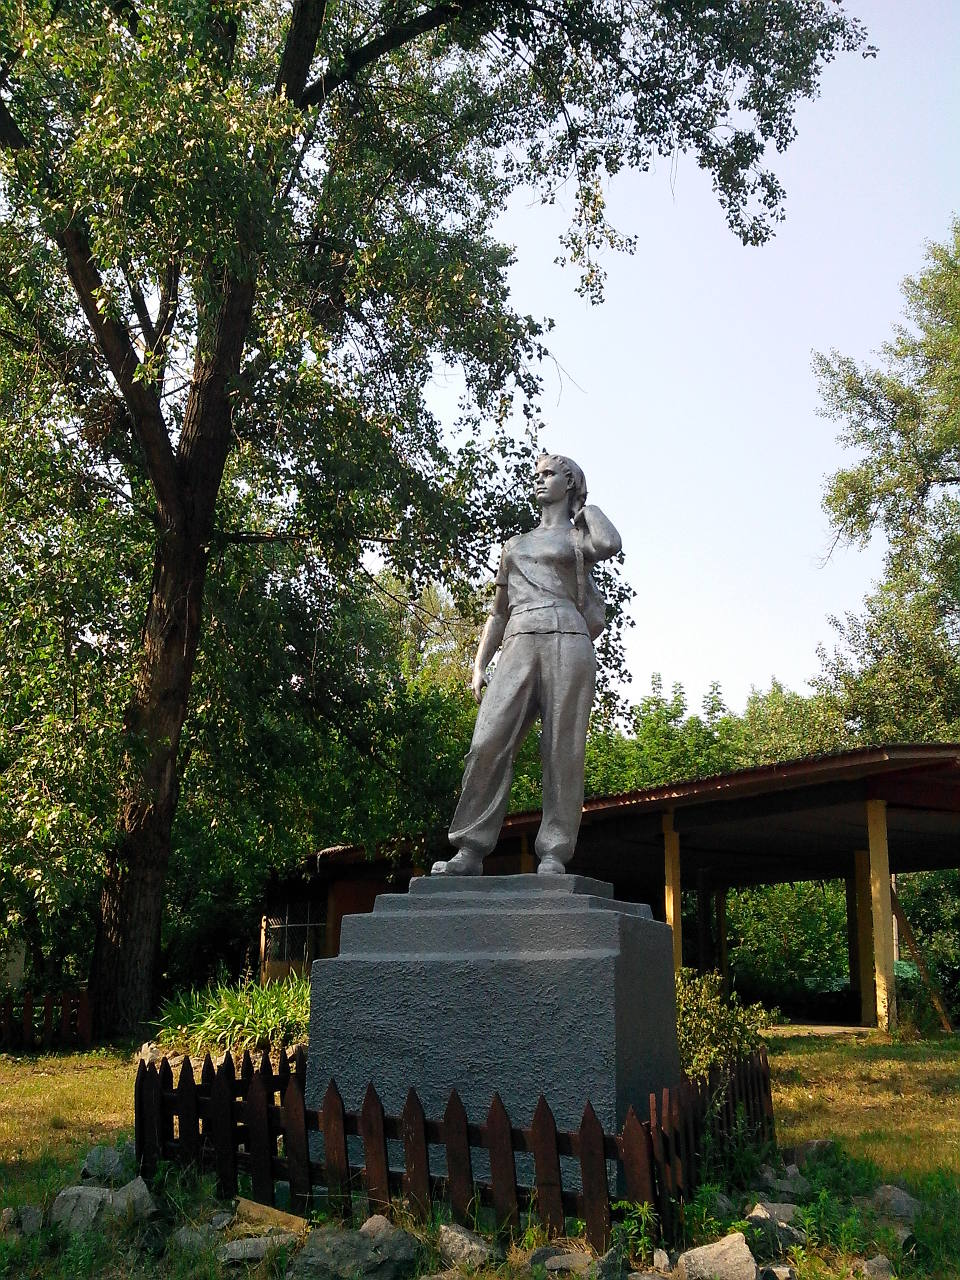
\includegraphics[width=\linewidth]{chast-gorodki/cherto/s_tru_IMG_20130628_162249.jpg}

\textit{Советская статуя. Снимок 2013 года.}
\end{center}

Со старых времен сохранилось немного. Ресторан, бугры на месте развалин церкви и училища, да была статуя спортивной девушки – ее разбили осенью 2015-го.

На острове натыкано различных спортивных баз, есть заброшенные советские базы отдыха и пионерлагеря. Было здорово – зеленый остров посреди города, на нем отдыхали в домиках люди. Всё это продолжалось до развала Союза. А теперь – мертвые помещения, кое-где раскуроченные, а где и уцелевшие. Висит стенгазета на стене, гипсовый Ленин машет рукой в приветствии, а фонарь на бетонном столбе кто-то особо меткий расшиб камнем, и дорожки из плит всё больше затягиваются травой.

А в лесу, в месте, где до войны был дом 15 на Полтавской улице, есть могильная ограда с холмиком\footnote{50°27'51"N 30°32'10"E}. Висит табличка:         

\begin{quotation}
Перепеча Меланья Фоминична и ее внук Анатолий. Их убили у порога родного дома немецко-фашист\-ские захватчики при сожжении рабочего поселка «Труханов остров» в сентябре м-це 1943 г.
\end{quotation}

Всего тогда погибло 86 человек – учтённых. Зная о наступлении наших войск, немцы уничтожали островные посёлки, чтобы Красная армия не воспользовалась ими как плацдармом. Был приказ всем оставить слободки, и если гитлеровцы кого замечали – расстреливали на месте.

В шестидесятые, бывшие жители посёлка основали землячество «Труханов Остров». На День Победы и 27 сентября они приходят к особому, 1989 года, памятнику на острове – это вернувшийся с фронта солдат, он стоит над лодкой с проломленным днищем. Солдат вернулся, а нет родного поселка. Вся прежняя жизнь кончилась. И он застыл.

У землячества был свой музей в пионерском лагере «Ленинец», что просуществовал до нового века. Музей оттуда выставили, экспонаты хранятся у бывшей подпольщицы Галины Хоменчук. Во время войны около двух десятков совсем молодых трухановцев стали подпольщиками – устраивали диверсии на верфи, которую немцы прибрали к рукам, разбрасывали листовки. Эти-то прежние подпольщики и решили сходиться в памятные дни на острове. Поначалу сие вызывало недоумение у милиции. «Чего вы тут собираетесь?» – спрашивали стражи порядка у людей с орденами Героев Советского Союза.% Один из подпольщиков, на 2014 год – глава трухановского землячества, капитан-лейтенант в отставке Евгений Леонидович Тамаров.

%После войны на опустошенном Труханове высадили деревья. Люди перебирались туда ради пляжа. Понемногу остров оживал. Построили на уцелевшем основании от дореволюционного топливного бака круглый ресторан «Відпочинок» – до сих пор стоит там заброшенный. По пути от него и до Бабьего озера (бывшая часть Матвеевского залива, выглядит как буква Y, около него растут дикие гладиолусы), под сенью огромной ивы возникло «Монте-Карло» – оборудованное парой десятков столиков место сбора доминошников и преферансистов.

После войны, остров являл выжженную пустыню с развалинами домов. В 1944 году вышло постановление поселок не восстанавливать. В 1947-м люди высадили деревья. Остров не должен был застыть страшным кладбищем. 

Люди перебирались туда ради пляжа. Понемногу остров оживал. Построили на уцелевшем основании от дореволюционного топливного бака круглый ресторан «Відпочинок» – до сих пор стоит там заброшенный. По пути от него и до Бабьего озера (бывшая часть Матвеевского залива, выглядит как буква Y, около него растут дикие гладиолусы), под сенью огромной ивы возникло «Монте-Карло» – оборудованное парой десятков столиков место сбора доминошников и преферансистов.

Постепенно Труханов стал парком и напряженно остается им поныне. Люди идут сюда Пешеходным мостом, и едут на машинах по шоссе через Муромец, с Московского моста. Наливайки, снаряды для качания мускулов, пёстрые пляжи и строго огражденные участки с табличками «Частная собственность».

Конечно, можно свернуть в лес, подальше, еще сохранились места. Там растут сосны, высокая трава. Но природы становится всё меньше, ее теснят оглушающие рок-концерты, дискотеки, жилые деревни для шведских фанатов. А по северной части острова проложили Подольско-Воскресенский мост, подмявший и часть Русановских садов на противоположном берегу Черторыи.

%Черторыя, двигаясь руслом своим на юг, размывала, меняла существующие там сложные структуры заток Днепра и Десенки с Радункой, повлияв таким образом сначала на Труханов остров, затем на Гидропарк. И заливы, что относились сначала к Днепру, подчинились в итоге Черторые.

\chapter{Тельбин}

Поговорим теперь про озеро Долобское, пролив Долбичку, озеро Тельбин и связь всего этого с летописной речкой Золочей.

Эту головоломку решают уже несколько сотен лет, рассматривая задачу лишь на узком отрезке времени и пространства, поэтому приходят к противоречивым выводам, которые легко поколебать, добавив в рассуждения упущенный из виду довод.

В нашем же повествовании местом действия послужит весь левый берег, временем действия – сотни лет, а действующие лица будут появляться по мере надобности.

Современный пролив Долбичка. Черторыя около Труханова острова разделяется на два рукава. Один идет прямо, другой выгибается к востоку. Остров между рукавами на современных картах называют Долобецким (в конце 19 века его северная половина была отдельным островом Кутом). Туда перебираются небольшим мостом с Гидропарка. А пляж нудистов «Долбичка» лежит напротив, на юге Труханова, тоже омываемый проливом Долбичкой, с юго-восточной стороны. Берег пляжа в первой половине 20 века был частью суши Гидропарка.

Прямое русло Долбички и служит сейчас основным руслом Черторыи, ибо идет прямо, по виду естественно продолжая реку, в то время как восточный рукав выглядит второстепенным. Но если следовать взглядом на юг, то именно восточный рукав продолжается в качестве Русановского пролива, а вот Долбичка через Венецианский пролив упирается в северный берег Гидропарка, напротив пляжа нудистов.

От прежней Долбички остается только название, протяженность между широтами, да направление течения, и то – с середины 19 века оно сменилось с юго-западного на южное. Веками русло плясало, извиваясь по местности, на нее влияли как природные, так и человеческие силы – рылись каналы, сооружались запруды. И если только за прошедшие полтора столетия русло изменилось совершенно, то как заглянуть в более далекое прошлое?
%Русло Долбички начала 21 века пересекается по координатам с руслом Долбички середины 19 века только на двух коротких отрезках. На нее влияли как природные, так и человеческие силы – рылись каналы, сооружались запруды. 

А ведь считается, что «на месте Долбички» раньше находилось Долобецкое озеро, упоминаемое в летописях и старинных земельных документах. Да где на месте, на каком? Русло Долбички какого времени принимать за «это место»?

В летописи единожды упомянуто «озеро Дулебское» и несколько раз просто урочище «Долобьске». Там князья иногда сходились на совещания. Например, в 1103 и 1111 годах Святополк и Владимир встречаются в шатре «на Долобьске», причем не указано, озеро это или такая местность. А в 1101 году князья-братья собираются на Золочи.

Долобское озеро вписано в Жалованную грамоту Киевского воеводы Юрия Монтовтовича Пустынно-Никола\-евскому монастырю, 4 июля 1508 года:

\begin{quotation}
Я, Юрьи Михайлович Монтовтовича, воевода Киевский, державца Черниговский и Любецкий. Били нам челом старци з монастыря Святого Николы Пустыньского, штобыхмо придали на тот монастырь и церкви Святого Николы озеро, на имя Долобеск, и с устьем в острове в Туханове.
\end{quotation}

Вообще сведения о Долобском озере скудны. В путеводителе по Киеву конца 19 века впрочем говорится о Долобском как об озере на Труханове, и что оно летом часто пересыхает. Но возможно, сочинитель принимал за Долобское озеро другой водоем.

Долобское озеро (а озером тогда могли называть и залив) и Золоча возникают в летописи при описании попыток Гюрги (Юрия Долгорукого) в 1151 году форсировать Днепр, чтобы выбить Изяслава из Киева. Наиболее подробно сие описано в Ипатьевской летописи:

\begin{quotation}
И поиде Гюрги к Киеву\footnote{Гюрги плыл на лодках по Десне из Городка Остёрского.} и сташа в Родуни, и придоша Половци диции\footnote{Дикие.} мнози Дюргеви в помочь; и Изяславу же блюдущу вбрести в Днепр, и тако начаша ся бити по Днепру у насадех\footnote{Насад – речное судно, у которого основа долбленая, а борта набиты, досками.} от Кыева оли и до устья Десны, ови ис Киева в насадех выездяху биться, а они ис товар; и тако бьяхутся крепко, не могоша бо что успети противу Киеву. 

Бе бо исхитрил Изяслав лодьи дивно: беша бо в них гребци невидимо, токмо весла видити, а человек бяшет не видити; бяхуть бо лодьи покрыты досками, и борци стояще горе в бронях\footnote{Бойцы стояли наверху лодок, одетые в броню.} и стреляюще, а корменика два беста, един на носе, а другый на корме, а может хотяхуть, тамо поидяхуть, не обращающе лодий\footnote{Два рулевых, на носу и корме, что позволило плыть в любую сторону и поворачивать, не делая разворот лодьи.}.

И оттоле Гюрги сгадав с Володимером с Давыдовичем, и с Святославом Олговичем, и с Всеволодичем Святославом, и с Половци, и хотящим вниз пойти к Витечевьскому броду, не смеющим же им пустити лодии мимо Киев, но пустиша е во озеро Дулебское и оттоле волочиша е берегом в Золотчу, по Золотчи же внидоша во Днепр лодье их; Половци же Гюргеви идяху по лугу.
\end{quotation}

Гюрги в лодьях из Десны смог «сташа в Родуни». Про Родунь мы будем рассуждать в других главах, пока примем, что это некое урочище близ устья Десны. Однако мы не знаем, где было устье Десны в летописное время, посему передвижения Гюрги начинают проясняться только у Труханова острова.

На помощь Гюрги, к Родуни, прибывают дикие Половцы. Но Изяслав, стерегущий (блюдущий) брод через Днепр, не дает Гюрги и Половцам переправиться. Изяслав сражается в насадах, а у Гюрги есть лодьи и военный обоз, повозки. Фронт разворачивается по Днепру от Киева и до устья Десны. Изяслав и дополнительные насады из Киева мешают Гюрги.

%Поскольку речь идет о седой старине, уместно предположить, что устье Десны могло быть где угодно – а хоть бы Десной считалось и русло в протяженности современных Десенки и Черторыи, и тогда устье Десны вполне подходило к Труханову острову, а не к Муромцу, как нынче.

%Вот незадача. Для простоты рассуждений поступим как делают ученые. Примем, без всяких доводов, что устье Десны лежало примерно на той же широте, что и сейчас. Я вообще дальше буду с натяжкой делать некоторые утверждения, допуская, что русла с летописных времен изменились не сильно – что, конечно же, маловероятно.

Гюрги держит совет с Володимером Давыдовичем, Святославом Олговичем, Святославом Всеволодичем, и Половцами. Здесь перебраться на правый берег не получается, что делать? Искать другое место. Решают пробиваться вниз к Витичевьскому броду\footnote{Возле селения Витачов (Вытачов) близ Триполья. У южной околицы Витачова, над Днепром, есть древнее городище, возможно то самое, о котором пишет Константин Багрянородный в «Об управлении империей», говоря о судоходстве и том, что Росы от крепости Киоавы «двигаясь по реке Днепр, они спускаются в Витичеву, которая является крепостью-пактиотом Росов».}. Брод нужен для обоза Половцев. По какой-то причине Гюрги не смог сразу плыть вниз по Днепру, и пускает свои лодьи в озеро Дулебское, оттуда волочит их по берегу в Золочу, а из Золочи лодьями выплывает в Днепр. Половцы же едут лугом, параллельно лодьям.

Будучи в Днепре, Гюрги вводит свои лодьи в Дулебское озеро. Значит, оно было заливом, соединенным с Днепром!

Совершенно верно. А рядом, западнее, протекал рукав Днепра, ставший потом Матвеевским заливом. Во время Гюрги это был, думаю, основной рукав Днепра, где и разворачивалось сражение. Черторыя не упомянута – вероятно, она еще не существовала.

%И привычная нам Черторыя в то время просто не существовала и не доходила руслом к Долобскому «озеру», а точнее заливу.

Затем Гюрги перетаскивает лодьи по суше из Дулебского озера в Золочу, а из Золочи уже выплывает в Днепр, ниже по течению. Следовательно, Золоча впадала в Днепр, а между нею и Дулебским озером была суша. Это также означает, что никакой другой воды в то описываемое время между Золочей и Дулебским озером не было. Важно!

Летописец очень тщательно передает последовательность перемещений войск. В Дулебское озеро из Днепра лодьи не перетаскивали, а из Дулебского в Золочу – понадобилось волочить по суше. Это однозначно говорит о том, что Дулебское – залив, а Золоча – река или другой залив, тоже соединенный с Днепром. И между Дулебским заливом и Золочей был отрезок суши. Выстраивается цепочка с севера на юг: Днепр – Дулебское – суша – Золоча – Днепр.

%Отсюда следует, что в рассматриваемой местности не просто не существовало Черторыи, но и другого рукава Десны, если только под Десной не подразумевалось русло Черторыи. Иначе, будь отдельный рукав, Гюрги в своих перемещениях из Долобского в Золочу неизбежно должен был его пересечь. Этого не случилось.

%Если бы какое-то русло, рукав Десны, будь то Десенка или Черторыя, протекало так (от Десны до Гидропарка) при Гюрги, то Гюрги в своих перемещениях из Долобского в Золочу неизбежно должен был пересечь Черторыю. Этого не случилось.


%Значит, Черторыя тогда вероятно не существовала как поименованный водоток от Десны, и уж точно не доходила до широты озера Долобского. Ибо позже таки дошла и течет теперь по месту озера Долобского как пролив Долбичка.

%Либо значит, что Десной таки считалось русло в протяженности нынешней Черторыи, однако по ряду причин мне неудобно так думать.

Попади мы в летописное прошлое, то очень удивились бы, увидав, как всё было на деле. Но судить можем лишь по более новым картам.

Рассмотрим кусок плана 1750 года. Верхняя сторона карты – запад.

\begin{center}
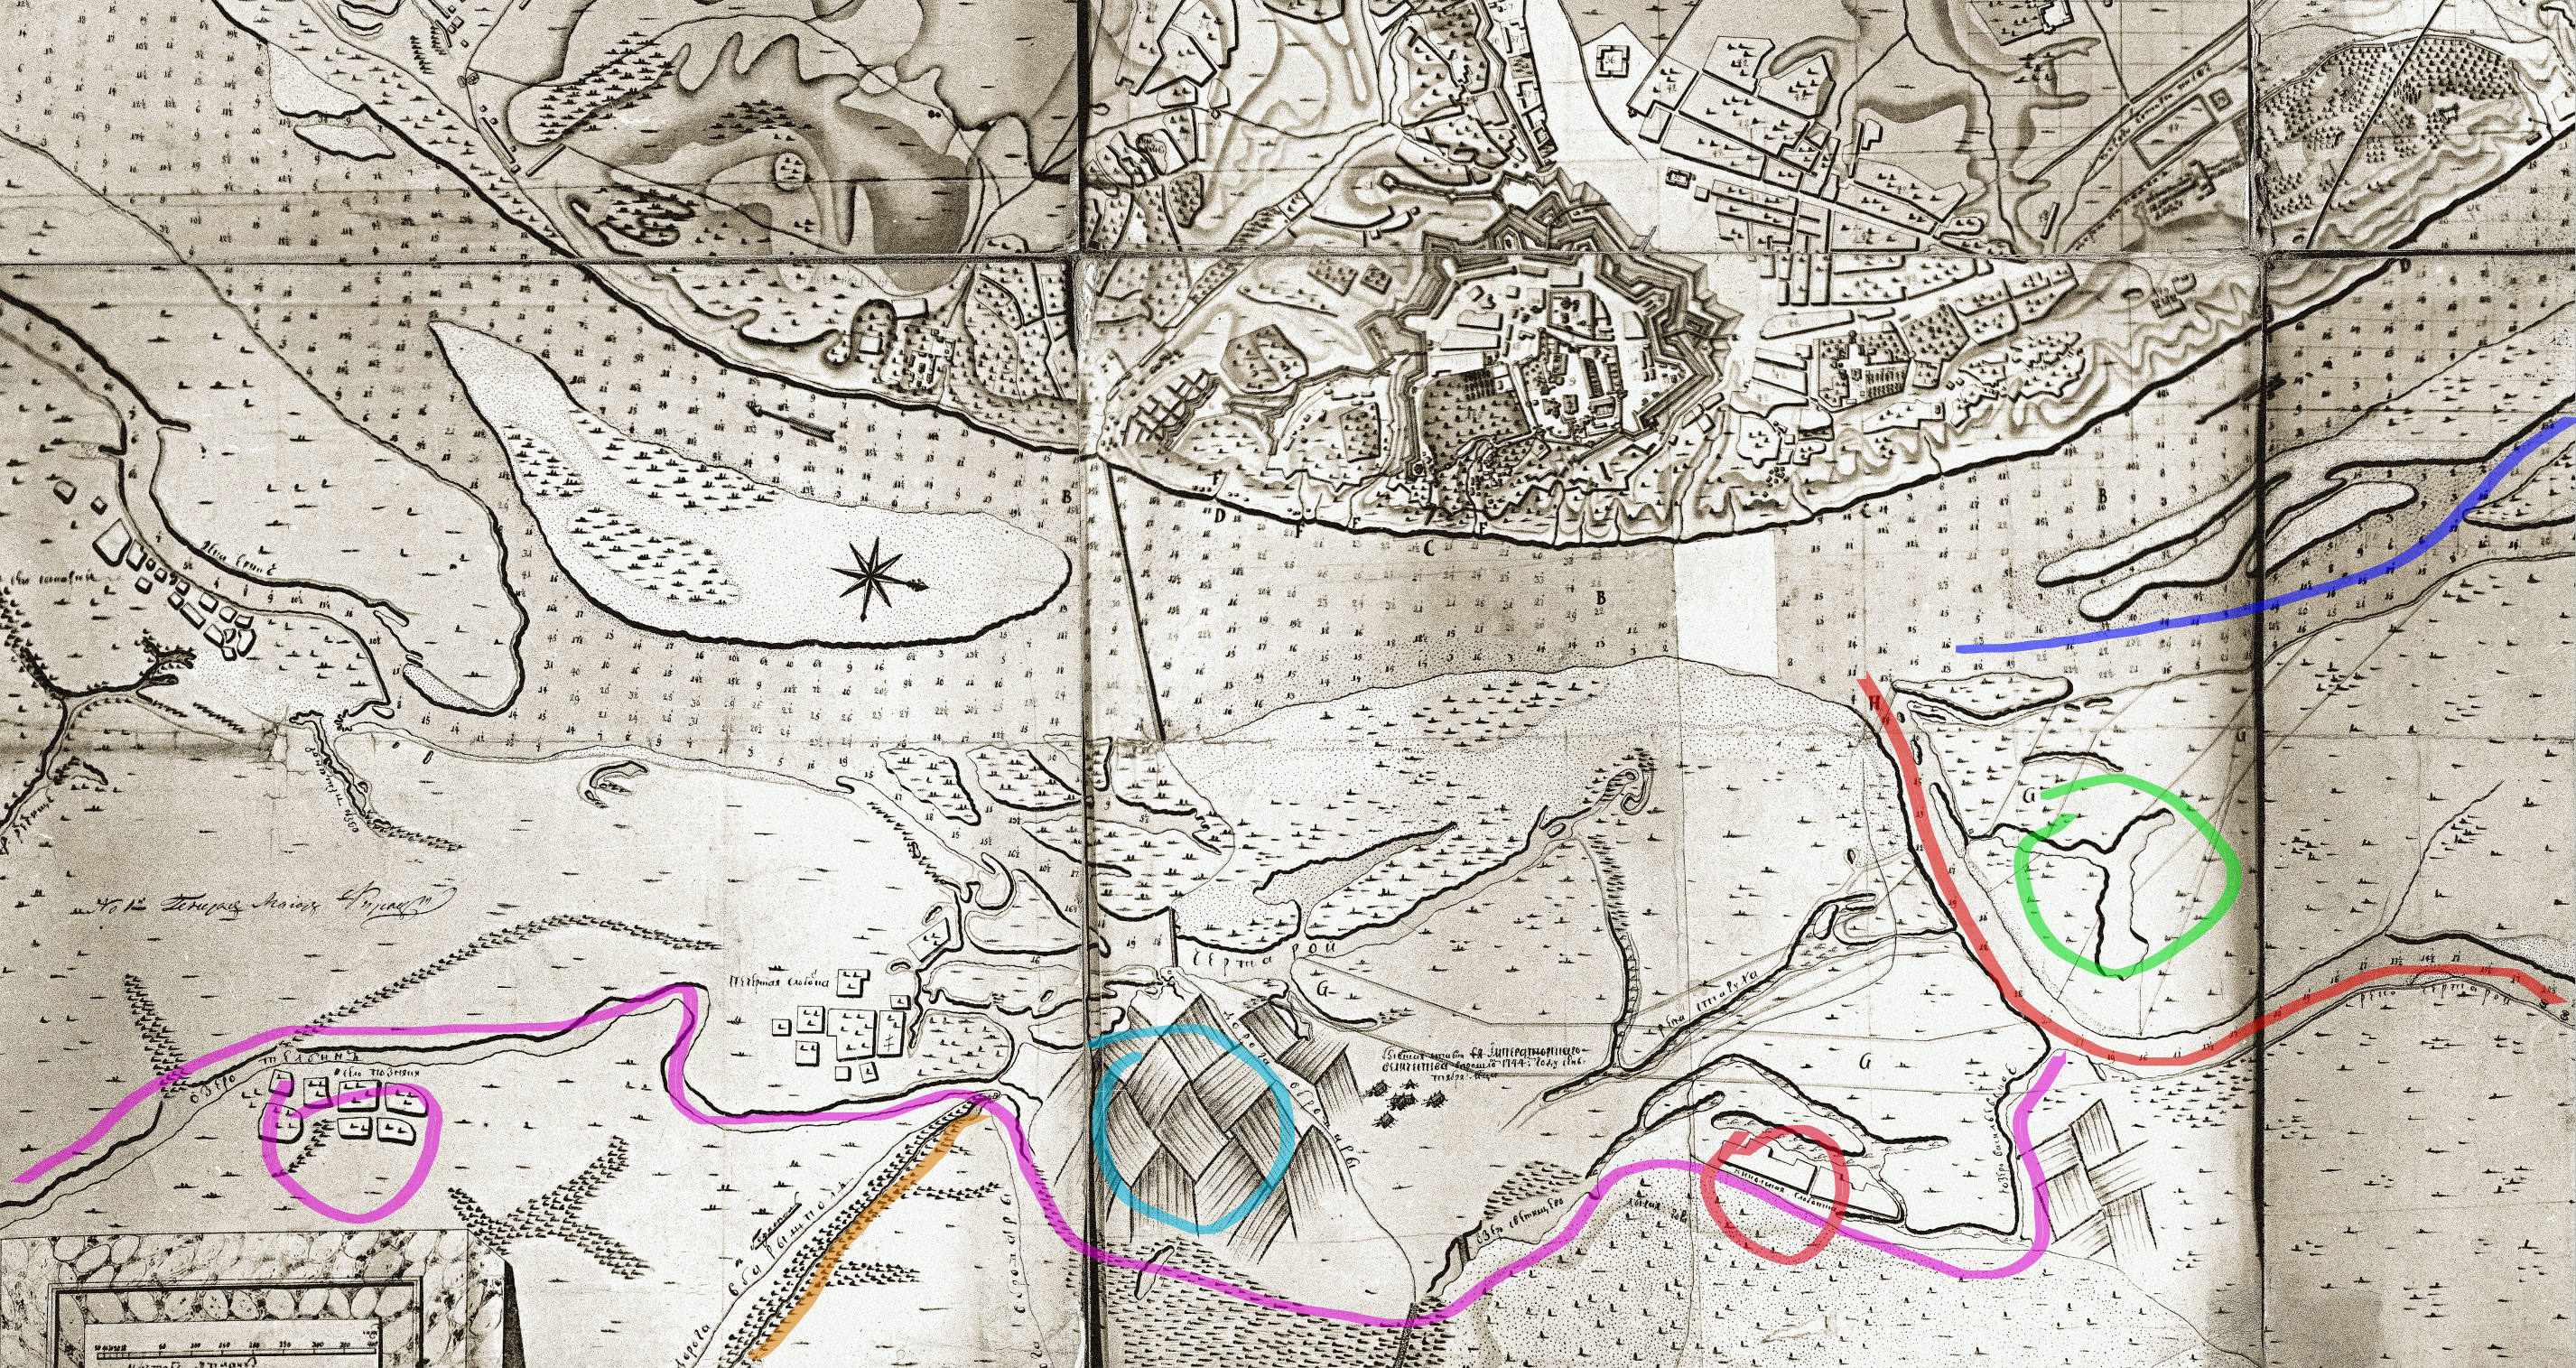
\includegraphics[width=\linewidth]{chast-gorodki/terbin/1750-telbin-new.jpg}
\end{center}

%На куске плане 1750 года видно положение, где основное русло Черторыи (подпись «река Чертарой», правее, не поместилась) сворачивает к Днепру на широте эдак моста Метро, а южнее, хотя и подписан там залив «Чертарой», очевидно, что это не продолжение Черторыи, но порождение Днепра. Рассмотрим внимательно. Верхняя сторона карты – запад.

Подобный шестеренке многоугольник посередине вверху – крепость вокруг Лавры. Вертикальная линия через Днепр в первой трети картинки – переправа около Наводничей. Это главные ориентиры.

Салатовым кружочком я обвел Долобское озеро. Точнее, на картах 19 века в том месте находится водоем других очертаний, подписанный как Долобское озеро.

Красный кружок – Никольская слободка.

Голубой кружок – вспаханные поля, где ныне Русановка.

Малиновый кружок – село Позняки.

Красной линией показано основное русло Черторыи (подпись на карте, «река Чертарой» – есть, однако не поместилась на скопированный мною кусок). Слева (южнее) от него теперь мост Метро. 

Еще южнее лежит «река Старуха», а потом снова «Чертарой», южнее Никольской слободки. По виду он похож, скорее, на старицу Днепра. Через него перекинут мост от дороги с Наводницкого моста. 

Синяя черта – рукав Днепра, ставший потом Матвеевской затокой.

Оранжевая черта – речка Дарница.

Малиновая линия – так я предполагаю некогда единое русло-продолжение Долобецкого залива. В районе Никольской слободки я отвел его чуть ниже настоящих водоемов. На 1750 год русло включает в себя озеро Васильевское, Русановское, Светищево, и болото переходящее в речку Тельбин.
 
Что получается? 

Если Гюрги в 1151 года плыл по «синему» руслу Днепра, то на восток (на карте – вниз) от этого русла Днепра лежал залив, ставший потом Долобским озером. В его северную часть можно было зайти из основного русла. Чем Гюрги и воспользоваться, чтоб укрыться от неприятеля.

Как далеко простирался залив в сторону Золочи?

Долобское озеро на карте 1750 года словно пересекается «красным» руслом Черторыи. А что к востоку, на карте – ниже этого пересечения? А там продолжается сей прежний Долобский залив. Пока Черторыя не перерубила залив надвое, либо разделение произошло по другой причине, это было единое русло. И дальше оно продолжается на юг, в обход современной Русановки с востока. 

На Светищево и это болото да истоки озера Тельбин (образца середины 19 века) почти совершенно накладывается нынешний Русановский канал.

Печерская слободка на этом плане то же, что на других – Кухмистерская слободка. Она лежала по западному берегу Тельбина, между ним и Днепром. А на восток от Тельбина позже возник хутор Зательбин Березняк. Позже на месте обоих селений был построен жилой район Березняки.

% с Печерской слободкой на карте петрушка получается. Дореволюционные карты так именуют два разных поселения. Одни карты обозначают так местность, известную ныне как Гидропарк. Другие же Гидропарк называют Предмостной слободкой, а Печерской слободкой – хутор Зательбин Березняк, он же Березник, где позже возник жилой массив Березняки.

%Дореволюционные планы частенько величают Предмостную Слободку – Печерской. 

%На карте же 1750 года, умозрительно, находясь примерно на широтах между Наводничами и Выдубицким монастырем, эта Печерская слободка однозначно сопоставляется с Кухмистерской с тех же позднейших карт.

На плане Сноевского, «речка Тельбин» – а ныне от нее известен отрезок в образе озера Тельбин – отождествлена с летописной Золочей. Верно ли?

Берлинский предполагал подобное, не называя впрочем «Тельбин», но ясно указывая на левобережные водоемы напротив Наводничей. Многие современные исследователи вообще притягивают исток Золочи чуть не на Труханов.

Такое понимание основано на представлении, что Долобское – обыкновенное озеро на Труханове, а не залив, имеющий большую протяженность с севера на юг. В этом упрощенном представлении в самом деле, лучшего кандидата на роль Золочи, чем речка Тельбин, не найти.

Но по моим прикидкам, Тельбин – это продолжение Долобецкого озера-залива, как я отметил малиновым на карте 1750 года, где, по тогдашним представлениям, «озеро Тельбин» подписано рядом с Позняками.

В более ранних земельных документах, различались речка Тельбин и одноименное озеро. По карте 1750 года видно, что южнее современной Русановки, Тельбин составляется из: потока из болота, огибающего Русановку; речки Дарницы; наконец туда попадает вода из лабиринта днепровских заливов.

Возьмем старое название Тельбина, которое я вычитал в каком-то земельном документе. Толбин\footnote{Мост «у Толбина», за Днепром, принадлежал в 17 веке Выдубицкому монастырю, что заведовал паромной переправой от устья Лыбеди к Осокоркам. Надо думать, что и мост через Толбин находился там же.}. Попробуйте на слух отличить «Толбин» от «Долбин». Буквы «д» и «т» гуляют, взаимозаменяемы. Толбин то же, что Долбин, а значит... Между урочищем Долобским, Долобским озером и Долбином прямая связь! Не только по названию, но и по смежности мест и остаткам единого русла, прослеживаемых на карте.

Тельбин-Долбин это продолжение Долобского залива. Некогда единое русло, пересеченное потом Черторыей в районе моста Метро. До такого изменения местности, Долбин был длинным заливом Днепра, даже рукавом, поэтому-то Гюрги и мог плыть сначала по нему, а затем перетащить лодьи в «Золочу».

%Обратите внимание на острова напротив Наводничей. Почему там острова? Потому что обмеление. Почему обмеление?

%Вспомним Почайну. Мели возникали там, где впадали притоки. Выше мели раздувалось русло. Образование обходных рукавов. И островов между ними.

%Внизу, посередине карты, что за речка с лесистыми берегами ползет вверх (на запад)? А это речка Дарница впадает в Долбин. Вот вам и ответ, почему обмеление и острова. Не забудем и о влиянии Черторыи.

Тельбин скупо отражен в земельных документах и больше на картах. В грамоте 1694 года царей Иоанна и Петра Алексеевичей, подтверждающей Киево-Братскому монастырю права на земли и угодья, сказано кроме прочего про сеножать Подкурье, границы которой связаны с Тельбином:

\begin{quotation}
село Позняки [...]

Другая сеножать Подкурье по дальнюю гать рубежем, почав от озера Тербина жерелом Дарницею до нижней мельницы Печерской, до Воскресенщины, от мельницы убедью до Острого Рога, а от Острого Рога до Шаломин, тою убедью, от Шаломин в конец Урлева гради, от Урлева в Пенные лозы, а от Пенных лоз в Довгушку озеро, из Довгушки жерелом в Серебренный-Кол, от Сребренного Кола длиной малою, в конец Вязок, в Княжей Затон, от Княжего Затону на брод под Троецкий футор, от брода жерелом до Весняка речки, Весняком до Синятина, от Синятина до Порубежнаго, от Порубежнаго до Телячева, от Телячева, речкою Позняковкую, до моста на Тербин речке, да в речку Дарницу.
\end{quotation}

Сейчас на Позняках есть улицы Княжий затон, Урловская, Срибнокильская. Мне впрочем неизвестно, насколько соответствует положение этих улиц упомянутым урочищам.

Кроме уймы других названий, которые и не отыщешь уже на местности, из грамоты можно заключить важное – в Тельбин впадает речка Дарница (как и поныне, только в другом месте), и через Тельбин был мост, а значит проходила дорога. Кроме того, в грамоте различаются речка Тербин и озеро Тербин. Понимаю это так – было русло с текучей водой, и отрезанная от нее часть со стоячей. Не про Долобецкое ли озеро говорится?

Рельеф левого берега сильно изменился и я предпочитаю в качестве ориентира использовать неизменные правобережные Наводничи, так что проведя оттуда линию, получаем, по плану 1750 года, что устье Дарницы было в верхней части Тельбина, севернее нынешнего озера Тельбин, а не в современном озере Нижний Тельбин. Сейчас ведь иначе – Дарница ровным каналом отведена в Нижний Тельбин, а оттуда идет слив по коллектору в Днепр.

%На плане 1843 года полковника фон Руге, Тельбин уже не залив Днепра – между истоком и Днепром есть суша к югу от будущего Броварского шоссе. Тельбин на этом плане занимает часть нынешней Русановки, Березняков.

%, и – опять-таки на широте Неводничей в него впадает ручей, исходящий из похожего на крючок водоема. Это отрезок Дарницы, вытекающий из Дарницкого озера.

\begin{center}
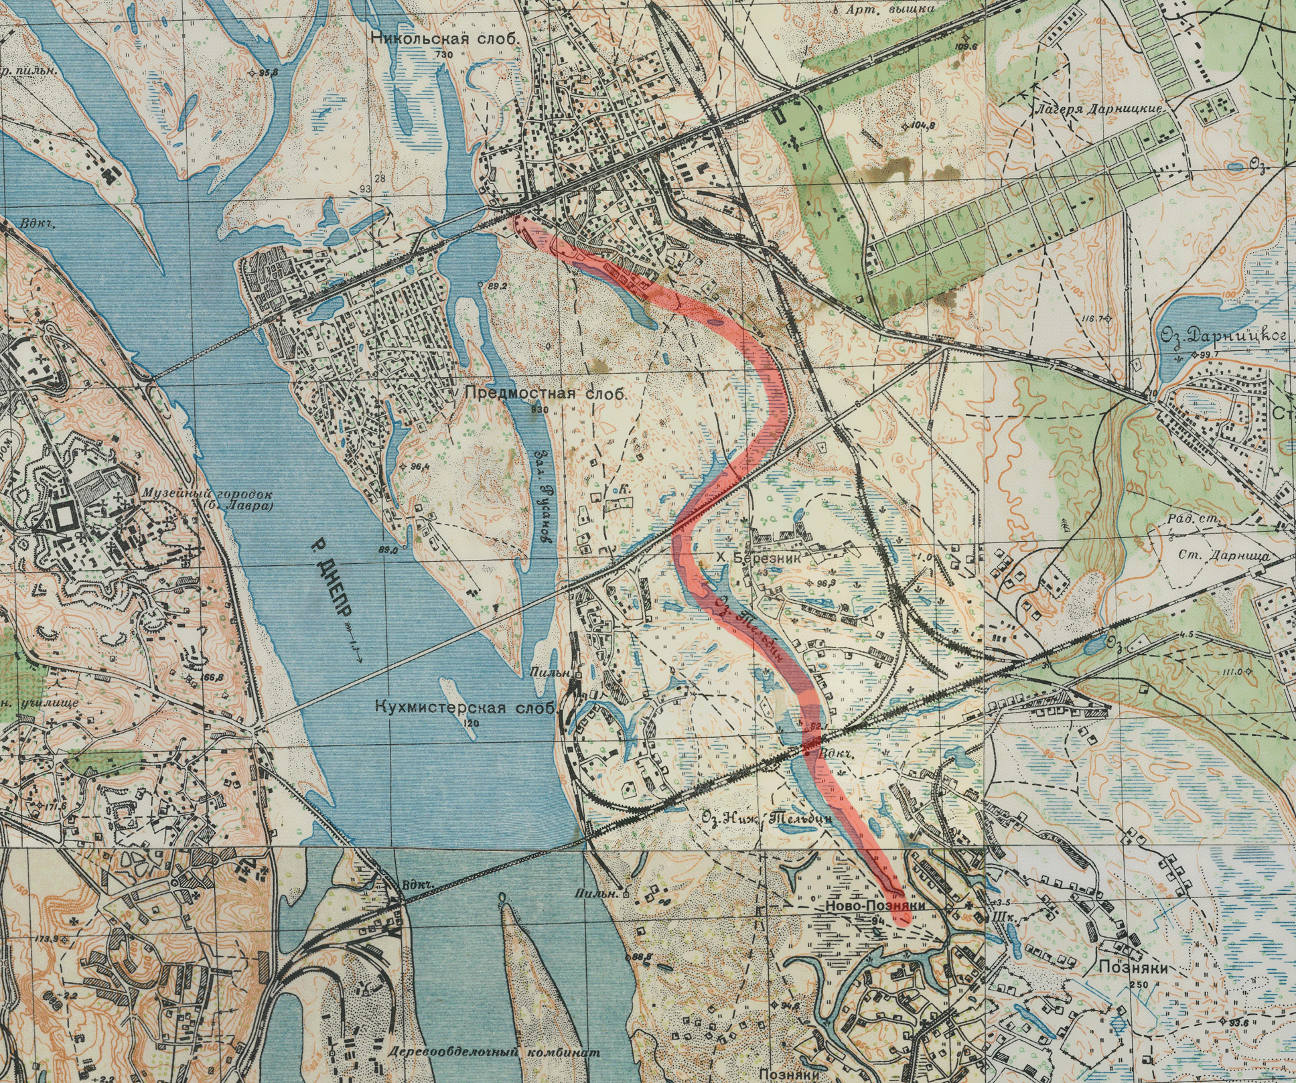
\includegraphics[width=\linewidth]{chast-gorodki/terbin/rkka-telbin-s.jpg}

\textit{На карте РККА 1930-х, красной линией я отметил остатки всего русла Тельбина-Долбина начиная от Никольской слободки.}
\end{center}

С речкой Дарницей мы будем разбираться позже, с ней тоже много вопросов. На карте Шуберта уже середины 19 века устье Дарницы – а речь идет об отрезке Дарницы, что вытекал из одноименного озера – теряется в безмерном болоте около хутора Позняки, примерно в окрестностях современного озера Горячки.

Постепенно русло Тельбина дробилось – его перерубали разные гати для прокладывания по ним дорог, а также влияли естественные причины.

Во второй половине 19 века всё к востоку от Тельбина заболачивается до Старой Дарницы.
Болото возникает и вокруг озера Дарницы – да и речка Дарница представляет в то время перетекающие друг в друга болота.

В 1860-х поперек Тельбина надо было проложить рельсы Киево-Курской железной дороги\footnote{С 1891 года переименованной в Киево-Воронежскую железную дорогу. Годы открытия участков: 1870 – от Киева до Днепровского моста; 1869 – от Днепровского моста до станции Бровары, и так далее. Чуть южнее взорванного 19 сентября 1941 г. Днепровского моста в 1949-м построили Дарницкий железнодорожный. От Днепровского моста осталось несколько опор.}. Для этого соорудили насыпь, и Тельбин распался на просто Тельбин и Нижний Тельбин. Речь идет о железной дороге, что теперь проложена через Дарницкий мост и шурует мимо Березняков к вокзалу «Дарница». Насыпь с железной дорогой поныне высится по левому берегу.

Между Тельбином и Днепром оказалось зажатой Кухмистерская слобода, что занимала нынешний квартал, ограниченный улицами Тычины, Шумского, Березняковской и Днепровской набережной. Со стороны озера на нее наползало болото – ведь после преграждения озера дамбой, вода стала накапливаться вдоль нее.

Положение исправилось позже, когда речку Дарницу направили в другое русло с выводом южнее железной дороги, в Нижний Тельбин. 

%А остатки прежнего русла ее, которое подходило к Тельбину в верхнем его течении, и поныне сохранились под именем болота Серой цапли\footnote{50°25′40″N, 30°37′13″E.} около железной дороги между заводом Фанерных плит с северо-востока и чудовищным массивом гаражей с запада. Там же начинается улица академика Шлихтера, и от железной дороги, что идет с востока на запад, отделяется еще одна ветка на север, вдоль Шлихтера (на ряде карт 2014 года ее успели раздробить на улицы Мартовскую и Вифлеемскую) и к Левобережной.

В начале 20 века русла обоих Тельбинов, простого и Нижнего, хоть и разделенные, еще сохраняли вид луговой реки. На картах они обозначались пока единым озером, доходящим до Позняков и сворачивающим у поселка в сторону Днепра. 

Но уже к 1914 году Нижний Тельбин укоротился около северной границы Позняков и на карте того года подписан «оз. Коростышево», либо такое название относится к соседнему с запада водоему. 

К востоку же от этого вытянутого с севера на юг Нижнего Тельбина было озеро Ольхово (любопытно, где ставить ударение?). Вероятно следы его – водоем близ перекрестка Ивана Кочерги и Григоренко. А остаток прежнего Нижнего Тельбина – озеро Королек между улицами Канальной и Здолбуновской, около завода высокоточной аппаратуры «Буревестник», основанного в 1967 году и работавшего тогда на оборонку.

Современный Нижний Тельбин – образование искусственное, просто широкий канал, на месте которого еще в середине 20 века был бугристый пустырь.

Посмотрим на аэрофотоснимок 1943 года:

\begin{center}
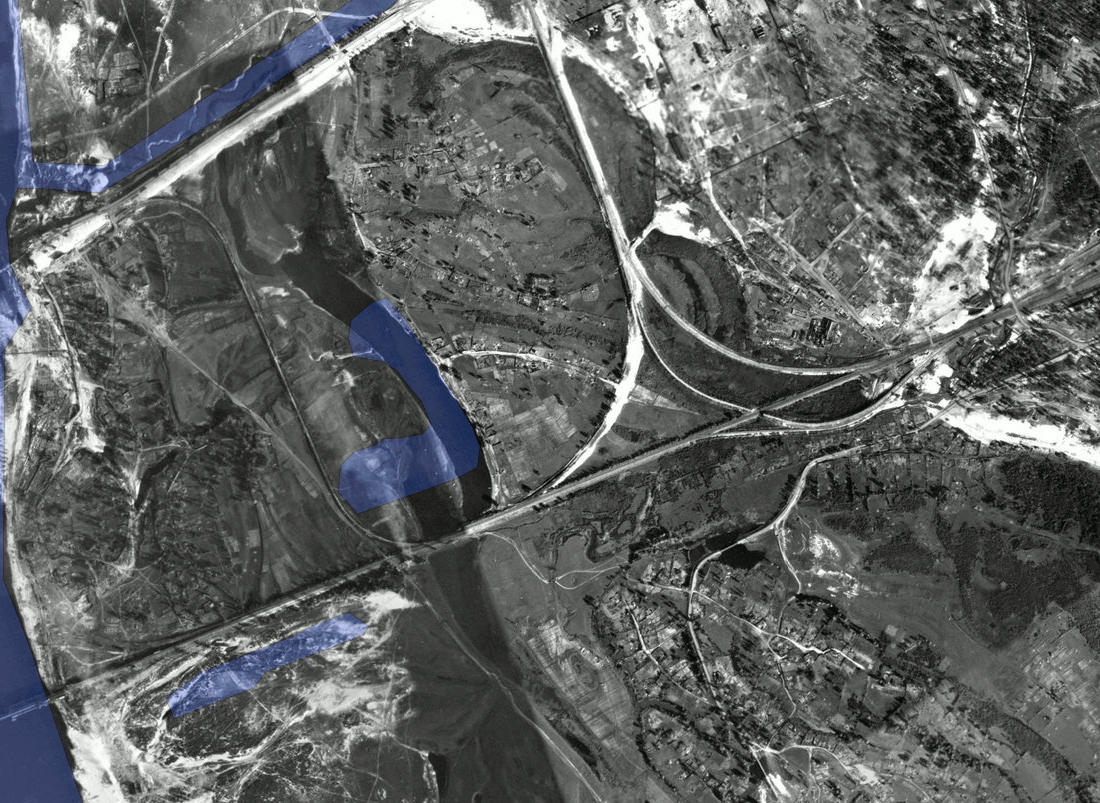
\includegraphics[width=\linewidth]{chast-gorodki/terbin/s_telbin-1943.jpg}
\end{center}

Синим цветом я отметил современный рельеф. Слева – Днепр, в верхней левой части наискось – Русановский канал вдоль современного проспекта Воссоединения. Большое синее пятно загогулиной – озеро Тельбин, синяя горизонтальная сопля – Нижний Тельбин. И сопоставьте с Тельбином за 1943 год!

Вот он начинается на севере, у нынешнего моста около остановки «бульвар Давыдова», к западу от рынка. Истока не видно, на горло ему наступила насыпь с дорогой. Насыпь? Но ведь теперь ее нет! Верно. Ведь близлежащие районы – Березняки, Русановку – насып\'али, поднимали их уровень перед строительством жилмассивов. Прежде местность была ниже, а дорога, где сейчас проспект Воссоединения, проходила насыпью по болоту. И к северу от нее застрял исток Тельбина, мы видим его – вьется змейкой вдоль насыпи, выше ее, и в сторону Днепра.

Южнее насыпи Тельбин шел по теперешним дворам в квартале между улицами Серафимовича, Бучмы, Тычины. Дом по Бучмы, 8 – стоял на озере. Детский сад №577 – на озере. Тычины 9Б – на самом берегу. Школа №191 – прямо на озере.

Современное состояние Тельбина и Нижнего Тельбина.

В Нижний отведена речка Дарница и мутный, прорытый во второй половине 20 века поток, что выходит из земли около улицы Здолбуновской\footnote{Возле 50°25'10.76"N 30°37'41.46"E.}, и протекает мимо озера Прорвы, отделенный полоской суши. На берегах его виднеются развалины частных усадеб и впавшие в дикость сады по улице Любарской (перерубленной пополам проспектом Григоренко), где на 2014 год осталось немного позняковской старины. Можете посмотреть кадры оттуда в моем фильме «Озёра Прорва и Горячка».

Затем мутный поток уходит в коллектор у проспекта Григоренко\footnote{50°25'16.87"N 30°37'17.82"E}, где соединяется с речкой Дарницей, и общие воды выходят из коллектора в канал чуть севернее начала улицы Канальной, у перекрестка с Дарницким шоссе и проспектом Григоренко\footnote{50°25'26.1"N 30°37'5"E}. Прямой канал, прорытый в 1950-х, идет на запад и ныряет в трубы под мостом Сортировочной улицы, а потом на запад от нее вливается в водоем, слывущий ныне Нижним Тельбином.

На плане 1991 года видна несколько иная картина. Тонкая синяя линия от Тепловозной улицы до впадения в Нижний Тельбин под станцией «Левый берег» – это рукотворное, но поверхностное русло Дарницы. Там, где она впадает в озеро, теперь перекресток Дарницкого шоссе и проспекта Григоренко.

Шоссе еще не существовало, его проложили в 2011-12 годах при постройке «моста Кирпы»\footnote{Автомобильный мост, построен рядом с Дарницким железнодорожным, официально оба моста называют как один – Дарницкий.}, а до этого просто шла железная дорога безо всякого параллельного шоссе. На месте массивной станции «Левый берег», почти вокзала, была обычная полустаночная платформа. %Неподалеку, в восьмидесятых, вдоль Нижнего Тельбина на пустыре была дрессировочная площадка для собак.

В 1991-м Нижний Тельбин имел вид эдакой буквы «Г» с верхней палочкой в обратную сторону. Эта палочка и есть канал. А вертикальная палочка – старое, историческое русло. Вот его-то и не стало! Теперь оно застроено серой промзоной, лишь озеро Королек, тщательно загороженное от людей бетонными заборами, напоминает, куда дотекал Тельбин – но об этом никто не знает. 

\begin{center}
\includegraphics[width=\linewidth]{chast-gorodki/terbin/1991-telbin.jpg}

\textit{Фрагмент карты 1991 года.}
\end{center}

%На берегу Королька – завод высокоточной аппаратуры «Буревестник», основанный в 1967 году и работавший тогда на оборонку. На нем производились радиоэлектронные системы наблюдения для нужд флота. 

%В первом десятилетии 21 века «Буревестник» выпускал, кроме приборов того же рода, аппараты искуственной вентиляции легких, машинки для счета купюр, FM-приемники и другие товары. 

В ходе работ над мостом и прилегающим Дарницким шоссе, на протяжении от Фанерной улицы\footnote{На этой улице был поселок рабочих Фанерного завода. Посёлок сожгли немцы во время Великой Отечественной войны. Потом Фанерка отстроилась промзоной и жилыми домами.} речку Дарницу, где она выходит из коллектора, снова туда загнали, упаковали в бетонный короб – под асфальтом Дарницкого шоссе и до проспекта Григоренко!

Про канал. Еще до того, как появилось Дарницкое шоссе, улицу Сортировочную продлили, положив поперек канала мост к станции «Левый берег». Канал условно разделился надвое – условно потому, что вода под мостом таки протекает. 

Одна часть канала, узкая – открытое прямое русло между проспектом Григоренко и Сортировочной улицей. Другая, толстая – «озеро Нижний Тельбин» между Сортировочной и Причальной. В конце 1950-х собирались строить второй речной порт, и Причальная должна была служить подъездом к нему. Но порт так и не построили.

Современный Нижний Тельбин – это западная, расширенная часть канала, продолжение более узкой части канала, а он питается Дарницей и мутным потоком со стороны озера Прорвы.
 
Ну а просто Тельбин, который верхний – его в 1970-е обсадили многоквартирными панельными домами с одной стороны, а потом уже при капитализме – небоскребами с другой. Есть пляж и довольно высокие насыпные берега. Вместо юго-западной загогулины\footnote{50°25'29"N 30°36'27"E} озера раньше было кладбище Кухмистерской слободки.

Глубина озера доходит до 7-17 метров, довольно прилично. Верхний Тельбин углубился и разросся вширь потому, что из него брали песок для намыва окрестных лугов. До того Тельбин выглядел как заболоченное озеро, с густыми ресницами камыша по берегам. Русло стали разрывать и расчищать – в то время глубина достигала даже 20 метров, и котлован наполнился чистой водой, а вокруг были горы песка да строительные краны.

Еще в 1950-х, у восточного берега озера находился хутор Березник.

Он лежал, по современным меркам, в квартале между улицами Серафимовича, Тычины и Березняковской, а также в окрестностях школы №195. Среди болот – три улицы с усадьбами, да некое посевное поле ближе к железной дороге на юге. В 1883 году хутор Зательбин Березняк имел всего 5 дворов.

Хуторское кладбище находилось, где на 2023 год пустырь у дорожной развязки при перекрестке проспекта Воссоединения с железной дорогой и улице Шлихтера, к югу от подъема проспекта на мост\footnote{50°26'15"N 30°36'42"E}. Еще не зная, что было тут прежде, я, проезжая мимо на велике, часто останавливался на этом пустыре чтобы передохнуть в тени невысоких деревьев. Хорошее место. Островок спокойствия, окруженный трассами, полными машин.

Начало пустыря занято АЗС. В конце 1960-х, время молодости жилмассива Березняки, там было футбольное поле – ну, двое ворот. 

%\begin{center}
%\includegraphics[width=\linewidth]{chast-gorodki/terbin/voss.jpg}

%\textit{Вид на проспект Воссоединения на юго-запад, от возвышения у моста, что над железной дорогой.}
%\end{center}

%До строительства Березняков, дорога, ставшая основой проспекта Воссоединения, шла по насыпи посреди болота, возникшего от Тельбина. На снимке 1964 года, когда уже существовал проспект, однако не Березняки, это болото хорошо заметно по обеим сторонам шоссе. Справа позже будет Русановский канал, слева теперь известный пустырь и пока еще зеленая зона между проспектом и жилым районом.

%Кладбище сгинуло не под подушкой песка, который намывали перед строительством жилмассива, чтобы поднять его уровень во избежание затопления при наводнениях.

До преображения местности жилмассивом, кладбище было почти на границе песчаной возвышенности, на восток от которой лежало болото. Эта возвышенность, несмотря на гидронамыв Березняков, прослеживается поныне – от перекрестка и дальше по улице Серафимовича есть длинный спуск. На месте кладбища гидронамыв не проводился, там достаточно высоко по естественным причинам. Однако бульдозеры сравняли могилы с землей.

%Кладбище не мешало и застройке, раз уж по сей день там пусто. Куда же оно подевалось? Забыто потомками или сровнено с землей бульдозерами? Последнее.

%Еще один снимок 1964 года, вид в обратную сторону, от перекрестка у моста Патона в начале проспекта Воссоединения. Справа через несколько лет начнут расти девятиэтажки Березняков.

%\begin{center}
%\includegraphics[width=\linewidth]{chast-gorodki/terbin/1964aug.jpg}
%\end{center}

Но где было устье Тельбина? Я не знаю точно, но южнее Позняков.

Теперь про Золочу. В летописи ошибка. Правильно не «Золоча», а «Волоча». Мы ведь знаем, что Гюрги волочил лодьи из Долобского в «Золочу». К счастью, около Бортничей еще в 19 веке сохранялась память о речке Уволочье\footnote{Недалеко от Витачова и другого брода, Зарубского, у горы Зарубы.}! Сейчас картографы с подачи ученых усердно переименовали её в «озеро Золоче», но это натяжка. Далее я буду везде писать Волоча. Ввожу такое название в обиход, точнее, возвращаю его.

Принято считать, что Волоча протекала от Киева, примерно от Березняков и на юг мимо Позняков, Осокорков, Бортничей, Гнедина и Вишенок. Но от Березняков до Позняков и несколько южнее был Толбин. Значит, Волоча начиналась еще ниже.

Если взять современную карту, то мы увидим – да, вот «оз. Золоче» чуть южнее Гнедина (Гнедыни), а вот рядом с ним Прорва (не позняковская, а другая Прорва), в районе же Бортничей в связи со станцией аэрации и ее канализационными лугами водная система сильно искажена. Как было прежде?

Карты Шуберта в помощь! Без Бортнической станции аэрации! Фрагмент листа 9, ряда XXII:
\vspace*{\fill}
\begin{center}
\includegraphics[width=\linewidth]{chast-gorodki/terbin/s_volocha-01.jpg}
\end{center}
\vspace*{\fill}
\newpage

Что же мы видим? У Позняков и Осокорков сам черт голову сломит. Выверты низовий Тельбина, какие-то громадные старицы у болота урочища Небреж. А вот от Бортничей начинается будто цельная река. Оттуда на юг мимо Гнедина, Вишенок.

Поглядим на лист карты Шуберта, который лежит южнее. Это лист 9, ряд XXIII. Здесь продолжается река, идущая от Бортничей вдоль Гнедина и Вишенок. В верхней правой четверти, параллельно Днепру, видно ее устье. Какая стоит подпись? «Р. Уволочье». Речка Уволочье!

\begin{center}
\includegraphics[width=\linewidth]{chast-gorodki/terbin/s_volocha-02.jpg}
\end{center}

Очевидно, что это – сохраненное именно старожилами название, и полагаю, что летописная «Золоча» впадала в Днепр именно здесь. Только букву «З» считаю ошибочной, ибо название Волоча оправдано волочением туда судов и прижилось в обиходе вплоть до 19 столетия, превратившись в Уволочье.

Низовье этого «Уволочья» современные уже картографы переделали в «озеро Золоче», наверное полагая, что восстанавливают историческую справедливость. Так или иначе, Волочу еще можно проследить на карте 21 века от Бортничей и на юг. Судя по имени одного из озер около Бортничей – Млынного – на этой части Волочи стояла водная мельница.

Мне остается в этой главе попробовать объяснить название Долобского и его производного – Тельбина.

В летописи есть рассказ о народе Дулебов:

\begin{quotation}
си бо Угри почаша быти при Ираклии цари, иже ходиша на Хоздроя царя Перьскаго.

В си же времена бысть и Обре, иже воеваша на царя Ираклия и мало его не яша; си же Обри воеваша на Словены и примучиша Дулебы, сущая Словены, и насилье творях женам Дулебским: аще поехати бяше Обрину, не дадяше въпрячи коня, ни волу, но веляше въпрячи 3, или 4, или 5 жен в телегу и повести Обрина; и тако мучаху Дулебы.

Бе бо Обри телом велици, а умом горди, и потреби я Бог, и помроша вси, и не оста ни един Обрин; и есть притча в Руси и до сего дни: погибоша аки Обри; их же несть ни племени, ни наследка.
\end{quotation} 

Возможно, летописное озеро «Дулебское», ставшее потом Долобским, как-то связано с этими Дулебами.

\chapter{Речка Дарница}

Я много упоминал речку Дарницу, так что придется рассказать о ней подробнее. Дарнице посвящена отдельная серия «Киевской амплитуды», но когда мы снимали ее, то не видели еще старинной польской карты\footnote{Эту карту 1640 года я по сей день хорошо не рассмотрел. У меня есть кусок в хорошем качестве, и полный скан в качестве отвратительном.}, где четко обозначена эта река, и предполагали исток около Княжичей, в Ялынке, а на деле его следует искать в Броварах или к северо-востоку от них. А может, того истока уже нет и он сместился к Ялынке.

Вообще имя Дарницы носила и местность (причем одноименная станция метро не имеет к ней  отношения), и огромное озеро, и речка – эта глава посвящена больше именно последней.

Помню, снимали мы про Дарницу долго, много разрозненных съемочных дней, почти всё лето 2013 года, самого плодовитого на серии. Пешие походы по жаре, и в тени через комариный рай, и лесом на велосипеде.

Река Дарница раскинулась по всему Левому берегу и нельзя за один присест ее обойти. Ни над одной рекой так не издевались – и отходами загаживали, и на части разделяли, а сейчас кое-кто вовсе отказывает ей в историческом существовании – мол, нет такой речки, есть Северодарницкий мелиоративный канал.

А ведь прежде всё было иначе. Жила-была речка Дарница. Вот она на той самой польской карте:

\begin{center}
\includegraphics[width=\linewidth]{chast-gorodki/darn/s_1992-kroynika.jpg}
\end{center}

Дарница подписана здесь как «Dranica». В верхней левой части два населенных пункта – Бровары и Княжичи. Дарница протекает мимо них, в виде двух наверное прудов, очень раздутая, почти как Днепр. Ничего удивительного в этом нет, подобные пруды по сей день находятся на речке Борщовке.

В Броварах есть несколько разрозненных озер, и одно из наибольших – в парке Победы. Юго-восточная часть парка стоит на костях, там было еврейское кладбище, и поваленные надгробия встречались еще в начале двухтысячных. Если залезть в парке на курган и смотреть в сторону, противоположную от озера, на рощу – там и было кладбище. Я плохо знаком с прошлым Броваров, поэтому не знаю, что это за озеро. В конце 1980-х в парке был наполненный водой бетонный канал, вдоль улицы Воссоединения, со стороны улицы Гагарина. Словом, броварской след в происхождении Дарницы для меня неясен.

Изображенная на польской карте толстая часть Дарницы от Броваров до Княжичей, на трехверстовках Шуберта середины 19 века превратилась уже в подобное луговой реке «озеро Свидловщину», к востоку от коего распространилось болото. Свидловщина близ северо-западной границы Княжичей поворачивало на запад к железной дороге да озеру Рыбному. Сейчас на отрезке от Броваров до Княжичей – район Княжичей Ялынка, прежде бывшая дачным поселком. Там есть одноименная железнодорожная станция. Дома между нею и Княжичами называют Ялынкой, но по адресам улицы последней относятся ко Княжичам.

\begin{center}
\includegraphics[width=\linewidth]{chast-gorodki/darn/s_1850-darn.jpg}
\end{center}

Дарница в образе Свидловщины огибает Ялынку по восточной, затем по северной границе эдак до 7-й Садовой улицы. Вода почти всюду покрыта зеленой ряской.

Ялынка весьма точно вписывается между Свидловщиной и железной дорогой. Далее вода Дарницы течет ручьем южнее озера Рыбного, образуя по пути каскад озер и болотец. Какую роль озеро Рыбное играет в этой водной системе, не знаю. Затихшее, огромное – полкилометра на четыреста метров, пусто раскинулось в лесной плеши лесом рядом с «быковнянскими могилами» (они кстати гораздо ближе к хутору Рыбному, чем к Быковне) и заброшенными строениями свинофермы. Издалека видно тамошнюю водонапорную башню.

В 2013 году я, вооружившись видеокамерой и фотыком, на велосипеде отправился исследовать участок Дарницы в том краю. Повернув на север от Броварского шоссе, безлюдной дорогой через лес поехал к хутору Рыбному. Улица, несколько домиков, рядом припаркованы машины. Несколько местных во дворах. Играющие дети. Колесить по хутору мне не хотелось, в памяти возникли шаблонные американские фильмы ужасов, где одинокий путник, сбившись с пути, попадает в захолустный городок, жители коего настороженно смотрят из окон. Неподалеку, я знал по карте, расположена скотобойня. Поддал крутить педали.

Дорогу к Рыбному озеру я тогда не нашел. В лесу разбегалось много бугристых дорог, все грунтовые, точнее из плотно сбитого песку, и даже мой огромный дорожник «Аист» отчаянно буксовал. GPS, как обычно, не хотел запускаться, поэтому на перекрестках я руководствовался наитием. Наитие привело меня к болоту, откуда я услыхал шум проходящих поездов и понял, что если буду следовать на него, не пропаду. Я залез на сухое дерево над болотом, поснимал водную гладь, затем вжарил скорость, обогнав двух туристов. Сбоку возник песчаный косогор. На верху росли сосны.

Где-то здесь, в окрестностях Ялынки, в восьмидесятых годах мы с отцом катались на великах. Я был мал, и велосипед мой был мал – складной «Минск» (потом его называли «Аистом»). Тогда мы попали под ливень и размокшими дорогами пробивались назад к электричке.

А сейчас я понял, что заблудился. Поезда перестали свистеть. Впереди шла женщина лет сорока-пяти, с корзиной, в спортивных штанах и вязаной кофте на голое тело. Небось собирала в лесу разное зелье. Я спросил, как проехать к железной дороге, женщина стала обстоятельно рассказывать, как удобнее, особенно на велосипеде, но я ничего не понял, поблагодарил и стал вкручивать педали дальше.

Хвойный лес сменился лиственным. Я достигнул гати через Дарницу, что текла под насыпью через несколько ржавых труб. По обе стороны дороги было довольно приличное русло, а вот водичка едва покрывала дно, растекаясь по ширине. Около труб прыгали маленькие коричневые лягушки.

Я последовал вдоль русла, сколько мог с велосипедом, а затем выбрался таки к железной дороге (как понимаю теперь, в урочище Мостище, чье имя указывает на давний мост), но до самой Ялынки не поехал, отложив на потом. Вместо этого покатил рядом с рельсами весьма неудобной тропкой.

Вся эта местность называлась Плеховским болотом. Вот во что превратились пруды, на которых стояли водяные мельницы. В наше время болото несколько усохло и от железной дороги отдалилось. Сквозь жутковатую чащу я его не видел. Долго ли, коротко, свернул наобум вправо. Там и нашел остатки прудов. Места эти своей безлюдностью и вместе с тем ощущением чьего-то присутствия, некоего ожидания, напоминают мне фильм «Пикник у Висячей скалы».

От Ялынки руслу Дарницы придан вид ломаной линии – она давно уже не петляет обычной полевой рекой, но сочится по спрямленным участкам русла, наполняя пруды.

Из пруда в пруд вода с шумом перетекает через трубы:

\begin{center}
\includegraphics[width=0.51\linewidth]{chast-gorodki/darn/s_darn-IMG_2747.JPG}
\end{center}

\newpage
\vspace*{\fill}
\begin{center}
\includegraphics[width=\linewidth]{chast-gorodki/darn/s_darn-IMG_2743.JPG}
\end{center}

\begin{center}
\includegraphics[width=\linewidth]{chast-gorodki/darn/s_darn-IMG-2745.JPG}
\end{center}
\vspace*{\fill}
\newpage
\vspace*{\fill}
\begin{center}
\includegraphics[width=\linewidth]{chast-gorodki/darn/s_darn-IMG_2756.JPG}
\end{center}

\begin{center}
\includegraphics[width=\linewidth]{chast-gorodki/darn/s_darn-IMG_2751.JPG}
\end{center}
\vspace*{\fill}
\newpage

Вот так и прежде – были пруды, а при них заводились мельницы, что способствовало обмелению Дарницы и заболачиванию прилегающих земель. Документально мельницы известны на Дарнице еще с начала 16 века. 

В решении межевого суда о границах владений Печерского и Николо-Пустынного монастырей на земле Зверинской, 1508 года сказано\cite[том 4, часть 8, стр. 160]{akty02}:

\begin{quotation} 
реку Дарницу, на которой же реце и млынища, што перед тым стого\footnote{Стого – святого.} Николы Пустынского млын был, и на тои гребле есмо стояли [...] тое дей млынищо и с тым озером гдрское\footnote{Господарское.} нам жалование
\end{quotation} 

Млынище (место прежней мельницы) на речке Дарнице упомянуто и в грамоте 1516 года. Проходит 200 лет, а реку всё используют, чтобы крутить колеса мельниц. В жалованной грамоте в Киевопечерскую Лавру на владения Троицкому Больницкому монастырю, 1720 года, записана «мельница Дарницкая нижняя»\footnote{Возможно, она стояла к юго-востоку от нынешней Дарницкой ТЭЦ – возле нее было озеро Дарница, после коего речка продолжала свой ход, и там-то на карте 1799 года показаны два пруда, а значит могли быть и мельницы.}. Где-то при Дарнице и Княжичах, в 18 веке были и хутора, объединенные именем «Дарницкого».

Между Быковней и ДВРЗ\footnote{Дарницкий Вагоно-Ремонтный Завод, завод и посёлок на окраине Киева. От зданий на главной улице веет сталинской архитектурой.} есть место, где еще в первой половине 20 века квакало Плеховское болото, а теперь рябит волнами большое озеро Березка (Берёзка есть и в Гидропарке), оно же Лесное. Это в 1954-м работники Дарницкого Вагоноремонтного завода расчистили участок болота. В том же году, маршал Будённый торжественно открыл в ДВРЗ местный дом культуры, выстроенный по проекту архитектора Соколовского.

Озеро красивое, в восточной части даже обустроенное – есть лодочная станция. На выходных берега заняты приезжими. Автомобили, шашлычный дым, привет природе! А ведь в Березке и около водятся остромордая лягушка, тритоны, богомолы, болотные черепахи, раки, водяные крысы, выдры, бобры!

\begin{center}
\includegraphics[width=0.93\linewidth]{chast-gorodki/darn/s_darn-IMG_20130720_144259.jpg}
\end{center}

На Березку, привлеченные клочками песчаного пляжа, ездят отдыхать из Быковни и ДВРЗ, да и со всего Киева. Обочины окрестных лесных дорог служат свалкой для разного строительного мусора. На одной из таких я нашел множество разбитых табличек с кладбища домашних животных. Озеро окружено соснами да березами. Березняк стоит на темной, торфяной почве и здорово обжит комарами, сосны же вгрузли корнями в солнечный песок. Со дна Березки тянутся водоросли, в которых запутываются купальщики. Вода часто цветет густой зеленью, будто туда вбухнули тонну акварели. Ручей, а собственно Дарница, от Плеховских болот присоединяется к озеру в восточной его части, посредством бетонного желоба.

Дарница за Ялынкой вошла в систему мелиоративных каналов в 1930-х. Уже тогда речное русло начали спрямлять, заключать в укрепленные берега, и отводить в водосборы других рек.

\newpage

Из озера Берёзки Дарница вытекает по двум совершенно разным руслам.

Примерно из северной точки (немного восточнее) Березки выходит канал, что очень скоро раздваивается. Одно русло идет прямо через лес на запад к улицам Попудренко и Мурманской. К этому руслу легко выбраться, свернув в лес напротив супермаркета «Новус» на Попудренко. Оно захламлено шинами и порой пересыхает – зависит от уровня воды в Березке.

\begin{center}
\includegraphics[width=\linewidth]{chast-gorodki/darn/s_darn-IMG_20130720_141133.jpg}

\textit{Снимок 2013 года.}
\end{center}

Сие русло тоже разветвляется. Один канал питает озеро за типографией «Блиц-принт» (что к востоку от станции метро «Лесная»), другой сворачивает резко на юг вдоль этой типографии, к заводу химикатов «Радикал», проходит между ним и лесом, и затем на юг же, мимо железнодорожной станции «Лиски»\footnote{Станцию построили для нужд Дарницкой промзоны к северу от одноименного района, возникшего на месте болота Лиски (Лески), лежавшего по историческому руслу Дарницы. Близ болота в 20 веке возник одноименный хутор. Точно на его месте теперь частный сектор между улицами Станюковича и Сновской. Местность на юго-запад оттуда, между улицами Пражской, Азербайджанской и Алма-Атинской, считалась Старой Дарницей.}, огибая ее восточную сторону. Вообще канал от Березки к «Блиц-Принту», потом через Лиски – это всё примерно по ходу старого русла Дарницы и болот вдоль него. Болота частично еще живы.

% Район же находится между станцией и Старой Дарницей, и плавно переходит в последнюю. Скажем так – Лиски это частный сектор в окрестностях улиц Калачёвской и Новаторов. Граничит с промзоной. Добраться в Лиски можно трамваем с Ленинградки на ДВРЗ. Выйти на остановке «Профсоюзная».}

На краю поселка ДВРЗ, у последних номеров улицы Олексы Довбуша, канал сворачивает на запад. Тут русло канала сохраняется неизменным с конца тридцатых годов. Оно направляется к улице академика Бутлерова, пересекает ее и заходит на территорию Дарницкой ТЭЦ. На Бутлерова Дарницу, весьма в том месте вонючую химикатами, можно пощупать около моста над нею. Русло с одной и другой стороны моста уходит под ограды. К открытой речке проще подобраться со стороны заброшенных железнодорожных путей, идущих от Киев-Лиски на север.

А следуя вдоль ТЭЦ на юго-запад, на пути к пересечению с Красногвардейской, канал прячется в коллектор\footnote{50°26'36"N 30°38'32"E}.

К юго-западу от Дарницкой ТЭЦ раньше, с 19 века и до строительства ТЭЦ в 1950-х, было большое (в 1930-х длина более 700 метров, ширина около 400) озеро Дарница, откуда река руслом (а позже новым каналом) протекала далее. Озеро, по нынешним меркам, охватывало самый северо-западный край ТЭЦ, промзону у перекрестка Павла Усенко с Красногвардейской, и до перекрестка Азербайджанской с Пражской. Вот там, за Азербайджанской номер 1, еще в 2008 году было небольшое озерцо – остаток прежнего Дарницкого! Нет уже и его. А ведь еще в начале 21 века местные жители вроде бы добились от государства решения на устройство парка вдоль русла Дарницы от Пражской и до самого Харьковского шоссе. Увы.

Вероятно, раньше Дарницкое озеро было еще больше, чем в первой половине 20 века. На карте 1799 года на нем заметны два острова. Я знаком с этой картой отрывочно и не могу соотнести размер озера с чем-либо, кроме тогдашней Кухмистерской слободы. Видимая на куске карте часть озера была эдак впятеро больше площади слободы. Тогда же, от озера речка протекала дальше на запад, примерно в сторону слободы, но забирая к югу. Вдоль западного берега озера шла дорога, по ней мост через вытекающую из озера речку, на речке – два пруда, у самого моста – «шинок Дарница», а к северу оттуда по дороге же – «трактир городской именуемый Красный».

А ныне, нырнув под Пражской, течет Дарница дальше в подземном коллекторе вдоль улицы Лохвицкой, прямо под новостройками жилищных комплексов «Родинний затишок», «Флагман», «Новая волна», «Стародарницкий». В этом месте и хотели парк вдоль речки. Подобный ход Дарницы справедлив по карте РККА 1930-х, а вот согласно Шуберту, в середине 19 века русло лежало значительно западнее. Ошибается карта Шуберта или русло переместилось?

Здесь вдоль него, на 2016 год – теснимый небоскребами и гаражными кооперативами сохраняется еще частный сектор по улицам Сосницкой, Краснокутской, Двинской и смежным с ними. Не редкость кривые заборы с калитками. Встречаются и двухэтажные многоквартирные домики.

\begin{center}
\includegraphics[width=0.85\linewidth]{chast-gorodki/darn/s_darnica-DSC_0022.JPG}

\textit{Старая Дарница 2013 год.}
\end{center}

Селиться тут стали в начале 1950-х, а до того был лес. Это место относится к Старой Дарнице. А Новая Дарница – на юг от железной дороги, станции «Дарница», где современный квартал между Харьковским шоссе, Ялтинской и Привокзальной.

\begin{center}
\includegraphics[width=\linewidth]{chast-gorodki/darn/s_darnica-DSC_0020.JPG}

\textit{Старая Дарница, 2013 год.}
\end{center}

Пройдя под Харьковским шоссе, речка Дарница выбирается на поверхность по улице Фанерной, за институтом химии\footnote{50°25'50.5"N 30°38'01.6"E}. К тому времени она стала полноводней. Приблизившись к железной дороге, речка снова уходит в коллектор, но какие-то соки продолжают питать перекроенную насыпями местность, образуя «болото Серой цапли» (часть прежнего русла Дарницы), и воспетый экологами «реликтовый Мокрый лес»\footnote{50°25'34.05"N 30°37'34.38"E} по другую от болота сторону насыпи. В 2013 году там остановился цыганский табор, и Мокрый лес превратился в огромный нужник и мусорную свалку.

\begin{center}
\includegraphics[width=\linewidth]{chast-gorodki/darn/s_darnica-DSC_0026.JPG}

\textit{Болото Серой цапли, 2013 год.}
\end{center}

Оба названия современны, кажется, в ходу с семидесятых годов.

Дарница на этом протяжении взята в коллектор и выходит оттуда западнее, у начала Канальной улицы и перекрестка с проспектом Григоренко. В коллекторе она смешивает воды с мутным потоком, идущим вдоль озера Прорвы по прорытому на рубеже нулевых каналу стока воды из озера Солнечного.

Близлежащее озеро Жандарка, окруженное уже не частным сектором, а высотками, за десятилетие до 2014 года полностью изменило форму и размеры в связи с перепланировкой местности. Частный сектор с улочками Тальновской, Внешней, Зоотехников, Батуринской исчез, там сейчас новостройки, из старых улиц сохранились только Днепровая и Ивана Бойко. К востоку от Бойко был и остается длинный водоем с заводями (его видно с юго-западной стороны перекрестка Здолбуновской и Григоренка), а вот на месте современного здоровенного, позеленевшего озера Жандарки еще в конце первого десятилетия 21 века протекал ручей. Отмотав время еще на 20 лет назад, к 1990-м, мы обнаружим вместо «длинного водоема» ручей с цепью прудов на нем. Как всё изменилось!

Я не зря об этом пишу. Ведь ручей был некогда продолжением нижнего течения Тельбина, продолжаясь до Осокорков, а как дальше – не ведаю.

Но вернемся к Дарнице.

Канал вдоль Канальной улицы следует на восток, мимо станции «Левый берег» и шумного шоссе. Зеленые бурьяны, закрывшие собой берега, скрыли горы свезенного сюда строительного мусора, где попадались старинные кирпичи. По другую сторону от шоссе, через реку, за старыми деревьями приумножаются гаражи и промзона.

Я помню это место в восьмидесятых. Лето, синее высокое небо, полустанок, а под насыпью, на пустыре – площадка для дрессировки собак, и обросшее камышом озеро Нижний Тельбин.

А в 2013 году, по левому берегу Нижнего Тельбина –  той части канала, что прокопана ближе к Днепру – тянется, между водой и улицей Канальной, пустырь, успевший у берега порасти деревьями. Чахлая трава щедро усеяна хламом. К озеру со всех сторон подбирается стройка. Строители ловят рыбу, еще какой-то мужичок ловит рыбу, неведомо кто жжет костер из резины. 

Мы заканчиваем снимать очередную ходку «Киевской Амплитуды», полчаса назад попали в бешеную пылевую бурю, когда даже деревья размахивали ветками, чтобы отогнать ветер. До транспорта идти еще порядочно, к набережной Днепра и Русановке. Я растер себе ноги берцами\footnote{Которые убились только осенью 2016 года при исследовании с Колей Арестовым склонов ботсада на Зверинце.}, зато в них удобно было шагать по камням около рельсов, где я подобрал несколько кусков кремния, заподозрив в них первобытные орудия. Тучи исчезли, засветило солнце.

От Набережной мы перешли на другую сторону улицы, и я пошел к маршрутке, а в камере осталось снятое за день видео, да в мобилке – несколько расплывчатых снимков, потому что там накрылась матрица, и фотографии получались с налетом нежной грусти.

\begin{center}
\includegraphics[width=\linewidth]{chast-gorodki/darn/s_darnica-DSC_0028.JPG}

\textit{2013. Нижний Тельбин.}
\end{center}

Вода из Нижнего Тельбина уходит в Днепр, но это не конец Дарницы, а лишь одно из устий. Ведь существует вторая ветвь канала от озера Берёзки!

Два съемочных дня ушли на его исследование, хотя в разное время я был на его отрезках и раньше, а порой бывал и позже.

Второй канал идет от Березки на северо-запад, к западной границе посёлка Быковни, где еще в середине прошлого века по обе стороны шоссе было два озера.

Канал ныряет под Броварское шоссе и обретается на коротком отрезке по улице Кузбасской, после чего в коллекторе следует на северо-запад, пересекает улицу Киото и выходит рвом в Быковнянском лесу. Там речка Дарница с переменным успехом течет в направлении Лесного массива. Вода в канале зеленая, иногда невозможно понять, стоит она или движется. В 2013 году с севера канал получал приток – ручей с примесью железистых частиц. К 2016 году этот ручей высох.

В окрестностях станции метро Лесная, в лесу, канал поворачивает вдоль улицы маршала Жукова и прячется там в коллектор, чтобы выйти наружу в противоположной части Лесного массива, за автоматической телефонной станцией на Милютенко, 29.

Это положение дел на 2016 год. В лесу поныне остались пересохшие мелиоративные каналы, наибольший из которых заканчивается у южного конца Лесного кладбища. Мы сейчас подобрались к теме, которую я широко буду развивать в главе о Радунке – про водную систему на Троещине, Воскресенке, Радужном. Так получилось, что воды Дарницы и мелиоративные каналы искусственно вмешались в жизнь этой местности, и моя задача – попытаться размежевать исконные речки и канал Дарницы.

От Милютенко канал шпарит на северо-запад по местности болота Казенного, к 21 веку весьма пересохшего, но кое-где сохранившегося. В середине 20 века тут было большое озеро, окруженное болотом. Оно питалось от ручья, что начинался чуть северо-западнее перекрестка улицы Жукова и Лесного проспекта. Ручей ныне смешивается с речкой Дарницей и составляет б\'ольшую часть объема воды в канале, если не всю, ведь в последние годы уже на приближении к Лесному, мелиоканал от речки Дарницы почти высох. Поэтому именование канала Дарницей дальше, за Лесным, весьма условно.

На участке леса между улицами космонавта Волкова, Братиславской и Крайней, среди березняка – водянистые, буйно заросшие торфы с кочками да ручейки. По этому-то Казенному и течет в канале вода.

Сначала, по выходу из коллектора у телефонной станции, она страшная – черная. Набросано много автомобильных шин и прочего хлама. Стоит гнилая вонь. Надо думать, черный цвет – это размытый болотный торф. Поперек леса, с востока на запад до Куликово – старая грунтовка с деревянными столбами\footnote{От 50°29'1.17"N 30°37'25.18"E до 50°28'47.33"N 30°36'36.54"E, и далее на север. У канала и под Братиславской дорога прерывается.}. 

Еще более старая дорога, кажется многовековая, находится в лесу между улицей космонавта Волкова и Лесным кладбищем, прерванная ныне последним, и сворачивает потом на восток по высокому берегу Алмазного озера, бывшего болота, и дальше в направлении Броваров. Шлях этот виден даже на плане Шуберта, однако уцелел по наше время не полностью.

Но вернемся к каналу. Ближе к улице Крайней слышны голоса людей, люди там заняли участок леса и всячески назойливо отдыхают. За полторы сотни метров от перекрестка Братиславской с Крайней, Дарница уходит в коллектор под Воскресенкой. Диггеры плавали по нему в надувной лодке.

Местность вдоль южной части Крайней и оттуда к Петра Запорожца и Курнатовского была прежде занята болотом Куликово. Лес на восток от Братиславской и сейчас, посуху, перекроен каналами да гатями. А Куликовым теперь называется район в треугольнике Братиславской – Курнатовского – Стальского, застроенный в 1980-1982 годах девятиэтажками. Во второй половине прошлого века Куликовым считалось еще и место, где нынче Троещинский вещевой рынок. Прежде болото северной развилкой достигало его южной и восточной границ.

В первой половине 20 века болото Куликово составлялось из двух рукавов. Один, частично сохранившийся, лежит вдоль улицы Крайней. Другой начинался у теперешнего дома по адресу Братиславская, 18Б и шел между шоссейной часть улицы и домами, где сейчас полоса поросшего деревьями и травой пустыря. 

На юго-запад от перекрестка Крайней и Братиславской (где оба русла смыкались), примыкая к району Куликово, есть метров двух глубиной ложбина вдоль леса, оставшаяся от общего болотного русла. В ней, ее приближенной к перекрестку части, изредка появляется вода и имеет течение на юг. Всё носит следы облагораживания – кажется, в советские времена тут был оборудован даже пляжик (остались бетонные ступени). Сохранились остатки неких хозяйственных сооружений – перегородки с дверцами.

В конце тридцатых или самом начале сороковых годах двадцатого века там проходил мелиоративный канал, до места, где сейчас роддом около перекрестка Курнатовского и Петра Запорожца. Туда же в конце тридцатых проложил новый (взамен прежнего) канал от проточного озера на юге отсюда.

Это возле станции метро «Дарница» есть парк Победы\footnote{В середине 1980-х мы пару раз ездили в гости к знакомым, что жили в огромном полукруглом доме около этого парка, через улицу. Выбрались погулять и в парк, где стоит семиметровый курган Бессмертия (первое и полное название «Курган Бессмертия в память о тех, кто отдал свою жизнь за власть Советов»), торжественно открытый, как и парк, в 1967-м. Он насыпан из земли с солдатских и партизанских могил. Основание кургана – в виде пятиконечной звезды, хотя сам выглядит пирамидой. Так вот, знакомые рассказали, что по ночам над курганом наблюдают странное свечение.}. До парка, здесь загнивал заболоченный ручей с несколькими озерцами по нему, хотя еще в 1930-х там было большое заболоченное озеро\footnote{На карте РККА 1930-х на западном берегу обозначен некий «Питомник».}, занимавшее пространство от современной улицы генерала Жмаченко до жилого комплекса «Парковые озера». Русло этого озера, как хорошо прослеживается на старых картах, да и на местности – продолжение того же древнего водоема, часть которого заняло болото Куликово.

В 2004 году ручей превратили, в пределах парка в – ну как сказать – полевую реку длиной один километр. Небольшое течение, вода понемногу выходит через трубу из северной части водоема, движется под проспектом Алишера Навои и ровным наземным каналом дальше на север, через лес, вдоль Курнатовского, к больнице и роддому. Не доходя до него, уходит в коллектор. И в нем уж соединяется с водами Дарницы.

Вторгнувшись по Воскресенскому коллектору в чужой водосбор, водосбор Радунки, Дарница под землей идет севернее Радужного озера, на запад, минует очистные сооружения на улице Петра Вершигоры, проходит под противопаводковой дамбой и вскоре, за озерцом у пустыря, впадает в залив Десёнку.

%Вот я и закончил рассказ о Черторые, Тельбине и Дарнице. О последней просто к слову получилось, да и всё равно пришлось бы потом объяснять, откуда взялась дополнительная вода там, где ее раньше не было. Мог и короче, без слободок, да про них знают мало, как не поведать? Хорошо хоть о мото-трамвае развить мне помешали иллюстрации, а то бы еще добавил, что линию его в конце двадцатых таки электрифицировали, и по мосту Бош перед войной ходил уже лектрический трамвай, а не переделанные на рельсовый ход грузовики.

%Набравшись сил, продолжу свою повесть о левобережных реках, подбираясь к Городку, хотя не он здесь самое любопытное.

\chapter{Сёла Выгуровщина и Троещина}

Вскоре мы плотно займемся странным земляным сооружением – погребальным валом, отождествленным учеными с... остатками замка  князя Симеона Олельковича, а впридачу с летописным Городком. С этим я поспорю много дальше, тут бы сначала прояснить вопрос – а где было это, как говорит наука, «городище»?

Источники сообщают про известный в узком кругу вал на берегу озера Гнилуши. Поскольку оно неразрывно связана с селами Выгуровщиной и Троещиной, я расскажу сначала о них, и потом только двинемся дальше.

Современный жилмассив Вигуровщина-Троещина поглотил б\'ольшую часть села Выгуровщины, и лежит на восток от уцелевшего села Троещины. Мне придется постоянно уточнять, когда говорю о жилмассиве, а когда о селе. От села Выгуровщины по 2016 год осталась юго-западная часть.

Жили-были почти рядом два села. Троещина с некоторых времен до 1877 года, когда случилось большое наводнение, лежала севернее Выгуровщины, на берегу русла, что именуют теперь Десенкой. Потом Троещина переехала восточнее. По Выгуровщине серпом проходил также пруд, на карте лоций 1914 года подписанный как «оз. Ставок (б. пр.)», на карте Сноевского – «река Прудок», на карте 1719 года – «речка Пруд». 

Троещина названа потому, что это было владение Больницкого Троицкого Монастыря Киево-Печерской Лавры. Само село Троетчина известно с 18 века. Было к северу от нее и Троецкое озеро. А Выгуровщиной владел Ян Выгура, вроде бы завещавший село Михайловскому Златоверхому монастырю. Прежде на месте Выгуровщины находилось летописное селение Милославское. Кстати, была еще Милославщина у Витичевского брода, много южнее Киева.

С течением лет граница между Троещиной и Выгуровщиной менялась. По числу дворов Выгуровщина всегда преобладала. В 1766 году в Троещине было 28 дворов и 256 человек населения, а Выгуровщина в то же время насчитывала 42 двора с 409 душами. По состоянию на 1917 год, Троещина – 260 дворов, 1531 житель. Выгуровщина – 391 двор, 2210 душ. На 1939 год, Троещина – 436 дворов, 2099 жителей. Выгуровщина – 609 дворов, 2607 жителей.

К половине двадцатого века обжитые земли сёл соединились, однако формально объединение произошло в 1957 году – оба села записали в Троещину. Жители продолжали их различать, хотя не всегда правильно.

Различали еще и Оболонье, между Воскресенской слободкой и Выгуровщиной. Оболонье лежало у нынешнего перекрестка Ватутина и Бальзака, эдак от улицы Петра Вершигоры и включая первые номера домов на Бальзака. Официально, Оболонье было частью Выгуровщины, но местные издавна знали, что к чему. На стыке Оболонья и Троещины стоял сельмаг. Ходило два автобуса – номер 6 от Дарницы до Троещины и 25-й – со станции метро «Левобережная».

А восточнее, но также между Воскресенской Слободкой и Выгуровщиной, было болото Корчовня – его видно на немецкой карте 1943 года.

В 1981 году, после подвода трассы от Московского моста, село Троещину включили в состав Киева, и ту часть села, что была Выгуровщиной, начали сносить и на ее месте строить жилой массив Вигуровщина-Троещина, он же впоследствии просто Троещина.

Пространство бывшей Выгуровщины примерно обозначим как местность между улицами Кибальчича и Сабурова, словом – старая половина жилмассива Троещины. Село Троещина уцелело. От сельской Выгуровщины также остался кусочек, примыкающий с юга к селу Троещине. Кладбища у обоих сёл поныне разные! Выгуровское кладбище – между улицей Бальзака и Довженко\footnote{50°30'24"N 30°34'48"E}. Троещинское кладбище – между Пушкина и Садовой\footnote{\textasciitilde{}50°31'10"N 30°35'10"E}.

В частном секторе, всё по улице Карла Маркса и примыкающим к ней Довженко, Димитрова, Маяковского – это Выгуровщина. А всё, что вдоль другой основной дороги, улицы Ленина (ныне Радосыньской) – село Троещина. 

На Выгуровщине дома плоше, сохранилось больше старых. Уцелевший ныне кусочек Выгуровщины, в 1970-х и 90-х некоторыми жителями «восточной» Выгуровщины считался Троещиной. На всё село Троещину теперь только одна школа – №278, а было две, по одной на посёлок.

Немцы почти разрушили оба села во время Великой Отечественной. Жители Выгуровщины в 1941 году создали нехилый партизанский отряд из 170 человек, во главе которого встали Г. Н. Кузьменко и А. М. Светличный. Отряд был поделен на 4 боевые группы. К концу сентября того же года на их счету было 60 убитых гитлеровцев, 2 подбитые самоходки, 9 машин врага. Удалось с боем вызволить и 900 советских военнопленных граждан, под Борисполем и Дарницей. Но фронт отступил далеко, к Полтаве, и выгуровским партизанам самим неоткуда было ждать помощи.

В любой местности мой краеведческий взгляд выискивает самое запутанное дело, поэтому расскажу о церквях в Троещине и Выгуровщине, однако не буду говорить об экономике этих сел в прошлом, а экономика в 19-20 веках была такая – упор на скотоводство, ибо земля здесь стала родить худо и земледелие отодвинулось на второй план. Был у жителей Выгуровщины и свой промысел – плетение предметов из лозы. В начале 20 века кустари Выгуровщины поставляли на продажу в Киев, в сезон, до тридцати тысяч корзин, сундуков и детских колясок. Лозоплетением занимались и троещинцы.

В селе Троещино, в 19 веке была церковь святой Троицы. О ней ничего мне неизвестно кроме что в 1876 году она относилась к Вигуровщино-Слободскому приходу Черниговской губернии. К тому же приходу, но в Выгуровщине, относилась церковь святого Георгия. Несколько церквей на приход возможны, когда настоятель каждого храма – один и тот же священник.

Во второй половине 19 века, священник Николай Алексеевич Переяславец (Переяславцев) служил в Выгуровщине. Из казацкой семьи, он был человеком музыкальным, умел играть на скрипке, и в местечке Носовке создал церковный хор. То же организовал он и в Выгуровщине. 

Внук Николая Алексеевича, Федор Спасский в очерке «Памяти нескольких регентов и их певчих киевского района перед войной и во время нея» рассказал, что однажды дед его возвращался от черниговского епарха на пароходе. Около устья Десны сделали остановку на ночь. Переяславец услышал, как на берегу молодежь здорово поет. Утром пошел в село и встретился там со старым, больным священником. Тот искал себе замену, но из-за бедности прихода никто сюда не хотел. 

Переяславец вместе с этим священником составил прошение к архиепископу о переводе его, Николая Алексеевича, в Выгуровщину, а музыкально одаренной местной молодежи пообещал научить их петь по нотам, в церковном хоре. Прошение приняли, Переяславец перебрался в Выгуровщину и устроил тут хор, в репертуар коего вошли и светские песни. Чтобы его послушать, приезжали нарочно из Киева. Потомки Николая Алексеевича пошли по его стопам, становясь регентами церковных хоров.

Деревянную выгуровскую церковь святого Георгия построили еще в 1708 году, о чем сообщает очерк «Остёр и его уезд» в нумере 15 «Черниговских епархиальных известий» за 1863 год. Уже в 1766 году при церкви этой существовала школа, где жил дьяк, обучавший детей.

Дальнейшую судьбу этой церкви я выяснил только из письма Леонида Соболева, опубликованного в газете.

Леонид Аркадьевич Соболев родился в 1917 году. Из дворян. Жили на Трехсвятительской улице, около Андреевской церкви. Мать Леонида звали Евдокией, работала учительницей музыки в шестой школе. Отец же его был учителем рисования.

Соболев окончил музыкальную школу, и играл до старости на разных клавишных, включая синтезатор. Прошел курсы радистов, увлекался парашютизмом.

Великая Отечественная война застала его студентом последнего курса Киевского гидромелиоративного института. На фронт пошел добровольцем. Оборона Киева, 1 августа 1941 года. Около Жулян. Лезут танки, лейтенант Соболев из состава отдельного саперного батальона, подбивает один танк, и со связкой гранат бросается под другой. Подрывает его вместе с собой. Ранен в позвоночник и голову.

Раскрошило так, что знакомые много лет считали его погибшим. Прошел такой слух, о смерти. На войне погиб и отец Леонида, Аркадий, да младший брат Владимир.

Откопали Соболева из песка, привезли в военный госпиталь №408. Ко времени, когда Соболева выписали, Киев заняли немцы. Несколько подлечившийся Соболев ушел в религию, в 1942 году принял сан диакона. В 1945 году стал вегетарианцем. 

Много позже, в конце 20 века, при созданном им ските на Выгуровщине, Соболев устроил приют для бездомных собак и кошек. Жило там в вольерах чуть не по сотне и тех, и других. Сам Соболев, в то время – седой уже схиархимандрит Серафим – ходил со свитой из дворняжек. Учил своих прихожан с добром относиться к животным и брать к себе оных бездомных. Каких-то собак Соболев подбирал сам, других ему просто подкидывали. Потом они ходили к нему на могилу.

Помнили. Помнят и такое – при ските кормили не только собак, но и нищих. Инвалид первой группы, пенсию свою Соболев раздавал, кому нужно было. Красил себе волосы и бороду в ярко-красный цвет, носил обувь на босу ногу.

В 1947 году, окончив семинарию, Соболев получил приход в Бортничах. Тамошнюю церковь сожгли гитлеровцы, и Соболев начал сбор средств среди прихожан на новую. Строительство и отделка деревянного (сейчас его обложили кирпичом) храма Покрова Пресвятой Богородицы продолжались 13 лет. До сих пор стоит. Кисти Соболева принадлежат 50 икон в нем. В начале шестидесятых Соболева перевели служить в Троещину.

%На время прерву рассказ о нем и поведаю про две фотографии, найденные мною в сети. Где же еще?

В начале 21 века было уже неизвестно, как выглядели церкви в Троещине и Выгуровщине – Троицкая и Георгиевская. И вот в сети появились два снимка, один подписан как «Георгиевская церков с.Вигуровщина снимок 1940 года», другой «св.Троицкая церковь с. Троещина снимок»\footnote{В 2015 году выложили еще несколько фотографий, и назвали всё ту же церковь Георгиевской. Однако для меня вопрос остается нерешенным.}. Их обнаружили висящими на стене старого, заброшенного дома на Татарке. Чей дом, кто делал фотографии – неведомо.

%Начинается история, как обычно бывает с Киевом. Возникает множество действительностей одновременно, причем одна противоречит другой. Противоречивы между собой даже сами фотографии.

Фотография без даты, с подписью «св. Троицкая церковь с.Троещина снимок»:

\begin{center}
\includegraphics[width=0.93\linewidth]{chast-gorodki/vyg-troya/cerk-troick.jpg}
\end{center}

А вот фотография с подписью: «св. Георгиевская церков с. Выгуровщина снимок 1940 года». Да, мы знаем, что именно Георгиевская, деревянная церковь была на Выгуровщине испокон веков. Очевидно, что церковь запечатлена одна и та же. Но какая? И не ошибся ли человек, подписавший снимки?
\vspace*{\fill}
\begin{center}
\includegraphics[width=\linewidth]{chast-gorodki/vyg-troya/cerk-georg.jpg}
\end{center}
\vspace*{\fill}
\newpage

В 1962 году на месте Троицкой церкви решили построить сельский клуб (это на 2014-й улица Ленина, 27)\footnote{В двухэтажом доме культуры с тремя залами вплоть до 21 века не было туалета и горячей воды. На 2014 год там работало несколько детских кружков – гитарный, хоровой, шахматный. Шахматы вел ветеран Давид Заид 1928 года рождения.}. Точнее, сначала запретили звонить в колокола, а затем постановили – церковь убрать, клуб поставить. За неделю до сноса предупредили. 

Священником храма был Соболев. Под его руководством прихожане объединенного уже села Троещины (Выгуровщина плюс Троещина) разобрали по досочке деревянную церковь и перенесли в тачках и на плечах на новое место, выбитое Соболевым под храм. Старожилы говорят о месте как о пустыре в двух километрах от села. Поросший лозой и бурьяном, частью заболоченный пустырь. Всем миром собрали церковь заново, управились в три недели.

Потом там в 1991–1997 годах возвели Свято-Троицкий каменный собор, его адрес на 2014 год – улица Кирова, 2-Б. Соболев тоже немало вложился в строительство, продав свою квартиру в центре на Трехсвятительской. А деревянную старую церковь приспособили под храм основанного Соболевым тут же Святодуховского скита (Свято-Духовский мужской скит Киево-Печерской лавры) – он прячется за собором, если глядеть со стороны трассы. Но прежнего полноразмерного деревянного храма больше не видно. 

Поныне для меня загадка, какая церковь изображена на двух фотографиях. Старожилы помнят Троицкую как «маленькую деревянную». Деревянной была и Георгиевская.

В 2005 году полковник в отставке, военный сослуживец Соболева, Антон Скульбашевский, среди бумаг покойного отыскал письмо, которое Соболев хотел отправить тогдашнему мэру Омельченко. В письме, относящегося ко времени, когда уже был построен скит при «малом Свято-Троицком храме», содержалась просьба о помощи в восстановлении церкви и колокольни Георгия Змееборца, сожженных фашистами в 1943-м.

Где же стояла она? 

Георгиевская церковь отмечена, по карте Шуберта 1863 года, на западном берегу Прудка, причем рядом, на другом берегу, была водяная мельница. Но план Шуберта именно от Выгуровщины с Троещиной и на север становится неточным, и я не знаю, как именно, посему не могу наложить его на современную эту местность. На более точных плане лоций 1914 года и РККА 1930-х, Прудок – серпообразный, и его полукруг точнехонько вписывается в современные улицы Бальзака (нумера 14-26) и улицу Каштановую. 

%Простодушное наложение карты на современную дает место церкви около дома 15-А по проспекту Маяковского (не улице Маяковского в Выгуровщине), примыкая к этому дому с востока. Но план Шуберта именно от Выгуровщины и Троещины становится неточным, и я не знаю, в какой мере и откуда именно. И Прудок, по нему, течет через Выгуровщину иначе, чем на последующих картах. Например на плане лоций 1914 года и РККА 1930-х, Прудок – серпообразный, и его полукруг точнехонько вписывается в современные улицы Бальзака (нумера 14-26) и улицу Каштановую. 

Да, о жители сих славных улиц – здесь еще не столь давно протекал Прудок, через него был мост (на месте дома по Каштановой 9), а примерно между школой №275 (Маяковского, 3-Г) и остановкой «Жилмассив Радужный» на проспекте Генерала Ватутина Прудок сливался с руслом, имя коего нам надлежит еще выяснить.

\begin{center}
\includegraphics[width=\linewidth]{chast-gorodki/vyg-troya/troya-prudok.jpg}
\end{center}

На аэрофотоснимке 1943 года красным я отметил нынешний перекресток улиц Карла Маркса и Довженко, в синий овал вписывается полукруг Прудка, малиновая линия – линия скоростного трамвая вдоль современной улицы Бальзака, и салатовый кружок – озеро Гнилуша. К западу от него видно еще одно, подобное, по виду старица.

Что же случилось с Прудком? Старожилы вспоминают, что при застройке Выгуровщины высотками, речку загнали в «бетонные короба», и сверху стали намывать песок.

Остальные два водоема по 2023 год сохранились.

\chapter{Озеро Гнилуша и окрестности}

%Я веду повествование потихоньку, почти не касаясь пока ни раскопок, ни Городков и того, что прочат в их следы – городищ. Если начать всё это трогать сразу, выйдет путаница. Но последовательное изложение разных положений не даст путанице просочиться в рассуждения.

%Нет смысла пускаться в изучение источников, вычислять летописные Городки и прочие древности, не познакомившись с местностью, причем постепенно, проверяя каждый свой шаг. Верно ли ступили? Верно ли название на карте?

%Гнилуша доставила мне много хлопот и заставила переписать еще более страниц. Поначалу я считал Гнилушей водоем, отмеченный так на картах. Потом я увлекся наложением карт, и по карте Шуберта выходило, что русла «современной» Гнилуши нет, зато есть водоем севернее – сейчас там, под пригорком с улицей Деснянской, на лугу лежат участки огородов и находится выгон. Пасутся лошади, коровы. 

%Водоем этот выглядел как буква «Г», верхней палочкой повернутая налево, а южнее был почти точно такой же водоем, но меньший. Гошкевич же, оставивший в докладе своем память о краеведческой вылазке сюда, в конце 19 века, писал:

%\begin{quotation}
%Все идя по-над долиною, мы подошли к высоким валам городища князя Симеона Олельковича: тылом городище обращено к бору, находясь от него в расстоянии нескольких десятков саженей, а с противоположной стороны оно примыкает к речке Гнилуше, то есть тому озерцу, которое на карте имеет форму прямого угла.
%\end{quotation}

%Я бульдожьей хваткой вцепился в этот прямой угол и, доверяя карте Шуберта, придумал себе, что на том поле, где теперь выгон, и даже залезая на Выгуровщину почти до улицы Довженко, существовала истинная Гнилуша, а современная это – другой водоем, быть может рукотворно возникший в начале 20 века. 

%Придумал – сказано грубо. Я пользовался логическими рассуждениями, на основании доступных мне источников. 

%К тому же в том поле на некоторых современных картах было отмечено урочище Городище, так же называется и одна из тамошних улиц. В поле проложены дороги,  связывающие земельные участки – некоторые уже застраиваются, однако на 2016 год местность еще сохраняет луговой свой вид.

%Несколько недель я потратил, чтобы нарисовать разные векторные карты и написать две главы, одну про истинную Гнилушу, другую про Гнилушу Мнимую, как я окрестил Гнилушу, обозначенную на картах. Работа над картами затянулась, потому что лето 2016 года выдалось очень жарким, и я должен был переждать жару, дабы отправиться на велике для полевых исследований.

%Думал, что сделал открытие. Все-то полагают – «городище» на берегу одного водоема, а оно было на берегу другого!

%Впрочем мне поныне неясно, сколь описанные в разные времена «городища» совпадают по местоположению.

%Когда я приступил к окончательной, как мне казалось, правке глав про Гнилуши, я уже снова сомневался. К тому времени уверенность в правильности карты Шуберта сильно во мне поколебалась. Я заметил, что она сильно искажает расстояния около лежащего к северо-востоку от села Троещины села Погребов. 

%Закрались сомнения относительно точности отражения на карте и Троещины с Выгуровщиной. Прудок протекал не так. Между тем берег болота – будущего Алмазного озера – был показан верно, равно как озеро Радунка. Одни объекты при наложении на современную карту оказывались на тех же местах, другие – много дальше, причем таким образом, что это означало ошибочность самой карты.

%Вернуться к общепринятой трактовке Гнилуши меня заставила та же карта Шуберта. Я разглядел на ней пометку «Кл» (кладбище) на северной околице Выгуровщины. К северо-западу от кладбища и был нарисован водоем в виде «Г» с повернутой палочкой.

%Такое же положение занимает «современная» Гнилуша относительно Выгуровского кладбища! 

%А я знал, что тогда, в середине 19 века, Выгуровщина была застроена только по широту нижнего, южного конца Гнилуши. Сопоставив карту Шуберта и современную умозрительно, без наложения одной на другую, я понял, что «Г»-образный водоем это и есть современная Гнилуша, разве только последняя лишилась своей верхней палочки.

%Пересматривать свои представления каждый раз мне не трудно, а грустно. И пришлось снова переписывать главы, связанные с Гнилушей – устранять придуманную мною в поле «истинную Гнилушу», возвращать прежнее значение Гнилуши, которую считал «мнимой». Однако простой откат к прошлым представлениям стал невозможен – я обогатился новыми знаниями и согласно им должен был многое изменить.
 
%Хорошо хоть этот пересмотр мнения в обратную сторону произошел у меня до выпуска очередной редакции книги, а то бы пустил выдумку по миру гулять!

Поглядим на кусок плана 1914 года:

\begin{center}
\includegraphics[width=\linewidth]{chast-gorodki/gnilusha/gni1914.jpg}
\end{center}

Салатовым я обвел Гнилушу. Синим – «Западный Залив» (его западный же берег на карте Визикома 2006 года подписан как «урочище Моложи»). Если на карте Шуберта примерно там было основное русло Черторыи, то теперь, в 1914 году, это уже один из двух ее рукавов, причем уже почти оторванный от Черторыи мелью на севере.
 
Красный кружок – место, где было село Троещина на карте Шуберта. Как видим, после 1877 года Троещина сместилась на восток.

%Фиолетовым овалом я очень приблизительно и умозрительно очертил местность, где была Гнилуша истинная. Частично ее уже в 1914 заняли жилые дома, частично – поля-огороды, как и сейчас. Вероятно, в 1890 году, когда тут бродил Гошкевич, от Гнилуши еще оставалось что-то, по крайней мере в поле. Я говорю это не без причины, об этом впрочем позже.

А с 1914 по 2016-й, Гнилуша в южной части сократилась метров на 180, прежде она доходила до широты чуть южнее\footnote{50°30'18"N 30°34'39"E} кладбища, до угла улицы Димитрова (где дома 9, 7, 5), а теперь оканчивается выше его.

По виду это отрезок полевой реки. Южный конец его засыпан, северный упирается в грунтовую дорогу, что идет от Выгуровщины на запад к Черторые, через поле, перерубая «Западный Залив». Дорога эта называется улицей Коцюбинского. «Западный Залив» ни сейчас, ни по карте 1914 года не поворачивает на восток ко Гнилуше, поэтому Гнилушу нельзя считать его продолжением, хотя оба водоема очень похожи – длинные старицы, заросшие зеленой тиной. 

Да что говорить, давайте туда отправимся и посмотрим. Чтобы местность не возникла в воображении просто так, оторванным островом, затронем и смежную, тем паче она нам тоже потом пригодится. Я буду катить на велике, а вы садитесь на багажник. Ничего, что трясет – зато с ветерком.

Мне удобней ехать к Выгуровщине от перекрестка проспекта Ватутина и улицы Бальзака. Я пересекаю линию скоростного трамвая – вижу их нечасто, наверное потому, что не успеваю заметить, такая у них скорость большая. Бетонным забором огороженные рельсы, по ним ходит обычный трамвай – вот вам и скоростной. Такой же на Борщаге.

Справа шумит трасса, слева лежит пересеченное грунтовками поле с рощицами, на современных картах подписанное как «урочище Вязки», за ним темнеет огромный залив Десенки. В той же стороне остался Московский мост. Пока далеко не отъехали, остановлюсь у обочины, достану из рюкзака термос с прохладной водой, попью и расскажу, что здесь было раньше и заодно про речку с бурой водой.

До постройки в 1976 году Московского моста, чуть южнее его присоединения к западному берегу острова Муромца, было место загородного отдыха и пристань «Выгуровщина». Туда с деревянного Спасского причала на Подоле (около Ильинской церкви) каждые полчаса по Днепру ходил катер. Если говорить в высшей степени научно, то теплоход марки «Москвич» – где нижняя палуба крытая, никакие брызги не страшны, а верхняя – просто с навесом. 

А со стороны села Выгуровщины, через Десенку была переправа на Муромец, по которой к пристани крестьяне приносили на продажу всяческую снедь. Стоял там и продуктовый киоск. Севернее пристани, на Муромце, с сороковых годов работал дом отдыха «Дніпрові хвилі». После сооружения Московского моста, в 1978 году причал был еще на прежнем месте, в 79-м его перенесли на север от моста, к пляжу парка Дружбы Народов, а затем и вовсе упразднили. Старая же переправа от села Выгуровщины через узкую тогда Черторыю была немного северней черторыйского отрезка Московского моста. По полю шла к ней длинная грунтовка.

И севернее оной, у другой луки Десенки – а теперь, стало быть, между остатками Выгуровщины и проспектом Ватутина, пролегает русло с рыжей водой. Ей посвящена отдельная глава.

%В середине 20 века эта речка была заметна еще в чистом поле там, где теперь дома по улица Бальзака 4, 9. Но долгого озера, что между номером 9 и Ватутина, рядом с развязками и остановками – раньше не было. С бывшей речкой пересекается лишь его западный берег. Нынешняя глубина чуть выше щиколоток, ширина русла несколько метров, оно обросло по берегам деревьями, а вверх по течению теряется в поле, куда я не смог последовать на велосипеде, когда исследовал местность. Русло бурой речки есть на карте лоций Днепра в районе Киева 1914, однако мне неясно, где ее исток.

Вот я попил водички из термоса и готов крутить педали дальше. По нечетной стороне улицы Бальзака добираемся к разным автомастерским и магазинам. Автобусная остановка с романтичным названием «Автостоянка». Сворачиваем на узкую улицу Карла Маркса – начинается Выгуровщина, уцелевший западный её кусочек. Слева – добротный частный сектор, крепкие дома с побеленными стенами. У многих во дворах похожие на склепы входы в погреба. Такое не увидишь в городском частном секторе, например на Ширме или Зверинце. А тут село, другое дело.

Справа тянется ограда Выгуровского кладбища. Кресты белые, голубые. Словно люди стоят в рубашках, расставив руки. Надгробия из полированного черного мрамора редки. Выкрашенный в золотой цвет памятник – солдат стоит преклонив колено, с непокрытой головой, в руке держит знамя. Это мемориал воинам Великой Отечественной войны, погибшим при освобождении сел Выгуровщины и Троещины. Через зелень чахлых березок проглядывает Троицкий собор, в то место Соболев перенес старую церковь.

У ограды притулилась низенькая автобусная остановка, сохранившая имя села – «с. Выгуровщина». Эдакий поставленный открытой частью к улице короб с длинной дощатой лавкой внутри. Лавка почти вровень с асфальтом, и когда садишься, поднимаются колени. Козырек издевательски короток, тени не дает, от дождя не бережет. С другой стороны – тоже остановка, только навес повыше, и козырек поумнее.

И это уже перекресток улиц Довженко и Карла Маркса. Мы поворачиваем налево по Довженко. Сей отрезок улицы – грунтовка в ширину автомобиля, между деревянных заборов. Очень скоро мы оказываемся на западном краю села, небольшом пригорке. Тут и было «городище», раскопанное в конце 19 века Завитневичем, о чем расскажу позже.

Эта возвышенность на восточном берегу Гнилуши давно застроена, но входит в зону охраны археологического культурного слоя 1-й категории памятника археологии «Городок Песочный». Непонятно, что тут осталось охранять. А вообще вся местность между селами Выгуровщиной с Троещиной по левый берег Десенки считается зоной охраны археологического культурного слоя второй категории – мол, для сохранения возможных тут древностей и дальнейшего изучения оных.

Но вот мы на пригорке. Направо тянутся заборы Выгуровщины, прямо – зеленеет, за камышами, озеро Гнилуша. За ним и левее простирается поле. Далеко видны деревья, за ними можно разглядеть опоры Московского моста, да по ту сторону Днепра – вышку телецентра. Деревья Муромца, Труханова закрывают вид на зеленые холмы Кирилловских высот. Хорошо просматриваются однако верха холмов лежащих напротив Приорки с Курёневкой. 

Вдоль озера на возвышенном, метра три, восточном берегу, стоят заборы частных усадеб. Между ними и водой идет грунтовка, затем тропка. Там местные жители пасут коз и сжигают листья. Озеро длинное, вытянутое с севера на юг, почти всё покрыто зеленой ряской.

Шелестит густой камыш, вода в плесах очень спокойная, дно не просматривается, и кажется, что на своем протяжении Гнилуша достаточно глубока, поскольку в единообразии русла не заметны отмели.

Западный берег низкий, переходит в степь. На карте Визикома 2006 года этот берег подписан как «урочище Сытняки». До Черторыи отсюда около шестисот метров на запад. Возле озера – домик и выгон для лошадей. Чуть южнее выгона, близ самого берега, ученые поставили памятный знак, камень с цитатой из летописи, на старославянском, где сказано, что Ярослав договорился о мире с Мстиславом, у Городца, и разделили они земли по Днепру. Не беда, что летопись молчит о месте Городца.

Кстати никто словом не обмолвится, что в ста метрах южнее памятного знака таки приметно городище\footnote{\textasciitilde{}50°30'28.2"N 30°34'33.85"E}! О нем я нигде не читал и не слышал, однако оно весьма очевидно. Вдоль озера, впрочем не у самой воды, прослеживается ровный давний вал. Перпендикулярно ему – ров, берега коего заросли кустарником и мелкими деревцами. Трудно понять, что к чему.

На восточном берегу для осмотра доступна только узкая полоса между заборами и озером. 

Длина Гнилуши на 2017 год составляет 500 с копейками метров, ширина в среднем – 50. Южная часть водоема засыпана привезенным откуда-то торфом, затем дальнейшее русло, пересохшее и сглаженное, подходит к бетонному порталу коллектора, от коего некое русло идет на юго-запад. Оно совпадает в некоторых частях с современным руслом Рыжей речки, рассказ о которой я всё откладываю до отдельной главы.

\newpage
\begin{center}
\includegraphics[width=0.93\linewidth]{chast-gorodki/gnilusha/IMG_20160316_154028.jpg}

\textit{2016. Вид с южной части Гнилуши на южную околицу Выгуровщины, восточный берег озера. Справа и впереди находилось «городище», которое раскопал Завитневич.}
\end{center}

\begin{center}
\includegraphics[width=0.93\linewidth]{chast-gorodki/gnilusha/\myimgprefix IMG_20160316_154438.jpg}

\textit{2016. Дорога по восточному берегу Гнилуши.}
\end{center}

\newpage
\vspace*{\fill}
\begin{center}
\includegraphics[width=\linewidth]{chast-gorodki/gnilusha/s_IMG_20140806_134029.jpg}
\end{center}

\begin{center}
\includegraphics[width=\linewidth]{chast-gorodki/gnilusha/s_IMG_20140806_134052.jpg}

\textit{2014. Вид на западное городище со стороны озера.}
\end{center}
\vspace*{\fill}
\newpage
\vspace*{\fill}
\begin{center}
\includegraphics[width=\linewidth]{chast-gorodki/gnilusha/s_IMG_20140806_131518.jpg}
\end{center}

\begin{center}
\includegraphics[width=\linewidth]{chast-gorodki/gnilusha/s_IMG_20140806_131746.jpg}

\textit{Вид на Гнилушу с восточного берега, дорога по нему.}
\end{center}
\vspace*{\fill}

\newpage

\begin{center}
\includegraphics[width=\linewidth]{chast-gorodki/gnilusha/s_IMG_20140806_132008.jpg}
\end{center}

\begin{center}
\includegraphics[width=\linewidth]{chast-gorodki/gnilusha/s_IMG_20140806_132801.jpg}

\textit{Вид с восточного берега на западный, и вид с северного конца озера на юг.}
\end{center}

\newpage
\vspace*{\fill}
\begin{center}
\includegraphics[width=\linewidth]{chast-gorodki/gnilusha/s_IMG_20140806_133316.jpg}
\end{center}

\begin{center}
\includegraphics[width=\linewidth]{chast-gorodki/gnilusha/s_IMG_20140806_133353.jpg}

\textit{Вид с западного берега на восточный.}
\end{center}
\vspace*{\fill}
\newpage

Гнилуша на первый взгляд – оторванный кусок какой-то полевой реки, что извивается среди плоских лугов. Однако восточный берег озера ощутимо приподнят, а дорога по нему идет по террасе – над нею другая, уже с частными домами.

%Сравнивая Мнимую Гнилушу и Гнилушу настоящую (как она показана на карте Шуберта), бросается в глаза отличие. Русло Мнимой выглядит естественно. Да, вот сохранился такой кусок какого-то давнего русла, и его в северной части наверняка перерубили гатью, ставшей потом улицей-дорогой Коцюбинского. Такие длинные озера не возникают просто так с нуля, где-то был исток. От чего кстати питается Мнимая Гнилуша сейчас, я не ведаю.

%А Гнилуша истинная – «прямой угол», да еще другой прямой угол поменьше и вложенный в первый – это какой-то рукотворный водоем, либо перекопанный человеком природный. С какой целью? Кем, когда?

От северного окончания Гнилуши дальше через поле идет грунтовая дорога – улица Единства. Если отправиться однако налево, на запад, по такой же грунтовой улице – Коцюбинского – мы доберемся до южного предела Западного Залива.

Когда-то залив продолжался на юг, теперь его перерубает гать с дорогой. Вдоль восточного берега есть дорога. 

Над сплошь поросшей зеленой ряской водой стоят огромные тополя, постепенно скрывающие это старое русло Черторыи от взгляда. Ширина залива в среднем около пятидесяти метров. По правую сторону от дороги – клочки огородов, промеж них на восток, к улице Единства, меж заборов уходят тропки. Северный конец Залива буксует в зарослях под тополями, и останавливается грунтовкой среди песков и верболоза, к северу от которой на большом участке строятся коттеджи.

Вернемся к северу Гнилуши и отправимся по улице Единства. Поле поделено прямоугольной сетью улиц-дорог. С севера на юг протянулась Единства, от нее отходят поперечные Свято-Георгиевская, Анатолиевская, Дубичнянская, Хотяновская, Городище, Пирновская, Летковская, Надежды. Есть также Кучанский переулок. Не буду обсуждать именования, кроме Городища. Я встречал карты начала 21 века, где вся эта местность подписана «Городище».

Сейчас я не предлагаю проверить, насколько истинно это название, то бишь – соответствует ли подпись представлениям местных жителей, либо тут археологи нашли какое-то «городище», или же ученые полагают, будто именно здесь археологи отыскали «городище». Просто – на некоторых картах есть такая подпись.

Улицы в чистом поле. Кое-где уже и жилые дома выросли, хотя еще в 2006 году тут располагались только участки для выпаса да огороды. С востока равнина огибается сначала улицей Карла Маркса, затем Деснянской. Последняя, в приближении к улице Лермонтова, набирает высоту. И у перекрестка с Лермонтова мы уже стоим на пригорке. С поля взбирается несколько дорог. Внизу не видно каких-либо следов валов и прочих давних сооружений, всё плоско. 

%Где-то тут, согласно карте Шуберта, лежала основная часть Гнилуши. Северо-восточный угол ее обращенной влево буквы «Г» лежал в поле, примерно по широте перекрестка\footnote{50°30′50″N (50.514019), 30°34′50″E (30.580691).} улиц Деснянской и Мичурина (она тоже подобна прямоугольнику, коленом изогнувшись от Ленина к Деснянской). Поэтому получается, что улица Городище – в 80-ти метрах на север от верхней палочки «Г» исконной Гнилуши. Пространство между ними, примыкающее к Деснянской, частью уже застроено новыми усадьбами, частью превращено в свалки.

В полукилометре к западу от Деснянской, на горизонте – линия тополей вдоль Западного Залива.

Напротив перекрестка Деснянской и Лермонтова, в поле – единственное нарушение однообразия, высоченные ивы\footnote{50°30'59"N 30°34'31"E}. Сойдем в поле по улице Пирновской (улица Городище – следующая на юг). Две колеи в траве, у обочины жует траву старая, коричневая корова. Поодаль еще несколько. А дальше еще, нетерпеливо волнисто обмахиваются хвостами лошади.

Под ивами находка – остатки засыпанного водоема!

% Я сначала подумал, что это исконная Гнилуша, но если верить моему сопоставлению карт, верхняя палочка «Г» Гнилуши лежала южнее метрах в трехста. Кстати западный конец ее обернутой влево палочки «Г» достигал улицы Единства и заканчивалась приблизительно за перекрестком ее с улицей Анатолиевской\footnote{50°30′45″N (50.51261), 30°34′27″E (30.574074).}.

Карту бы, скажете вы... Извольте увеличить для удобного просмотра.

\begin{center}
\includegraphics[width=\linewidth]{chast-gorodki/gnilusha/gni-big2.pdf}
\end{center}

Бежевое – частный сектор села Троещины, светло-зеленый – поле с пастбищем, темно-зеленый – огороды.

Круги с числами. 1 – высокие вербы над остатками водоема. 2 – сельская амбулатория. 3 – школа.

Водоем под вербами. Подле, приютился столик, в паре шагов от него – в лужице, нечто вроде купальни с двумя ступеньками. Несколькими метрами севернее – подобная, но заросшая тиной лужа, и еще одна. Всё это перевалено кучами грунта, валяется кусок трубы, дающей основания полагать, что воду могли убрать в какой-то подземный коллектор. 

На плане РККА 1930-х на месте верб показано озерцо, оттуда к северу тянется ложбина, в ее конце снова озерцо, еще одно, а с востока подходит другое, с долгим руслом, а севернее его еще такое же русло,  – очевидно, между обоими руслами связь, это части какой-то полевой речки.

\begin{center}
\includegraphics[width=\linewidth]{chast-gorodki/gnilusha/rkka.jpg}
\end{center}

Ложбину я отметил на карте красным овалом. Остальное сказанное проследите самостоятельно. А синий овал – примерное место села Троещины до 1877 года.

Я не зря его отметил, сейчас там частично – залив Доманя. Обратите внимание на рукав Десны, проходящий через это место. Остатки сего рукава впадают в Доманю поныне, между ее восточным берегом и огороженной территорией коттеджного городка «Деснянский». В пределах, показанных на плане РККА, этот рукав существует по 2016 год, в той или иной мере – пересохший на многих участках.

Поглядите на ручей, что огибает Троещину с севера и теряется в поле около рукава Десны восточнее синего кружка. 

На 2016 год, эта «потеря» происходит посередине коттеджного городка «Деснянский» (именно там нынче есть долгий водоем с рукотворными очертаниями\footnote{Местность использовалась в качестве песочного карьера для гидронамыва.}), затем на север вдоль недостроенных на пригорке зданий ожогового центра, и далее на юго-восток вдоль нечетно, южной стороны улицы Лисковской. Там на возвышенной, четной стороне стоят высотки, а через дорогу – низина с огородами, и потом уже земли села Троещина. 

Так вот в низине вдоль улицы, осененный деревьями, протянулся водоем – как понимаю, туда переместилась вода, протекавшая ранее по месту высоток\footnote{Дальше этот ручей протекал в квартале между улицами Закревского и Цветаевой, потом к Погребам. Я не знаю, в какую сторону двигалось течение, но ручей соединялся с расползшейся веткой болота, бывшего некогда старым руслом Десны, что лежало на юг и восток от Погребов, а не на северо-запад, как теперь.}. 

Поблизости в поле, между улицами Славской (примыкает к Лисковской) и Горького (уже в селе Троещине), около свалки\footnote{~ 50°31'46"N 30°35'21"E}, я в 2014-м нашел поросший травой земляной вал. Рядом оказались и другие валы, иные по виду и кажется происхождению, которые, согласно спутниковому снимку 2006 года, продолжались даже по возведенные к 2015 году особняки между Горького, Ленина и Славской. 

Я однако не знаю, следы ли это строительства жилых массивов, или остатки глубокой древности.

Зачем рассказываю о таких неопределенных вещах? Ну валы какие-то в поле... 

Ну так и на берегу Гнилуши был древний здоровенный вал, еще и с гробами внутри. С моими текущими знаниями я, не имея иных сведений о валах на юг от улицы Славской, кроме зрительных, могу допускать в них что угодно – и какое-то отношение к валу близ Гнилуши, и работу бульдозера.

Вернемся в поле напротив улицы Деснянской и рассмотрим снимки августа 2016 года, когда я колесил на велике по окрестностям Выгуровщины и Троещины.

%\begin{center}
%\includegraphics[width=\linewidth]{chast-gorodki/gnilusha/\myimgprefix IMG_20160815_134335.jpg}

%\textit{Улица Единства, вид на север.}
%\end{center}

\vspace*{\fill}
\begin{center}
\includegraphics[width=\linewidth]{chast-gorodki/gnilusha/\myimgprefix IMG_20160815_134517.jpg}

\textit{Улица Единства, вид на север. Слева – мелкие наделы земли, разделенные заборами. Там огороды и кустовые сады. Справа – участки побольше, многие – простое заросшее травой поле. Впереди, за большими деревьями посередине, будет выгон.}
\end{center}

\newpage

\begin{center}
\includegraphics[width=\linewidth]{chast-gorodki/gnilusha/\myimgprefix IMG_20160815_134615.jpg}

\textit{Улица Единства, вид на север.}
\end{center}

\begin{center}
\includegraphics[width=\linewidth]{chast-gorodki/gnilusha/\myimgprefix IMG_20160815_134622_1.jpg}

\textit{Улица Единства, вид на юг.}
\end{center}

\newpage

%\begin{center}
%\includegraphics[width=0.95\linewidth]{chast-gorodki/gnilusha/\myimgprefix IMG_20160815_135105.jpg}

%\textit{Вид с улицы Единства на восток, в сторону улицы Карла Маркса. Впереди еще нет возвышенности улицы Деснянской.}
%\end{center}


\begin{center}
\includegraphics[width=0.98\linewidth]{chast-gorodki/gnilusha/\myimgprefix IMG_20160815_135304.jpg}

\textit{Улица Городище. Вид с поля на восток, на возвышение по кромке коего идет улица Деснянская.}
\end{center}

\begin{center}
\includegraphics[width=0.98\linewidth]{chast-gorodki/gnilusha/\myimgprefix IMG_20160815_135307.jpg}

\textit{Смотрим чуть левее, то есть севернее.}
\end{center}

\newpage

\begin{center}
\includegraphics[width=0.98\linewidth]{chast-gorodki/gnilusha/\myimgprefix IMG_20160815_135916.jpg}

\textit{В поле на запад от Деснянской. Вербы у остатков водоема с купальней. Вид на север.}
\end{center}

%\begin{center}
%\includegraphics[width=0.98\linewidth]{chast-gorodki/gnilusha/%\myimgprefix IMG_20160815_140042.jpg}

%\textit{Там же. Вид на северо-запад.}

%\end{center}


%\newpage

\begin{center}
\includegraphics[width=\linewidth]{chast-gorodki/gnilusha/\myimgprefix IMG_20160815_142151.jpg}

\textit{Купальня.}
\end{center}

\newpage

%\begin{center}
%\includegraphics[width=\linewidth]{chast-gorodki/gnilusha/\myimgprefix IMG_20160815_142223.jpg}

%\textit{Купальня в остатках Гнилуши.}
%\end{center}


\begin{center}
\includegraphics[width=0.96\linewidth]{chast-gorodki/gnilusha/\myimgprefix IMG_20160815_142208.jpg}

\textit{Вид оттуда на север. Засыпанный кусочек водоема. Вероятно, водоем засыпали при прокладке линии электрификации.}
\end{center}

\begin{center}
\includegraphics[width=0.96\linewidth]{chast-gorodki/gnilusha/\myimgprefix IMG_20160815_142246.jpg}

\textit{Там же, другой ракурс.}
\end{center}

\newpage


%\begin{center}
%\includegraphics[width=\linewidth]{chast-gorodki/gnilusha/\myimgprefix IMG_20160815_142248.jpg}

%\textit{Там же. Вероятно, остатки Гнилуши засыпали при прокладке линии электрификации. Вот она видна.}
%\end{center}


%\begin{center}
%\includegraphics[width=\linewidth]{chast-gorodki/gnilusha/\myimgprefix IMG_20160815_142252.jpg}

%\textit{Там же. Вид на юг.}
%\end{center}

%
%\begin{center}
%\includegraphics[width=\linewidth]{chast-gorodki/gnilusha/\myimgprefix IMG_20160815_142259.jpg}
%
%\textit{Там же. Вид на юг.}
%\end{center}


\begin{center}
\includegraphics[width=\linewidth]{chast-gorodki/gnilusha/\myimgprefix IMG_20160815_140530.jpg}

\textit{Западный залив. Вид с восточного берега на западный.}
\end{center}


\begin{center}
\includegraphics[width=\linewidth]{chast-gorodki/gnilusha/\myimgprefix IMG_20160815_140535.jpg}

\textit{Западный залив. Вид с восточного берега на западный.}
\end{center}
\newpage

Теперь снимки валов в поле южнее улицы Славской. Они либо имеют историческую ценность, либо нет. Даже если это древние сооружения, всегда найдутся люди, которые скажут, будто насыпали их лично, по выходным дням, или наблюдали, как местные дети, орудуя совками здесь, а не в песочнице, выкопали такие вот штуки. Май 2014 года:

\vspace*{\fill}
\begin{center}
\includegraphics[width=\linewidth]{chast-gorodki/gnilusha/\myimgprefix IMG_20140504_135309.jpg}

\textit{Разрез вала возле свалки. Очевиден торф или чернозем. Черт знает, может для грядок привезли. Рядом огороды села Троещины. На заднем плане – высотки по улице Лисковской, они стоят на пригорке. Там же впереди, между возвышением и зеленью – остатки водоема.}
\end{center}
\vspace*{\fill}
\newpage

\begin{center}
\includegraphics[width=0.98\linewidth]{chast-gorodki/gnilusha/\myimgprefix IMG_20140504_135334.jpg}

\textit{Там же. С другой стороны, зачем насыпать его таким правильным штруделем?}
\end{center}

%\begin{center}
%\includegraphics[width=\linewidth]{chast-gorodki/gnilusha/\myimgprefix IMG_20140504_135359.jpg}
%
%\textit{Там же.}
%\end{center}


\begin{center}
\includegraphics[width=0.98\linewidth]{chast-gorodki/gnilusha/\myimgprefix IMG_20140504_135459.jpg}

\textit{Вид с вала на запад. Виден дом на улице Горького.}
\end{center}

\newpage

\begin{center}
\includegraphics[width=0.98\linewidth]{chast-gorodki/gnilusha/\myimgprefix IMG_20140504_135503.jpg}

\textit{Вид с вала на восток. Белые высотки – улица Лисковская.}
\end{center}


\begin{center}
\includegraphics[width=0.98\linewidth]{chast-gorodki/gnilusha/\myimgprefix IMG_20140504_140114.jpg}

\textit{Вид на тот же вал.}
\end{center}

\newpage

%IMG_20140504_135527.jpg

\begin{center}
\includegraphics[width=0.96\linewidth]{chast-gorodki/gnilusha/\myimgprefix IMG_20140504_135739.jpg}

\textit{Валы в низине вдоль Славской или Лисковской.}
\end{center}

\begin{center}
\includegraphics[width=0.96\linewidth]{chast-gorodki/gnilusha/\myimgprefix IMG_20140504_135744.jpg}

\textit{Валы в низине вдоль Славской, видны белые высотки на Милославской 51-А, 47.}
\end{center}
\newpage

%
%
%IMG_20140504_140114.jpg

И еще пара слов о некоем с виду русле, что приметно по северной стороне улицы Оноре де Бальзака, у юго-западного конца села Выгуровщины, эдак между Троицким собором и улицей Карла Маркса. Или, если описать иначе, между Бальзака с юго-востока и Дмитрова да Довженко с северо-запада.

Еще в середине 20 века, полукруглый водоем Прудок был юго-восточнее, а по месту русла стояли частные усадьбы.

Насколько я знаю, при строительстве жилых массивов, в русле таки проходил какой-то канал, показанный кстати на электронных картах нулевых годов, позже спущенный в коллектор и усохший. Выход из трубы остался поныне.

Продолжим бродить по окрестностям, отправимся теперь к восточной части жилого массива Троещина.

\chapter{Прудок, Алмазное, Ковпыт}

Вскользь я затронул Прудок – полукруглый водоем, протекавший в селе Выгуровщине. На современной местности Прудок можно соотнести с отрезком Бальзака от перекрестков с Драйзера и Каштановой, а потом с самой улицей Каштановой.

Прудок имел два истока. Или два устья. Я не знаю, в какую сторону было течение, поэтому для удобства предположу следующее – с востока на запад. Южнее Выгуровщины Прудок уходил в болота, достигающие долгих, вытянутых с севера на юг, озер Радунки и Малиновки, что около Воскресенской слободки. А истоками Прудка будем считать ручей в окрестностях улиц Сабурова и Градинской, да ручей из громадного, заболоченного русла, на месте части коего теперь лежит самое большое озеро Киева – Алмазное.

В 19 веке, между современным жилмассивом Троещина и Броварами был сосновый лес с раскиданными по нему лесничествами – на картах их обозначали «д. страж» (Wach. H.) – дом или двор стражника. Чем дальше на восток, тем водянистее становилась местность.

И на той же долготе, что Быковня, однако на широте Троещины, в лесу лежит болото Ковпыт, оно же Колпытское, или Колпыт. Относительно недавно оно служило местом добычи торфа. На 2018 год от Ковпыта осталась южная часть\footnote{50°30'39.2"N 30°40'31.3"E} – заросшая разнотравьем и камышом. Но есть и чистые плеса. По невысоким берегам и на островках растут вербы. Кое-где Ковпыт выглядит широкой речной заводью – правда, с красноватой водой. Дальше на север он пересох. Также, частично, бывшая северно-восточная область Ковпыта занята сейчас ТЭЦ-6.

По современному юго-восточному концу идет на вид глубокий, метров двух с половиной в ширину, канал, также заполненный красноватой водой. Вдоль него – грунтовка, переходящая в тропу и теряющаяся в зарослях, однако раньше болото продолжалось и южнее, и никакой дороги и канала не было, значит это велись работы по покорению и осушению болота. 

У северной части болота по крайней мере в середине 19 века был этот самый «дом стражника», причем с довольно большим хозяйством.

\begin{center}
\includegraphics[width=\linewidth]{chast-gorodki/kolpit/kov01-r.jpg}

\textit{2018, южная часть Ковпыта.}
\end{center}

В 19 веке, западнее Ковпыта, по хребту вытянутого с севера на юг холма, продолжался сосняк, затем его сменяли кусты и невысокие деревца, и там-то, параллельно Ковпыту раскинулось другое, даже большее болото. Между ним и Ковпытом – высокая гора, в одном месте\footnote{50°30'47"N, 30°40'5"E} понижающаяся. Там между болотами, из одного в другое, был канал.

\begin{center}
\includegraphics[width=\linewidth]{chast-gorodki/kolpit/rkka-kolp.jpg}

\textit{Кусок плана РККА 1930-х.}
\end{center}

Второе это болото не удостаивалось подписи на картах, однако поглядите на карту РККА 1930-х. Вот оно, слева от Ковпыта. Что напоминает? Поворот огромной реки.

Некогда это было древнее русло Десны, поворачивающее тут к Днепру. Где же остальное русло? А есть – та полоса болот, что тянулась вдоль восточного берега Десны на десятки километров, между нею и бором.

Десна отступила на запад, а в старом русле образовались болота. Между современным руслом и давним находятся такие близкие к Киеву селения, как Погребы, Зазимье, Пуховка, Летки. По карте видно – старинное русло выруливает ниже Погребов к Днепру в направлении Выгуровщины с Троещиной. Прудок выглядит продолжением изгиба русла.

Безымянное болото в повороте своем превратили в крупнейшее озеро Киева – Алмазное. Отживает прежнее его название, Торфы. Там добывали торф. А рядом выращивали кукурузу и горох.

Когда строили жилмассив Троещину, понадобился песок. Торфы превратились в чудовищный карьер – 3 километра длиной, более 600 метров шириной, 35 глубиной. Такие размеры сохраняет и нынешнее озеро. Карьер наполнился водой и стал Алмазным озером. А как видим по карте РККА, в середине 20 века Ковпыт довольно глубок, а место Алмазного – хотя и болото, но смешано с заливными лугами.

Если вы не гуляли в окрестностях, советую поглядеть мой фильм «Шелест Быковнянского леса», где всё показано – и Большая поляна, и Алмазное озеро, которое я объехал кругом на велосипеде.

Да расскажу словами, добавив кое-что сверх. Будем идти от Большой Поляны. Так ее называют жители Лесного массива. На картах это место иногда обозначают как «урочище Куричево». В давних земельных документах, которые мы будем разбирать позже, упоминается болото Куричево, однако насколько верно сопоставление Большой Поляны и этого старинного болота? По некоторым соображениям, Куричево – это нынешнее Алмазное озеро. Хотя на месте Большой Поляны еще в 1930-х в самом деле было большое болото, окруженное хвойным лесом. Западный берег того болота сейчас возвышается круто, местами метров на шесть-семь, и переходит в довольно высокую местность, слывущую на картах как Сухие Горы. На песке там растут сосны.

Поляна прячется в лесу за Лесным кладбищем и южнее. Привольный луг с густой высокой травой, пахнет здорово, гудят пчелы. К востоку шумит березняк. У березы листья маленькие, жесткие, треплются на ветру язычками. Там в бело-зеленой глубине есть озеро со спокойной водой. Ему по меньшей мере сотня лет.

\begin{center}
\includegraphics[width=\linewidth]{chast-gorodki/kolpit/s_IMG_20140513_115717.jpg}

\textit{Север Большой поляны, май 2014.}
\end{center}

Вообще в этих краях раньше, при царе, была окраина артиллерийского полигон, условно говоря от метро «Дарница» до «Лесной» и от этой линии на северо-восток (жилмассивы вдоль Малышко и Юности, Бойченко, Водопарк). Поныне в лесу за Жукова есть образованные взрывами котлованы, уже затянувшиеся землей, сглаженные. А однажды я шел по лесу, гляжу – лежит снаряд. Целехонький и чужеродный. Может, выкопал кто и бросил, далеко тащить такую тяжесть.

К западу от Большой Поляны – лиственный лес, местами переходящий в болото, и полоса корявого березняка в низине, ограниченной могучими дюнами Сухих Гор.

Наивно думать, что Левый берег сплошь плоский! Южная сторона Лесного кладбища примыкает к этим холмам и лежит вдоль склона горы. На велике можно долго ехать мимо кладбищенской ограды, не крутя педали. Наоборот, приходится даже тормозить.
 
Мы, двигаясь на север, проходим Большую поляну, и после небольшого лесочка снова цвиринькает кузнечиками луг, а вдали видно сосновый лес. Еще в начале 21 века на месте поля тоже росли сосны, но потом огромный их участок вырубили, а пни выкорчевали. За левой обочиной дороги прячется мелиоративный канальчик, иногда по нему даже что-то сочится. Грунтовка начинает петлять, в ямах стоит мутная вода. После дождя тут невозможно пройти.

Вскоре дорога оказывается на пригорке и упирается в другую – остатки давнего шляха. Между ним и Алмазным – полоса деревьев, за которыми светлеет пространство – так всегда бывает, когда впереди вода. О ней пока только догадываешься по запаху. И мы идем вперед, по тропке через чашу, и оказываемся на косогоре, затем переходящем в обрывистый берег, точно такой, как бывает на Десне, с соснами и ласточкиными норами. А под ним лежит Алмазное озеро.

Вот оно на снимках 2014 года:
\vspace*{\fill}
\begin{center}
\includegraphics[width=\linewidth]{chast-gorodki/kolpit/s_IMG_20140513_124640.jpg}
\end{center}
\vspace*{\fill}
\newpage

\begin{center}
\includegraphics[width=\linewidth]{chast-gorodki/kolpit/s_IMG_20140513_123046.jpg}
\end{center}

Далеко, на противоположном западном берегу – промзона и песчаный карьер. Нет, монетный двор\footnote{Бывший завод «Алмаз». Остановка около него по 2016 год так и называется – «завод Алмаз». Потому и озеро Алмазное.} чуть дальше, за улицей Пуховской, идущей параллельно Алмазному среди заболоченных лугов. Улица даже не улица, а заасфальтированная дорога, ведущая к ТЭЦ-6 и Погребам. ТЭЦ-6 тоже стоит на горе, ведь склон, составляющий южную и восточную часть берега Алмазного озера, продолжается и к северу от него, возвышаясь над еще заболоченным участком древнего русла Десны.

Склон будто обнимает это русло рукой. Над дорогой вдоль северной оконечности Алмазного, среди сосен – стихийное кладбище домашних животных, а восточнее уже официальное, недостроенное. Поминальная ротонда, административное здание, валяются бетонные блоки, вход зарастает бурьяном.

Восточнее кладбища – три отстойника ТЭЦ-6, ее технические пруды с известковым шлаком. В заводненном отстойнике живут странные рыбы, а земля вокруг рыжая.

От прудов, через полотно железнодорожных подъездных путей ТЭЦ – недостроенный асфальтный завод. Бетонные каркасы зданий среди песка и кустов. Там раньше играли в пейнтбол. Понемногу вырастают молодые сосенки. Это у южной стороны ТЭЦ-6.

А у северо-восточной, в лесочке\footnote{50°32'13"N 30°40'38"E} – кладбище человеческое, с могилами от времен Великой Отечественной и по наши дни. Оно лежало на северном берегу Ковпыта. Карта РККА начала 1930-х годов показывает в том месте некое строение с оградой. Возможно там и находился известный по плану Шуберта «двор стражника». Кладбище же по плану РККА – в полутора сотнях метров на восток\footnote{50°32'13.7"N 30°40'44.0"E} от современного.

Северная же часть Алмазного озера – продолжение южного конца существующего поныне болота (параллельного Ковпыту, на запад, и отделенного от него горой), части той давней полосы болот, в которой я предполагаю прежнее русло Десны.

Сверху озеро и болото выглядят единым полумесяцем, щербиной на запад. Так было и когда по Выгуровщине протекал Прудок, только вместо прозрачной желтизны Алмазного озера зеленело болото. Но воды хватало. И куда она девалась? Вытекала ручьем, что в пределах Выгуровщины люди называли – Прудок.

Сейчас вода Алмазного из западной части озера попадает в коллектор, что проходит потом под проспектом Ватутина.

\chapter{Воскресенка и озеро Радунка}

Южнее проспекта Ватутина – жилые массивы Радужный и Воскресенский, разделенные на пронумерованные микрорайоны. Жилмассив Радужный вытянулся через дорогу вдоль берега озера Радунки.

Сводка названий озера по имеющимся у меня картам – на плане участка Днепра в районе Киева, 1910 года: «оз. Радунка», на плане 1912 года опять «оз. Радунка», карта лоций 1914 года: «оз. Фроловское (Радунка)», советский план 1943: «оз. Радуга», немецкий план 1943: «Raduga – See», 1978: «оз. Радуга», 1979, 1981 – то же, 1991: «оз. Радунка (Радуга)». На картах 21 века его обозначают как «Радужное», «Радуга», «Радунка».

Очевидно, что Радунка – самое старое, а значит и верное название.

Озеро выглядит таким же отрезком луговой реки, как Гнилуша или Западный Залив, только помощнее, и восточным берегом примыкает к возвышенности, известной как левобережная Лысая гора. Оно длинное – 1,3 километра, и широкое, в среднем около 100 метров, причем это естественная ширина. Его долго обходить пешком. Летом берега облеплены людьми, днем они лежат, едят и купаются, а ночью пьют спиртные напитки, едят и тоже купаются. 

На южном берегу, там где частный сектор по улице Марка Черемшины – остатки Воскресенской слободки, причем остатки второй половины 20 века. Основная, старинная часть слободки была вдоль восточного берега, где с конца 1970-х стоят высотки.

Западный берег застроен дачным посёлком Воскресенские сады. На плане РККА 1930-х их нет в помине, однако мне нравится этот план своей ясностью:

\begin{center}
\includegraphics[width=\linewidth]{chast-gorodki/radujnoe/rkka-voskr-s.jpg}
\end{center}

Обратите внимание – там где не разлиты воды-болота, там непременно возвышенности, левобережные холмы.

Хороший ориентир, чтобы связать прошлое и настоящее – линия железной дороги от Петровского железнодорожного моста, идет таким черно-белым жирным пунктиром. Сейчас по левую сторону от нее, то бишь на запад и юг от нее – Русановские сады. А выше – Воскресенские.

Среди последних, за линией скоростного трамвая, параллельно озеру Радунке – озеро Малиновка, бывшая «речка Меленовка» из старинных земельных документов. От озера Радунки к Малиновке когда-то протекал канал, затем прокопанный дальше до водоема Неводного.

%Озеро Радунка еще относительно недавно было похоже на отрезок равнинной реки, чем и является, прежде будучи частью речки Радунки, на что красноречиво указывает название.

%Малиновка – рукав речки Радунки. Севернее Воскресенской слободки Радунка разделялась на два рукава. Один, восточный – известный ныне как озеро Радунка, протекал ближе к Воскресенке, а западный, ныне озеро Малиновка, слыл речкой Меленовкой.

Очевидна связь Меленовки с островом Меленовским, проходящим в земельных документах 17 века.

5 июля 1656 года он достался в качестве залога супругам Андрею Биримовичу (переяславскому войту) и Огрефине Огризковне Биримовичовой от инокини Печерского монастыря Марты, в миру Марыны Ходычанки, в первом супружестве жены Михаила Балыка, и сына супругов, Мартина Михайловича Балыка. Остров этот Михаил Балык получил от панов Ленкевичей, поэтому в бумагах часто упоминается как «остров Меленевский Ленковщина»\cite{mihdocs}:

\begin{quotation}
то ест остров, названый Меленевский, за рекою Днепром от миста Киева сугран села Милославсчыны, названое Викгуровсчызны и кгрунту воскресенском и николисского од урожоных пнов Алексанра Ленкевича и Погорского, подвоеводего и писара земского мозырского, и синовцов его, панов Ерого Казимера и Романа Ленковичов и Погорских
\end{quotation}

и есть такое уточнение:

\begin{quotation}
тот остров Меленевский Ленковсчизну, ту ж, под Киевом, за Днепром и рекою Чарториею лежачый,
\end{quotation}

Остров, конечно, был не сам по себе, а

\begin{quotation}
зо всими его пожитками, повинностями и приналежностями, кгрунтами, полями, сеножатми, розробками, дубровами, озерами и зо всими ин енере менеными и не менеными пожитками и прыналежностями
\end{quotation}

В выписи из «книг миских права майдеборского ратуша киевского» за 22 генваря 1670 года речь идет о продаже Григорием Биримовичем трети Ленковского хутора войту киевскому Данилу Полоцкому\cite{mihdocs}:

\begin{quotation}
футор, прозываемый Ленковский, правом заставным и отцу его и ему служачий за рекою Днепром от места Киева з границ села Викгуровщины лежачий, яко о всих границ певном и досконалом положеню и оцерклиованю футора того Ленковского, бору, лесков, прилузок, заков, поля, сеножатей и озер так грамота его царского пресвитлого величества на тот же футор небожчику еще пну Андрию Биримовичу, войту переяславскому
\end{quotation}

Остров Меленовский, он же Ленковский, да хутор Ленковский на нем.

5 августа 1693 года киевская мещанка Мария Полоцковна, Луцковичова в первом замужестве, Рызина во втором, дочь Данилы Полоцкого, завещает во владение игумену Михайловского Златоверхого монастыря Сильвестру Головчину и «всей капитуле Михайловской» ту же треть хутора Ленковского\cite{mihdocs}: 

\begin{quotation}
и поссессии своей третюю часть футора, называемого Ленковичовского, за рекою Днепром близко села Выкгуровщини певным граныц оцирклованем лежачую
\end{quotation}

Фамилия Рызина всплывает также в названии хутора, а на 1914 год уже просто урочища Ризавщины, что лежало между озерами Радункой и Малиновкой – теперь там дачные участки Воскресенских садов.

Что до острова Меленовского, вероятно так называлась суша между Малиновкой и Черторыей. На лоции 1914-го это «Михайловский луг», что логично, ибо остров достался Михайловскому монастырю. Небось луг прежде обозначался как Михайловский остров. Немецкий план 1943 года называет луг Михайловский уже одноименным болотом.

К северо-западу от Малиновки, параллельно ей и озеру Радунке, было озеро Неводное, на карте 1912 года соединенное с Малиновкой.%, а на плане Сноевского выведенное как самый западный рукав речки Гнилуши, что не совсем верно.

Неводное более не существует. До скачка с левого берега на остров Муромец, Московский мост начинается на большом полуострове, по коему идет проспект Генерала Ватутина. По картам прослеживается, что этот полуостров раньше был островом, омываемым Черторыей. Западный ее рукав ныне сохранился, примыкая к острову Муромцу. А восточный рукав, некогда основное, прямое русло, отсекал остров от материка со стороны Выгуровщины. Отмирая, рукав этот и стал озером Неводным\footnote{На 1943 год, исток: 50°29'50.45"N 30°33'53.64"E, устье: 50°29'12.88"N  30°33'43.7"E}. 

Сейчас на его месте – раздувшийся, безобразный залив Десенка – его видишь, когда перебираешься через Московский мост с Петровки. Справа, за Skymall и «Ашаном», и прячется этот залив. Другой стороной он примыкает к Воскресенским садам и загаженным верболозным пустырям за водоочистными сооружениями.

Но были и другие изменения местности. Кроме прочего – сооружение дамбы, которая продолжается железнодорожным мостом Петровского. Дамба перерезала многие водотоки. Приложила руку и разрушающая всё на пути своем Черторыя. Старое русло ее, ставшее озером Неводным, продолжалось южнее, параллельно нынешнему руслу Черторыи. Это продолжение осталось в виде озера Русановского на Русановских садах.

Прежде чем мы отправимся туда, закрепим.

В некотором прошлом, на широте Московского и Петровского мостов, у Черторыи было два рукава. В западный влился Днепр и надул рукав до ширины Днепра. Восточный же остался не у дел и превратился в озера Неводное и Русановское.
  
Есть такие Русановские сады – дачные участки, протянувшиеся от Воскресенских садов на юг к Никольской слободке. Улицы носят одинаковое название – Садовая, отличаясь номером от 1 до 32, и посередке идет Центральная Садовая. Вместо дач кое-где уже многоэтажные особняки.

В советское время туда добирались автобусом от метро Левобережки, или пешком, ибо автобусы ходили только в определенное время дня, уж не помню когда.

Сады опоясывает железная дорога, идущая по дамбе к Петровскому железнодорожному мосту. Примыкающая к ней северная часть Садов на карте лоций 1914 года обозначена как «урочище Боярское». Вероятно оно, как и поселок Боярка, изначально принадлежало каким-то боярам.

Между дачами и Черторыей – луговая, заросшая вербами местность Горбачиха. Название Горбачихи на нем\-ецком плане 1943 года – болото Кодачок.

%Сопоставлять ее с чем-то древним язык не поворачивается. Еще в середине 19 века там были часть восточного берега Труханова острова, русло Черторыи и остров, исчезнувший ныне кроме южной половины, что теперь стала северной частью острова Кута («угла») (сейчас это считается северной половиной острова Долобецкого, хотя последний, южный, поныне отделен от Кута проливом). 

У меня есть только два плана с названиями здешних урочищ более подробными, нежели на остальных картах. Это карта лоций 1914 года и немецкая 1943 года. На первой озеро Малиновка подписано южнее той длинной прямой Малиновки, что видна на картах уже несколько веков. 

Хорошо, допустим, подписали низовье Малиновки, которое отрезано железной дорогой и находится сейчас в Русановских садах. Однако на карте лоций есть урочище Боярское на запад от «оз. Малиновка», примерно где 28-24 Садовые улицы. Это от железной дороги на юг. А карта 1943 года показывает болото Боярское севернее железной дороги, хотя и тоже – западнее Малиновки, но уже «традиционной», которая параллельна озеру Радунке.

Логически можно выстроить соображение, что давнее Боярское урочище лежало к западу от давней «речки Меленовки», еще не перерубленной железной дорогой. Поэтому справедливо считалось и болото Боярским, как часть большего урочища. Либо на картах что-то напутано.

По Горбачихе тоже проложена дамба, противопаводковая, а теперь еще и Подольско-Воскресенский мост. И между дамбами и основной частью садов изогнулось змеей озеро Русановское. Раньше на юге оно соединялось с Черторыей, да было перегорожено дамбой.

На западном берегу южной части озера, примерно до конца 20 века существовало две базы отдыха – домики на сваях. Одна база – от Академии Наук, наша семья там отдыхала, хотя к Академии Наук отношения не имела. К воротам вела, кажется, 16-я Садовая улица. Добирались к ней сначала по Центральной Садовой, потом сворачивали да шли ровной грунтовкой. Справа открывались озерца между участками. Темные, тихие воды, где плавно передвигались улитки.

Идешь себе, минуешь бетонный мостик, снова прямо, потом через лежащую поперек Прибрежную улицу, к важным, кованным воротам, увитым хмелем и диким виноградом. За оградой – комариные домики, дорожки из бетонных плит, высокие тополя, душевые, два туалета, стеклянная столовка и – административный корпус в настоящей барже.

В начале девяностых меня это не озадачивало. Потом стало. Я не понимал, как в озеро попала баржа. И лишь теперь стало ясно – ее ввели в Русановское озеро из Черторыи, когда еще не было дамбы. Потом дамба замкнула выход и русло оказалось отрезанным от Черторыи. Отмечу, что дачники Русановских садов вместо Черторыи говорят Десенка.

Мы плавали по озеру на качавшемся у берега ржавом понтоне. Кажется еще на чем-то. И я лазал просто вдоль берега, мимо дач, хозяева коих укрепляли свои участки от размыва заборами, спинками пружинных кроватей и прочим мотлохом.

Весной 2013 года я отправился на велике искать эту базу отдыха. Не был там с девяностых, знал, что после Академии Наук ее вроде выкупила некая религиозная община – либо это относилось к соседней базе, не знаю. Хотелось поглядеть, что осталось.

Снег еще толком не сошел, повсюду были лужи – одни ледяные, другие уже растаявшие и мутные. Дачники жгли мусор, пахло дымом. Я перетащил велик через рельсы на высокой насыпи, спустился с пустой железнодорожной платформы по крутой лестнице, закрутил педали. Сворачивал наобум. Сыро, мрачно, не как прежде.

А было лето, солнечно, и мы ходили на пляж за дамбой, там вообще-то два пляжа, один за Третьей Дамбовой улицей, другой, с разрушенным причалом – около Девятой Садовой, но мы шли на первый, поближе. Я переплывал через Десёнку на Долобецкий остров, не зная его имени, грелся там на берегу, и плыл назад. Мне было лет 16-17. Мы отдыхали на Русановских садах несколько лет.

Память подсовывает куски того времени. Вот мы с бабушкой Таней быстро шагаем по Центральной Садовой – автобус днем не ходил. А вот я еду к бабушке на Лукьяшу, играю там на братовой «Денди» и прохожу бродилку «Нимо» – ох и сложно, особенно последний босс! Потом приезжаю к брату в Сады и хвастаюсь, что прошел игру.

А у бабушки тогда был телевизор, взятый напрокат – маленький, кажется «Юность», и пункт проката работал на улице Маршала Рыбалко, там бабушка купила нам с братом по дешевке списанные магнитофоны, я свой использовал для звукозаписи совместно с основным моим «Радиотехникой», подаренным отцом ко дню рождения. Черным вечером, когда сыпал снег, я поднимался улицей Коперника, фонари светили желтым, было хорошо.

Русановские сады давали странное ощущение, что ты находишься вне города посреди города. Видно правый берег, тогда еще без уродливых зданий, а так – золотые купола среди зелени, монумент Родины-Матери, чашу Вечного огня. За ними, на Бастионной, был мой дом.

Я не досиживал до конца смены отдыха – но оставались тётя, мой двоюродный брат и бабушка. А я посещал их уже наездами, на полдня, вот так было удобнее. Чем дышать в полутемном домике бальзамом «Гвоздика» да ходить в мрачный туалет или кормиться в столовой.

В столовке не кормили ничем особенным. Это не дом отдыха «Кротенки» под Полтавой, где семилетний я, преодолевая стеснение, ходил к поварам за добавкой огромных блинов на дрожжах. Эти блины, а вернее жареные круглые пирожки, подавались с вишневым вареньем. Макаешь и кусаешь.

Бетонные плиты, бадминтон под тополями. Лавка-качели возле ивы на берегу озера. А меж двумя деревьями, в плоть их, был вставлен турник. Я выкрутил его и бросил в воду. 

На барже завели видеотеку. О видеотеках – отдельная глава этой книги, здесь не буду. Комната с нею перекошена, как вся баржа, и у стен прибились мягкие, пыльные кресла. Сидя в таком, ноги оказывались почти вровень с головой из-за наклонности пола.

Чтобы попасть к пляжу, мы выходили на улицу, шагали мимо второй базы отдыха (у них не было своей столовки и своей баржи, готовили на газе из баллонов), затем поворачивали к пустырю около Русановского озера, с лавками-качелями, поднимались на дамбу, а чуть дальше спускались с нее через верболозы уже к пляжу. 

После плавания мне всегда становилось холодно, и я бродил по этим верболозам, пескам Горбачихи, грелся. Иногда мы с братом шли на север вдоль берега, шли, шли, шли, пока не надоедало. Там всё продолжался берег, но как-то добрались к заливчику, где в прозрачной воде вились пиявки.

Вместо денег в ходу были «купоно-карбованцы», и книжка в мягкой обложке по программированию на Turbo Pascal стоила 50000 этих купонов. Программами обменивались на дискетах 5,25 и 3,5 дюйма (емкостью 720 килобайт и 1,4 мегабайта). 

1994 год! В Киеве впервые проходит компьютерная выставка. Я пишу картины маслом. Дарю брату свой складной велосипед «Минск», а он мне – мой же скэйт, отданный ему раньше. Еще недавно, шестого мая, на день рождения, мама подарила мне две велосипедные камеры – в то время это был дефицит. Я поставил камеры, выехал во двор, а велик оказался мне уже маленьким, неудобным. Со мной лет с восьми, подкручивался по росту, и наконец – предел.

И вот 2013-й. Сворачиваю в «линии», ищу базу Академии Наук. Не то. Не тот путь. Не узнаю. Большие дома. Нет прежнего ориентира – единственного на весь поселок магазина «Меркурий». Выезжаю несколько раз к оплывшему белым льдом Русановскому озеру. 

Наконец вижу узнаваемый бетонный мостик через озерцо. Прямо. 

Упираюсь в ворота базы. Там закрыто, чужое, там спилены тополя, штабелями лежит металлические рейки, домики приспособлены под строителей Воскресенского моста, он почти дополз сюда, разрушая прошлое.

\newpage

\begin{center}
\includegraphics[width=0.98\linewidth]{chast-gorodki/radujnoe/s_IMG_2489.JPG}

\textit{2013 г. Русановское озеро около ж.д. дамбы.}
\end{center}

\begin{center}
\includegraphics[width=0.98\linewidth]{chast-gorodki/radujnoe/s_IMG_2490.JPG}

\textit{2013 г. Продолжение Малиновки по Русановским садам.}
\end{center}

\newpage

\begin{center}
\includegraphics[width=\linewidth]{chast-gorodki/radujnoe/s_IMG_2485.JPG}

\textit{Старый уголок Русановских садов. 2013 год.}
\end{center}

Остался в Русановских садах след не только русла, что продолжало Неводное, но и продолжение Малиновки. Ее тоже перерубила дамба, и длинный отрезанный хвост прослеживается южнее железнодорожной платформы Троещина-2, от 30-й линии по 14-ю, наискось через добрую половину Садов. К Центральной Садовой русло примыкает в районе линий 20, 21, 22.

Озеро Радунка лежит оттуда в шестиста с кепкой метрах на северо-восток, за Садами, дамбой с железной дорогой, да частным сектором остатков Воскресенской слободки.

%Болото Корчовня, или Корчовка было между Выгуровщиной и Воскресенской слободкой, эдак промеж нынешней улицей Кибальчича и проспектом Ватутина. Весь район Кибальчич стоит на бывшем болоте. К середине 20 века его основательно подсушили, а дальше и вовсе извели.

Радунку во второй половине 20 века укоротили на севере, и расширили в южной части, выгнув на восток вместо прежнего запада. Не знаю давней глубины озера, но сейчас до трех метров.

Южнее озера, в продолжающейся ложбине, еще в 1990-х годах были еще два озера, последнее из которых, меньшее, достигало перекрестка улицы Радужной с проспектом Алишера Навои. Я застал там в начале 2010-х уже высохшие котловины между частным сектором и шоссе улицы Радужной. Году в 2015 они начали проворно застраиваться многоэтажным жильем.

На карте 1799 года ниже озера Радунки тоже отмечены два озера, одно при селении «хутор Липецкой», а следующее к югу, меньшее – «озеро Очереватое». Оба почти перпендикулярны Радунке, если б она продолжался по их широты. Я не берусь сопоставлять эти озера с теми, что существовали в 1990-х. Насыпи многочисленных дамб, возникших к западу от Воскресенки еще в первой половине 20 века, совершенно исказили сеть здешних водоемов.

Домики восточного берега Радунки были снесены в 1980-1984 годах при сооружении жилмассива Серова, что лежал между улицей Радужной (над берегом озера) и бульваром Перова. Потом массив Серова добавили к Радужному, коим вначале именовался район у северо-западной части озера (высотки, огибаемые улицей Петра Вершигоры). 

Под раздачу сноса попало слободское кладбище в северной части поселка. А когда уничтожили сельскую Воскресенскую церковь (была между домами по адресам ул. Радужная, 17А и 13В), я не знаю. Некоторые источники сообщают, что в 1930-х, однако известно, что она существовала и в сороковых. В тридцатых же, после закрытия Лавры это была одна из немногих действующих в Киеве и окрестностях церквей.

Застройка западного берега озера Радунки началась после войны, а прежде заселение коснулось лишь восточной стороны озера. Прямо вдоль восточного берега шла улица Шевченковская. Параллельно ей, по слободке – Родонковская (Радонковская) с площадью, где стояла церковь. Север ограничивался Оболонским переулком. Родонковская продолжалась Боярской, пересекаемой Броварским переулком.

Вероятно существует связь между улицей, урочищем Боярским и упоминаемым в документах 17 века островом Богарским, принадлежащим городу, магистрату. На немецкой карте 1943 года показано также болото Боярское, к западу от Малиновки, достигая Черторыи. Теперь там основная часть Воскресенских садов. 

Но больше меня занимает Родонковская улица. Очевидно, это историческое название, связанное с именем озера у слободки. В отличие от современной улицы Радунской на жилмассиве Троещина и Радосыньской в селе Троещине – то именования «ученые».

«Родонковская» же именем восходит одновременно к известной по старинным, с 16 века документам, речке Радунке, но и к летописной Родуни. Какой-то смутный вывод напрашивается от названия сельской улицы, важный и ускользающий от меня.

%А ниже болота Боярского, к югу от железной дороги, было другое болото, Михайловщина, обтекаемая руслом, что слывет ныне Русановским озером.


\begin{center}
\includegraphics[width=\linewidth]{chast-gorodki/radujnoe/s_raduj-CRW_4036.jpg}

\textit{Озеро Радунка в 2014.}
\end{center}


Как выглядело озеро Радунка раньше, допустим в 1970-е? Желающие могут найти снимки в сети. Например, у южной оконечности озера был хвостик, направленный к улице Марка Черемшины. Радунку перегораживало несколько поросших травой гатей. Зеленая травка покрывала и берега. Из-за заборов на воду выглядывали частные дома. По месту нынешнего мостика через озеро, мостик был и раньше, только узенький, пешеходный. С берега на берег по деревянным столбами перекинулась линия электропередач.

Тогда озеро было еще более, чем сейчас, похоже на тихую равнинную реку.

На 2017 год южный конец его упирается в дорогу, потом продолжается – вдоль улицы Радужной – сухая низина русла, вовсю застраивающаяся. Затем русло уходит в гаражные кооперативы за перекресток Старосельской и Черемшины, и там уж я не ходил дальше. Хотя ложбина существует поныне, на картах со времен Шуберта заполненное водой озеро Радунка имеет почти те же пределы, что сегодня. Цельность русла, с водой или без, говорит о том, что некогда тут протекала река шириной по меньшей мере 100 метров. Имя ее, полагаю, созвучно озеру.

%Я застал ее еще в виде пустырей и лугов между улицей и частным сектором слободки (по улицам Черемшины). 

У западного берега Радунки возвышается и левобережная Лысая гора, только заметить ее мешают дома.

\chapter{Лысая гора на левом берегу}
   
Многие люди и не знают, что она была тут, а некоторые не ведают, что сохранилась и поныне, но застроена и перерыта. При слове «гора» в разуме возникает нечто большое, хорошо заметное издалека. Однако проезжая, скажем, в вагоне метро и глядя через окно на левый берег, ничего подобного не замечаете. Всё плоско!

Когда же вы ходите по местности своими ногами или вкручиваете педали на велике, то представление о левом берегу как о плоском оказывается весьма ошибочным. Горы есть, просто большей частью они плавные, не столь крутые, как правобережные. Горы-дюны.

Лысая гора тянулась чередой таких песчаных дюн от северной части озера Святище (у Никольской слободки) на север, заходя за восточную часть Воскресенской слободки.

Впрочем, уже в 19 веке южная граница горы как урочища сместилась на север от Броварского шоссе, ибо к Святищу подобралось жильё. Однако на моем любимом генплане Киева 1750 года Лысой горой подписан северо-восточный берег Святища, поэтому предполагаю, что тогда за Лысую гору понимали самую южную часть «хребта». Но в 19 веке это представление связывалось с дюнами уже по другую сторону Никольской слободки – на северо-запад от станции метро «Левобережная».

Какие же части Лысой горы уцелели по 2016 год? Сейчас сложно быть точным из-за изменений местности. Давайте почитаем сначала, что писали о ней краеведы 19 столетия.

В книге 1864 года Николая Сементовского «Киев, его святыня, древности, достопамятности и сведения необходимыя для его почитателей и путешественников» находим:

\begin{quotation}
Левый берег Днепра, т.е. малороссийский, против г. Киева, совершенно отлогий. Он покрыт трехверстными в ширину поемными лугами, за коими разбросаны селения, а за ними тянутся по местам сосновые леса. За приднепровскими лугами, на левом берегу Днепра\footnote{Точнее, Черторыи, но ежели ее полагать рукавом Днепра, то выходит и Днепра. Днепр тогда был соединен с Черторыей проливом Пробитцем.}, между слободами Никольскою и Воскресенскою виднеется песчаная небольшая возвышенность, это преслоутая Киевская Лысая гора, которая некогда составляла берег Днепра. Киевския ведьмы и Лысая гора, на которую оне, по преданию ведущемуся, из глубокой древности слетались на шабаш, известны по сказкам и легендам не только в пределах России, но и во всем славянском мире.
\end{quotation}

В книге «Киев теперь и прежде» М. М. Захарченко, 1888 года, сказано:

\begin{quotation}
За лугами, против Киева, виднеются две слободки, Никольская и Воскресенская, а между ними одиноко стоит среди равнины, покрытой лесом, небольшая песчаная возвышенность, известная в южно-русских преданиях под именем Лысой горы (и дана ссылка на книгу Сементовского. – Киев, стр. 6. Киев 1881 г.).
\end{quotation}

П. Полевой во втором томе «Очерки русской истории в памятниках быта» (1880, С-Петербург, 1880, стр. 4) пишет:

\begin{quotation}
За при-днепровскими лугами, между слободами Никольскою и Воскресенскою, одиноко возвышается среди равнины прославленная в южно-русских преданиях Лысая гора.
\end{quotation}

Закревский в первом томе «Описания Киева» сообщает:

\begin{quotation}
По соседству Черторыи с Лысою горою, можно догадываться о происхождении ея названия.
\end{quotation}

В первом томе же «Описания Киева», в параграфе 81, Закревский пишет:

\begin{quotation}
Горя сия находится с левой стороны Днепра, в виду Киева. Начинаясь вблизи шоссе от Цепнаго Моста\footnote{Современное Броварское шоссе.}, она простирается, мимо селения Воскресенскаго, небольшим песчаным возвышением почти на четыре версты до села Вигуровщины.
\end{quotation}

В книге «Спутник по г. Киеву. Иллюстрированный путеводитель по Киеву и его окрестностям. Издание VII-е С. М. Богуславского» (Киев, 1912 год) сказано:

\begin{quotation}
Лысая гора, – знаменитое место  сборища киевских ведьм, – возвышается длинным песчаным холмом на левом берегу Днепра, в пределах Черниговской губернии. Возвышенность эта начинается близ Николаевского цепного моста и тянется версты на четыре до села Вигуровщины. Из города она вырисовывается довольно явственно с верхней площадки памятника св. Владимиру. 

Это и есть настоящая, воспетая народной фантазией «Лысая гора», где местныя, иногороднии, и даже чужестранныя ведьмы, согласно поверью, собираются, чтобы отпраздновать свои шабаши. 

Кроме этой подлинной Лысой горы, в пределах Киева существует еще несколько возвышенностей, известных под тем же названием и пользующихся столь же нелестной репутацией. Одна из них лежит на Печерске близ саперных лагерей, дав название одному из крепостных фортов («Лысогорский форт»), другая расположена за оградой Михайловского монастыря, с северо-восточной стороны; это последнее место называлось когда-то чертовым беремищем. Лысогорский форт получил в последнее время печальную известность как место совершения казней над осужденными по приговорам военно-окружного суда.
\end{quotation}


На север от Левобережки, в сторону Воскресенки – железная дорога и станция Киев-Днепровский. За нею – Деснянская водопроводная станция на длинном возвышении. По карте РККА 1930-х годов там видна дикая бугристая местность со странно ровной линией восточного склона.

Проспект Освободителей проложен вдоль Лысой горы, а следующая за ним к северу основная магистраль Воскресенки – бульвар Перова – вдоль горы и по ней. 

Раньше, до строительства жилых кварталов, этой дороги не было. Существовала дорога, где ныне проспект Освободителей, и отходящая от него Воскресенская улица (идущая к жилмассиву Воскресенскому).

А там, где Перова, на отрезке от проспекта Освободителей до широты дома номер 14, в первой половине 20 века был хвойный лес, и севернее шли уже пески по дюнам, в том числе Лысой горы. Воскресенская же слободка лежала к востоку от бульвара Перова, между ним и озером Радункой, на севере ограничиваясь нынешней улице Кибальчича. Сейчас тот район считается жилмассивом Радужным, а Воскресенкой – район на восток от Перова, где в 20 веке было пусто, песчаные дюны.
\vspace*{\fill}
\begin{center}
\includegraphics[width=\textwidth]{chast-gorodki/lysaya/levlys01.jpg}

\textit{Деснянская водопроводная станция.}
\end{center}
\vspace*{\fill}
Строительство жилых кварталов, проложение железной дороги (для этого на ряде участков возвели насыпи) исказили высоты местности, поэтому с точностью можно говорить только о самых очевидных, больших участках Лысой горы, лежащих в окрестностях авторынка на бульваре Перова.

Всю местность я заснял в конце лета 2017 года на видео, смотрите серию «Планеты Киева» под названием «Курганы Воскресенки».

\newpage

Северная часть Лысой горы – холм к востоку от озера Радунки – обозначена как «Песч. холм» на карте лоций 1914 года:

\vspace*{\fill}
\begin{center}
\includegraphics[width=\textwidth]{chast-gorodki/lysaya/s_1914-map.jpg}
\end{center}
\vspace*{\fill}

Вот озеро «Фроловское (Радунка)», восточнее от него село Воскресенская слободка, еще восточнее – этот песчаный холм, и к северу – кладбище. Близ верхушки сего огромного холма – а верхушка сказано сильно, она занимает приличную площадь – напротив авторынка, раньше стоял кинотеатр «Аврора». Его разрешили снести в 2004, снесли позже, теперь там торговый центр.

На самую высшую точку Лысой горы можно посмотреть возле школы номер 180 (Перова, 21-А) – там рядом впрочем есть еще одна школа, интернат, не перепутайте. Далее фотографии 2014 года, это я снимаю 180-ю школу с севера.

\newpage
\vspace*{\fill}
\begin{center}
\includegraphics[width=\textwidth]{chast-gorodki/lysaya/s_IMG_20140806_124634.jpg}
\end{center}

\begin{center}
\includegraphics[width=\textwidth]{chast-gorodki/lysaya/s_IMG_20140806_124639.jpg}
\end{center}
\vspace*{\fill}
\newpage

А если выбраться оттуда назад на Перова, то дальше бульвар на север – ощутимый спуск. 

Спросите современных жителей Воскресенки и Радужного – а где здесь Лысая гора – они удивятся и скажут, что ничего про это не знают. 

Если с запада Лысая гора упирается в озеро Радунку, то с востока тоже была ограничена водоемом, хотя эта сторона более пологая. От сего, как полагаю, некогда цельного русла, ныне осталась ложбина на месте болота Куликова – вдоль улицы Крайней, затем продолжаясь на юго-запад мимо улицы Петра Запорожца, пересекая проспект Алишера Навои и по месту современного длинного пруда в парке Победы.

Таким образом жилмассивы Воскресенка и Радужный, в некотором прошлом, располагались на большом острове меж двух русел. Издавна местность если не хорошо защищенная водными преградами, то по крайней мере пригодная для жилья, в отличие от болотистых окрестностей.

Всегда ли тут были одни песчаные горбы?
\chapter{Курганы близ Лысой горы}

Сначала я узнал про курган во дворе дома на Перова, 25. Про него мне рассказала Настя, жившая там раньше неподалеку.

Это самая северная часть возвышенности Лысой горы. От упомянутой школы номер 180, переходим на север, в сторону Троещины, через улицу Серова. Склон начинает плавно понижаться в ту же сторону. Проходим мимо дома 23, и упираемся в курган слева от дома 25\footnote{Примерно в трехста метрах восточнее берега Радунки.}.

Жители окрестных девятиэтажек говорили, что это насыпанная кучей земля со снесенного Воскресенского кладбища. Я не знаю случаев, когда при сносе кладбища куда-то перемещают землю. Слободское кладбище, однако, находилось на месте домов по Перова 23, 23А, 30-Б, 30А – то есть внутри угла между Перова и Серова. Дом номер 25 – у северного края этого кладбища, а еще севернее по существовавшей прежде улочке стояли частные дома. Курган был между ними и кладбищем. Когда вокруг уже стояли многоэтажные дома, сильные дожди вымывали из кургана кости. Сейчас нельзя сказать, какую форму и размер он имел в давнее время.

\begin{center}
\includegraphics[width=\linewidth]{chast-gorodki/kurgany/s_IMG_20140806_125032.jpg}

\textit{Вид с бульвара Перова во двор.}
\end{center}

\begin{center}
\includegraphics[width=\linewidth]{chast-gorodki/kurgany/s_CRW_3890.jpg}

\textit{Вид на курган с севера.}
\end{center}


\begin{center}
\includegraphics[width=\linewidth]{chast-gorodki/kurgany/s_CRW_3892.jpg}

\textit{Вид на курган с востока.}
\end{center}


\begin{center}
\includegraphics[width=\linewidth]{chast-gorodki/kurgany/s_CRW_3894.jpg}

\textit{Вид на курган с юга.}
\end{center}


\begin{center}
\includegraphics[width=\linewidth]{chast-gorodki/kurgany/s_IMG_20140806_125336.jpg}

\textit{Вид с кургана на север.}
\end{center}

Метра три высотой, в буграх, но сохраняющий четкие рукотворные очертания. В 2016 году был изуродован велосипедистами, устроивших там себе трамплин.

Это может быть как самостоятельный древний погребальный курган (даже один из многих, постепенно замещенных более новыми, христианского времени могилами Воскресенской слободы), так и остатки древнего городища! Раньше левобережная часть Киева относилась к Черниговской губернии, Остёрскому уезду, а он славился и курганами, и городищами.

Рассматривая карту «Археологические памятники на территории Киева с древнейших времен до середины 1-го тысячелетия нашей эры» из книги «Киев: карты, иллюстрации, документы» 1982 года я увидел две отметки в снесенной ныне части села Выгуровщины, несколько на север от перекрестка бульвара Перова и проспекта генерала Ватутина. Обозначено: «отдельные находки трипольской культуры» и «отдельные находки скифского времени». Никаких более подробностей, но где скифы, там ведь и курганы.

Я исправно на протяжении нескольких лет наведывался к этому кургану, однако новые курганы там не вырастали, только машин вокруг больше парковалось. Словом, ничего больше узнать я не смог.

Но с некоторых пор я стал ездить на Лесной массив с Радужного через Воскресенку, по бульвару Перова. С улицы Петра Вершигоры ходит замечательная маршрутка, вроде сельских. В ней синие шторы, какие-то низкие лавки вместо сидений, и пахнет луком. Кажется, таких всего несколько на маршрут, оттуда до станции метро Лесная.

И вот я ездил и глядел в окно. 

Вдоль проспекта генерала Ватутина огибаем север Радужного массива, по дуге улицы Кибальчича (на север от которой, до нынешнего проспекта, еще в первой половине 20 века полумесяцем выгибалось болото Корчовня) выруливаем на прямой бульвар Перова – жилые дома стоят там близко к трассе, и вечером, через окна зданий, хорошо видны сценки из чужих жизней.

С Перова, не доезжая до Деснянской  водопроводной станции, маршрутка сворачивает налево, на восток, по проспекту Алишера Навои, который прорезает сосновый лес в пойме длинного водоема, русло коего стало болотом Куликовым и длинным прудом в парке Победы. Пойма осушалась и управлялась мелиоративными каналами, а один поныне исходит из упомянутого пруда, дабы исчезнуть в коллекторе близ роддома номер 6, ближе перекрестку Курнатовского и Петра Запорожца.

Но вернусь к повороту возле Перова. Сразу по левую руку, четной стороне Алишера Навои, пошли панельные кургузые девятиэтажки 92, 88, 84, 80. А позади них, перпендикулярно к улице, прячется ряд длинных пятиэтажек того же времени. Не хрущовки, а более долгие дома, обложенные белой плиткой.

Я вяло обращал внимание на то, что ближайший к улице ряд, там где девятиэтажки, стоит на невысоком, метров два с половиной, пригорке. Для удобства восхождения туда взбирается лестничка из бетонных плит.

Но что там, во глубине дворов – я не всматривался. Мимо проносилась свежая зелень деревьев, серо-бежевые стены домов с квадратами перекрытий. На плане РККА 1930-х, там есть возвышенность, причем частично вписывающаяся в ровный склон этого пригорка вдоль проспекта. 

Продолжая ездить, я приметил ложбину между девятиэтажкой номер 80 и длинным домом 76. Позади него к востоку – детская больница, тоже отвоевавшая кусок леса.

И однажды, вдруг я заметил то, что должно было броситься в глаза прежде всего. В проеме за девятиэтажками 84 и 80, между длинными домами 82 и 78, мелькнул зеленый курган.

Я мог крикнуть водителю маршрутки – стойте! Дело исторической важности! Окрыленно спрыгнуть со ступенек микроавтобуса, перебежать улицу, забуриться во дворы и бегать вокруг кургана, фотографируя его и делая замеры.

Но я продолжал, черт возьми, ездить мимо, всё собираясь как-нибудь туда отправиться и всё осмотреть.

Только в марте 2016-го я, за компанию с Алиной, отправился на местность.

Неряшливая карта поможет дальнейшему рассказу.

\begin{center}
\includegraphics[width=\textwidth]{chast-gorodki/kurgany/vosk-gorodishe.pdf}
\end{center}

Синее это бетонный канал. Около стоматологии он выходит из трубы и шурует через лес к подземному коллектору близ улицы Петра Запорожца. Вода из пруда в парке Победы (южнее через проспект, на карту не влез) течет по каналу на север.

Кружок с цифрой 3. Вообще всё зеленое на карте это сосновый лес. Местами он не обрывается так резко, как я нарисовал, но плавно сменяется пустырями. Тройкой отмечено кладбище домашних животных и окрестности. Около кладбища лес испахан какими-то неглубокими рвами (либо наоборот, невысокими валами), иногда сходящимися под прямым углом.

Это не лесная вспашка, когда лес высевают в обработанную таким образом землю, а либо остатки мелиоративных каналов, либо нечто другое. Окопы времен Великой Отечественной? Следы чего-то более давнего?

К сожалению, снимок за август 2016 года плохо передает рельеф:

\begin{center}
\includegraphics[width=0.80\textwidth]{chast-gorodki/kurgany/\myimgprefix IMG_20160815_124531.jpg}
\end{center}

Но вернемся к плану. Дома начиная от 92 по 80 стоят на пригорке, проспект – у подножия.

Бежевый фон не означает, что дворы голые и пустые, напротив, там много деревьев, да и не весь этот фон обозначает дворы. Лес плавно переходит в этот другой, смешанный вид местности.

Единицей в круге помечен предполагаемый курган. Прежде всего надо было убедиться, что это не бомбоубежище или какие-нибудь погреба, где люди хранят разную консервацию и мешки с картошкой.

Оказалось ни тем, и не другим, однако вероятно и не курганом. Поглядим сначала издалека, с нескольких ракурсов:

\begin{center}
\includegraphics[width=0.81\textwidth]{chast-gorodki/kurgany/\myimgprefix IMG_20160325_125723.jpg}

\textit{Слева – дом 80, справа – 78.}
\end{center}

\begin{center}
\includegraphics[width=0.81\textwidth]{chast-gorodki/kurgany/\myimgprefix IMG_20160325_130604.jpg}

\textit{Дом 80 стоит справа.}
\end{center}

\newpage

\begin{center}
\includegraphics[width=\textwidth]{chast-gorodki/kurgany/\myimgprefix IMG_20160325_125805.jpg}

\textit{Дом 82 – позади бугра.}
\end{center}

\begin{center}
\includegraphics[width=\textwidth]{chast-gorodki/kurgany/\myimgprefix IMG_20160325_125824.jpg}

\textit{Вид на северо-запад. Дом 82 – слева.}
\end{center}

\newpage

\begin{center}
\includegraphics[width=0.96\textwidth]{chast-gorodki/kurgany/\myimgprefix IMG_20160325_125927.jpg}

\textit{Юго-восточный угол бугра оказался прямоугольным. Слева – дом 78, справа – 80.}
\end{center}

\begin{center}
\includegraphics[width=0.96\textwidth]{chast-gorodki/kurgany/\myimgprefix IMG_20160325_125931.jpg}

\textit{Вид с бугра на север, чуть северо-запад. Склон опускается полого.}
\end{center}

\newpage

\begin{center}
\includegraphics[width=\textwidth]{chast-gorodki/kurgany/\myimgprefix IMG_20160325_130032.jpg}

\textit{Вид со стороны дома 78.}
\end{center}

\begin{center}
\includegraphics[width=\textwidth]{chast-gorodki/kurgany/\myimgprefix IMG_20160325_130015.jpg}

\textit{Вид со стороны дома 78.}
\end{center}

\newpage

Высотой бугор достигает второго этажа. Что же это за возвышение такое? Каких-либо местных преданий о нем я не знаю. От кургана на Перова, 25 его отделяет 1,94 километра. 

На плане РККА 1930-х, тут, среди леса, лежит дорога, пересекающая будущее место «длинных» домов с юго-востока на северо-запад, и она проходит там, где бугор уже понизился.

На этой же карте, чуть севернее, от Детской инфекционной больницы (по ней) до северной части дома номер 14, показана дорога по некоему «искусственному валу» (они обозначены на карте особым образом), причем посередке этот вал прерывается. Путь следования вала – больница, южные концы домов 16-Г, 16-В, затем – перерыв в валу, потом через северную часть стадиона школы номер 201 и к дому 14. Дальше продолжалась дорога, она и теперь почти там в виде огрызка – Старосельского переулка. К югу от дороги и вала – был лес, к северу – леса нет. Еще любопытно, что почти строго на юг от проема в валу и находится загадочный бугор.

\begin{center}
\includegraphics[width=\textwidth]{chast-gorodki/kurgany/rkka-bugor.jpg}
\end{center}

Красным я выделил промежуток в валу, синим – бугор.

По зимнему аэрофотоснимку 1943 года видны все эти лесные дороги, а также растущие среди снега сосны. Разобрать выпуклости подробно невозможно, кроме – вот там низина и лес густой, а тут он пореже, растет на песках и холмах.

Кружком я обвел место, где примерно находится сейчас бугор:

\begin{center}
\includegraphics[width=\textwidth]{chast-gorodki/kurgany/bu1943.jpg}
\end{center}

При наложении на современный спутниковый снимок, дорога 1943 года пересекает бугор эдак по его половине, в то время как на карте РККА эта дорога лежит чуть севернее. Для наложения снимка 1943 года есть хороший ближайший объект, не изменивший очертаний по 21 век – канал, в коем течет вода из водоема в парке Победы. Кстати на плане РККА именно этот канал еще не существует, вместо него есть другой, восточнее, в окрестностях цифры 3 на моем плане.

Варианты. Первый – дорога поперек будущих длинных зданий переместилась за десятилетие, прошедшее со времени геодезической съемки для карты РККА до немецкого аэрофотоснимка. Второй – карта РККА накладывается на современный спутниковый снимок с погрешностями. Третий – аэрофотоснимок накладывается с погрешностями.

Пункт третий кажется мне вероятнее второго. А такое наложение снимков не дает нужную точность, чтобы судить о том, в скольких метрах дорога идет около кургана или поперек его.

Но что за «искусственный вал» севернее? Подобные валы изображены на карте, например, рядом с болотом Куликовым. Там это земляные гати через участки болота, причем участки наиболее «водные», более подобные озеру.

Ну а тут что? Пригорок. Так что за вал на пригорке? Старый ли какой вал, или зачем-то устроили новый? Что сейчас там осталось?Нетрудно узнать.

С бугра мы нисходим на север, к детскому саду, дорожка пошла-пошла в сторону, и мы приходим к школе номер 201, а перед ней, к западу – стадион, попросту большой пустырь, огражденный с одной стороны пирамидальными тополями.

\begin{center}
\includegraphics[width=\textwidth]{chast-gorodki/kurgany/\myimgprefix IMG_20160325_132124.jpg}

\textit{Вид на школу сбоку, с севера.}
\end{center}

Школа стоит на террасах. Значит, прежде существовал холм и его террасировали при строительстве школы, или эти террасы были там до возведения школы. На карте РККА смотрю – да, есть пригорок, и террасы, только не столь ровные, как сейчас. И сразу к северу мимо школы лежала дорога на валу. 

Есть ли вал сейчас? Я не видал его следов.

Зато я видел другое. Перечисляю с юга на север, с небольшим отклонением к западу. Детский сад, школа, затем дом номер 16-Г восточной стороной – задворками своими – стоят на краю пригорка с весьма ровной линией склона. Выглядит это так.  Вдоль задворков идет тропа, по левую руку сад, школа, дом, по правую склон высотой этажа полтора-два, кое-где отгороженный бетонным забором.

От школы мы с Алиной спустились в низменность у этого пригорка. С запада – холм, на севере – детская инфекционная больница, на юге – просто детская больница, и на восток – лес. Остановились на большой площадке. Ровная земля, редко, а местами кучно поросшая соснами. Мы разговаривали, я спустил собак с поводков побегать. Обратил внимание, что пригорок идет слишком уж ровно для природного, его искусственно подрезали, но когда? Может это всё следы древнего городища?

А тут Алина вспомнила – ее знакомый, который тут выгуливает свою собаку, поведал, что собака эта находила, выкапывала из земли кисти человеческих рук!

Я предположил, что если наверху – городище, остатки древнего поселения, то здесь, где мы стоим, могло быть кладбище от этого поселения. Всё обычно так запросто и происходит – например, в пятидесятых годах, однажды, отправился археолог Телегин с товарищами в окрестности Красного Хутора, а там, по месту нынешнего парка Партизанской Славы, возле озер – дюна с россыпями костей, черепков, погребальные урны целые и разбитые. Прошлое лежало на поверхности.

Ничего невероятного нет в том, что собака могла отрыть останки на давнем кладбище. Надо выяснить, что было здесь прежде. Источники скудны. Карта РККА смутно показывает на месте ровного современного склона какую-то террасу, однако насколько она соответствует склону 2016 года, я не знаю, ибо не видел последний с высоты птичьего полета.

На широте дома 16-Г этот склон, согласно карте РККА, пересекался пресловутой дорогой по искусственному валу. А чтоб вы знали, там приличная высота, я на велике довольно долго съезжал по тропе между домом и забором инфекционной больницы, да еще притормаживал. И поперек этой горки был еще какой-то вал. Зачем? Может быть, этот вал древний?

\begin{center}
\includegraphics[width=0.78\textwidth]{chast-gorodki/kurgany/\myimgprefix IMG_20160815_125922.jpg}

\textit{К востоку за домом 16-Г, тропа по горке, вид на север.}
\end{center}

\begin{center}
\includegraphics[width=0.78\textwidth]{chast-gorodki/kurgany/\myimgprefix IMG_20160815_125749.jpg}

\textit{Тропа вдоль края пригорка, вид на юг.}
\end{center}

\newpage

\begin{center}
\includegraphics[width=\textwidth]{chast-gorodki/kurgany/\myimgprefix IMG_20160815_125752.jpg}

\textit{Та же тропа южнее, вид на север.}
\end{center}


\begin{center}
\includegraphics[width=\textwidth]{chast-gorodki/kurgany/\myimgprefix IMG_20160815_125754.jpg}

\textit{Вид с тропы на «давнее кладбище», на северо-восток.}
\end{center}

\newpage


\begin{center}
\includegraphics[width=0.98\textwidth]{chast-gorodki/kurgany/\myimgprefix IMG_20160325_132900.jpg}

\textit{Внизу, «давнее кладбище», вид на юг. Справа – пригорок со школой и детсадом и так далее.}
\end{center}

\begin{center}
\includegraphics[width=0.98\textwidth]{chast-gorodki/kurgany/\myimgprefix IMG_20160325_132856.jpg}

\textit{Внизу, «давнее кладбище», вид чуть западнее.}
\end{center}

\newpage

\begin{center}
\includegraphics[width=\textwidth]{chast-gorodki/kurgany/\myimgprefix IMG_20160325_132852.jpg}

\textit{Внизу, «давнее кладбище», вид на пригорок и школу, на запад}.
\end{center}

Более ничего определенного про эту местность я не узнал. Ровный пригорок, исчезнувший вал, площадка с кистями человеческих рук, явно рукотворный же бугор – к каким временам относятся и как связаны взаимно? Имеют ли они отношение к кургану на Перова, 25?

А существуют ли связь между этими разбросанными по окрестностям Воскресенки следами возможно древней деятельности человека и другими частями Киева? На этот вопрос частично попробуем ответить в следующих главах. Замечу еще, что Воскресенка лежит как раз напротив Подола, на той же широте, хотя между нею и Подолом находятся Труханов остров, Русановские сады и русло, ставшее основой озера Радунки.

Для меня, хотя я не могу этого доказать (а никто не может опровергнуть) все эти «следы древней деятельности» – просто часть населенного в княжеское и предшествующие времена Киева, который еще тогда занимал оба берега Днепра, примерно в современных пределах, то бишь обжиты были и Выгуровщина-Троещина, и Воскресенка, и южнее – разумеется, в условиях тогдашней местности. Но всё это были части единого, огромного поселения, известного под именем Киева, а возможно и под другими названиями. 

\chapter{Старинные источники}

Попробуем копнуть прошлое земель от Воскресенки до Троещины подробнее, по доступным документам. Долгое время, около столетия, редким печатным источником таковых была статья, на деле доклад члена киевского церковно-археологи\-ческого общества Виктора Гошкевича «Замок князя Симеона Олельковича и летописный Городок под Киевом», читанный в заседании общества 18 сентября 1889 года и опубликованный в «Трудах Киевской духовной академии» во втором выпуске за год 1890-й.

Когда Екатерина II отбирала у церкви земли в казну, давние жалованные грамоты и универсалы с указаниями границ и урочищ попали из киевских монастырей в Казенную палату. Десятилетия спустя, митрополит Евгений Болховитинов нашел там эти документы и, как сообщает Гошкевич, «передал на хранение в библиотеку Киевской Духовной Академии».

С документами много поработал профессор Николай Петров, крестный отец Михаила Булгакова. Частью они были опубликованы Императорской Археографической Комиссией, рассеявшись по многочисленным томам «актов», относящихся к истории Западной и Юго-западной Руси, да подобным сборникам. Но большинство осталась молчаливо лежать в закромах. 

«Благодаря любезности проф. Петрова, я имел возможность заняться разработкой этого архивного матерьяла», – загадочно пишет Гошкевич, подразумевая то ли заслуги Петрова по упорядочению архива, то ли просто допуск к документам.

Гошкевич посулил общественности большую краеведческую работу на основе этих бумаг, однако по незавершенности ея решил сначала поделиться более коротким исследованием, посвященным городищу двора Олельковича и связанным с ним источникам. Первое своё обещание он так и не выполнил, в том же году или вскоре переехав в Херсон, где закрутилась новая жизнь – издание газеты «Юг» и устроение местного музея, ныне Херсонского областного краеведческого музея.

\begin{center}
\includegraphics[width=0.55\linewidth]{chast-gorodki/star-ist/goshkevich01.jpg}

\textit{Виктор Гошкевич. Портрет работы Виктора Васнецова.}
\end{center}

В Киевской Духовной Академии было два брата Гошкевича – старший Осип (Иосиф) Антонович, да отец Виктора, протоиерей Иоанн Антонович, преподаватель логики, психологии и латинского языка, догматического и нравственного богословия, настоятель Царе-Константин\-овской церкви. Он умер в 1871 году, когда Виктору исполнилось 11 лет.

Закончив Духовную семинарию, Виктор в 1881 году поступил в Киевский университет, на  математический и историко-филологический факультеты. Там же участвовал в кружке Владимира Бонифатьевича Антоновича.

Историю искусств преподавал профессор А. В. Прахов, заведовавший росписью Владимирского собора. Через Прахова с Гошкевичем познакомился Виктор Васнецов и списал с него этюд, использовав оный для воплощения фигуры Моисея в росписи алтарной части храма. Напомню, что голова художника Светославского послужила моделью васнецовского Моисея на фронтоне, на фреске Преображения Господнего.

Вместе с Петровым Гошкевич устроил в Лавре Музей Цер\-ковно-археологического общества. В Херсон же перебрался следом за братом своим Михаилом, на должность секретаря губернского статистического комитета. Уже в 1902 году вышла книга Виктора Ивановича «Клады и древности Херсонской губернии».

При советской власти он продолжил свою археологическую и краеведческую деятельность с уклоном в юг Украины, а умер в 1928 году, лишь на семь лет пережив Петрова. Похоронили Гошкевича в Херсоне на городском кладбище, позже могилу перенесли в усадьбу Краеведческого музея.

А прах Петрова был предан земле Флоровского кладбища, на Замковой горе. Осквернен и сгинул! Какие толковые люди собрались в конце 19-го, начале 20 веков в Киевской Духовной академии, и как стёрся след их с лица земли. Завитневич, Петров, Лебединцев\footnote{Петр Гаврилович Лебединцев (1819-1896). Брат его, историк Феофан Гаврилович (1828-1888), был первым редактором «Киевской старины». Оба похоронены на застроенном ныне Щекавицком кладбище (не-старообрядческом).}.

Пара-другая документов про окрестности Выгуровщины и Троещины была опубликована в разрозненных книжках и статьях, а в 2011 году в Киеве тиражом 200 экземпляров вышел сборник «Документальное наследие Свято-Михайловского Златоверхого монастыря в Киеве»\cite{mihdocs}.

Различные земельные грамоты, протоколы комиссий размежевания, купчие. Обсудим и попробуем соотнести с современным рельефом.

В первую очередь важны описания границ, а границы состоят из промежутков между точками. Точками служат урочища – поименованные части местности.

При таком способе ограничивания (а он применяется поныне\footnote{Например, в описании границ охранной, заповедной археологической зоны, хотя думаю точнее было бы отметить границу на плане местности и утвердить такую графическую границу, а не словесную.}, но существуют карты), о сохранении точности границ на протяжении веков не может быть и речи, ведь водоемы переменяют русла, исчезают, деревья вырубаются, и так далее. Наконец, сами названия прыгают с места на место. 

Недавний пример – переход названия Юрковицы с отрога Щекавицы на соседнюю Лысую гору. Немудрено, что возникали земельные споры, и при каждом вызывали в свидетели старожилов, у коих выясняли, где находятся упомянутые в документах урочища. От показаний старожилов и зависел исход спора.

Перед разбором давних документов напомню о взаимном расположении сел Выгуровщины и Троещины прежде 1877 года, когда последнюю перенесли восточнее от берега русла, что ныне зовется Десенкой и Черторыей. «Старой» Троещине на 2017 год соответствуют залив Доманя\footnote{50°31'42"N 30°34'10"E} и пространство от него на восток к строящемуся коттеджному городку.

Впрочем неясно, первое ли это перемещение села Троещины, однако поскольку мне неизвестны другие перемещения, буду предполагать, что в разбираемых далее документах Троещина занимает то же место, какое занимала до 1877 года.

\begin{center}
\includegraphics[width=\linewidth]{chast-gorodki/star-ist/1850.jpg}

\textit{Кусочек карты 1850 года.}
\end{center}

При киевском воеводе Андрее Якубовиче Немеровиче, состоящего на этой должности в 1511-1523 годах\footnote{В том же 1523 году Немерович получил от короля Жикгимонта I Старого привелей на предоставление прав игумену Макарию на восстановление Михайловского Златоверхого монастыря, пребывавшего тогда в запустении. Привелей указывал на передачу игумену зданий монастыря, чтобы тот отстроил их и возродил монашескую общину. Возобновлялись права на землевладения вокруг монастыря – по Пробитый вал и под Ляшские ворота, по Евсейкову долину, по старую дорогу, по Михайловский узвоз.}, в ходе разбора земельного спора между Троицким монастырем и жителями Милославщины, что принадлежала киевскому замку, четко положили границы некоему землевладению. У Гошкевича неясно\footnote{Следует помнить, что «Труды Киевской Духовной академии» издание всё-таки церковное. Доклад Гошкевича затрагивал спорные вопросы между вполне современными ему монастырями, поэтому, думаю, не случайны некоторые недомолвки в изложении и сокращения в выдержках из документов.}, чьим оно было – Троицкого или Михайловского монастыря, хотя в статье запев такой: «в документах Троицкого монастыря есть прямое указание, что местность нынешней Троещины уже принадлежала этому монастырю в первой четверти XVI века», однако первые же строки описания границы противоречат сказанному, ибо документ гласит: «почавши нижей \textbf{села их} Милославского», а Милославское было замковым, потом Викгуры, потом Михайловского монастыря!

Для удобства, здесь и далее описания границ разбиваю на пункты:

\begin{quotation}
1. Почавши нижей села их Милославского з Днепра через речку Радунку,

2. а оттою долиною ку кладовищу,

3. а от кладовища подле борку, к городищу прежднему где бил двор князя Семена Олелковича\footnote{После смерти его прошло тогда около 40 лет. Правил же Киевом Олелкович в 1455-1470 годах.}, 

4. а от того городища там же подле борку в прудец,

5. а от прудца долиною живцом около стойла на конец кривой нивы, аж у речку Угнор,

6. и тим Угнором к полю,

7. а от поля ку красному\footnote{Красивому.} дубу тим же Гнором,

8. а от красного дуба живцом у залозное озеро,

9. а от того озера у Десну ку Бокланскому острову и к верхнему концу

10. а оттоль наниз Десною округ Калинова рогу также до Днепра до того ж местца.
\end{quotation}

Это определение будет дополняться и меняться в последующие столетия. Пока же, отринув другие источники, истолкуем этот.

1. Граница проходила ниже (на юг от) села Милославского, от Днепра через речку Радунку. Из этого не следует, что Радунка вытекает из Днепра, просто граница длится от Днепра, а затем по некой местности доходит до Радунки и далее следует «через» нее.

Но при чем тут Днепр? Сейчас, ближайшее к Выгуровщине на запад речное русло принадлежит Черторые, на берегу которой стояла до 1877 года и Троещина, однако на время рассматриваемого документа села Троещины не существовало. Что же думать, исходя из грамоты?

Что где-то южнее Милославского села (позже там возникло село Выгуровщина) была речка Радунка, перейдя которую, долиной можно было добраться до кладбища «подле борку».

А что до русла, занятого ныне Черторыей... Черторыя не упомянута. Поскольку следующим после Днепра водоемом на восток названа Радунка, можно предположить, что на описываемой широте Радункой называлось русло, ныне именуемое Десенкой и Черторыей, либо же какой-то другое русло.

Полагаю, в какое-то время, быть может и в 16 веке, руслом Радунки были, кроме прочего, нынешние русла Гнилуши и озера Радунки. А начиналась речка Радунка около Погребов, на северо-восток от современного истока Черторыи (что близ устья Десны).

2. От Радунки – долиной ко кладбищу. Долиной речки ли Радунки?

3, 4 – «а от кладовища подле борку, к городищу прежднему где бил двор князя Семена Олелковича, а от того городища там же подле борку в прудец».  

Четыре смежных урочища – кладбище, борок, городище двора Олельковича, прудец. 

Уже на начало 16 века княжеского никакого двора не существовало, были какие-то остатки, «городище», слывшее тем, что осталось от двора. 

Ученые связывают место «городища», помимо замка Олельковича, с летописным Городком. Я пока намеренно не касаюсь этих вопросов, мы еще недостаточно хорошо изучили местность и истории находок на ней.

Прудец – будущий «Прудок», здесь это, кажется, обычный пруд, откуда «живец» – ручей соединял Прудец и Угнор. Мне удобно считать, что Прудец или Прудок – запруженная и потому расширенная часть речки Угнор.

Раньше я предполагал, что Прудок или Прудец для земельных грамот название странное, ведь на «роськой мове» Княжества Литовского пруд обозначался словом «став», «ставок». Однако в одном документе 18 века я встретил выражение «поуз тот Юрков прудок дорога спорчена», и это поколебало следующие мои домыслы, а именно – названия писали на бумагу со слуха. «Б» звучит как «п», может было «бруд» (грязь), «брудок». Если русло было в торфяной почве или текло с болото, конечно вода была грязной, брудной.

Другой вариант – «пруд», «прудок» – прежнее «брод», «бродок». 

А может, «прудок» это искаженное «порудок», «по руде» – в отдельной главе я поведаю о залежах болотной руде возле Выгуровщины.

Слово же «Угнор» или «Гнор» я вообще нигде более не встречал и не понимаю его значения.

Забегая вперед рассматриваемого документа, расскажу следующее.

В работе Ивана Парникозы «Киевские острова и прибрежные урочища на Днепре – взгляд сквозь века» был приведен кусками план владений Пустынно-Никольско\-го монастыря за 1719 год, там все окрестности Выгуровщины подписаны, да прочесть удается лишь некоторые.

Между Выгуровщиной и Воскресенкой показано прямое, как вытянутый питон, «верховье речки Пруда». Эдак с юго-востока в него впадает, с виду равнинная река, подписанная как «болото Убедь». Село Выгуровщина нарисовано на северном берегу Прудка, и по тому же берегу, восточнее, лежит «урочище Глинище» (верно ли прочтение?).

Русло Черторыи (на куске карты видно, что оно исходит из Днепра, ближе к нынешнему устью Десны, но Десна и устье ее лежат вне фрагмента карты) обозначено как «река Черторой», чуть севернее Выгуровщины туда впадает короткая «речка», чье название явно начинается с «р», а далее не разобрать, может таки «радунка». Речка Пруд, южнее Выгуровщины, разделяется надвое. Один рукав впадает в Черторыю, другой же следует на юг даже мимо Воскресенки, вероятно по руслам Гнилуши и озера Радунки, а подписан этот рукав «речка Ми...». 

Я списался с Парникозой и он любезно прислал мне сканы в лучшем качестве, однако и там ничего я разобрать не смог.

Вот название рукава:

\begin{center}
\includegraphics[width=\linewidth]{chast-gorodki/star-ist/1719-01.jpg}
\end{center}

А вот название острова или озера между ним и руслом, подписанным на карте как Черторыя:

\begin{center}
\includegraphics[width=\linewidth]{chast-gorodki/star-ist/1719-02.jpg}
\end{center}

Обе надписи кажутся мне похожими. Зная, что в тех краях была речка Меленовка и остров Меленовский, можно сопоставить речку «на букву М» с Меленовкой, и тогда Меленовкой названо русло, занимаемое ныне Гнилушей и продолжавшееся вдоль Воскресенки как озера Радунка и Меленовка (оба, вероятно, рукава одной речки). Другой вариант – М как-то связана с Михайловским озером, островом и местностью Михайловщиной, владениями Михайловского Златоверхого монастыря. Вариант третий – надпись на второй картинке означает «М.» (малый, малая) «Е.....».

%План, казалось бы, опровергает мои рассуждения о том, что Десенка это сместившаяся речка Радунка, поскольку Радунка тут оказывается вообще крошечной речкой севернее Выгуровщины, а русло того, что я полагаю Радункой, занимает речка на букву «М».

Не будем забывать, что между планом и разбираемым документом с описанием границ лежат почти две сотни лет, за которые названия водоемов (как и сами водоемы) могли измениться. Хотя на плане 1719 года Радунка показана огрызком севернее села Троещины (до 1877 года, как вы помните, оно было на берегу Черторыи), нельзя закрыть глаза на то, что озеро Радунка всё же называется именно так, а не иначе, и что Черторыи в документе нет, и что в «почавши нижей села их Милославского з Днепра через речку Радунку» слово «нижей» означает «южнее», стало быть во время составления документа речка Радунка протекала кроме прочего и южнее Выгуровщины, а значит и Троещины.

Что до Угнора, то М. Рыбаков в статье 1990 года «Вигурівщина-Троєщина – околиця Києва» приводит выдержку из документа 1780 года о происхождении села Выгуровщины, что прежде это было

\begin{quotation}
вольное местечко или городок под названием Милославск, в котором жительствовали сотни Киевской казаки и мещане, а по завладению оною мещане еще задержано, короны польской земянином Яном Вигурою переименовано в Вигуровщину. Но в каком где году так как иногда оное и кем первоначально осажено за держание, знать не можно […] Замок в окружности 221 три аршинных сажени, село простирается по обеим сторонам речки Угнор окружностью 1600 саженей таких же […] на левой стороне реки Днепра против самого города Киево-Подола.
\end{quotation} 

Поскольку, по источникам, Выгуровщина лежала по обеим сторонам водоема Прудка, что соединялся ручьем с Угнором, следует – Прудок это часть Угнора и есть.
 
Но вернемся к ограничению земель начала 16 века.

С «борком» (пункт 3) я носился года полтора, полагая, что в документе слово значит не уменьшительное от «бор», то бишь не соснячок, а в смысле, записанном даже в словаре Даля: «гробовище, могилки, земля родительская или священная, кладбище, погост, жальник».

Но потом я стал встречать в земельных документах многочисленные «борки» и понял, что ошибался.

% Хотя чертовски жаль отказывается от первого толкования, ведь находка Завитневича, полукруглый погребальный вал – отнюдь не следы имения князя Олельковича или же Городка – удачно вписывались в такую трактовку.

%Но моя ошибка не снимает вопрос. Известное археологам «городище», а на деле погребальный комплекс, на восточном берегу Гнилуши – это не городище Олельковича. Значит, последнее просто было рядом, либо вал ошибочно считали неким городищем двора Олельковича.

Пятый пункт, вернемся к нему – от Прудца «долиною живцом около стойла на конец кривой нивы, аж у речку Угнор». Стойло, оно же Стуйло – как увидим далее, название урочища, как и кривая нива. Про Стуйло известно еще, что оно было «над» болотом Корчевней, значит северней его. Корчовня или Корчевня находилась между улицей Кибальчича и проспектом генерала Ватутина.

Пункты шестой и седьмой я пропускаю, ибо уже не сыщешь того поля, к коему граница шла Угнором, а красный дуб давно исчез. В восьмом пункте упомянут живец (ручей) в «залозное озеро». Залозное – за лозами или железное?

Из девятого пункта очевидно, что озеро было уже близко к Десне и «Бокланскому острову» на ней.

Пункт десятый: «а оттоль наниз Десною округ Калинова рогу также до Днепра до того ж местца» – Калинов рог сохранился на карте лоций 1914 года как урочище Калиновка на северо-восточном углу острова Муромец. Сейчас Калиновку омывает с севера – Десна, с востока – Черторыя.

Продолжим рассматривать документы.

Жалованная грамота Киевского воеводы, князя Константина Константиновича Острожского Михайловскому Златоверхому монастырю на владения, от генваря 12, года 1560:

\begin{quotation}
Я Костентин Костентинович Острозский, воевода Киевский, маршалок Волынское земли, староста Володимирский. 

Били нам челом богомолцы господарские, игумен монястыря светого Михайла Золотоверхого, отец Семен, и вси чернцы того манастыря, абыхмо им дали островок Обрубный за рекою за Днепром, на верхнем концы Черторыи, зо всим и на все, яко ся тот островок з давных часов у себе мает, з озером Петриковом и Плоским, и Жерело Тысяцкое, и с сеножатми, поченши речкою Радункою от верхнего конца, аж до нижнего речки Радунки у Чорторыю, а другим краем к Днепру, который они от часов немалых за предков наших спокойне держали.
\end{quotation}

Верх и низ в грамотах означают север и юг. Про Радунку тут сказано, что ее южный конец смежен с Черторыей. При этом островок Обрубный – в «северном конце» Черторыи. Значит он где-то на стыке Радунки и Черторыи.

Островок Обрубный описан как «за рекою за Днепром, на верхнем концы Черторыи». Значит, на время составления документа, в северной точке Черторыи, стало быть в ее истоке, был островок Обрубный.

Еще выше, по документу, лежит речка Радунка. Она впадала в водоем, именовавшийся тогда Черторыей. Такое возможно лишь в случае, если Черторыя в то время начиналась как рукав Днепра, пробившийся к Радунке.

Озеро Плоское – возможно то же, что «болото Плосское» на лоциях 1914-го, изображенное напротив северной части озера Радунки, между нею и Неводным. Юго-восточнее Неводного на той же карте – урочище Михайловский луг, а ведь в грамоте говорится именно о владениях Михайловского монастыря.

Из «Подтвердительной грамоты короля Сигизмунда Августа, признающей право владения Киевскому Михайловскому Золотоверхому монастырю на разныя земли и угодия приобретенные им», 1570, июня 4:

\begin{quotation}
затон Пустый, который на верх Немкоцы с сеножатью по жерело Тысяцкое, и по Городовое озеро, и по речку Радунку и по Чорторыю; а от Жерела Тисяцкого на левую сторону ку Днепру
\end{quotation}

Городовое озеро мне сложно с чем-либо сопоставить, как и Тысяцкое жерело.

% По совокупности данных, руководствуясь краеведческим чутьем, я догадываюсь, что еще в 16 веке Черторыей слыл рукав Днепра, который начинался около урочища Черторыя, примерно в месте, где теперь соединяются острова Труханов и Муромец – примерно около Петровского железнодорожного моста, несколько выше.

%А южнее, в протяженности нынешних Русановских садов, в этот рукав Днепра впадала Радунка. Каким из русел – тем восточным, от коего остались озера Гнилуша и Радунка, или западным, чьи остатки – озера Неводное и Русановское, я не знаю.

Смежные с Обрубным островом урочища всплывают из пучин истории в документе, без даты напечатанном в прибавлениях к Киевским епархиальным ведомостям\cite{kieparhprib01} – сказано лишь, что границы местности Михайловщины (судя по названию, те же владения Михайловского монастыря) описаны так (разбиваю на пункты):

\begin{quotation}
1. от поля федоровского, названаго монастырского, над речкою Радункою\footnote{На электронной карте Визикома за 2006 год, где иногда всплывают редкие названия урочищ, отмечено «урочище Федоркивщина» на западной стороне улицы Пуховской – поле сразу на север от монетного двора. Координаты: 50°30'53"N 30°38'20"E. Это возле Алмазного озера, однако далековато до Черторыи и Радунки (в ее предполагаемом мною положении). Оттуда до озера Гнилуши – около 4,5 километра, то есть нельзя сказать, чтобы поле было над Радункой, если Гнилуша это часть русла Радунки.},

2. Чорториею мимо желтые воды, на острове ж Михайловском стоячие. 

3. Черториею идучи в низ мимо остров Кодак до Водохового перевалу; 

4. от Водохового перевалу повернувши в лево в речку Гнилушу до озера Неводному, належачого до того ж острова Михайловского, 

5. подле того ж озера Гнилушою идучи в гору в лево Михайловский остров, а в право остров Городовый Богарский.

6. Далей Гнилушою идучи в гору мимо озеро Михайловское Закотное и розсваху мимо село Вигуровщину,

7. в речку Радунку опять к Федоровому полю и в Черторию;

8. в том же острове и четвертое озеро Плоское михайловское знайдуется.
\end{quotation}

Тут наряду с уже известным речками Радункой и Черторыей появляется речка Гнилуша. Поскольку прежде какого-то времени она не упоминается, предположу, что это часть известного ранее, под другим именем, русла, которое «зацвело», позеленело от ряски.

%По прежним документам, протяженность Радунки вычисляется как, по меньшей мере, от Выгуровщины на севере и до Черторыи (между мостами Московским и Петровским) на юг. Однако 

В этом документе от поименованной Радунки осталось ее верховье (огрызком показанное на плане 1719 года), впадающее в Черторыю у северной околицы Троещины. Идущая дальше на юг часть старого русла Радунки (в образе русла нынешнего озера Гнилуши, и какого-то еще продолжения этого русла южнее) прослыла Гнилушей. Полагаю.

А остров Богарский можно сопоставить с урочищем Богарским с лоции 1914 года и местностью южнее, мы прежде уже обсуждали этот вопрос.

Про Гнилушу сказано, что она смежна с озером Неводным, островами Богарским и Михайловским. Радунка здесь же упомянута только в связи с Выгуровщиной, Черторыей да Гнилушей, по которой граница ползет на север к Радунке.

Вижу картину так. Рукав Днепра, вторгшись на восток где-то в землях, известных сейчас как остров Муромец (вторжение южнее в районе между мостами Московским и Петровским произошло позже), стал новым истоком Черторыи и нарушил всю здешнюю водную систему. Длинная некогда речка Радунка распалась – идущая от Десны ее часть (лежащая между Погребами и современной Черторыей) начала впадать в Черторыю на окраине Троещины. На отрезке Радунки вдоль Выгуровщины возникла Гнилуша.

О параллельности двух русел, названных в документе Гнилушей и Черторыей, можно судить по тому, что – согласно пунктам 6 и 7 Радунка лежит где-то севернее Выгуровщины, а в первых пунктах граница описывается с севера на юг, по течению Черторыи (Радунка не участвует), но затем граница поворачивает «влево» – на восток (раз мы двигались с севера на юг), и там оказывается Гнилуша, по которой граница возвращается на север к Выгуровщине и выше ее, к Радунке. Поскольку отдельно от Гнилуши упомянуто Неводное, значит, Неводное – не Гнилуша.

Гнилуша, по документу, это некое русло с севера от Выгуровщины на юг до Неводного и «Богарского», и на восток от «Черторыи», с которой можно сопоставить Черторыю нынешнюю.

Из больших русел там прослеживается лишь одно – это русло, части коего теперь занимают... Очень просто написать – озеро Гнилуша и озеро Радунка. Ну вот смотришь на карту и так кажется. 

С озером Гнилушей согласен. 

Однако про озеро Радунку. Параллельно ему к западу лежит озеро Малиновка, бывшая речка Меленовка.

Я уже говорил о неоднозначности карты Днепра 1914 года, что там озеро Малиновка обозначено южнее современного, и что я полагаю так просто подписали нижнюю часть озера. На этой карте есть вроде бы оба урочища, про которые сказано «подле того ж озера Гнилушою идучи в гору в лево Михайловский остров, а в право остров Городовый Богарский» – в образе урочищ Михайловский луг и Боярского.

Поднимаясь между ними на север по Гнилуше, слева будет Михайловский остров, справа – Богарский, принадлежавший городу.

\begin{center}
\includegraphics[width=\linewidth]{chast-gorodki/star-ist/gnil-xxx.jpg}
\end{center}

По карте 1914 года (см. выше), однако, и Малиновка, и озеро Радунка оказываются восточнее упомянутых урочищ, а не между ними, и если сопоставление сходных по именам урочищ из документа и на карте верно, то русла ни озера Радунки, ни Малиновки не считались Гнилушей.

%Я рассуждаю о местности, где русла тасовались словно карты в колоде, и сейчас от многих указанных в документах и уцелевших при этом водоемов остались только названия да примерные границы. 

%Водоемы менялись в размерах, размывались, перетекали друг в друга, соединяясь и разъединяясь, имена их не поспевали за этой текучей жизнью, тоже перетекали и путались. Хотел бы видеть мультфильм развития левобережных рек и речушек, озер, заливов и проливов, с ползущими очертаниями и названиями.  

%Даже о прошлом такой относительно крупной речки, как Радунка, можно судить урывками, понимая ее в общих чертах на большом промежутке времени, и более смутно на определенные, хотя и документированные годы. 

%Никто никогда не восстановит это в полной мере. Но смутные сгустки краеведческих сведений, постепенно собираясь один к другому, при взгляде на расстоянии дают приблизительную картину целого.

Наступил 16 век, когда частью земель в окрестностях Радунки владело семейство Викгуры или Выгуры. 

Тут выходит большая путаница. В документах 1572 года упоминается чиновник Ян Викгура, служебник Константина князя Острожского, воеводы киевского. А спустя полстолетия был такой Станислав Викгура, городничий и наместник замка Киевского. Михайловский монастырь доказывал свои права на землю тем,  что Ян Викгура был похоронен в Михайловском монастыре и завещал ему селение Викгуровщину вместе с окрестными землями.

Но вот Лидия Пономаренко в статье «Вигурівщина» (Хрещатик, 1992, 2 октября) сообщает про Станислава Викгуру, без указания года, что королевский привелей наделял его Милославщиной, однако спустя некоторое время какой-то пан Тишкович напал на селение и уничтожил его. И что Станислав Викгура на разоренном месте возродил поселение, фольварк, ставший началом собственно Выгуровщины.

Это противоречит известному про завещание Яна Викгуры, который по времени ранее Станислава уже завещал село Выгуровщину монастырю. Подлинники документов про Станислава Викгуру, пересказанных Пономаренко, я отыскать и прочесть не могу.

Весной 1654-го, Богдан Хмельницкий приказал киевскому полковнику\footnote{Полковник – правитель «полка», области. Ему подчинялись административная и судебная ветви власти в пределах «полка».} Павлу Яненку (Яновичу) привести в исполнение передачу Выгуровщины Михайловскому монастырю, в лице игумена Феодосия Василевича\cite[82]{mihdocs}:

\begin{quotation}
Той же Богдан, гетман, киевскому полковникови о надани Викгуровщины монастиреви Золотоверхому обявляет, препятствователей же владиния монастирскому и обывателей без пощадиния повеливает наказовати.

Богдан Хмелницкий, гетман з Войском его црского пресвитлого величества Запорозким.

Пне полковнику киевский.

А иж подалисте Викгуровщину зо всими пожитками и приналежностями, до оное належачими, его млсти отцу Василиевичу, архимандрити слуцкому, игуменови монастира Михайловского, на монастир михайловский, прето жадаем вас и напоминаем, жебы его млсти отцу архимандрити в той Викгуровщини перешкоди не було, але абы вцеле вшелякие пожитки доходили и жаден жебы кгрунтов тамошних и сеножат не займовал, а кгди которий бы перешкоду чинил, такового в. мст срокго карай.\\

При том в. м. Гсду Бгу поручаем.

Дат з Чегирина, дня 21 мая 1654.

Богдан Хмелницкий, рука власная.
\end{quotation}

Гетман также универсалом поставил жителей Выгуровщины, кроме казаков, монастырю в подданство\cite[81]{mihdocs}: 

\begin{quotation}
Той же Богдан, гетман, мистечко Викгуровщину со обстоятелстви и мищанским послушанием всяким и показанщиною от винокурен козацких без всякого их противления монастиреви Михайловскому отдает универсалом.

Богдан Хмелницкий, гетман з Войском его црского пресвитлого величества Запорозким.

Ознаймуем сим ншим писанием, кому бы о том видат надлежало, меновите пну полковникови киевскому, также козаком и мещаном мистечка Викгуровщини обывателем, иж ми тое мистечко Викгуровщизну з ставами, синожатми, озерами, полями и иншими всими акциденциями, которих перед войною дедичнии пнове и их намисники заживали з арендами вшелякими так пивними, яко медовими и горилчаними, конферовали на монастир стого архистратига Михаила Золотоверхого.

Зачим мити хочем и владзею ншею приказуем, абысте вси, котории одно до повинностей миских належите и не естесте козаками, вшелякое послушенство и подданство его млсти отцу Феодосию Василиевичуа, архимандрите слуцкому а игуменови монастира тамошнего михайловского, также намисникови его, там зосланому, отдавали; козаки жебы в жаднии найменшие провента не втручалис, ани жадними шинками не бавилис под строкгим войсковим каранем, показанщизну абы вси звичайне, як и всюди так козаки, як и мещане, кром жадного спротивленя се отдавали, не чинечи иначей; а котории би якую колвек чинили кривду и
перешкоду, так козаки, яко и мещане, ежели бы не послушними были, таковий кождий сурового войскового не уйдет караня.\\

Дат з Чигирина, дня 22 мая, року 1654.\\
Богдан Хмелницкий, рука власная.
\end{quotation}

Но местные сопротивлялись этому решению вплоть до семидесятых годов того же века, а земельные споры, как увидим далее, продолжались еще столетиями.

Во время ближайшее к смерти Станислава Выкгуры, на угодия доказывали права Троицкий Больничный монастырь, священник киевской Воскресенской церкви Кирило Муха (не зря же Воскресенская слободка поблизости от Выгуровщины и Троещины), да служилый человек Быримович. А у Михайловского монастыря, по словам его представителей, не осталось никаких документов на эти земли – всё увезли с собой Поляки при смене власти.

%В 1657 году в селе Выгуровщина киевский полковник Василий Дворецкий, обмерив границы, издал приказ, изложив в нем суть дела и собственно границы Выкгуровских владений\footnote{Документ даю по статье Мицик, Ю. Документ до історії Вігурівщини: [з історії місцевості] // Київська старовина, 1994, №5. с. 71-73.}. Привожу документ целиком. Отметим, что граница уже не от Днепра, а сразу от Радунки, и в помине нет Милославщины – ее заменила собой Выкгуровщина.

В 1657 году в селе Выгуровщина киевский полковник Василий Дворецкий, обмерив границы, издал приказ, изложив в нем суть дела и собственно границы Выкгуровских владений. Привожу документ целиком\cite{mihdocs}. Отметим, что граница уже не от Днепра, а сразу от Радунки, и в помине нет Милославщины – ее заменила собой Выкгуровщина.

\begin{quotation}
Василий Дворецкий, полковник Войска его царского пресвитлого величества Запорозский наказный киевский.

Ведомо чиним тим писанем нашим всим вобец и кожному зособна, кому б о том видат тепер и в потомные часы належало, а меновите старшини и черни козаком Войска его царского пресвитлого величества Запорозского и кождой кондиции на урядах и Киеве людом и посполитим мешканцам по селах и хуторах около Киева мешкаючим, до видомости доносим, иж з виразной воли и росказаня его милости пана Богдана Хмелницкого, гетмана Войска его царского пресвитлого величества Запорозского, и з росказаня пана Павла Яновича Хмелницкого, полковника своего киевского, выежджалисмо до села Викгуровщины, монастиру святому Михайлу Золотоверхому на выживене взглядом великого знищеня помененого монастиря даной\footnote{Выехали в село Викгуровщину, которое дано монастырю Михайловскому Златоверхому в прокормление (выживене) по случаю большого обнищания (знищення) упомянутого монастыря.} и для того, же тот Викгура, которий Викгуровщину осаждал и держал\footnote{Создал, населил и владел ею.}, по смерти своей положен ест в том же монастиру Михайловском из тых причин тое селце Викгуровщину с то милость пан Богдан Хмелницкий, гетман Войска Запорозского, на поменений монастир надал, а же отца игумена и всю братию монастира Михайловского почали были о кгрунт Викгуровский турбоват\footnote{Игумена и братию Михайловского монастыря, по поводу земли Викгуровской начали беспокоить такие-то.} з едной стороны отцеве троецкие, з другой – отец Кирило Муха, священник Воскресенский киевский з свойми парохиянами и ктиторами о отчину воскресенскую, о чом и до его милости пана гетмана удавалися; з третего боку – Биримович, служащий человик, маючий соби частку купленого кгрунту; и той помененый кгрунт Викгуровский на части хотячи розервати.

А кды там же перед нами, от превелебного отца Феодосия Софоновича, игумена монастыра Михайловского отец намистник Сергий з братиею своею засланый был, отцеве троецкие и священник воскресенский с парохианами и Быримович, яко стороны поводовие станули, указовали розные листи, отец намистник з братиею своею, не могучи прав страчоных того села показати, же ляхи права в Полщу з собою позавозили, одно наданые его милости пана гетмана указуючи, мужей старинных и добре того кгрунту свидомых, болшей десяти на свидецтво ставили, которие от нас питани были под сумненем\footnote{«Под сумненем» – письменное показание с росписью свидетеля. Пример: «водлуг права духовного свядецтвом устным и под сумененм доводили».} признали, иж з давных виков тое селце никгди никому иншому не належало, тылко небожчикови Викгури\footnote{Старожилы свидетельствовали на местности, где какие урочища находятся, и что Викгуровщина и земли ея никому, кроме покойника Викгуры, не принадлежали.}, на которое, мовят, мы свидоми, же он и права от королей полских мил и нам указовал и граница з вику того селца такою ест:

1. Почавши от рики Радонки на конец поповой синожати подле Троеччины до озерца, що над чорториею,

2. от озерца долиною ку старому кладовищу вправо – кгрунт Викгуровский, а вливо – троецкий, идучи ку городищу прежднему подле борку, где замочок и двор был князя Семена Олелковича,

3. а от городища, также подле борку, на поле прудец, 

4. прудцем до трох курганов, 

5. от курганов на конец кривой нивы мимо селище до рички Угнору,

6. Угнором вгору идучи, вправо кгрунт Викгуровский Березовичи, а вливо троецкий до болота Куричова,

7. через Куричово, подле кривого дуба на перевис до сторожевых гор, где сосны значены крестами, 

8. от Сторожевых гор долиною через озеро Ковпит до болота Облуквы и до Чорной Воды, 

9. от Чорной Воды долиною до шляху Басанского, тым шляхом Басанским идучи ку Киеву вправо кгрунт Викгуровский, а вливо – николский, аж до шляху, идучого з Бровар до Викгуровщины. 

10. Тим шляхом повернувши, вправо – кгрунт Викгуровский, а вливо – воскресенский, мимо криницы аж до Писчаних гор\footnote{Левобережная Лысая гора?},

11. Писчаными горами до болота Корчовки, Корчовкою до рубежа ровчака, текучого з озера Мокрицкого,

12. тим рубежом в Гнилушу, ричку; 

13. Гнилушою мимо Викгуровщины опят до рички Радонки\footnote{Несколько другой вариант «ограничивания» приведен как выдержка из описи владений Михайловского монастыря, опубликованной в «Приложениях к хронике К. Михайловского монастыря» в томе «Прибавлений» к «Киевским епархиальным ведомостям» за 1861 год:

1. почавши от речки Радунки на конец поповой сеножати подле Троечцини до озера що над Чорториею;

2. от озерца долиною к старому кладовищу, в право грунт вигуровский, в лево троецкий идучи ко городищу прежнему подле Борка, где замочок и двор был князя Семена Олелковича; 

3. а от городища тамже подле Борку на поле Прудец; 

4. Прудцем до трех курганов,

5. на конец кривой нивы мимо селище до речки Угнору;

6. Угнором в гору идучи, в право грунт Вигуровский Березовица, а в лево Троецкий до болота Куречового;

7. через Куречово подле кривого дуба на перевес до сторожовых гор, где озеро Ковпыт, до болота Обловки и до чорной воды;

8. от чорной воды долиною до шляху Басанского; тим шляхом Басанским идучи до Киеву в право грунт Вигуровский, а в лево Никольский, аж до шляху идучого з Бровар до Вегуровщины;

9. тим шляхом повернувшися до Вегуровщины в право грунт Вигуровский, а в лево Воскресенский, мимо криницы аж до Песчаных гор;

10. тыми пещаными горами до болота Корчовки;

11. Корчовкою до Рубижа ровчака, текучого з озера Мокрицкого;

12. тим Рубижем в Гнилушу речку;

13. Гнилушею в гору мимо Вигуровщину и паки до речки Радунки.}.

Где мы пилно то выслухавши, и сами, яко з молодых лит у Киеве живучи и почасти свидоми, ани на троецком кгрунту, ани на Воскресенском, aни на Быримончовом тое селцо Викгуровка, але на королевском, от королей Викгуре надана ест и осажена, теды монастыреви святому Михайловскому Златоверхому киевскому вичне присудилисмо\footnote{Сам полковник Дворецкий выступает здесь в роли старожила, свидетельствуя в пользу принадлежности земли Викгуровки поначалу королю, а затем жалованной им Викгуре, и после – монастырю Михайловскому.}, абы ведлуг\footnote{В\'едлуг – в силу.} наданю\footnote{Наданя – жалование, грамота в подтверждение прав на землевладение.} его милости пана гетмана, яко перед тым и в далший час тое селцо Викгуровщину отец игумен михайловский з братиею своею спокойне держал и пожитки вшелякие уживал, ижебы отцене троецкие, ани парохиане воскресенские\footnote{Парафиане, прихожане Воскресенской церкви. «Парафия» это искаженное греческое «παροικία» («пароикия»), буквально «возле дома», а так – «приход».}, ани Быримович того села и его кгрунту болшей турбации\footnote{Беспокойства.} отцу игумену св. михайловскому не чинили и его братии, а селяне викгуровские, абы отцу игуменови свято-михайловскому и от его высланым вшелякое послушенство отдавали и повинност свою полнили\footnote{Проще говоря, чтобы селяне исправно платили налоги игумену Михайловского монастыря либо его представителям.}, козаки абы ниякой перешкоди не чинили\footnote{А местные же казаки (особое сословие, не крестьяне) тому не препятствовали.} и ведлуг универсалу его милости пана гетмана заховалися на що для болшой вири и твердости в той справе висланым будучи до того писаня нашого руками нашими подписавшися, печати притиснувши отцу игуменови монастыра свято-михайловского Златоверхого киевского и братии его даемо.

Диялося в силци Викгуровщини июля 2 дня 1657 року. Филипп Стефанович Скороход, писар полку киевского высланый Звышленований, рукою власною.

От Петра Бутрима, атамана городового киевского в той же справе высланый, яко писат неумиючого, писар его подписуюся Матвий Зубикович, рукою (власаною)
\end{quotation}

Порассуждаем над каждым из пронумерованных «шагов».

1. Речка Радунка соседствовала с поповой сеножатью около Троещины. Там было и озеро «над Черторыей» – возможно Троицкое, что лежало севернее Троещины.

Однако любопытно, что «над» это ведь к северу. Но если бы река Черторыя текла от Десны, то над Черторыей может быть только Десна, а не озеро. Следовательно, Черторыей в документе называется русло, подходящее к широте, условно говоря, Троещины, откуда-то сбоку, например с запада. От Днепра наискось через Муромец. Только так обеспечивается условие «над». Значит, прежде Днепр пробился к левому берегу севернее известного места между Московским и Петровским мостами. И позже в тот рукав Днепра сверху пробилась Десна.

2. От сего озерца – «долиною к старому кладовищу» – вероятно на юг или восток, ведь по ходу направо будут земли Вигуровские, налево – Троицкие. Сохраняя направление, мы дойдем к «городищу прежнему подле Борка, где замочок и двор был князя Семена Олелковича».

3. «а от городища тамже подле Борку на поле Прудец». Прудец расположен на поле, или Прудец это название поля? На картах есть водоем Прудок или – на карте лоций 1914 года – «Ставок», но «ставка» нет в земельных документах, может это перевод составителя карты лоций.

4, 5. Этим Прудком можно было добраться до трех курганов, в конец «кривой нивы» мимо «селища» и до речки Угнора. Селищем именовали заброшенное село, как «городище» – былой город, «замковище» – былой замок.

6. Двигаясь по Угнору на север, вправо будет Березовица, владение Вигуровское, а влево – земля Троицкого монастыря. Так граница идет «до болота Куричового», причем это определение относится не к земле Троицкого монастыря, мол, она простирается до болота, но относится именно ко границе, поскольку пункт шестой гласит «через Куречово подле кривого дуба на перевес до сторожовых гор, где озеро Ковпыт, до болота Обловки и до чорной воды». Итак, Угнором граница длится до болота Куричового, и по нему, возле Кривого дуба, на перевес.

Болото Куричево, поскольку туда идет граница по Угнору, сопоставляю с болотом, которое потом стало Алмазным озером. На современных картах урочищем Куричевым иногда подписывают Большую поляну – полагаю ошибочно. Из болота, прежде заполнявшего поляну и окрестности, никакой Угнор вытекать на запад к Выгуровщине не мог, ибо западный берег был и остается горой. Течь вода к Выгуровщине, по рельефу, могла только от нынешнего Алмазного.

7. «Перевес» означает застава. Между Куричевым около кривого дуба был перевес на Сторожевые горы, а от них граница шла к озеру Ковпыт.

Ковпыт ныне – осушенное в северной и южной своих частях болото, где в 20 веке добывали торф. В 1634 году на одноименном озере, принадлежавшему Михайловскому монастырю, стояла мельница, а значит, протекал ручей, и при нем была плотина. Так вот почему заболотилось озеро! Вспомним судьбу реки Дарницы и цепи болот, на которые она распалась на большом протяжении. 

Озеро, затем болото Ковпыт раньше тянулось от широты Погребов до широты Выгуровщины, параллельно Куричеву, восточнее, отделенное от него – выходит, Сторожевыми горами. Вот вам и название горбов, на которых стоит ТЭЦ-6 и что составляют восточный берег Алмазного озера. Тот самый высокий берег прежнего русла Десны.

8. «Черная вода» – возможно, связь с торфяным болотом. Про Басанский шлях я ничего не скажу, кроме того, что к востоку от Броваров есть речка Басань, а на ней село Старая Басань. От этого шляха граница шла к другому, дороге от Броваров до Выгуровщины. Он хорошо виден на карте 19 века Шуберта, проходя по лесу южнее «болота Колпытского».

9, 10 – «песчаные горы» – полагаю, цепь дюн Лысой горы, идущая вдоль Воскресенки и по ней к болоту Корчовке.

11. Ровчак «рубиж» или «рубеж». Ровчак это пробитое водой небольшое русло либо канал. Мокрицкое озеро теперь называют Радункой. «Рубежом» в старину называли межу, границу. Ровчак и служит границей.

Красным я подчеркнул «рубеж» на карте Шуберта – от верховья озера Радунки он, задав начало Малиновки (у Шуберта не обозначена), проходил до Неводного. Помните про разницу в столетиях между описанием границы и картой!

\begin{center}
\includegraphics[width=\linewidth]{chast-gorodki/star-ist/rubij.jpg}
\end{center}

12, 13. Ровчак-рубеж впадал в речку Гнилушу, а Гнилушей мимо Выгуровщины мы достигаем речки Радунки. Обе речки указаны раздельно. 

В уточнении ровчака-рубежа поможет другая выдержка из описей владений Михайловского монастыря. К сожалению, в публикации «Епархиальных ведомостей» не указаны годы.

Читаем следующее о некотором земельном владении:

\begin{quotation}
В ограничении таком лежачий: почавший от головы озера Мокрицкого долиной подле футора черниц Флоровских в лево грунт флоровский, а в право михайловский до футора Ризичиного належачий, тоею долиною в речку Меленовку; Меленовкою в Гнилушу речку, Гнилушею в гору до Рубежа ровчака, Рубежем в гору до вершины знову озера Мокрицкого.
\end{quotation}

Озеро Мокрицкое это нынешнее Радунка около Воскресенки. А что за речка Меленовка? Очевидно, современное озеро Малиновка, параллельное озеру Радунке, это речка Меленовка либо ее часть. И написано даже, что Рубеж – около вершины Мокрицкого (озера Радунки). Так и есть.

Некоторую путаницу вносит написание «Рубежа» с большой буквы в ряде документов – можно подумать, что это собственное имя водоема, но, как покажу дальше, это ошибка.

Упомянутый же ровчак-рубиж возле Воскресенки, как я понимаю из документов, соединялся со следующими водоемами – озером Радункой (Мокрицким), Меленовкой и речкой Гнилушей. Русло последней около Воскресенки я покамест не могу вычислить.

Окрестности Воскресенки, однако не она сама (Воскресенская церковь, что на Подоле, лишилась этого имения в 1719 году, а к концу того же века слободка стала казенной), издавна были владением Флоровского монастыря. Даже озеро Радунка на карте лоций 1914 года подписано: «оз. Фроловское (Радунка)». Там же находим бывший хутор Ризичин или Ризивщовну – «урочище Ризовщину», чье название свидетельствует о прошлом. Ризовщина находилась между озерами Радункой и Малиновкой, там теперь Воскресенские сады.

Универсал Мазепы освобождал волошских поселенцев на этом хуторе от войсковых податей\cite[96]{mihdocs}: 

\begin{quotation}
Гетман той же Мазепа людей волоских на земли монастирской на хутори Ризивщовни во окрестности Викгуровской ново осажених оборонним универсалом от податей войскових уволняет.

Их царского пресвитлого величества Войска Запорозского гетман Иван Мазепа.

Ознаймуем сим ншим универсалом кождому, кому о том видати належит, а особливе пну полковнику киевскому, сотникови тамошному, также войтови зо всими маистратовими тамошними, иж донесл нам превелебний в Бгу гспдн отец Силвестр Головчич, игумен михайловский киевский, же купил он част земли близко маетности монастира своего села Викгуровщини, на которой части земли осадив килка члвка волоских людей и просил нас, абисмо уволнили тих его людей от подачок и всяких войскових повинностей.

Теди ми, гетман, принявши тое его отца игуменово прошение, даем ему сей наш оборонний универсал, через которий мити хочем и приказуем, абы нихто з старшини и черни не важился потягати тих его волоских людей до войскових подачок и до жадних повинностей.

Дан в Батурини июля 31 д. року 1694.

Звишменованний гетман, рукою власною.
\end{quotation}

Но вернемся к Выгуровщине. 

Гошкевич в статье тоже приводит «ограничение» Дворецкого, лишенное вступления с сутью дела и окончания – просто саму опись. И она отличается от помещенного мною ограничения. Нет упоминания про Басанский шлях, вместо озера «Ковпыт» написано «Ковтир», а болото «Обловка» – «Облоква».

Гошкевич опубликовал также выдержку из некоего, как он говорит, древнего акта границ села Троещины, данную Троицкому Больничному монастырю в 1719 году киевской губернской канцелярией в связи с тем, что бумаги по землевладению сгорели в Лавре во время пожара 21 апреля 1718 года. Но это границы не только деревни Троещины, однако и смежных с ней прочих угодий Троицкого монастыря. За какое время? Положим хотя бы 17 век или самое начало 18-го. Я позволил себе заменить некоторые слова – некоторые «да» на «до», а также отделить слитное написание предлогов.

\begin{quotation}
Граница которая починается от 

1. Днепра старым деснищем у днеприще старое сухое

2. а днеприщем сухим у озеро бобровню 

3. з бобровни стариком у озеро которое называетца теперь речищем 

4. а с речища през радунку речку к старому кладовищу 

5. от кладовища подля борку – в городище, где был двор князя Семиона Олелковича

6. там же у речку прудец

7. а прудцем в гору живцем до стойла татарского

8. а от стойла татарского гнором до кривой нивы

9. да гнором до осинового леса поуз той же гнор до краснаго дуба

10. оттол гнором до овдютины дубровы

11. от дубровы гнором поуз шипилков рог да у речку рубеж

12. тем рубежом до терна

13. да поуз вечи речкою рубежем у речку кодачок что идет к погребом

14. а тою речкую вгору да и в десну

15. а десною вниз в старое деснище

16. да поуз мардасов к острову Марковы Головы

17. от того урочища до сопля сухим деснищем у возверницу 

18. мимо речку келнища до старого деснища откуда почалися грани.
\end{quotation}

Разберем некоторые шаги. Помним, что границы владений Троицкого монастыря частично соседствуют с границами Михайловского, например, как понимаю, по Прудцу в одну сторону лежат владения одного, по иную – другого.

Снова кстати особенность – ни слова нет о Черторые. Стало быть, на время составления документа, Черторыей считался водоем южнее описываемой местности, однако позже название Черторыи распространилось и севернее, на какое-то из русел, проходящих по острову Муромцу от Днепра на восток. Все эти днеприща и речища, следы прорывов Днепра.

Первые три шага проясняются с большим трудом, поскольку затрагивают местность, которая сильно изменилась.
 
1, 2. Граница начинается у Днепра, на западном берегу земель, известных ныне как остров Муромец, в северной его части. На время документа это был, полагаю, не остров, а еще материк. «Старое деснище» – некий рукав Десны, старое его русло, а «Старое днеприще сухое» – обмелевший рукав Днепра. По нему граница переходит на восток к озеру Бобровне. На карте лоций 1914 года Бобровня – урочище чуть южнее обоих озер Кинищ.

3. Из Бобровни стариком в озеро Речище. Под речищем мне видится нынешнее озеро Старая Речка, что огибает Калиновку.

4. «А с речища през радунку речку к старому кладовищу». От Речища через Радунку речку к старому кладовищу. Кладбище – рядом с борком, борок – чуть севернее Выгуровщины и южнее Троещины. 

%Поскольку Черторыя тут не упомянута, очевидно, что ее на этой широте нет.

5. От кладбища около борка граница тянулась в городище, где был «двор Семиона Олелковича». Всё около борка – кладбище и городище.

6. «У речку Прудец» – свидетельствует о текучести воды в Прудке.

Далее подробно обсуждать шаги описи я не решаюсь, сделаю несколько замечаний. Живец – ручей, то бишь по Прудку, ручьем граница шла до Стойла Татарского. Быть может память, что там останавливался Меньгукан?% Видно ли оттуда было Киев? 

Шаги 13, 14 – «да поуз вечи\footnote{Вечи – ветлы, вербы?} речкою рубежем у речку кодачок что идет к погребом» и «а тою речкою вгору да и в десну» противоречивы.

Ранее мы встречали ровчак-рубеж – длинное русло между озерами Радункой, Малиновкой и Неводным, по верховьям первых, и на запад оттуда Кодачок – ныне урочище Горбачиха около Русановских садов.

Однако возле Погребов была своя речка Кодачок и урочище Закодачче.

Вероятно, слово «кодачок» и «кодак» что-то означало и применялось к разным водоемам. У днепровских порогов была крепость Кодак, и  наука полагает, что в переводе с тюркского это слово означает «поселение на горе», однако простейший просмотр карты Украины показывает, что существует много селений с названием Кодак, Кодачок, всегда при какой-то речке. Похилевич в «Сказаниях» толкует с татарского слово «койдак»  как лес. Думаю, можно сыскать и водный перевод – знать бы с какого языка. 

С речкой Кодачок (что около Погребов) связана речка-рубеж – другой водоем, не тот, что протекал близ Воскресенской слободки.

Я не знаю, где именно был этот «погребской» Кодачок. Может так называлось русло, что было рукавом Десны к востоку от современной Десенки и впадало в нее около «старой» Троещины? Или со стороны Погребов когда-то шел еще один рукав Десны?

%Но в Рубеже и Кодачке я уверен по земельной описи, где упомянута Воскресенская слободка Флоровского монастыря.

Шаг 16-й: «да поуз мардасов к острову Марковы Головы» – на лоции 1914 года отмечены озера Марковица и Мордосов, очевидно то же самое. Они лежали на северном берегу Десны, первое примерно выше истока современной Черторыи, а второе на северо-восток от устья Десны, точно соотнести не берусь. Остров же Марковы Головы мы наверняка можем связать с озером Марковицей, и тогда выходит, что это полуостров точно напротив начала Десенки, огибаемый резкой полупетлей Десны.

Наконец, шаг 18 – «мимо речку келнища до старого деснища откуда почалися грани». Келнище это нынешнее озеро Кинище и, вероятно, близкое к нему на юго-восток Малое Кинище, оно же Подкова. 

На рубеже 17-18 веков Михайловский монастырь много скупил владений у независимых и относительно мелких землевладельцев – казаков Выгуровщины. «Пляцы» (участки с постройками), и «грунты» (участки земельные). Сохранились купчие. В документе 1700 года всплывают названия урочищ Стуйло «над болотом Корчувкою» (то самое Стойло Татарское?), Березовица, что «за городищем», ближние и дальние Будищи, «городищи», болото Корчовка. Полезно прочесть, заодно чтобы знать, что сколько стоило\cite{mihdocs}:

\begin{quotation}
Ми, нижей на подписи вираженные, чиним видомо и признаемо сим писанием нашим, кому би тепер и на потомные часи видати належало, иж ми, будучи здоровими на тили и на умисли, продалисмо доброволне грунта наши козацкие в сели Вигуровщини, до манастира Михайловского Золотоверхаго киевского, превелебному в Бгу его млсти господину отцу Силвестру Головчичу, игумену монастира тогож. 

Я, Андрей Козак, мелник вигуровский, продал двор з пляцом в сели Вигуровщини со всими грунтами своими власними, належитими на Стуйли, на Березовици за городищем, и где едно вси знайдуются грунта орание и неорание, зарослие и синожати и со всяким угодием за золотих осмъдесят в року тисяча шестъсотним девятьдесят пятом, мсца мая пятого дня за атаманства Яска Перехриста старого.

Я, Феодор Мосиенко, тому ж отцу Головчичу, игумену монастира Михайловского, продалем двор в сели Вигуровщини и поля ближные будища, три ниви прилеглие грунтам монастирским на Cтуйли, за городищами дви ныви, на Березовци также три ниви, и где одно грунта знайдуются орание и неорание, зарослие синожати и со всяким угодием, за золотих седмдесят три в року тисяча шестьсот девятдесять семом мсця февруариа девятого дня, за атаманства Феодора Перехристенка.

Я, Иван Чичиль, тому ж превелебному в Бгу отцу Головчичу, игумену монастира Михайловского, продал двор в сели Вигуровщини з нивами и грунтами на Березовици ныв чотири, за городищами нива великая, которая в лан монастиръский вораная: так теж и три нивки менших на Стуйли, нива великая в рогу над болотом Корчовкою и дви ниви менших на Стуйли пятьдесят пять в року тися шестьсот девятьдесять семом, мсця марта пятого дня, за атаманства Никиты Тарана.

Року тисяча шесть соть девятьдесят осмого, мсца февруария двадцять пятого дня, по смерти небожка отца игумена монастира Михайловского киевского, теперешному отцу Захарии Корниловичу, игумену того ж монастира Золотоверхого киевского продал я, Феодор Перехристенко, двор з пляцом, з грунтами и со всими до их приналежностями за золотих тридцять пять.

Року того ж, мсця марта осмнадцятого дня, продал я, Никита Таран, ниви дви великие в далших Будищах, прилеглие ланам монастирским и за городищем так же нив дви за золотих сорок.

Року того ж, мсця мая шестого дня, продал я, Иван Дрозденко, тому ж отцу игуменови ниви в Куричеви, ниву великую в Будищах, ниву великую обмеж монастирских нив, на Березовици нив дви, за городищами една, и поля зарослие и синожати за золотих сорок пять.

Року того ж, мсця мая осмнацятого дня, продал я, Вакула Опанасенко, козак вигуровский на Березовци ниву великую, обмежу монастирской ниви и менших нивок дви, за городищем нив дви, на Стуйли нива една, у Будищах нив дви и вси поля орание и синожати за золотих тридцять три. 

Року того ж, мсця юня четвертого дня, продал я, Грицко Коломиец, на Березовци нив дви, за городищами нив дви, у Будищах една, на Стуйли три нивки за золотих пятнадцять.

Року того ж, мсця юня пятнацятого дня, продала я, Одарочка, вдовиця, двор з пляцом, з грунтами и зо всими до того двора приналежитостями за золотых пятнадцать.

Року того ж, мсця юля двадцять семого дня, продал я Ияков Перехрестенко, атаман вигуровский, ниву великую за городищем вораную в лан монастирський, за золотих сорок.

На что мы вси, сполне соединившися з тоей продажи, сим писмом зрекаемся так самим, яко и потомком нашим вичними часи жадного приступу
и вмищатися в тые грунта не зоставуючи.

Упросилисмо для липшой певности в потомные часы людей вири годних и подпис рук.

Диялося в сели Вигуровщини. Року тисяча седмсотнем мисяця септемврия осмого.

Яков Прехристенко, атаман вигуровский.

Я, Хведор Перехристеко

+ Иван Дрозд

+ Павел Тараненко

+ Грицко Коломиец

+ Одарочка Василиха

+ Вакула Опанасенко

+ По смерти тестя своего Иван Олексиевич Доромирецкий
\end{quotation}

В 1704 году киевский митрополит Варлаам Ясинский назначил комиссию для решения земельного спора между Троицким и Михайловским монастырями. Протокол ее работы всплывает десять лет спустя, 27 июля 1714 года, в декрете из книг Генерального военного суда про размежевание Викгуровских и Троещинских грунтов в судебной тяжбе между Свято-Троицким Больничным и Свято-Михайловском Златоверхим монастырями.

С этим поучительным документом тоже познакомимся в полном объеме, дабы получить представление, как тогда решались земельные споры, и как легко урочища переменяли свои положения согласно показанию свидетелей-старожилов и вмешательству заинтересованных сторон.

\begin{quotation}
Року тисяча семсот чотирнадцятого, мсця июля двадцять семого дня. За видомом его царского прсвитлого величества Войска Запорожского обоих сторон Днепра гетмана ясне велможного его милости пана Иоанна Скоропадского перед судом его царского прсвитлого величества Войска
Запорожского енералным было право законников мнастира Сто-Михайловс\-кого Золотоверхого киевского о розграниченю кгрунтов презентованное, которое ку вечистому записаню, як ся оное в себи мает до книг судовых принятое в такый текст:\\

Року Бжого тисяча семсот четвертого мсця июля двадцат четвертого.

До рук ясне в Бгу преосвщенного его милости отца кир Варлаама Ясинского Бжиею милостию православного архиепспа метрополита киевского, галицкого и всея России, подали супплику законники монастира Сто-Михайловс\-кого Золотоверхого киевского, жалостно у скар\-жаючися на превелебного отца Евстратия Чудикевича, игумена мнастира сто-Троецкого Болницкого заворотного Киево-Печерско\-го, в той способ, иж оны, законники сто-Михайловские, маючи от славной памяти гетмана п. Богдана Хмелницкого по небожчику пану Яну Викгури, в том же Михайловском мнастири погребенном, село Викгуровщину для виживленя за небожчика отца Феодосия Софоновича, игумена михайловского ж року 1654 наданное, а року 1657, по указу того ж славной памяти гетмана п. Богдана Хмелницкого и по росказаню п. Павла Яновича Хмельницкого, полковника киевского, киевским же полковником наказним п. Василием Дворецким при притомности людей з трох сторон многонародной, на он час доводне ограниченние, а сими часы превелебный отец игумен свято-троецкий з поддаными троецкими на их кгрунту викгуровском оседаючими, много кгрунтов викгуровских около борка в правой руце неведать яким правом отбирает, надто еще вдирается аж по самое городище старое князя Семена Олелковича.
\end{quotation}

Законники (юристы) Свято-Михайловского Златоверхого монастыря подали суплику (прошение, жалоба, от латинского suplices literae) Варлааму Ясинскому, православному архиепискому метрополиту киевскому, галицкому и всея России, на  преподобного отца Евстратия Чудикевича, игумена монастыра Свято-Троецкого Болницкого.

Законники утверждали, что монастырь их Михайловский владеет, от покойного Яна Викгуры, в том же монастыре погребенном, селом Викгуровщиной, отписанной монастырю при покойном игумене Феодосии Софоновиче в 1654 году. В 1657 указом Хмельницкого было проведено полковником Василием Дворецким ограничение, то бишь размежевание. Но в последнее время преподобный отец игумен свято-троецкий со своими подданными, осевшими на викгуровской земле, невесть по какому праву прибрали к своим рукам много викгуровских участков по правую руку от борка, добравшись «аж по самое старое городище князя Семена Олелковича».

Слово «право», если не про руку, здесь имеет определенное значение – разумеются документы, в которых подтверждается владение участком земли и прописаны его границы.
 
\begin{quotation}
На якое поле месяца июля числа 21 в пятницу против субботы вночи, важился отец игумен святотроецкий насподевание наслати людей служалих броварских и забрати пожатого жита на сто коп, а стоячого на пни, возами и конми шкодливе потратовати.

Что послушник свято-михайловский городничий викгуровский иеромонах Иакинф послишавши, кгды в поле виехал боронити того жита, теды и того городничого на кони сидячого поймавши, и держачи за руки тие насланники игуменские нещадно побили киями, по голове, по пличах, по руках, в великим увеччем здоровя, мало аж не ку смерти, когда бы без клубука и подкапиа зрозшарпаною рясою не умкнул до викгуровщины за оброного людей тамошных.
\end{quotation} 

21 июля, в ночь с пятницы на субботу, игумен «насподевание» (внезапно) прислал на поле, служащее предметом разбираемого ныне земельного спора, «людей служалих броварских»\footnote{Бровары, городок под Киевом, издавна принадлежал Троицкому Больничному монастырю Киево-Печерской Лавры, а по некоторым данным был им же основан в 1593 году.}, которые забрали на сто коп\footnote{Копой применительно к урожаю считалось 60 снопов. Копой именовали также 50 литовских копеек серебром.} сжатого жита\footnote{Житом называли то просто хлеб, то именно рожь.}, а несжатое («стоячого») потоптали возами и конями. 

Выехав в поле на коне, послушник Михайловского монастыря, городничий викгуровский, иеромонах Иакинф пытался помешать увозу жита. Его поймали и, держа за руки, беспощадно побили киями (палками) по голове, рукам, плечам – изувечили почти до смерти, если б не вырвался и в разорванной рясе не убежал в Викгуровщину под защиту тамошних людей.

\begin{quotation}
а любо велебный отц Никифор, намисник сто-Ми\-хайловский, завчасу забигаючи такому зуфалству, избил до отца игумена троецкого з своими правами и крипостми вишше именованими, просячи, жебы не велил своих перехвалок виконивати, леч абы, албо полюбовне рачил обийтися, албо правне з нами поступити, есми ему якая диется кривда, еднак отц игумен сто-троецкий и приобицавши свою любов и спокойност, важился самоволне несподиванную мнастиреви Михайловскому вышше описанную учинити обиду и укоризну. 
\end{quotation}

За какое-то время до этого, отец Никифор, наместник Свято-Михайловского монастыря, отбыл к игумену Троецкому со своими «правами и крепостями» – документами на землевладение – вышеупомянутыми (имеется в виду ограничение Дворецкого и так далее), надеясь решить дело про спорный участок полюбовно, однако святотроицкий игумен, пообещав в этом деле «свою любов и спокойност», осмелился самовольно нанести Михайловскому монастырю неожиданную обиду, описанную выше.

\begin{quotation}
А при той суплици Клым Бутенко и Марко
Куриленко, козаки старожитние выкгуровские, подавали суплику, жалуючися в той способ, иж и оныи отци их еще за Выкгуры небожчика свободне свои поля за городищем порожным Олелковым орували, сивали и збирали, ны от кого не збороные. А тепер отц игумен сто-троецкий, наславши своих людей служалих броварских, забрали им в копах жито, а гречку, просо и остаток жита на пни внивец потолочили и возами, и конми потратовали. 
\end{quotation}

При той жалобе, поданной законниками михайловскими митрополиту, выгуровские казаки- старожилы, тоже подали суплику по тому же поводу, что отцы их еще при Выкгуре свободно на своих полях за пустым городищем Олелковым пахали, сеяли и собирали урожай, и никем это не воспрещалось. А теперь отец игумен святотроицкий, наслал людей служилых броварских, они забрали у козаков сжатое жито, а гречку, просо и остатки жита потравили конями и возами.

\begin{quotation}
Где просили преосвященного пастра его милости, жебы албо вложился за ними, до кого належит, албо жебы им позволил ехати з челобитною до ясне велможного добродия его милости пна гетмана в войско, кгдыж там синове их горлуют, а оны, яко господари, зоставшися для зобраня пашенки своей при великой утрати праци своей насиловани зостали невиные. 
\end{quotation}

В жалобе, козаки просили митрополита, чтобы или разобрался сам, кому земля принадлежит, или позволил им ехать с челобитной к ясновельможному пану гетману в войско, где служат их сыновья, а они (козаки, подавшие жалобу), как хозяева, оставшиеся для сбора урожая, невинно пострадали и понесли большие убытки.

\begin{quotation}
Тие обидви суплики ясне в Бгу преосщеный пастир его милост милостивно принявши, посилал до ясне в Бгу превелебного его милости отца Иоасафа Кроковского, архимандрита свтой Лавры Киево-Печерской, подаючи той жал скаржачихся до высокой уваги и разсуждения, откуду посланый пастирский из скорым и праведным отвитом возвратившися, донесл, иж всечесный его милост отц архимандрит певных особ послал на осмотр побитого городничого и тоей оглядити шкоды. 
\end{quotation}

Приняв обе суплики, митрополит передал жалобы Иоасафу Краковскому, архимандриту Лавры. Вскоре от того прибыл ответ, что его милость отец архимандрит послал своих представителей, чтобы осмотреть побитого городничего и оценить ущерб.

\begin{quotation}
Так теж з согласием пастира его милости назначили днь пятничный числа 28, того ж мсця июля, абы так отц игумен сто-троецкий, яко и отц намисник сто-Михайловский з своими правами виехали на тое поле, о которое спор миют межи собою и при людех видаючих врочища осмотрили и уважили, в чиим ограниченю зостает, жебы певного временны, то есть третего дня по праздници Рождества Прстой Бци сего ж року 1704 мсца септеврия дня первогонадцат для спокойного в потомние часы тых выкгуровскых и троецких кгрунтов уживаня совершенне межи обима сторонами мощно учинити разграничене, а тепер жебы видати, кому належит зобрати останки потолоченного збожя з тоей спорной нывы, 
\end{quotation}

С согласия митрополита назначили день пятничный, 28 июля, чтобы как игумен святотроицкий, так и наместник святомихайловский выехали со своими правами (документами) на то поле, о котором спор, и при свидетелях, которые покажут урочища, разобрались, где чьи границы земель, чтобы 15 сентября 1704 года можно было произвести ограничение, а покамест дабы понять, кому собрать остатки потолоченных злаков с той спорной нивы.

\begin{quotation}
теды всечесный его милост отц архимандрит Киево-Печерскый при отцу игумени рачил послати на осмотр двоих особ з обители Печерской – економа, велебного иеромнаха Илию, з еромонахом печерским Вениамином. 

А преосвщеный пастир его милост при отцу намиснику михайловском и при иеродиакони Николаю, економу михайловском же, двох также особ рачил ординовати з катедри митрополитанской, нижей на подписи сего розсмотру именованных.
\end{quotation}

Архимандрит Киево-Печерский при игумене (святотроицком) распорядился послать на осмотр земель двух особ из Печерской обители – эконома, иеромонаха Илию, да иеромонаха Вениамина. А митрополит, при наместнике михайловском и при экономе иеродиаконе Николае, приказал направить двух особ с митрополичьей кафедры, указанных в подписи сего рассмотрения.

\begin{quotation}
Прето по блгословению преосвщенного пастира его млсти и соизволению всечесного его милости отца архимандрити оби сторони вышше описанного часу в пяток, числа 28 июля, зехалися под Троеччину и там читано было право троецкое от Жикгмунта, короля полского, данное старцам болныцким по словесной их повисти на поле церковное именем Чуриловское, пред тим з милославщанами, а тепер з викгуровщанами граничачое, которое ограничене так описанно: 
\end{quotation}

В пятницу 28 июля обе стороны съехались под Троещину и там зачитано было право троецкое от короля польского Жикгимунта (Сигизмунда), данное монахам Троицкого Больничного монастыря по устному их прошению на церковное поле под именем Чуриловское, которое прежде граничило с милославщанами, а теперь с викгуровщанами, и что ограничено следующим образом:

\begin{quotation}
почавши ныжей села Милославского з Днепра через ричку Радунку, а одтоль долиною ку кладовищу, а от кладовища подле борка к городищу порожному, где был двор кнзя Семена Олелковича, а от того городища так же подле борка в прудец, а от прудца долиною живцом около стойла на конец кривой нывы аж по ричку Угнор и тим Угнором к полю, а оттоль ку красному дубу тим же Угнором, а от красного дуба жавцом у Золотное озеро, а от того озера в Десну ку Баклянскому острову и к верхнему концу, а оттоль на ныз Десною округ Калинова рогу, также до Днепра, до того ж мисца. 
\end{quotation}

Многие места уже на слуху!

\begin{quotation}
По вычитаню тых врочищ ограничающих кгрунта Викгуровские, вибрано з межи громады Викгуровской двох человек старинных Клима Бутенка й Марка Кириленка под сумненем обовязуючи их жебы не оглядаючися на жадную сторону признали, где тое врочище первое Радунка речка,
\end{quotation}

По прочтении урочищ, служащих опорными точками границ владений, из числа жителей Викгуровщины выбрали двух старожилов, Клима Бутенка и Марка Кириленка, обязав их свидетельствовать, не взирая ни на одну из сторон спора, где находится первое из названных урочищ – речка Радунка.

\begin{quotation}
тие под сумненем сознаючи, привели и показали под троеччиною речку виходячую з днепра яко в праве обоих сторон описанно, 
\end{quotation}

Старожилы, свидетельствуя с подписью своей, показали под Троещиной некую речку (еще не Радунку), выходящую из Днепра. Замечу, что Троещина тогда находилась по месту «старой» Троещины, как она стояла до 1877 года.

В протоколе комиссии сказано про речку – выходящая из Днепра, «яко в праве обоих сторон описанно» – то бишь как описано в земельных документах, зачитанных комиссией.

Кстати, в описи киевского замка за 1545 год, при «держаньи» Фредриха Пронского, есть строка: «Села на Днепре: Незвадичи, Погребы, Милославьцы» – но Погребы ныне стоят на Десне, а Незвадичей след простыл.

\begin{quotation}
и провадили тоею речкою до того месца где ковбанка глубокая, а з тоей ковбанки закривилася Радунка в село Троеччину, которая речка месцами сухая, а месцами такие ж ковбанки шаваром, и иншим зелием позаросталие всобе мают, тею речкой вменяючи еи за долину провадили менование два человеки чрез село Троеччину аж до озерца которе впадает в чорторию, 
\end{quotation}

Неименованной речкой граница шла «до того месца где ковбанка глубокая, а з тоей ковбанки закривилася Радунка в село Троеччину, которая речка месцами сухая, а месцами такие ж ковбанки», что толкую как – в неименованной речке было глубокое место, ковбанка, от которого в село (либо к селу) Троещину отходила речка Радунка, местами мелкая (сухая), местами тоже с «ковбанками», заросшими шаваром – аиром, и другим «зелием».

Понимая пропасть лет между началом 17 века и серединой 19-го, далее осторожно предположу на карте Шуберта русло, которое старожилы показали как Радунку. Это русло – продолжение рукава Десны, что был восточнее Десенки, между нею и Погребами.

\begin{center}
\includegraphics[width=\linewidth]{chast-gorodki/star-ist/radunka-kovbanka.jpg}
\end{center}

Сказано, что Радунка отходила в сторону от  речки, которая начиналась в Днепре. А ведь сейчас между Днепром и местом «старой» Троещины, на острове Муромце лежат явно старицы чего-то, долгие озера Кинище и Малое Кинище. Не они ли остатки русла, описанного как «речка виходячая з днепра»?

Но продолжим разбор. Про Радунку: «тею речкой вменяючи еи за долину провадили менование два человеки чрез село Троеччину аж до озерца которе впадает в чорторию».

%Уже на широте Троещины встречаем упоминание Черторыи, в которую впадает некое озерцо. Значит, тогда Черторыей именовалось некое русло, близкое к Радунке.

Полагая «тою речку» (Радунку) за «долину» из давнего ограничения земель, два старожилы проводили комиссию через село Троещину до озерца, впадавшего в Черторыю. Неясно, севернее ли Троещины это озерцо или южнее, и соединено ли с Радункой.

Однако вывод – тогда Черторыей именовалось некое русло, близкое к Радунке, на широте примерно Троещины.

\begin{quotation}
там пришовши не питано их ведлуг ограниченя дворецкого жебы провадили чрез речку Радунку, леч питано зараз покажете врочище старое кладовище,
\end{quotation}

Там старожилов не просили, согласно ограничению полковника Дворецкого, провести комиссию через речку Радунку, но лишь попросили показать сейчас урочище Старое кладовище.

\begin{quotation}
а тогда тие два человеки повидели их неведают где старое кладовище, леч показали им новое, на край борка троецкого з долины входячи от троеччины в борок при дорозе, 
\end{quotation}

Тогда два старожилы свидетельствовали, что не знают, где Старое кладовище, а лишь показали комиссии новое, у края борка троецкого, выходя из долины от троещины в борок при дороге.

\begin{quotation}
до того кладовища нового поступаючи от озерца понад долину полем зеленым питали викгуровских людей если они орут, албо орали когда тое зеленое поле, отповедали иж не орали на том месце ныкогда, бо из троеччины люде навесне збегают под борок для великой воды, 
\end{quotation}

Комиссия, идя к новому кладбищу от озерца, над долиной зеленым полем, спрашивала у викгуровских людей, пашут ли они, либо пахали когда то зеленое поле? Те отвечали, что не пахали на том месте никогда, ибо из Троещины люди весной спасаются у борка от половодья.

\begin{quotation}
тым полем зеленым понад долиною йдучи помимо новое кладовище припровадыли до трох груш где отец намстник Михайловский одозвался до отца игумна троецкого мовичи, же отец игумен Троецкий ездячи в субботу тижнем перед тим осмотром, показовал, ему тое старое кладовище, якож и не перечил тому слову отец игумен троецкий, где люде обосторонние осмотрили, же при тих трох грушах, и много было груш тилко же позрубание, яко видат еще й пне й лежачие рубание груши, а кладовище от людей троецких поораное й посеяное, що позабрнаю тоей пашне явно и достоверно показовалося.
\end{quotation}

Тем полем зеленым над долиной идя мимо нового кладбища прошли до трех груш (урочище), где наместник Михайловского монастыря обратился к игумну Троецкому, что отец игумен Троецкий, отправившись в субботу за неделю до нынешнего выезда комиссии, показывал ему то Старое кладовище. Игумен Троецкий не возразил.

У трех груш представители обеих сторон увидели, что около тех трех грушах было много других груш, только срубленных – они валялись еще порубленные, да торчали пни. А кладовище (вероятно, урочище Старое кладовище) оказалось троещинскими людьми вспаханным и засеянным.

\begin{quotation}
От того врочища старого кладовища хотичи поступити ку врочищу городищу порожнему подле борка где замочок и двор был князя Семена Олельковича
\end{quotation}

От того урочища Старого кладовища хотели подойти к урочищу Городищу пустому, возле борка где были замочек и двор Олельковича.

\begin{quotation}
питано чий там кгрунт отновидели единогласно так троецкая яко й викгуровская громада иж влево под борком троецким троецкие кгрунта, а вправо здавна як кто зазнал, все викгуровские кгрунта з которых насланние игуменские троецкие забрали жито 
\end{quotation}

Был задан вопрос, чей там грунт? Единогласно отвечали троицкая и викгуровская громады, что влево под борком троицким – троицкие грунты, а справа издавна, как кто вспомнил (зазнал), все грунты выгуровские, с которых посланцы игумена троецкого и забрали жито. 

\begin{quotation}
й так старою дорогою понад борок проважене ведут права обоего к уменованному врочищу городищу порожнему, от того городища олелькова проважено понад борок троецкий на поле прудец 
\end{quotation}

И так старой дорогой через борок, «права обоего» (как указана граница в земельных документах обеих сторон) ведут к упомянутому городищу пустому, а от того Олелькова городища, через борок троецкий на поле Прудец.

\begin{quotation}
тут отец економ михайловский отозвался мовячи понеже в правой руце ведлуг права кгрунти викгуровские тройчане их позасевали, теди слушная речь брати у ных десятину до монастыра михайловского, 
\end{quotation}

Тут эконом Михайловский сказал, что поскольку справа, согласно документам размежевания – грунты викгуровские, а тройчане их засеяли, то правильным будет брать с них десятину на Михайловский монастырь.

\begin{quotation}
тое тройчане почувши чим борзей почали звожовати пашню додому, же на утрейший день мало що зосталося, 
\end{quotation}

Услышав это, тройчане поскорей начали увозить хлеб домой, и наутро мало что осталось.

\begin{quotation}
а от прудца проважено до трох курганов, от трох курганов долиною около стойла йли мимо селище, бо тут питано людей щобо то было за стойло?
\end{quotation}

От прудца провели комиссию до трех курганов, а от них долиной возле стойла или селища, и тут спросили у старожилов, что за стойло такое было? Иными словами, комиссия не понимает, что называть стойлом, что за урочище такое?

\begin{quotation}
отповидали люде, иж там тройчане на весне збегают перед половодьем, и стоят там аж до святого Николая поки води опадает, 
\end{quotation}

Люди отвечали, что тройчане собираются перед половодьем и живут там, «стоят» до дня святого Николая, пока воды не спадут.

Про то, что давнее урочище было «стойлом татарским», никто не вспоминает. Быть может, показали какое-то другое «стойло».

\begin{quotation}
там же доводили того и пустим колодезищем до того стойла проважено на конец кривой нывы долиною живцем аж у речку угнор власне до того мейсца поки спор между обема сторонами, 
\end{quotation}

Там же доказывали это, и мимо пустого колодезища (место высохшего колодца) прошли в конец кривой нивы долиной живцом в речку Угнор собственно к тому месту, за которое спорят обе стороны.

\begin{quotation}
оттоль все совокупне поступили через менованное зеленое поле знову ку троеччине и через село переехавши, 
\end{quotation}

Оттуда все вместе перешли через названное зеленое поле снова к Троещине и проехали через село.

\begin{quotation}
а станувши над оною Ковбанкою где речка Радунка закрывилася в село Троеччину домишлялился з стороны Михайловской же треба было ведлуг ограничення йх п. Дворецким учиненного, перейти через речку Радунку аж на конец поповой сеножати, до озерца що впадает в Чорторию ведлуг которого ограничения уважаючи по слушности й по благой совести признаючи, це ле на кгрунте милославском, то есть викгуровском стоит троеччина ново осаженна, 
\end{quotation}

А остановившись над Ковбанкой где речка Радунка поворачивает в село Троещину, сторона Михайловская заметила, что надо было, согласно ограничению их, произведенному паном Дворецким, перейти через речку Радунку на конец поповой сеножати к озерцу, что впадает в Чорторыю, в силу ограничения признавая, что «новоосаженная» Троеччина (то есть возникшее, новое поселение) стоит на земле Милославской, то есть Викгуровской.

\begin{quotation}
Кгдыж опрочь того ограничения дворецким учиненного, й монастыреви Михайловскому служачого, еще старинный человек йменем Герасим Матвеевич перед Каменеччиною\footnote{Быть может, речь идет о взятии Турками крепости в Каменце-Подольском в 1672 году?} близко пяти десять лет до Викгуровщины зашлый под сумненем поведил,
\end{quotation}

Помимо того ограничения Дворецкого, свидетельствующего в пользу монастыря Михайловского, еще и старожил Герасим Матвеевич, поселившийся в Викгуровщине за 50 лет до Каменеччины, подписью своей удостоверил показание:

\begin{quotation}
иж он две тилько застал хаты, на сем боку того озерца где троеччина едину Чечужину, а другую Лукянову, который Лукян зайшол был Барышполя, и поселился был на сем боку озерца над чорториею, леч уже тое месце знесла Чортория, а на другом боку озерца, где Троецкий кгрунт там тилко три хате было, една Копилева, а другая Семена Павленка, а третая Ивана Молина, что слишачи мененого Лукяна сын признал же так было а не йначей.
\end{quotation}

Что он застал только две хаты на этой стороне того озерца, где Троещина – одну хату Чечуги, а другую Лукьяна, который перебрался сюда из Борисполя и поселился на этой стороне озерца над Чорторыей, однако ныне то место уже снесла Чорторыя. А на другой стороне озерца, где Троицкий грунт, там только три хаты было – Копыла, Семена Павленка, да Ивана Молина. Услышав это, упомянутого Лукьяна сын подтвердил, что было так, а не иначе.

\begin{quotation}
Любож хотели Михайловские через речку Радунку ведлуг ограничения Дворецкого, и ведлуг права Троецкого осмотрити конца поповой сеножати, и озерца над Чорториею там впадаючего, еднак кгды уже было близко ку вечеру, а отец игумен троецкий з своими настоял, жебы того ж дня и ведлуг их людей признати могл ся показати дукт ограниченя.
\end{quotation}

Представители Михайловского монастыря хотели, согласно ограничению Дворецкого отправиться через речку Радунку, и по «праву» Троицкому осмотреть конец поповой сеножати да озерцо над Чорторыей там впадающее. Однако дело было уже близко к вечеру, а игумен Троицкого монастыря настоял, дабы сегодня же продолжили принимать свидетельства их людей, которые могут показать показать линию размежевания (дукт ограниченя).   

\begin{quotation}
Прето отцеве Михайловские на инший час собе тое откладаючи, сойзволили, и поступили отоль все ку реце Гнылуши, которую назвавши Тройчане Радункою, далей пошли понад тоею ж ку порожнему городищу князя Семена Олелковича.
\end{quotation}

Представители Михайловского монастыря отложили задуманное на другое время, и согласились с троицкими. Все пошли оттуда к реке Гнылуше, которую тройчане назвали Радункой. Дальше двинулись над нею к пустому городищу князя Олелковича.

Важное указание, что тройчане отождествляли Гнилушу с Радункой! Вдоль указанного русла можно было выйти к пустом городищу Олелковича. Документ, составленный несколько с точки зрения представителей Михайловского монастыря, кажется сомневается в том, что Гнилуша это Радунка, ведь тогда граница проходит совсем иначе, нежели выгодно «михайловским».

Суть препирательства в этой части протокола – михайловские называют речку около «городища» Гнилушей, тройчане же – Радункой. В ограничении, в частности поля Чуриловского, что принадлежит Троицкому монастырю, граница проходит по Радунке, а не по какой-то Гнилуше. Именуя Гнилушу Радункой, тройчане передвигают границу, захватывая поле (вероятно, на западном берегу нынешней Гнилуши) в свои владения.

Вот почему михайловские упорно просят – покажите нам именно Радунку. Им же показывают другую, с точки зрения михайловских, речку – Гнилушу.

\begin{quotation}
Кгды зась отцеве Михайловские просили отцев з троецкой стороны, жебы провадили через Радунку отповидели не глядете вы на права идете вы тилко за нами куда вас попровадим, и от той Гнылуши которая попод самое порожнее городище олелковичово идет вишли на вал того городища, з которого не хотели Михайловские зийти аж бы отец игумен Троецкий ведлуг права своего показал вперед дукт через тую Радунку, а долиною жебы провадил ку кладовыщу, а от кладовыща аж в той час ку тому городищу олелковичовому а не на самое городище випровожал;
\end{quotation}

Здесь отцы Михайловские просили отцов с Троецкой стороны, чтобы те провели через Радунку, на что Троецкие ответили – не глядите на права (документы с описанием границ), а идите только куда мы вас поведем.

И от той Гнылуши которая под самым пустым городищем Олелковичевым идет, вышли на вал того городища, с которого не хотели Михайловские сойти, пока игумен Троецкий, согласно документу своему не показал бы сперва границу через ту Радунку, а долиной чтобы проводил к кладбищу, а от кладбища тотчас к тому городищу Олелковичому, а не на само городище выводил.

Михайловские, сомневаясь в правильности показаний границы, просят троицких провести комиссию последовательно через все эти урочища, как они записаны в документы. Вероятно они полагают, что если Гнилуша это не Радунка, то подобный маршрут будет невозможен.

\begin{quotation}
При том довольном споре на валу Городища Олелковичовскаго Гришко Прохоренко Родимец, а Демко Сердюков брат зайших под час Каменеччины Троеччянские жители спитанние, чие бы то поле было за тим Городищем Олелковичовым, где забрано жито Викгуровское, и побито городничого Иеромонаха Иакинфа;
\end{quotation}

Во время сего спора на валу Городища Олельковича, Гришко Прохоренко Родимец, и Демко брат Сердюка – жители Троещины, осевшие тут во время Каменеччины, были спрошены, чье это поле было за тем городищем Олельковича, где забрано жито викгуровское и побито городничего иеромонаха Иакинфа?

\begin{quotation}
Отповидали под сумненем доброволне иж як запамятали то всегда там Викгуровщане орували, яко теперь аж под самую Троеччину, якое признате годных веры людей учувши всенародно призвано иеромонаха Иакинфа, и обнаживши до пояса показанова нещадное побитье на правой руце ку плечам барзо тело перебитое кровью закипелое, а з заду до по хребту подобное побятие в килкох месцах, того не слушного дествия отец Игумен стидячеся и жалуючи з воздыханием приказал побранное насланими своими жито зараз отдати, а отцу Иакинфу городничему побитому, за подертую рясу обецал целую дати и боль нагородити по совершенно дасть Бог ограниченю, а тих насланних своих важившихся так нещадно бити городничого, при притомности его в манастиру троецкому четвертого дня значне скарати.
\end{quotation}

Старожилы показали, что жители Викгуровщины всегда там пахали, как и теперь, под самую Троещину.

Затем явился иеромонах Иакинф и обнажил раны. Устыдившись действий своих людей, игумен Троецкий приказал отобранное жито отдать, а иеромонаху за порванную рясу обещал целую.  Испытанную боль игумен вознаградит по окончанию ограничения, учинивших же избиение существенно покарает, когда сам четвертого дня вернется в монастырь.

\begin{quotation}
По тому уговору отец Игумен Троецкий просил жебы далей глядети врочищ, и попровадил через Векгуровщину село по мимо дворец до млынка стоячого подле дворца и повидел отож й прудец.
\end{quotation}

Пообещав это, игумен Троецкий просил чтобы продолжить смотр урочищ, и повел через село Векгуровщину мимо дворца (главный двор села, «помещичий») до млынка (водяной мельницы), стоящей подле дворца, и свидетельствовал – вот же и прудец!

\begin{quotation}
Тут питано з стороны Михайловской отца Игумена Троецкого, если то прудец врочище, чи ли з московска по Великороссийску подобно словне прудец млыном зовется?
\end{quotation}

Тут Михайловская сторона спросила игумена Троецкого – если это урочище Прудец, то разве по-московски на великороссийском языке слово «прудец» переводится как «млын»?

\begin{quotation}
На тое отец Игумен замолчал, а отец економ Печерский на коня всевши поехал передом з людми и зъехавши з дороги на трое албо на четверо гоны невеликие\footnote{Гон, гоня – 120 сажень. Чему равна «гона невеликая», то есть малая, я не знаю.}, безпутя провадил, и запровадил межи такую гущу и коренье в березник и добчак, же немещно было далей поступити,
\end{quotation}

На то игумен промолчал, а эконом Печерский, усевшись на коня, поехал вперед с людьми и, сойдя с дороги на три или четверо гоны небольшие, повел комиссию без разбору и завел ее в такую гущу, березняк и дубраву, что нельзя было двигаться дальше.

\begin{quotation}
А так просили Михайловские отцеве звыежджими жебы албо от врочища до врочища провадил показуючи кгрунта, з едного боку левого троецкие яко ведется и яко в праве вписано, албо жебы отложити наутрейший день, бо уже пришло было слонце на запад.

По согласию теды обоих сторон отложено той осмотр з пятници на утрейший день суботный.
\end{quotation}

По просьбе Михайловских отцов, которые настаивали на последовательном смотре урочищ и сверке их с «правами», по согласию обоих сторон, смотр перенесли с пятницы на утро следующего дня, ибо солнце почти зашло.

\begin{quotation}
В Суботу, числа 29, месяца того ж июля, зъехавшися в дворец Выкгуровский, а з дворца согласившися знову выехали на вчорайшое месце до порожнего городище олелковичового, и там ставши на валу читано обоих сторон права менованние вышше, а зишовши з городища поступили все громадно на сеножат над Чорториею лежачую, межи речкою Радункою, и межи речкою Гнылушою.
\end{quotation}

В субботу 29 июля комиссия и стороны съехались в дворец в Выкгуровщине, оттуда, посовещавшись, снова отправились на вчерашнее место к пустому городищу Олельковича, и став там на валу, было зачитано обеих сторон права. Сойдя с городища, все толпой пошли на сеножать, лежащую над Чорторыей, между речкой Радункой и между речкой Гнылушей.

Если толковать буквально «над», то сеножать – к северу от Черторыи, однако при этом между речками Радункой и Гнилушей. Если не буквально, то сеножать где-то на берегу Черторыи, а с двух других сторон этой сеножати – речки Радунка и Гнилуша.

\begin{quotation}
Там отец економ печерский читал писмо якоесь старинное, в котором описано як небожчик Выкгура вдралася через Угнор в Чуриловщину в поле церковное легкованное старцам болницким троецким.
\end{quotation}

Там печерский эконом читал какую-то старинную бумагу, где описывалось, как покойник Выкгура «вдрался» за Угнор, его пределы, к Чуриловщине – полю, пожалованному во владение (легкованное – от «legatio», запись в актовой книге, передающая право собственности на что-либо) Троицкому Больницкому монастырю.

\begin{quotation}
З тоей окказии отцеве Михайловские просили, абы отец Игумен Троецки изволил показати им тое поле Чуриловское за Угнором, поневаж то о него и перед тим бывал, и теперь есть спор. Отец Игумен показал им на тое поле що за городищем, ото тое поле що Чуриловщина. 
\end{quotation}

По этой причине отцы Михайловские просили, чтобы игумен Троецкий изволил показать им то поле Чуриловское за Угнором, ибо о нем и ранее, и ныне идет спор. Игумен показал им на то поле, что за городищем, что оно и есть Чуриловщина.

\begin{quotation}
Тут обе стороне согласившися усоветовати питати, если кто з троецкой громады албо з векгуровской признает, и назовет тое поле за городищем Чуриловщиною?

И так двох мужей старинных позвавше з громади векгуровской питанно под сумненем як оны тое поле называют?
\end{quotation}

Обе стороны, посовещавшись, решили спросить у кого-нибудь из троецкой или векгуровской громады (населения), известно ли им это поле за городищем как Чуриловщина?

И позвав двух старожилов из громады векгуровской, спросили их, как они то поле называют? 

\begin{quotation}
Отповедили кленучися же а ни сами, а никто иный з посторонных людей називают иначей, тилко когда трафится так мовят до своих домашных, выженте товар за городище старое 
\end{quotation}

Отвечали, клялись, что ни они сами, и никто из посторонних людей особо никак не называет, разве что когда надо говорят своим домашним – выгоните скотину за городище старое.

\begin{quotation}
подобне позвавши двох мужей з троецкой громады, питано о том полю за городищем чи не чули от кого як бы то ся тое поле где побрано жито називало?

Отповидели так же слово в слово иж не чули, абы кто иначей називал, толко поле за городищем.
\end{quotation}

Подобно вызвав и двух человек из троицкой громады, спрашивали их о поле, что за городищем, не слышали ли от кого, как то поле, где забрали жито, называется?

Отвечали слово в слово, что не слышали, чтобы кто называл иначе, чем «поле за городищем»

\begin{quotation}
Аж тут отец економ печерский офукнулся на свою громаду троецкую мовячи, а чи глухии былисте як читано же то Чурилковсщена. Тут отцеве Михаиловские долго просили, и спиралися, жебы им показал отец Игумен тую Чуриловщину, о которой спор.
\end{quotation}

И тут отец эконом Печерский прогневался на свою громаду троецкую, говоря – а вы глухие были, когда я зачитывал бумагу, что то Чурилковсщена? 

Тут отцы Михайловские долго просили и спорили, чтобы отец игумен показал им ту Чуриловщину, о которой спор.

\begin{quotation}
А в тим житель Троецкий Кондрат козак примовил отцу економу Михайловскому тими словы: що ти спираешься неверный жиде.

За якую примовку зараз отец економ печерский того козака лежачого на земли кием три разы ударил и скарал. А козак Кондрат оскобленный з завзятости своея вирекл тие слова отож я тепер попроважу где радунка.
\end{quotation}

При этом житель Троецкий, козак Кондрат сказал эконому Михайловскому – что ты возражаешь, неверный жид.

За эти слова отец эконом Печерский немедленно того козака, на земле лежащего, кием три раза ударил. А козак Кондрат, оскорбленный, в запале изрек – ну я теперь проведу Радункой.

\begin{quotation}
И любо просили отцеве Михайловские, жебы той разъяренный человек не провадил, леч таких два которые бы сумлением обовязании, и добре ведаючи врочища. 
\end{quotation}

И очень просили отцы Михайловские, чтобы тот разъяренный человек не «провадил» – не показывал урочище речку Радунку, но речку показывали два таких свидетеля, что под письменной присягой и хорошо знают урочища.

\begin{quotation}
Однакож отец Игумен Троецкий з отцем економом печерским жадали, абы той человек велце им потребный показывал врочища, и так дошли до речки Гнилуши где повидел той Кондрат жител троецкий иж то Радунка где вода течет а Гришко Троецкий же житель повидел аж то Радунка где долинка видалася, понад тую Гнилушу, 
\end{quotation}

Но игумен Троецкий с отцом экономом печерским желали, чтобы тот человек (козак Кондрат), весьма им нужный, показывал урочища.

И так дошли до речки Гнилуши, где тот житель троецкий Кондрат свидетельствовал, что это Радунка, где вода течет. А Гришко, тоже житель Троещины, свидетельствовал, что Радунка это где долинка получилась, вдоль той Гнилуши («понад» можно перевести и как «выше» – вероятно северней).

\begin{quotation}
а викгуровщяне единогласно твердили иж то за их памяти небожчик Игумен Михайловский Силвестр Головчич тую Гнилушу велел роскопати, хотячи туда Чорторию пустити, чтобы мощно живцом з викгуровщини водным судном провадити до Днепра.
\end{quotation}

А викгуровщане единогласно утверждали, что на их памяти, покойный игумен Михайловского монастыря Силвестр Головчич ту Гнилушу велел раскопать, желая пустить туда Чорторыю, чтобы можно было по «живцу» из Викгуровщины водным судном добраться до Днепра.

Это загадочное свидетельство, которое толкуется по-разному. Возможно, игумен хотел соединить каналом Черторыю с Гнилушей, чтобы из последней добираться по Черторые в Днепр.

Поскольку сейчас, в этом документе, всё крутится возле Троещины и Выгуровщины, предположу, что Черторыей тогда считался позже пересохший и распавшийся (на Кинище и прочее) рукав от Днепра через остров Муромец. 

\begin{quotation}
Видячи тое, отцеве михайловские, же един з завзятости своея провадит, а другий иначей повидает и не згажаются тие вози, просили жебы тое несогласие их записати, там же тое записавши, просили отцеве михайловские, чтоби отц игумен велил провадити ведлуг права своего через Радунку тую, отповидил отц игумен троецкий, не можно провадити, бо там через Радунку их михайловские синожати, и тое записати михайловские хотили, же не ведено через Радунку ведлуг своего права, леч отц игумен з своими боронил того и чим борзий от тоей Гнилуши, которая попод городище Олелковичово течет, вишли зараз наверх городища, не ведучи ведлуг права, яко там описанно через Радунку, а оттол долиною ку кладовищу, а от кладовища подле борка ку городищу.
\end{quotation}

Отцы михайловские, видя, что один дает показания из-за своей «завзятости», а другой иначе, и между собой свидетельства не согласуются, просили, чтобы то несогласие, расхождения были записаны.

Там же записав, отцы михайловские просили, чтобы отец игумен провёл согласно своим правам через ту Радунку, но игумен ответил, что нельзя провести, ибо там через Радунку – михайловские сеножати.

Представители Михайловского монастыря хотели это записать, что игумен не провел их через Радунку согласно «праву». Но игумен воспрепятствовал этому, не дал записать, и как можно скорее от той Гнилуши, которая течет под городищем Олельковича, вывел сразу на верх Городища, не согласуясь с документом, где описано «через Радунку а оттуда долиною ко кладовищу, а от кладовища подле борка к городищу», то бишь не была пройдена вся заданная в документе последовательность урочищ.

\begin{quotation}
А кгды не хотячи з городища далее поступити, отцеве Михайловские, домогалися того жебы конечне отец Игумен Троецкий провидил их ведлуг права своего по врочищах.
\end{quotation}

И там отцы Михайловские, не желая далее двигаться с городища, требовали, чтобы игумен Троецкий наконец провел их согласно «праву» своему по урочищам, показал их.

\begin{quotation}
А он видячи при всем народе, же це ле не может показати, бо не было там жадных таковых признаков, тилко все збивали тим иж тут же й долина тут и кладовище тут же на едном месцу и Городище, шепнувши собе щось до уха, оставили отцев Михайловских звиежджими на Городищу, а сами поступили далей под Борок, отцове Михайловские собе ж восвояси ку дворцу своему пустилися.
\end{quotation}

А он понимая при всём народе, что не может этого показать, ибо не было никаких таких признаков урочищ, только всё путал, сбивал тем, что тут же и долина, тут и кладовище, тут же на одном месте и Городище. Троецкие отцы, пошептавшись, оставили отцов Михайловских на Городище, а сами переместились дальше под Борок. Отцы же Михайловские уехали восвояси к своему «дворцу» в Викгуровщине.

\begin{quotation}
Отец зась Игумен Троецкий з своими отъехавши на гони добрий прыслати на дорогу под селом до отцев Михайловских абы без спреки изволили за ними изыйти куда провадят, й так по их изволению приехавши к ним отцем, отцеве Михайловские отозвалился з тим, чому по вчорашйшому не провадите через село Викгуровщину, не укрывжайте монастыра Михайловского, покажете врочище Прудец подле Борка, отповидели з стороны Троецкой, есть там в селе Прудец, а было от того месца з под Борка до Млынка в селе стоячого далеко ити на добрие двое гоны.
\end{quotation}

Игумен Троецкий, отъехав со своими на добрую гону, послал на дорогу под селом к отцам Михайловским, чтобы изволили за ними ехать куда проведут.

Те согласились и, прибыв к троецким, спросили – почему не проведете, как вчера, через село Викгуровщину? Не обижайте монастырь Михайловский, покажите урочище Прудец подле Борка. На что с троецкой стороны ответили – есть там в селе Прудец, а от того места из-под Борка, до Млынка, стоящего в селе, далеко идти, на добрые две гоны.

\begin{quotation}
От того месца отец економ печерский верхи передом провадил з початку по под борок, а далей удалился вправо, и перейхали через якуюсь речку, и тую речку живцом назвавши, провадили водою а не долиною живцем, як в их праве троецком описанно же долиною живцем а не водою живцем, и так ездили не попод борок около стойла леч обездили нывы пашенние в правой руце оподаль от борка Троецкого так далеко, иж в иншому месцу ледве их оком мощно было зглянути, а то знат для того, жебы з тых ныв, тройчанами посиянных, и з ных пожиткуючи, отц економ михайловский не забирал десятину, з чим вчорайшого дня пятничного перед всими на поли прудци подле борка оповищался.
\end{quotation}

От того места эконом печерский, верхом, сначала провёл комиссию под борок, а затем удалился вправо, и переехав через какую-то речку да назвав ее «живцом», провел водой, а не долиной живцом, как в их праве троецком описано долиною живцом, а не водою живцом. 

И так поехали не под борок около стойла, но лишь объехали нивы пахотные по правую руку в отдалении от борка так далеко, что кое-где едва были заметны. И это снова для того, чтобы с тех нив, тройчанами засеянными, отец эконом Михайловский не забирал десятину, как вчера в пятницу предлагал перед всеми на поле прудце возле борка.

Отмечу, что в протоколе урочище Прудок рассматривается не как водоем, но как некое «поле Прудок», поскольку признание урочища прудка прудком, показанным в Выгуровщине, означало бы, что Выгуровщина ощутимо залезла на троицкую землю.

\begin{quotation}
А так обехавши тие нивы совокупилися над Угнором при концу Кривой Нывы. Где отец економ Печерский ставши отзивался з тим, абы отцеве Михайловские не важилися против зимы пахати того поля за городищем Олелковичовым. А отцеве Михайловские взаемне протестовалился, абы тройчане не важилися тых ныв объеханных пахати. Кгды ж и ведлуг права троецкого и ведлуг Дворецкого ограниченя в правой руци подле борка милославским людем перед тим, а тепер викгуровщаном михайловским, кгрунта
належат.
\end{quotation}

Объехав таким образом те нивы, собрались на Угнором на конце Кривой Нивы. 

Там отец эконом Печерский стал настаивать, чтобы отцы Михайловские перед зимой не смели пахать то поле за городищем Олелковича. 

А отцы Михайловские в свою очередь возражали, чтобы тройчане не смели тех объеханных нив пахать – поскольку и согласно праву троецкому, и ограничению Дворецкого, по правую руку возле борка грунты принадлежали сначала милославским людям, а теперь выкгуровщанам михайловским.

\begin{quotation}
А тие кгрунта, попустивши тройчаном, осилым на кгрунти выкгуровском, ци ле бых Выкгуровщину назвати трудно Викгуровщиною, хиба Троеччиною, бо вси кгрунта около борка в правой руци не ведлуг права свого, леч против права пашут тройчане и, яко мовят, же оны и отци их тими владили нивами и орали оние, тое по правди говорят. 
\end{quotation}

А те грунты, где попустили тройчанам осесть на грунте выгуровском, трудно назвать Выкгуровщиной (землей с таким именем), разве что Троещиной. Ибо все грунты около борка по правую руку, не по «праву», но вопреки, пашут тройчане, истинно утверждая, что они и отцы их владели теми нивами и пахали их.

\begin{quotation}
Кгди ж всивши отци их новоосаженую Троеччину на кгрунти михайловском по сем боку озерца, впадаючого над Чорторию, то негде инде подитися им, тилко тиеж викгуровские кгрунта мусят пахати и тим препитатися. 
\end{quotation}

Потому что когда отцы их поселились на новосозданной Троещине на грунте михайловском по этой стороне озерца, впадающего над Чорторыей, то негде им больше было пахать для пропитания, кроме тех же викгуровских грунтов.

Далее следует заключительная часть протокола комиссии, с подписями и уверениями, что всё записано как было увидено и услышано, не отдавая предпочтения ни одной из сторон. Хотя по документу видно, что одной таки отдано.

\begin{quotation}
На яком осмотри урочищ, вижей описанных, по блгословению преосщенного пастира его милости и всечесного его млсти отца архимандрита Киево-Печерского изволению з послушаниа стого бывши ми притомными, щосмо слишали и видили очима нашима, тое все поистинни списавши, не уводячися жадним респектом сторон, маючих спор межи собою о тие кгрунта для учиненя реляции пославшим нас и для липшой информации тим, мают совершенную на суди децизию, по сем ограниченю часу постановленного чинити з должности ншой при печати консисторской митрополитанской киевской и при подписи рук нших власных подалисмо. 

Писано в катедри митрополитанской сто-Со\-фийс\-кой киевской. При сем розыску и цило утверженной по правам граници подпис рук власных вираженых, иеромнах Товия Петрашко, казнодия, судия консисторийский, судов метрополии киевских дхвных. 

По едной сторони печати, а по другой иеромнах Евстратий, писар дховных судов метрополитанских киевских. Для липшой теды в потомное времена твердости в книги судовие заведши, сей випис з суду войскового енералного з подписом руки, с притисненем печати судовой видано в Глухови року, мсца и дня више вираженного.

Его царского пресвитлого величества Войска Запорожского енералный судиа Алексий Михайлович Турянский
\end{quotation}

В том же году, когда комиссия смотрела земли и велась тяжба, у старожила-рыбака Василя Закгуры выясняли, где же протекают речки Радунка и Гнилуша. В фондах библиотеки имени Вернадского нашелся следующий документ\cite{mihdocs}:

\begin{quotation}
Выпис з книг миских права майдебурского, ратуша киевского. Року тисяча семьсот четвертого, мсця августа второго дня.

Его црского прсвтлого влчства в ратушу киевском перед нами, Димитрием Полоцким, упривилиованным войтом, а Иосифом Корниевичом, рочним бурмистром и перед райцами и лавниками, ставши персоналитер велебные в Бгу отцы, отц иеромонах Иларион Жикалевич и отц Николай иеродиякон, економ, законники мнстря свтого Михайловского Золотоверхого киевского, именем всее того мнстира братии, зостаючие тепер под властию и началством ясне в Бгу преосвщенного его млсти гспдина отца Захарии Корниловича, епспа
Переясловского, вносили прозбу до ураду, абы Васил Закгура рибалка, старинный жител киевский, был под сумленем спитан, взглядом ричок, еднои текучои под селом Троещиною, а другои под селом Викгуровщиною, о котории рички тепер межи пречестною братиею свтия Лаври Киево Печерския и честною братиею Свто-Михайловскою диется спор.

На которую честных отцев прозбу Васил Закгура кгди был до ураду призван и пытан под сомленем, теды под присягою сознавал, же ричка которая течет под селом Троечщиною, з давных лит называется Радунька, а взялася з рички, называемой Восковицы\footnote{Я не встречал это название нигде более, кроме краткого упоминания в переписных книгах Киево-Печерской лавры за 1666 год: «монастырские села и деревни: Печерского Троицкого больничского монастыря местечко Бровары, а в нем крестьянских 46 дворов, да остров Осетшино, да сельцо Осакорки, да деревня Восковица, да деревня Красиловка» – а где эта Восковица была и как относится к речке, не ведаю.}, и прежными часы упадала у Днипр старик, а як пересипало оную песком, есть тому лит з тридцят, а затонец зарус лопухом, а другая ричка, текучая под селом Выкгуровщиною, называется Гнилушою, взялася з старика Днипра, а упадает у озеро Михайловское. 

Которое Василя Закгуры сознане уряд вислухавши, казал ему сумленем потвердити, а для лит пришлых на прозбу честных отцев свто михайловских велил про памет до книг миских киевских записати, що и есть записано. З которых и сей выпис при подписи руки самого его млсти пана войта и под печатю мискою киевскою есть выдан.

Писан у ратушу киевском, року и дня вышей описанного. Менованный войт рукою власною.
Корыкговал з книгами Иван Пыковскый, писар майстратовый киевский, и подписуюся рукою власною.
\end{quotation}

Изложение сути спора я пропускаю. Закгуру спросили о речках, одна из которых течет под селом Троещиною, а вторая под селом Викгуровщиною. Рыбак под присягой показал, что речка, протекающая под селом Троещиной, издавна называется Радунька, а возникла она из речки Восковицы и прежде впадала в старик Днепра. И лет тридцать назад ее пересыпало песком, залив зарос лопухом, и Радунька в старик Днепра впадать перестала. 

Про речку под селом Выкгуровщина рыбак поведал, что именуется она Гнилушей, происходит из старика Днепра, а впадает в озеро Михайловское.

Старожил-рыбак ни слова не говорит о Черторые! Однако он говорит про «старик Днепр», что может быть проливом от Днепра через остров Муромец, и далее шедшим на юг и вбивающем в себя воды левобережных рек – Радунки и затем Гнилуши.

Этот же «старик Днепр», вероятно, и есть в тогдашнем представлении Черторыя – вернее, верховье оной, северо-западная ее часть. Эта Черторыя устьем никак еще не связана с Десной, Десна пробьется к ней с севера позже. Однако существовал таки рукав Десны (между современной Десенкой и Погребами), что спускался к «старой» Троещине, он-то возможно и был верховьем Радунки. 

Показания рыбака были важны для решения земельного спора, ибо с речкой под Троещиной увязали название Радунки, а к речке у Выгуровщине привязали имя Гнилуши, выведя на бумаге таким образом из частей одной речки – давней Радунки – две разные речки, одну под Троещиной, другую под Выгуровщиной.

Вспомним, как «тройчане» нарицали Гнилушу Радункой. Это их показание не было выгодно Михайловскому монастырю. А вот закрепление имени Радунки за неким бывшим заливом около Троещины отодвинуло границу земель  Троицкого монастыря на север, ибо граница шла по Радунке.

%«Землемер Сноевский», каким-то образом знакомый с этим редчайшим источником –  показанием старожила Василя Закгуры – не пускаясь в проверку на логику всей рисуемой рыбаком картины, делает на основании части этой картины вывод, что «речька же Черторей в древния времена называлась Восковицей». По противоречивой географии Закгуры может и так.

В том же конце 17-го, начале 18 веков, хозяйственная деятельность Михайловского монастыря в Выгуровщине не утихала. Монастырь приобрел дворы Выгуровщины с нивами в смежных урочищах – Сирныковщине и Оболонье, а также «млын лодейный при березе» в самом селе.

Водяные мельницы, млины, в документах того времени делятся на «вальные», «на сваях» и «лодейные». Вальные состояли из нескольких колес, например трех, причем каждое могло иметь отдельного владельца. Лодейные упоминаются «при шлюзе», «при береге», «на рве». Лодейная мельница не требовала для своей работы плотины, ставилась на две лодьи, лодки, выведенные на сильное течение либо на большой реке.

Наличие лодейного млына на Прудке означало, что в этом водоеме было течение достаточно сильное и для устройства мельницы не требовалась плотина. На плане Шуберта, на берегу по другую сторону от церкви через Прудок, тоже показана мельница.

Более документами о Выгуровщине, где не повторялось бы сказанное выше, я не располагаю.

\chapter{Радосынь}

В этой главе, отдельно от всего, я предлагаю выяснить, что в летописи называли словом Радосынь.

Вопреки общепринятому мнению, по летописи нельзя вычислить, ни что такое Радосынь, ни где именно она находится.

Ипатьевская летопись, в 1111 (6618) году дополняет описание странного явления, о коем поведала за год 1110-й, 11 февраля:

\begin{quotation}
Се бо ангел вложи в сердце Володимеру Манамаху пустити братью свою на иноплеменникы, Русьскии князи; се бо, якоже рекохом, видинье видиша в Печерьском манастыри, еже стояше столп огнен на тряпезници, таже преступе на церковь и оттуда к Городцю; ту бо бяше Володимер в Радосыни, и тогда се ангел вложи Володимеру в сердце, нача понужа, якоже рекохом\footnote{Ангел побудил Владимира Мономаха вступить в бой с Половцами на реке Салнице. Ангел помогал в сражении – противника разил невидимый союзник Мономаха: «и падаху Половци пред полком Володимеровым, невидимо бьеми ангелом, яко се видяху мнози человеци, и главы летяху невидимо стинаемы на землю». Половцы рассказывали после победителям: «а друзии ездяху верху вас в оружьи светле и страшни, иже помогаху вам».}.
\end{quotation}

Отсюда следует, что когда Владимир Мономах был в Радосыни, от Лавры к Городку пошел огненный столп. В это время-то ангел и надоумил Владимира «пустити братью свою на иноплеменникы». А поелику «ту бо бяше» сказано после Городка, то Городок и Радосынь находятся в одном месте или рядом. Рядом, ежели Радосынь это селение. Но более вероятна трактовка – Городец стоял на водоеме либо местности Радосыни. Как это прояснить?

На карте РККА начала 1930-х годов я нашел ответ:

\begin{center}
\includegraphics[width=\linewidth]{chast-gorodki/radosyn/radosen-big.jpg}
\end{center}

На тогдашней северо-западной окраине села Погребы, что находится к северо-западу от жилмассива Вигуро\-вщина-Троещина, мы видим «оз. Радусен»\footnote{50°33'35"N 
30°37'40"E}, переходящее в «оз. Котельн», причем оба по виду составляют старицу Десны.

Нынче южный берег Радусени обжит, вдоль него проходит улица Суворова, от перекрестков с улицей Кутузова (на западе\footnote{50°33'37"N  30°37'18"E}) и Европейской (на востоке\footnote{50°33'27"N 30°37'44"E}).

«Озеро Радусен», уже без подписи «оз. Котельн» рядом, показано и на карте РККА 1941 года.

Пожалуй, это снимает вопрос насчет географического положения летописной Радосыни. А Городец из той же записи за 1110 год если не погребен под усадьбами Погребов, то лежит где-то в окрестностях. Я бы поставил его на холме, где сейчас стоит шестая ТЭЦ. Видно не зря эта цепь возвышенностей именовалась Сторожевыми горами. Оттуда хорошо на северо-запад просматривается вся равнина с Погребами и Десной за ними. А с юго-запада эти горы омывало болото, бывшее прежде древним руслом Десны. Шальная мысль – а если не таким уж древним, и вовсе не болото протекало мимо Сторожевых гор?

Более общая картина, чтобы вы соотнесли, где Десна, Погребы, Троещина, Выгуровщина и Воскресенка:

\begin{center}
\includegraphics[width=\linewidth]{chast-gorodki/radosyn/radosen-s.jpg}
\end{center}

Итак, Радосынь была возле Погребов. На тридцатые годы 20 века искаженным именем Радосыни называлась старица Десны или остатки какой-то другой речки, в коих недостатка нет.

Но когда исказилось имя? Уже после выхода четвертой редакции «Ереси», где я впервые написал о Радосыни у Погребов, мне в руки попала любопытная подробная карта Киева и окрестностей, изданная в 1918 году при Скоропадском и основанная на съемке царского еще времени, 1897 года. Все названия на карте, которые поддавались переводу, были переведены на украинский – Николаи стали Миколаями, а Кадетская роща почему-то Кадетьскою Дібровою, хотя надо было бы Гаєм. При этом часть урочищ сохранили написание именно с русскоязычной карты – например Колпит вместо Ковпыта.

Как же обозначен на этой карте водоем, известный на карте РККА как «оз. Радусен»? А вот – «оз. Радусень».

\begin{center}
\includegraphics[width=\linewidth]{chast-gorodki/radosyn/rad-1918.jpg}
\end{center}

Это означает не только добавление мягкого знака и приближение к летописному звучанию (конечно, если мягкий знак не был внесен переводчиком), но и более раннее, на тридцать лет, упоминание «Радусени» в связи с этим водоемом!

Отличия между картой съемки 1897 и середины 1930-х не исчерпываются мягким знаком. На карте 1897 года западная часть водоема имеет некую подпись, которую я разобрать не могу. А вот часть, где потом подписано «оз. Котельн», на карте 1897 года относится к «Радусени»\footnote{Примечательно, как изменились названия соседствующих к северу озер за 30 лет. Привожу попарно названия с карты 1918 и РККА. «Лучисте» – «Лучищево», «Забок» – «Дяковэ», «Козарка» – «Козарка», «Козарка Довга» – «Громадская Козарка», впрочем последняя сильно изменилась, перегороженная гатью, и западная часть «Козарки довгой» занято на карте РККА уже ручьем или речкой Резовахой.}.  

Считаю, что в 1110 году Радосынь находилась там же, однако чем она была – местностью, по имени которой назвали водоем? Только водоемом? Может, там был исток речки Радунки и ее русло оттуда тянулось до Выгуровщины и южнее?

К остаткам «озера Радусен» я попал летом 2012 года, когда еще не знал, что это такое. Ездил на велике купаться на Десну и проезжал мимо. Слева были дома, справа поле и в нем старица, заросшая кувшинками. Она переходила в какие-то пересохшие иловые поля, разделенные на участки, что продавались оптом и в розницу.

Спустя несколько лет в воде появился земснаряд, старицу на западной трети принялись углублять, намывая берега для строительства. Еще одно летописное урочище стало застраиваться.
\vspace*{\fill}
\begin{center}
\includegraphics[width=\linewidth]{chast-gorodki/radosyn/\myimgprefix DSC_0014.jpg}

\textit{Снимок 2012 года.}
\end{center}
\vspace*{\fill}

\newpage
\vspace*{\fill}
\begin{center}
\includegraphics[width=\linewidth]{chast-gorodki/radosyn/\myimgprefix IMG_20130612_171938.jpg}
\end{center}

\begin{center}
\includegraphics[width=\linewidth]{chast-gorodki/radosyn/\myimgprefix IMG_20130612_171940.jpg}
\textit{Снимки 2013 года.}
\end{center}
\vspace*{\fill}
\newpage


Названия «Радусен» и «Котелн». Первое со спокойной совестью сопоставимо с Радосынью. Больше «Радосынь» нигде не упоминается, только единожды в летописи. В произношении «Радусен» и смежным «Котелн» чувствуется что-то иностранное, немецкое. На современных картах «Радусен» опускают, а пишут «Котельня».

О селе Погребы Броварского района (есть еще одноименное Васильковского). Оно находится в низине между Сторожевым горами, на которых стоит ТЭЦ-6, и Десной. Из статьи в статью кочуют сведения без ссылки на источник, что в Погребах археологи нашли «печать Ратибора», тысячника и печатника Владимира Мономаха. А в 1956 году – печать на греческом языке, князя Андрея Боголюбского.

Среди других находок археологов – кремневые орудия, трипольская фигурка, бронзовые скифские фигурки и наконечники стрел, амфоры, римские монеты.

В урочищах Келийки и Поломы есть курганы, которых относят к зарубинецкой культуре – я впрочем их не видел.

Из разных источников узнаю много любопытного про это село. Что лежало оно на давней Дуковой дороге. А ведь «дюк» это князь.

Названия окрестных урочищ – речка Кодачок, Боженька\footnote{Вероятно тут: 50°33'36"N  30°34'57"E, где от Десны на восток идет большая петлеобразная старица.}, Завборок, Бруева долина, Тенетница, Мижудит, Пасека, Ланы, Праторев, Кайки, Роги, Выгуровская дубрава, Ланы, Остров, Старое село, Залющики (заливаются Десной в половодье), Терник, Клуница (поле к северу от 20 микрорайона Вигуровщины-Троещины), Витовская (поле к северу от 20 и 13 микрорайонов). Выгоны: Поддубное, Майдан (западная окраина села\footnote{50°32'59"N 30°37'43"E}), Остров, Великий лес, Прогний, Завирком. Луки: Закодачче, Роги, Плавни, Запрериз, Застарушка, Заозера, Задесенье, Высокое.

На 1784 год село входило в состав Киевской казачьей сотни, насчитывало 30 дворов и 103 души.

1858 год – 90 дворов, 495 казенных крестьян. 1897 двора, 1117 душ. 1925 – 318 дворов, 1700 жителей.

%В 1896 году была построена церковь Успения Богородицы.

В Погребах было записано предание о болоте Ковпыт:

\begin{quotation}
Колись було село, і воно завалилось в болото, а щоб воно вийшло нагору, треба тричі верхи об'їхать навколо нього на Великдень. Один чоловік і об'їхав. І стало видно і село, і люди. Але кінь впав, і все пропало, знов провалилось село.
\end{quotation}

Напоминает чем-то рассказы о жилищах эльфов, о граде Китеже, о невидимом дворце княгини Ольги в Выбутах.

Также я где-то читал, что в Ковпыте еще по 1960-е можно было наблюдать торчащую наружу верхушку церковного купола – остатки утонувшего села.

Про Городок же отмечу еще одну странность, которая часто проявляется при упоминаниях о Городке. Не сказано, что Мономах был в Городке. Сказано, что он был в Радосыни. Заметим это. Не в Городке.

История про чудесное явление с огненным столпом, что отправился от Лавры к Городку, в записи за 1110 год рассказана иначе, без Мономаха, Радосыни и Городка – кажется, мы имеем дело с двумя источниками, светским (за 1111 год) и духовным 1110 года:

\begin{quotation}
бысть знамение в Печерьском манастыри, февраля в 11 день: явися столп огнен от земля до небесе, а молнья осветиша всю землю, и на небеси погреме в час 1 нощи; весь мир виде. 

Сесь же столп ста на тряпезници камяней, яко не видити хреста бяше, и стоя мало, ступи на церковь и ста над гробом Федосьевом и потом над верх съступи, аки ко въстоку лицем, и потом невдимо бысть.

Се же бяше не огнь, ни столп, но вид ангельский: ангел бо сице является, ово столпом огненом, ово же пламененом; якоже же рче Давид: творя ангелы своя духы и слугы своя огнь пламян;
\end{quotation}

\chapter{Летописи продолжают}

Продолжим изучать летописные сведения о Городке. Возможно, в разные годы поселение с таким названием находилось в разных местностях. Такое впечатление у меня порой складывается при сравнении записей из летописей. 

Однако ничего вернее сказанного в предыдущей главе вычислить не получается. Я уверен в том, что на 1110 год, урочище (скажем так) Радосынь совпадало с местом, которое ныне занимает озеро Радусен на окраине Погребов. На какое пространство распространялось название Радосыни, я не знаю. На девяносто процентов я уверен в правильности предположения, что Городец 1110 года стоял на Сторожевых горах у Погребов, где теперь находится ТЭЦ-6. Это мой островок надежности.  

Просто повезло, что на картах РККА подписано озеро. Остальное зыбко, и по летописям можно лишь догадываться, где был тот или иной упоминаемый Городок в таком-то году. Полистаем страницы древних списков.

За 1026 (6534) год, Ипатьевский:

\begin{quotation}
Ярослав сьвокупи воя многы и приде Кыеву, и створи мир с братом своим Мстиславом оу Городьца. и разделиста и по Днепр Рускую землю: Ярослав прия су страну, а Мъстислав ону; и начаста жити мирно и в братолюбии, и преста оусобица и мятеж и бысть тишина велика в земли Руской.
\end{quotation}

Ярослав и Мстислав заключают мир у Городка. Снова обращу внимание на особенность – не в Городке, а у Городка, то бишь возле него.

Князья разделили землю по границе, коей послужил Днепр. И зажили дружно, до поры до времени.

За 1078 (6586) год, Ипатьевский:

\begin{quotation}
Убьен бысть князь Изяслав месяца октября в 3 день, вземше тело его, привезоша в лодьи и поставиша против Городцю; и изидоша противу ему всь город Киев и, възеложиша на сане, повезоша и с песнями попове и черноризци, и понесоша в град, и не бе лзе слышати пения в плаче велике и вопле: плакася по нем весь город Киев.
\end{quotation}

Изяслава убили, согласно летописи, на «месьте на Нежатини ниве» под Черниговом. Оттуда тело князя повезли Десной в лодье к Киеву и поставили «против Городцю» – снова, почему-то не в самом Городке. Может Городец вовсе не у воды? 

На каком берегу и к берегу чего причалили лодью?

Весь город Киев вышел встречать покойника. Поместили тело на похоронные сани, «повезоша и\footnote{«и» здесь означает «его».} с песнями попове и черноризци, и понесоша в град».

Значит, тело доставили на правый берег Киева, а Городец находился где-то напротив того места, через реку.

Киев же, если уважать традиционную историю, занимал тогда Гору и Подол. Напротив лежит район Воскресенки. Возвышенность левобережной Лысой горы – хорошее место для Городка.

Однако вопрос. Ведь между левобережным «городцом» и правым берегом Днепра, лежат острова. Значит, надо предполагать, что там были не острова, но «материковая» суша, и где-то в ее глубине (возможно однако за руслом меньшей чем Днепр реки) стоял Городок, описанный в 1078 году. Вообще как давно Труханов остров – остров, а не материковая земля? А земли нынешнего острова Муромца, по земельным грамотам предстают, в 16 веке, скорее всего именно материком.

Когда при княгине Ольге, Печенеги в отсутствие Святослава осадили Киев, то войско Претича с лодьями стояло на левом берегу\footnote{Этот случай описан за 968 (6476) год, причем неясно, чей Претич был воевода, почему мялся, наблюдал, сам ничего не предпринимая до вести от ольгиного гонца. Ольга вынудила Претича подступить к осажденному правобережному Киеву, ибо Киевляне собирались сдать город Печенегам. Ольга с внуками и своими людьми (отдельно от Киевлян) хотела при помощи Претича покинуть правый берег. Хитростью Претич добился отвода войск Печенегов к Лыбеди, но сам, похоже, Ольгу так и не перевез на левый берег. Киевляне послали по Святослава, тот прибыл и прогнал Печенегов. Сочетание отсутствия Святослава в Киеве, осады Киева Печенегами, и нерешительности Претича выглядит подозрительно, будто Святослав просто подставил Ольгу, а Претич поначалу был со Святославом заодно.}, и киевский юноша-посланец переплыл туда, пробравшись из города через стан неприятеля. Но что подразумевалось под левым берегом – материк или берег большого острова?

В год 1097 (6605), в месяц «грудень, рекше ноябрь»\footnote{В современном украинском груднем обозначают 12 месяц, декабрь.} по Ипатьевской летописи, Владимир Мономах, ужаснувшись недавнему насильному ослеплению князя Василька (не буду пересказывать, эту страшную историю надо читать полностью и в подлиннике), расплакался и говорит:

\begin{quotation}
«Сего не было есть в Русьской земли ни при дедех наших, ни при отцах наших, сякого зла». 

И ту абье посла ко Давыду и к Ольгови Святославичема, глаголя: 

«поидета к Городцю, да поправим сего зла, еже ся сотвори у Руськой земли и в нас братьи, оже уверже в ны нож; да аще сего не поправим, больше зло встанет в нас, и начнет брат брата заколати, и погыбнеть земля Русьская, и врази наши Половци пришедше возьмуть землю Русьскую».
\end{quotation}

Далее Владимир и позванные им Давыд и Ольг собираются у Городка на совещание:

\begin{quotation}
Володимеру сущю с вои у бору, Володимер же, и Давы, и Олег послаша муже свои к Святополку, глаголюще: «что се створил еси в Русьской земле, уверьгл если нож в ны? чему еси ослипил брата своего? [...]»
\end{quotation}

Из этого следует, что возле Городка произрастал бор – сосновый лес. И далее:

\begin{quotation}
Наутрия же хотя Володимеру, и Давыдови, и Ольгови через Днепр на Святополка, Святополк же хотяше побегнути ис Кыева, и не даше ему Кияне побегнути [...]
\end{quotation}

Что подтверждает нахождение Городка на левом берегу, ибо Владимир Мономах хотел переправиться через Днепр к Святополку.

На следующий 1098 (6606) год, братья-князья заключают у Городка (снова не «в») мир:

\begin{quotation}
Прииде Володимер, и Давыд, и Олег на Святополка, и сташа у Городца, и створиша мир.\end{quotation}

Следующая по времени запись – за 1110 год, связана с Мономахом. Мы разобрали ее в главе про Радосынь.

За 1135 год Ипатьевский список сообщает:

\begin{quotation}
Всеволод же с братью своею [...] поидоша, воюя села и городы Переславськой власти и люди секуще, доже и до Киева придоша и Городец зажгоша на святаго Андрея день, ездяху по оной стороне Днепра, люди емлюще, а другия секуще, не утягшим перевестися им, не лзе бо бяше перевестися крами; и плениша же и скота бещисленное множество.

Ярополку бо бяше нелзе перевестися крами с своими, а они, стоявше три дни за Городцем в бору, идоша Чернигову и оттуда слюче межю собою створиша мир.
\end{quotation}

Отсюда нельзя заключить, где находился Городец.  Всеволод зажег его, да ездил по левому берегу, пленяя и убивая людей, которые не успели переправиться. Выходит, левый берег был населен. Жили в Городке или вне его, непонятно. На левом берегу также были стада, поскольку Всеволод уводит «бещисленное множество скота».

Сидящий в Киеве, на правом берегу, Ярополк не мог переправиться со своими воинами на левый. Всеволод же, постояв три дня в бору за Городком, отправился к Чернигову. А Городок, быть может, сгорел дотла и потом его отстроили на другом месте?

1146 (6654) год, Лаврентьевская летопись, про Городок молчит, зато есть Радосынь, где князь Всеволод собирает своих братьев:

\begin{quotation}
Приде Володимер и взя Прилук; и совокупи Всеволод братья свою на Радосыни, и сложи путь с Бориша дни на Володимера, и начере оба Изяслава оставити дома; и перебы неколико, и разболеся велми, и везоша и Вышегороду, и тамо скончася месяца июля в 30 день.
\end{quotation}

Далее, снова Ипатьевская летопись, 1151 год, знаменитая попытка переправы Гюрги (Юрия Долгорукого) через Днепр к Киеву. Перед тем, как Гюрги из Городка Остёрского, по рекам Остёр и Десна прибыл к Родуни, произошла такая расстановка сил:

\begin{quotation}
Тогда же Изяслав Давыдович иде Киеву к Вячьславу и к Изяславу Мстиславичу, и сташа у Городка, и ту створиша Георгев день.
\end{quotation}

Изяслав Давыдович в Георгиев день сташа у Городка. Это Городок Киевский, не Остёрский. А тот ли это Городок, что в предыдущих записях летописи – бог весть.

%Сорок лет прошло, крепость могла переместиться – старая оставлена, новая построена, или же прежнюю никто не трогал, но срубили еще одну? А слово «городок», кажись, было тогда столь же привычным, как например «слобода».

Любопытно – Изяслав стал не «в» Городке, а «у» Городка. Может потому, что передвигался по воде в насадах, а может это проявление отмеченной мною странности. Будто есть какой-то Городок, но туда не заходят.

Прочтем, что случилось далее: 

\begin{quotation}
И поиде Гюрги к Киеву и сташа в Родуни, и придоша Половци диции мнози Дюргеви в помочь;
\end{quotation}

Гюрги идет к Киеву (по Десне, в лодьях) и останавливается в Родуни, а по суше подходит подмога – дикие Половцы.

Но Изяслав стоит «у Городка». На каком это расстоянии от Родуни? Сейчас я не задаю вопрос о тождественности Родуни и Радосыни. Есть два противника в двух точках на местности – Изяслав у Городка, и Гюрги в Родуни.

Очевидно, между ними должно быть какое-то расстояние, достаточное, чтобы не началось сражение, потому что Гюрги в Родуни еще подождал Половцев.

Предположу что Изяслав «у Городка» оттуда не мог видеть, что происходит в Родуни. Но летопись дает второй ориентир нахождения Изяслава: 

\begin{quotation}
и Изяславу же блюдущу вбрести в Днепр,
\end{quotation}

Изяслав охранял брод через Днепр – где могли бы переправиться Половцы. Этот брод был возле устья Десны, ибо далее воины Изяслава в насадах начинают сражаться на воде с лодьями Гюрги, на протяженности от Киева до устья Десны:

\begin{quotation}
и тако начаша ся бити по Днепру у насадех от Кыева оли и до устья Десны, ови ис Киева в насадех выездяху биться, а они ис товар; и тако бьяхутся крепко, не могоша бо что успети противу Киеву. 
\end{quotation}

Значит, Изяслав, будучи в насадах «у Городка» (дополнительные насады выплывали из Киева), сторожил устье Десны. И ничего у Гюрги не получилось.

Но разве мы знаем, где тогда было устье Десны?

В более чем двухсотстраничной «Пояснительной записке к проекту окончания выправительных работ на р. Днепре у г. Киева» инженера Николая Максимовича, изданной в Киеве в 1896 году, я наткнулся на странное сообщение:

\begin{quotation}
На выкопированных нами старинных планах города Киева можно также найти разные указания на изменчивость русла реки Днепра и его рукавов под городом Киевом.

Так, на плане XI века устье реки Десны показано впадающим в Днепр всего в 3-х верстах выше города Киева (ныне Десна впадает в 10 верстах выше). В настоящее время в этом приблизительно пункте находится впадение рукава Десенки в рукав Черторой.
\end{quotation}

Сомневаюсь, чтобы Максимович нашел где-то план 11 века, хотя чем черт не шутит? Однако, вероятно, Максимович таки перерисовал некую старинную карту с таким положением дел, жаль только не приводит ее в своей «Записке» и непонятно, как именно протекала Десна до своего устья. 

Однако важно указание на место этого давнего устья Десны в переложении на конец 19 века – «впадение рукава Десенки в рукав Черторой». Это широта северной части Воскресенки. Почти широта Алмазного озера, этой части былого русла Десны. Где-то именно там она и должна была выруливать к Днепру!

Подтверждение этому я нашел, внимательно прочитав «Книгу большому чертежу»\cite{chert} - словесному описанию карты Российской империи, составленному в 1627 году. Она гласит: «А ниже Десны реки в полтретьи версты на Днепре с Литовской стороны на правом берегу город Киев», и в списке: «а ниже устья реки Остря 60 верст река Десна пала в Днепр, выше города Киева 2 1/2 версты». Это 2,5 версты - почти точное расстояние от Подола до той же широты смычки Воскресенки с Выгуровщиной.

А вот на карте всего Днепра, составленной де Боскетом в 1742 году, Десна впадает в Днепр южнее Хотяновки и севернее Осещины. С юга на север – Троещина, на той же части материка – Осещина, затем устье Десны, и выше – Хотяновка. Сейчас же устье Десны – южнее Осещины. При устье показан большой остров, а на правом берегу Днепра, почти напротив – Выш Городок, там где ныне Вышгород.

\begin{center}
\includegraphics[width=\linewidth]{chast-gorodki/letopisi/1742-de_bosket.jpg}

\textit{Кусок плана 1742 года.}
\end{center}

Как понимаю, некогда существовало два устья Десны – в разное ли время два, либо два сразу в некоторое время, а потом осталось одно. 

Южное устье, от «Алмазного» русла – древнее. Северное – кажется более новое, однако довольно резво смещавшееся к севера на юг. Движение устья не всегда означает физическое перемещение конца русла. Нет, просто один рукав отмирает, другой набирает силу, и устьем считается конец уже этого другого рукава.

Вернемся к летописи! Гюрги с союзниками, не сумев переправиться на правый берег, проскочил до Труханова острова, к озеру Дулебскому.

А как? Просто мимо Подола? За какими-то островами? Каков тогда вообще был рельеф местности? Вдруг устье Десны было на широте Подола и Воскресенки?

Где же находился Городок, упомянутый в 1151 году – там ли, где в 1110 году, или в другом месте? Родунь ли Радосынь? В этих соседних по упоминанию Городка летописных записях есть отсылка к похожим (однако без указания на тождественность) названиям – Радосынь и Родунь. Ни до, ни после 1110 и 1151 года, Городок с ними не связан.

Еще одно замечание – в описании перемещений Гюрги в пределах Киева в 1151-м используются названия только трех урочищ – устье Десны, Днепр, Родунь и Городец. Никакой Черторыи и Радосыни.

Прикидывая, где что могло быть, я нарисовал для себя по карте РККА схему. Разумеется осозна\'ю, что на ней совершенно иной рельеф, чем в летописные времена, но мне нужна какая-то основа, да и сама эта карта очень нравится.

\begin{center}
\includegraphics[width=\linewidth]{chast-gorodki/letopisi/gurgi-dvij.jpg}
\end{center}

Теперь расскажу, что нарисовал. 

Красным квадратом я выделил единственное, в чем уверен – место нахождения Радосыни в 1110 году. Синий круг – там, на горе с нынешней ТЭЦ-6, предполагаю Городок 1110 года.

Малиновый круг – Долобське, куда Гюрги на лодьях добрался из Родуни по Днепру.

Зеленый круг – устье Десны в 1930-х годах, и все привыкли считать, что это устье веками с летописных времен сохраняется примерно по этой широте. Если Городок в 1151 году был где-то там, на роль его остатков подходит городище на острове Муромце.

Желтый круг – возле Гнилуши у Выгуровщины ученые полагают Городок, а заодно – позже – замок (укрепленный двор) князя Олельковича.

Бирюзовый круг – где мог быть Городок (не тот, что в 1110 году) на Воскресенке.

Оранжевая линия – как бы двигался Гюрги из некой Родуни, если б в 1151 году Десна и Днепр имели современные русла. При этом, по летописи, на протяженности от зеленого круга до малинового шло сражение на воде.

Фиолетовая линия – как бы двигался Гюрги из Родуни, если бы она была Радосынью, а Десна протекала по своему прежнему (древнему?) руслу, остатки которого прослеживаются по цепи болот и ложбин. В таком случае устье Десны могло находиться напротив Подола. Сюда также вписывается Городок на Воскресенке. В самом деле, если Изяслав – «у Городка», и одновременно с этим сторожит переправу через Днепр, а битва происходит по Днепру от Киева до устья Десны, то если устье Десны на уровне Подола, то Городок на Воскресенке предшествует устью. Можно даже вообразить, что Десна протекала и по современному руслу озера Радунки.

В 6745 (1237) году Городок в последний раз появляется на страницах Ипатьевской летописи, где повествуется о пришествии Татар под Киев:

\begin{quotation}
Меньгуканови же пришедшу сглядать град Кыева, ставшу же ему на оной стране Днепра во градка Песочного, видив град удивися красоте его и величеству его.
\end{quotation}

Градок Песочный – значит, стоит среди песков. На ум приходит цепь песочных дюн левобережной Лысой горы.

Снова непонятно, Городок Песочный – это Городок из какого-либо прежнего летописного сообщения, или другой Городок, потому и о нем уточнено, чтобы отделить от прочих – Песочный.

Меньгукан – кан, хан Меньгу (ученые почему-то переиначили слово «кан» с «хан») стал «во Градка» – а по Хлебниковскому списку «у Градка». Оттуда он «сглядал Киев», высматривал или обозревал его, и видя оный, удивлялся красоте и величеству его.

Откуда же видно Киев? Предположим, речь идет о Киеве как о Горе и Подоле. Еще в конце 19 века ученый Гошкевич, а следом за ним Петров, повторяли, что Меньгукан остановился в Городке около озера Гнилуши, и оттуда глядел на Киев.

Гошкевич в своем докладе «Замок князя Симеона Олельковича и летописный городок под Киевом», читанном 18 сентября 1889 года, писал:

\begin{quotation}
В весеннее же половодье вся равнина от Киева, через остров Муромец, и Черниговское побережье, вплоть до левого берега Гнилуши, представляет сплошное водное пространство, на берегу которого высятся валы Городка\footnote{Высоту валов Гошкевич определяет в 2 сажени – несколько более 4 метров.}. [...]

Сидя на валах древнего городища, мы любовались чудной панорамой Киева, открывающеюся перед нашими глазами. Город виден решительно весь: от Приорки до Выдубицкого монастыря. Подернутые легкой дымкой налегшего на землю тумана, обрисовывались силуэты церквей и домов; Киев утопал в зелени, еще не увядшей под дыханием осени.
\end{quotation}

Я смотрел с берега Гнилуши, в самом ли деле Меньгукан мог «сглядать» с возвышенного берега весь Киев. Так вот, с того пригорка я видел Московский мост, Приорку, телебашню, однако Подол и южнее были заслонены от меня деревьями.

Даже с более высокой точки на улице Деснянской  – что севернее Гнилуши, тоже всё заслоняют деревья. Не думаю, что в конце 19 века пространство было голым и пустынным. По левому берегу в низовьях Воскресенки темнел сосновый лес, местность Труханова и нынешнего Гидропарка кудрявилась слободскими садами. А Выдубичи даже теоретически не просматриваются.

\chapter{Погребальная Радунка}

Мы снова возвращаемся в Выгуровщину, на берег озера Гнилуши, прежде бывшей частью русла речки Радунки.

Речка под названием Радунка – не монополия Киева. Был еще левый приток Угры – Радунка (Руденка, Радунья).

С названием беда. Ежели корень «радун», то это вероятно указывает на происхождение от Радуницы (Родоницы) – весенними днями поминовения усопших (Гробки, Красная горка, Фомина неделя – следуют за Пасхой).

Если же корень «руд», то это значит «рыжий», а у меня из головы не выходит русло с рыжей водой, у села Выгуровщины, соединенное с Черторыей, да в окрестностях есть болотная руда. Между Радункой и Руденкой разница всего в две буквы, и Родунь начинает весьма напоминать «рудню», место добычи и выплавки железа.

Ученые полагают, что на восточном берегу озера Гнилуши стоял летописный Городец, а позже на том же месте был двор князя Симеона Олельковича. Это место – в наши дни точно не указываемое – слывет в науке «городищем». А упоминаемое в давних земельных документах урочище Селище объявлено учеными «посадом» Городка, и кажется соотносится наукой с выгоном на север от Гнилуши. Где-то в «посаде», площадь коего определена в 5 гектаров, археологи нашли черепки и разные отходы, датировав их 11-13 веками.

Сведения об изучении «городища» в советское время – отрывочны, дореволюционные – редки, но более подробны.

Рассмотрим все сообщения о предмете и сравним, сколь находки под Выгуровщиной совпадают с выводами ученых. Сыщутся ли следы летописного Городка (в летописи никак не описанного, кроме имени и общих, да противоречивых сведений об его положении) или позднейшего «замочка» Симеона Олельковича.

Поначалу сопоставление Городка и «замочка» проявлялось смутно.

В 19 веке, М. А. Максимович, явно знакомый с документами (что видно по словам «пустое городище»), писал:

\begin{quotation}
Замок киевского князя Симеона Олельковича принадлежал не к старому городу, а стоял против него на левой стороне Днепра, за Чорторыею. На месте сего замка в 17 веке было уже пустое заглохшее городище с довольно высокими валами, которое называли Олельковым городищем. За ним не в далеком расстоянии находились Сторожевые горы. Может быть на месте сего городища и в древнее время был Городец, известный в наших летописях.
\end{quotation}

Может и был, но кроме предположения нужен довод в его пользу, здесь довода нет.

Закревский в «Описании Киева» (1868), цитируя известный нам документ с ограничением земель, про борок, замок и двор князя Олельковича, пишет – мол, некоторые думают, тут и был летописный Городок.

Да вот, сколько лет прошло, а наука не ушла от мнения этих некоторых, и даже закрепила оное.

Первое печатное упоминание о «городище» при Выгуровщине, причем безо всякого исторического толкования, известно мне по книге «Древние города России» (1873) археолога Дмитрия Яковлевича Самоквасова:

% я наткнулся на двадцатью годами раннее, нежели у Завитневича, описание «городища»: 

\begin{quotation}
Остерский уезд.

Городище в Броварской волости, при селе Выгуровщине, на север, в разстоянии от села на 1/4 версты\footnote{Около четверти километра.}. Насыпь вышиною 12 аршин\footnote{8,52 метра.}, мерою вокруг на одну десятину\footnote{1,09 гектара.}, и кругом обведена канавою в четыре аршина\footnote{2,84 метра.} глубины, для входа в городище имеются признаки существовавших ворот. Д. В. Пр. №1353.

Городище в той же волости, внутри селения Выгуровщины. Такая же самая насыпь, как и предыдущая, на ней ныне существует двор Киево-Михайловского монастыря. Д. В. Пр. №1353\footnote{Эти же сведения повторены в приложении к книге Самоквасова «Северянская земля по городищам и могилам» (1908).}. Номера означают номера донесений волостных правлений. Эти донесения Самоквасов получил осенью 1872-го, попросив губернатора послать во все волости запрос о сведениях про курганы. На прилагаемой к «Северянской земле» карте городищ у Киева оранжевыми точками отмечены два «городища», одно на Вигуровщине, другое на Троещино.
\end{quotation}

Вот как. Два «городища».

«Городище» по месту села Троещино – положим, это так отметили «городище» у Гнилуши, ведь оно, как и Троещино, находились тогда к северу от обжитого пространства Выгуровщины. А может было какое-то городище и в Троещине. Это первое описанное «городище» имело высоту трехэтажного дома, да еще занимало площадь в один гектар.

Однако мы узнаём про еще одно «городище», такое же, однако внутри самой Выгуровщины!

Два сходных, по гектару, высоких городища – это следы чего-то весьма большого, и занимавшего пространство по меньшей мере двух гектаров, если поставить эти участки вместе. А ведь они были разведены на некое расстояние.

Итак, Самоквасов написал про два городища, но есть вероятность третьего – в селе Троещино. Вопросы множатся.

Можно ли сопоставить какое-либо из этих городищ со знаменитым и неуловимым «городищем» на восточном берегу Гнилуши? А на западном берегу? А с тем «городищем», которое описано в земельных грамотах?

Спустя двадцать лет, окрестности Выгуровщины стал изучать Виктор Гошкевич, сведя в соображениях своих в одну точку замок Олельковича и летописный Городок. В докладе-статье 1889 года «Замок Симеона Олельковича и летописный Городок под Киевом» он обстоятельно излагает летописные сообщения про Городец и цитирует некоторые старинные земельные документы, включая объемную часть протокола комиссии, которую водили по спорным местам.

Изложив источники, Гошкевич начинает их толковать, вооружившись картой Шуберта. Я не согласен с толкованиями Гошкевича, однако приводить их не буду по другой причине – не хочу запутывать свою книгу. Например, Черторыя и Десна у Гошкевича одно и то же – Десной он называет Черторыю вдоль Троещины и Выгуровщины, и тут же рядом именует сие русло Черторыей. Чтобы войти в мир представлений Гошкевича полностью, нужно полностью прочесть его статью.

Я же сделаю из нее выдержки.

В «толкованиях» Гошкевич приводит важные для меня сведения. Так, он говорит, что от «вилообразного» водоема, который «тянется через с. Вигуровщину» (значит, речь идет о Прудке, хотя Гошкевич полагает описываемый им водоем частью остатков Гнилуши) «вытекает болотистый ручеек и впадает в третье озеро, прилегающее с запада к с. Воскресенскому» (следовательно, от Прудка к озеру Радунке при Гошкевиче тянулся ручеек).

%Затем Гошкевич отмечает «далее по старинному руслу Гнилуши сохранилось лишь несколько маленьких озерец, в виде многоточия идущих на юг до Цепного моста, где Гнилуша впадала в устье Черторыи». Это те самые озерца по впадине, что тянется ниже озера Радунки. 

%По Гошкевичу, речка Гнилуша это нынешние озеро Гнилуша, Прудок, озеро Радунка, и озера ниже. Я таких выводов сделать не смог, низовье документированной речки Гнилуши ускользает от меня.

%Речка Радунка, по его словам, «должна быть признана за восточный приток Десны. Выходила она из Десны у с. Троещины, огибала его, поворачивала к югу и текла параллельно Черторые, снова впадая в Десну несколько ниже с. Вигуровщины».

«Борок» из документов, по Гошкевичу, 

\begin{quotation}
песчаная возвышенность, поросшая сосновым лесом, почти примыкающая к Вигуровщине с северовосточной стороны. Нынешние размеры этого борка по длине не превышаю 2 верст (от севера к югу), а по ширине – 1 версту (от востока к западу.
\end{quotation}

Полагаю, с «борком» Гошкевич сопоставил некий сосновый лесок конца 19 века, вероятно где сейчас улица Деснянская. Другой возвышенность там просто нет, кроме еще берега озера Гнилуши.

Городище же Гошкевич относит к северо-западу от Вигуровщины (в границах конца 19 века), «на левом берегу речки Гнилуши, между этой речкой и борком».

%«Старое кладовище», коего комиссия 18 века не могла найти, ибо даже тогда это было название урочища, места, а не кладбища с покойниками, Гошкевич отождествляет с кладбищем 19 века «вблизи северного конца Вигуровщины», а кладовище новое, осмотренное комиссией, «находилось у опушки бора, ближе к Троещине». Так сгинувшее много веков назад урочище возродилось у Гошкевича в буквальном своем назначении!

В статье Гошкевич подробно рассказывает о краеведческой вылазке, предпринятой на основе размышлений над документами:

\begin{quotation}
Имея такое подробное определение местности, отправился я, вместе с В. З. Завитневичем, 13 сентября для осмотра замчища. Разыскать же его, имея в руках трехверстную карт, оказалось делом вовсе не трудным.

От Никольской слободки, что у цепного моста, мы пошли по дороге к с. Воскресенскому, мимо длинного узкого озера\footnote{Конечно же, озеро Радунка.}, составляющего часть русла старинной речки Гнилуши. Из расспросов окрестных жителей оказалось, что озеро это теперь не носит особого имени, а зовется, как и село, Воскресенским\footnote{Однако на картах есть название Радунка, и улица в слободке именовалась Радонковской.}.

Дорога на Вигуровщину идет отсюда по берегу ручья, который также особого названия, кажется, не имеет. Ручей привел нас к длинному озеру, по обеим сторонам которого расположена Вигуровщина\footnote{Вероятно Прудок. Ибо только по его обоим берегам была расположена Выгуровщина. Что до озера Гнилуши, то у него ныне населен только восточный берег.}.

Озеро это, конечно, также часть старого русла речки Гнилуши; крестьяне называют его Михайловским, по имени киевского монастыря, который и поныне владеет как самым озером, так и землями у Вигуровщины.

Мы прошли мимо «дворца монастырского», расположенного невдалеке от приходской церкви, на возвышенном месте: это деревянное двухэтажное здание с мезонином, почерневшее от времени\footnote{То ли, 18 века, упомянутое комиссией? Вспомним и сведения Самоквасова, что одно из городищ занято монастырским двором.}. 

При выходе из села мы сразу ступили на песчаную почву; вправо, на песчаных буграх группами расположены сосны – это опушка борка. 

Тут же, у опушки леса, виднеются на на песке следы давнишней жизни человека: масса черепков от разбитых глиняных сосудов, валяются человеческие кости. Назвать это место «старым кладовище» или «селищем», которые упоминаются в приведенных актах, кажется, нет основания, судя по положению этого места, сравнительно с другими, упоминаемыми в тех же актах.

Под бором и в самом бору идет теперь оживленная работа: вигуровщане строят здесь на возвышенности свои хаты, во избежание весенних разливов.

Расспросив крестьян, как пройти к речке, которую они же назвали Гнилушей, мы направились по болотистой долине, примыкающей к озеру Михайловскому, по опушке леса. Долина эта, несомненно, составляет также старинное русло Гнилуши, которая, как видно из показания Василия Закгуры, рыбалки стародавнего, жителя киевского, еще в начале XVIII века «взялася з Старика Днепра, а упадала в озеро Михайловское»\footnote{Гошкевич ссылается на «связку документов Михайловского монастыря, лист 135, номер 137, опись 209». Значит, упорядоченные Петровым документы из архива Киевской Духовной Академии попали в библиотеку Вернадского.}.

Сосны в бору гигантские; мы смеряли одно дерево, растущее над долиною: окружность его у основания оказалась в 5 1/3 аршин\footnote{3,8 метра.}. Это – живой, но безмолвный свидетель раздоров монахов из-за поля Чуриловского, и побития городничего Иакинфа.

Все идя по-над долиною, мы подошли к высоким валам городища князя Симеона Олельковича: тылом городище обращено к бору, находясь от него в расстоянии нескольких десятков саженей, а с противоположной стороны оно примыкает к речке Гнилуше, то есть тому озерцу, которое на карте имеет форму прямого угла\footnote{Имело, на карте Шуберта. Стало быть, Гошкевич говорит о том, что ныне известно как озеро Гнилуша, примыкающее к западной окраине села Выгуровщины.}.

Если провести прямую линию между церквами Вигуровской и Троещинской, то линия эта пересечет городище\footnote{По карте Шуберта (где село Троещина стоит на другом месте, нежели при Гошкевиче), или на местности в 1899 году?}.

Вал, окружающий городище, сохранился прекрасно: он имеет подкововидную форму, отверстием к Гнилуше, то есть по направлению к Киеву. Длина вала 130 саженей; поперечник от одного конца подковы до другого – 67 саженей; перпендикулярный к нему – 43 сажени\footnote{277,  143, 92 метра.}. Высота вала от уровня воды в Гнилуше – 3 сажени\footnote{6,4 метра.}.

Явственно сохранились старинные въезды в городище: один с северо-запада, а другой с юго-востока. Кажется, что городище было обведено еще и другим валом, меньшей высоты.

Поверхность городища покрыта песчаными буграми; по всему городищу, особенно же в южной его части, лежат прямо на поверхности тысячи обломков глиняной посуды, попадаются массивные глиняные ушки от каких-то больших сосудов, железные гвозди, жужелица.

По словам окрестных жителей, на городище находят металлические крестики и «карбованцы»; в одном месте, по их же рассказам, есть в городище обширный провал, глубину которого они меряли когда-то шестом\footnote{Значит, опасались спуститься туда сами, а дно не просматривалось.}.

У берега Гнилуши вал обвалился, и здесь, на глубине 2 1/3 аршин\footnote{1,4 метра.} от поверхности, залегает горизонтальный слой угля, толщиною вершков в 6\footnote{4,26 метра.}, а из-под него выглядывают черепа и другие человеческие кости. Мы вынули полуистлевшую детскую головку, рядом с которой торчали кости взрослого человека.

Скелеты находились в гробах, остатки коих, со вбитыми в них гвоздями, виднеются рядом с костями на склоне обрыва\footnote{Гошкевич примечает: «О существовании здесь городища находим краткое упоминание в III томе Записок Археологического института». Что же за городище и замок Олельковича такое, когда полно мертвецов?}.

Слой угля, лежащий под верхнею насыпью городища, приводит к мысли, что на том же месте, где во второй половине XV века стоял двор и замок кн. Симеона Олельковича, существовало более древнее поселение, истребленное огнем, – а кн. Симеон засыпал пожарище толстым слоем глины и сам поселился на старом пепелище.
\end{quotation}

Мысль ученых на этот счет, кажется, не изменилась по сей день.

Во время своей краеведческой вылазки с Завитневичем, Гошкевич совершил поверхностный осмотр местности, и я благодарен за подробное описание. Впрочем из этого описания уже проступает нечто странное – какие-то покойники, гробы... Больше похоже на давнее кладбище, нежели остатки «замочка» или более древнего поселения.

По одному только описанию Гошкевича нельзя вычислить место «городища». Ведь если идти сейчас вдоль берега Гнилуши, между нею и селом, никаких следов вала и гектарного возвышения (кроме возвышения самого берега) не заметишь. Не видать их и севернее, в поле, где огороды и выгон. На восточном берегу Гнилуши, куда Гошкевич помещает «городище», нынче всё застроено частными домами и что-либо осмотреть невозможно.

Спустя год, профессор Киевской Духовной Академии Владимир Зенонович Завитневич\footnote{Завитневич (1853-1927) – церковный и светский историк, археолог, богослов, публицист. Похоронен на Щекавицком кладбище, на уничтоженной ныне его части.} вернулся к Выгуровщине, провел там раскопки и описал их в работе, почти одноименной со статьей Гошкевича – «Замок князя Семена Олельковича и летописный Городец под Киевом»\cite{zavit01}.

%Завитневич описал свои раскопки и черпал данные из одноименной, предшествующей работы знакомого своего, В. И. Гошкевича «Замок князя Симеона Олельковича и летописный Городец под Киевом» (Труды Киевск. Дух. Акад. 1890. Февраль. 228-254), в которой по земельным документам вычислялось место замка Олельковича и Городца. Завитневич, принимавший участие в краеведческих вылазках Гошкевича, провел раскопки этого «городища». 

%Скудные сведения о нем помещены и в «Своде памятников Украины». На плане Сноевского оно подписано просто «Городище». Соберу данные об этом месте воедино, но вначале опишу состояние местности на 2014 год.

Что же обнаружил Василий Зенонович? Я буду широко цитировать его статью, она редкая – и вам полезно, и мне меньше пересказывать.

На раскопки у Завитневича ушло три дня, с 29 по 31 мая 1890 года. Впрочем он называет раскопки пробными. Проведены они были по предложению Императорской Археологической Комиссии. В статье дается карта и следующее описание.

\begin{quotation}
Настоящее городище расположено к северу от деревни Вигуровщины, на восточном берегу продолговатаго озера, представляющаго остаток русла речки Гнилуши, составлявшей рукав р. Черторыи. 
\end{quotation}

Увы, я не располагаю картой, где была бы показана Выгуровщина в 1890 году. На плане Шуберта середины 19 века застройка еще не доползла до широты озера Гнилуши, и окраина села лежит к югу от окончания озера. На плане 1914 года застройка дошла с юга до половины озера.

Указание «к северу от деревни Вигуровщины» должно трактоваться с привязкой к тогдашнему состоянию застройки. Без этого и дополнительных указаний в статье, можно предполагать городище по всей длине Гнилуши, на восточном ее берегу.

\begin{quotation}
Форма городища – почти правильный полукруг, примыкающий открытою стороною к озеру. Вокруг вала видны следы глубокаго когда-то рва, теперь по местам почти совершенно занесеннаго песком. Длина вала 390 арш.; длина линии, соединяющей концы полукруга 201 арш.; длина линии, опущенной перпендикуляром к последней от средины вала, т.е. широта городища в центре 129 арш\footnote{277,4 метра; 143 метра; 91,74 метров.}. Отвесная высота насыпи вала не везде одинакова; южный конец подымается на 2,5 арш. над почвенным слоем; северный – на 1 арш.; средняя часть вала – на 2 арш. и 12 верш.; широта насыпи у основания средним числом равняется 28 арш.\footnote{1,8 метра; 0,71 метров; 1,94 метра; 19,9 метров.}
\end{quotation}

\begin{center}
\includegraphics[width=\linewidth]{chast-gorodki/radunka/zavitn.jpg}
\end{center}

\begin{quotation}
Для выхода из городища есть два прохода: один с северной (А) стороны, другой с южной (В); оба, повидимому, современны первоначальному образованию вала. Кроме того с восточной стороны вал имеет две выемки, одна значительная (С), другая малозаметная (В); но обе они образовались уже на памяти местных обывателей путем действия ветра на песчаную насыпь вала. 

Топография внутренней части городища обусловливается характером берега озера, на котором оно расположено. Восточный берег озера в направлении с севера на юг постепенно повышается, подымаясь в южной части городища до 5,5 арш.\footnote{3,9 метра.} над уровнем воды в озере. Сообразно с этим южная площадь городища возвышенна, северная – низменна. Южная возвышенная часть городища прорезана по линии АВ продолговатым углублением, образовавшимся, повидимому, вследствие искони существовавшаго здесь прохода и проезда. Северная часть городища настолько низменна, что во время весенняго половодия нередко заливается водою из озера.

Последнее обстоятельство по всей вероятности было причиною того, что древние обитатели этого городка воздвигали свои постройки только в северной его части, в чем можно убедиться на основании сохранившагося здесь мусора, представляющаго следы человеческаго жилья.
\end{quotation}

Почему археологи и историки чаще всего составляют карты с произвольным направлением, и пририсовывают потом стрелку с юга на север? Не проще ли всю карту строить так, чтобы север оказался наверху?

Озеро на карте примерно там, где линия NS (север-юг). Описываемый Завитневичем вал – он отмечен на карте полукругом – находился не вдоль береговой линии, а проходил по нынешнему частному сектору.

Продолжу знакомить вас с наиболее важными кусками статьи Завитневича:

\begin{quotation}
Южная оконечность вала представляла крутой обрыв, при обвалах котораго обнаруживались человеческие костяки в гробах. Это обстоятельство заставило меня прежде всего обследовать южную оконечность вала до прохода В.

Предназначенная для раскопки площадь (G) имела по длине вала 16 арш., в ширину 22,5 арш.\footnote{11.4 метра и 16 метров.} Площадь эта предварительно окопана была со всех сторон траншеями, при помощи которых определена была линия, обозначившая границу между нетронутым почвенным слоем и верхнею насыпью. При послойном снимании насыпи вала в обозначенных траншеями пределах найден был 21 костяк, из которых 10 было детских; остальные принадлежали взрослым людям. Все покойники похоронены были в деревянных гробах; гробы находились в насыпи на различной высоте; большая часть их помещена была в центральной части вала, на глубине 0,5 аршина\footnote{0,35 метра.} от поверхности насыпи; другие лежали на самом почвенном слое. Никаких предметов при костях не найдено. Сравнительно хорошая сохранность костяков не позволяет относить их к глубокой древности.
\end{quotation}

Если я верно понимаю, судя по высоте берега и соотнося ее с современным рельефом, захоронения были в районе западной части улицы Довженко и северной улицы Димитрова. Эти улицы пересекаются почти около современного южного конца Гнилуши.

Всего в ста метрах к востоку от этих гробов лежит Выгуровское кладбище. Может, это всё – древняя погребальная местность?

Кажется весьма странным, что гробы были закопаны в насыпном валу, полукругом. Усматриваю в этом нечто обрядное. Местность «городища» ограждена покойниками, они в гробах своих стерегут внутреннюю область между валом и озером.

Еще в который раз замечу, как обыденно археологи разоряют древние кладбища.

Но вот что пишет Завитневич пишет далее:

\begin{quotation}
Под насыпью, на почвенном слое, оказалось огнище. Начинаясь в центре, оно наполняло собою весь юго-восточный угол отведенной для изследования площади и находилось, кажется, на самом возвышенном пункте озернаго берега. Огнище это, мало походило на те кострища, с которыми археологам приходится встречаться в курганах с трупо-сожжением: оно было следствием действия сильнаго и продолжительнаго огня. О силе огня можно заключать из того, что многие предметы не только медные, но и железные, совершенно разложились и, смешавшись с песком, образовали целыя труды безформеннаго сплава. 

Что этот сплав образовался путем воздействия огня на металлические предметы, имевшие определенную форму, это видно из таких остатков, как медная пряжка, несколько таких же пластинок и остаток, повидимому, раковидной медной фибулы\footnote{Фибулой на ученом языке называют застёжку, обычно украшенную с той или иной долей затейливости. Слово «застёжка», по мнению ученых, звучит антинаучно.}. В центре кострища находилось небольшое овальной формы углубление, вымазанное красной глиной и служившее, кажется, местом раскладки огня. Что это место служило чем-то в роде жаровни, это видно из того, что не только красная глина, но и находившийся, под нею толстый слой илистаго чернозема, превратились от действия огня в твердый как камень кирпич.

Но непосредственное действие огня не ограничивалось этим пунктом; оно обнимало довольно широкую площадь, вся поверхность которой при вскрытии с трудом поддавалась ударам заступа. В составлявшем кострище мусоре явно можно было отличить куски древеснаго угля, кости больших животных, скорлупу от яйца и следы некоторых других органических предметов.

Но в то время, когда одна часть рабочих, находясь на верху насыпи, снимала ее горизонтальными слоями, другая часть, работая в боковых траншеях, раскапывала ту же насыпь вертикальными слоями, приближаясь таким образом от периферии к центру. Последний способ раскопки дал возможность констатировать следующий факт.

Под насыпью вала, ниже уровня земли, обнаружено было еще несколько костяков; но здесь покойники погребены были в то время, когда насыпи вала еще не было: вертикальныя линии, обозначавшия границы могил, подымались здесь лишь до известнаго уровня, затем прекращались.

При вертикальном разрезе насыпи казалось, как будто бы гробы поставлены были на свои места с боку, они как будто задвинуты были в проделанныя с боку ниши.

Таким образом в истории настоящаго кладбища можно отметить две эпохи: первая – до образования искусственной насыпи вала, вторая – после образования последней.

Не лишне будет отметить и следующий факт. Костяки обоих кладбищ, т.е. верхняго и нижняго, принадлежали покойникам арийскаго племени; но в обряде их погребения замечена следующая разница: покойники нижняго кладбища хоронились в особаго рода войлочных шапках, известных на юго-западе России под именем «шеломков»; в обряде же погребения покойников верхняго кладбища ничего подобнаго не замечено. В свою очередь, по отношению к последним можно отметить то, что они погребались в особаго рода кожаных башмаках, известных под названием «кожанцов».

Кроме того в одном из гробов нижняго кладбища найдена лишь верхняя часть человеческаго костяка без ног; в другом гробу оказалось две головы, лобная часть в одной из которых пробита, повидимому, каким то тупым орудием.

Настоящая раскопка обнаружила таким образом тот факт, что южная оконечность вала искони служила местом кладбища. Теперь естественно возникал вопрос: ограничивалась ли кладбищенская часть площадью G, или она простиралась по ту сторону прохода B в пределы площади H? Чтобы решить этот вопрос, необходимо было перенести изследование по другую сторону прохода B, что и сделано было много. 

Стена вала, ограничивавшая проход B с востока (H) изследована была путем прорытия во всю ширину вала траншеи шириною в 3 аршина\footnote{2,13 метра.}. На этом пространстве обнаружено было 9 гробов, которые точно также находились на различной высоте: одни помещались в насыпи вала, другие опускались на несколько вершков (до 9)\footnote{40 сантиметров.} ниже поверхности земли. 

Но особеннаго внимания заслуживает следующий факт. В самой насыпи здесь обнаружено, так сказать, два яруса: верхний и нижний; при чем замечено было, что некоторые из гробов опускались в землю в то время, когда верхняго яруса насыпи еще не существовало. Из этого видно, что вал разсматриваемаго городища насыпан был, по крайней мере в некоторых местах, в два приема и следовательно в истории его следует различать две эпохи – древнейшую и новейшую. 

Этот факт мною отчасти подмечен был и при изследовании площади G, но там он выступал не так рельефно. Кроме того мною произведено было изследование в проходе C и в северной оконечности вала (K). Но в этих пунктах ни гробов, ни двух-яруснаго состава насыпи вала не было обнаружено.

Из этого следует, что верхний ярус насыпи образовался при ремонте вала, которому подверглись лишь некоторыя его части. [...]

Приступая к изследованию внутренней части городища, я предварительно приказал прорыть в разных местах несколько пробных ям. Посредством этих ям выяснилось, что культурный слой, состоящий из перегноя, из котораго ветром и дождем выносятся разнаго рода предметы, самой большей толщины достигает в границах площади L. Площадь эта, длиною (с севера на юг) в 20 арш. и шириною (с востока на запад) в 18 арш.\footnote{Длина 14,2 метров, ширина 12,8.}, окопана была глубокими траншеями и затем поверхность ея, на глубине культурнаго слоя, снималась очень тонкими пластами; при этом обнаружилось, что культурный слой, начинаясь в западной части очень тонким пластом, самой большей толщины достигал в югозападной части площади L, где глубина его доходила до 1,5 арш.\footnote{1,06 метра.} 

На всем этом пространстве прежде всего попадались черепки от битой посуды и кости больших и малых домашних животных. Посуда, насколько можно судить на основании сохранившихся черепков, приготовлена была на гончарных станках, из хорошей различнаго цвета глины. Что касается формы посуды и попадающагося на некоторых черепках орнамента, то в них нет ничего типичнаго, настолько характернаго, чтобы их можно было относить к той или другой определенной эпохе.

Из других предметов при изследовании данной площади найдены были: железный топор древняго славянскаго типа; шесть железных стрел, из которых пять копьевидных и одна якоревидная, с двумя зазубнями и втулкой для надевания на древко; несколько небольших железных ножиков, на подобие тех, которые попадаются в славянских курганах, небольшия ножницы того типа, который и теперь употребляется для стрижки овец, куски железных тонких обручей для оковки ведер такого типа, с которым приходится встречаться в славянских курганах, несколько общеизвестных шиферных пряслиц; два колечка: одно из тонкой медной проволоки без спайки, другое из какого-то составнаго металла, сделанное в подражание витым кольцам; оба кольца принадлежат к типу, с которым приходится встречаться в курганах; железный ручной браслет, железная иголка, небольшая медная бубенчиковидная пуговка, небольшой нательный орнаментированный крестик, и несколько других железных предметов; точно определить назначение которых затруднительно.

Путем сопоставления предметов, добываемых из курганов, с такими же предметами несомненно позднейшаго происхождения, в настоящее время доказана удивительная устойчивость форм многих предметов домашнего обихода. В виду этого весьма трудно сказать, к какой именно эпохе относится все вышепоименованные предметы. Всего вероятнее то, что здесь мы имеем дело с наслоениями нескольких эпох.
\end{quotation}

Что же сообщил Завитневич? Из его статьи я выпустил разве что рассуждения о том, что это место летописного Городца и позже – замка Симеона Олельковича. Мне важны данные. 

Данные таковы. Найдено весьма странное сооружение – погребальный полукруглый вал. Под валом – тоже могилы. Стало быть, сначала полукругом хоронили в земле, потом был насыпан вал, и захоронения продолжились уже в нем. Слыхано ли такое дело?

Между валом и берегом озера археолог нашел не следы построек, а мусор – черепки, кости, да металлические мелочи, частью вероятно поганского времени.

Вырисовывается следующая картина. Берег речки Радунки, на нем – полукруглая площадка, огражденная погребальным валом. Это не место жительства, это нечто другое. Место поклонения? Может потому и называлась местность Радосынь, а речка Радункой – от «радения»? Радение значит молитвенные песни, религиозные пляски. А праздник Радуница – день памяти покойников, когда у могил радовались, плясали да пели.

Но праздновали Радуницу на обычных кладбищах, а тут особое. Полукругом да в несколько ярусов.

Ниже по течению речки Радунки, у нынешнего озера Радунки или Радужного – знаменитая, теперь позабытая, левобережная Лысая гора. Лысые горы представляются мне местами, где прежде, в языческие времена, совершались различные обряды – после принятия христианства их вынуждены были отправлять уже тайно, а в народе они прослыли шабашами.

В пяти километрах к северо-восток от Выгуровщины лежит село Погребы, в чьем названии можно усмотреть тот же корень, что у слова «погребение».

Любопытно проследить другие название сёл, лежащих оттуда на север вдоль древнего (а частью современного) русла Десны. За Погребами – Зазимье, потом Пуховка, затем Рожевка. Тут колокольчик позвонил у меня в голове, напомнив о поклонении Славян Рожаницам. А к северу от Рожевки лежит село... Рожны. Неспроста!

Но вернемся к Выгуровщине. 

Про раскопки тут Сагайдака я ничего не знаю, кроме того, что они проводились в 1990 году. После Завитневича, «городище» изучал ленинградский археолог П. А. Раппопорт, о чем он поведал в статье «Исследования городищ в районе Киева в 1950 году», опубликованной в 7-м томе украинского журнала «Археология» за 1952 год.

Приведу оттуда выдержки, переводя с украинского на русский.

\begin{quotation}
Городище размещено на северной околице с. Выгуровщина, на берегу небольшого озера, которое представляет собой остатки пересохшей речки Гнилуша. Городище окружено валом, который имеет в плане почти правильную полукруглую форму и своими концами упирается в береговую террасу р. Гнилуша. Высота этой террасы около 5 м.
\end{quotation}

Раппопорт приводит план «городища» на 1950 год, ориентированный на север, однако без какой-либо привязки к окружающей местности:

\begin{center}
\includegraphics[width=\linewidth]{chast-gorodki/radunka/rapp.jpg}
\end{center}

И продолжает:

\begin{quotation}
Вал городища сохранился лишь в виде трех отдельных участков. Высота вала в некоторых местах достигает 3 м. В северной части городища перед валом видно остатки рва глубиной всего около 0,7 м. Площадка посреди городища примерно на 0,7 м выше окружающей территории. Площадь городища 120х80 м.

Прорезка северного участка вала городища показала, что этот вал состоит из светложелтого лессоподобного суглинка и представляет собой не искусственную насыпь, а только подправленную холмистость местности. Исходя из раскопок 1890 г., в южной части городища вал состоял из насыпной земли. Таким образом, система обороны этого городища состояла из использованной как вал складки местности, дополненной насыпным валом.
\end{quotation}

Стоп!

Какая система обороны?! Погребальный вал, где гробы с покойниками лежат ярусами.

\begin{quotation}
На север от городища было расположено селище, которое на основании обнаруженного материала, как и городище, можно датировать XI-XIII веками. Городище, очевидно, представляет собой остатки города Городец, который упоминается в древнерусских летописях в XI-XII веках.
\end{quotation}

Вот и всё что в статье сказано о «городище». Что за «селище», что именно нашли – неясно. Про Олельковичей однако ни слова. Про похоронное назначение вала – тоже. 

Полагаю, на север от погребального вала просто нашли следы обжитости этой местности в давние времена. Сколь далеко простирались эти следы – ну как раскопали, 5 гектаров из заметки в «Своде памятников».

У меня совсем другое представление об окрестностях Выгуровщины, чем у науки. Я не знаю, какими соображениями она руководствуется. Разве на берегу Гнилуши найдены остатки построек какого-либо двора, «замочка»? Или раннего Городка?

Нет! Вал, нашпигованный в несколько ярусов гробами! И следы металлургической деятельности внутри полукруга вала.

На основании источников, я представляю себе в древности большое обжитое пространство вдоль реки Радунки, где кроме прочего на берегу стоял этот загадочный погребальный вал.

Странно это – русло, к нему примыкает полукруг с мертвецами. Место со стороны Гнилуши, а значит реки Радунки – открытое. В древности вы бы сошли допустим с лодки и, поднявшись на небольшой пригорок, оказались внутри полукруга этого вала. И там же, внутри, что-то делали с огнем и металлом. Священное место, посещаемое с берега? Место проведения обрядов?

Я пробовал найти упоминания о чем-то подобном в других местах. Нет, нигде не прятали гробы в полукругом валу и под валом. Это не вписывается ни в один известный мне погребальный обряд. Нечто особенное для Киева.

Казалось бы, вот загадка, отечественный Стоунхэндж. Ученые – решайте! 

Нет, они повторяют, что здесь было городище замка Олельковича, а попутно летописный Городец.

Насколько соотносится указанное в старинных документах «городище Олелковича» с этим похоронным сооружением? Оба были на берегу Гнилуши, неясно впрочем на каком было «городище», но допустим, что на том же, где и вал – на восточном.

На некоторых современных картах урочище Городище (описанный мною выгон) отмечается к северу от застроенного места проведенных Завитневичем близ Гнилуши раскопок. Участок выгона, судя по всему, пустовало веками.

Но и место «городища» на берегу нынешнего озера Гнилуши тоже не застраивалось, кажется, до 20 века.

Городище Олельковича документально освещено как сгинувшее, просто как место былого поселения, двора, имения княжеского. Нет ни жалованных грамот про него как про живое и существующее. Оно возникает отголоском, призраком прошлого, «городищем пустым». Отчего пустое? Тут рядом монастыри рвут друг другу глотки за каждый клочок земли, но городище, да еще на выгодной возвышенности, куда не достает в половодье вода – пустое.

А в самом ли деле где-то там было городище двора Олельковича? Или так с каких-то пор стали называть, без оснований на то, место полукруглого погребального вала?

А как называли два или три городища, описанные Самоквасовым, и как соотнести их с упомянутыми в земельных документах? Ну «северное городище» можно соотнести с погребальным валом у берега Гнилуши. А как быть с городищем, что Самоквасов поместил внутри самой Выгуровщины?

Добавим к этому городище (не знаю, верно ли его так называть), заметное на западном берегу Гнилуши.

Выходит, целых три «городища» на Выгуровщине да при ней, из коих одно является странным погребальным валом. Уместно предположить, что вся тройка это части чего-то большого, что  раскинулось по обе стороны бывшей реки Радунки, а существование вала с захоронениями должно как-то вписываться в общую картину, будучи лишь ее составляющей. Что же такое изображала вся картина?

Добавим еще один штрих.

\chapter{Рудная Радунка}

А 13 марта 2016 года мы отправились в краеведческую вылазку, дабы изучить Рыжую речку под Выгуровщиной. Как выяснилось позже, все фотографии, сделанные мною в тот день в промежуток времени вылазки (однако не после) странным образом не сохранились на карте памяти мобильного телефона, хотя за день до этого всё снималось, и по возвращении домой тоже. Отмечу также, что фотографировать 13 марта я начал не прямо под Выгуровщиной, но раньше, еще в кварталах около бульвара Перова. Эти снимки тоже не сохранились.

Что же, громко разговаривая при сильном ветре и шумной трассе, мы пересекли огороженную линию скоростного трамвая и приступили к изучению местности. Прошли через поле к линии тополей, растущих вдоль русла Рыжей речки. Стану тут величать ее Рыжая с большой буквы, раз уж в истории имя ее потерялось, хотя быть может оно и упомянуто в земельных документах, которые я приводил в прошлой главе.

Впадает речка в Черторыю, точнее, вытекает из нее\footnote{Место впадения: 50°30'2"N  30°34'8"E, канал оттуда прослеживается примерно до 50°30'14"N 30°34'37"E.}. Сейчас Рыжая наполовину запитана водой из Черторыи и посему может считаться заливом. Половина же ее русла – пересохшая. 

Мы двигались по течению, стало быть от Черторыи прочь. Берега вначале были низкие, потом выросли чуть ли не до трех метров, и Рыжая протекала там будто по рву между высокими валами. Изгибы русла кое-где под прямым углом. Всё это свидетельствует о рукотворности если не самого русла, то его очертаний.

Вода несет рыжие частицы, они заилили собой всё дно и берега, так что на вид речка на большей части своей протяженности – рыжая. К руслу примерно с севера подходит пустой ров, и около речки образуется эдакий сухопутный прямоугольный (при виде сверху) островок, одной стороной примыкающий к Рыжей, а четырьмя глядящий в поле.

\begin{center}
\includegraphics[width=\linewidth]{chast-gorodki/rud/s_IMG_20140806_140003.jpg}

\textit{Для переправы служит труба. 2014 год.}
\end{center}

По полю – а это поле к западу и южнее озера Гнилуши – всюду виднеются то остатки невысоких теперь валов, то довольно глубокие сухие каналы неизвестного происхождения.

Метрах в трехста южнее озера Гнилуши, Рыжая уже представляет собой пересохшее русло. С востока к нему присоединяется еще какой-то плохо обозначенный, однако с бетонным желобком канал.

Чуть севернее, овраг русла Рыжей примыкает к круглому входу в бетонный коллектор, в котором журчит и падает с высоты вода, однако наружу в поверхностное русло она не поступает и вероятно течет каким-то подземным путем. Это, если не ошибаюсь, к юго-западу от девятых домов по улице Димитрова.

На векторной карте Визикома 2006 года вся речка обозначена синим, и от существующего в 2016 году портала коллектора у Выгуровщины продолжается к северо-западу, вдоль улицы Бальзака, почти до собора святой Троицы на перекрестке улиц Рыбака, Полевой и Бальзака.

Однако на спутниковой карте того же 2006 года русла там не заметно, равно как на аэрофотоснимках 1943 года (когда рельеф был совсем уж другим) – следовательно, карта Визикома 2006 года отражает некий канал, существовавший после 1943 года и опущенный под землю до 2016-го.

Прежде чем рассказывать дальше, необходимо коснуться вопроса взаимного расположения речки Радунки, русла Рыжей речки и Прудка. 

Радунка, если озеро Гнилуша – ее часть, по сопоставлению с местностью, должна была бы пересекать Рыжую, поскольку южная оконечность озера Гнилуши примерно подходит к месту, где начинается русло Рыжей около входа в коллектор.

Реки друг друга не пересекают, значит русло (либо части) Рыжей возникло позже времени существования Радунки как цельной реки, или же в ее время, но в качестве канала.

На карте лоций 1914-го, примерно по руслу западной половины Рыжей речки, от Прудка в Выгуровщине, с востока на запад идет прямой канал до устья современной Рыжей речки. 

Возможно, этот канал существовал издавна и показан на карте 1719. Отличие его от русла Рыжей речки – Рыжая заворачивает на север к Гнилуше, а канал следовал к Прудцу.  

Рассмотрим фрагмент этой карты.

\begin{center}
\includegraphics[width=\linewidth]{chast-gorodki/rud/1719-cross.jpg}
\end{center}

Синим я пометил Днепр, красным – Черторыю, оранжевым – некий приток, подписанный возможно как «речка радунка», наконец малиновым – развилку «реки Пруд» (река подходит справа) около села Выгуровщины, там изображена церковь. Одно русло оттуда идет в Черторыю, другое на юг, обозначено как «речка М....» и дальше этого «м» я не могу разобрать. Русло от «реки Пруда» к Черторые просится на роль канала с карты 1914 года, а заодно и южной части Рыжей речки.

На карте РККА 1930-х и немецких аэрофотоснимках 1943 года тоже прослеживается южная часть русла Рыжей речки (сдвинутая чуть южнее современной при наложении изображений), вероятно соответствующая каналу из Прудца в Черторыю на карте 1914 года, вплоть до устья, которое было выдвинуто более на запад относительно 2016 года.
%(довольно глубокие, с берегами высотой около 3,5 метров).  

%В 1943 году русло около устья в Черторыю расположено несколько южнее, и нынешнее повторяет его очертания до половины Рыжей, однако смещено севернее. Само устье «старого» русла выдвинуто на запад, вместе с сушей, которая затем исчезла. 

Считаю, что русло Рыжей речки частично прорыто после 1943 года, однако по различным старым руслам на местности – по крайней мере по каналу от Прудка к Черторые, да поперек Гнилуши, и возможно по давним глубоким рвам.

В современном русле Рыжей речки происходит образование болотной руды. Ее следы находим в окрестностях повсюду в виде россыпей, вероятно раздробленных человеком в подготовке к выплавке в печи. О главной нашей находке я поведаю чуть позже. 
\vspace*{\fill}
\begin{center}
\includegraphics[width=\linewidth]{chast-gorodki/rud/IMG_20160316_145507.jpg}
\end{center}
\vspace*{\fill}

\newpage
\vspace*{\fill}
\begin{center}
\includegraphics[width=\linewidth]{chast-gorodki/rud/IMG_20160316_145454.jpg}
\end{center}

\begin{center}
\includegraphics[width=\linewidth]{chast-gorodki/rud/IMG_20160316_145834.jpg}
\end{center}
\vspace*{\fill}
\newpage

Рыжий цвет присущ окисленным частицам железа. Они могут окисляться водой либо бактериями. Атомы окисляющегося вещества теряют электроны. Обратное действие называется восстановлением, когда электроны присоединяются от другого вещества (оно в свою очередь окисляется, теряя электроны). Знаменитая ржавчина – тоже окись железа.

Вода рыжей речки насыщена рыжими частицами. Ими же покрыто всё дно, попавшие в воду ветки, даже листья вербы. Эти окисленные частицы – продукт жизнедеятельности железобактерий, живущих в воде. Чем именно они питаются – бог весть, я не знаю, колония каких именно бактерий поселилась у околиц Выгуровщины. Но именно эти микроскопические ребята выдают окисленные частицы железа, которые оседают на дне. Так рождается болотная руда – бурый железняк, он же лимонит. Вплоть до 18 века это сырье использовалось в металлургическом производстве.
\vspace*{\fill}
\begin{center}
\includegraphics[width=\linewidth]{chast-gorodki/rud/s_IMG_4468.JPG}

\textit{2016. Найденный у Выгуровщины кусок болотной руды.}
\end{center}
\vspace*{\fill}
\newpage

Железная руда – собирательное название пород, содержащих железо. Лимонит, железистый песчаник – лишь одни из них, однако наиболее доступные для добычи в давнее время, и наиболее простые в выплавке. Сейчас в качестве руды используют другие породы.

Неподалеку от современного начала русла Рыжей речки, у рощицы близ прерывающегося невысокого валка, мы нашли место древней переработки руды.

\begin{center}
\includegraphics[width=0.93\linewidth]{chast-gorodki/rud/\myimgprefix IMG_20160405_135659.jpg}

\textit{2016. Вот прямо здесь.}
\end{center}

\newpage

Большие осколки гранита, которым было выложено дно плавильной печи – горна, остатки шлака, куски самой руды и крицы. К собранным образцам «липнет» магнит, с разной силой в зависимости от степени содержания частиц железа в образце.

Также мы провели замеры магнитометром, встроенным в смартфон. Уровень магнитного поля окружения показывал 49-51 нанотесла. При поднесении смартфона к месту переработки металла уровень поднимался до 69. Это мы замеряли, посетив  околицы Выгуровщины повторно, через несколько дней. Тогда же сняли нашу вылазку для очередной серии «Киевской амплитуда», с заголовком «Под Троещину за рудой».

\begin{center}
\includegraphics[width=\linewidth]{chast-gorodki/rud/\myimgprefix IMG_20160405_140344.jpg}

\textit{2016. Вал, за которым перерабатывали руду.}
\end{center}

Поскольку в Рыжей речке поныне действует колония железобактерий, а обнаруженным нами следам переплавки руды – сотни лет, предположу, что в давнее время эта местность являлась рудником – источником болотной руды – и здесь же перерабатывалась. 

Не относится ли к этому уже известные нам строки из статьи Завитневича? Напомню. Около погребального вала было вот что:

\begin{quotation}
Под насыпью, на почвенном слое, оказалось огнище. Начинаясь в центре, оно наполняло собою весь юго-восточный угол отведенной для изследования площади и находилось, кажется, на самом возвышенном пункте озернаго берега. Огнище это, мало походило на те кострища, с которыми археологам приходится встречаться в курганах с трупо-сожжением: оно было следствием действия сильнаго и продолжительнаго огня. О силе огня можно заключать из того, что многие предметы не только медные, но и железные, совершенно разложились и, смешавшись с песком, образовали целыя труды безформеннаго сплава. 
\end{quotation}

То, что мы – выходит, неподалеку от «городища» Завитневича – нашли не части этого «бесформенного сплава», но именно место выплавки, доказывается кусками гранита, коим выкладывалось дно печи. Однако закономерен вопрос – не является ли «огнище» Завитневича тоже местом металлургического производства? Он упоминает также некие расплавившиеся готовые уже предметы, как их трактовать, я не знаю.

Но теперь и названия Радосынь, Родунь, Радунка получают некоторую привязку к словам «рудой», «руда». Однако и «погребальное» толкование весьма сильно.

5 апреля 2016 года я открыл для себя начало велосезона очередным посещением окрестностей рыжей речки. Теплынь под двадцать градусов, на голубом небе ни облачка. На Радужном массиве вознамерились расцветать марельки.

Сначала я поехал к известному месту обнаружения переработки руды, чтобы набрать еще образцов. Неподалеку в траве сидели пожилые да пьяные, хором нескладно пели. Рядом грунтовкой шел молодой пьяный и говорил по мобилке. Немного дальше на дороге шатались две тетки, тоже пьяные. Они упали, лежали на спине и громко смеялись.

Я принялся ковыряться в железном шлаке, шарить по траве – оказалось, что столь явно выраженный прямоугольник руды и шлака продолжается, он расползся за видимые границы, скрытый листьями и травой. Сфотографировав всё внизу и вокруг в разных ракурсах, я сел на велик и принялся колесить по тропам и грунтовкам в поле, сплошь утыканном буграми, валами, следами старых русел.

Метрах в трехста от найденной в прошлую вылазку руды я приметил бугор, поврежденный грунтовкой. Рыжее! Направился туда, положил велик у обочины, вытащил магнит для проверки.

Снова – следы обработки железа! Куски руды, шлака, пачкающие руки желтым разбитые стенки глиняного горна с прилипшим к ним опять же шлаком. Произведенный здесь предмет – некая ржавая штучка, похожая на гирьку.
\vspace*{\fill}
\begin{center}
\includegraphics[width=\linewidth]{chast-gorodki/rud/\myimgprefix IMG_20160405_141355.jpg}

\textit{2016. Руда.}
\end{center}
\vspace*{\fill}
\newpage

\begin{center}
\includegraphics[width=0.98\linewidth]{chast-gorodki/rud/\myimgprefix IMG_20160405_141828.jpg}

\textit{2016. Обломки горна.}
\end{center}


\begin{center}
\includegraphics[width=0.98\linewidth]{chast-gorodki/rud/\myimgprefix IMG_20160405_141648.jpg}

\textit{2016. Крошки от руды притягиваются обычным магнитом с холодильника.}
\end{center}

\begin{center}
\includegraphics[width=\linewidth]{chast-gorodki/rud/\myimgprefix IMG_20160405_142303.jpg}

\textit{2016. Вид с места находки примерно на юго-запад.}
\end{center}

И через день получаю сообщение от Константина Чимбая, которому месяц назад, на собрании краеведческого клуба «Кияне», передал кусочек руды (с малым содержанием железистых частиц, ибо лучший из имеющихся с собой кусков я оставил при себе) для анализа в фи\-зи\-ко-химической лаборатории:

\begin{quotation}
Найденный образец породы притягивался к магниту, имел характерный ржавый цвет и пористую структуру. Анализ, проведенный физи\-ко-химической лабораторией, показал, что образец содержит 18\% окиси железа, примеси закиси железа, окись марганца и фосфаты. Данный анализ свидетельствует о том, что найденный образец является бурым железняком органического происхождения, или другими словами, болотной (луговой) рудой.
\end{quotation}

Это подтвердило мое мнение, что мы нашли болотную руду. В чем я впрочем не сомневался.

Что же?

Погребальный вал и следы металлургии у него. Описанные мною в этой главе следы металлургии в двухста метрах на юг от современного южного конца Гнилуши, а значит и от погребального вала. Еще несколько «городищ», вычисляемых по разным источникам и очевидных на местности, как например на западном берегу Гнилуши.

Не слишком ли много всего древнего для одного места? Это место надо сделать заповедником и осторожно изучать. Однако его перекроили каналом, застраивают, а ученые повторяют уже несколько веков кряду – летописный Городец и замок Олельковича! 

Кстати, по берегам Рыжей речки и в поле мне попадались, по одной и рядами, прямоугольные ямы разной глубины, эдакие могилки, размером годные для захоронения с скорченном положении. Судя по всему, этим раскопам 10-15 лет.

Местные жители утверждают, будто ямы вырыты школьниками. Но школьников часто привлекают к раскопкам археологи.

По одним сведениям, школьники занимались рытьем «могилок» на занятиях по допризывной подготовке, по другим сведениям, школьники рыли там не «могилки», но некие рвы – я не могу проверить это и посему не доверяю таким сообщениям, однако привожу их здесь.

К югу от русла Рыжей речки на спутниковых снимках поныне просматриваются части огромного сердца. Это, судя по газетной публикации в «Сегодня», в 2009 году там высадили в определенном порядке деревца, чтобы попасть в Книгу рекордов Гиннесса.
 
Однако прямоугольные ямы попадались нам к северу от русла, причем глубиной зачастую более, чем у лежачего окопа, если б это были окопы.

Что до высаженных в форме сердца сотен деревьев, я их не видел, да и ямы под саженцы рыли бы круглые и не такие глубокие.

Но металлургия. Может быть здесь под Выгуровщиной была древняя промзона – добывалась и обрабатывалась руда. Объем производства? А кто скажет? Никому дела нет, удивительно что в 2016 году еще не застроили поле на запад от Гнилуши. Тут металл, там – на Кирилловских высотах и Оболони – тоже металл – вот и славился давний Киев производством мечей, известных даже Арабам.

Производственное, металлургическое значение окрес\-тностей Выгуровщины может дополнять вероятное значение обрядовое, священное.

Мы знаем из летописи, что был «скотий бог» Волос, с Перуном связываем гром и молнию, но если металлургия была таким важным делом в Киеве, то должны были почитать некоего бога-кузнеца, и возможно существовал его храм или святилище. Таковой поганский бог в летописях не упомянут, либо если упомянут, то не указана его профессия.

Кто такие были Сварог, Семаргл или Мокошь? Ничего, кроме имен, о них не сохранилось. Разве что в Ипатьевской летописи Саварог или Сварог было другое имя египетского правителя Феоста, в третьем поколении после Великого Потопа и разделения языков. Летопись пересказывает «Фронограф» – Хронограф Георгия Амартола, а возможно еще какие-то источники:

\begin{quotation}
поча царствовати первое Местром от рода Хамова, по нем Еремия, по нем Феоста, иже и Саварога нарекоша Егуптяне
\end{quotation}

При этом Свароге, 

\begin{quotation}
в время царства его, спадоша клеще с небесе, нача ковати оружье, преже бо того палицами и камениями бьяхуся
\end{quotation}

Во время царствования Сварога в Египте, с неба упали клещи, и люди начали ковать оружие, а прежде того бились палицами и камнями.

Феост-Сварог установил закон – на одного мужа по одной жене, одной жене по одному мужу,

\begin{quotation}
аще ли кто переступить, да ввергнуть и в пещь огнену. Сего ради и прозваша и Сварогом и блажиша и Егуптяне.

И по сем царствова сын его, именем Солнце, егоже наричуть Дажьбог [...]
\end{quotation} 

Я опускаю обширный летописный рассказ о египетских правителям Свароге и Дажьбоге, возможно известных нам под именами каких-то фараонов. Был же во Франции Людовик, «король-солнце», только его не обожествляли.

Летопись толкует прозвище Феоста – Сварог – как произошедшее от ввержения преступников в печь, где они вероятно варились, сваривались, потому Сварог.

Краткая заметка про упавшие с неба клещи позволяет сделать вывод о том, что при Свароге «с неба» людям была дана технология по крайней мере ковки металла, если не весь металлургический процесс (добыча руды и ее выплавка).

Кузнецов более близкого к нам времени, допустим 19 века, связывали с нечистой силой, с чертом – стало быть с теми же поганскими богами.

%Конечно, проще рисовать местных жителей-полян полудикими дурнями, приносящими дань стопками шкур или какими-нибудь лаптями. 

\chapter{Чудеса}

Издавна в Киев шли паломники. Привычно знать, что в прошлые века стягивались они в Лавру и другие монастыри, сообща и по одиночке, ежегодно или давая себе обеты вроде «сходить пешком в Киев святым помолиться». Полагаю, обычай сей возник еще в поганские времена, и здешние холмы носили священное значение.

Кому и как именно поклонялись тогдашние славяне, судить можно лишь по отголоскам давних верований, сохранившихся в обрядах, записанных в христианское время, да по редким упоминаниям о них же в старинных источниках.

Поскольку сейчас мы исследуем местность, с которой так или иначе связаны названия Радосынь и Радунка, полезно хотя бы кратко изучить представления о народном празднике Радуницы.

Отправной точкой послужит, пожалуй, выдержка из «Сказаний русского народа, собранных И. П. Сахаровым»:

\begin{quotation}
Радуницкая неделя начинается с Фомина воскресенья и вмещает в себе старые обряды наших отцов.

Первый день сей недели называют: Красная горка, понедельник: Радуницею, вторник: Наской, или Навий день, или Усопшие радованцы. 

На этой неделе оправляют: хождение вьюнитства.

Малоруссы Фомин понедельник называют: могилками, гробками, проводами; а в Мохновском округе Киевской губернии величают сей день: бабским праздником. В Киеве наша Радуница известна под именем: проводов.
\end{quotation}

Фомино воскресенье приурочивают к первому воскресенью после Пасхи, а все праздники радуницкого цикла относятся к поминовению родителей. Судя по летописям, Радуница приходилась порой на вторник. Вообще насколько можно судить, в разных местностях Радуница под различными именами отмечалась то в понедельник, то во вторник после Пасхи.

В самом названии Красной горки заложено описание местности, где отмечают этот день – на горках, холмах.

Радуницу, понедельник, именуют также: Радунец, Радоница, Радавница, Радованица, Проводы, Гробки. В польском Варшавском повете отмечали Radonice.

И вот как ладно выходит – местность Радосынь, речка Радонка, и село Погребы. В Погребах сложно не усмотреть связь с Гробками. А над Погребами – большая гора, где я полагаю стоял Городец (куда вроде почему-то никто не заходил).

В грамоте Петра I 1700 года Митрополиту Варлааму Ясинскому на вотчины и угодья находим кстати старинное именование нынешних Погребов:

\begin{quotation}
велено ему Богомольцу нашему Преосвященному Митрополиту, и иным по нем впредь будучим Киевским Митрополитом прежними и новоданными к Святософийскому Дому вотчинами, а имянно деревнею Погребками и Зазимьем [...]\end{quotation}

Вот оно как - не Погребы, а Погребки. Почти что гробки.

Из моих рассуждений проступает священный холм, где праздновали Радуницу – гулянья и пиршества на кладбище. В главе про Щекавицу я приводил описание того, как происходило подобное в 19 столетии на Щекавице.

Но как быть с тем, что сейчас на Киевщине этот праздник именуют Гробки, а в 19 веке – Гробки и Проводы? Из географического наложения Погребов на Радосынь можно полагать, что Погребы это другое название Радосыни, а оба слова означают производные от «Гробки» и «Радоница».

Просто Радоница, кажется, слово более давнее. Оно было в ходу в летописях для датировки событий – например, пожар случился в таком-то году на Радуницу. В Стоглаве (сборник церковных уложений, составленный при царствовании Ивана Грозного) разобран отдельный вопрос:

\begin{quotation}
А о велице дне\footnote{Великдень, Пасха} окличка на родоницы не творити вьюниц. и всяких в них беснований.

Ответ: Чтобы о велице дни и на родоницы оклички не творили. и скверными речми неупрекалися.
\end{quotation}

Сведения про отмечаемый на Радуницкой неделе Навий день, упомянутый Сахаровым, я отыскал в первом томе «Русских простонародных праздников и суеверных обрядов» И. Снегирева, напечатанном в 1837 году. Там сказано, что «Радуница, празднуемая в великой и белой России во вторник на Фоминой неделе, в Рязанской губернии называется наск\'ой и навий день: что сходно с Литовским словом navie мертвец\footnote{Под Литовцами Снегирев подразумевал народ Жмудь.}; ибо в этот день сбираются на могилки на кладбище поминать родителей».

Сходный по названию праздник, только в Чистый четверг (четверг Страстной, Пасхальной недели) именовался на Украине Навським великоднем.

Поверья, с ним связанные, были отличны от Радуницы – считалось, что мертвецы трижды в год возвращаются с того света: в Чистый четверг, второй раз – «когда цветет жито», и третий – на Спаса. И вот в Навский великдень покойники на кладбище выходят из гробов и по звуку колокола собираются у церкви, заходят в нее, совершают службу и затем возвращаются в могилы. Невольных свидетелей могут задушить. Под Пинском в 19 веке бытовало представление, что в Навский Великдень русалки катают во ржи яйца.

Кого в старину называли «навами»? В разговорном языке это слово не сохранилось кажется нигде, кроме самого названия праздника «Навского великодня». Когда в 19 веке стали записывать народные предания, прилагательное «навский» уже было для крестьян бессмысленным набором звуков, никто тогда не говорил «нави» на мертвецов.

А именно таково значение слова «навь» и «навье». Проверим.

Радзивилловская летопись за лето 6598 сообщает: 

\begin{quotation}
приведе Янка митрополита Иоана скопьчину егоже видевше людье рекоша се навье пришелъ годъ пребывъ оумре
\end{quotation}

Люди видели скопца Иоана и говорили – это навье пришел. Год пробыв, он таки умер. А в Ипатьевской летописи вместо «навье» стоит просто «мертвец».

В сочинениях Иоанна Ексарха Болгарского находим:

\begin{quotation}
Яко и навь из гроба исходящи.
\end{quotation}

Уже этого достаточно, чтобы сопоставить слово «мертвец» с «навье». Корень, возможно, в слове «небо» (на санскрите «нибо», «набо») – «б» легко переходит в «в».

Ипатьевский список:

\begin{quotation}
В лето 6600\footnote{Наука вычисляет его как 1092-й нашей эры.}.
Предивно бысть чюдо в Полотьске: у мечьте и в нощи бывши тутень\footnote{По Далю: «ТУТЕН м. тутень, стар. вост. сиб. шум, гул, зык; ныне бол. конский топот».}, стонаше полунощи, яко человеци рыщуть бесы по улици; аще кто вылезяще ис хоромины, хотя видети, и абье уязвен бяше невидимо от бесов, и с того умираху, и не смеяху излазити ис хором; посем же начаша во дне являтится на конех, и не бе их видити самех, но кони их видити копыта; и тако уязьвляху люди Полотьскыя и его область. Тем и человеци глаголаху: яко навье бьють Полочаны;
\end{quotation}

Летопись рассказывает о странных явлениях в Полоцке – ночью, под конский топот (или просто некий шум), и стоны в полночь, по улицам рыскали бесы, и люди сидели по домам, а кто вылезал, тот уязвлен (покрывался язвами) был невидимо от бесов и умирал. После этого днем бесы начали являться на конях, при этом сами не были видны, замечали только копыта их лошадей – вероятно, речь идет о следах. И так уязвляли они население Полоцка и области. Люди говорили: «яко навье бьють Полочаны» – будто навье бьют Полочан.

Отметим две вещи. Невидимок называют бесами. Невидимок уподобляют навам. Последнее, выражение «яко навье бьють Полочаны» было понятно современникам летописца, однако неясно в 21 веке мне. Что значит – как навье бьют Полочан? Бьют как мертвец, мертвецы? Звучит странно. Слово «яко» употреблялось еще, кроме в значении «как», также и «так», «ибо». Тогда – «так навье бьют Полочаны».

А может, у «навье» было еще какое-то значение? 

По своим свойствам эти невидимки ближе к Туаха Дэ Дананн, незримость коих для людей обеспечивали некие «чары Фет Фиад», и представителям Чуди Белоглазой – Дивьим людям\footnote{В фольклоре того же Урала нашлось место и одноногим, будто некоторые Фомойри: «Легенды такие болтали, что где-то жили люди с одной ногой, одноногое племя («племя одноногих», – вставляет жена Домна Терентьевна), а где жило, не скажу, не знаю; передвигались так, что схватятся за руку двое и пошли. Это даже не дедушка Петр Леонтьевич, а его отец Леонтий знал». Записано Кругляшовой В. П. в д. Бочкаревой от Васнина Карпа Александровича (1905 г. рожд). «Новые записи преданий на Урале» Публикация В. П. Кругляшовой, О. Климовой, С. Арутюнян. Фольклор Урала. – Свердловск: [УрГУ], 1976, – [Вып. 1.]: Народная проза. Подобные одноногие люди со способом перемещения «сцепкой» были известны на Украине, в частности о них рассказывали в 19 веке экспедиции Павла Чубинского в Ушицком уезде, называя этих существ сыроедами.}. Вот один из рассказов начала 20 века о них\cite{onuchkov01}:

\begin{quotation}
Дивьи люди живут в Уральских горах, выходы в мир имеют через пещеры. В заводе Каслях, по Луньевской железно-дорожной ветке они выходят из гор и ходят между людьми, но люди их не видят. Культура у них величайшая, и свет у них в горах не хуже солнца. 

Дивьи люди небольшого роста, очень красивые и с приятным голосом, но слышать их могут только избранные. Они предвещают людям разные события. [...]

В Тюменской монастырь приходил один из Дивьих людей в яве. Солдаты в него стреляли, но пули не брали.
\end{quotation}

К преданиям о Чуди весьма примыкают по ощущению истории про различные селения, ушедшие в озёра или под землю, да и сами былички про Чудь насыщены подобными «городами-призраками». Как не вспомнить тут народный рассказ о деревне, сгинувшей в болоте, а прежде озере, Ковпыт? 

Однако это еще не всё. Из статьи В. Кандинского «Из материалов по этнографии сысольских и вычегородских зырян\footnote{Народ Коми.}. Национальные божества»\cite{etnoboz3}:

\begin{quotation}
Зыряне теперь не признают никакого родства с чудью\footnote{Разве что, допустим, держалась молва о том, что население деревни Большелуг (ныне в республике Коми) – потомки Чуди.}. Среди них ходят известные в литературе рассказы от крещении св. Стефаном чуди, о ея бегстве, зарывании себя и имущества в ямы, носящие и теперь названия «чудских». И старики указывают на эти ямы, но говорят, что их разрывать нельзя, так как они нечистые, в доказательство чего приводят пустынную, неплодородную местность близ станции Чукаыб по Вятскому земскому тракту, оде были некогда могилы чуди. Зыряне помнят только, что они не последовали примеру чуди и крестились и с тех пор живут «по христианскому обряду». [...]

Несколько раз, впрочем, приходилось мне слышать, что чудь была вовсе не дикий народ, а уже оседлый, земледельческий. Доказывая его высокую культуру и богатства, эти зыряне ссылались на тот ни на чем не обоснованный, факт, что чудинцы обрабатывали свои поля серебряными орудиями. [...]

Мне удалось найти всего несколько весьма слабо обозначающихся следов древней языческой религии зырян.

Первый из этих следов сквозит в пословице, распространенной среди женщин: «чурки буди эн вомзясь», что по-русски значит «не испортись». И один старик объяснил, что слово чурка (имеющее теперь измененный смысл и означающее незаконнорожденного ребенка), происходит от Чурила, главного бога чуди.

Уверяя, что он слышал это в детстве от стариков, он сообщил еще, что чудь поклонялась коровам, кошкам и другим домашним животным. Кроме этого старика, больше никто и никогда не говорил ничего подобного.
\end{quotation}

Вспомним, что Чудь – не только земледельцы, но известные рудокопы и металлурги\footnote{Мамин-Сибиряк в 1889 году писал: «Чудь существовала задолго до русской истории, и можно только удивляться высокой металлической культуре составлявших ее племен. Достаточно сказать одно то, что все наши уральские горные заводы выстроены на местах бывшей чудской работы – руду искали именно по этим чудским местам».}. А как издавна называлось поле около Гнилуши, где я нашел следы древней металлургии, и где, на другой стороне озера, такие же следы – в погребальном валу? 

Чуриловщина!!!

Быть может здесь трудились представители Чуди, с ними же и связан погребальный, многослойный вал? Или вал – явление позднейшее, а обитавшая тут некогда Чудь была уже предметом поклонения?

Выстраивается четкая картина давних священных, чудесных земель левого берега Киева.

Сначала поганский паломник попадал в Радосынь, нынешние Погребы, у подножия высокой горы, на которой теперь стоит ТЭЦ-6. В древности, с одной стороны этого холма протекала Десна, с другой было здоровенное озеро, позже ставшее болотом Ковпыт. С ним связано предание об исчезнувшем селении. А на самой горе я предполагаю летописный Городец, по крайней мере один из них.

Вероятно где-то возле Погребов начиналась и речка Радунка. По ее водам плыли к многоярусному погребальному валу около Выгуровщины, около Чуриловщины. Заметим – раскопанное Завитневичем «городище» не застраивалось по 20 век – подобно тому, как на севере опасались нарушать чудские «городища». 

Плывя дальше по Радунке или следуя берегом, давний поганский паломник вскоре достигал Лысой горы, носившей, вероятно, важное значение в те времена.



\part{Лысые горы}

\chapter{О горах и ведьмах}

В этой части книги я хотел собрать сведения обо всех киевских Лысых горах, да так вышло, что про большинство из них уже рассказал.

Вообще Лысых гор по свету разбросано много – так называют всякую плешивую сверху возвышенность. Неско\-лько меньше холмов, о которых ходила дурная молва как о местах сходбища нечистой силы, проведения шабашей. Например, в Германии есть гора Броккен\footnote{В 20 веке, долгое время на ней располагались военные объекты разных стран, а сейчас – телевышка, гостиница и музей.}, куда под Вальпургиеву ночь слетались ведьмы на шабаш.  Недобрые слухи ходили и про многочисленные Бабьи горы.

%Существует Лысая гора в Рязани, в Самаре (часть Сокольих гор), множество даже городов и сел носят такое название.

Основным местом шабашей на Руси славилась Лысая гора «под Киевом». Это звание может быть справедливо разделено между несколькими горами киевскими.

Но поначалу о роли, отводимой Лысой горе в преданиях. Народ верил, что туда в определенные ночи (например, под Ивана Купала) слетаются ведьмы и упыри, молодые и старые. Невежды в демонологии ставят знак равенства между вампиром образца Дракулы и славянским упырем. Между тем, согласно поверьям, упырь – или, иначе, ведьмач – это колдун, старший над ведьмами в определенной местности. Мертвый упырь будто может бродить по ночам и пить кровь, предпочитая употреблять её из пальца и у младенцев. Живой упырь же отличается крепким здоровьем и румяностью – внешне противоположен тем бледным чахликам, коих нам подсовывает киноиндустрия.

В народе ходили былички о нечистой силе. Некоторую их долю составляли рассказы о ведьмах. Случайный человек, например солдат, останавливается переночевать у женщины, она оказывается ведьмой. Герой наблюдает, как она варит некий отвар, мажет им у себя под мышками и улетает в печную трубу. Герой повторяет те же действия и устремляется следом, на Лысую гору. Другой распространенный сюжет – герой женится, а жена его, купно со тещей, оказываются ведьмами.

Среди литературных обработок таких быличек – «Киевские ведьмы» Ореста Сомова, «Вий» Гоголя. В «Вие» кстати много чего выдуманного или неприсущего нашему краю, например гномы и сам Вий. Были, впрочем, подобные Вию существа. Про Шолудивого Боняка я уже говорил, а еще припомним святого Касьяна, который, согласно поверьям, появлялся 29 февраля и обладал смертельным взглядом, отчего крестьяне старались не покидать жилищ в тот день високосного года.

%Ходили былички и совершенно дикие, впору тогдашним нравам. Крестьянин встречает некое животное, калечит его, а наутро в селе находят искалеченную, исходящую кровью старуху и смекают – ага, ведьма! Ничем, кроме пьяной дикости или злой клеветы, такие истории объяснить нельзя.

Ведьм различали на врожденных и ученых. Врожденные были как бы изначальными носителями неких знаний и способностей, а также имели небольшой хвост и полоску шерсти вдоль позвоночника. А ученые, или наученные ведьмы – это обычные женщины, которых обучили колдовству. Последние считались более склонными ко злу, нежели врожденные. Врожденные же могли исправлять плоды козней ученых ведьм.

Вера в ведьм и упырей не была исключительно сельской – городские суды (вплоть до начала 19 века) разбирали взаимные обвинения в ведовстве, в различных колдовских действиях, направленных на причинение вреда. В сельской местности поступали иначе – избивали, жгли, топили заподозренных. Обвинить человека в колдовстве могли просто корысти ради, скажем, из-за спорной земли.

Способы выявления ведьм и упырей соревновались друг с другом в жестокости, причем смертоносную дурь какого-нибудь одного «знатока», охочего до причинения другим увечий, поддерживала толпа. Иван Франко в работе «Сожжение упырей в Нагуевичах» сообщает, как живых людей таскали через костёр, чтобы отыскать среди них упыря. А вот что пишет Чубинский в томе первом «Трудов этнографическо-статистической экспедиции в Западно-русский край»\cite{trudy-chub}:

\begin{quotation}
[Луцкий уезд]. Рассказывают, что в одном месте не было долго дождя, а потом помещик велел собрать всех женщин и класть их спиной в воду, придерживая веревкой; которая из них будет тонуть – ту вытаскивать, а которая будет плавать на поверхности – ту бить, потому что она ведьма. Одна из женщин оказалась такою; когда ее начали бить, то полился такой дождь, что люди, едва живы, дошли домой.
\end{quotation}

Жаль, что не начали бить самого помещика. Тогдашние представления о причинно-следственном механизме мироздания отражает народная медицина. Как раньше лечили лихорадку? Из тех же «Трудов»:

\begin{quotation}
Смешивают испражнение свиньи с медом и дают больному.

Спящему кладут лягушку за пазуху.

Больной закапывает яйцо в могилу и ложится туда же спать. Проснувшись утром, выпивает закопанное яйцо.

Больной, три ночи сряду, отправляется ночевать в свинарню. Ночью к нему будет являться женщина и будет просить уступить ей место; если он не исполнит ея просьбы, – будет здоров!

Взять у больного три вши и секретно дать ему их выпить с водой.
\end{quotation}

Ведьмы и упыри всегда оказывались в представлении народа «крайними», виноватыми во всех бедах – будь то засуха, болезни людей и животных, хотя к ним же прибегали, за неимением врачей, за помощью, как и к колдунам-знахарям и знахаркам, иначе говоря «бабкам». От последних народ отличал ведьм тем, что бабки не имели способности к оборотничеству, полетам и тому подобному, хотя порой представления о бабках и ведьмах смешивались.

Меня в детстве водили к бабке, чтобы избавить от заикания. Это было весной 1986 года, когда мы с моей бабушкой Таней спешно, спасаясь от чернобыльской радиации, уехали из Киева к практически незнакомым людям в село Кротенки\footnote{В 2016 году ей вернули исконное название, Семьяновка.}, под Полтаву. Там чудесная природа. Громадный холм, под ним раскинулось село на берегу тихой речки Ворсклы, а на другом ее берегу, через просторное поле, в пяти километрах синел лес, где среди деревьев горел факел газовой скважины.

На горе росли кусты терновника, да могучий древний дуб, достойный кисти Шишкина. По травянистому склону выпасали коров. Вниз шла крутая грунтовка, и если спускаться нею, то слева тянулось кладбище\footnote{49°40'25.4"N 34°35'12.7"E}. Рассказывали, что однажды корова, взбесившись, бегала там и сворачивала рогами кресты.

На половине горы, ближе к низу, под кладбищем, находился уступ. И там в кривенькой хатке жила «бабка». Рядом с калиткой в ее двор был знаменитый на всю округу 15-метровый колодец с очень вкусной и студёной, до боли в зубах, водой. Надо было долго крутить ворот со звенящей цепью, чтобы поднять из темени ведро.

Бабка приняла нас безо всякой предварительной договоренности, как само собой разумеется. Пришли незнакомые люди, а она поняла, зачем. Маленькая, сухонькая, сгорбленная, лицо под косынкой всё в глубоких морщинах, и конечно же крючковатый нос – всё как полагается.

Она оставила мою бабушку в прихожей, а меня отвела в комнатку, где посадила на табурет, а сама что-то намешала в посудинке и, попросив меня закрыть глаза, стала «шептать». Я расслышал отдельные слова: «будут и машины, будут и тракторы». Я подсматривал краем глаза, но головой не крутил, чтобы не стало заметно. Бабка лила в посуду расплавленный воск и он застывал в каких-то образах, очевидно значащих для ведуньи.

Потом она вернула меня в прихожую. От людей мы с бабушкой знали, что «бабка» берет оплату конфетами, и дав ей свои конфеты, поняли, зачем. Взамен «бабка» тоже наделила нас конфетами – несколько шоколадных – «Белочка», еще длинные такие с лещиной, да сосательные леденцы барбариски.

Хотя от заикания она меня не исцелила, в памяти остался положительный образ бескорыстного человека. Может, она кому-то помогала, особенно, наверное, если человек верил в ее силу.
 
Большинство известных популярно сведений о шабашах, что кочуют по статьям и книгам, были вырваны клещами европейской инквизиции у ее жертв. Поэтому я не рассматриваю такие сведения, считая их выдумкой.

У нас же в народе верили, что на шабаш под Киев ведьмы слетались по крайней мере трижды в год – на Коляду, Юрьев день\footnote{Мой день рождения, 6 мая.} да в ночь накануне Ивана Купала. Иван Купала – это Иоанн Креститель\footnote{Обряд отпущения грехов он, как ныне христиане – крещение, проводил купанием.}. «Ивановой ночи» вообще придавалось огромное колдовское значение – в нее люди собирали чародейские травы: тирлич, архил\'ин, искали цветок папоротника, проявляла себя «нечистая сила».

День рождества Иоанна Крестителя отмечался 24 июня по «старому стилю», по юлианскому календарю. Согласно используемому нами григорианскому календарю это, в 20-21 веках, 7 июля (24+13 дней), а в 22 веке уже 8 июля, надо прибавлять 14 дней. Иными словами, счет дней по юлианскому календарю отстает от счета дней по григорианскому календарю, и величина этого запаздывания из века в век растет.

У разных календарей, и юлианского и григорианского, есть погрешности относительно астрономических явлений, по которым можно судить о ходе дней, смене времен года – равноденствия, летнего и зимнего солценостояний. Григорианский календарь был разработан в 1582 году потому, что к тому времени, за века, прошедшие со введения Юлием Цезарем юлианского календаря, накопившаяся в последнем погрешность составила 10 суток относительно весеннего равноденствия. Григорианский календарь отбросил эти 10 суток и ввел свои правила счета лет.

На 21-22 июня по григорианскому календарю приходится астрономическое явление – солнцестояние, солнцеворот. Это самая короткая ночь в году, после чего светлое время суток начинает уменьшаться до зимнего солнцестояния, 21-22 декабря – когда самый короткий световой день.

Очевидно, что многие народные праздники, приуроченные к христианским, отмечаются кроме прочего с обрядами исконными – поганскими, языческими. Все эти куличи, писанки, прыжки через костры, завивание венков, разбрасывание травы – это же не христианское учение предписывает делать.

И считается, что языческие праздники были привязаны к астрономическим явлениям. Полагают, что в поганском обществе существовал какой-то связанный с летним солнцестоянием праздник. После принятия христианства, на сей языческий праздник наложился церковный – день рождения Иоанна Крестителя, или, как его назвали в народе, Ивана Купалы\footnote{Обычай «купальских огней» присущ также населению Ирландии, где этот праздник называют Saint John Eve, канун святого Джона, Иоанна. Ирландцы зажигали на холмах костры, плясали вокруг, а затем прыгали через огонь.}.

Неведомо, каким календарем пользовались давние Славяне-погане\footnote{Возможно он был лунным, либо использовалось сразу несколько календарей. Даже в христианские времена, в летописях находим любопытное – например, такая запись (по Лаврентьевскому списку): «В лето 6615, индикта, круг луны 4 лето, а солнечнаго круга 8 лето. В се же лето преставися Воломидеряя, месяца мая в 7 день.». Или «В лето 6621. Бысть знаменье в солнци в 1 час дне, бысть видити всем людем, остася солнца мало аки месяца долов рогома, месяца марта в 19 день, а луны в 9».}. Праздник Ивана Купала, некогда получив привязку к календарю юлианскому, начал сдвигаться относительно астрономического солнцестояния – своего предполагаемого поганского дня празднования.

В 19 веке, когда фольклористами и были собраны основные сведения об этом празднике, день, в который его отмечал народ – 24 июня по принятому тогда юлианскому календарю – почти на две недели отставал от настоящего солнцестояния!

Эту привязку к юлианскому календарю следует учитывать при рассуждении обо всех народных праздниках, не говоря уже о тех, дата коих привязана к Пасхе и поэтому «плавает» от года к году.

Но ведь праздники обросли множеством поверий. Допустим, в Иванову ночь ведьмы слетаются на Лысую гору. Тогда же цветет папоротник. И если ведьмы – часть населения – как и все придерживались юлианского календаря, сложно заподозрить в этом цветок папоротника или каких-нибудь чертей.

Есть только два варианта оценки записанных в 19 веке верований (для удобства рассуждений примем их за истинные), связанных с любым народным праздником.

Первый – поскольку день праздника более не соответствует времени предполагаемого поганского «астрономического» праздника, то сопутствующие предания ошибочно, несправедливо приписаны дню юлианского календаря. С поправкой – все или часть поверий. Повторюсь, ведьмы как часть человеческого общества наверняка придерживались юлианского календаря. Наступает календарный Ивана Купала – накануне летят ведьмы на Лысую гору.

Второй – придется отрицать связь простейших для наблюдения астрономических явлений с давними поганскими праздниками, и искать какие-то другие астрономические закономерности, которыми пользовались погане для счета времени. Быть может это те же закономерности, что положены в основу юлианского календаря.

А можно не заморачиваться и рассуждать без чудесной составляющей поверий, тогда вся эта связанная с Ивановой ночью чертовщина – выдумка. Однако два приведенных выше варианта, хоть без летающих ведьм, однако с прыжками через костры, остаются в силе.

На Руси, 23 июня по старому стилю, в некоторых местах был слыло «Купальницами», «Купалом» или как «Аграфены-купальницы» – день всеобщих купаний в водоемах и банях. У западных Славян, Ивановская ночь (с 23-го на 24-е) и связанные с нею обряды известна как Соботки.

Вероятно, в празднике Ивана Купала совместились два смежных давних праздника – Купала (вне связи с Иоанном Крестителем) и Соботки. На двухдневность указывают «купальские» песни, где в первой строке часто звучит: «Сегодня Купала, а завтра Ивана!»\footnote{Эту песню знают и на Подолье: «Цепер Купайло, заутра Йван, чорт хапае ведзьмы церэз баркан».}. Значит, Купало – день, предшествующий Ивану, а Иван это Креститель, хоть и тоже Купало. Поэтому оба дня, и 23, и 24 число по старому стилю, упрощенно назывались Иваном Купалой, с разницей, и обряды были распределены на два дня.

В первый, 23-го, основные «купальские» обряды это купания в воде, украшение венками срубленного дерева – его называли Купалом. В ночь на 24 – прыжки через огонь. 24-го же делали из соломы куклу по имени Морена, или Марина, Уляна, Катерина (разнится от местности). Ее считали «старшей русалкой». Морену наряжали в платье, украшали, носили по улицам, а потом к реке, где снимали с куклы украшения, а ее саму бросали в воду. Всё это с особыми песнями.

Так или иначе, в представлениях народа, эти два дня были связаны с ведьмами. Например на Полесье\cite{tolstaya01}, 23-е (6 июля по новому стилю) называли Ведьминым днем, ночь с 23 на 24-е – Ведёмская ночь, Ведьмарская ночь, Ведьмин вечер, Иванова ночь, Купайла, Купайло, Купальная ночь, Скакунов вечер, Страшная ночь, ап 24-е – Иван Ведёмский, Иван Ведьмак, Иван Ведьмарский, Иван Злостный, Иван Купала, Иван Колдунский, Иван Цветошин, Ян, Купайла, Иван Купальский, Янка Купала.

Название Соботок или Соботки используют Славяне западные, например Поляки, хотя и не все – на Подлясье и Мазовии ходило название «Купальночка». Даль в «Словаре» пишет, что по реке Луге на Новгородщине и Петербургщине, Ивана Купалы тоже слыло Соботкой, и предполагал, что это «от собить, готовить, припасать».

Но мне кажется более очевидной связь между словом «шабаш» и Соботкой.

Вообще-то, в народе не говорили о «шабашах», а рассказывали просто, мол, ведьмы летают на Лысую гору.

Однако познакомимся со словом «шабаш» ближе. 

С ним сходно слово «суббота», наш шестой день недели, и общепринято считать «субботу» искаженным «шаб\'ат» или «ш\'абос», как иудеи называют свой седьмой день недели, что в переводе означает «прекращение работы», «отдых» – поскольку согласно их да христианским верованиям, бог после шестидневного сотворения мира на седьмой день отдыхал.

Это решение вопроса с одной стороны. Но вот соображения с другой. 

Слова «Соботки» и «Соботка» проявляются среди славянских земель в названиях гор, городов и фамилиях. Известен древний город Сопот (С\'опот по-польски, и Соп\'от на местном кашубском наречии) в Польше, на берегу Балтийского моря.

Праздник Соботка, связанный с купанием, и старинный славянский обычай париться в бане по субботам. Была даже пословица «баня все грехи смоет» – а кстати Иван Креститель-Купала, как известно, смывал с людей грехи в воде. 

В 17 веке обычаю париться в банях именно по субботам церковь придавала значение поганского обряда и пыталась бороться с этим, что отражено в духовных и светских документах. В грамоте царя Алексея Михайловича шуйскому воеводе Змееву о Коляде, Усени и народных играх, 1649 года перечисляются «бесчинства», творимые народом в Москве и округе, в том числе такие:

\begin{quotation}
многие люди поют бесовския, сквернословныя песни, и против воскресных дней в субботу в вечеру, и в Господские и Богородичные дни топят бани
\end{quotation}

%Дни различных обрядовых поминок на Руси тоже справлялись обычно в субботу – Кормная суббота, Дмитриева (родительская) суббота, Званые поминки, Великая суббота\footnote{}. 

«Суботками» в народе называли и осенние посиделки со дня Покрова до половины ноября, а на Псковщине – святочные вечера, Святки. С этим временем в народе также связывались полеты на Лысую гору.

А сходство украинского слова «чобит» и русского «сапога»\footnote{А замените в «сапог» – «с» на «т» и «г» на «к», и получите «тапок».} с Соботкой меня вообще озадачивает. Кстати у Ильи Муромца было прозвище Чобиток.

%Собор. Собрание. Сборище. Что же такое «шабаш», как не сборище, собрание. Но у перечисленных выше слов корень «бор» – а «со» лишь приставка, обозначающая объединение. Со-ратник, со-единение. Вместе.

%Соботка. Событие.

%Со-батька?

На Ивана Купалу прыгают через костры. Удобнее делать это в сапогах, они прикрывают ногу до колена. В народе сапоги вообще носили, если летом, то больше для форсу – в грязь же разувались да ходили босиком.

П. В. Иванов в «Жизнь и поверья крестьян Купянского уезда, Харьковской губернии»\cite{ivanov01} писал о купальских игрищах:

\begin{quotation}
Перепрыгивают через огонь обыкновенно парами, парень с девкой, подростки же прыгают через крапиву без всякого порядка. Парень, сняв с девки венок, надевает ей на голову свою шапку, а себе ея венок, и, схватив девку за руку, прыгает с девкою через костер\footnote{В Минской губернии, в 19 веке, прыгали иначе – сначала одни только девушки, а кто не прыгал, ту называли ведьмой.}. Иногда же два парня, взяв девку с обеих сторон под руки, переводят через огонь, причем страдают не только юбка и сапоги, но нередко и ноги девки.
\end{quotation}

В первом томе «Народные южнорусские сказки» И. Рудченко, вышедшем в 1869 году, есть сказка «Чоботи», записанная в Васильковском уезде Киевской губернии. Начинается она с того, что умирающий богач, призвав к себе сына, завещает ему: «гляди ж, синку, щоб у тебе, як я и вмру, було так, як и в мене – що суботи були чобітки новенькі». И послушный сын заранее, каждую неделю в пятницу покупал себе новые сапоги и так разорился. Сказка впрочем о том, что отец-богач не сорил деньгами, а каждую субботу смазывал сапоги дегтем, и те выглядели новыми, однако – новые сапоги каждую именно субботу!

Что же могло означать слово Соботка, если искать в нем славянский корень? Прикинем. Сменим первую букву на «т», и получится Топотка. Топали, когда прыгали. А если Соботки таки связаны со словами «чобот» и «сапог»? В сапогах и прыгали, и плясали.

Возможно, купальские Соботки это охристианенный и немного приглушенный вариант ведьмовских лысогорских шабашей. На это намекают обряды. Например, есть поверье (без приурочивания к празднику), что ведьмы катаются по росе. А на Купалу в росе купались люди.

%И Коляда носила астрономическое значение, ибо, опять же более-менее, совпадала с зимним солнцестоянием. Позже Коляда, замещаемая христианскими праздниками, немного сдвинулась вперед по времени и стала обрядом накануне Рождества.

Кроме ночи накануне рождества Иоанна Крестителя, другие распространенные дни полетов на Лысую гору – под Великдень (Пасху) и под Воздвиженье.

По молве, чтобы отправиться на шабаш, ведьма действовала следующими способами. Варила какой-то отвар и натиралась под мышками, после чего вылетала в трубу. Либо – снимала с себя рубашку, намазывалась вся некой мазью, ставила в печь горшок с загадочной жидкостью, затем хватала помело или кочергу, садилась на него словно на лошадь и вместе с парами жидкости вылетала опять-таки через трубу. Или же кувыркались через воткнутый нож и – того, в небо по трубе.

О том, что именно происходило на шабашах, в народе знали смутно. Ведьмы и упыри плясали, пели, совершали какие-то странное игрушечное фехтование на палках, «тешились с чертями» – сведения различные и крайне отрывочные. Фольклорист Иван Петрович Сахаров в своем труде «Сказания русского народа» (изданном в 1830-х) поместил любопытные сведения по предмету, которые я привожу тут целиком:

\begin{quotation}
13. Песня ведьм на Лысой горе\\
\\
В заповедных сказаниях поселян есть поверие, что какой-то казак, забравшись на Лысую гору, подслушал песню ведьм; но шабашное сборище, узнавши об открытии, утопила казака в реке\footnote{Кому же казак передал песню перед смертью?}. С тех пор она гуляет по белу свету и передается чародеями одним только ведьмам\footnote{Пока Сахаров не поведал песню читателям.}. Нет почти никакой возможности постигнуть смысл этих слов. Это какая-то смесь разнородных звуков языка, никому не известного и, может быть, никогда не бывалого.
\end{quotation}

\settowidth{\versewidth}{А. а. а. – о. о. о. – и. и. и. – э. э. э. – у. у. у. – е. е. е.} 
\begin{verse}[\versewidth]
Кумара,\\
Них, них, запалам, бада,\\
Эшохомо, лаваса, шиббода.\\
Кумара.\\
А. а. а. – о. о. о. – и. и. и. – э. э. э. – у. у. у. – е. е. е.\\
Ла, ла, соб, ли, ли, соб, лу, лу, соб!\\
Жунжан,\\
Вихада, ксара, гуятун, гуятун,\\
Лиффа, пррадда, гуятун, гуятун, \\
Наппалим, вашиба, бухтара,\\
Мазитан, руахан, гуятун.\\
Жунжан.\\
Яндра, кулайнеми, яндра,\\
Яндра.
\end{verse}


\begin{quotation}
14. Шабашная песня ведьм\\
\\
Шабашная песня ведьм, говорят поселяне, открыта одною молодою девушкою, обращенною из ведьм в прежнее состояние.
\end{quotation}

\settowidth{\versewidth}{Веда, шуга, ла, на, да, шуга!} 
\begin{verse}[\versewidth]
Гутц!\\
Алегремос!\\
Астарот, бегемот!\\
Аксафат, сабатан!\\
Тенемос!\\
Гутц!\\
Маяла, на, да, кагала!\\
Сагана!\\
Веда, шуга, ла, на, да, шуга!\\
Сагана!\\
Гулла, гуала, на, да, лаффа!\\
Сагана!\\
Шиха, эран, рова!\\
Чух, чух!\\
Крыда, эхан, сцоха!\\
Чух, чух, чух!\\
Гутц!
\end{verse}

\begin{quotation}
15. Песня ведьм на роковом шабаше.\\
\\
Вот еще странное смешение звуков, сходное с выговором цыган. Пользуясь этою песнею, наши старухи-колдуньи думают, что обладают несметным богатством, что эта песня в состоянии сейчас обогатить того, кто только может пропеть ее. Замечательно, что эти старухи всегда бывают совершенно нищими, хотя находятся в состоянии петь по сту раз на день.
\end{quotation}

\settowidth{\versewidth}{Шию, шию, нетоли, – ба, ба, згин, ю.} 
\begin{verse}[\versewidth]

Шикалу, Ликалу!\\
Шагадам, магадам, викадам.\\
Небазгин, доюлазгин, фиказгин,\\
Бейхамаиш, гейлулашанн, эламаин.\\
Ликалу!\\
Шию, шию, дан, – ба, ба, бан, ю.\\
Шию, шию, нетоли, – ба, ба, згин, ю.\\
Шию, шию, бала, ли, ба, ба, дам, ю.\\
О вилла, вилла, дам, юхала!\\
Гираба, наюра, юхала!\\
Карабша, гултай, юхала!\\
Захива, ванилши, схабатай, янаха.\\
Захива, гиряй, гиряй, добила, янаха.\\
Захива, вилхомай, вилхомай, янаха.\\
Мяу! згин, згин!\\
Гааш! згин, згин!\\
У-у-у! згин, згин!\\
Бя – бая! – згин, згин!\\
Кво – кво! згин, згин!\\
Бду, бду! згин, згин!\\
Карра! згин, згин!\\
Тили, тили! згин, згин!\\
Хив, чив! згин, згин!\\
Жу, жу! згин, згин!\\
Згин, згин, згин!
\end{verse}

Подобна звучанием и: 

\begin{quotation}
16. Чародейская песня русалок.\\
 
Поселяне, приписывая русалкам обаятельную силу над молодыми людьми, скрывают за тайну чародейскую песню русалок, приводящую в усыпление. Звук слов этой песни совершенно непонятен, не говоря уже о значении. До сих пор еще люди, знающие всю подноготную, не умеют пользоваться этой песнию.
\end{quotation}

\settowidth{\versewidth}{Ио, иа, о – ио, иа, цок! ио, иа, пацца! ио, иа, пипаццо!} 
\begin{verse}[\versewidth]
Шивда, винза, каланда, миногама!\\
Ийда, ийда, якуталима, батама!\\
Нуффаша, занзама, охуто, ми!\\
Копоцо, копоцам, копоцама!\\
Ябудала, викгаза, мейда!\\
Ио, иа, о – ио, иа, цок! ио, иа, пацца! ио, иа, пипаццо!\\
Зоокатама, зоосцома, никам, никам, шолда!\\
Пац, пац, пац, пац, пац, пац, пац, пац!\\
Пинцо, пинцо, пинцо, дынза!\\
Шоно, пинцо, пинцо, дынза!\\
Шоно, чиходам, викгаза, мейда!\\
Боцопо, хондыремо, боцопо, галемо!\\
Руахадо, рындо, рындо, галемо!\\
Ио, иа, о! ио, иа, цолк! ио, иа, цолк! ио, иа, цолк!\\
Ниппуда, боалтамо, гилтовека, шолда!\\
Коффутудамо, шираффо, сцохалемо, шолда!\\
Шоно, шоно, шоно!\\
Пинцо, пинцо, пинцо!
\end{verse}

Из каких источников получил Сахаров эти сведения, остается для меня загадкой. Сахаров часто беседовал с разными «знающими» людьми, собирая материал. И зачастую правил его весьма угодно своему желанию. Мне тексты песен кажутся списком с некой тетрадки мистика, в самом деле собравшего эти песни в кругу своего общения или выписавшего оные из редких книг про колдовство.

Любопытно, что при сходном звучании слов, в каждой песне свой, отдельный набор слов, не пересекающийся с набором из другой песни. Звучание несколько похоже на арамейский, более этого не предположу.

Догадываюсь, что там, где в песне ведьм на роковом шабаше идут строки «Мяу! згин, згин!» – речь идет о подражании звукам того или иного животного, сопровождаемого словом «згин», которое весьма похоже на «згинь» – «сгинь». «Мяу! згин, згин» понимается мною как «Кошка! сгинь, сгинь», то есть либо речь идет о том, чтобы кошка сгинула, либо речь ведется \textbf{от лица} кошки, которая призывает нечто сгинуть – «кошка говорит: сгинь! сгинь!». Некоторые иные животные для меня очевидны. Карра – наверняка ворона, кво – жаба, гааш (да еще идущая после мяу) – собака, хив – свинья, жу – пчела.

Есть смельчаки, берущиеся за трактовки текстов от Сахарова. Берут, скажем, одну из песен и называют ея «сарматским текстом». Я же не берусь рассуждать относительно языка приведенных выше песен, разве выскажу одну мысль. Слова в них передают подлинник не точно, а приблизительно по звучанию.

Когда я учился в школе, была популярна группа Mod\-ern Talking, особенно ее песня «Cheri, Cheri Lady». Школьники младших классов, не зная английского языка, пели это как «шеви шеви лейви». А другую песню той же группы, «You're My Heart – You're My Soul», пели как «ё ма ха, ё ма со». Вот и эти ведьмовские песни могут быть просто сходной звучанием тарабарщиной, посему напрасно искать в них сокрытый древним языком смысл.
 
Вообще среди народных преданий я нигде более не встречал «шабашных» песен, сведения Сахарова, пожалуй, единственные печатные на этот счет.

Что до преданий, то про какую именно Лысую гору в них говорится? А не уточняется. Под Киевом, у Киева. Это можно отнести к любой из Лысых гор в давнее время, когда все они находились на отшибе населенной местности, хотя близ каждой были то хутора, то какая-нибудь слобода.

Туман наводили и исследователи фольклора. Например, тот же Сахаров в «Сказаниях», в разделе про тирлич-траву, пишет:

\begin{quotation}
Трава тирлич собирается под Иванов день на Лысой горе, близ Днепра, под Киевом.
\end{quotation}

И поди догадайся, о каком месте идет речь. Написал бы Сахаров «против Киева» – стало бы ясно, что говорится про левобережную Лысую гору. Сказал бы «у Оболони» – поняли бы, что про Лысую на Кирилловских высотах.

%Казалось бы, зачем именно Лысая гора? Ведь проще в лесную глушь, за черный бурелом.

В разное время, по источникам, Лысой горой слыл то один холм, то другой.

В середине 17 века, по словам проповедника доминиканского монастыря Петра Развидовского, «ведьмы слетались» в сад Кучинского.

Когда слетались – во времена Развидовского, или же он передает предание о какой-то старине? В 17 веке, да хоть и в 10-м, этот участок склона от фуникулера до Андреевской церкви был окружен населенной местностью – так что же, ведьмы слетались туда у всех на виду?

Сад Кучинского, вернее Кучинской, явно имел какое-то значение среди поган, и непосредственно рядом Владимир поставил своих идолов. Поганские же сходбища наяву там могли происходить только в дохристианские времена, либо если после введения христианства поганские обычаи поначалу не шибко ущемляли, что позволяло поганам открыто проводить свои обряды.

Загоскин в романе «Аскольдова могила», вышедшем в 1833 году, много упоминает  «Кучинскую гору», оговариваясь при ее описании, что «эта гора называлась впоследствии Кучинскою». Да конечно не во время действия романа, а впоследствии, по крайней мере с 17 века, когда местность проступает в документах как земельное владение Кучинских. Откуда Загоскин знаком с преданием о недоброй славе этого места? Сохранилось ли в народе такое предание по 1833 год, или Загоскин каким-то образом был осведомлен о записках Развидовского?

В 18 веке Лысой горой называли гору, что сейчас именуют Юрковицей. На генплане Киева 1750 года, однако, Лысой горой подписан холм на левом берегу близ озера Святища (возле улицы Ованеса Туманяна), значит, тогда уже сразу две горы слыли Лысыми. Мне неизвестны отечественные былички о ведьмах, записанные в 18 веке – поэтому я не знаю, с каких пор народная молва связывает некую киевскую Лысую гору с ведьмами и шабашами.

Любители старины и народа стали записывать былички только в следующем столетии, когда название Лысой горы более закрепилось за северным продолжением возвышенности, южная часть которой на карте 1750 года подписана Лысой. И краеведы 19 века указывали на связь этой «смещенной» Лысой горы с ведьмами. Насколько представления краеведов соответствовали представлениям народа – сказать сложно, тут помогли бы какие-нибудь фольклорные записи, сделанные в Никольской и Воскресенской слободках. О них я не осведомлен.

На следы еще одной Лысой горы смутно натыкаемся по двум источникам. Первый – 

В первом томе «Описания Киева» Закревский, продолжая о Лысых горах, сообщает:

\begin{quotation}
Были, однако же, и другие возвышения на правой стороне Днепра, которыя почитались сборищем Киевских ведьм. Так одно из них близ Кирилловского, в направлении к Межигорью, слыло Лысою горою.
\end{quotation}

На карте 1912 года издания Богуславского, где хорошо показаны окраины, на Приорке есть улица Лысогорская, что северным своим концом соединялась с Песчаной или Песочной. Песочная это теперь Галицкая.

В самом деле можно сказать – между Кирилловским монастырем и Межигорьем, хоть до последнего еще далеко.

На этой Лысой горе стоит теперь школа №156\footnote{50°30'31.2"N 30°26'36.3"E} по адресу Западинская, 10.

Однако изучим местность чуть подробнее. Застроена она жилым массивом Ветряные горы – стоят на террасах советские высотки, а в глубине и хрущовки, и нельзя уже понять, что здесь было прежде. Разве что по старым картам... На РККА 1930-х тут частный сектор и сады. Горбы, овраги. Южнее Лысой горы, в большом овраге, где теперь проспект Правды, протекал ручей Западинка.

Да ведь и местность тамошняя называется Западинка или Западинцы, урочище такое, а на некоторых картах и отдельная гора Западинка. Именование сие некогда попало на бумагу со слуха. Западинка, Сападинка, Сабатинка...

Довольно легко проступает тот же корень, что в Субботе, Соботках и конечно же шабашах\footnote{Мне возразят, что есть украинское слово «западина», обозначающее впадину, однако уменьшительное «западинка» с трудом можно применить к оврагу (во время его существования) шириной и глубиной немногим менее Бабьего яра.}.

\begin{center}
\includegraphics[width=\textwidth]{chast-lys-gory/vvedenie/1912-lys.jpg}

\textit{Кусок карты 1912 года.}
\end{center}

Вообще откуда взялись представления о шабашах? Какие-то свидетели, жившие около той или иной Лысой горы, наблюдали слёт ведьм и упырей? Или же шабаши эти, по крайней мере связанные с полетами, являлись чем-то наподобие грёзы, разделяемой множеством участников, и происходили не наяву?

Примечательно, что в быличках герой, всегда человек внешний относительно ведовского сообщества, не попадает на шабаш случайно (шел через лесок и вдруг наткнулся на шабаш), однако следует за представительницей этого сообщества, выполняя те же действия, что и она. Либо ведьма сама берет героя на шабаш. Эта закономерность прослеживается от былички к быличке и может стать ключиком к пониманию ускользающей от меня тайны.

Толковать предание о шабашах на Лысых горах можно несколькими способами.

Первый – считать всё выдумкой. 

Второй – предположить носителей технологии более развитой, чем у местного большинства. В носителей этой технологии можно записать инопланетян, пришельцев из параллельного мира, представителей ушедшей в подполье «старой» цивилизации, и так далее. И в старину седую, если бы кто летал на каком аппарате, то местом посадки выбирал бы чистую от деревьев и кустов вершину – Лысую гору. Там к нему в назначенное время или день могли бы выходить дикие туземцы и поклоняться. И шабаши на Лысых горах – не отголосок ли подобных встреч, в своё время переродившихся в отвлеченные обряды? 

Третий – ведьмы летали на Лысую гору в самом деле, физически.

Четвертый – ведьмы летали на Лысую гору в своем воображении, или каком-то разделяемом между ними сновидении\footnote{В 16-17 веках на севере Италии, во Фриули, были такие benandanti – можно перевести как «ходящие в добре», которые утверждали, что во время сна они, вместе с другими benandanti, вне своих спящих тел, летали по небу в телах мышей, кошек, бабочек и боролись с ведьмами (чтобы те не навредили урожаю), проводили между собой разные игрища, общались с некими потусторонними существами. Насколько эти сведения верны по отношению к верованиям самих benandanti – непонятно, ибо инквизиция сочла benandanti еретиками, а способы добывания сведений инквизицией широко известны.}, где место сбора соответствовало Лысой горе, существующей также и наяву. К слову, в одном из ирландских преданий, девушка, чтобы попасть на ночное гульбище эльфов, сжигала листья, вырванные из венка, подаренного ей фэйри,  вдыхая дым, впадала в транс, в котором переносилась в мир фэйри, где встречала, кроме прочего, своего умершего возлюбленного\cite{wilde01}. Обвиняемые на процессах инквизиции ведьмы говорили, что посещают шабаши как во сне, так и наяву.

Пятый – всё происходило не столь фантастически, на Лысой горе собирались остатки языческого жреческого сословия, разные «знающие люди», и проводили там свои обряды. К тому же – царская Россия, брожение религиозной мысли множества христианских ересей. Проявления многих из них вполне можно было принять за шабаши.

Однако былички ведь не про это, они описывают сложный и единственно возможный способ посещения шабаша, исключающий – образно говоря – случайную встречу в лесу.

Былички, в отличие от западных протоколов судов над ведьмами, лишены подробностей, описания происходящего на шабашах, но упорно напоминают мне завязку фильма «Гостья из будущего», когда школьник Коля Герасимов, увязавшись за странной незнакомкой, заходит в предназначенный под снос дом, видит, что женщина пользуется каким-то порталом, повторяет ее действия и переносится в будущее.

Наша быличка будто происходит из уст этого Коли Герасимова, он последовательно излагает, что с ним случилось, но в точке описания шабаша – всё, шабаш! Ничего не ясно, что же там творится. Разве что поначалу не замечают, что Коля посторонний, а дружественная к нему ведьма старается поскорее его с шабаша спровадить. Например садит на коня, и герой скачает куда-то, скачет, покуда не оказывается, что под ним не конь, а обычная палка, и предстоит еще долгий путь пешком. Многие былички про шабаши заканчиваются пробуждением героя – что роднит такие истории с опять же некоторыми рассказами про сходбища эльфов, только в последних герой чаще своими ногами приходит на какой-нибудь «холм эльфов» и там погружается в сон наяву.

В Европе, ведьмы признавались инквизиции, что летали на шабаши во сне. Однако Шпренгер и Инститорис – сочинители мерзейшей книги «Молот ведьм» – настаивали, что ведьмы могут летать и физически. А, например, документы 16 века касающиеся судов над ведьмами в Шотландии, пестрят признаниями ведьм не о шабашах, но про постоянное общение с эльфами из мира Elfame и с королевой фэйри, причем в качестве эльфов часто называются покойники, известные ведьмам при жизни.

Еще до того, как узнал про «данные инквизиции» я пришел к мысли, что шабаши происходили в сновиденческом мире. На это меня натолкнуло много закономерностей – постоянные упоминания о сне и пробуждении в быличках (герой засыпает, потом просыпается, попадает на шабаш, а потом снова просыпается), географическое положение – пожалуй, каждая Лысая гора в Киеве даже в старину была расположена поблизости от жилья, как же там могли происходить шабаши? Наяву, прилюдно не могли. Значит во сне. В каком-то ином Киеве, существующем равно как и тот, где мы живем наяву. И вот где в самом деле цветет папоротник и творятся всякие чудеса!

% И тогда возникает вопрос сновиденческого краеведения.

%, а также сами эльфы именуются gude wychtis – «хорошими ведьмами».

Ну а наяву, к концу 19 века Лысой горой стали называть и Девич-гору южнее Зверинецкого холма. На эту-то многострадальную гору и переползли в 20 и 21 веках все сопутствующие званию Лысой горы суеверия.

\chapter{Девич-гора}

Наиболее известна сейчас Лысая гора к югу от Зверинца, за Лыбедью (которая течет здесь в относительно естественном русле) на пересечении Столичного шоссе и Саперно-Слободской улицы. Именно этой горе выпало несчастье прослыть «главной» Лысой в 20-21 веках. Современные любители тайн даже придумали на Лыске множество урочищ вроде Русалочьего озера, чего там отродясь не было.

Поначалу место это именовалась Девич-горой (Див\-ич-горой), или Девич-горой Ориновской. Во тьме веков она, как настаивали в 16 веке представители Михайловского Златоверхого монастыря, принадлежала некой княгине Орине и затем была ею пожалована монастырю. Его законники, не имея поначалу на то документов, говорили, что подарок был сделан до разорения Киева. И монастырь таки добился от властей подтверждения своих прав на эту землю, вытолкав оттуда Максима Панковича.

Я предполагаю и другой вариант, что земля могла принадлежать не княгине Орине (Ирине), а летописной Ирининской церкви.

В книжке «Киево-Златоверхо-Мих. монастырь. Исторический очерк», изданной самим же монастырем в 1889 году про Ирину сказано:

\begin{quotation}
О ней мы узнаем из актов на монастырския земли и из стариннаго монастырскаго помянника. В этом помяннике находим следующую запись: «род княгини Ирины, ктиторки святыя обители сея, яже созда каменный придел церкви въехания Господня в Иерусалим и даде в святую обитель сию землю пашенную от неи нареченную орининскую и девич гору, над речкою Лыбедью со млином, лесом и пасекою» (помянник рукописный лист третий). \end{quotation}

Далее в очерке вычисляется время, когда сие произошло – 15 век, однако тому нет никаких документальных свидетельств. Максимович, также не имея таковых, помещал княгиню Орину в 12 или 13 век.

Во второй половине 16 века Михайловский монастырь утверждал, что земля эта принадлежит им уже от ста лет и больше. За землю горы начались препирательства. Известен привелей киевского воеводы Константина Острожского на подтверждение прав монастыря на Девич-гору, от 12 декабря 1572 года, даю выдержку\cite{mihdocs}:

\begin{quotation}
Константин кнже Острозское, воевода Киевский, маршалок земли Волынское, староста володимерский.

Били нам чолом игумен и вси еже о Христе братия манастыра светого Михайла Золотверхое церкви и жаловали нам, на земенина киевского Максима Панковича о том, иж, дей, он землю властную церковную того манастыра, прозываемую Орынинскую и Девич-Гору, не ведати за которым правом, от манастыра упорне а кгвалтовне отнял и ее уживает; которая дей земля принадлежит здавна, от ста лит и болшей к тому манастыру светого Михайла Золотоверхой церкви.
\end{quotation}

Но дело началось еще раньше. 30 июля 1563 года кременецкий староста Миколай Збаразский и наместник киевский Есиф Немирич, письмом «напоминают» земянину Максима Панковича следующее\cite{mihdocs}: 

\begin{quotation}
От Миколая Андреевича Збаразского, старосты кременицкого, справцы воеводъства Киевского, от Есифа Немирича, намеснака киевского.

Земени гсдрскому повиту Киевского, пану Максиму Панковичу.

Поведаем тоби тых часов, пришедши перед нас отец игумен со всею братею своею манастыря свтого Михайла Золотоверхого в Киеве, жаловали нам на тебе, иж, де, ты землицу пашенную ис сеножатми, на имя Орининскую, запустую со всими пожитками на себе, дей, еси забрал и теперече держиш и вживаеш, а им, дей, не поступуеш, а тая, дей, землица звечная того манастыря свтго Михайла Золотоверхого, лежачая кгрунтом своим за Либедю прожив монастыра Печерского граню своею межи землею Печерскою и выдубицкою по чом от ставу свтго Михайла Золотоверхаго речкою Маричонкою уверх по дорогу Гостинец, што от млына Чихачовского идет мимо ниву Куриловскую дорогою около нивы Чопахи, а около Чопахи в долину тою долиною вливо на колодезики студенци, тым потоком в Лукарец, от Лукарца в перевал, перевалом у Днепр просто, уверх Днепром до Лыбеди, уверх Лыбедю, яко ж, дей, на он час все ся покажет достаточне, на которой же земли греб[л]я и млын свтго Михайла Золотоверхого стоит церковних. 

А так мы з мистца воеводскаго тебе сим ншим листом навпоминаем, яко они нам жаловали будет ли так, абы еси им поступил по доброй своей воли и сыи ми бы еси во в покою ся заховал, пак ли ж бы еси не хотел из себе по доброй воли того вчинити, тогды они мают тоби рок положити, до которого року маеш з ними у згоду приходити, а если бы еси до того року з ними у згоду прийти, тогды они мают тебе перед нас позвами ншими припозвати.

Псан в Киеве лет Бож[ого] нарож[еня] 1563, мсца июл, 30 ден.
\end{quotation}

Кажется, особо не надеясь, что Панкович уложится в предложенный ему один год для мировой с Михайловским монастырем, упорного земенина\footnote{Сословие.} в октябре увещевает из стольного града Вильна король Жикгимонт II Август. Уступи, говорит, землю церкви, или поезжай к нам в Вильно и покажи свои документы на владение участком!

И только в 1572 году, после работы межевой комиссии и суда, Панкович лишился Девич-горы, а Михайловский монастырь получил ея во владение. Сохранилось судебное письмо киевского наместника Василя Рая, 8 декабря 1572 года с протоколом действий комиссии. Привожу оттуда выдержку с полным определением границы земли Девич Горы Ориновской и прошу припомнить описание границы из письма Миколая Збаразского и Есифа Немирича к Панковичу. Вот как представители Михайловского монастыря показали границу в 1572 году\cite{mihdocs}:

\begin{quotation}
которые стороны своее границы явные нам показуючи, повели, взявши от ставу стго Михайла
Золотоверхого от млинка своего на реци Лыбеди, ричкою Моричанкою уверх до старое гребелки, от гребелки и к колодезищем студенцом тым потоком, долиною до Сычовки, где сходитсе чотырох земль границы, печерская граница Троецкая, Багриновская стго Михайла Выдубицкого манастыра, а по другой сторони земля Орининская Девич гора стго Михайла Золотоверхое церкви от тых границ долиною уверх живца крыницы Лукарца, Лукарцем уверх озера Лукарецкого от озера в перевал, перевалом у Днепр просто, уверх Днепром до Лыбеди уверх, Лыбедю до млынка Михайловского.
\end{quotation}

Я исправил тут «Вычовку» на «Сычовку», поскольку это та самая знаменитая и размноженная описка, благодаря которой у речки Совки (Сычовки) появился несуществующий приток Бычовка. Показания старожилов, следующие за описанием границы, не привожу – они все твердят, что земля – Михайловского монастыря издавна. 

Как понимаю, монастырь желал огромный участок земли всей Лысой горы, с запада ограниченной Столичным шоссе, с севера – улицей Саперно-Слободской, с востока – Московской площадью, а с юга – улицей Лысогорской и Лысогорским спуском. Последние смежны с Багриновой горой. И монастырь получил эту землю в указанных выше пределах.

Девич-гору монастырь утратил в 1786 году, и не потому, что вышел указ об изъятии имений у монастырей (сии имения не попадали под его действие, ибо находились в пределах 12 верст от монастыря), а потому, что монахи проворонили. Деятельный архимандрит монастыря Тарасий Вербицкий вышел на покой, а новый не был назначен и хлопотать было некому, поэтому б\'ольшую часть вообще всех имений Михайловского выпросили себе другие монастыри.

Кому принадлежала Девич-гора после этого? Лавре. Около 130 десятин в тех краях. Между соседней на север Бусовой горой, в низовьях Лыбеди, в урочище Коноплянка у Лавры был хозяйственный поселок с кирпичными заводами, а одноименный с урочищем хутор располагался на самой горе, там где теперь вышка. Остальные земли в окрестностях были собственностью частных лиц и Выдубицкого монастыря.

В начале 1870-х эти имения, по щучьему велению, государственному хотению, силой и волей комиссии по отчуждению земель, становятся государственными и отводятся под военные нужды. Ибо возникла острая необходимость накрыть землю камнем, для супостатов сдерживания и премногого устрашения. Виждь крепость, над тобой нависшую, и трепещи яко полотнище на речном ветру. А в крепости солдатиков много, с пушечками и ружьями – шмели большие и пчелки малые. Жалить врага, головы отрывать, руки-ноги калечить! Ибо считают правители велимудрыя – слово пищали громче слова, устами исторгнутого.

В докладе Главного Инженерного управления Военному министру Милютину, за май 1871, сказано:

\begin{quotation}
а) Занять лежащую на правом берегу реки Лыбеди высоту, известную под именем Лысая гора, под отдельный самостоятельный форт, дабы вполне обеспечить мост железной дороги, совершенно открытый с этой высоты.

б) Усилить слабое Зверинецкое укрепление\footnote{Теперь там северная часть ботсада.} и устроить промежуточное укрепление между фортом Лысой горы и Васильковским укреплением.

в) Устранить важнейшие недостатки существующей крепости, прикрыв оборонительные постройки Васильковского и Госпитального укреплений земляными насыпями.

г) Выдвинуть укрепленную позицию вперед на высоты Старого города, связать ее с крепостью сильною батареею на косогоре Липок.
\end{quotation}

В том же году началось проектирование Лысогорского форта, под руководством инженер-генерала Эдуарда Тотлебена (1818-1884), а в 1872 году пошло строительство, на которое выделили 2,5 миллиона рублей – сумма и по нашим временам приличная, а тогда просто сказочная! Хватило бы, чтоб накормить всех нищих на Руси.

%Требовались кирпичи, много, неподалеку. Прямо с заводов. В низовьях Лыбеди таковые были, принадлежащие Лавре. Их оказалось мало, и был построен дополнительно частный кирпичный завод на хуторе Корчеватом, тогдашнем владении Выдубецкого монастыря.

При возведении форта Лысая гора претерпела изменения – вырубили многие деревья, части склонов был придан вид террас, прорыты рвы, сооружены земляные укрепления. Если тут находились какие-то давние пещеры или городища, их уничтожили строительством. Сейчас на горе можно найти крошечные землянки, с виду современные. Впрочем, археологи по своим находкам на Лысой горе считают, что здесь в 3 тысячелетии до нашей эры было поселение трипольцев. Его в 1980 году изучал И. И. Мовчан, однако подробностей я не знаю.

Из запланированных 27-ми новых оборонительных  фортов построили лишь Лысогорский – на остальные денег не хватило. Собственно, не было нужды и в нем, как и в воздвигнутых ранее бастионах на Печерске, закрывших собой полгорода.

В конце 19 века Лысогорский форт стал крепостью-складом. Примерно в то же время там начали исполнять смертные приговоры – расстрелы и повешения.

\begin{center}
\includegraphics[width=\textwidth]{chast-lys-gory/zazver/aero.jpg}

\textit{Лысогорский форт на аэрофотоснимке 1943 года.}
\end{center}

Жертв тут же и хоронили, покуда хватало места. В 1910 году киевский полицмейстер просил власти выделить больше земли под могилы – и таки отвели особое кладбище на Старонаводницкой, часть Зверинецкого кладбища. В казну взыскивалась с родственников убиенных плата за казнь, 12 рублей.

Где именно на Лысой горе казнили? На плане Виккерса 1923 года, обозначены «8 виселиц» западнее места впадения речушки Бусловки в Лыбедь, по правому берегу последней (где она образовывала проточное озерцо – Бусловский пруд, некогда на нем была лаврская мельница), под склоном Лысой горы. На правом берегу Бусловского пруда была Лысая гора, на левом, между двумя параллельными железнодорожными ветками – Бусловский сад, бывший там и в 1940-х. Что до Бусловки, она течет сейчас в коллекторе вдоль улицы Киквидзе, к северу от Лысой горы.

Значит, место казней – к юго западу нынешнего перекрестка Саперно-Слободской и Киквидзе, на склоне Лысой горы примерно под прежней вышкой-глушилкой, ныне вроде ретранслятором цифрового телевидения.

В советское время, да и ныне в музее «Косой капонир» показывали черную карету, в которой приговоренных к смерти возили из Косого капонира на Лысую гору. Карета была запряжена одной лошадью, маршруты менялись, чтобы усложнить возможность напасть на карету и спасти заключенного.

На соседнем холме Зверинца, над Выдубичами, был Зверинецкий форт\footnote{Его остатки мы показали в фильме «Киевская амплитуда: Зверинецкий форт».} – склад боеприпасов. Это там, а не на Лыске, в 1918 году там произошли взрывы и пожар.

И вот после этого местом артиллерийских складов и стал Лысогорский форт. Закончилась гражданка, форт продолжал быть военным объектом – на стенах потерн\footnote{Пот\'ерна – подземный коридор в крепости.} осталось множество надписей, выцарапанных часовыми на крепких дореволюционных кирпичах с клеймами «ЭиЛ». Потерны, пробившие насквозь земляные валы, остались поныне – некоторые впрочем уже завалены с одного из входов. А валы заросли сверху деревьями.

% граффити часовых, вроде «Охранял пост мая 11, 1921. кур. г. обо. у м.в.о. сд. – Г. Я. Русанов».

До Великой Отечественной войны в форте хранили взрывчатые вещества. Территорию обнесли забором с колючей электрифицированной проволокой, поставили башни с охраной, завели овчарок. Когда немцы подступали к Киеву, наши эшелонами вывезли взрывчатку. Благо, железная дорога находилась рядом, под горой. Затем на горе заняли оборону наши войска.

После войны, на Девич-горе размещались артиллерийские склады, и для их обслуживания создали военную часть около озера Глинка\footnote{Озеро рядом с Лыбедской площадью, образовалось в карьере добычи глины.}. Там же был лагерь пленных немцев, работавших на кирпичном заводе и возводивших мост-путепровод через Лыбедь, между бульваром Дружбы Народов и Московской площадью. Боеприпасы на Лыске хранились в потернах, а подвозились и отвозились через железнодорожную ветку, что отходила вдоль склона к современному цементному заводу.

В 1970-х склады решили упразднить – мол, опасно. Хотя город уже давно подобрался к горе. Построили пожарную часть, чтобы временно хоть как-то усилить безопасность. К 1976 году снаряды вывезли, а охрану сняли. Жители с окрестностей начали растаскивать крепость на кирпичи. Гора быстро пришла в запустение – впрочем, она и была такой, никто там годами ничего не трогал, пока Лысую охраняли.

Помню, в начале 80-х, когда я был очень мал, меня повел на Лыску отец, показывал многовековой дуб у южной части форта. Наверное, только хоровод людей, взявшихся за руки, мог бы обхватить этот могучий ствол. Я забрался на развилку дуба, помню на ощупь его выпуклую, древнюю кору.

Росли там и другие, не менее древние дубы. Позже кто-то пытался их сжечь. Частично это удалось. Ныне на Девич-горе уцелело несколько дубов возрастом около пяти столетий, а то и больше, в разной степени сохранности.
 
 %Уцелевший поныне дуб, именуемый в народе «дубом-Ведуном» – жалкое подобие виденных мною дубов. Те были раза в четыре, а то и пять шире!

В 1982 году местность Лысой горы отвели под «природ\-но-ландшафтный парк» в честь 1500-летия Киева. Немного расчистили потерны, и потом дело остановилось.

Пока люди посещали заброшенную Девич-гору гостями, а не хозяевами, тут расцвела природа, можно было встретить краснокнижные растения и живность. Сейчас на ней постоянно происходит движение – по дорогам ездят машины, играет музыка любителей шашлыков, гудят экскурсии разного толка – от фортификационного до эзотерического, собираются неоязычники. 

Совершим небольшую прогулку. Снимки 30 апреля 2006 года сделаны моим отцом Владимиром Семилетовым и дедом Павлом Семилетовым. Остальные – мною в 2011-2016.

%Когда я был на Лыске в последний раз, кажется в 2009 году, летом, она представляла собой тихий, тенистый склон под огромными деревьями, местами поваленными. По склону идет утоптанная дорога, от нее в крутые яры спускаются тропы. У подножия есть заболоченное озеро, его называют «Лукрец», но тот ли этот старинный Лукрец из земельных документов? Наверху, после мрачной и комариной дороги – зелень, душистое разнотравье, полное гула пчел и шмелей. 


\begin{center}
\includegraphics[width=0.91\textwidth]{chast-lys-gory/zazver/devich-gora-01.jpg}

\textit{2011. Вид на Лыску, ее восточный склон, со стороны шоссе.}
\end{center}

\newpage

\begin{center}
\includegraphics[width=0.93\textwidth]{chast-lys-gory/zazver/devich-gora-02.jpg}

\textit{2011. Чуть дальше. Тут меж двух отрогов горы, в удолье начинается восходящая к вершине дорога. Отрог справа ооочень высокий. По его угловой кромке есть узкая тропа.}
\end{center}

\begin{center}
\includegraphics[width=0.93\textwidth]{chast-lys-gory/zazver/\myimgprefix IMG_20160515_142758.jpg}

\textit{2016. Дорога в удолье.}
\end{center}

\newpage
\vspace*{\fill}
\begin{center}
\includegraphics[width=\textwidth]{chast-lys-gory/zazver/\myimgprefix IMG_20160515_143346.jpg}

\textit{2016. В сторону, на южный отрог, отходит крутая тропа. Вид с отрога, сверху.}
\end{center}
\vspace*{\fill}

\newpage
\vspace*{\fill}
\begin{center}
\includegraphics[width=\textwidth]{chast-lys-gory/zazver/\myimgprefix IMG_20160515_144610.jpg}

\textit{2016. Через гору идут спрямленные человеком овраги.}
\end{center}
\vspace*{\fill}

\newpage
\vspace*{\fill}
\begin{center}
\includegraphics[width=\textwidth]{chast-lys-gory/zazver/\myimgprefix IMG_20160515_145252.jpg}
\end{center}

\begin{center}
\includegraphics[width=\textwidth]{chast-lys-gory/zazver/\myimgprefix IMG_20160515_145443.jpg}

\textit{2016. Четвертая потерна с обеих сторон.}
\end{center}
\vspace*{\fill}
\newpage
\vspace*{\fill}

\begin{center}
\includegraphics[width=\textwidth]{chast-lys-gory/zazver/\myimgprefix IMG_20160515_150531.jpg}

\textit{2016. Другая потерна.}
\end{center}
\vspace*{\fill}

\newpage
\vspace*{\fill}
\begin{center}
\includegraphics[width=\textwidth]{chast-lys-gory/zazver/\myimgprefix IMG_20160515_150636.jpg}

\end{center}

\begin{center}
\includegraphics[width=\textwidth]{chast-lys-gory/zazver/\myimgprefix IMG_20160515_150632.jpg}

\textit{2016. Надписи у входов.}
\end{center}
\vspace*{\fill}
\newpage

\begin{center}
\includegraphics[width=\textwidth]{chast-lys-gory/zazver/\myimgprefix IMG_20160515_153612.jpg}

\textit{2016. Межовражие.}
\end{center}

\begin{center}
\includegraphics[width=\textwidth]{chast-lys-gory/zazver/\myimgprefix IMG_20160515_154023.jpg}

\textit{2016. Внутренние дороги форта.}
\end{center}

\newpage
\vspace*{\fill}
\begin{center}
\includegraphics[width=\textwidth]{chast-lys-gory/zazver/\myimgprefix IMG_20160515_154202.jpg}

\textit{2016. Почти там же, но в другую сторону.}
\end{center}
\vspace*{\fill}
\newpage


\begin{center}
\includegraphics[width=0.96\textwidth]{chast-lys-gory/zazver/\myimgprefix IMG_20160515_155020.jpg}

\textit{2016. Вид с северного отрога на юг, в сторону Корчеватого.}
\end{center}


\begin{center}
\includegraphics[width=0.96\textwidth]{chast-lys-gory/zazver/\myimgprefix IMG_20160515_155010.jpg}

\textit{2016. Вид чуть левее, впереди полосатые трубы пятой ТЭЦ.}
\end{center}


\newpage
\vspace*{\fill}

\begin{center}
\includegraphics[width=\textwidth]{chast-lys-gory/zazver/\myimgprefix IMG_20160515_155140.jpg}

\textit{2016. Вид на север, впереди слева – холм Зверинца, справа – промзона Теличка.}
\end{center}
\vspace*{\fill}

\newpage
\vspace*{\fill}
\begin{center}
\includegraphics[width=\textwidth]{chast-lys-gory/zazver/stardub.jpg}

\textit{Апрель 2006. Остатки древнего дуба.}
\end{center}
\vspace*{\fill}
\newpage
\vspace*{\fill}
\begin{center}
\includegraphics[width=\textwidth]{chast-lys-gory/zazver/stardub02.jpg}

\textit{Апрель 2006. Древний дуб.}
\end{center}
\vspace*{\fill}

\newpage
\vspace*{\fill}

\begin{center}
\includegraphics[width=\textwidth]{chast-lys-gory/zazver/stardub03.jpg}

\textit{Апрель 2006. Мой отец возле другого древнего дуба.}
\end{center}

\vspace*{\fill}
\newpage

\newpage

\begin{center}
\includegraphics[width=\textwidth]{chast-lys-gory/zazver/stardub04.jpg}

\textit{Апрель 2006. Старейший дуб в Киеве. Рядом стоят Владимир и Павел Семилетовы.}
\end{center}

\vspace*{\fill}  

Немного об окрестностях Лысой горы. 

Северный её склон омывается Лыбедью. Приняв в коллекторе последний левый приток – речку Бусловку, Лыбедь выходит из бетонного подземелья на поверхность\footnote{50°23′58.6″N 30°33′13.3″E} за эстакадой пересечения улиц Киквидзе и Саперно-Слободской, чуть поодаль от дороги, идущей наверх Лысой горы.

Открытое русло вдоль подножия склона – спрямлено, правый берег его составляет склон Лысой горы, на левом – свалка и гаражный кооператив, у границы коего, около железнодорожной станции «Выдубичи-Трипольские», еще в первой половине 20 века было озеро на лугу, и вода прорывается там наружу поныне.

Близ Девич-горы Лыбедь наиболее полноводна, ибо это – низовье течения реки, она уже вобрала в себя все многочисленные притоки, так же, как и она сама, заточенные человеком в коллекторы. Желтоватая вода бурлит и несется потоком шириной с улицу.

\newpage

\begin{center}
\includegraphics[width=0.93\textwidth]{chast-lys-gory/zazver/\myimgprefix IMG_4439.jpg}

\textit{26 декабря 2015. Вид с Лысой горы в долину Лыбеди. Напротив – Бусова гора.}
\end{center}


\begin{center}
\includegraphics[width=0.93\textwidth]{chast-lys-gory/zazver/\myimgprefix IMG_4438.jpg}

\textit{26 декабря 2015. Вышла Лыбедь из коллектора. Вид на юго-восток. Справа – гора, слева – свалка вдоль гаражного кооператива.}
\end{center}

\newpage


\begin{center}
\includegraphics[width=0.98\textwidth]{chast-lys-gory/zazver/\myimgprefix IMG_4425.jpg}

\textit{26 декабря 2015. Там же.}
\end{center}


\begin{center}
\includegraphics[width=0.98\textwidth]{chast-lys-gory/zazver/\myimgprefix IMG_4444.jpg}

\textit{26 декабря 2015. Ближе к Столичному шоссе. Вид на северо-запад.}
\end{center}

\newpage
\vspace*{\fill}
\begin{center}
\includegraphics[width=\textwidth]{chast-lys-gory/zazver/\myimgprefix IMG_4441.jpg}

\textit{26 декабря 2015. Вид на юго-запад. Берега реки усеяны мусором, приплывшем со всего города.}
\end{center}
\vspace*{\fill}
\newpage

\begin{center}
\includegraphics[width=0.96\textwidth]{chast-lys-gory/zazver/\myimgprefix IMG_4445.jpg}

\textit{26 декабря 2015. Ближе к Столичному шоссе, вид на юго-восток.}
\end{center}


\begin{center}
\includegraphics[width=0.96\textwidth]{chast-lys-gory/zazver/\myimgprefix IMG_4448.jpg}

\textit{26 декабря 2015. Лыбедь в пересечении с железнодорожным мостом перед Столичным шоссе.}
\end{center}

\newpage

\begin{center}
\includegraphics[width=\textwidth]{chast-lys-gory/zazver/IMG_20151226_150617.jpg}

\textit{26 декабря 2015. Вид с железнодорожного моста на северо-запад. Лысая гора – слева.}
\end{center}

У Столичного шоссе, Лыбедь сворачивает на юго-восток еще более резко, по искусственному каналу вдоль улицы Промышленной, и впадает в Днепр на широте Багриновой горы. Прежде было иначе. На местность повлияло много причин, в том числе строительство Дарницкого железнодорожного моста. Я без точной привязки ко времени попытаюсь проследить смещение устья Лыбеди.

В середине 19 века широкий рукав Днепра примыкал почти к Лысой горе, там же впадала Лыбедь. От конца улицы Тимирязевской до самой Мышеловки по Днепру лежало пять больших островов, образованных наносами, выброшенными Лыбедью в Днепр. Эти острова носили общее имя – Галерный.

У подножия Лысой горы, напротив «главной» дороги по восточному ея склону, на Днепре была пристань.

Строительство железнодорожного Дарницкого моста и другие причины привели к изменениям местности. Большой рукав Днепра вдоль восточного склона Лысой горы, стал \'уже, получил название Лысогорского. Часть островов между Лысой горой и Осокорками объединились в большой, разделенный проливом, остров Галерный.

Ближе к концу 19 века верховья Лысогорского рукава обмелели и обратились в сушу. Низовья рукава образовали известный поныне залив Старик\footnote{Был еще один Старик между Выдубичами, железной дорогой, Днепром и Теличкой – поначалу рукав Днепра, потом озеро, застроенное ныне промзоной.} (на картах его ошибочно называют «Галерный»), прежде Чернечий. 

Так русло Днепра сместилось на восток. В ту же сторону потекла Лыбедь от нынешнего шоссе, по теперешней промзоне Теличке, а устье ее было немного выше Южного моста. Итак, Лыбедь сохранила прежнее направление, но русло ее продлилось по суше прежних островов, припаявшихся к материку.

%В первой половине 20 века, по ряду причин это устье закрылось, и русло пошло на юг, примерно между Днепром и шоссе – не как теперь, наискосок, а параллельно шоссе. Дальше, пробежав мимо теперешней ТЭЦ-5, Лыбедь впадала в залив у низовья Галерного острова.

В первой половине 20 века, по ряду причин это устье закрылось, и русло пошло на юг, примерно между Днепром и шоссе – не как теперь, наискосок, а параллельно шоссе. Дальше, пробежав мимо теперешней ТЭЦ-5, Лыбедь впадала в залив в полукилометре южнее нынешнего устья.

Сейчас, западнее сего прежнего устья Лыбеди, на широте Мышеловки, был и остается Ерик. Неверно писать «залив Ерик» или «озеро Ерик». Само слово «ерик» значит «старица» или «залив». На современных картах также ошибочно показан залив Николайчик как западная часть Ерика. Однако настоящий Николайчик был устьем Лыбеди восточнее Ерика. Николайчик впадал в Днепр с севера в том месте, где с запада было устье залива Старика (Чернечего), обозначаемого ныне как Галерный.

Около Галерного острова, напротив Мышеловки, в Днепр вливались воды ручьев, текущих из Голосеево\footnote{По другую сторону Голосеевского холма тоже бежит, через пруды, ручей Ореховатка (назван так по хутору Ореховому), приток Лыбеди.} и Китаево – наиболее значительный ручей называется Голосеевским, на нем поныне есть несколько больших прудов. Низовья этих ручьев взяты в коллектор, соединяются около Столичного шоссе и общим коллектором идут в залив Старик (Галерный).


\begin{center}
\includegraphics[width=\textwidth]{chast-lys-gory/zazver/otplytie-ekateriny-iz-kieva-1787.jpg}

\textit{Императорские галеры, отплывающие из Киева. 1787 год. Гравюра по рисунку художника Хатфильда.}
\end{center}

Современный, обозначенный на картах остров Галерный – только южная часть прежнего Галерного. Около него, с весны 1786 по весну 1787, стояли на причале галеры, сделанные под руководством англичанина Сэмюэла Бентама в Смоленске\footnote{Дело было поручено еще в 1784 году вице-адмиралу Пущину.} и пригнанные сюда к посещению Киева Екатериной II для путешествия ее в Херсон через Екатеринослав. Потемкинский блеск. 3 мая флотилия, насчитывающая 13 галер в римском стиле, и 13 поменьше, отплыла из Киева, от Подола.

Флотилию Екатерины II на диковинном червеобразном судне, «вермикуларе», догонял и сам подполковник Сэмюел Бентам. Очевидец, Франсиско де Миранда описывает это в «Путешествии по Российской империи», главе про Киев (даты по старому стилю)\cite{demiranda}:

\begin{quotation}
30 апреля. Рано утром заехал комендант, сообщивший об удивительном корабле Бентама и о том, что последний собирается навестить меня. Мы отправились вместе повидать его и его судно. Обратил внимание на комендантскую упряжку: отменные лошади и какие ухоженные! Приехали к Дашкову, где находился Бентам, исхудавший и сильно ослабленный лихорадкой.

Оттуда заехали к фельдмаршалу, предложив ему взглянуть на вышеупомянутое сооружение. Он согласился, мы уселись в кареты и спустились к пристани. Там поднялись на это судно, каковое имеет следующие особенности: оно состоит из шести отдельных корпусов, сочлененных так, что корабль способен изгибаться наподобие червяка, и это самое поразительное сооружение, какое только можно себе представить, в то же время как нельзя более подходящее для плавания в подобных местах; ибо его осадка не превышает семи дюймов, и оно движется и поворачивает куда угодно, словно змея. Длина его – 252 фута, ширина – 16, а высота бортов, считая от киля, не более 12 футов, так что на нем со всеми удобствами может разместиться изрядное количество людей\footnote{Длина 77 метров, ширина 5, высота бортов 3,7.}. Судно оснащено 120 веслами и движется со скоростью от 10 до 12 верст в час\footnote{10-13 километров в час.}. Отплыв от пристани, мы попробовали управлять им, и было любопытно наблюдать, как это червеобразное – так именует свое судно его создатель – изгибалось и поворачивало то в одну, то в другую сторону, совсем как угорь. Бентам сообщил нам, что все от начала до конца придумано им самим, и что корабль обошелся ему в 9 тысяч рублей, кои он выложил из собственного кармана. Мы очень сожалели, что он не поспел к отплытию императрицы, ибо его судно по скорости хода и надежности превосходит галеры, на которых отбыла Ее Величество, да и своей необычностью наверняка пришлось бы ей по вкусу.
\end{quotation}

Предприимчивый механик, корабел Сэмюэл Бентам – брат английского философа-утилитариста Джереми Бентама – был приглашен в Россию Потемкиным в 1780 году как специалист по кораблестроению, пивоварению, и в качестве приказчика имений Потемкина в Белоруссии, в Кричеве. Бентам покорил князя своим экипажем-амфибией, что из колесного легко превращался в лодку.

Причудливый, извивающийся корабль-червь происходил из причудливого мировоззрения братьев Бентамов. Бентам-философ предлагал устроение паноптиконов – круглых, будто головы сыра, зданий для надзора для содержащимися там людьми. Это могли быть тюрьмы, школы, сумасшедшие дома, больницы. Паноптикон управляется с башни, откуда надзиратель следит за «подопечными», и через особые трубы раздает приказы в нужные ячейки, либо подслушивает чужие разговоры. Отапливать камеры Бентам предлагал через другие трубы, вроде дымоходных, подавая по ним огнем нагретый воздух.

В Англии проект Паноптикона не прокатил, в Кричиве его собирались воплотить в жизнь, но Крымская война сорвала задумку братьев. К слову, Сэмюэл в бытность управляющим имением Потемкина сделал несколько кораблей-червей для перевозки лесоматериалов и провианта.

На основе чертежей Паноптикона, в 1807-09 годах в Петербурге Сэмюэл построил школу-фабрику кораблестроителей, чтобы те учились и на месте сами производили необходимое навигационные приборы, шили морскую форму и так далее. Здание стояло на речке Охте и сгорело в 1818 году. За подробностями отсылаю вас к работе Филипа Стэдмена «Паноптикон Сэмюэла Бентама»\cite{panoptikon}, да есть и другие публикации, вытаскивающие из архивного мрака странные дела прошлого.

Джереми был идейным вдохновителем, Сэмюэл – более воплотителем. Джереми рвался к законотворчеству, в Англии и России, где его философские труды печатались в переводе. Имел вес! Однако с Александром I столковаться не удалось. Вскоре впрочем царь с Аракчеевым принялись муштровать Русь военными поселениями.

Незадолго до смерти в 1832 году Джереми Бентам завещал сделать из себя чучело и показывать в коробе с дверкой. Его по сей день иногда показывают в Лондоне. Что до Сэмюэла, по возвращении из России он построил первый стальной мост через Темзу (Vauxhall Bridge, нынешний Vauxhall Bridge – другой, новее, заменивший прежний), затем переселился во Францию, откуда сбежал обратно в Англию, ибо нарушил водную систему местности орошением своих полей, и соседние землевладельцы подали на него в суд.

Но вернемся к нашей, киевской водной системе. 

Современный залив Старик около острова Водников – ниже истинного Старика. Я же упорно буду называть Стариком то, что теперь подписывают как залив Галерный.

Есть на картах еще, я проследил с 1902 года, слово «покал», значение коего не знаю. На плане 1902 года, южнее урочища Нижняя Теличка и дровяных складов, обозначена некая область с подписью «Остров Покал Галерный». Примерно там же, то бишь между Лысой горой и тогдашним руслом Лыбеди, проходящему параллельно восточному склону горы в некотором отдалении от него, на немецких картах 1940-х отмечено урочище Pokal (что кстати в переводе с немецкого значит «чашка», сравните с нашим «бокалом»). Затем уже на советских картах написано: «Покол».

Зная последовательность появлений сего названия на картах, можем предположить, что его отчекрыжили от острова Галерного, имевшего полное название «Покол Галерный». Современный «Покал» это одна из уцелевших частей Галерного острова. Кстати, низовье Лыбеди долгое время использовалось для сброса неочищенных сточных вод с Верхнего города и Подола.

К востоку от Лыски есть охладительный канал ТЭЦ-5, где каменистое дно, дикое течение и вода тёплая, будто в ванной. Я там однажды плавал.

Напротив Лыски, на север, лежат два холма – условно говоря Зверинецкий, и Бусова или Буслова гора, переходящая в Черную гору, что ближе к озеру Глинка и бульвару Дружбы Народов. Между Лысой и этими горами, в долине Лыбеди, проходит железная дорога и улица Сапёрно-Слободская, северная сторона которой называется Саперной слободкой. По улице, от Демиевки, в 1913 году проложили трамвайную линию до станции Киев-2 (Киев-Московский). Линию демонтировали в конце 1920-х.

Однако уже в тридцатые восстановили маршрут, идущий по нынешней Бастионной улице, который затем сворачивал от ее верха на Зверинескую и затем вниз, на Сапёрную слободку. До революции он, под номером 12, доходил лишь до – относительно современности – спуска Сиреневой аллеи в ботсаду. Конечно, маршрут давно снят!

Встречается мнение, что на Девич-горе находилась крепость сестры Кия, Хорива и Щека – Лыбеди. На это нет никаких указаний. Да, из списков летописей мы имеет смутные указания вроде:

\begin{quotation}
Сестра же их Лыбедь над рекою Лыбедью свои осады положиши, таможе и город на пригорку высоком согради от своего имени Лыбедь.\end{quotation}

Разве по этим строкам можно понять, о какой горе идет речь? Максим Берлинский в 1820 году писал про Лыбедь:

\begin{quotation}
В трех местах на холмах по левую сторону Лыбеди и на одной с противной стороны, по оставшемуся щебню видны следы жилых мест, но может быть они гораздо позднейших времен, нежели село Предславино\footnote{Известное по летописи село возле Лыбеди.}
\end{quotation}

По ходу русла есть множество гор – хотя бы у Протасова яра или в остатках Кадетской рощи по улице Уманской.

Если же в давнее время началом Лыбеди считались не истоки в Отрадном и на Кардачах, а ручей, известный сейчас как Скоморох, то местом обитания сестры Лыбеди могут быть и холмы над цирком, где сейчас улица Чкалова (Гончара, Маловладимирская) и Бульварно-Кудрявская (Воровского). Учитывая кучность гор, где жили братья, гору Лыбеди вероятнее искать ближе к родичам.

Хотя не следует сбрасывать со счетов экономические соображения. Например, в ближайшие к нам века на Лыбеди, близ нынешних вокзала и Московской площади, были переправы торговых дорог. Горы братьев – Киевица, Щекавица, Юрковица – именные, и являются высотами, ограничивающими взъезд во внутреннее пространство города через яры, с восточной стороны. Почему речка Лыбедь не может быть именной, от сестры Лыбеди? 

Каждый член семейства не просто сидел себе на горе или у реки, а брал с купцов пошлину за прохождение через «свою» дорогу. Братьям достались пути с востока, да идущие по Днепру, и вероятно северные, а сестре – не менее выгодный набор дорог через речку Лыбедь, подпоясывающую город с юга и запада.

Это приводит к еще одному вопросу – так ли, как нам говорит наука, невелик и первобытен был Киев во времена Кия, Хорива, Щека и Лыбеди, а также до них?


\part{Киев-Троя}

\chapter{На развалинах}

В Турции, на полуострове Малая Азия (Asia Minor), в области Чанаккале, прежде слывшей как Троада, в шести километрах на восток от города Еникей с одноименным портом, среди возделанных полей расположен Национальный парк Троя\footnote{\textasciitilde{}39°57'27"N 26°14'19"E}.

Тут в окрестностях холма Хиссарлык\footnote{Что в переводе с турецкого значит просто Крепость.}, на плато разбросаны развалины городка, Генрихом Шлиманом в 19 столетии громко отождествленного с Троей. Проходя через селение Тевфикие, сюда отправляются туристы, чтобы за деньги побродить среди поросших травой и кустами развалин из кирпича и блоков известняка. Частью они древние, частью воссозданы уже в наше время. Живописно лежат переломленные колонны.

Ученые разделили эти руины по этапам развития, строительства города – Троя 1, Троя 2, и так до девятой\footnote{На деле почти каждый из этих номеров тоже разделен на подномера при помощи добавления букв и цифр.}, оставленной жителями примерно в 500-х годах нашей эры согласно традиционной хронологии. На этом месте с седых времен существовало поселение. Оно то подвергалось разрушению, то восстанавливалось или достраивалось. Современные археологи считают «гомеровской» Троей – Трою 6 или Трою 7, а Шлиман полагал ею то, что теперь называют Троей 2. Подробно расписано соответствие номеров Трои к годам её существования.

Для туристов изготовлены таблички и схемы, развита инфраструктура – место для парковки, музей Трои, гостиница. Под открытым небом выставлен деревянный Троянский конь в два этажа, с башенкой и квадратными окнами. Внутрь ведет лестничка. Залезай и ощути себя хитромудрым Одиссеем. В зависимости от источника предания, в легендарного коня помещалось от 100 до 9 человек.

Лежит камень с надписью на греческом языке. Археологи так и не отыскали здесь никаких письмен от Трои 1 до Трои 7b-2 включительно, кроме обнаруженной в 1995 году бронзовой бляхи с некими значками, в которых исследователи заподозрили пиктограммы хеттов. Развалины нумерованных Трой принадлежат к разным культурам – хеттской, греческой, римской (Троя-9). Это видно по стенам, очертаниям валов, посуде, колоннам и так далее.
%Возможно, часть руин относится к упомянутому на хеттских табличках государству Вилусе. 

По монетам\footnote{В 19 веке население местной деревни Калифатли собирало в руинах монеты с надписью «Ilium».} и надписям археологи установили, что здесь существовал основанный греками небольшой город Илион, входящий в состав Римской империи. Жители оного предполагали, что выстроили свой город на месте, на развалинах легендарной Трои. Слово Илион, судя по источникам – было то ли вторым названием Трои, то ли именем ее главного укрепления на возвышенности. И город, возникший на неких руинах, греки в честь того, былого Илиона, назвали тоже Илионом.  

Сей второй Илион – или, чтобы не путать его с легендарным – далее буду писать Новый Илион – вполне обоснованная находками и письменными источниками данность.

Это ко времени Нового Илиона относится театр на 6000 зрителей, известные надписи на греческом – например, сообщение о том, что на празднике накормили 3000 человек. К тому времени принадлежит храм Афины, и стены почти километр на километр вокруг города – их построили под руководством Лисимаха, полководца Александра Македонского. 

Новый Илион дожил и до появления в нем христианской церкви. Археологи предполагают, что люди обитали тут примерно по тринадцатый век нашей эры включительно, в виде крошечного посёлка на развалинах. Но с заселением Троады Турками жизнь в Новом Илионе угасла.

Неподалеку еще при Шлимане было греческое поселение Калифатли, но в 1922 году, после войны, жители покинули его. Современный Калифатли населен Турками, основавшими близко прежней деревни новую с таким же именем.

Городище Нового Илиона сосредоточилось на холме Хиссарлыка и вокруг него. Какой высоты был Хиссарлык прежде, неведомо, поскольку его срывали и в древности, уничтожая былые постройки, и в близкое к нам время – особенно много срыл Шлиман. Культурные слои купно имеют высоту около 15 метров – с некоторых давних времен холм приподнялся на такую высоту.

В стороне от Хиссарлыка, через поля извивается речушка Кючюк Мендерес\footnote{Малый Мендерас.}, сопоставленная со Скамандром – рекой, протекавшей у легендарной Трои, да Хамамлык, от которого прорыли в сторону канал. Под легендарной Троей подразумеваю ту, что упомянута в дошедших до нас древних произведениях о Троянской войне и предшествующих событиях.

Ученые написали сотни трудов, где сопоставили различные названия, упомянутые у Гомера и других сочинителей, с современными турецкими названиями. Ведь уже к 14 веку эта земля были завоевана османами. Впрочем известно историческое ее название – Бига-Троада или просто Троада. 

Оно встречается во множестве древних источников. Например, в «Деяниях святых апостолов» есть подробное описание перемещений апостола Павла через Троаду (20:7-12). Много внимания уделяет Троаде в «Истории» греческий географ и историк Страбон, живший, по представлениям нынешних ученых, на стыке нашей эры и минувшей.

Чем больше археологи раскапывают местность национального парка, тем больше возникает вопросов и споров. Они не выходит за рамки устоявшегося представления о том, что исследуемый предмет является остатками легендарного города Трои, описанной в многочисленных источниках, а самый известный это поэма «Илиада» Гомера.

Когда же и среди кого сложилось это представление, так ли было в обозримом прошлом?

\chapter{Троя от Шлимана}

Давайте обратимся к обозримому прошлому и попытаемся выяснить, как получилось, что развалины на холме Хиссарлык стали считать остатками легендарного города Трои, описанного в древних произведениях о Троянской войне и смежных с нею событиях.

У нас есть довольно четкое сопоставление этих развалин с городом Новый Илион. Будем также, для простоты, использовать даты, принятые официальной наукой, хотя я сомневаюсь в истинности этих дат.

Считается, что примерно в 700 году до нашей эры Греки основали в развалинах на холме Хиссарлык поселение, и назвали его Илион в честь легендарного Илиона или Трои. Эти Греки-поселенцы хорошо использовали притягательную легенду. Новый Илион стал привлекать сильных мира сего, способных жертвовать деньги. 

По Геродоту\footnote{История, книга 7, раздел 42.}, Ксеркс\footnote{Ученые относят это предание к 480 году до нашей эры.}, двигаясь с войском на Грецию, прибыл сюда и в храме Афины принес в жертву тысячу быков\footnote{Число это кажется мне баснословным.}. Здесь же побывал\footnote{Считается, что в 330 году.} Александр Македонский, большой поклонник «Илиады». Он побродил по городу и взял в храме Афины некое оружие и щит, выдаваемый жрецами за то самое, с Троянской войны. После, по приказу александрового полководца, Илион обнесли стеной. Негоже, мол, Троя – и без стены.

Подробно о посещении города Александром, и вообще о Новом Илионе рассказывает Страбон в своей «Географии» (Книга XIII – Малая Азия, Троада, Лесбос, Пергам)\cite{strabon01}:

\begin{quotation}
Но даже и Ил\footnote{По преданию, основатель Илиона.} не вполне еще осмелился на это; ведь не основал он города там, где он находится в настоящее время, а почти что в 30 стадиях выше по направлению на восток и к горе Иде и к Дардании, на месте так называемой теперь «Деревни илионцев»\footnote{Страбон принимал мнение уроженца Троады, Деметрия из Скепсиса, что легендарный Илион был в 30 стадиях к востоку от Нового Илиона.}.

Современные илионцы, которые из честолюбия желают, чтобы их деревня была древним Илионом, побудили исследовать этот вопрос ученых, строящих свои выводы на поэзии Гомера; ибо это место, по-видимому, вовсе не гомеровский Илион. 

Другие ученые выяснили на основании исследований, что город несколько раз менял свое местоположение и наконец остался там, где находится теперь, около времени царствования Креза. Совершавшиеся тогда такие переселения в нижележащие местности, по моему мнению, указывают также на различные ступени образа жизни и цивилизации. Но этот вопрос подлежит исследованию в другое время.

Город современных илионцев, как говорят, прежде был селением с небольшим и незначительным святилищем Афины. Когда же Александр после победы при Гранике прибыл сюда, он украсил храм посвятительными дарами, назвал селение городом, приказал тем, кому было вверено попечение над городом, восстановить его постройки и объявить независимым и свободным от податей; впоследствии же после разгрома персов он отправил туда благосклонное послание, обещая построить великий город, сделать храм знаменитым и учредить священные игры.

После его смерти Лисимах проявил особую заботу о городе: он отстроил храм и окружил город стеной около 40 стадий длины, переселил в него жителей старых и уже разрушенных городов из окрестностей. [...]

Современный Илион также был чем-то вроде города-деревни, когда римляне впервые вступили в пределы Азии и вытеснили Антиоха Великого из области по эту сторону Тавра. Во всяком случае, согласно Деметрию из Скепсиса, который в то время подростком посетил этот город, он нашел городские дома в таком запустении, что они даже не имели черепичной кровли. По словам Гегесианакта, галаты, переправившись из Европы, пришли в город, нуждаясь в укрепленном месте, но тотчас же покинули его, так как он не имел укреплений.

Впоследствии, однако, в городе были произведены большие восстановительные работы. Затем он снова был разрушен римлянами во главе с Фимбрией, который взял его после осады во время войны с Митридатом. Фимбрия был послан в качестве квестора при консуле Валерии Флакке, назначенном главнокомандующим в войне против Митридата. Фимбрия поднял восстание, убил консула в Вифинии, сам стал во главе войска и двинулся на Илион; когда же жители Илиона не приняли его как мятежника, то он применил силу и взял город на одиннадцатый день. 

Когда Фимбрия стал хвалиться, что он на одиннадцатый день захватил этот город, который Агамемнон взял лишь с трудом на десятый год, имея флот в тысячу кораблей, причем вся Греция помогала в походе, один из илионцев заметил: «Да, но у нас не было такого защитника, как Гектор». Затем на Фимбрию напал Сулла и разбил его; Митридата он по мирному договору отпустил на родину, а илионцев утешил, оказав им большую помощь по восстановлению города.

Однако в наше время Божественный Цезарь проявил о них гораздо большую заботу, подражая Александру. Ибо Александр стал заботиться об илионцах, имея в виду восстановить древнее родство с ними и будучи в то же время поклонником Гомера. 

Во всяком случае передают об исправлении текста гомеровских поэм так называемой «редакции из Ларца», так как Александр совместно с Каллисфеном и Анаксархом просмотрел их и в некоторой части снабдил примечаниями, а затем вложил экземпляр в ларец с драгоценными инкрустациями, найденный среди сокровищ персидской казны. 

Таким образом, Александр проявлял благосклонность к илионцам в силу своего преклонения перед поэтом и по родству с Эакидами, царями молоссов, где, по рассказам, была царицей Андромаха, бывшая супруга Гектора. 

Что касается Цезаря, то он не только был поклонником Александра, но, имея более действительные доказательства родства с илионцами, смело, со всем пылом юности стал благодетельствовать им. Эти доказательства были более действительными, во-первых, потому что он был римлянин, а римляне считали Энея своим родоначальником, во-вторых, потому что имя Юлий производили от Юла, одного из его предков; последний получил свое прозвище от Юла, одного из потомков Энея. 

Поэтому Цезарь отдал им землю, сохранив свободу и освобождение от государственных повинностей; они сохраняют и до настоящего времени эти привилегии. Однако то, что древний Илион не был расположен на этом месте, если рассматривать этот вопрос согласно данным у Гомера, можно заключить на основании следующего.
\end{quotation}

Далее Страбон подробно рассказывает о местности Нового Илиона и сравнивает ее с тою, что описана у Гомера в «Илиаде». На основании этого и других сопоставлений Страбон делает вывод, что Новый Илион никак не может быть местом Илиона-Трои, выведенного в «Илиаде». 

Страбон также упоминает Гестию из Александрии, «которая написала сочинение об «Илиаде» Гомера и исследовала вопрос о том, происходила ли война около современного города Илиона и Троянской равнины, которую поэт помещает между городом и морем; ведь, по ее словам, равнина, которая видна теперь перед современным городом, является позднейшим наносом рек».

В 355 году нашей эры любитель поэзии Гомера, император Юлиан, язычник, отправился в Троаду, в Новый Илион, дабы проникнуться духом героической старины. Юлиан ожидал, что храм Афины\footnote{Между прочим, статуя Афины была в нем деревянной.} осквернен христианами, однако оказалось, что местный христианский епископ сам отправляет в нем поганские обряды и вообще старой веры держится. Также епископ показал Юлиану «склеп Гектора», где поддерживался священный огонь.

Так несколько веков существовало мнение о том, что Троя была на нынешнем холме Хиссарлыке. Мнение поддерживали жители Нового Илиона, и опровергали некоторые ученые, тот же Страбон. Но сила опровержения с годами слабела. Новый Илион с Илионом легендарным отождествляли Плиний, Дионисий Периегетес, Стефанус и другие. 

На ряде средневековых карт, в Малой Азии, примерно в области Нового Илиона, но с большой погрешностью, картографы отмечали то Трою (Troas), то Трою и Илион отдельно. Очевидно, что это отображение именно Нового Илиона, на который уже, как истину, перенесли имя легендарной Трои. Неясно лишь, была там жизнь при составлении карт, или уже прекратилась.

Между тем в карты проникало не только отражение современности, но и воссоздание былого по письменным источникам и, вероятно, картам старинным еще для того времени.

Хорошим примером изображения Трои на картах служат работы Ортелиуса.

В 16 веке, во Фламандии жил географ и картограф Абрахам Ортелиус (Abraham Ortelius, 1527 – 1598), известный в первую очередь своим великолепным атласом Theatrum Orbis Terrarum. Впервые атлас был издан в 1570 году и состоял из 53 карт, выдержал много изданий и переводов. Помимо современных на то время карт, он содержал карты исторические, что иллюстрировали некий легендарный либо исторический сюжет. Например, путешествие Авраама, святого Павла, Одиссея, Александра Македонского и так далее. 

В предисловии к атласу, Ортелиус пишет, что при знакомстве с исторической литературой, читатель сталкивается с названиями стран, которые ничего ему не говорят. Ортелиус полагает, что было бы здорово любознательному читателю видеть перед глазами карту для того или иного известного сюжета – путешествий знаменитых императоров, великих переселений народов, странствий легендарных героев.

Часть карт – большей часть «современные» – составлены Ортелиусом лично, но в атлас вошли карты сторонних авторов, без изменений либо с поправками Ортелиуса. Имена сторонних картографов Ортелиус печатал на обратной стороне каждой карты, купно с примечаниями. Ортелиус снабжал карту также списком литературы для дальнейшего чтения, и приводил источники, на основе которых составлена карта. 

Для карт, связанных с Древней Грецией, Ортелиус отмечает, кроме прочих, работы Страбона и Николауса Софиануса. Карты Греции «по Софианусу» известны примерно с середины 16 века, их стали рисовать еще до Ортелиуса, подлинник же Софиануса относится к 1544 году. Софианус, кроме прочего, известен списком соответствий древних названий и современных\footnote{Nomina antiqua et recentia urbium graeciae descriptionis a N. Sophiano Iam Aeditae. hanc quoq[uae] paginam, quae graeciae urbium, ac locorum nomina, quibus olim apud Antiquos Nuncupabantur, n.d.} – подобные списки были тогда в ходу среди ученых.

У Ортелиуса есть и карта странствий Энея, сына Приама и богини Афродиты. О них повествует поэма «Энеида» Вергилия, охватывающая время после разрушения Трои. Карта озаглавлена «AENEAE TROIANI NAVIGATIO Ad Virgili lex prioris Aeneidios». Я знаю эту карту по изданию 1594 года и на ней обозначена Троя\footnote{Была ли она в первой редакции Атласа, не ведаю.}.

Троя присутствует и на карте «ASIAE NOVA DESCRIP\-TIO» и еще на многих. Где же? В Троаде, на полуострове нынешней турецкой провинции Чанаккале, а вот на холме ли Хиссарлык, по картам Ортелиуса не видно. 

На всех Троя обозначена как «Troia», условно нарисован город, как и многие другие города, и не указано, что Троя – только развалины. На карте «по Энеиде» Троя довольно отодвинута вглубь материка, а на других картах – ближе к берегу. На карте по странствиям святого Павла «PEREGRINATIONIS DIVI PAVLI TYPUS COPOGRAPHICUS» написано TROAS как название местности, а на ней два поселения – Ilium на севере и Treas либо Troas к югу. И еще южнее поселения Troas – Alexandria, а на восток лежит страна MYSYA, она же, на той же карте, обозначена и в современной Болгарии. Поскольку было несколько Мисий – в Малой Азии и в Болгарии.

Итак, Ортелиус создавал карты обыкновенные и, что называется, исторические. В последних он занимался реконструкцией. И неясно, то ли на «обычных» картах Троя – это Новый Илион, еще населенный во время составления карты, либо это материал, привнесенный из исторической карты.

Помимо карт Ортелиуса, есть и другие, где произошло смешение исторического материала с современным составлению карты, и теперь зачастую уже трудно разобраться в подробностях. 

А вот на карте Маттиаса Куада «Graeciae Universae Secundum Hodiernum Situm Neoterica Descriptio» 1600 года, напротив острова Лесбоса, в уже привычном месте Малой Азии, видим изображение то ли развалин, то ли лабиринта с прямоугольными очертаниями, и громадную подпись: Troia. А к югу от нее есть и поныне залив Çandarlı Körfezi (в его восточной точке – поселок Yenişakran). В залив, по карте, впадало несколько рек. На реке Sarabat был город Troia vechia, а на другой речке – Troia nova, то бишь Троя старая и Троя новая.

Кроме этих Трой, в Малой Азии была известна Троянская Александрия (Alexandria Troas), основанная Антигоном и переименованная Лисимахом. Ее развалины принимались некоторыми путешественниками 16 века за дворец Приама, царя Трои.

Что можно сказать? Уже в средние века, в ходу были карты с Троей, и любой желающий мог, путешествуя по Малой Азии, попытаться на местности подыскать какие-нибудь развалины и заподозрить в них Трою. Шлиману не надо было «учить греческий», «скрупулезно изучать Илиаду» – довольно было купить в ближайшей антикварной лавке старую карту. Впрочем, он пошел другим путем, но про это после.
 
Что же сами обитатели мест, куда картографы втулили Трою? Свидетельства жителей Нового Илиона, посе\-ленцев-греков, известны нам по отголоскам в труде Страбона. Следующее по времени свидетельство относится к 15 веку.

Испанский путешественник Педро Тафур (1410-1484) в описании своих странствий за 1436-1439 годы, посетил кроме прочего остров Киос (Chios). Конечно, название похоже на Киев, я заметил. От Киоса он поплыл к берегам Турции, к порту Foja-Vecchia, который находился на небольшом расстоянии от острова. В Foja-Vecchia было поселение генуэзцев, где путешественник нашел своего друга, знакомого по Севильи.

В сопровождении одного из людей этого товарища, наняв лошадей, Тафур отправился к месту, слывущее Троей. Тафур имел такое представление, что Троя была там-то.

Путь занял три дня. По прибытии – куда именно, понять нельзя – никто не знал ни о какой Трое, и Тафур поехал в «Илиум» («как они называли его» – говорит путешественник, под «они» вероятно разумея местных). Сей Илиум был расположен на море напротив гавани Тенедос. Тенедос (по-турецки Bozcaada) – это остров. Место, которое указывает Тафур – в 20 километрах южнее Хиссарлыка. 

Путешественник пишет, что вся эта земля наполнена руинами, но здешние жители их не сносят, а строят свои жилища неподалеку. Покрутившись там, Тафур увидел холм с развалинами большого здания (Хиссарлык?), обломки мрамора, строительного камня, и это убедило Тафура, что тут была древняя Троя. Затем он вернулся на Киос. 

Если Илиум Тафура и Новый Илион – одни и те же развалины, значит, при Тафуре они были окончательно оставлены жителями.

Чтобы понять суть записок Тафура, я пользовался английским переводом и подлинником\footnote{
Текст\cite[стр. 134]{tafur00}:

\begin{quotation}
Yo estuve en esta ysla de Exio veynte dias, en que non tenia que fazer; fizeme pasar a la Turquila, que es un pequeno estrecho, e en aquell tienen fazimiento ginoveses, e falle alli uno mi amigo, que conosci en Sevilla, e roguele, pues el tenia tanta noticia con los turcos, que embiase un onbre suyo conmigo que me levase fasta Troya e me buscase calallo-alquilado, e ansi lo fizo; e camine por tierra dos jornadas por aquel lugar que dizen que era Troya, non fallando persona que sapiese dar racon ninguna, e fui fasta llegar al Elion, que dizen; este es pegado a la mar enfrenre del puerto del Tenedon.

Toda esta tierra es poblada a caserias, e an los turcos por reliquias los edificios e non desfarian ninguno dellos, antes fazen sus casas junto con ellos; e lo que mas vi para cononscer que aquel fuese el Elion de Troya, fue ver grandes pedacos de edificios e marmoles e losas, e aquella ribera, e aquel puerto del Tenedon enfrente, e un muy grande otero como que cayda de grande edificio lo oviese fecho.

E desto non pude mas saber, e volvime a Exio, e falle mi nao adovada, e dende a dos dias fezimos vela.
\end{quotation}}, разобраться в котором мне помогли добрые подруги Света и Неля, чьи познания в испанском языке далеко превосходят мои.

%Что же? Путешественник Тафур, которому кто-то раньше рассказывал, где найти Трою, отправляется туда. Однако тамошние люди не знают про Трою. Тафур заранее убежден, что Троя именно здесь. От места, где о Трое никто не слышал, Тафур едет в Илиум (Новый Илион?), что «на море», и застает там разрушенные здания, обломки мрамора, камней – словом, развалины. Здесь Тафур понимает, что находится среди остатков древней Трои. 

В 18 и 19 веках появляются крупные ученые труды по Трое, попытки понять ее положение. Это «Описание равнины Трои» (Description Of The Plain Of Troy) Жана Батиста Шевалье (1791), «Сравнительный обзор древнего и текущего состояния Трои» Роберта Вуда (Robert Wood, A Comparative View of the ancient and present State of the Troade), «История Илиума или Трои» Ричарда Чандлера (Richard Chandler, The History of Ilium Or Troy, 1802).

Книга Шевалье позволяет понять состояние знаний о Троаде на конец 18 века. Например, никто толком не ведает, где находились упоминаемые Греками реки Скамандр и Симоис – у каждого исследователя свои представления об этом.

Шевалье лично путешествует по Малой Азии и, глядя на окрестности, пытается разобраться, вызвать к жизни прежние названия, беря за основу поэмы Гомера, сведения Страбона и так далее. Ведь всё вокруг уже переименовано Турками.

Шевалье попутно оспаривает некоторые утверждения Страбона и Деметрия относительно топографии, и смешивает Новый Илион с Илионом легендарным. У Шевалье это один и тот же город, и по Шевалье получается, что Ксеркс, Александр и так далее – все посещают ту самую, легендарную Трою и воздают ей честь. 

Устраняется всего один этап в изложении – про то, что Греки, жители построенного на развалинах города Илиона, утверждают, что их Илион возведен на месте легендарного – и история Нового Илиона получает, в передаче Шевалье, продолжение в глубину веков, туда, к событиям Троянской войны, описанным Гомером. Такое умолчание со стороны Шевалье удивительно. Ладно бы не знал, так не сказал, а то ведь знал, но промолчал. 

%А трудов предшественников, относительно Трои, у Шевалье было множество – впору составить по ним библиографию исследований о Трое и смежных предметах.

Шевалье вспоминает о Новом Илионе много дальше, когда опровергает рассуждения Страбона о том, что Новый Илион – не тот, старый Илион. Шевалье утверждает, что Страбон-де никогда не был в Троаде лично, местность знал по сведениям от Деметрия. Шевалье пишет, что имеет достаточно оснований «поместить Древнюю Трою в начале цепи холмов, и Новый Илион в её, цепи, окончании».

Шевалье затем предполагает, что древняя Троя была около деревни Bounar-Bachi (Бунарбаши, теперь Пинарбаши или Пынарбаши – Pınarbaşı), на холме Бали Даг, что в 8 километрах на юго-восток от Хиссарлыка. 

Книга Шевалье любопытна не только собственными исследованиями сочинителя, но и приведенными выдержками из других трудов. Так, мы узнаём, что в 17 веке местное население не знало гору, что ныне считается учеными Идой, как Иду. Да и теперь Ида это научное название, вызванное к жизни учеными. Турки-то именуют ее иначе. Греческие соответствия были восстановлены учеными, но насколько верно?

Еще несколько веков назад Шевалье печатно советовал Роберту Вуду, что тот с равной пользой может составлять  карты Троады или рвать их на куски. Сам Шевалье отождествлял легендарную реку Симоис с современным ему Мендере (теперь Кучюк-мендерес или Карамендерес), а уже спустя сотню лет ученые решили, что Мендере раньше называлась именем другой легендарной реки – Скамандром.

С тех пор мнение «научного большинства» постепенно выработало некие общие представления о соответствии древних греческих названий и современных турецких, однако споры не утихают поныне.

Вернемся к вехам изучения Троянского вопроса.

Чандлер в 1802 году своей книгой вступается перед Шевалье за авторитет Страбона и Деметрия из Скепсиса, и смешивает Новый Илион с Илионом легендарным, для него это один город. Именно из книги Чандлера можно узнать много про Новый Илион, ибо Чандлер скрупулезно разложил по времени всё что отыскал по Илиону, не важно, Новому или старому. «История Илиума» касается более именно истории, не топографии, и Чандлер не делает особых уточнений относительно места, где стояла Троя.

На холм Хиссарлык, Новый Илион – как на вероятную Трою – указал шотландский геолог и журналист Чарлз Макларен (Charles MacLaren, 1782-1866) в 1822 году в диссертации «Dissertation on the Topography of the Plain of Troy», позже переработанной и изданной под заглавием «The Plain of Troy Described».

Очень обстоятельный труд. Подобно Шевалье, Макларен, вооруженный материалом предшественников, лично исследует местность и прикидывает топографические сведения Гомера и Страбона к современности. При этом Макларен прибегает к следующим доводам. 

Вот, пишет он, речушка Мендерес, легендарный Скамандр. Но ведь это в Троаде самая большая река. Да и по меркам древних Греков это просто здоровущая река. Но у Гомера она описана глубоководной. Так и есть, говорит Макларен – во время паводка Мендерес можно назвать глубоким. Что там Гомер еще писал? «Большая река с водоворотами». Макларен подтверждает – во время паводка конечно и большая, и с водоворотами! Но в обычном состоянии местные жители переходят его вброд. И это тоже Макларен усматривает в «Илиаде» – Греки часто пересекают Скамандр туда-сюда, будто ничего им не мешает. Наличие моста Макларен не предполагает. Ему ведь нужно доказать, что мелкий, тщедушный Мендерес – это глубокий, большой Скамандр. Надо углубить Мендерес? Что же, наводнение. Надо, чтобы Греки его без трудности переходили? А вот, Мендерес мелкий как лужа.

Чандлер, Шевалье, Макларен, Вуд – все приводили достаточно убедительные доводы, все ходили вокруг да около одной местности, разница во мнениях была не так уж значительной. Но именно Макларен назвал точное место.

Фрэнк Калверт (Frank Calvert, 1828-1908), британский и американский консул на османских землях восточного Средиземноморья, проявлял интерес к археологии и был знаком с работой Макларена. Собственно, было три брата Калверта – Фредерик, Джеймс и Фрэнк. Они жили в Троаде и увлекались поисками Трои. Особое рвение проявлял Фрэнк. Он постепенно восстанавливал для себя древние названия, изучал печатные работы.

Фрэнк стал искать Трою на холме Хиссарлык раньше Шлимана. Брат Фрэнка, Фредерик, даже купил ферму площадью 8 км² в Акча-Кой, залезающую на восточную часть холма. Фрэнк в 1865 году провел там раскопки. Им отрыты были часть городской стены (той самой, Лисимаха), развалины храма Афины. Обнаружил керамику, мутно датированную римским, эллинским и доэллинским периодами. Дальнейшие раскопки требовали денег, а их у Фрэнка не было.

В 1868 году Калверт показал свои археологические изыскания ловкому деловому человеку Генриху Шлиману, тоже интересовавшемуся Троей. И Шлиман, получив у Калверта и правительства Турции разрешение на раскопки, приступил к работе, о чем уведомлял миру в книгах и газетах. Легендарная Троя – найдена!

Уже в 1869 году Шлиман публикует книгу на немецком – «Ithaka, der Peloponnes und Troja», где Трое покамест отведена примерно пятая доля текста в конце. Шлиман уже знаком с Калвертом, уже вооружен трудом Макларена, уже раскапывает Хиссарлык, уничтожая на своем пути всё, что не представляет для него ценности.

Вскоре, в 1873 году, он объявляет, что нашел золотой клад царя Приама! Почему Приама? Так Шлиман решил.

И тайно вывез сокровища из Турции. Мир облетает фотография юной жены Шлимана, гречанки Софии, в украшениях из этого клада. Шлиман утверждал, что сие – драгоценности Елены Троянской.

Относительно происхождения этого клада ученые спорят до сих пор. Одни верят Шлиману. Другие говорят, что он выдал искусные подделки за древние драгоценности, третьи всё ищут, куда клад делся. Вот Россия в 1993 году объявила, что клад в 1945-м был вывезен из Берлинского музея и находится в Москве. Меня история «клада Приама» мало волнует.

В 1874 году Шлиман издает на французском двухтомник «Троянских древностей – отчет о раскопках Трои». Далее следуют «Troja und seine Ruinen'» (1875) и «Ilios, City and Country of the Trojans» (1880). Это роскошное издание объемом под тысячу страниц с картами, схемами, изображениями находок. Нашлось, в дополнениях, и скромное место Калверту, для помещения там небольшой статьи оного. Роль Калверта в тексте «Илиона», по Шлиману, была незначительна – мол, начинающий археолог Калверт показал Шлиману развалины на Хиссарлыке, причем, дескать, Калверт думал, что это древний город Гергис – и такое же мнение поначалу имел сам Шлиман.

В том же году Шлиман выпускает еще одну книгу – «Поездка в Троаду».

В «Илионе» Шлиман не именовал изучаемые им развалины «небольшим городком». Это случилось спустя три года в новой книге, «Троя», когда Шлиман столкнулся с противоречием между описанием Трои Гомером и тем, что предлагал Хиссарлык. Ведь гомеровская Троя – огромнейший город с широкими улицами! Поэтому Шлиман решил продолжать раскопки. На холму, Шлиман нашел остатки только «только одного или двух больших зданий», зато дал обоснование, что город на холме продолжался «нижним городом» вне холма, затрудняясь сказать, как далеко.

С невероятной легкостью Шлиман определял руины, а затем с такой же легкостью отказывался от былых определений:

\begin{quotation}
Пользуясь случаем, я хотел бы, полагаясь на свидетельство моих архитекторов, заверить читателя, что ошибался, полагая, что в 1873 году я разрушил храм Афины Паллады на юго-восточной стороне Гиссарлыка, и что это просто был фундамент римского портика, большую часть которого мне действительно пришлось разрушить, чтобы раскопать доисторические города под ним. 
\end{quotation}

В самом деле! Теперь-то Шлиман «нашел» этот храм в другом месте. Сходным образом Шлиман придумывает описания других находок. Например, остаткам статуи расслабленного лежащего мужчины с рогом для пития и опустошенным кувшином, он дает описание: «Речной бог, возможно Скамандр, с рогом изобилия и урной».

Что же, легендарную Трою рано или поздно признали бы в развалинах Нового Илиона. Шлиман лишь ускорил дело, вложив деньги и произведя мощную раскрутку своей деятельности. 

После смерти Шлимана ученые многократно проводили археологические работы на Хиссарлыке, открывали новое, уточняли или опровергали старое. Эти развалины внесены в охранный список Юнеско, а в тамошнем описании сказано, что Шлиман первым сделал раскопки, хотя научный мир хорошо осведомлен о Калверте, но – поддерживают миф.

Археологи да историки пишут новые книги, стало модным отождествлять Трою 6 и 7 с постройками подчиненного Хеттам города Вилусы – и отыскалось лувийское имя одного из его царей – Пиямараду, правда очень похоже на Приама? И это «Пияма» в имени значит «дар», а что значит «раду», никто не знает, ибо лувийские слова с «р» не начинались, так что еще одна загадка. Но другие ученые возражают – никакой он не был царь, а так, просто. Значит не Приам! Ведь Приам – царь, а этот Пиямараду – не царь. Есть над чем поразмыслить ученым, потолочь воду в ступе.

Но мы дошли до корня. Троя на Хиссарлыке как легендарная Троя зиждется, в представлении ученых, на нескольких основаниях. 

Основание первое – утверждение греков-поселенцев, построивших Новый Илион на развалинах некоего древнего города. Основание второе – сравнение местности с географическими данными из «Илиады». Маленькие реки принимаются за большие, и так далее – но я согласен, пусть принимаются, может в самом деле Гомер имел в виду Скамандр то в половодье, то в обычном состоянии, я не знаю. Огромный город Троя вдруг оказывается поэтическим преувеличением – ладно, почему нет?

Но почему описание Трои и местности берется учеными только из «Илиады»? Разве нет других источников, кроме Гомера?

Сначала впрочем почитаем, а что же пишет Гомер.

\chapter{Троя у Гомера}

Я подошел к этажерке, безошибочно вытащил томик в дерматиновой черной обложке. «Илиада» Гомера. Порядок!

Помню, в начале девяностых посещал я книжный магазин на улице Кудри или Лумумбы, с правой стороны, ежели спускаться. Тополя, солнцем залитый асфальт, и дверь в книжный. Там я приобрел по дешевизне два экземпляра «Хоббита» на украинском языке – в коричневой, с ёлками и волками, обложке от издательства «Веселка», еще «Историю Русов» в переводе кажется Драча (подлинником разжился позже на Петровке), да «Илиаду», перевод Николая Гнедича, самый известный и классический. 

Открыв её, я прочел:\\

\noindent
\textit{Гнев, богиня, воспой Ахиллеса, Пелеева сына,\\
Грозный, который ахеянам тысячи бедствий соделал:\\
Многие души могучие славных героев низринул\\
В мрачный Аид и самих распростер их в корысть плотоядным\\}

А затем пролистал и поставил на полку собирать пыль. Я не могу читать стихи, где слова переставлены вопреки тому, как люди говорят и обычно воспринимают. Был еще другой Гнедич, Петр Петрович, Шекспира переводил – он позже жил, а Николай Иванович умер в 1833 году. Эпоха Пушкина, но – разный слог! Хотя Гнедич мог писать и привычными словами, не мостить читателю дорогу валунами.

Поэтому в качестве источника я буду использовать «Илиаду» в переводе Викентия Вересаева. Тот же отрывок звучит у него так:\\

\noindent
\textit{Пой, богиня, про гнев Ахиллеса, Пелеева сына,\\
Гнев проклятый, страданий без счета принесший ахейцам,\\
Много сильных душ героев пославший к Аиду\\}

Много понятней!

Вересаев известен более как создатель работ «Пушкин в жизни» и «Гоголь в жизни», но писал и художественную прозу. С ним Булгаков спорил при сочинении своего Пушкина без Пушкина.

«Илиада» Гомера известна в записях, на «твердом носителе», как считают историки, с 9 века нашей эры. Дошедшие до нас рукописи всплывают гораздо позже. Например, самый известный список «Илиады» – Venetus A – упомянут в частном письме 1424 года, где итальянский историк Джованни Ауриспа сообщает, что купил два тома «Илиады». Я доверяю датам, когда источник прослеживается в письмах, документах и тому подобном. Но когда безродным клочкам папируса присваивают год, основываясь на различных «исследованиях», «методах анализах» – этому я не верю. 

Печатно, «Илиада» впервые была издана в 1488 году, Димитрием Халкокондилом. Некоторые думают, что он же ее и написал, однако «Илиада» была известна много раньше. Например, ее обширно комментировал Евстафий Солунский\footnote{Ευστάθιος ό θεσσαλονίκης, 1110/15-1195/96.}, церковный деятель и писатель. 

К сочинениям Гомера о Троянской войне много обращается греческий историк Страбон, чей труд «География» знаком в Европе по меньшей мере с 15 века.

«Илиада» и «Одиссея» вроде была записана по поручению афинского тирана Писистрата (600-527 годы до нашей эры) – оттуда и пошли дальнейшие списки. Самому же Гомеру ученые отводят время жизни в восьмом веке до нашей эры, а Троянской войне вообще черт знает какое, может быть тысячу лет до нашей эры.

Писистрат в поведении подражал героям обеих поэм и полагают, при составлении рукописей отредактировал текст. Тираном же его называли за насильственный захват власти. Как и все тираны, он вел себя бесчеловечно – построил новый рынок, водопровод, основал публичную библиотеку, как простой гражданин являлся в суд, радел за справедливое налогообложение и защиту бедняков.

Я не хочу сейчас пускаться в возню с датировками. Да, мне кажется странным, что храм Зевса Олимпийского, Олимпейон, закладывают при Писистрате, а заканчивают строить спустя 700 лет, во втором веке уже нашей эры. Это противоречит здравому смыслу.

Так вот о поэмах Гомера! Такой же нелепостью мне кажется мысль, что творчество Гомера веками передавалось из уст в уста, пока его не записали. При Гомере Греки писать не умели – полагают ученые. И мол, ходили по Греции слепые певцы вроде наших кобзарей и бандуристов, да пели Гомера. 

А ведь «Илиада» – чертовски длинная поэма. Толстая книжка! Ее не сравнить с былинами или думами. Известно, как искажались былины от сказителя к сказителю. Однако, именно четкая поэтическая форма «Илиады» могла бы служить причиной того, что поэма передавалась без искажений – нарушение стихов вело к изменению, как бы сказали программисты, контрольной суммы произведения.

Примем за данность, что известны поэмы «Илиада» и «Одиссея», и сочинителем считается некто Гомер. Про которого неведомо ровным счетом ничего, кроме байки о его слепоте.

«Илиада» состоит из двух основных сюжетных слоев. Один – это Троянская война, точнее, кровавое окончание почти десятилетней осады города. В этом широком слое действуют смертные персонажи. И другой слой – описание клуба олимпийцев, небожителей, богов. Они производят точечные вмешательства в ход войны, поддерживая того или иного вожака – «героя». С такой точки зрения «Илиаду» не изучали, а ведь много чего можно почерпнуть – Гомер говорит о закулисье богов, излагая оное в своем понимании или приспосабливая его к читателю.

Вообще любопытно, как «сказочная» часть отсекается исследователями. Они могут трактовать описываемые события с исторической точки зрения, с географической, но сведения о действиях богов наравне с простыми людьми просто отсекаются.

Это всё равно что, допустим – неважное сравнение, но придумалось – читатель 777 века возьмет повесть про войну 20 века, и станет читать. А там пехота сражается, но в битву вмешивается танк. Но так получилось, что читатель 777 века про танк ничего не знает, он полагает, что в 20 веке сражались на кулаках. И увидев описание вмешательства танка, читатель 777 века воспримет это как сказочную составляющую произведения.

Но и без сказочной составляющей непонятно, что представляет собой «Илиада». Искусно обработанное изложение действительных событий? Чисто художественное произведение? Или сплав обоих вариантов?

Ученые, после «находки Шлимана», стали относиться к «Илиаде» как к поэме, где в той или иной мере отражены происходившие некогда события. Почему же не возникает вопрос – если это историческая быль, то как Гомер мог ее написать? 

Очевидно, обладая неким обширным материалом, подвергнув его литературной обработке. И материал был \textbf{гораздо} больше поэмы.

Подумайте – Гомер сообщает подробности гибели каждого героя, словно обладает актами судебно-медицин\-ской экспертизы. У меня сложилось впечатление, что описываемые в «Илиаде» военные действия словно были кем-то тщательно записаны при помощи средств видео и звукозаписи, а затем подвергнуты тщательному анализу и росписи. 

Так сейчас криминалисты просматривают записи с камер наблюдения или видео, снятые на месте преступлений. Определяются действующие лица, составляется описание их действий, отекстовываются разговоры. Имея на руках такие «расшифровки», Гомер мог столь правдоподобно изложить сражения, разукрашивая повествование красивыми сравнениями.\\

\noindent
\textit{Первым поверг Антилох у троянцев воителя мужа,\\
Храброго, между передних, Фалисия ветвь, Эхепола.\\
В гребень косматого шлема троянца он первый ударил.\\
Лоб пронизавши, вбежала глубоко во внутренность кости\\
Медная пика. И тьмою глаза Эхепола покрылись.\\
Башней высокой он рухнул на землю средь схватки могучей.\\
За ноги тело упавшего царь ухватил Елефенор,\\
Сын Халкодонта, начальник высоких душою абантов.\\
И потащил из-под копий и стрел, чтоб как можно скорее\\
Латы совлечь. Но недолго его продолжались старанья.\\
Видя, как тащит он труп за собой, Агенор крепкодушный\\
В бок, при наклоне его под щитом обнажившийся прочным,\\
Острою медною пикой ударил и члены расслабил.\\}

И это не исключение, а правило. Если события «Илиады» – выдумка, такое можно списать на богатое воображение Гомера. Если же поэма близка к действительным событиям, откуда Гомер всё это взял?

Но обратимся непосредственно к Трое. Извлечем из «Илиады» всё, что хоть как-то описывает этот город. Мы узнаем, как представлял себе Трою Гомер, какой рисовал ее читателю в качестве места действия, и сможем затем сравнить с описаниям Трои по другим источникам.

Главный вопрос – где Гомер помещает Трою?

Ученые дают готовый ответ – между горой Идой и Хеллеспонтом, а поскольку Хеллеспонт\footnote{Ἑλλήσποντος, Hellespontos, «Море Хели» – пролив между Эгейским и Мраморным морями. Хеле переправлялась через пролив на «баране с золотым руном», но упала в воду, а баран вместе с братом Хеле –  Фриксом – уцелел и в Колхиде был принесен самим Хеле в жертву. Именно за этим золотым руном отправились потом аргонавты.} это теперь пролив Дарданеллы, а года Ида – там-то, и область между ними слыла Троадой, то конечно же основное действие поэмы происходит в Троаде, Малой Азии, Турции.

В самом деле, Гомер довольно часто упоминает Хеллеспонт в непосредственной связи с троянской равниной, а когда боги разрушают стену Трои, то направляют реки с Иды до самого Хеллеспонта. Где же еще ученым искать Трою, как не в Малой Азии?

Но в Новом Илионе ли?

Многократно Гомер именует Трою «широкоуличной». Город у него то «Троя» (Τροία), то «Илион» (Ἴλιον). По другим источникам – мы к ним еще обратимся – Илион был нечто вроде укрепленной части города, высокой крепостью, местом пребывания знати.

«Илиада» щедра на общие слова о Трое, вроде «прекрасно построенный город», «стены высокие Трои».  От них толку мало, разве что понятно – Троя это не захолустье. Но Гомер не чуждается подробностей.

Вот Ирида приносит весть от Зевса – как обычно для поганских богов, «змеев», «бесов», принимая образ двойника знакомого человека, Полита – сына царя Приама:\\

\noindent
\textit{Вестницей в Трою пришла от эгидодержавного Зевса\\
С грозною вестью Ирида, по скорости сходная с ветром.\\
Перед дверями Приама кипело речами собранье;\\
Тесной толпой молодые и старые вместе стояли.\\
Близко представ, ветроногая к ним обратилась Ирида,\\
Голос принявши Полита, Приамова сына, который\\
В тайном дозоре сидел, полагаясь на быстрые ноги,\\
На высочайшем могильном холме старшины Эсиета\\
И дожидался, когда от судов устремятся ахейцы.\\
\mbox{ }\\Вид принявши его, обратилась Ирида к Приаму:\\
«О, старик, всегда тебе милы ненужные речи\\
Так же, как в мирные дни. Но теперь ведь война, и какая!\\
Очень мне часто бывать приходилось в ужаснейших битвах,\\
Но не видал я такого и столь многолюдного войска:\\
Нету им счета, как листьям лесным, как прибрежным песчинкам!\\
Движутся к нам по равнине, напасть собираясь на город.\\
Гектор, всего тебе больше советую действовать вот как:\\
Много союзников с нами в великой столице Приама,\\
Разный язык у различных племен многочисленных этих.\\
Пусть же начальствует каждый над теми, над кем он властитель.\\
Пусть соплеменников строит, пусть их за собою выводит».\\
\mbox{ }\\Кончила. Голос богини узнал безошибочно Гектор.\\
Вмиг он собранье закрыл. За оружье схватились троянцы.\\
Настежь раскрылись ворота. Из них выходили отряды\\
Пешие, конные. Шум поднялся несказанный повсюду.\\
\mbox{ }\\
Есть перед городом Троей вдали на широкой равнине\\
Некий высокий курган, отовсюду легко обходимый.\\
Смертные люди курган тот высокий зовут Батиеей,\\
Вечноживущие боги – могилой проворной Мирины.\\
Там у холма разделились троян и союзников рати.\\}

Что мы почерпнули отсюда? Полит сидел «на высочайшем могильном холме старшины Эсиета». Могильный холм это ведь курган. Далее, многолюдное войско движется к Трое «по равнине, напасть собираясь на город». Значит, около Трои есть равнина, достаточно большая для перемещения по ней огромного войска.

И перед Троей, на равнине, но вдали от города, «некий высокий курган, отовсюду легко обходимый». Люди называют его Батией, а боги Олимпа – могилой «проворной Мирины». Обратим внимание, что Гомер иногда приводит двойные названия, человеческие и божественные.

Еще три строки:\\

\noindent
\textit{Встань, Лаомедонтиад, зовут тебя лучшие люди\\
Средь конеборных троянцев и меднодоспешных ахейцев\\
Вниз на равнину сойти, чтоб священные клятвы заверить.\\}

Они говорят о том, что равнина находилась под Троей, ниже ее. Значит, Троя располагалась на холме. Равнина упомянута и в следующих строках:\\

\noindent
\textit{Быстрых коней через Скеи они на равнину погнали;\\
Прибыли к месту, где рати стояли троян и ахейцев,\\
На многоплодную землю сошли с колесницы блестящей\\
И посредине пошли между строем троян и ахейцев.\\}

От Трои, через Скеи, на равнину погнали быстрых коней. Значит, между Троей и равниной была некая «Скея».

Недоумение возникает у меня относительно колесниц, на которых ездят по равнине. Сомнения зародил во мне отец, поднявший сей вопрос.

Обычно мы представляем себе эти колесницы двухколесными, на них сражались и так далее. Хорошо, вот садитесь на современный велосипед, у которого камеры надувные в резиновых покрышках, рессоры, всё такое, и попробуйте прокатиться в чистом поле. По равнине! Вас будет здорово трясти, и чем больше скорость, тем более будет тряска.

А колесницы при Гомере? Допустим, колеса деревянные. Допустим, могли быть рессоры. А из чего ось для колес? Из меди. У Гомера всюду медь. Но допустим также, под медью подразумевалось то, что мы зовем бронзой – сплав покрепче. Как далеко проедет по равнине такая колесница, да еще на большой скорости? Насколько на ней вообще возможно ездить, не то, что сражаться? Тут не до жиру, быть бы живу, а не из лука стрельнуть или копьем поразить.

Быть может, мы чего-то не знаем об этих колесницах? Почему у Гомера они везде «блестящие»?

Сохранились ли изображения древних колесниц? Давайте поглядим на кусок рельефа из дворца Ксеркса в Персеполе (современный Иран). Ученые датируют его пятым веком до нашей эры, а колесницу называют «боевой», хотя ничто не указывает на ее военное предназначение.

Однако мне больше всего любопытно устройство колеса, оно прекрасно здесь показано. Рассмотрите и вы:

\begin{center}
\includegraphics[width=\textwidth]{chast-troya/gomer/kolesn.jpg}
\end{center}

Резиновая шина с хорошо заметным протектором! Колесо по виду, кроме спиц, ничуть не отличается от современного велосипедного. Покрышка заправлена в обод. А вот спицы странные – некоторые сплошные, иные же будто составные, разделены посередке.

Я люблю обсуждать с близкими мне людьми, когда пишу. И вот маме говорю про «блестящие» колесницы у Гомера. Она говорит – спицы, если металлические, при вращении блестят! А сам не допёр, хотя на велике катаюсь, замечал же. 

Вот чего мы, наверное, не знаем про колесницы древних. У них были колеса с металлическими спицами и резиновыми шинами, оснащенными протекторами. И мы воочию видим такие колеса на древних рельефах. Это расходится с привычными представлениями о тогдашней технологии. Значит, привычные представления ошибочны.

В том же Персеполе есть и другие рельефы, где колеса выглядят точно так же. Выше – иллюстрация из сборника, выпущенного в 1932 году Британским музеем (где же еще будут предметы старины, принадлежащие Ирану?). 

\begin{center}
\includegraphics[width=\textwidth]{chast-troya/gomer/protektor-01.jpg}
\end{center}

%\begin{center}
%\includegraphics[width=\textwidth]{troya/percepol-02.jpg}
%\end{center}

А вы не задумывались, как были сделаны сами рельефы? Камень. И что, долотом долбили? А если не так кусочек отобьешь, потом приклеивать?

Здесь же, на рельефе из Персеполя, в аппарате некий человек сидит в круглом отверстии, подобном месту пилота в самолетах первой половины 20 века. 

\begin{center}
\includegraphics[width=\textwidth]{chast-troya/gomer/percepol-03-chast.jpg}
\end{center}

Подобный летун (ученые называют их «магами») запечатлен, например, на иранской горе же Бехистун, рельефе, относящемуся к надписи на трех языках, где речь идет о свержении мага Гауматы царем Дарием Первым. Дарий там попирает ногами труп мага, а в «персепольском» летательном аппарате парит, как полагают, бог Ахура Мазда.  

%Здесь же, на рельефе из Персеполя, в аппарате некий человек сидит в круглом отверстии, подобном месту пилота в самолетах первой половины 20 века. 


Есть в Персеполе и знакомые по «чудским» фигуркам раскладные, веером заплечные крылья. А чего стоят верхушка колонны, с двухголовым грифоном, да и многое другое! 

%\begin{center}
%\includegraphics[width=\textwidth]{troya/percepol-04.jpg}
%\end{center}

Но вернемся к Трое.

Зевс говорит про высокие стены Трои, ворота (значит, их несколько), и прилежное принесение ему, Зевсу, жертв – за что громовержец особо чтит сей город:\\

\noindent
\textit{С гневом великим ответил ей Зевс, облаков собиратель:\\
«Странная ты! Ну, какое Приам и Приамовы дети\\
Зло причиняют тебе, что о том ты и думаешь только,\\
Как бы сгубить Илион, прекрасно построенный город!\\
Если бы, вторгшись в ворота и стены высокие Трои,\\
Ты бы живьем пожрала и Приама с детьми, и троянцев\\
Всех остальных, – лишь тогда бы ты злобу свою исцелила!\\
Делай, как хочешь. Не стоит, чтоб этот раздор между нами\\
В будущем создал большую вражду между мной и тобою.\\
Слово иное скажу я, и в сердце обдумай то слово:\\
Если и я пожелаю какой-нибудь город разрушить, -\\
Город, в котором мужи обитают, тебе дорогие, -\\
И моего не задерживай гнева, а дай мне свободу;\\
Так и тебе ее дать я согласен, в душе несогласный.\\
Меж городами людей, на земле беспредельной живущих,\\
Сколько на свете ни есть их под солнцем и звездами неба,\\
Сердцем всех больше моим Илион почитался священный,\\
И повелитель Приам, и народ копьеносца Приама.\\
Там никогда мой алтарь не лишался ни жертвенных\\ пиршеств,\\
Ни возлияний, ни дыма, что нам от людей подобает».\\}

К описанию Трои сцена пришествия Афины на поле брани отношения не имеет, но познавательна. В крайнем случае, боги-олимпийцы не принимают образ «двойников», но являются сами – классическим «огненным змеем», рассыпая вокруг себя искры:\\

\noindent
\textit{То, что велел он Афине, давно и самой ей желалось.\\
Бросилась быстро Афина с высокой вершины Олимпа,\\
Словно звезда, чрез которую сын хитроумного Крона\\
Знаменье шлет морякам иль обширному войску народов,\\
Яркая, окрест нее в изобилии сыплются искры.\\
В виде таком устремилась на землю Паллада-Афина.\\
Пала в средину полков. Изумленье объяло глядевших\\
Конников храбрых троян и красивопоножных ахейцев.\\}

Про реки возле Илиона у Гомера говорится:\\

\noindent
\textit{Прибыли вскоре они к Илиону, к струящимся рекам,\\
К месту, где струи сливают свои Симоент со Скамандром.\\
Там удержала коней белорукая Гера богиня,\\
Их отпрягла и туман вкруг коней разлила непроглядный;\\
На берегу Симоент им амвросию вырастил в пищу.\\
Двинулись обе, походкой подобные робким голубкам,\\
Жарким пылая желаньем прийти к аргивянам на помощь.\\
Прибыли к месту они, где всех больше мужей наилучших\\
Было; стояли вкруг силы они Диомеда героя,\\
Коней смирителя, львам плотоядным подобные видом\\
Или же злым кабанам, обладающим силой немалой.\\
И закричала на них белорукая Гера, принявши\\
Образ могучего Стентора, медноголосого мужа;\\
Так он кричал, как зараз пятьдесят человек бы кричало:\\
«Стыдно, ахейцы! Вы трусы! Лишь с виду достойны вы чести!\\
Прежде, когда еще в битвы вступал Ахиллес благородный, -\\
Нет, никогда из Дарданских ворот не дерзали троянцы\\
Выступить: все трепетали его сокрушительной пики.\\
Нынче ж далеко от стен пред судами троянцы воюют!»\\}

Около Илиона сливаются реки Симоент и Скамандр. По берегу Симоента богини пускают своих лошадей.  Упомянуты также Дарданские ворота. Гера принимает образ Стенора и очень громко вещает перед ахейцами.

Точное указание, где происходит сражение ахейцев и троян – в поле между реками Симоент и Ксанф\footnote{Боги и люди именовали одну и ту же реку по-разному, Скамандр и Ксанф. Гомер употребляет оба слова – не значит ли это, что Гомер причисляет себя к богам и людям одновременно, то есть намекает, что является полубогом?} – дано в следующем отрывке:\\

\noindent
\textit{Яростный бой меж троян и ахейцев оставили боги.\\
Но по равнине туда и сюда простиралось сраженье\\
Между мужами, одни на других направлявшими копья,\\
В поле, между теченьями рек Симоента и Ксанфа.\\}

А здесь сказано про Скейские ворота, откуда можно было пройти к дубу:\\

\noindent
\textit{Гектор меж тем подошел уж к Скейским воротам и к дубу.\\
Вкруг него жены троянцев бежали и дочери, жадно\\
Вести желая узнать о супругах, о детях, о братьях\\}

Описание жилища царя Приама:\\

\noindent
\textit{Вскоре приблизился Гектор к прекрасному дому Приама\\
С рядом отесанных гладко, высоких колонн. Находилось\\
В нем пятьдесят почивален из гладко отесанных камней,\\
Близко одна от другой расположенных; в этих покоях\\
Возле законных супруг сыновья почивали Приама.\\
Прямо насупротив их, на дворе, дочерей почивален\\
Было двенадцать из тесаных камней, под общею крышей,\\
Близко одна от другой расположенных; в этих покоях\\
Возле супруг своих скромных зятья почивали Приама.\\}

А вот упомянут, в акрополе (часть города, ядро его, расположенное на возвышении), храм Афины. Также говорится о Скейских воротах, со стороны которых, вероятно, и нападали враги:\\

\noindent
\textit{После того как в акрополь пришли они к храму Афины,\\
Дверь перед ними раскрыла прелестная видом Феано,\\
Дочь Киссея, жена Антенора, смирителя коней.\\
Жрицей Афины ее поставили жители Трои.\\
Женщины руки простерли к Афине с великим стенаньем.\\
Пеплос взяла принесенный прелестная видом Феано\\
И, возложив на колени Афине прекрасноволосой,\\
Дочери Зевса владыки молилась и так говорила:\\
«Града защита, свет меж богинь, Афина царица!\\
О, сокруши Диомеда копье, сотвори, чтоб и сам он\\
Грянулся оземь лицом пред воротами Скейскими Трои!»\\}

Далее снова про акрополь:\\

\noindent
\textit{Гектор тем временем к дому уже подошел Александра.\\
Дом тот прекрасный воздвиг себе сам Александр при пособьи\\
Лучших строителей-зодчих троянской страны плодородной.\\
Был на акрополе выстроен он, со двором, с почивальней\\}

Гектор покидает здание (лежащее выше улиц), идет по Трое, приближается к Скейским воротам. Эти ворота, находясь, кажется, на возвышенности, граничат с равниной:\\

\noindent
\textit{[...] Обратно пошел торопливо из дома\\
Гектор вниз по красиво отстроенным улицам Трои.\\
Вскоре приблизился он, проходя через город обширный,\\
К Скейским воротам, чрез них собираясь сойти на равнину\\}

Ахейцы намереваются хоронить своих и делать неподалеку укрепление – высокую стену со рвом. Трупы лежат на берегу Скамандра и равнине.\\

\noindent
\textit{«Сын Атреев, и вы, остальные вожди все ахейцев!\\
Длинноволосых ахейцев немало погибло тут в битвах.\\
Берег Скамандра прекрасноструистого кровью их черной\\
Залил горячий Apec, и в Аид их отправились души.\\
Нужно, чтоб утром с зарей ахейцы войну прекратили,\\
Сами ж, собравшись, сюда мы свезем на волах и на мулах\\
Трупы убитых с равнины, и все предадим их сожженью\\
Невдалеке от судов, чтобы кости отцовские детям\\
Каждый с собою привез, возвращаясь в отчизну родную.\\
Холм над костром мы насыплем могильный, один на равнине,\\
Общий для всех. И вплотную к нему без задержки построим\\
Стену высокую, – нам и самим, и судам в оборону.\\
В этой стене мы устроим ворота, сплоченные крепко,\\
Чтобы проехать чрез эти ворота могли колесницы,\\
Выроем ров за стеною снаружи большой и глубокий;\\
Он, обегая кругом, колесницы задержит и пеших,\\
Если когда-либо войско надменных троянцев нагрянет».\\}

Примечательно, что Гомер везде указывает корабли именно мореходные. Это не для рифмы, а разделение – вероятно, плавали еще и другие корабли, речные. Но Гомер подчеркивал, что ахейцы – на мореходных кораблях:\\

\noindent
\textit{Ужинать стали войска, по своим разместившись отрядам.\\
Вместе с зарею Идей отошел к кораблям мореходным.\\}

Троянцы и ахейцы собирают с равнины убитых, для погребения. Затем ахейцы таки возводят стену – в оборону и себе, и кораблям своим:\\

\noindent
\textit{Только что новыми солнце лучами поля осветило,\\
Выйдя из тихо текущих, глубоких зыбей океана\\
В путь свой небесный, как оба народа сошлись на равнине.\\
Каждого мужа узнать было трудно, чужой ли он, свой ли.\\
Лишь от запекшейся крови обмывши водой, различали\\
И на повозки их клали, роняя горячие слезы.\\
Громко плакать Приам запретил. И безмолвно троянцы\\
Мертвых своих на костер возлагали, печаляся в сердце,\\
После ж, предавши огню, в Илион возвращались священный.\\
Также, с другой стороны, и ахейцы в красивых поножах\\
Мертвых своих на костер возлагали, печаляся в сердце,\\
После ж, предавши огню, возвращались к судам изогнутым.\\
Перед зарею назавтра, еще середь сумрака ночи,\\
Возле костра собрались отборные мужи ахейцы,\\
Холм над костром тем воздвигли могильный, один на равнине,\\
Общий для всех. И вплотную к нему возвели без задержки\\
Стену высокую, – им и самим, и судам в оборону.\\
Сделали в этой стене и ворота, сплоченные крепко,\\
Чтобы проехать чрез эти ворота могли колесницы,\\
Вырыли ров за стеною снаружи, большой и глубокий,\\
Все обегавший становье, и колья\\ 
За рвом вколотили.\\
Так в своем стане широком трудились ахейские мужи.\\}

Около воды, где стояли суда, был ров и высокая стена. Между рвом и стеной помещались кони и воины. Агамемнон становится на громадный корабль Одиссея, находящийся посередине других кораблей, чтобы его, Агамемнона, было всем слышно. По сему можно примерно судить о расстоянии, которое хотел он охватить:\\

\noindent
\textit{Все близ судов между рвом и высокой стеною пространство\\
Было забито толпами коней и мужей щитоносных,\\
Страшно теснимых.\\ 
Теснил Приамид их, стремительный Гектор,\\
Бурному равный Аресу. Давал ему славу Кронион.\\
Сжег бы тогда же огнем корабли равнобокие Гектор,\\
Если бы Гера царю Агамемнону в мысль не вложила'\\
Быстро народ возбудить, хоть спешил он и сам это сделать.\\
Тотчас пошел он, ускорив шаги, к кораблям и становьям.\\
В сильной руке он держал огромный пурпуровый плащ свой.\\
Стал Агамемнон на черный, громадный корабль Одиссея,\\
Бывший в средине, чтоб голос его отовсюду был слышен\\}

Про Скамандр:\\

\noindent
\textit{Созвал блистательный Гектор троянских мужей на собранье,\\
Прочь от судов отведя их, к реке, водовертью богатой,\\
В чистое поле, где было свободное место от трупов.\\}

Про Илион и берег моря:\\

\noindent
\textit{Мы, торжествуя, в открытый ветрам Илион возвратимся.\\
Раньше однако настигла нас тьма, и она-то всех больше\\}

О Ксанфе (Скамандре) и окрестностях:\\

\noindent
\textit{Столько в пространстве меж Ксанфом рекой и судами ахейцев\\
Виделось ярких троянских огней впереди Илиона.\\
Тысяча в поле пылала костров, и пред каждым сидело\\
По пятьдесят человек, освещаемых заревом ярким.\\
Белый ячмень поедая и полбу, стояли их кони,\\
Прекраснотронной зари близ своих колесниц ожидая.\\}

О дубе, Скейских воротах:\\

\noindent
\textit{Гектор от стен вдалеке не решался завязывать битву;\\
Только до Скейских ворот доходил и до дуба.\\}

О том, что по Хеллеспонту до Фтии можно добраться за три дня:\\

\noindent
\textit{Я корабли нагружу и спущу их на волны морские.\\
Если желаешь и если до этого есть тебе дело,\\
Рано с зарей ты увидишь, как рыбным они Геллеспонтом\\
Вдаль по волнам побегут под ударами сильными весел.\\
Если счастливое плаванье даст мне земли колебатель,\\
В третий уж день я прибуду в мою плодородную Фтию.\\
Там я довольно имею, что бросил, сюда потащившись.\\}

Могила, в которой похоронен «божественный Ил»:\\

\noindent
\textit{Также и это тебе расскажу я вполне откровенно.\\
Созвал совет многолюдный с мужами советными Гектор\\
Возле могилы, в которой божественный Ил похоронен,\\
Дальше от шума.\\}

Снова могила Ила:\\

\noindent
\textit{Гектора Зевс промыслитель от стрел удалил и от пыли,\\
И от убийства мужей, и от крови и бранного шума.\\
Яро Атрид наседал, за собой призывая ахейцев.\\
Мимо могилы потомка Дарданова, древнего Ила,\\
Мимо смоковницы толпы троянцев по полю бежали,\\
В город стремясь. Неотступно преследовал с криком ужасным\\
Их Агамемнон и кровью багрил необорные руки.\\
Но, добежавши до Скейских ворот и до дуба, троянцы\\
Остановились и начали ждать остававшихся сзади.\\
Те ж на средине равнины бежали, подобно коровам,\\
Если глубокою ночью явившийся лев их разгонит\\}

Ахейцы гнали троянцев к их городу по равнине, мимо «могилы потомка Дарданова, древнего Ила» и смоковницы. Добежав до Скейских ворот, около которых был дуб, троянцы остановились. 

А вот хорошее описание реки Ксанф:\\

\noindent
\textit{Но лишь приехали к броду реки, водовертью богатой,\\
Светлоструистого Ксанфа, рожденного Зевсом бессмертным\\}

Ксанф богат «водовертью», и достаточно глубок, чтобы иметь брод, по которому эту реку переходят. Про Ксанф (Скамандр) Гомер вообще часто говорит, что на нем много водоворотов. Что еще сообщает он о Скамандре? По крайней мере один его берег – крутой:\\

\noindent
\textit{Так говоря, увела из сражения буйного бога\\
И посадила его на крутом берегу над Скамандром.\\}

К нему, в его долину, можно добраться от моря?\\

\noindent
\textit{Так аргивян племена от своих кораблей и становий\\
С шумом стремились в долину Скамандра; земля под ногами\\
Грозно гудела от топота ног человечьих и конских.\\
Остановились они на цветущем лугу скамандрийском\\}
 
Поток это широчайший и глубокопучинный:\\

\noindent
\textit{Против Гефеста – поток широчайший, глубокопучинный:\\
Боги зовут его Ксанфом, а смертные люди – Скамандром\\}

Скамандр впадает в море:\\

\noindent
\textit{Мать и тебя не оплачет. Скамандр, водовертью богатый,\\
Тело твое унесет в широкое лоно морское!\\}

Берега Скамандра:\\

\noindent
\textit{Вспыхнули тут тамариски по берегу, ивы и вязы,\\
Вспыхнули донник душистый, и кипер, и влажный ситовник,\\
Росшие густо вокруг прекрасных течений Скамандра.\\
 Рыбы, угри затомились, – и те по глубоким пучинам,\\
Те по прекрасным струям и туда и сюда заметались\\}

Скамандр сливает свои воды с Симоентом:\\

\noindent
\textit{Прибыли вскоре они к Илиону, к струящимся рекам,\\
К месту, где струи сливают свои Симоент со Скамандром.\\}

Между обеими реками есть поле, равнина:\\

\noindent
\textit{Яростный бой меж троян и ахейцев оставили боги.\\
Но по равнине туда и сюда простиралось сраженье\\
Между мужами, одни на других направлявшими копья,\\
В поле, между теченьями рек Симоента и Ксанфа.\\}

Симоент протекает также вдоль некой Калликолоны:\\

\noindent
\textit{Черной буре подобный, завыл и Apec меднобронный,\\
Громко троян возбуждая на бой то с высот Илиона,\\
То пробегая вдоль вод Симоента по Калликолоне.\\}

Калликолона упомянута в поэме еще раз – вероятно, будучи названием холма, отдельного от того, на коем стоит Илион:\\

\noindent
\textit{Так произнесши, повел Черновласый богов за собою\\
К кругообразному валу Геракла, подобного богу;\\
Вал тот высокий троянцы совместно с Афиной Гераклу\\
Сделали, чтоб от морского чудовища прятаться мог он\\
В башне, когда на равнину оно устремлялось из моря.\\
Там воссел Посейдон и другие бессмертные боги,\\
Плечи окутав себе неразрывным туманом. Напротив\\
Сели враждебные боги над кручами Калликолоны\\
Около вас, Аполлон и Apec, городов разрушитель!\\}

Страбон пишет о Калликолоне:

\begin{quotation} 
В 10 стадиях над селением илионцев возвышается Калликолона — нечто вроде холма, мимо которого в 5 стадиях протекает Симоент.
\end{quotation}

Так или иначе, у Гомера события «Илиады» разворачиваются в Малой Азии, на что Гомер указывает привязкой к Калликолоне, Хеллеспонту и другим местам ныне спорным либо установленным. Между тем, втиснуть Трою из «Илиады» в окрестности именно Хиссарлыка трудно, ну да рассуждать об этом толку нет.

Однако еще давние Греки, например Посидоний и Страбон, подметили, что в «Илиаде» странным образом смешана география Малой Азии и Европы.

Например, среди воюющих сторон – Мисяне или Мисийцы. В самом деле, в Малой Азии рядом с Троадой была Мисия. Но и в Европе она была, теперь там Болгария. Более того, вместе с этими Мисянами, союзниками выступают воины Гиппемолгов, Галактофагов и Абиев – которых Страбон относит к Скифам и Сарматам. Стало быть, в сражении вероятно принимают участие европейские Мисяне и Скифы!

Что нам поведают о Трое другие источники?

\chapter{Троя в других источниках}

В качестве источника относительно Трои вспоминают обычно «Илиаду», но ведь есть и другие, про которые тоже не поймешь, художественные они либо основаны на подлинном.

«Одиссея» Гомера повествует о скитаниях Одиссея, одного из участников похода на Трою, после ее разрушения. Впрочем, упрощаю – воспоминания о произошедшем в Троянскую войну пронизывают всю поэму. Тут, подобно строкам из «Илиады», Троя описывается как земля, где процветает коневодство. «Конебогатая Троя», конеборцы-троянцы. Напоминает Скифов!

«Энеида» Вергилия, на латыни. Считается, что написана она в самом начале нашей эры. Поэма сложена о судьбе Энея, героя троянской войны, из противоположного лагеря – «троянца». Греки рассказывали, что Эней оставался и царствовал после разрушения Трои в Троаде, но римляне, полагая, что потомки Энея основали Рим, утверждали, будто Эней бежал из горящей Трои. Начало «Энеиды» в переводе Ошерова звучит так:

\settowidth{\versewidth}{Битвы и мужа пою, кто в Италию первым из Трои – } 
\begin{verse}[\versewidth]
Битвы и мужа пою, кто в Италию первым из Трои – \\
Роком ведомый беглец – к берегам приплыл\\ Лавинийским.
\end{verse}

Известны также, но тексты их утеряны, «Малая Илиада» Лесха из Пирра на Лесбосе, и «Разрушение Илиона» – вернее, вроде были две поэмы с таким названием, различных сочинителей, Арктина Милетского и Стехиора.

Много о Трое, прямо или косвенно, пишет Страбон в своей «Географии», попутно цитируя источники, до которых уже не дотянуться.

\begin{quotation}
[...] достаточно будет примеров Деметрия из Скепсиса, взятых только с разбором. Упомянувши о следующих стихах Гомера\footnote{Из песни 10-ой.}: «Они прибыли к прекрасным источникам, откуда стремительно текут два ручья, образующие бурный Скамандр; один из ручьев имеет теплую воду, в другом и летом вода подобна льду», упомянувши об этих стихах, Деметрий советует не удивляться тому, что в настоящее время остался только один ручей с холодной водой, а теплого не видно; он прибавляет, что нужно объяснить это исчезновение ручья с теплой водой испарением ее.

Кроме того, он упоминает о том, что рассказывает Демокл, именно о каких-то больших землетрясениях, которые в древности были в окрестностях Лидии и Ионии до Троады, вследствие которых поглощены были деревни, разрушен Сипил в царствование Тантала, из болот образовались озера, а Трою затопило море.
\end{quotation}

«Мифологическая библиотека» Аполлодора, невесть когда написанная\footnote{Датировка и авторство «Библиотеки» очень спорный вопрос, ему посвящено много работ. Точность, которой я доверяю – это чтение «Библиотеки» патриархом Константинополя Фотием, жившим в 9-м веке.}, кратко излагает сюжет Троянской войны, сходный с изложенным Гомером, включая «божественную» линию и события, предшествующие «Илиаде» – а это поход аргонавтов за Золотым руном.

Ведь именно часть аргонавтов, в том числе Язон, Геракл, Пелей (отец Ахиллеса), Нестор, Поллукс, Кастор и Теламон, брали приступом и разрушили Трою в первый раз, еще при отце Приама, Лаомедонте – до более известных событий с участием Париса, Елены, Ахиллеса, царя Приама, Одиссея и других персонажей «Илиады».

Аполлодор среди прочих источников упоминает Гомера.

Есть также заметки участников Троянской войны – Диктиса и Дарета. Современные ученые прибавляют – «мнимые участники», а ученые старого времени напротив, доверяли им больше, нежели Гомеру. В основном именно по этим заметкам Европа знала о Троянской войне, пока в 1360 году не был сделан достойный перевод «Илиады» с греческого на латынь.

Диктис Критский (Dictis Cretensis, Δίκτυς ὁ Κρής) – Грек с Крита, спутник царя Идоменея, называл себя участником Троянской войны, со стороны Греков. Записки его получили хождение, согласно общепринятой хронологии, в четвертом веке нашей эры, как латинский перевод с греческого, выполненный Септимио Люцио (Septimio Lucio). Люцио предваряет перевод обращением к Quintus Aradius Rufinus, где рассказывает историю записок Диктиса.

Записки, начертанные знаками финикийского письма на табличках из коры, якобы были похоронены вместе с их сочинителем в гробнице на Кноссе и обнаружены при Нероне, когда после землетрясения захоронение открылось, и ковчег с заметками взяли пастухи. Они отнесли таблички к своему хозяину Евпраксию. Тот переписал оные при помощи аттического алфавита и подарил Нерону. Нерон вознаградил Евпраксия, и поручил перевести заметки на греческий. Что и было исполнено. Перевод сдали затем в публичную библиотеку. Шесть маленьких книжечек.

Спустя несколько веков Септимио Люцио нашел их и выполнил перевод уже на латынь. И теперь посылает перевод Руфинусу.

Ниже послания идет предисловие, где история обретения записок несколько отличается от изложенной в письме, а затем следуют шесть книжек. Сжатой прозой излагаются события, по времени относящиеся к Троянской войне, начиная с завязки – похищения жены Менелая, Елены, Парисом (Александром). Повествование ведется от первого лица, хотя большую часть времени Диктис говорит о других. 

Сюжетно записки перекликаются с «Идиадой», однако без мифологической составляющей. Богам приносят жертвы, иногда это действует, но сами боги не появляются в сюжете в качестве персонажей. Иными словами, записки Диктиса можно представить как прозаическую во всех смыслах выжимку «Илиады», и наоборот – «Илиаду» как существенно расширенный поэтический вариант записок. Персонажи и место действия – те же самые.

Неясно, жил Диктис в самом деле и Септимио Люцио перевел его записи, либо же Люцио сочинил их, предварив письмом о древней находке – известный поныне литературный прием. Если же заметки Диктиса существовали как произведение, то вымышлены они на основе других источников или являются первоисточником?

%Я впрочем читал без ссылки на источник, что в 1907 году в некой египетской гробнице были найдены, на папирусе, отрывки греческого перевода Диктиса.

Теперь про Дарета Фригийского (Daretis)\footnote{В «Илиаде» Гомер называет Дарета священником троянского храма Гефеста.}. Под такой подписью, в шестом веке стал известен латинский перевод греческого подлинника заметок еще одного участника войны. 

Перевод носит заглавие De excidio troiae historia (История гибели Трои). Заметки Дарета написаны с точки зрения «троянца». Их опять-таки предваряет письмо переводчика, обнаружившего в Афинах эти заметки. Переводчика зовут Корнелий Нэпос (Cornelius Nepos). Это был известный ныне в узких кругах римский историк, написавший De Viris illustribus – 16 томов жизнеописаний «замечательных людей». Когда жил – неясно, вроде на стыке нашей эры, во времена Цицерона и Юлия Цезаря – но ученых удивляет у Нэпоса более архаичный той эпохе язык. Цицерон был другом Нэпоса. Плиний Старший пишет, что Нэпос умер при Августе.

Нэпос, обращаясь к адресату – некоему Sallustius Crispus – говорит, что читателю будет любопытно сравнить, кто более правдоподобно описал события – их непосредственный участник Дарет или же Гомер, родившийся много позже. Корнелий Нэпос отмечает, что переводил слово в слово, стараясь не нарушить подлинник.

Дарет начинает повествование с Язона и аргонавтов, описывая первое разорение Трои частью аргонавтов, а затем приступает к изложению известных по «Илиаде» событий.

Записки Дарета еще короче, чем у Диктиса. Тоже исключен «божественный» слой произведения. Персонажи – люди, действие происходит в, условно говоря, Троаде.

Существует исландский перевод заметок Дарета – Trójumanna saga (Сага о людях Трои), вобравшая в себя также сведения из Латинской Илиады и «Героинь» Овидия. Вместо Зевса – Тор, место действия и остальные имена – по Диктису.

Однако в скандинавской Младшей Эдде, Тор – сын Меннона и Троан, дочери Приама. Младшая Эдда традиционно переносит Трою в «середину земли», в «Страну Турков». Там же обитает и Один. Один и соратники отправляются из Трои на север, где их принимают за богов. Этих выходцев из Трои, Азии называют «асами» – потому что из «Азии» (Asia). Про Асов, Агсард и Азию я подробно говорил в главе «Две Скандинавии».

В 12 веке, примерно в 1165 году, при короле Генри II, нормандец Бенуа де Сент-Мор написал в стихах «Роман о Трое»(Benoît de Sainte-Maure, Roman de Troie). Сент-Мор слышал об «Илиаде» Гомера и читал заметки Дарета, о чем и сообщает читателю. И что-де он, Сент-Мор, просто перевел заметки для тех, кто не умеет читать по латыни.

На деле Сент-Мор написал произведение, на основе упомянутых источников, с развернутой сюжетной линией о трагической любви между Троилом и Крессидой (у Сент-Мора это Брисеида). Влюбленная в Троила, Брисеида покидает Трою вместе с отцом, который переметнулся к Грекам. В Брисеиду влюбляется Диомед, а Троила убивает Ахиллес. Остальное – более-менее традиционно, начиная с Язона и аргонавтов.

Спустя полтора столетия, сицилиец Гуидо де Колонне делает латинский пересказ поэмы Сент-Мора, без ссылки на него, под названием «История разрушения Трои» (Guido delle Colonne, Historia destructionis Troiae). Гуидо де Колонне также знаком с заметками Диктиса и Дарета и поэзией Гомера, а в предисловии пишет, что хочет дать изложение событий по первым двум, без привлечения божественных персонажей.

Книга де Колонне, в свою очередь, породила множество продолжений и была взята за основу, так или иначе, другими сочинителями тех времен, вплоть до Шекспира (читайте его Troilus and Cressida).

Мне кажется, что наличие «божественной» сюжетной линии у Гомера и устранение ее в других источниках можно объяснить распространением христианства. Гомер в свое время мог себе позволить разгул языческих богов, однако позже это оказалось уже невозможным – как же, демоны! Причем не порицаются, а действуют наравне со смертными.

С 15 века на Руси известны в списках, на русском языке, «Повесть о создании и попленении Тройском» (последнее разрушение Трои отнесено в ней ко времени Давида, царя Иудейскому) и «Книга глаголемая Троя» – перевод «Истории разрушения Трои» Гвидо де Колонне. Троя помещена в них традиционно в Малую Азию. Греческие координаты! «Книга Глаголемая Троя» начинается с истории про Золотое Руно, а «Повесть» – примерно как в «Илиаде», то бишь с Париса.

А еще с 11 века имела хождение, в русском переводе, хроника византийца Иоанна Малалы\cite{malala01}, где пятая из восемнадцати книг посвящена Троянской войне. Тема Трои также затронута в средневековой «Александрии», книге о деяниях Александра Македонского.

В русский лицевой свод Ивана Грозного входит и повествование о Троянской войне, с замечательными миниатюрами на русский же лад, в одеждах современных царю Ивану.

Иван Грозный поручил митрополичьим и государевым мастерам – художникам да писцам – сотворить «свод», сборник летописей, для детей своих. Картинок в своде более, чем текста, порой они даже заменяют его. Огромный, почти на тысячу страниц том о Трое, пятый по счёту, следует за томами, повествующими о библейских событиях. Это опять-таки варианты «Повести о создании и попленении Тройском» и «Троянской Истории» – но варианты подробные.

Приведу отрывки из русских источников про Трою.

Из «Повести о создании и попленении Тройском
и о конечнем разорении, еже бысть при Давиде,
цари Июдейском»\cite{troyaskaz}:

\begin{quotation}
Бяше в перваа времяна царь некий именем Придешь. И в некий день бывшю ему на лове в некоем в морьском отоце, у негоже от единыя страны течаше великое море, а от другыа страны Скомандра река, а от третиеа страны Пелешино море, а от четвертыа страны стояше луг Дудома, а от пятыа страны юдоль, идеже ростяху древие и цвети многоразлични\footnote{Царь Придешь охотился в «морском отоце», возле которого с разных сторон были: великое море, река Скомандра, Пелешино море, луг Дудома, юдоль с деревьями и цветами.}.

Видев же царь доброту места, и нача здати град во имя свое, и после своего живота повеле сыну своему здати, також и прочии заповедаху кождо своему сыну. И с прежним царем, иже нача здати, всех шесть до Троила царя, иже вяще всех дело сотвори и нарече во свое имя Троя град. Троил роди Приама царя, у негоже царица именем Якама\footnote{Царь Придешь завещал сыну построить тут, после смерти Придеша, в память свою город, и так шесть поколений потомков царя начинали дело, пока царь Троил не построил таки тут город и не назвал его в свое имя Троя.}.
\end{quotation}

Далее по сюжету, жена Приама, Екама, видит вещий сон, пророчащий гибель Трои от наследника. Троил повелел супруге убить сына по рождении, но та сжалилась над младенцем и переправила его за город, в семью пастуха, у которого жена тоже родила сына. В семь лет, пастух дал царскому наследнику имя – Фариж Пастыревич\footnote{Нам более привычно имя «Парис».}. 

Взрослому Фарижу открывают тайну его рождения, он возвращается к Приаму и Екаме, те принимают его за сына. Приам же, предвидя дальнейшие неприятности для Трои, созывает пророков и волхвов, вопрошая, как ему «наздати Тройский град». Я так понимаю, что хочет его укрепить. Сулит три меры злата.

Откликаются два «диавола земленаа», то бишь «языческие боги», они же эллинские боги-олимпийцы, которые ведут себя здесь как обычные шабашники, строители по найму\footnote{Любопытно, что в ирландских преданиях, Дагда из Туаха Дэ Дананн в одиночку строил замок для Брэса.}:

\begin{quotation}
И слышаста два диавола земленаа, приидоста и реша царю: «Мы хощем наздати, да нам даси и наю знай». И начаша здати. И Тебушь бе гyceлник и гудяше в гусли, и зидашеся Трой, где они повелеваху, а Неп­тенабушь именем идяше в море и ношаше из моря вар и камение и воду. И совершиша все дело и реша цареви, да им дасть, еже обеща. И разумеша, яко преобиде их. И разгневашася и рекоша: «Мы есми сътворили Трою град, мы умыслим, како и разорити и во дни Приамовы».

И Питер волхов, егоже пророком варицаху, прорече, яко хощеть Александр приити во Грекы и царицу Елену взяти, еяже ради Трой разориться. Такоже и жены оны, иже разгневашася яблака ради златаго, ихже пророчица нарицаху, помышляху, како бы Трой разорилъся.
\end{quotation}

Александр, Александр Фариж – так к тому времени называли сына Приама. В греческих мифах имена богов в этой истории – Аполлон и Посейдон вместо Тебуша и Нептуна.

Гусельник Тебушь играет музыку – будто на современных стройках, где вечно включено радио. Нептенабушь (вероятно Нептун, он же Посейдон) таскает со дня морского камни, песок, воду. Поработали два диавола земленаа на славу, но Приам их «кинул». Языческие боги разгневались и сказали – мы сотворили крепость Трою, мы же и придумаем, как ее разорить.

Александр между тем отправляется к Менелаю, похищает Елену и начинается известное.

В «Троянской истории» сюжет начинается с Язона, Медеи и Золотого Руна, и Трою сначала разрушают Язон с Геркулесом, а Приам позже ее отстраивает на околице прежней Трои. В советском сборнике «Троянские сказания»\cite{troyaskaz} приведен такой вариант остройки Трои:

Из «Троянская история, книга глаголемая Троя»\footnote{Текст по списку ГБЛ, Собрание Ундольского, №736}:

\begin{quotation}
9. Написание основанию града Троянскаго

Прияму царю бывшу на брани со всеми сынми своими во обступлении городка. И се грозный слух прииде к нему, яко отца его греки убиша, и Троя взята и до основания разорена, и сестре его Ексионии в плен сведене. И ужасеся Приям и скорбно рыдание испусти. И скоро разрешает войско, и полки остави, скоро шествует к троянскому разорению. Ю же видев до основания разорену, и многия слезы пролия по три дни рыдая.

И посем умыслив совету Трою соорудити, тако всяку крепку, яко никиих вражиих нахожений боятися. И посе(м) мастеров и хитрецов многих собра и в каменной рези повеле творити, тако крепок толико и высок, яко всюде окрест в высоту лакот 200, ихже лице мраморным украшени камении различными цветы. И стрелницы высоки зело. Исход и вход того града шестеры врата. Внутрь же того града сотворены бесчисленные полаты, бе и меншая храмина здание ея высота лакот 60.

И бяше улицы ея долги и прямы. И здания рукоделных утворены по улицам: ово убо архиздатели, ово иконописцы, ово образоресцы, ово же мараморники, ово же колесники, овии серебреники, инии ременопродавцы, инии же левкасники, овии ковачи, овии колокольники, овии печаторезцы, овии швецы, овии скуделники, инии златотворцы, овии свиноделатели, овии зерцалоделатели, овии красильники, овии бронники, овии уздоделатели и многи ремественники.

Посреде же того града река течет, и мелницы многи сотворены. Бысть же мног народ во граде. И потехи шахматныя многи сотворены и игры деяху. Царь же Приям посреди того града созда сдавный дом великий, и на высоцем месте.

10. Царь же Приям некую полату сотвори велику и чудну и нарече имя ей Илаон.

Утвержене же ей, высоко возведене, яко лакот в ширину и в высоту 500, и грады из нея многия видети, и-сея полаты зряше. И дивляшеся доброте ея. В ней же царсний престол поставлен от слоновых изящных костей. В другом угле полаты тоя некий олтарь создан от злата чиста, в долготу 15 лакот изрядными бисеры.
\end{quotation}

В Лицевом своде всё излагается более подробно. В рассказе о первом разрушении Трои Язоном и Геркулесом, упомянуто название морской гавани троянского царства – Семеонта.

После трех дней плача, Приам 

\begin{quotation}
Но по сем дождю плачевному слез очищену, горким серцем покои восприяв по отложимом воздыхании и рыдании, многу изследиму совету угодися, Трою раскопаную паки сооружите. Юже в таком величестве и крепости создати умысли, да яко никоих вражиих возможеть боятися нахожении, и в повержение враг своих силою возможет воставитися гордою.

По сем, поискав везде мастеров и искусных в хитростех здателных и мраморых, в резании каменном и учинеиших архитектонов, всякого рода мраморы и уряженными цветы разноличне нарочитые чудне повеле уготовляти. И тако низпадшим местом изчищеным, на нем же стояше первая Троя, чюдныя долготы и широты, во имя бога Нептона град постави. Его же тем же именем Трою сиречь восхоте нарещи. Бе же сиа второи Трои околица.

Долготы трех днех и широты равные. Ниже преже основания ея или после негде чтеся град таковаго величества\footnote{То бишь такого размера.} и толикия красоты создан или подобен образом. Бяше же основания его земле учинена велми глубока и широтою нарочита от земли убо даже и до высоте его создашеся стены в чюдном устроении. 

Всюду окрест лакот в высоту 200\footnote{Перевести в метры невозможно, поскольку неясно, какой именно локоть используется – были разные значения для этого мерила. Например, если брать греческий локоть, то выходит 46,3 *200/100=92 метра.}, иже лице мраморными украшены камении и разноличными цветы, да яко смотряющих зрак веселишеся. 

Окрест же тех стен немного едина стрелница отстояше от другиа, яже над стенами возрастающе высотою превосхожаше.

Вход же и исход града того шестию враты устроен. Их же первые Дардинидес, вторые – Тембрея, третьие – Елеяс, четвертые – Тетас, пятыя – Трояны, а шестые – Антоноридес нарицахуся. Каждо бо врат тех бранными беша стрелницами укреплена по странам и резию мраморных образов окрест украшена. Их же коиждо другом внити хотяшим любезная даваше входы, и гордаго противления коимождо врагом – жестокие и крепкие прещаше приходы. Беша паки стены от внешнии окрест всюду таиными темными и глубокими рвы утверженны.

Его же рва разстояние промеж себе и стен долгою площадию протязашеся. Внутрь же града сооруженна беша безчисленные полаты и безсконечные домы градцкие, добро различными и здании соделанныи же град он украшаху, в широту многих улиц.

За истиннову бо глаголют: ни един дом, ни единого гостиница во граде Трои бе сорженны, ея же наименьшее здание бе возставлено в 60 лакот\footnote{27,8 метра при греческом локте.} в высоту, все паки мраморными камении утвержено, с чюдную образов звериных и человеческих резию, и беша улицы долги и прямо протягновенны.

Посреди же их откровенные аер животные зори и  сладкие и разные изливаше дохновениа. По странам же тех улиц безчислении столпи и мраморных кругов изветием поставлены и на зданием тех вознесены.

По ним же сице свободно и вседневно хотящим даваше прихождение, да ниже ветреною бурею, ниже от дождевные росы небесные утружахуся хотящеи.

По улицам и убо тем рукоделных хитростей учиены беша свои места, в них же делатели по особным местом разделены в седневных делех и хитростех продаемых тружахуся: ово убо архиздатели пребываху, ово иконописцы\footnote{В языческой Трое – иконописцы!}, ово образорезцы\footnote{А вот это вероятно те, кто вырезал из дерева культовые статуи.}, ово же мраморникы, ово ложеделателие, ово юзники, колесники, ово ременопродавцы, ово левкасники, иже образы на злате писаху\footnote{Левкас – мел с клеем, коими грунтовали поверхность перед ее позолотой или покраской.}, ово сребряники, ово стеклянники, ово медоковачи, ово колоколники, ово печяторезцы, ово швецы, ово иглопродавцы, ово весоделатели, ово скуделники, ово зерцалоделатели, ово кожеделатели, ово красилники, ово древодалатели, ово колесоделатели, ово бронники, ово уздокователи, ово корабледелатели, ово сукноткатели, ово землемерители, иже земли селяном деляху, ово инии мнози, иже продаемые рукоделие\footnote{Под рукоделием тогда подразумевались вообще ремёсла.} творяху.

Посреди же града оного некая река Ксанктус\footnote{Явно Ксанф, он же Скамандр – по Гомеру он вне града, а здесь иначе! Любопытно сходство некоторых слов, «sanctus» на латыни значит «призрак», так же переводится и «φάντασμα» (фантазма) с греческого.} именем течяше, иже разделяя град он на две части разные, вечным течением пребывающи во граде том, многа угодия приношаше, зане сооруженым на брезе тоя бесчисленым мелницам.

Мелница те к животу обитающих, жито сразив, в мучныи прах по вся дни обращаху. 

Таже паки и река ведением хитростие учинена и подземлеными таиными пути требным наводнением претекая, град он устроеными течении чистяше, им же измовением збирамые нечистоты исчищахуся\footnote{В реку отведена подземная канализация.}.

По подобию паки тоя реки устроена бе Тивер римская, яже посреди Рима искочив, от трояника Енея по подобию Трое, створенному граду римскии, на две части разделив.

В сеи же град Трою всего царства на прилежащаго языка, по градом и иным местом разсеянные, собрати Прияму сообитати умысли. Их же множеством бысть велми народна, многими украшена благородными и от всюду исполнена населением многих разным от людеи.

Сего же града разных игр разноличные роды разными в неи обретении уставиша. Ту первое обретошася шахматная игра и потехи, ту игры вскоре разгневимые тавлеиные\footnote{Тавлея – игра в шашки.}, ту скоре шкоты пребыти внезапные зернию, яже человеческия утешаху мысли и человеческим зраком утехи сладкие творяху веселяя зрящих воли, но и царь Приям про свое обитание сущее, на вышшем месте того града некоего родимаго камени высока, велии и славныи дом учини.
\end{quotation}

\vspace*{\fill}
\begin{center}
\includegraphics[width=\linewidth]{chast-troya/drugie/svod-01.jpg}

\textit{Иллюстрация к сему из Лицевого свода.}
\end{center}
\vspace*{\fill}
\newpage

А теперь – описание Илиона из Лицевого свода. Под Илионом подразумевается укрепленная область внутри самой Трои, на горе. В Илионе помещается царский дворец.

\begin{quotation}
Написание нарочитые Илионы:

Илион утвердитися устрои, яже его двор царсий полата нарицается и великия крепости на сем камени родственом силою отсечено утверждена бе славная Илион. 

Отнизу же иже горе круглым образом заключена, ея же высота 500 пасеус\footnote{Вероятно, под «пасеус» имеется в виду римская мера длины «pace», равная 1,48 метра.} досягаше. кроме верхов стрелничих окрест себе немногим разстоянием стоящих. иже много тоя высоту превосхожаху. коих стрелницы высоты ради, высоты зелные облачным одеянием. всегдашними излиянии покрывахуся и от их высоты толь велие и вся прилежащая в себя страны мста и далная паки град добре можаху видети.

Сея полаты стены, яже зрящим видяхуся не от мелнечныя извести светлая убеления светяху. зане все беша камени мраморными украшена. во многоцветном различии разделены и празднественых образов резании. яже зрящих образы веселяше. сице в окна их незнаменашеся дело некако мраморное. поне болшая часть их сооружена бе от четвероуголных блистаемых. клисталных. Тако тех вокон столпцы и забрала от внутрение страны предиреченные полаты. промеж иными здании каморными. чюдне царь Приям некую полаты постави. долготы великие. на широты равные. 

Ея же внешнее лице бе децками мраморными одеянно  и от древ кедровых и ливановых свод ея дощан. Ея же мост водовиднаго дела разноличным существом разными разделяше цветы.

В начале бе сия полаты и царьский престол поставлен. идеже стол царский и долгим величеством протягновен бе, весь составлен из слоновых изящных костей сице ото обою страну столов чин простерт. угодные даваше возлежащим седаниа.

В другом убо угле полаты тоя чюднаго дела бисеры и златом сотвореннаго некий создан олтарь бе во имя Зевса. К нему же дватцатию степенеи водовиднаго дела учинением блистателные приходящим безъструдный давашеся восход.

Наверху сего олтаря блисташеся прямо поставленый образ некии злат бога Зевся в долготу 15 лакот, весь от злата избранна составлен в непщевании великия цены. Его же разных бисеров украшаше напечатание и его существо благочествоваху злата отвсюду обложеннаго в разных делех соединения.

Сего бога Зевся образ бе Прияма царя наивышшее и непоколебимое упование, зане мняше тем в долгом благочестии царства его пребыти престолу и скипетра его власти в безконечные в веки предложити.

По сем же, егда царь Приям по непщеванию мысли своея Трою град преумыслимым концем сверши, внятным сердцем разгада вся и прилежною мыслию разъсмотрев град, от себе созданный, и толику крепостию цвести в силе крепости и твердости и толикими людми наполнен.
\end{quotation}

И видите – как отличается «гомеровская» Троя от той, что описана в русских источниках? У Гомера – Троянская равнина, на ней город Троя или Илион, а по равнине вне города – две реки, Ксанф-Скамандр и Симоент. Русская Троя – город, по нему, по середине его, течет Ксанктум, а на горе есть отдельная крепость Илион (Илиум), там же царский дворец. Река Симоент – в русских источниках – морской залив Семионт.

Откроем теперь старославянский перевод «Хроники Иоанна Малалы», который Истрин печатал по частям в 19 веке, да вышло еще издание в 1994-м\cite{malala01}. Перевод замечательный многими вещами – их надо тщательно изучать и делать открытия, но сие выходит на рамки этой книги. Например, имена некоторых греческих богов заменены славянским – Дый, Сварог, Дажбог. 

Пятая книга, про Трою, озаглавлена «Книгы завета бжия ветха сказающе образы новаго завета истиннно соуще преложеныя с греска языка в словенскый...» – переводчик или сам Малала относил историю про Трою к набору священных христианских книг. Кажется, книжники Ивана Грозного были того же мнения, раз включили повесть о Трое в Лицевой свод следом за «библейскими» томами.

По хронике, сюжетно сходной с «Илиадой» и «Одиссеей», Троя лежит в стране Фругеистей. Ученые трактуют это слово как «Фригийской», от Фригии, давней стране в Малой Азии, западной части. Трою относят к Фригии и в некоторых других старинных источниках, в том числе скандинавских. Однако, между Фригией и Троадой лежала Мисия.

Уместно вспомнить старинное русское слово «фряг», которым обозначали то немцев, то французов, то вообще иностранцев. Его сходство с «враг» и «варяг» очень настораживает. А в Варяжской пещере так и слышится – Фряжская пещера. Это о сходстве слов!

Троя в Хронике называется так: Или град, Илии град. Также: Труа, Труя, град Илии и Дардане. Приам именуется царем Фругийским и Асийским. А Труя и Илиа были царями, сыновьями царя Дана. Многократно упоминаются то как два отдельных града Илиа град и Троя град, то, кажется, взаимозаменяемые имена одного града.

Действующие лица сюжета о Троянской войне описаны порой с той же удивительной подробностью, что отличает «Илиаду». Будто в хронику из отдельного источника вносятся сохраненные кем-то описания: «Патроклос толст, силен, середнии, добролик, доброок нароус, чист, румян, добробрад, блгороден, храбор, крепок». «Ектор смагл, высок, зело благ, и силен крепостию, добронос, кудряв, коротовлас, добробрад, прилепном языком, благороден, и горд, храбор, тяжкогласен». И так несколько страниц!

На подробности о самой Трое хроника скупа. Есть про реку Ксандр, куда Эллины загнали противника «и побегшим впадаша многы в Ксандр и истопоша».

Поскольку хроника Малалы – сведение из разных источников, Малала, где может, называет их, например:

\begin{quotation}
си же Сисоуфос Койскыи спис, в вои сам быв с Теоукром, иже списание обрете Омир Илиаду списа и Виргилиус другое. еже в рапсодии Сисуфа пишется, еже писано, по многе летех Омира и Виргилиа обретены бы при Клавдии Нероне цри.
\end{quotation}

Здесь Малала говорит, что эту историю описал Сисоуфос Койской, который вместе с Теоукром участвовал в Троянской войне. И мол, это же описание обрели Гомер (Омир), написав «Илиаду», и Виргилий. И как сказано в расподии Сисуфа, писания Омира и Виргилия спустя многие годы стали известны при Клавдии Нероне\footnote{Вероятно, речь идет об известнейшем из Неронов, потому что их было несколько.}.

Сколько же было этих описаний, переложений, переводов, пересказов? Что осталось в них истинного, кроме названия Трои? 

Как именно могло изменяться повествование о Трое? Вот есть Фрэнка Баума «Волшебник из Страны Оз». А наш Волков ее пересказал и получился «Волшебник Изумрудного города». В литературе и кино не редкость перенос сюжета из одной среды в другую, из одного времени и страны в другие.

\chapter{Кий – спутник Геракла}

Самое время снова колебать основы.

Вспомним начало этой книги, там где про варягов. Откуда родом Рюрик?

\begin{quotation}
иже начася от Рюрика, его же выше рекохом, иже прииде из Варяг в Великий Нов Град со двомя братома своима и с роды своими, иже бе; от племени Прусова, по его же имени Пруская земля именуется; Прус же брат бысть единоначальствующаго на земли Римскаго Кесара Августа.
\end{quotation}

И ранее я рассуждал о том, что народ Прусов жил на юге Балтийского моря, а на то есть основания, по разным источникам. 

Теперь про Кия вспомним несторовы слова:

\begin{quotation}
Аще бо был перевозник Кый, то не бы ходил к Царюграду; но сий Кий княжаше в роду своем; и приходившю ему к царю не свемы, но токмо о сем вемы, якоже сказають, яко велику честь приял есть от царя, которого не вем и при котором приходи цари. [далее о хождении Кия возле Дуная]
\end{quotation}

Что же Нестор? Он не знает, при каком царе, но Кий, княжащий в своем роде, ходил в Царьград, Константинополь, и был принят с почестями.

Ниже я приведу выдержку из «Географии»\cite{strabon01} Страбона, книги 12, главы 4:

\begin{quotation}
1. Бифиния граничит с востока Пафлагонцами, Мариандинами и частью Епиктетов, с севера Понтским морем от устьев Сангария до входа при Византии и Халкеодне, с запада Пропонтидою, и наконец с юга Мисией и так называемой приобретенной Фригией, которая называется также Геллеспонтской Фригией.

2. Здесь при входе в Понт лежал Халкедон, колония Мегарцев, деревня Хризополь и храм Халкедоний. В окрестностях города не высоко над морем имеется источник Азарития, в которм водятся небольшие крокодилы. Далее следует морской берег Халкедонцев, так называемый залив Астакен, составляющий часть Пропонтиды; в нем построена Никомедея, названная так по имени бифинского царя, основавшего этот город.

Многие лица названы были таким же именем, благодаря  славе первого, подобно тому, как и Птолемеи. В том же заливе был и город Астак, колония Магарцев, Афинян и позже Дойдался; от этого города и залив получил свое название. Он был срыт по распоряжению Лизимаха, а жителей его перевел в Никомедею основатель последней.

3. С заливом Астакеном соединяется другой залив, лежащий далее к востоку; в нем есть Прусия, называвшаяся в древности Кием. Кий разрушен Филиппом, сыном Деметрия и отцом Персея. Он подарил место Прусии\footnote{Prusias, Προυσίας}, сыну Зелы, который вместе с этим городом разрушил соседнюю Мирлею, лежавшую недалеко и от Прусы. Восстановивши оба города из развалин, Прусия назвал один из них, Кий, по своему имени Прусиадою, а другой Мирлею, по имени жены Апамеею. 

Это тот самый Прусия, который принял Аннибала, бежавшего туда после поражения Антиоха, и который по договору отделил Фригию при Геллеспонте Атталикам; в древности она называлась Малой Фригией, а те назвали ее Приобретенной. Над Прусиадою возвышается гора, которую называют Арганфонием. 

Жители повествуют, что Гила\footnote{Он же Иолай, любовник Геракла.}, один из спутников Геракла, плывший вместе с ним на корабле Арго, вышел здесь на берег к источнику и был похищен нимфами, а Кий будто бы, также спутник Геракла и также плывший с ним из Колхиды, остался здесь и основал город, названный его именем. 

И теперь еще у Прусиев совершается празднество и блуждание по горам, причем устраиваются процессии и вызывается Гила, и как будто для отыскания его выходят из леса. Так как Прусиеи держали себя по отношению к Римлянам дружелюбно, то они сохранили свою свободу; напротив Анамеи (Апамеи?) приняли римских колонистов. Пруса лежит у Мисийского Олимпа; это – город с хорошим управлением, пограничным с Фригийцами и Милийцами, колония Прусии, воевавшего с Крезом.
\end{quotation}

Вот это да! Оказывается, Кий – а я не сомневаюсь, что это наш родной, летописный князь Кий – участвовал вместе с Гераклом в походе аргонавтов, и основал город в Малой Азии, город Кий (Kίος Kios), который потом был переименован в Прусу – ныне это известный турецкий город Бурса\footnote{Ученые, впрочем, отождествляют с городом Кием развалины в 30 километрах от Бурсы. Не так далеко от Бурсы еще и турецкий город Ялова, вполне славянское название, дескать, «еловый», или деревня «еловая». В окрестностях там растут хвойные деревья.}. Не так уж далеко от Троады. А что напротив Бурсы, 60 километров на север по Мраморному морю? А Константинополь. 

Ну так и наш Нестор пишет, что ходил Кий в Константинополь, только не вем при каком царе. Но ходил. Именно оттуда наверное и к Дунаю пошел – что гораздо ближе, нежели от города Киева по Днепру да через море двигаться.

И как страна, где город Кий, он же Пруса или Бурса находится, называлась в давние времена? Фригия, а прежде вообще писали – Фругия. Ты откуда, добрый молодец? Из Фругии. Ты чей? Фружский! Буковку поменяем? Фряжский! А может варяжский?

Город Бурса обозначен как Пруса на старых картах Малой Азии – например, у Клавдия Птолемея на карте 1478 года.

Ближайший к городу Кию залив в Мраморном море Греки называли Kianos Kolpos, что переводится буквально как Киянский Залив.

Что тут скажешь?

Я не знаю, как всё это подружить и утрясти. Кий основывает не столь далеко от Троады город Кий. Позже на месте города Кия возникает город Пруса. Не оттуда ли Рюрик? Ничего не понимаю.

Прус (Προυσίας ὁ Χωλός, Прусиас Холус, Прус Ленивый) – царь Вифинии (Bithynia), историческая личность, жил, как думают историки, в 243-182 годах до нашей эры. Он был достаточно крепок, чтобы воевать с Византией. Вот монеты с его портретом:

\begin{center}
\includegraphics[width=0.40\textwidth]{chast-troya/kiy-prussia/Prusias_I_of_Bithynia.jpg}
\end{center}

\begin{center}
\includegraphics[width=0.40\textwidth]{chast-troya/kiy-prussia/Prusias_I_of_Bithynia_bearded.jpg}
\end{center}

Глядишь и думаешь – тогда все ходили курчавые, в тогах и с лентами на волосах. Но смотришь на монеты Петра I – а он тоже изображен курчавым да в лавровом венке. И на копеечных монетах Петра I выбит конный греческий воин с копьем. Попробуй по такой монете, не зная, когда и в какой стране жил Петр I, датировать ее.

\begin{center}
\includegraphics[width=0.60\textwidth]{chast-troya/kiy-prussia/s-04-286_k650.jpg}

\textit{1 рубль 1724 года.}
\end{center}

\begin{center}
\includegraphics[width=0.60\textwidth]{chast-troya/kiy-prussia/RecGen_16-4.jpg}

\textit{Монета Пруса I.}
\end{center}

Относительно последней монеты некоторые нумизматы полагают, что изображен Аполлон, хотя там явно пожилой Прус I. Несмотря на портретное сходство с ним, Петр I всё же из рода Романовых, а будь он Рюрикович – тогда другое дело, открытие века.

Портреты могут быть разными. Прус II, сын Пруса I, показан на следующей картинке из книги 1413-1415 годов. Прямо Иван Грозный какой-то!

\begin{center}
\includegraphics[width=0.92\textwidth]{chast-troya/kiy-prussia/prus2.jpg}
\end{center}

По какой моде одевались, стриглись и брились Прус I и Прус II? Так ли давно они жили относительно 1413 года, как считают ученые?

Вспомним теперь, где по летописям обитали варяги. От моря Варяжского до предела Симова. Напомню и Сказание о Словене и Русе, где приведена грамота Александра Македонского:

\begin{quotation}
Александр, царь царем и над цари бичь божий, презвитяжный рыцарь, всего света обладатель и всех, иж под солнцем, грозный повелитель, к покорным же мне милосердый пощадитель, к непокорным же яростный мечь, страх всего света, честнейший над честнейшими, в далекоразстоятельном и незнаемом крае вашем от нашего величества честь и мир и милость вам и по вас храбросердому народу словенскому, зацнейшему колену русскому великим князем и владцом от моря Варяжского и до моря Хвалимского, велебным и милым мне храбрственному Великосану, мудрому Асану, счастному Авехасану вечне поздравляю, яко самех вас лицем к лицу любезне целую, сердечно приемлю яко други по сердцу моему и нагреднейшии подданицы нашему величеству и сию милость даю вашему владычеству. Аще каковый народ вселится в пределех вашего княжества от моря Варяжскаго и даже до моря Хвалимского, да будут вам и потомку вашему подлежимы вечной работе, во иныя ж пределы отнюдь да не вступит нога ваша. Сие достохвалное дело замкнено сим нашим листом и подписано нашею цысарскою высокодержавною правицею и за природным нашим государьским златокованным гербом привешеным.[...]
\end{quotation}

Границы княжества Великосана, Асана, Авехасана определены между морем Варяжским и морем Хвалимским. Хвалимское – Каспийское. А если предположить, что Варяжским, кроме Балтийского, слыло и Средиземное? 

От Каспия до Средиземного – более правдоподобно, чем от Каспия до Балтийского. Да и Кавказские горы в некоторых летописях связывают с Уграми. А скифские князья Словен и Рос переселились с родами своими откуда? От Евксинпонта, от Черного моря – оно ведь между Каспийским и Средиземным. Оттуда и стали расселяться в другие края.

И если разобрать предложение, что Рюрика призывали из города Прусы, то, принимая за них таковой город в Малой Азии, то в самом деле получится, что «за морем».

Более этого предполагать не стану. Слишком много противоречий.

У меня сложилось впечатление, что в летописной истории произошла путаница с привязкой предметов и событий к пространству и времени. Я бы мог подумать, что на бумаге произошло «раздвоение» городов и местностей, однако оно существует в действительности. 

На юге Черного моря – город Пруса (Бурса), названное от Пруса. На юге Балтийского – жили Прусы, правил ими Прус. Балтийское море слыло Варяжским, но и Черное море по некоторым прикидкам, о которых я уже говорил – тоже Варяжским. И там жили Прусии – жители Прусы и окрестностей. И правил ими Прус.

Мы забрались с такие дебри истории, выйти из которых, кажется, обычный образ мыслей и стройная логика не помогут.

Но странная связь нашего Киева и Трои продолжается.

\chapter{Герои троянской войны в Киеве}

В 1675 на латыни вышла книга Иоанна Гербиния  «Религиозные киевские пещеры или Киевские подземелья и нетленные тела умерших 600 лет назад богов и героев Греции и Рутении»\footnote{Не ручаюсь за правильность своего перевода.} (M. Johannes Herbinius, Religiosae kijovienses cryptae, sive Kijovia subterranea et emortua a sexcentis annis divorum atque heroum Graeco-Ruthenorum et necdum corrupta corpora.). Уроженец Силезии\footnote{Сейчас ее земли разделены между Польшей, Чехией и Германией.}, Гербиний был ректором школы протестантов в Стокгольме, а на время сочинения книги – пастором в Вильно, хотя через год его изгнали в Кенигсберг. 

Гербиний переписывался со многими церковными деятелями того времени. В числе его адресатов был Иннокентий Гизель, архимандрит Киево-Печерской лавры. Гербиний попросил у него материалы для работы над книгой, и вскоре получил планы пещер, Патерик Печерский (1661 года издания) да служебник. На основе оных, да каких-то других источников Гербиний, сам в Киеве не бывавший, и написал «Религиозные киевские пещеры».

Уже в 1677 году книга попала в католический «Индекс запрещенных книг» (Index Librorum Prohibitorum) – за их чтение отлучали от церкви.

До сих пор работа Гербиния не переведена на какой-либо язык. На русском существует краткая выжимка из нее в «Сборнике материалов для исторической топографии Киева» 1874 года, эдакие конспекты глав. Мы пройдемся по всем главам, но сначала поглядим, что же говорится о Трое.

На странице 3 предисловия мы читаем вещи, заставляющие навострить уши. Гербиний спрашивает у читателя – как сюда, на берега Борисфена, могло занести Приама, Гектора, Аякса, Ахиллеса, прочих жителей Дардании и героев древности\footnote{Quis Troja vestigia non lustraret lubens? Quis Priamos, Hectoras, Achilles, Ajaces, aliosque Dardanorum aque ac Archivorum Heroas, etiam maxima sumptuum jactura, ad Borystenem spectatum non iret peregre?}?

В главе 2, втором её разделе\footnote{\begin{otherlanguage}{latin}Caput 2:

II.
Alterum est Kijovia Urbs cis Borysthenem, elevat, Poli circiter 50, gradus sita, cujus originem investigare hic non est animus. Illud autem expendere pretium operae erit haud leve, quod inter alia de Urbe ista vulgo praedicantur: fuisse scilicet kijoviam. I. Trojam veterem, quae, ob raptam a Paride Helenam Menelai Spartanorum Regis uxorem, a Graecis olim per decennium obsessa, tandemque expugnata ac penitus excisa est. Cui fabulae istud accedit commentum, in Crypta Kijoviensi gigantea Hectoris, Priami, Achillis, \& aliorum tum Trojanorum, tum Graecorurn Heroum corpora, a tanto jam tempore, incorrupta spectari. 

Sed absurda haec atque falsissimae esse Geographia docet. Si enim Troja olim fuit, ubi nunc Kijovia existit; qui quaeso ratione classis Graecorum eo per descendentes Borysthenis adversi Cataractas penetrare potuit, cum ne scapha quidem incolumis illac transeat? Quomodo Aeneas classem per Cataractas illas transmittere potuit, cum ne trabes quidem impune ibi praecipitentur. Magna sane est ac celebris Cataracta WestroGothica, nomine Trollhetta, Latine, si cum Nonio loqui licet, et, Capitium aut mitra Diaboli, in quam trabes vel mali nautici praecipitati impune evadunt pauci admodum: Quam Cataractam cum inspectaremus Viatores, toti horrebamus. Astuna haec Cataracta cum multis Borysthenis praecipitiis nequaquamest conferenda. Sed \& Virgilius navigationem Aeneae in Italiam recensens, nullam Borysthenis, nullam Ponti Euxini, nullamque Hellesponti ab Aenea trajecti, quae omnia tamen trajicienda classi Dardanorum erant, facit mentionem.

Certe Homerus de Borysthene nostro tacet, \& nos cum eo. Quae vero \& quorum hominum cadavera in Cryptis Kijoviensibus incorrupta hactenus ostenduntur, infra specttabimus. Quapropter fabulas istas suis remittimus auctoribus.\end{otherlanguage}}, Гербиний пересказывает, как он называет, басню, то бишь выдумку о том, что Киев это старая Троя, и что в огромных киевских пещерах (Лаврских), нетленными лежат тела героев Троянской войны Гектора, Приама, Ахиллеса и прочих. Гербиний опровергает «эту выдумку» с географической точки зрения, основываясь на описанных в «Энеиде» Вергилия странствиях Энея, да и Гомер, дескать, ничего о Борисфене не говорит.

Гербиний оспаривает и другие странные представления о Киеве – благодаря такой критике мы узнаём об этих странностях. Процитирую пересказ по «Сборнику материалов для исторической топографии Киева»:

\begin{quotation}
Гл. V. Материя пещер Киевских.

Материя пещер киевских – влажная, но плотная земля, легко поддающаяся заступу и лопате и принимающая как угодно формы. Несправедливо мнение польского писателя Флора (Flor\-is Polonicus Noribergae), утверждающего\footnote{Гербиний цитирует книгу 1666 года на немецком языке, но цитата дополняет пересказанное Гербинием.} будто пещеры тянутся под руслом Днепра и простираются до Чернигова, Смоленска, Москвы и Печоры\footnote{По крайней мере в Печоре было обратное предание, что тамошние пещеры  соединены с Киевскими!}. Пещеры киевские не так глубоки, чтобы проходить под руслом Днепра; а поименованные города отстоят на таком пространстве от Киева, что поверить самой возможности существования подземного хода на таком протяжении – нелепо. Также невероятно и противно свидетельству очевидцев уверение Флора и Фрелихия\footnote{Florus et Froelichius.} (in suo Viatorio), что пещеры русские выложены медью\footnote{Aeris.}. Ибо где взять столько меди, чтобы выложить ею пещеры, простирающиеся на 100 немецких миль. Удивляюсь ученым мужьям!
\end{quotation}

А я больше удивляюсь сведениям о тоннелях с медными сводами, тоннелях, проведенных до Чернигова, Смоленска, Москвы, Новгорода и Печоры! Ни про один город такого не говорили, кроме Киева.

В шестой главе Гербиний помещает планы известных нам поныне пещер – не тех, что со сводами медными, а где лежат «мощи», да в седьмой главе показывает картинку монаха с лопатой, у входа в выкопанную им пещеру. И говорит – вот орудие, которым пещеры вырыты, никаких сводов металлических не видно, и вообще пещеры, тянущиеся к другим городам – невозможны\footnote{Совершенно справедливо поднимая вопрос, как бы оттуда выносили грунт?}! Прямо как у Даля пословица:

\begin{quotation}
Один Иван – должно, два Иван – можно; три Иван – никак не возможно, сказал немец про Ивана Ивановича Иванова.
\end{quotation}
 
Но вернемся к героям Троянской войны.

В Патерике Печерском поначалу не было жизнеописаний сорока святых, чьи нетленные тела лежали в Дальних пещерах. Про тех, кто в Ближних пещерах – есть, помещены в Патерике. А относительно Дальних пещер – как соотносились тела и имена? 

Тела лежали в нишах, без гробов, на досках, другими досками ниши заколачивались, прорезалось окошко для обозрения, а сверху окошка писалось имя почивающего в нише святого, да краткое его жизнеописание, невесть откуда взятое. Потом уже тела переложили в гробы.

В 17 веке монахи занесли эти надписи в особую книгу, претерпевшую много списков. Независимо от сего, в 1643 году иеромонах и протосингел Константинопольской церкви, Мелетий Сириг составил по тем же нишевым надписям «службу» – прославления святых поименно.

Список монашеский и Мелетия Сирига совпадают по числу имен, самим именам и их последовательности. Вот они:

Лонгин, Игнатий, Силуан, Агафон, Зинон, Макарий, Ахила, Ипатий, Паисий, Меркурий, Лаврентий, Моисей, Иларион, Дионисий (вроде бы это про него есть короткая заметка в Патерике), Арсений, Пимен, Афанасий, Сисой, Григорий, Павел, Леонтий, Геронтий, Нестор, Тит, Памво, Захария, Феодор князь Острожский, Софроний, Панкратий, Аммон, Мардарий, Руф, Вениамин, Феофил, Мартирий Диакон, Евфимий, Кассиан, Пиор, Пафнутий, Иосиф. 

Только о шести из них остались краткие сведения – о Лонгине вратаре, Агафоне чудотворце, Арсение трудолюбивом, Вениамине, Тите воине, Феофиле – епископе Новгородском. Про Тита, например, известно следующее: «преподобный Тит воин, бывши на брани, поражен бе во главу оружием, едва не смертне, и сего ради остави воинствование» – после чего ушел в монастырь.

В изданиях Патерика конца 19, начала 20 века, кратенько составили жизнеописания остальных лежащих в Дальних пещера. Эти жизнеописания очень похожи друг на другая и написаны в самых общих выражениях – за редкими исключениями.

Где-то я встречал мнение, что путешественники, видя нишу, где лежал «Ахила» (как именно оно было написано, неизвестно – однако на Руси до сих пор переводят Ахиллес как «Ахилл»), сопоставляли тело с легендарным Ахиллесом.

Что же, греческие имена были у христианских монахов в ходу, да и просто крестившиеся принимали «церковное» имя, зачастую греческое. Правда, я не слышал о других людях с именем Ахилл, да и неясно толком, что оно означает, хотя ученые трактуют его как сочетание греческих слов akhos (горе) и laos (народ, люди), то бишь в переводе нечто вроде Горелюдям.

Для очистки совести сравним, какие еще имена из списка «дальних пещер» совпадают с именами основных героев Троянской войны. Не все имена списка – греческие. Меркурий, например – римское, это римский Гермес. 

Зинон (Sinon), Леонтий (Leonteus), Нестор (Nestor), Евфимий (Euphemus). Негусто!

Однако насколько список имен погребенных соответствует действительности?

И всегда ли монахи показывали только нетленные тела своих почивших собратьев? Любопытно свидетельство Павла Алеппского за 1654 год, о пещерах в Лавре: «Эти пещеры представляют норы и келлейки, не вмещающие даже и ребенка: как же они могли вмещать кого-либо из угодников?» – быть может, ему показывали какие-то и другие пещеры в Лавре, меньше тех, куда пускают нынче? Не в них ли покоились «нетленные младенцы», упомянутые в Патерике Печерском?

И священник Иоанн Лукьянов, в 1701 году посетивший лаврские пещеры, писал: «Видехом и младенцев нетленных лежащих». 

Кого еще показывали в пещерах, и кто еще говорил о дивных подземных ходах на сотни километров?
\chapter{Пещеры до Чернигова}

О том, что Киев был не просто большим, а очень большим даже в средние века, писали в старину многие. Много говорили об его величии, как былом, так и современном писателю.

Титмар, епископ Мерзебургский, живший на стыке 10 и 11 веков, в своей Хронике\footnote{Киев в ней именуется то Kitava, то Cuiewa.}, в разделе о 1018 годе, сообщает\cite{titmar01}:

%\begin{quotation} 
%В большом этом городе, который служит столицей государства, имеется более 400 церквей и 9 торжищ, а народу несметная сила, которая – как и во всей здешней области – составляется главным образом из беглых рабов, стекающихся сюда со всех сторон, в особенности из проворных данов (норманнов), и которая доселе много боролась с вредными печенегами и побеждала другие народы.
%\end{quotation} 

\begin{quotation}
В том большом городе, который является столицей этого королевства, имеется более 400 церквей, 8 ярмарок, а людей – неведомое количество; народ, как и вся та провинция, состоит из сильных, беглых рабов, собравшихся здесь отовсюду, и, особенно, из быстрых данов; до сих пор они, успешно сопротивляясь сильно им досаждавшим печенегам, побеждали других.
\end{quotation}

Подлинник\cite[стр. 258]{titmar00}:

\begin{quotation}
\begin{otherlanguage}{latin}
In magna hac civitate, que istius regni caput est, plus quam quadringente habentur eclesiae et mercatus VIII, populi autem ignota manus: quae, sicut omnis haec provincia ex fugitivorum robore servorum huc undique confluencium et maxime ex velocibus Danis, multum se nocentibus hactenus resistebat et alios vincebat.
\end{otherlanguage}
\end{quotation}

Прежде чем двинуться дальше, обсудим этот кусочек. Помимо 400 церквей и 8 торжищ, указывающих на воистину огромные размеры тогдашнего Киева, два вопроса возникает при прочтении. Титмар при составлении «Хроникона» так или иначе пользовался различными источниками, в том числе на греческом, и то, что писал – помимо собственных наблюдений, еще и плод обработки сведенных воедино источников.

Вопрос первый – почему «народ, как и вся та провинция, состоит из сильных, беглых рабов»? 

Если Титмар прочел об этом из источника на греческом языке, то слово «раб» там было «склав», коим Греки обозначали и рабов, и народ Славян. Посему Титмар и записал всё население Киевщины в рабов.

Вопрос второй – о проворных Данах. В примечаниях к переводам Титмара обычно добавляют – «варягов» или «норманнов». Однако с чего вдруг к Данам применять слово «проворный»?

У меня иное толкование сказанного. 

Во времена Титмара, население Дании слыло как Иудды. Потому и часть страны именуется поныне Ютландия, прежде Юдландия. Я об этом уже писал. Вот эти-то Иудды, они же Даны, явно иудеи, и обитали в Киеве в летописном урочище Жидове.

Ипатьевская летопись за лето 6632 (1124) сообщает:

\begin{quotation}
У се же лето бысть бездожгье . то погоре Подолье все, на канун святаго Рожества Ивана Крестителя и Предтеча; в утрий же день погоре Гора и моностыреве вси что их на Горе в граде, и Жидове.
\end{quotation}
 
Лаврентьевская летопись, говоря о том же событии рассказывает несколько иначе:

\begin{quotation}
Бысть пожар велик Кыеве городе, яко погоревшю ему мало не всему, по два дни, по Подолью и по Горе, яко церквий единех изгоре близ 6 сот; се же бысть месяца июня\footnote{По Румянцевскому списку – июля.} в 23 день и в 24, на рожество Иоана Предтечи.
\end{quotation}

Сгорело шесть сотен церквей. Представьте себе размеры города, в котором сгорело шесть сотен церквей.

% знаменательном пожаре 1124 года, сообщает, что «яко церквий единех изгоре близ 600».

Адам Бременский в сочинении «Gesta Gammaburhg\-ensis eccleasiae pontificum libri IV» 1072 года вдруг говорит такое:

\begin{quotation} 
%Из Юмны следуя далее, в 14-й день достигнешь до Острогарда в Руции, где метрополия город Киве (Chiwe), соревнователь константинопольского скипетра, славнейшее украшение Греции.
На 14 день пути от города под парусом добираются до Острогард Руззиэ (Ostrogard Ruzzia). В которой столичным городом есть Кивэ (Chive), соперник скипетра Константинополя, светоносного украшения Греции. 
\end{quotation} 

Александр Гваньини из итальянского города Вероны издал в 1581 году свои записки о Сарматской Европе (Guagnini Veronensis, Sarmatiae Europeae descriptio), где кроме прочего пишет:

\begin{quotation}
Киев, древнейший и обширнейший город, обнесенный деревянными оградами, некогда столица всей России, расположенная у славнейшей реки Борисфена, отстоит от Вильны на сто двадцать миль польских.

О прежнем великолепии и истинно царственном виде города свидетельствуют самые развалины и памятники, расположенные на пространстве шести миль.
\end{quotation}

А шесть польских миль – это сколько? Проклятие заключается в том, что были большая польская миля (3650 сажень), средняя (3333) и малая (2500). Возьмем самую малую и переведем 6 малых польских миль в сажени. 6*2500=15000. Теперь обратим сажени в метры. 1 сажень это 2,13 метра. 15000*2,12=31800. Или 31,8 километра. Скажем так – приблизительное расстояние от Белгородки до Троещины, то есть от одной современной окраины Киева до другой.

Гваньини продолжает:

\begin{quotation}
Доселе на соседних холмах виднеются следы церквей, монастырей и опустевших зданий. Кроме того есть некие обширнейшие подземные пещеры, прокопанные под землей на большое расстояние – как некоторые говоря на 80 миль.
\end{quotation}

Истории про чудовищно длинные пещеры, тянущиеся от Киева до Чернигова и других городов, известны поныне – такая уж ходит среди киевлян молва. 

Я еще ребенком, в восьмидесятых, услышал про это от мамы, гуляя в ботаническом саду на Зверинце. Мы проходили мимо старинного церковного погреба, переоборудованного под мастерскую. Пахло мазутом, из раскрытых ворот погреба выглядывал трехколесный мотоцикл с тележкой – «Муравей». Мы предположили, что в погребе – вход в пещеру. Тогда же мама и поведала мне, что говорят, будто пещеры из Киева тянулись до самого Чернигова. Спустя почти четыре десятилетия спрашиваю у мамы – откуда ты это знаешь, какой источник? Да вот, просто бытовало такое мнение.

Как ни опровергай, а народная молва сохраняет предание веками. Что же Гваньини пишет дальше?

\begin{quotation}
В пещерах видны многие старинные гробницы и тела некоторых знаменитых русских князей, (давно похороненные) но только истлевшие, а не распавшиеся, в особенности – кажутся целыми, как будто только что положенные, трупы каких-то двух князей в языческих одеждах, как они ходили при жизни. Так лежат в пещере тела непогребенные, которые показываются чужестранцам и пришельцам монахами русского обряда.
\end{quotation}

Гваньини не говорит о «святых», напротив, упоминает даже князей в языческих одеждах! В подлиннике – in vestibus gentili more. А что значит в языческих? Дохристианских, быть может, одетых так, как Гваньини представлял себе одежды давних для него времен.

Про пещеры до самого Новгорода и тела князей пишет в 1585 году и Станислав Сарницкий (Stanislai Sarnicii, Annales siue de origiue et rebus gestis Polonorum at Lituano\-rum libri octo 1587; Descriptio veteris et novae Polonian cum divisione ejusdem veteri et novo, 1585):

\begin{quotation}
И как некогда римляне баснословили о северных и индейских уродах и диковинах, так и русские теперь стараются уверить других о своих чудесах и героях, которых зовут богатырями т.е. полубогами.

Они погребены по русскому обычаю в горных пещерах, которые будто бы, как подземные коридоры, тянутся на огромное пространство даже до Новгорода великого. [...]

Монахи показывают там (в Киеве – прим. Семилетова) нетленные тела князей, которые благодаря какому-то особому свойству местности остаются без всякого повреждения много лет.
\end{quotation}

Рейнольд Гейденштейн, рассказывая о Киеве в 1696 году, вдруг упоминает, что непонятно, когда он был построен, «не достигает ли быть может времен Колхиды и Энея» – вновь странный отголосок Троянской войны.

Афанасий Калнофойский в «Тератургиме» 1638 года выписал многие надгробные надписи людей, сделавших на Лавру пожертвования и в ней похороненных. Наряду с христианской тематикой – много греческой мифологии – отсылки к мойрам Клоте, Лахессе, Артопе, к Пирру и Гектору, перевозчику через реку смерти Стикс – Харону, к Прозерпине. Классические троянские предания хорошо известны в киевских эпитафиях, например:

\settowidth{\versewidth}{Потому что в сию землю не положен сын Эмпузы,} 
\begin{verse}[\versewidth]
Под алтарем Филоклетета,\\
Никакая Дипса тебя не коснется;\\
Потому что в сию землю не положен сын Эмпузы,\\
С целию умножить племя пресмыкающихся гадов.
\end{verse}

По преданию, Филоклетет, глядя на гроб убитого Ахиллесом Троила, был укушен змеей. Эмпуза – Гекуба, жена Приама.

Уже в 19 веке ученые стали полагать, что таких эпитафий не было, их, мол, придумали при Петре Могиле. Античность была в моде! Максимович еще удивлялся, как Сильвестр Коссов на десятой странице Патерика 1635 года сравнивает «печерских угодников с Сатурном, Юпитером, Марсом».

А может, эпитафии указывают на существовавшую в то время культурную связь между, условно говоря, Грецией и Киевом, Русью? И так уж давно ль от 17 века отстояла «античность»?

Краковский каноник Симон Старовольский в своем описании Киева примерно за 1640 год (помещено в атласе Georaphia Blaviana) рассказывает про здешние пещеры такое:

\begin{quotation}  
Эти подкопы или подземные пещеры, как их называют, простираются на несколько десятков миль, вплоть до Московии.
\end{quotation}  

Андрей Целларий в «Описании Польши» 1659 года (Andrei Cellarii, Regni Poloniae magnique ducatus Lituauiae omnium que regionum juri polonico subjectorum novissima descriptio) цитирует Лаврентия Мюллера, советника курляндского герцога, за 1585-й – а Мюллер передает слова киевского пастора о том, что:

\begin{quotation}
от Киева до Смоленска существуют подземные проходы, и так их часть, которая проходит под самым течением Днепра, во всю его ширину, имеет литые своды; из чего можно заключить, сколько труда и сколько издержек потребовалось для подобного сооружения, и сколь велико было прежнее великолепие Киева. Говорят, что главными соорудителями этих переходов были итальянские купцы.
\end{quotation}

Не знаю, как насчет итальянских купцов, но вот в старину на Урале полагали следующее. Что металлургические предприятия стоят на местах давних разработок Чуди белоглазой. А про тамошние пещеры сочинительница и собирательница сказов Серафима Власова (1901–1972)\footnote{Завещала: «Мой труп сжечь, обязательно сжечь, а урну замуровать в одной из гор Южного Урала [...] не тлеть в земле, а вечно слушать шум сосен в горах, любоваться хребтами и далью, далью бесконечно любимого Урала», а ее похоронили в Челябинске на Успенском кладбище.} поведала:

\begin{quotation}
Услышала я недавно в старом уральском заводе, будто все пещеры, какие ни есть на Урале, сообщаются между собой. Будто таятся между ними лазы, то широкие, как Кунгурские ямы, эти провалы земные, то тонюсенькие, как золотые нити. 

Говорят также, что когда-то в стародавние времена перейти из пещеру в пещеру не составляло труда – торная дорога была. Правда, кто ее торил, неведомо – то ли человеки чудью называемые, то ли нечистая сила... Только в наше время люди, проникая в те пещеры и те ходы, где пройти можно, много следов находят: где домница поставлена, где камень аметист лежит, а где след ноги человеческой отпечатался.
\end{quotation}

Любопытно еще другое. В разных источниках, пещеры от Киева упомянуты до Чернигова, Смоленска, Новгорода. Вспомним – это путь, по которому Вольга подчинял себе земли. Вспомним также, на что я обращал уже ваше внимание – если провести по карте прямую линию с севера на юг, то по ней с относительно небольшим отклонением окажутся Питер, \textbf{Новгород, Смоленск, Чернигов, Киев}, Одесса, Стамбул (Константинополь). Прослеживается некий большой подземный путь?

%В стороне от него лежит Псковский Печерский монастырь (в Печорах, 16 километров на северо-запад от Изборска), о котором еще в конце 18 века ходило предание, что оттуда имеется подземный ход к Киевским пещерам, о чем насмешливо сообщает «Новый и полный географический словарь России» 1788 года.

\chapter{Троя даже на Борщаге}

Доминиканский монах Мартин Груневег (отец Венцеслав), духовник Марины Мнишек, оставил в своих записках\cite{gruneveg} сведения о Киеве, где был проездом в 1584 году. По его словам, русские верят, будто Троя находилась на месте Киева. В скобках дается написание названий как в подлиннике:

\begin{quotation}
16 Октября кормили лошадей в Брусилове\footnote{Брусилов на реке Здвиж есть и поныне, тогда же это было местечко на торговом пути из Житомира в Киеве. Брусилов управлялся по магдебургскому праву. А другой Брусилов, около Чернигова, принадлежал Адаму Киселю.}, 5 миль от Корестишова. Лежит в лесу на реке, окружен деревянными крестовинами. Это пустой городок, около Рынка замок, а в середине рынка церковь. Ночевали в лесу.

17 Октября мимо высокого круглого проехали вала, стоящего в глухом лесу с небольшим полем вокруг, окружен вдали рвом. Жители называют его Лось (Los). Я прошел кругом по верху вала. Кормили лошадей в лесу, переехали через реку Роман (Roman fl.) ночевали в лесу у реки Борщаговки (Boersgofka fl.), 8 1/2 мили\footnote{Здесь и далее Груневег пользуется немецкими милями. Немецкая миля равна 7420 метра. 8,5 немецкие мили = 63,07 километра.} от Брусилова.

Русские, поскольку они слышали, каким могущественным был город Киев, что он был столицей их Князей, что его часто упоминают летописи в связи с его войнами и другими важными событиями, что еще сегодня видны драгоценные творения церкви Софии, как и простирающиеся на несколько миль разрушенные сооружения, говорят, что Город занимал 7 немецких миль\footnote{51,91 км.} в ширину, а многие из них верят, будто Троя находилась на этом месте\footnote{Die Reussen, die weile sie hören wie eine mechtige statt Kiof was, das sie ist gewesen der sietz ihrer Fuersten, das sie die kronik wegen ihres krieges unde wichtiger geschiente öfters gedencket, das man noch heutte das köstliche werkder kierche Zophie vor äugen hatt, auche etliche meilen umher tzerstört gemewrs siet, sprechen sie, die Statt sey sieben teutzer meilen weit gewesen, gleuben auch ihrer fiele, es sey Troya am selben ortte standen.}.

И они поэтому говорят, что этой реке дали такое имя потому, что там находился Барсч рынок, прямо на том месте, где мы расположились\footnote{Und derhalb sprechen sie, man habe diesem wasser dofonn solchen namen geben, das dabey derr Barßcz markt was, und an dem orte, dawir lagen.}. Киев, я думаю, был довольно большим городом, но [считая] отнюдь не в русских милях, а одна немецкая миля, взятая в квадрат, составляет большой город, Данциг вряд ли имеет [такие размеры], и я считаю,что вряд ли он был больше, чем теперешний Данциг в целом. Это могло быть, несмотря на то, что данное место находится далеко от города, но оно могло быть названо борщевым рынком или местом, даже если в те времена борщ не поступал в продажу. К тому же Русские покупают борщ редко или никогда, потому что каждый готовит его сам у себя дома, поскольку это их повседневная еда и питье.

Если бы за борщом на 1 пфенниг нужно было бы нестись за несколько миль, он, скорее, стоил бы, как вино. Поэтому это грубое заблуждение (но не удивительное) грубого народа, будто Киев по площади занимал 7 миль, что борщ нигде не продавался, кроме как в этом месте, удаленном от Киева на 1 1/2 мили\footnote{То есть 11,13 км. от Подола. Груневег называет нынешний Подол Киевом. Предположу, что речь идет о Петропавловской Борщаговке или Софиевской Борщаговке.}. Кроме того, известно, что Троя находится в Малой Азии едва ли не в трехстах милях от Киева.
\end{quotation}

Оставим шутки Груневега про борщ в стороне, оголим записки до сути. Перебравшись через реку Роман (возможно, Репин-Ирпень), монах заночевал в лесу у реки Борщаговки (теперь ее иногда называют Нивкой), где узнал, что тут, прямо на этом месте, был Борщевой рынок, и по нему названа река. И раньше, мол, Город занимал 51 километр в ширину, и это была легендарная Троя.

\begin{center}
\includegraphics[width=\textwidth]{chast-troya/troya-kiev/\myimgprefix IMG_3976.JPG}

\textit{2014 год, речка Борщаговка.}
\end{center}

\newpage
\begin{center}
\includegraphics[width=\textwidth]{chast-troya/troya-kiev/borsh.jpg}

\textit{Борщаговка, дореволюционный снимок.}
\end{center}
\newpage

Конечно, не могло быть рынка, где торговали одним только борщом. 

Речка Борщаговка, как и одноименная местность, в земельных документах 16-17 веков именуется Борщовкой. Разберем это слово. Буква «щ» могла произноситься как «ч», разница невелика. На берегу Днепра мы знаем местность Боричев, он же Боричов. Нетрудно переделать в Боричовку или Борщовку. Я не отождествляю Боричев и Борщовку, я ищу подобия.

Со стороны Днепра был, упрощенно говоря, таможенный пункт – Боричов. В слове «борич» заключено значение побора, налога, взимаемого с купцов. Так почему в 11 километрах от летописного Боричева не могло быть другого таможенного пункта, с базаром при нем? Боричов рынок! Борщов рынок!

Река Борщовка – приток Ирпеня (в старину Репина). На Борщовке невесть с каких пор были пруды, хотя вероятно она могла быть широкой и по естественным причинам. Направление течения у Борщовки противоположно Лыбеди.

А на берегу реки Ирпень стояла знаменитая крепость Белгородка, ныне поселок к западу от Софиевской Борщаговки, издавна обжитое место. Сей Белгород был достаточно велик, в некие давние времена даже сопоставим с тогдашним же Черниговом, и находился на торговом пути из Киева к западу – в Галицию.

Конечно же, сам бог велел на дороге, водной и сухопутной, между Белгородкой и Киевом, соорудить облагаемый поборами в пользу Киева, Боричов рынок! Боричов торг.

И слово «торг» выплывает в другом источнике.

Михалон Литвин в трактате «О нравах татар, литовцев и москвитян»\cite{litvin}, впервые изданном в 1615 году на латинском языке, кроме прочего рассказывая о Киеве, говорит такое:

\begin{quotation}
Так считается, что и Илион (Ilium), или Троя (Troiam), некогда находились на киевской территории (territorio Kioviensi), в плодороднейших степях и живописнейших лесах. Здесь можно видеть памятники, от которых ныне сохранились развалины, подземелья, гроты, мраморные плиты и остатки мощных стен. Это давно покинутое, но весьма удобное для обитания место называется ныне Торговица (Torgovitza).
\end{quotation}

Я не помещаю в своей книге все средневековые источники, где Киев связывается с Троей либо такая связь опровергается. Главное, что такое мнение бытовало, оно просочилось в записки путешественников и в литературные произведения – например, в поэму «Роксолания» (1584) Себастиана Кленовича, в «Днепровские камены» (1620) Ивана Домбровского.

\chapter{Валы Змиевы}

Развалины, разбросанные на протяженности пятидесяти километров. Сотни километров подземных тоннелей в другие города. Положим, первое уже не проверишь, второе еще не проверили – да и не собираются. 

А вот как насчет поныне существующих Змиевых валов Киевщины? Сходные с ними валы Поднестровья называют Трояновыми – а некоторые (например, в книге Фундуклея «Обозрение Киева» 1847 года) именуют так и Змиевы валы. Я недостаточно изучил этот вопрос, поэтому ограничусь Змиевыми валами, хотя конечно мне удобно думать, что всю систему валов, не только Киевщины, называли Трояновыми, что явно связано с Троей, а не с римским императором Марком Ульпием Нервой по прозвищу Траян, которого некоторые ученые предлагают на роль строителя по крайней мере Поднестровских валов.

Давайте лучше о Змиевых.

Змиевы почему? Ну змии, как я уже говорил, это языческие боги. А что сказано в преданиях о Трое? Кто строил оборонные сооружения для Трои, при царе Лаомедонте? А поганские боги Посейдон и Аполлон, или, как на Руси говорили, Неп­тенабушь да гуселник Тебушь.

\begin{quotation}
И Тебушь бе гyceлник и гудяше в гусли, и зидашеся Трой, где они повелеваху, а Неп­тенабушь именем идяше в море и ношаше из моря вар и камение и воду.
\end{quotation}

Вот как ладно всё получается со Змиевыми валами.

А наша родная сказка говорит про кузнецов Козьму и Демьяна, они-де, запрягли Змия и вспахали на нем землю, так и появились валы.

Что же они такое?

По Киевщине правобережной, и в гораздо меньшей степени по левобережной, на сотни километров протянулись эти валы да их остатки, доходя до 12 метров высоты, заставляя задумываться о былых масштабах. Укрепрайоны двадцатого века в сравнении с этим – мелковаты. Впрочем, рубежи Киевского укрепрайона частично проложены по Змиевым валам.

Существует несколько линий этих валов, одни ближе к Киеву, другие дальше. Тянутся они в долинах рек Роси, Ирпеня, Тетерева. Ближайшие к Киеву – около Хотова, Ходосовки, Боярки и Белогородки (у Бобрицы).

На Левобережьи Змиевы валы известны под Переславлем, а также напротив Триполья, Халепья и Витачова – от Кийлова на юго-восток. Линия валов проходит также от Лубен вдоль Сулы.

В русских летописях Змиевы валы (не именуясь так, а просто «вал» – например, «прошли вал») не несут оборонного значения, употребляются как ориентиры. Стало быть, некое значение, возможно оборонное, они играли гораздо раньше летописного времени. И значит, возвели их прежде него. Как подсчитал изучавший Змиевы валы историк архитектуры Павел Раппопорт (1913-1988), чтобы построить Постугнянско-Ирпенский участок валов, в течении года должны были работать до 52000 человек. А ведь это лишь часть валов!

Они создавались по некоему плану, а не просто – вышел князь, махнул рукой – стройте туда до леса, и строили. Нет. Это определенная система сооружений, причем разработанная с учетом местности. Валы дополняют естественные преграды. Следовательно, была точная карта. Повторю – была точная карта! Без нее нельзя начинать такое огромное строительство. Поглядите на средневековые карты – детский уровень. А задолго до этого, у кого-то были технические возможности точно картографировать местность!

Кто строил валы, руководил работами, зачем? Возможно ли, чтобы в древнее время столь организованно десятки тысяч людей направлялись на строительные работы? А ведь рабочим надо было где-то жить и чем-то питаться. Кто и как обеспечивал стройку?

Наконец, сам по себе вал легко преодолеть, если его не охраняют. Вывод – валы, вот эти сотни километров, кто-то сторожил, по крайней мере в некоторых точках, разбросанных на протяжении валов.

Отсюда предположение, справедливое в случае, если валы служили оборонным целям – в прошлом местность, охватываемая валами, подчинялась некоему центру управления – а это наверняка Киев, и у центра было достаточно человеческих сил, чтобы постоянно держать «на валах» сторожевые отряды, а также кормить их. Конечно, отряды не могли просто сидеть днями и ночами на валу, а обитали в неких крепостях, от которых до наших дней могли остаться городища.

Но вот еще вариант. Известно, что Змиевы валы так или иначе связаны с водоемами – реками, озерами, болотами – как существующими, так исчезнувшими. При возведении высокого и широкого вала, рядом безусловно образовывается ров. Ведь не возили же туда землю нарочно. А что, если валы – вторичны, побочное явление сети древних мелиоративных каналов?

Против этого есть возражение – сложная внутренняя структура самих валов, о чем я расскажу ниже. Но тогда – нельзя ли версию с мелиорацией рассматривать как дополнительную? Оборонные валы само собой, но и мелиорация.

Мы обсуждали Змиевы валы с отцом, и он предположил – а если валы сделаны не чтобы ограждать Киевщину от внешнего противника, однако наоборот, дабы удерживать кого-то внутри?

Литература по Змиевым валам отрывочна и разбросана по труднодоступным источникам. Существует книга археолога Михаила Петровича Кучеры (1922-1999) «Змиевы валы среднего Поднепровья», изданная в 1987 году смешным по советским меркам тиражом – 1440 экземпляров. Она представляет точку зрения официальной науки.

Но с пятидесятых годов по конец восьмидесятых двадцатого века валы изучал математик, доцент Киевского Педагогического Института имени Горького, Аркадий Сильвестрович Бугай (1905-1988). Существует сборник его работ – книга «Змиевы валы», выпущенная в 2011 году. В работах своих Бугай делится плодами многолетних полевых исследований, проведенных им и единомышленниками. Своими ногами исходили несколько сотен километров валов!

 %Увы, я не читал его редкую книгу «Змиевы валы», знаком только со статьями Бугая, где он делится плодами многолетних полевых исследований, проведенных им и единомышленниками. Своими ногами исходили несколько сотен километров валов!

Бугай вообще любопытно размышляет. Киевщина представлялась ему бывшим островом – если уровень воды в Днепре раньше был выше, а долины Ирпеня и Стугны – глубже, то последние могли в давнее время быть огромными заливами Днепра. И тут находилось сердце некоего развитого государства, предшествующего Киевской Руси.

Исследования экспедиций Бугая дали много важных сведений. Приведу некоторые.

В валах и по сторонам от них обнаружен древесный уголь, из чего Бугай сделал вывод, что трасса будущего вала освобождалась от кустов и деревьев выжиганием. Пробы угля, которые Бугай передал в Академию наук, там датировали примерно 8 веком нашей эры. Позже радиоуглеродный анализ угля, взятого в разных частях валов, показал иную картину – от второго века до седьмого.

Итак, если на пути вала был лес, строители его вырубали, а затем выжигали остатки. Зачем? Требовалось чистое место. Ибо основания валов состоят из слоев глины, часто обожженной. Уже поверх этой прочной основы насыпалась земля. Глиняный слой настолько прочен, что его трудно разрушить лопатой или тракторным плугом.

Бугай составил карты Змиевых валов Киевщины, и сопоставил с валами разные городища, имея основания полагать, что такой-то крепости соответствовал охраняемый отрезок вала.

Подход Бугая к загадке Змиевых валов – подход во многом истинно математический, когда на основе неких данных делается логическое умозаключение.

А книга Михаила Кучеры «Змиевы валы Поднепровья» – плод уже исследования от Академии Наук УССР. Бугай-то со студентами – энтузиаст. У официальной науки археологии иной подход, есть изначальный настрой, уместить датировку Змиевых валов во временные пределы Киевской Руси. Кучера и сотрудники провели большую работу –  раскапывали валы, тщательно зарисовывали внутреннее их строение, составляли свою карту валов, и так далее.

Кучера обильно пользуется наработками Бугая, цитирует его, но в случае разногласий говорит – Бугай ошибается! Вот датировка, выполненная способом радиоуглеродного анализа, в той же Академии Наук. Бугай ее опубликовал. Кучера говорит – ошибочная! Почему ошибочная? А вот, пишет Кучера, наши археологические исследования показали тут Киевскую Русь.

Потом Кучера отдает свои пробы на анализ. Анализ показывает – Киевская Русь, ну пару столетий туда-сюда! Но не везде. Кое-где и две тысячи лет до нашей эры. Тоже ошибочная? Кучера поясняет – датировка искажена. Мол, там подмешались материалы более ранних эпох. «Исключив результаты анализов 1981-1982 гг, ориентировочно получим древнерусский возраст Змиевых валов». Вот так. Что не вписывается – исключаем. Получается, что с выводами любых анализов наука соглашается лишь в случае, когда выводы подтверждают утверждения определенных представителей науки.

У Кучеры всё в валах древнерусское. Топор нашли – это времён Киевской Руси, строитель обронил. Такие утверждения, одно за другим, Кучера называет «совокупностью археологических данных». А разве на топоре были выбита дата его производства? Нет. Но где-то под Харьковом обнаружили похожий топор, и вот ученые его датируют временами Киевской Руси, значит и топор из вала тогда же произведен! Позвольте спросить, а топор под Харьковом имел клеймо с датой?

Кучера пишет, что некоторые валы (археолог относит их к ранним), оказывается, имели внутри каркас из бревен. И уголь от каркасов Бугай принял за уголь от выжигаемых кустов и деревьев. Но разве один вариант противоречит другому?

В «Змиевых валах Поднепровья» утверждается, что валы начал строить Владимир, строили также при другом Владимире, Мономахе, и при Ярославе Мудром, и хотя летописи об этом молчат – не беда, зато вот Энгельс писал об «иррегулярной кавалерии любого народа», да Ленин еще что-то писал. Их-то зачем трогать? Они исследовали Змиевы Валы? Надо не Ленина было цитировать, а задать вопрос – как могло обеспечиваться строительство валов хотя бы при Владимире Красном Солнышке? Сами же ученые признают – надо, скажем, чтобы двести дней подряд семьдесят тысяч человек трудились над таким-то участком вала.

Ну так представьте себе эту тьму народа, которую надо кормить, поить, охранять, расселять – пусть в каких-то шалашах, а если вал имеет каркасную основу – обеспечивать подвоз строительного леса? 

Официальная наука полагает, что в 12-13 веках население стольного града Киева составляло около 50 тысяч человек. Если мы примем, что для строительства некоего участка вала понадобилось 70 тысяч, да чтоб непрерывно горбатились, возникает совершенно фантастический образ града Киева на колесах. Вот он ехал (имея годовой запас продовольствия), делал остановки, киевляне выходили, звали на подмогу еще каких-то местных, сообща дружно строили кусок вала, на ночь забирались обратно в свой титанический сухопутный корабль, а утром трогались дальше, снова выходили, рубили ближайший лес, рыли, возводили.

К этому образу меня подталкивают ученые, официальное мнение науки. Иначе никак объяснить строительство валов я не могу. Та же наука полагает, что в 13 веке население Новгорода составляло 35 тысяч, Лондона в 11 веке – 20 тысяч. Где же киевский князь взял 70 тысяч строителей, да еще организованно их перемещал, давал харчи, охранял «от диких половцев»? Вопрос питания тоже важен – хотя ученые могут придумать, что 70 тысяч строителей питались лебедой, просто выходя в поле. Становились на четвереньки и поедали лебеду.

Хорошо, не надо год горбатиться, давайте уменьшим количество строителей, но растянем само строительство на долгие годы. Допустим, при тех же раскладах, что ежели на участок вала надо, условно говоря, 70 тысяч строителей в год, то если вал строить 10 лет, понадобится только 7 тысяч строителей. Тоже нехило. Это – по цифрам тех же традиционных историков – крупное русское войско.

Сие означает, что все 10 лет они должны трудиться в мирных условиях, иначе те же «дикие Половцы» налетят и перебьют или угонят в рабство. 10 лет надо держать отдельное войско для охраны строителей. Кормить и строителей, и войско. Что значит продержать 10 лет строителей, так сказать, на объекте? Мыслимо ли такое долговременное обеспечение? Вы сейчас такого не провернете, а нам говорят, что во времена Киевской Руси, даже не 10 тысяч, а 70 тысяч человек единовременно трудились над возведением одного лишь участка Змиевых валов!

Поистине мне более правдоподобным уж кажется, что Неп­тенабушь да гуселник Тебушь постарались!


%\part{Осколки}
%\input{dominik/dominik.tex}


\part{Поминки по Киеву}

\chapter{Музыкальные магазины}

%Эту главу я задумал, возвращаясь домой в такой ветер с дождем, что клонило к земле. Между тем было начало января 2014, без снега, мрачный день с тучами, более гожими для августовского неба. Сначала писать мне помешал стук в компьютере, я разобрал корпус, вынул винчестеры и вставил обратно, закрыл корпус, вспомнил, что забыл прикрутить один винтик, открыл корпус, поставил всё на место, закрыл, потом снова услышал стук, но возиться с этим дальше уже не было сил.

Музыкальными магазинами открываю особую часть книги – с воспоминаниями. Всё равно меня постоянно уносит в них, так лучше отвести им отдельное место, чем пускаться в плавание по морю памяти везде, где блажь найдет.

Под музыкальными магазинами подразумеваю такие, где продается музыка, а не инструменты. Века нынешнего я почти не буду касаться, ибо давно перестал покупать музыку. Чтобы легче было рассказывать, упорядочу повествование по времени, двигаясь от прошлого к настоящему.

Моя мама в середине 1970-х годов работала продавцом в отделе классической музыки магазина «Грампластинки», что на Красноармейской 4. Я там никогда не был. В нем торговали не только винилом, но и бобинами и входившими в моду аудиокассетами. %Также существовал отдел пластинок в «Нотах» на Крещатике.

Я помню, что до школы я слушал Beatles с маленьких пластинок – 17-сантиметровых «миньонов», где на обложке невесть зачем писали, что слова народные, а не Beatles. Слушал Африк Симона с голубой гибкой пластинки, Пугачову, Тыниса Мяги, Boney M, Simon and Garfunkel, какие-то сборники под названием «Звезды диско», но больше музыки любил разные звуковые спектакли, которых в Советском Союзе выпускали для детей очень много. «Велунд», «Песнь о Роланде», «Король Артур и рыцари круглого стола», всякие веселые сказки, серия «КОАПП» и прочее. Это я крутил, до того как папа подарил «Радиотехнику», проигрыватель «Юность». Такой чемоданчик, открываешь – в крышке динамик, а внизу вертушка. Любимой моей пластинкой была «Американская сельская музыка», которую я запилил за несколько лет частого прослушивания. До сих пор помню оттуда мелодии и бессвязные слова – не зная еще английского, я повторял набор звуков.

Пластинки мы покупали в двух магазинах. Первый, «Мелодия», был к нашему дому на Бастионной ближе. Он располагался на бульваре Дружбы Народов, 14 – угловой дом рядом с пустырем – и напротив через дорогу такой же пустырь. Сейчас тот, через улицу, обнесен забором, а на месте пустыря около магазина (квадрат между улицами Дружбы Народов, Товарной и Чешской) построили супермаркет «Новус» и какой-то еще огромный дом, хотя еще с конца советских времен там собирались строить метро, и метростроевская ограда долго охраняла местность. В помещении «Мелодии», зимой 2015 года – отделение «Новой почты».

К «Мелодии» с Бастионной надо идти пешком, и проще было добраться на 14 троллейбусе\footnote{Он тогда ходил от ботсада на Зверинце до Бессарабки.} до «Подарочного» на бульваре Леси Украинки. Там были отделы с игрушками и пластинками.

Я бродил в тех краях последний раз, когда застраивали овраг в Клове, между Леси Украинки, 9 и библиотекой Щедрина. Помню, как в детстве ходил по тропе над оврагом, где из темноты поднимались могучие деревья. Вдоль тропы один за другим следовали белые столбики с красными полосками. А в 21 веке деревья подчистую спилили, склон раскопали и укрепили, да соорудили дома. Не знаю, кто нас надоумил – в восьмидесятых, на той тропе, мы с бабушкой собирали шампиньоны. Мама когда узнала, то запретила это делать. Один раз, я перочинным ножиком выковырял над обрывом Клова целую грибницу, 15 штук грибов!

«Подарочный» занимал два этажа панельного, высотного по тем временам дома сразу за библиотекой. Мы выходили на остановке около библиотеки и немного спускались к «Подарочному». В него можно было войти с одной стороны, пройти насквозь и покинуть в конце, ниже. А дальше находился еще один интересный магазин – «Дом радио». Сейчас это номера 5 и 3. Чуть спустись, и садишься на трамвай по улице Мечникова. На былой остановке ныне торчит небоскреб. Давно, давно не звенит трамвай на Клове и Саксаганского.

В «Подарочном» отдел пластинок был последним по счету, на первом этаже. Еще там продавались, кроме игрушек, разная парфюмерия, модели машинок, часы, брошки-сережки, небольшие картины в рамках, вышивки – это я уже смутно помню, потому что мне нужны были только игрушки и пластинки. В 90-х годах, не доходя до отдела пластинок появился еще один, с игровыми приставками «Денди» и «Сега», и картриджами к ним. Популярного тогда обмена картриджей в «Подарочном» вроде не было, иначе мы с братом не ездили бы за обменом к черту на Кулички, в конец бульвара Лепсе или на Кардачи.

Когда я пошел в школу, на Печерске построили «Торговый центр». Навскидку не скажу улиц – я могу туда дойти, наверное не узнаю, всё изменилось. Быть может улица Суворова? Мы туда ехали на 62-м автобусе, выходили почти напротив проходной «Арсенала», на Московской, и пешком топали вглубь кварталов из невысоких старых зданий и белых шестнадцатиэтажек. По пути, еще на Московской улице, первый этаж жилого дома занимал хороший книжный магазин.

«Торговый центр», как сейчас понимаю, чем-то походил на современные супермаркеты, но без такого пространственного размаха, да с правильными советскими ценами. На первом этаже были продукты и, около лестницы, отдел пластинок. Там то с папой, то с мамой мы покупали выпуски появившейся тогда серии «Архив популярной музыки», которую составлял, как я проведал позже, известный по эпохе видеотек переводчик Володарский. 

В этой серии выходили лучшие записи Led Zeppelin, Deep Purple, словом, рока 70-х. Попутно стали продаваться пластинки без серий. Emerson, Lake and Palmer. Black Sabbath понравился мне песней «Iron Man» – там в самом начале роботический голос протяжно произносит: «ай эм ааайрон мээээн». Большим счастьем счел купить в серебристом конверте, болгарскую пластинку Майкла Джексона, но песни на ней эпохи «Триллера» показались мне слащавыми. Наверное несколько раньше того времени я много слушал Modern Talking, две известные их песни.

В первых классах школы ходил слух о некоем жанре офигезной музыки, назывался он «хэви мэтал». Нечто темное и запретное. Никто толком не знал, как оно звучит, но все старательно и значимо выводили на промокашках или, с особой смелостью – прямо на обложках тетрадей – вот такое:

\begin{center}
\includegraphics[width=0.20\linewidth]{chast-vosp/musmags/hmr.pdf}
\end{center}

Что означало «Хэви метал рок». Но кое-кто шел дальше и рисовал:

\begin{center}
\includegraphics[width=0.20\linewidth]{chast-vosp/musmags/hmp.pdf}
\end{center}

Его спрашивали – что это значит? «А это – хэви метал пэр». Что за «пэр» такой, до сих пор понять не могу. Еще знали названия разных групп и тоже их писали, вроде AC/DC, Metallica и Kiss.

А была училка молодая рисования, она же что-то по пионерским делам, увидела в тетрадке Яши Старосельского это «Kiss», и стала кричать – а ты знаешь, что они фашисты? Надо сказать, что буквам «SS» в логотипе Kiss в самом деле придается печально известное начертание, впрочем древние руны не виноваты, что их использовали гитлеровцы. Но в Германии поныне логотип группы Kiss печатают иначе, чем в остальных странах. Во избежание сходства. Не знаю, что побудило основателей группы, евреев Джина Симмонса и Пола Стэнли, придумать такую мороку.

Сам по себе рок в школе воспринимался нормально. Учитель английского языка, Федор Витальевич, как-то сказал нам – принесите свои любимые пластинки на английском, будем слушать и разбирать тексты песен. Я притащил кажется сборник Deep Purple. Было утро моего внутреннего торжества! Даже жарко стало, когда шел по классу к проигрывателю и ставил «свою» музыку.

Кроме отдела пластинок, «Торговый центр» был еще знаменит французскими батонами, которыми пахло еще по приближении к нему. В Советском Союзе делали очень вкусный хлеб, гораздо лучше нынешнего, но длинных горячих батонов не продавали. А тут появились. Их выпекали на втором этаже, и вывозили на черной стойке, где каждый батон покоился в эдаком ложе из мелкой металлической сетки. Другая, опустошенная стойка, отправлялась в печь с новым тестом. Стойка была за стеной с окошком. Мимо стены в полроста ограда. Заходишь за нее в очередь, берешь сколько нужно батонов – обычно мы брали два – и следуешь к кассе.

Горячие! С хрустящей тонкой корочкой! Соленые внутри! Ходили слухи, что внутрь батонов кладется сыр. Половину батона я уминал по пути к автобусу, еще половину – пока ехали домой. Остывший батон тоже был вкусен, хотя терял от увлажнения хрусткость корки. Редко французский хлеб переживал ночь. А когда ехали в автобусе, мне нравилось умозрительно измерять, как несколько батонов может во мне поместиться.

Относительно неподалеку от Торгового центра, около старинного Печерского базара – описанного у Лескова в «Печерских антиках» – примерно в то же время, раньше или позже, построили еще один магазин вроде супермаркета, только другой архитектуры, круглый, если глядеть на него сверху. 

Его мы тоже посещали, внутри была одна особенность – круглые пышки, выпекаемые прямо на месте, на первом этаже. Покупая, мы всегда просили, чтобы их не посыпали сахарной пудрой. Наверное плохо, что я не описываю что было в районе вокруг, ведь сейчас там всё изменилось, выросли огромные дома, старое разрушено, а я просто не помню ничего, кроме этого «Универсама» да хилого базара, прилепившегося сбоку. 

У меня в памяти возникают игрушки на втором этаже, продуктовый отдел с тележками на первом, бетонные плиты у входа, а на рынке – редис и клубника, да картошка. Самый близкий к нам базар. Был впрочем еще ближе, махонький, на Пятачке, в удолье на пересечении Бастионной и Киквидзе. 

Пора отлепиться мне от пышек и батонов. Прошло время, в начале 90-х у меня появился магнитофон-приста\-вка «Радиотехника», усилителем для коего служил упомянутый ранее проигрыватель. Тогдашняя советская техника была оснащена разъемом «УНИВ», то есть универсальным. Через него можно было подключить магнитофон к усилку, телевизор к магнитофону и так далее.

\begin{center}
\includegraphics[width=\linewidth]{chast-vosp/musmags/\myimgprefix IMG_4279.JPG}
\end{center}

«Радиотехника» у меня до сих жива и работает. Это замечательный аппарат с выдвижной кареткой для кассеты, индикатором громкости и расхода ленты, системой шумопонижения, памятью (выключение в нужном месте по счетчику оборотов) и уймой других полезностей. Мне нравились переносные магнитофоны, папа же считал, что музыку надо слушать «на стационаре», и признаю, что качество звучания связки магнитофон + усилок и две хорошие колонки намного лучше, чем у переносной системы.

В комплект поставки входила неубиваемая кассета «МК», я записывал через микрофон разные шутки, потом что-то с телевизора. Кассет у меня поначалу было мало. Одну я купил в «Мелодии», с целью перезаписать – жертвой пал альбом Александра Кальянова «Поговорим о любви». Потом, в разное время, купил еще две чистые кассеты и одну с концертом Задорнова, над шутками которого тогда смеялся. Пиратских кассет еще не продавали, это началось позже.

По телевидению стали крутить передачи MTV, я записывал оттуда понравившиеся песни. Товарищ переписал мне два альбома Kraftwerk. 

Потом по телевизору стали проклевываться новые каналы. Обычных было три, а это мы включили однажды вечером ящик, чего-то переключали, и возник непонятно какой канал с мутной картинкой. Шла комедия с Вуди Алленом и Лайзой Минелли. Уже начиналась эра видеотек, и такие фильмы, с пиратскими переводами, показывали в видеотеках. Канал сразу заглох, но вскоре явился да исчез еще один – на ночь глядя пустили религиозный ужастик «Омен». 

Спустя некоторое время на частоте будущего 7-го канала с утра до вечера принялись транслировать BBC Super Channel, где с музыкальных передач я тоже переписывал себе песни. Кассет у меня прибавилось, а тут в городе повсюду стали появляться раскладки с разной музыкой. Но я продолжал переписывать с телевизора.

Потом пробился такой «седьмой канал», или «Мегапол», или это разные студии, не помню. Там тоже было много музыкальных передач, и я расширил свой кругозор. Мне нравилась музыка в стиле, как мы тогда говорили, техно. Сейчас эти же группы относят к eurodance.

И вот однажды осенью мы с братом Сашей были на Красной площади, ныне Контрактовой. Брат ехал к себе на Лукьяшу. На площади, около трамвайной остановки, только появились ларьки коммерсантов, а сама площадь пустовала, на ней впрочем уличные торговки продавали вкуснейшие жареные пирожки – с рисом, горохом, картошкой. На весь Киев славились эти пирожки. Но суть в другом. У меня были деньги на две кассеты. Я подошел к ларьку и сказал сидящей за окошком женщине:

 – А техно у вас есть?

 – Есть, – она пальцем показала в такие-то кассеты за стеклом витрины. Я выбрал, какие приглянулись, и отдал деньги. Два альбома, групп Future Beat и Culture Beat. Первые кассеты с музыкой, которые я купил!

То было время коммерческих киосков – нынче в Киеве таких осталось мало, а уцелевшие воспринимаются эдакими мамонтами, гостями из девяностых годов. В киосках продавались большей частью заграничные лакомства, отсутствовавшие в еще работавших государственных магазинах – всякие батончики вроде «Сникерс», чипсы, жвачки, игрушечные солдатики с подвижными конечностями. Помню серию таких, очень классных, полу-роботов, полу-зверей – собаку, акулу, рептилию. Знаменитые жвачки «Турбо», «Лав из»... Вот когда жвачки стали дешеветь, на рынок вышли кассеты с музыкой, так мне представляется.

Они продавались не во всех ларьках, а позже из ларьков переместились на отдельные уличные стенды, обычно около базаров, станций метро, внутри оных и в подземных переходах. 

Были раскладки захудалые, а были роскошные, как например в переходе на Льва Толстого – там я купил весной 1997 года, по 2 гривны, две части замечательного сборника в стиле psychedelic trance – «Pulse». 

Чем выше был класс раскладки, тем лучшими по качеству кассетами, выпускаемыми разными фирмами, там торговали. От Western Thunder можно было ожидать почти CD-качества. Eurostar могли быть как хорошими, так и гнусными, это же касалось и ранних кассет от Moon, которые потом исправились. Были еще десятки, если не сотни, фирмочек, чья продукция отличалась качеством носителей и полиграфии. Редкую музыку записывали на дорогие 90-минутки Sony, Basf, TDK, и от руки написав список песен либо распечатав принтером, выставляли на стенд раскладки или витрину рок-шопов, о чем я еще расскажу дальше.

\begin{center}
\includegraphics[width=\linewidth]{chast-vosp/musmags/\myimgprefix IMG_4289.JPG}
\end{center}

Возле раскладок порой стояли магнитофоны, чтобы покупатели могли прослушать часть кассеты и приобрести её, если понравится. Возле таких точек танцевали местные сумасшедшие.

Одна из первых кассетных раскладок открылась в Доме Радио на бульваре Леси Украинки. Магазин был длинный, на первом этаже, а поскольку здание стоит на косогоре, то уровень этажа понижался ступеньками примерно посередине магазина.

Там был отдел, где помню, торговали уцененными пятидюймовыми дискетами. Я покупал их и складывал в коробку, на будущее. И напротив этого отдела торговали кассетами. Именно там я приобрел бракованную, но очень классную – альбом группы Laserdance «The Guardian Of Forever». По возвращении домой, одна сторона оказалась пустой, а на первой, ближе к концу, скорость постоянно плавала – видно, перезаписывали на неисправном магнитофоне. Но уцелевшая сторона мне так понравилась, что кассету я решил оставить и крутил постоянно. 

Много позже, в «цифровую эру», я разыскал дискографию Laserdance и оказалось, что песни, столь понравившиеся мне по сей день, для творчества Laserdance чужеродны, группа сочиняла музыку в совсем другом жанре, а тут решила пуститься на эксперимент. 

Где еще помню кассетные раскладки? Где покупал, там и помню. Около Житнего рынка, там я взял Deep Forest (был там с бабушкой, бабушка снабдила деньгой). Там же приобрел Turbo B, в подарок для брата, на день рождения. 

Еще на Политехе было несколько раскладок, как снаружи станции, в переходе, так и внутри. Да всюду.

Наиболее крупные фирмы по выпуску кассет стали печатать на обложках адреса своих магазинов. Первым из таких появилась лавка от Western Thunder. Она располагалась на втором этаже внутри Сенного рынка. Сенной еще стоял, могучий, красивый. Я добирался туда от метро по Ярославову валу, свернув на Воровского. Барахолка у Сенного была как со стороны огромной лестницы от перекрестка Чеховского переулка и улицы Чкалова (ныне Гончара), так и от Воровского к переднему входу в здание рынка.

Зайдя внутрь, я проходил в конец зала и по лестнице поднимался на второй ярус. Магазин отгораживался от этажа не помню уж чем.

Внутри – узкий коридор, поток низкий. Кассеты на стеллажах, одни выложены плашмя, другие вертикально стоят рядами. Слева, ближе ко входу приютился кассир с магнитофоном. Берешь кассету, идешь к нему, расплачиваешься.

От недостатка места создавалось впечатление, что покупателей много, что все меломаны Киева единовременно явились сюда и хотят разобрать товар. Щелкали коробочки кассет. Пахло свежим пластиком и типографской краской с обложек. Вот не помню, но кажется да – многие кассеты были запечатаны тонкой целлофановой пленкой, что избавляло кассира от просьб поставить на пробу. Мол, не будет он упаковку портить. Дома я разрезал пленку циркулем. Такая уж ему судьба выпала.

Однажды в ноябре 1997 по пути в Western Thunder со мной произошел странный случай.

Я шел улицей Ярославов вал, и около хлебного ко мне подошел один из кришнаитов. В девяностых они появлялись время от времени, на улицах и в подземных переходах, чтобы нести свое учение. Не в цветастых одеждах, а вполне обыкновенно одетые люди торговали замечательно изданной религиозной литературой, выпускаемой Обществом сознания Кришны.

Года за три до того мама купила у них толстенную «Бхагавад-Гиту, как она есть» мне в подарок на Новый Год. Тогда я, шестнадцатилетний, увлекался чтением таких книг.

Кроме объемных томов, кришнаиты предлагали также, дешевле, брошюрки с заманчивыми названием вроде «Легкое путешествие по другим планетам».

И вот ко мне подходит этот современный офеня, лет 25 на вид, долговязый. Ненавязчиво предлагает книги, уклоняясь от называния цены. Неподалеку стоит пожилой, крепкий индус. Вроде не при чем, сам по себе. Я положил глаз на роскошное издание в супер-обложке, и чего-то решил, что сегодня его раздают едва не даром, по условной цене. Продавец спросил – ну а сколько вы бы заплатили? Говорю – две гривны.

Это у меня с собой на кассету было. Книга стоила явно дороже, однако я пребывал в плену своей мысли о шаре. Тем паче, что упомянул о своем знакомстве с другими книгами «Общества». Но офеня предложил мне на мои две гривны брошюрку, на что я сразу отрезал – в другой раз!

Тогда кришнаит прищурился и спросил:

 – Простите, вы программист?

 – Да! – и я затерялся в толпе.

А когда возвращался с Сенного, из Western Thunder, уже с кассетой, снова увидел этого чувака, поравнялся с ним:

 – А как вы узнали, что я программист?

 – Наверное, внутренний голос, – такой ответ с улыбочкой, отмазка. Я не допытывался – понял, что бесполезно, стена, и ушел.

На лбу у меня исходные коды не писаны, как же он узнал? У меня возникла догадка, что узнал-то не офеня, я пожилой индус, а молодой лишь озвучил.

Я посещал Western Thunder, пока не обнаружил другой магазин, вернее целых два – Moon и рок-шоп Core. 

В то же время мне подарили плейер Sony. Цепляешь за пояс и носишь, а в нем кассета крутится. 

Кроме того, я продолжал покупать кассеты на раскладках и переписывать у друзей. Ко мне приходил товарищ из соседнего дома, Сергей, с переносным магнитофоном «Весна». Мы соединяли его магнитофон и мой через разъемы вход-выход «УНИВ», затем один магнитофон ставился на воспроизведение, а другой – на запись. Так мы перегоняли десятки кассеты с музыкой, которую называли «рэйв». Помимо «рэйва», мы слушали зубодробильный габбер и смежные с ним жанры, но не знали, как он называется. Интернета тогда не было, а в прессе о нем не писали.

И вот как-то раз Серый пришел с неким журналом про музыку, открыл его на нужной странице и сказал – вот, читай. И сам прочитал: «габба-хаус – бескомпромиссная смесь габбера и цифрового хардкора». Дальше шли сведения о чудовищно скоростном ритме и так далее. «Вот что мы слушаем», – утвердительно сообщил Сергей.

От электронной музыки я навел мост к року, через рок-шоп. После эпохи пластинок я рок практически не слушал, воспринимая разве что его вставки в некоторых альбомах Prodigy. И как-то я купил сборник в двух частях, назывался «UK Space Techno». Внутри обложек оранжево-болотного цвета был адрес – Володарского, 30. Сейчас это Златоустовская. Я посмотрел по карте, как добираться, и отправился в путь. С тех пор, во второй половине девяностых, я часто ходил туда. Вешал на пояс кассетный плейер и – вперед.

\begin{center}
\includegraphics[width=\linewidth]{chast-vosp/musmags/moon-02.jpg}

\textit{2013 год, Рок-шоп. Кадр из фильма «Киевская амплитуда: Прогулка в прошлое».}
\end{center}

Доезжал до метро Универ, пешком спускался к цирку. Оттуда в обратном направлении топали патлатые рокеры в черном, с разными цепями, здоровенными перстнями, с повязанными на голове банданами. Они все шли с Володарского. 

На самой улице, которая отделяется от площади с цирком, рокеров и прочих неформалов было еще больше. Пахло табаком – еще работала разоренная ныне табачная фабрика, по левой стороне. Справа, кроме советской высотки номер 4, стояли старые дома, и за ними проглядывали просторные дворы и пустыри, а позади – снова старые дома уже на Дмитриевской. Вдалеке, между плодовыми деревьями были натянуты бечевки, сушилось белье. Потом было снова несколько домов новее, а Moon находился в желтом двухэтажном, давнем, у небольшого поворота. Под тридцатым номером.

Там в подвале был рок-шоп Core, а на втором – Moon, над входом, чуть правее двери. В Moon кассеты продавали только от Moon и дешевле, чем внизу, где торговали кроме «студийных» кассет еще и кустарными, записанными на 90-минутки. Попав в Moon впервые, я вообще не знал «роковую» направленность обоих магазинов. Я думал, это лавочка вроде Western Thunder с музыкой на любой вкус.

И вот я отворил высокую, обитую вагонкой дверь и попал в затхлое парадное. Четко знал, что надо на второй этаж – так было написано на обложке. Поднялся узкой лестницей, свернул направо.

Порог, открытая квадратная комната, довольно темно. Три стены – у двери, слева и справа – заняты стеллажами с кассетами, а впереди то ли за прилавком тоже с кассетами, то ли за столом – продавец. У продавца – магнитофон «Маяк». Продавцы сменялись. Был культурный – и советы давал, и кассеты не жлобился ставить, а был болтун матерщинник, вечно с кем-то из друзей стоял и перебрасывался новостями музыкального мира. Но забегаю вперед.

Сейчас я впервые в Moon, стою и разглядываю кассеты. Всё названия мне незнакомые, ибо продавался там большей частью такой рок, который даже по радио не звучал. Обложки с изображениями скелетов, живых мертвецов, волков, полуголых красавиц. В прямоугольничках пояснения, что за жанр: melodic black, gothic и тому подобное. Стояли неформального вида две девушки, тоже выбирали музыку.

Я долго бегал глазами от одной кассеты к другой, пока не спросил у продавца: «А что-нибудь электронное у вас есть?». Тот подумал и присоветовал группу Think About Mutation, альбом Hellraver – могу слушать его до сих пор кстати. Так начались мои посещения Moon. В Western Thunder я уже не ходил. То ли он к тому времени закрылся, то ли музыка в Moon показалась мне интереснее.

Сначала я таки высосал там всю электронику – два альбома Scorn, сборник Alternative World (где были Jarboe и Coil). Когда в Moon запасы электронной музыки иссякли, я спустился в подвал Core.

На подходах, в коридоре, все стены обклеены объявлениями. Такой-то группе нужен вокалист, а вот ударник с репетиционной базой ищет гитаристов, петь он может и сам. Много было просто вокалистов. Они указывали, каким голосом и манерой способны петь. «Могу гроулом».

Внутри за прилавком с кассетами стоял колоритный бородач. В Core я надыбал еще один альбом Scorn – Loggi Baroghi, и Green Nuns Of the Revolution – после чего переключился на рок.

Помимо кассет, продавались банданы, футболки, рюкзаки соответствующей тематики, а также напульсники с заклёпками, перстни с черепами и прочее, прочее. Всё это висело на стенах, лежало на полках и в стеклянных коробах.

Я скоро затащил сюда брата Сашу, и мы уже ходили оба в банданах – у Саши в крупных черепах, у меня в паутине и мелких черепах. Также я обзавелся рюкзаком с изображением зомби да надписью «Punks not dead» (именно так). Позже сменил его на Нирвану.

Музыку продолжал брать в основном этажом выше. Вернее, двумя.

Обычно я шел туда во второй половине дня – попасть после обеда. С собой брал плейер, чтобы на обратном пути насладиться новым альбомом. Покупал  кассету, ставил её на прослушивание и шел пешком дальше, к Лукьяше, мимо фабрики театрального реквизита и потом срезал угол через пустырь между Речной, частью Володарского и Косиора (ныне Черновола). На этом пустыре и вокруг него сейчас выросли огромные домины.

Четко помню с левой части пустыря убогое, вдохновляющее здание из потемневшего от времени кирпича, тесный дворик, зеленые заросли. Потом там затеялась вечная стройка, появился вагончик рабочих, но до возведения титанического жилого комплекса было далеко, и я ходил через пустырь даже когда его оградили зеленым деревянным забором.

В тех краях протекал некогда ручей Скоморох, местные называли его Лыбедью, а я ничего об этом не знал. У меня в наушниках звучала новая музыка, и я выруливал на улицу маршала Рыбалко, где шел вдоль копейной ограды стадиона «Старт», известного по «мачту смерти». Но для меня тогда это был просто безымянный стадион, и хотя мы с братом катались там пару раз на скэйтах и я наверняка видел памятник участникам этого матча, однако не придал этому значения. Меняется восприятие одних и тех же мест, теперь оно стало глубже, всякое место имеет историю, лишено сиюминутности.

\begin{center}
\includegraphics[width=\linewidth]{chast-vosp/musmags/00.jpg}

\textit{2005 год, я на фоне ограды «Старта».}
\end{center}

На другой стороне улицы, в одном из домов, на первом этаже, был пункт проката разной техники – телевизоров, магнитофонов. Не знаю, существуют ли сейчас такие пункты. У бабушки там работали знакомые, благодаря чему она купила задешево списанный телевизор и пару раздолбанных магнитофонов.

У перекрестка Рыбалко и Шолуденко – вход на стадион, состоящий из множества арок с воротами, за колоннадой. Там были написаны адреса узлов любительской сети Fidonet, популярной в 90-е и начале этого века. Несколько дальше, на улице Бердичевской, на бетонном заборе Лукьяновского трамвайного депо, виднелись рекламные граффити местного, киевского левонета, аналога Fidonet – X-Files Net.

\begin{center}
\includegraphics[width=\linewidth]{chast-vosp/musmags/\myimgprefix IMG_20140308_154056.jpg}

\textit{Март 2014. Улица Рыбалко.}
\end{center}

\begin{center}
\includegraphics[width=\linewidth]{chast-vosp/musmags/\myimgprefix IMG_20140308_154220.jpg}

\textit{Март 2014. Колоннада у входа на стадион.}
\end{center}

\newpage

Расскажу об этом подробнее. До эпохи распространения Интернета, отдельные энтузиасты, владельцы домашних компьютеров, заводили так называемые «бисы». BBS – Bulletin Board System – нечто вроде сайта, но вне интернета. При помощи подключенного к телефонной сети модема и программы-терминала, вы звонили по номеру обычного городского телефона на «бису». Соединение. Вы попадали в текстовый интерфейс. В зависимости от программного обеспечения и желаний владельцев «бис», предоставлялись разные файлы для скачивания, иногда почта в рамках самой бисы, порой нечто вроде простеньких форумов. 

Телефоны «бис» встречались на фонарных столбах, стенах домов. Некоторые компьютерные фирмы держали свои «бисы» и публиковали о них сведения в журналах. То ли на Щусева, то ли на Вавиловых была одна такая...
 
Наряду с бисами развивался Fidonet и другие сети на основе FTN-технологии. Состоит она вот в чем. Сеть использует телефонную линию для передачи данных. Кстати, тарификация тогда была советской, то есть абонплату вносишь и пользуйся телефоном сколько влезет. Позже, введение поминутки нанесло Fidonet'у удар.

Сеть состояла из узлов – «нодов», и подключенных к ним точек – «поинтов». Ноды отвечали за передачу данных между собой, согласно определенной договоренности, в назначенное время. Сетью предоставлялся, по сути, набор форумов, или эхо-конференций, а также почта и возможность скачивать с нодов файлы, что называлось «фреканьем» (от file request, запрос файла). Существовало понятие «фидошного софта» и «набора поинта». Последний включал в себя программы, нужные для того, чтобы общаться в сети.

А именно. Редактор «Голый дед», вернее GoldEd – для работы с почтой и сообщениями в эхах. Программа-тоссер – для управления базой данных сообщений. «Тимыло» (t-mail) – программа для приема и передачи данных, подготовленных тоссером. Вы запускали тимыло и прозванивались к ноде, за которой были закреплены. Тимыло отправляло написанные вами сообщения, скачивало новые, запускало тоссер для их распаковки. Затем вы открывали Голого деда и читали в нем сообщения. Писали  новые, снова запускали тимыло и прозванивались к ноде. 

Всё это работало на энтузиазме и потом заглохло. Сейчас Fidonet существует в узком кругу старых фидошников, задействуя для передачи данных Интернет.

Fidonet охватывал, по сути, весь мир, и страны бывшего Союза в частности. В Киеве возникли местные, чисто городские «левонеты», основанные на той же технологии, что Fido. Припоминаю X-Files Net, и сеть компьютерных музыкантов (большей частью трекерщиков) DreamNet, которая распалась, когда основатель сети продал свой компьютер. Я участвовал в Fidonet и Dreamnet.

А теперь вернусь к музыкальным магазинам! И я еще не дошел до Лукьяши! Я только поворачиваю вдоль стадиона, по улице Шолуденко, в сторону предприятия Газприбор. У проходной стояли щиты с фотографиями заводской базы отдыха, кажется на реке Рось.

У многих предприятий были свои, ведомственные базы отдыха, куда рабочих по путевкам отвозил автобус. 

Моя бабушка Таня работала на Полиграфкниге, которой принадлежал лагерь отдыха «Бережок», на берегу Десны. И вот в назначенный день, летним утром, за каждой семьей, у которой была путевка, прямо к дому приезжал небольшой автобус с Полиграфкниги. Собирал всех, и ехал через дамбу Киевского водохранилища в сторону Чернигова. 

От Полиграфкниги, этой крупнейшей типографии, ныне осталась разве что проходная. Цеха  расформированы, помещения отданы в аренду. А раньше, что ни книжка украинского издательства, то на последней странице – адрес Полиграфкниги, улица Довженко 3.

На другой стороне улицы Шолуденко, против Газприбора, там где теперь два здания налоговиков, стояли общаги. Одну отреставрировали и оставили как есть, а вместо зеркального небоскреба был пустырь, либо другая общага, не помню.

Перекресток на улицу Бердичевскую, прежде – Белорусская площадь. Я сворачивал на Бердичевскую, между больницей и бетонным забором Лукьяновского трамвайного депо. Оно еще работало, там жили и чинились трамваи. Бердичевская всегда представляется мне в сумраке. С фиолетового декабрьского неба, через подсвеченный желтыми фонарями туман, валит мокрый снег.

Можно было завернуть к бабушке, или сразу ехать домой, на Бастионную, с новой музыкой в ушах – я выходил со станции метро «Дружбы народов», спускался от Печерского моста и всё время видел впереди свой, стоящий на холму, дом – издалека он казался крепостью, замком, довлеющим на окрестностями.

Шло время, я посещал рок-шоп всё реже. 

Сгинул магазин «Moon» – сначала он вроде бы переехал ближе к вокзалу, а когда я туда добрался, он вовсе закрылся. 

Я тоже переселился, но по старой памяти ездил в «Core», покупал диски – у меня появился компьютер, а эра кассет отошла в прошлое. Приобрел однажды альбом группы Defecation, по стилю нечто вроде grindcore. Зашел потом к бабушке. Брата дома не было. Говорю, хочу диск проверить. Поставил в музыкальный центр, играет песня. Бабушка слушала-слушала, потом спрашивает – когда же начнется музыка?
  
Никогда не фотографировал здание рок-шопа, всё думал – оно будет стоять вечно, никто не тронет, зачем? Дважды снимал его на видео – в фильме «Калейдоскоп» (2005) есть сцена про рок-шоп, и в «Киевская амплитуда: Прогулка в прошлое» 2013 года мы подошли к нему, он был закрыт, но запечатлели со всех сторон его и окрестности, задворки.

И вот в марте 2014-го, я отправился проведать знакомые места, заодно сделать снимок желтого домика для этой книги. 

Вместо чтоб идти по Володарского, уже Златоустовской, сделал крюк через Дмитриевскую, свернул на Павловскую, вернулся чуть назад – поэтому не видел издали, как если бы изначально шел от цирка по Володарского. И тут поразило! Нет больше рок-шопа.

\begin{center}
\includegraphics[width=\linewidth]{chast-vosp/musmags/\myimgprefix IMG_20140308_152805.jpg}

\textit{Март 2014. Здесь был рок-шоп.}
\end{center}

\begin{center}
\includegraphics[width=\linewidth]{chast-vosp/musmags/rock-50.jpg}

\textit{А так выглядел дом рок-шопа в 1950-х.}
\end{center}

\newpage

Да, конечно, сам магазин переехал на Петровку, но мне какое дело? Важна была улица, и дом на ней, и воспоминания, оживающие каждый раз при посещении. А теперь только и осталось, что  воспоминания. И незачем мне больше ходить сюда!

В девяностые, было еще два рок-шопа. Это «Домино» – во глубинах за Пассажем, в опять-таки полуподвальном помещении, на одной из улиц – Заньковецкой, Городецкого, Ольгинской, точно не помню. Он давно исчез. Весь магазин располагался в длиннющем коридоре, тупиком упираясь в витрину с кассетами. По стенам висели товары – рюкзаки, футболки. Это если свернуть от входа справа. А слева – еще одна лавочка чисто с рюкзаками? Вроде да.

Другой рок-шоп, внутри я не был, только проходил мимо, а потом его закрыли. Возле станции метро «Кловская», назывался «Перекресток», на улице Первомайского или на Печерском спуске? Тоже в подвале.

Теперь уже невозможно снова пережить те ощущения, которые возникали от поездки к черту на Кулички за кассетой. Сейчас захотел – скачал альбом. Захотел – скачал тысячу альбомов. Не вставая со стула. Простое желание просто исполняется. В книге воспоминаний про Шукшина один режиссер мечтал – а хорошо бы иметь дома фильмотеку! Технически это стало возможным. Носи себе в кармане фильмы, библиотеку, фонотеку. Однако эта дармовщина и доступность некоторым образом обесценили произведения искусства.

Так ты заранее готовился, выделял время на поездку в рок-шоп. Черт знает, что там интересного найдешь? Денег есть, скажем, на две кассеты. Сами эти носители – материальные предметы, в коробочках, от которых пахнет новой пластмассой и бумагой обложки. Кассету можно пальцем покрутить, поглядеть сквозь прозрачный корпус на пленку – а сначала там идет светлый шероховатый отрезок, для чистки магнитофонных головок. Ты смотришь пленку и понимаешь – там записана музыка. Ты держишь её в руках.

Я хранил кассеты в ящиках письменного стола. У меня там лежали кассеты и картриджи к игровой приставке «Денди». Кассеты я расставлял по сериям и по тому, какие чаще слушал. Самые хреновые запихивал подальше. На осень 1997 года я собрал 150 кассет, и пополнял фонотеку еще несколько лет, пока постепенно не перешел на диски и MP3.

Покупка кассеты была событием, осмысленным времяпровождением, как и покупка книги – поэтому я в целом помню, где брал каждый альбом или книгу. Поскольку кассеты в фонотеке, в отличие от файлов, имеют конечное количество, то они многократно переслушивались. 

Скажу иначе – альбом на кассете слушался чаще, чем теперь такой же альбом в электронном виде. Сейчас у тебя заведомо шире выбор. Но странная штука – вроде и так, но количество хорошей музыки, попадающей мне в руки, на кассетах было выше. Что ни альбом или сборник – в точку! Фуфло попадалось редко. Сегодня же ищу, чего бы скачать, сотни альбомов проклацаю по паре песен – нечего слушать, однообразно всё и обыкновенно.

Время от времени продажу пиратских кассет запрещали. Тогда исчезали уличные раскладки. Но не только! Так, после сурового запрета от 1 января 1998 года, я ломанулся к Western Thunder, потом, спустившись по Воровского к цирку, в Moon – везде было закрыто. Но эдак через месяц, кассетами снова торговали.

Какие еще были музыкальные магазины в девяностых годах?

«Два меломана» на Петровке. Продолговатый киоск этот стоял на пути к зданию по адресу Вербная 16-А, сразу за зданием номер 14, если идти от выхода из метро, что ближе к книжному рынку. Но удобнее было покинуть станцию через северный выход и сразу свернуть на восток.

В «Двух меломанах» почти не торговали атрибутикой. Зато продавали самую разную музыку, много редкой электроники и, как тогда говорили, альтернативу. Из рока всё, что считалось недостаточно тяжелым для Moon и Core, можно было найти здесь. От Нирваны от Сепултуры.

Вход в магазин был слева, оклеенная каким-то скотчем дверь на приступочке, зимой вечно скользкой, так что приходилось держаться, чтобы не упасть. Внутри тесно, не развернуться. Ларек просуществовал до 2007 года, потом на его месте открыли гендэлык. В 2016-м, «Два меломана» обретаются на самом книжном рынке Петровка и держат интернет-магазин.

Кстати студия Moon, в отличие от славного магазина, тоже здравствует, переметнулась на выпуск популярной музыки и находится в тихом райончике неподалеку от Караваевых дач, в пятиэтажке на улице Искровской.

Магазин в КПИ. В девятом или двадцатом корпусе. Навскидку не помню, а пилить туда нарочно смотреть и уточнять – не с руки. Раньше я много ездил на радиорынок, на Кардачи. Точнее, ходил туда пешком от метро Политех или от Большевика. И вот по пути от Политеха, если свернуть в один из корпусов налево, был этот музыкальный магазин. На первом этаже, отгороженный от холла. Я отоваривался там раза четыре, брал электронную музыку – на самопальной кассете, альбом транса Freaky Chakra, сборник «Tantrance», потом, занудный Ultrabass, и в коричневой обложке Banco de Gaia.

Самые приятные воспоминания у меня остались от посещений Western Thunder в здравствующем тогда Сенном рынке, да желтого домика на Володарского. Ничего этого больше нет.

Где-то там в прошлом на склонах Днепра осталась, забываясь, Зеленка\footnote{На 2017 год, в полусотне метрах к северо-западу от Зеленки есть ресторан «Курени», и там деревянный дом. По 1965-й, на Козловской, 2, в нем жило четыре семьи. Вся усадьба, занимаемая ныне рестораном, по 1957 год была частным владением, подаренным участнику 1-й Мировой войны Лаврику за заслуги перед Отечеством. В 1965-м жильцов отселили и военные содержали там арестантов, поставив на окна решетки.} – в самом деле, как любая заброшка, заросшая зеленью. Зеленый Театр. В 1950-х – переделанное под эстраду и кинотеатр военное сооружение 19 века. В девяностых на его пустынных развалинах, исписанных названиями музыкальных групп вроде Нирваны, собирались неформалы, тогда же зарождалось и диггерство. Я обхожу вниманием связанные с Зеленкой мистические байки о Хозяине, случаях безумия, каких-то порталах и прочем.

%На стенах Зеленки пестрели названия групп вроде Nirvana, а про тамошние и окрестности подземелья ходили мистические легенды. Говорили про некоего Хозяина, загадочного хранителя Зеленки – конечно же, одетого в длинный плащ, с лицом, сокрытым под капюшоном. О подземельях же баили, будто там расположены порталы в параллельный мир.

К Зеленке подбиралась цивилизация, новые поколения нефоров облюбовали уже деревянную лестницу на БЖ, Большой Житомирской, в конце Десятинного переулка. Раньше эта лестница была красивая, каменная, вела в жилой район урочища Гончары. В 2016 году деревянную лестницу принялись реконструировать.

С середины нулевых неформалы и оттуда сгинули, переселившись на форумы да в социальные сети. Перед этим уходом в электронный мир их еще можно было заметить на лавочках за Филармонией, на подходах к Арке Дружбы народов.

Ныне, представители сего подвида рода человеческого, иногда встречаются на зверинецкой Лысой горе и в ея окрестностях.

\chapter{И магазины книжные}

Торговое место – серая металлическая рама. На прилавке книги, одна без названия на обложке, зато поверх прилеплена бумажка с надписью: «Открыть книгу 3 гривны». Рядом стоит продавец в пиксельном камуфляже.

Я на книжном базаре Петровке, ноябрьское воскресенье 2015-го, через неделю после того, как закончил третью редакцию «Ереси» и уже работаю над другой книгой. Небо сулит затяжной дождь, мне не страшно. Брожу по рядам один, наклоняюсь, достаю книжечки из коробок «Всё по десять гривен» или спрашиваю цены на неподписанные. 

Выбрался сюда внезапно, развеяться, ощутил потребность. Ощутив, в полдень, пытался вытащить с собой кого-то из друзей, звонил Коле, Алине, все оказались заняты. Желтая маршрутка отвезла меня по Московскому мосту с левого берега на правый, по пути я выглядывал налево в окно, всё пытаясь выяснить, мог ли Меньгукан «сглядати» весь Киев от Выгуровщины или нет. Я же всю осень собирался опять туда поехать и проверить вторично.

Оболонь, торгово-индустриальный простор, скука, на остановке выходят две культурные женщины с культурными детьми – обращали на себя внимание речью более правильной и сложной, нежели у окружающих. Культурный мальчик несколько раз наступил мне на ногу, зато употреблял слово «логично».

Я проехал еще немного, и – Петровка, плоская, людная, квадратный разворот транспорта, впереди вдоль забора железной дороги – книжный рынок, протянувшийся далее по Вербной улице обычной барахолкой, расставляющей сети свои на выходных. Толкучка эта даже больше, чем на субботней Куреневке, хотя они почти рядом, недолго дойти пешком.

Около пересечения Вербной с Московским проспектом барахолка раздваивается змеиным языком – один следует проспектом, другой – в проем забора к платформе станции «Зенит». И крутится там алого цвета патефон, звучит по-военному приглушенно, как в ладонь поётся, а пожилая тетенька говорит продавцу: «Мне нужны женские голоса», на что следует ответ почему-то: «Ну вот у меня тут есть Бернес». Товар здесь около рельс совсем плох, и рядом пахнет мочой, как в восьмидесятых в подворотнях на Крещатике.

Но это будет после, патефон и кручение в руках «Командирских» часов с синим циферблатом, за 150 гривен, пока же я хожу по букинистическим дебрям. Уже выторговал две брошюрки про Киев – продавщица сбросила цену с 50 гривен до 25-ти. Но из головы не выходит, как в одной коробке, где «всё по 10», я увидел синюю книгу Майкла Муркока «Повелители мечей», питерского издательства «Северо-Запад» 1991 года выпуска.

На обложке, герой этой книги, принц Корум Джайлин Ирси, стоит к зрителю лицом. Повернешь книгу – там он изображен со спины. С тем, каким он описан в книге, на картинке сходство лишь в особых приметах – закрытый повязкой глаз да рука с б\'ольшим количеством пальцем – это части тел богов Ринна и Кулла.

Точно такую книжку я купил сто лет назад за 15 кажется еще рублей, в маленьком книжном магазине на Никольской слободке, едва не в том же 1991-м. Это считалось очень дорого, 15 рублей. Я увидел тогда эту книгу, вернулся к маме, расписал восхищенно – целые три книги в одном томе! А там у Муркока деление было на небольшие книги, по несколько глав в каждой. Я прежде не читал Муркока, но меня впечатлила обложка. Книга оказалось несколько перекошена, будто пролежала под грузом, а бумага и печать походили на самиздатовские.

«Повелителей мечей» я проглотил одним махом. А недавно перечитал, и местами было уже нудно. Но я, чтобы вернуться ощущениями в прошлое, затеял перечитку всего Муркока, которого собирал в девяностых и около. Начал, конечно же, с цикла об Эрлике. Муркок отличный писатель, не просто фантаст, но дальше нескольких книг я забраться не смог и остановился, чтобы не портить впечатление совсем. 

Сюжеты состояли из набора приключений. Вы заранее знаете, что главный герой всех победит. Второстепенные могут погибнуть, на то они второй степени. А главный нет, разве что когда сочинитель решится поставить в серии точку. И то, после всегда остается лазейка – писать про время до его смерти, либо окажется, что он вовсе не умер, а так, отлежался и вернулся, и в этом суровом человеке со шрамом писатель вдруг являет нам старого знакомца, хотя это нечестно, в кино такой трюк не пройдет, мы сразу бы узнали героя.

В «Ереси» я уже повсюду разбросал книжные магазины, поэтому про описанные ранее, и далее после этой главы, здесь умолчу, дабы не повторяться. Но глава будет и про книги, не только про магазины.

С детства меня окружали книги. Ценные стояли на этажерках, прочие же – в кладовке, на высоких, под потолок, выкрашенных белым полках. Они пахли сыростью, и когда переселялись наружу, к свету, то всё равно безошибочно отличались по запаху. Некоторым поныне здравствующим уже больше шестидесяти лет, и всё пахнут кладовкой.

А она в нашей хрущовской квартире была знатная, протянувшаяся сбоку обеих комнат. В кладовку вела дверь из каждой. В спальне дверь белая, краской крашенная, а в большой комнате оклеенная обоями, да еще дверка антресолей сверху – там лежал тяжелый деревянный ящик с коллекцией открыток, и альбомы с фотографиями. На другие антресоли можно было забраться из самой кладовки, по книжным полкам – я не раз залезал туда, ко клумакам – тюкам с одеждой, рядом с лампочкой, торчащей из черного патрона. Настоящий подпольный штаб!

Среди тюков лежало несколько древних дамских сумочек. В них хранились квитанции от практически беспроцентных в Советском Союзе рассрочек и прочие документы, среди которых свидетельство о смерти моей прабабушки по материнской линии, Марии (Марфы) Семеновны Бородиной (в девичестве Черняевой), единственная ее фотография паспортного размера, да тридцатых годов бумага об устройстве на работу. Прабабушка некоторое время трудилась уборщицей в НКВД, а в бумаге была подпись начальника, тоже Бородина, и я некоторое время полагал, что это прадед. Позже я узнал, что прадед, Федор Максимович, был простым столяром. Прабабушка рассказывала домашним, что в кабинетах НКВД просто на столах, в открытую лежали кучи конфискованных драгоценностей.

Кладовка наша делилась на две проходные части. В передней стояло варенье, коробка с диапроектором, какие-то ложки-вилки, ручной миксер шестидесятых годов (в нем на моей памяти готовили только «гоголь-моголь») и чудесный электрический светильник в виде мраморного домика с белой мраморной же, как бы заснеженной крышей. При включении в его окошках горел свет. Прямо под ногами покоился большой мешок с игрушками.

Во втором отделении находились лыжи (санки зимовали на антресолях над коридором), сифоны для газировки, две клюшки, две пары коньков – черные и белые, деревянный чемодан с инструментами, висела старая одежда, и за ней, по опять же клумакам, можно было добраться до эдакой лестницы книжных полок.

Моя бабушка, Бородина Татьяна Федоровна, работала тогда на Полиграфкниге, и за долгие годы у нас, помимо покупных книг, собралось большое количество бракованных книг с «предприятия». Оттуда же были замечательные коробки, оклеенные иллюстрациями к сказкам Бажова – в этих коробках я держал солдатиков.

Еще подростком, до войны, бабушка пошла работать в типографию, что располагалась в Покровском монастыре. После войны она устроилась переплетчицей на Полиграфкнигу, чьи цеха находились тогда на нынешнем Майдане, по месту Дома Профсоюзов. Потом бабушка стала контролером – проверяла поступающие к ней по конвейеру книги на брак, а предприятие переехало на Шулявку, протянувшись почти от метро по улице Александра Довженко. Я бывал внутри – в цехах стоял страшный грохот и лязг, стоивший бабушке слуха, а в широких, высоких коридорах лежали громадные, больше меня, рулоны бумаги. Пахло клеем ПВА, свежей бумагой и краской. Отдельно пачками лежали обложки.

Когда я был совсем маленьким, то представлял, будто на предприятии печатают деньги, и можно найти их, оставленными вот таким рулоном, да потихоньку выкатить его куда-то во двор. Подобные фантастические мечты посещали меня и в других вариантах, с небольшим разнообразием. Например, самолет перевозит деньги, случается катастрофа, летчики выпрыгивают с парашютами, а контейнер с деньгами летит вниз и падает прямо передо мною. Либо, инкассаторы перевозят – непременно на моей родной улице Бастионной – деньги, задняя дверца сама собой открывается, деньги выпадают, в машине ничего не замечают и едут дальше. А тут я случайно прогуливаюсь мимо. Что это лежит на дороге? Батюшки светы, пачки рублей! Чьи? Не знаю, пусто, прохожих нет. Что же, полезайте денежки в карманы и авоську, с которой я пересекал улицу, чтобы спуститься в яр, где прятался хлебный магазин.

Но выкатывание рулона денег с «Полиграфкниги» во двор занимало высшее место в моих планах быстрого обогащения.

С предприятия нам иногда доставались бракованные книги, лишенные обложек. Некоторые книги давались работникам и работницам фабрики в подарок, на них ставился овальный синий штамп «Продаже не подлежит».

Когда я поступил в первый класс школы (еще не 133-й, туда я перевелся чуть позже), классная руководительница чего-то решила, будто бабушка, работая на Полиграфкниге, может способствовать «подписаться» на Дюма. Про подписку на книги я расскажу ниже. Труд на предприятии ничуть не давал доступ к «подписке», мы пояснили это училке, но она решила, что мы просто не хотим для нее постараться и обиделась. Что значит учитель, обиженный на ученика? А потом я увидел, как она одноклассника хватает за волосы и чуть не лупит головой об парту. Кроме того, за одной партой со мной сидел весьма неприятный чувак, так что вскоре я из школы математической перевелся в обычную и в пяти минутах ходьбы от дома.

Книги из кладовки привлекли мое внимание поздно, лет в 14, тогда часть их перекочевала наружу, а часть внешних книг отправилась в темноту.

Наверное лет с десяти я был одержим бюрократическим увлечением под именем «Наша библиотека» (НБ), которую сам изобрел и вовлекал в нее окружающих. 

Началось с того, что я взял синюю общую тетрадь в клетку и составил каталог нашей библиотеки, присвоив каждой книге порядковый номер и жанр. А в отдельной, тонкой тетрадке стал вести учет, кто какую книгу берет читать, что-то там подклеивал, присобачивал скрепками. Понадобилась еще одна тетрадь, возник штат должностей с копеечными зарплатами. 

Я посылал из тетради в тетрадь записки, регистрировал их прохождение, составлял приказы, оканчивающиеся так – «Утверждено и подписано, П. Семилетов». На новых книгах рисовал логотип библиотеки – «НБ» в кружке, и ставил свою роспись, как главного библиотекаря. Эта привычка на много лет пережила развернутую мною бюрократическую сеть. А сеть во время расцвета помещалась в двух папках из лигнина. Я раскладывал их содержимое на диване и углублялся в бумажную работу. Подобной фигней страдал в детстве и Станислав Лем, как он описал в своем «Высоком замке», о чем я тогда не знал.

Первой книгой, которую я прочел лично, был «Робинзон Крузо». Это было перед поступлением в школу, летом. Мы около месяца провели на ведомственной, от той же Полиграфкниги, базе отдыха «Бережок». Крутой обрыв над Десной, сосновый лес, ковер из светло-рыжей хвои, домики на сваях. С высокого правого берега видно сонный низменный левый, туманный поутру. Непривычная, глухая после Киева тишина. 

По судоходной тогда Десне ходили баржи и «ракеты». Когда проплывала баржа, то вода сначала отступала, как бы втягивалась, а потом вдоль берега сметающей рукой шел высоченный бурлящий вал, за которым вода восстанавливалась в прежнем уровне. С этим валом я бежал наперегонки. Волны от «ракеты» были иными, тоже высокими, но меньше и параллельными относительно берега. Моторные лодки не давали таких огромных волн. «Ракета» проносилась мимо в восемь вечера, ее все ждали, и я строил к тому времени песчаную, укрепленную палочками, крепость, так близко к воде, чтобы волны «ракеты» достали до стен. Но сможет ли стихия разрушить их?

В Десну, по границе села Рудни, вливался глубокий ручей, через темные воды коего перекинута была кладка из камней и досок. Теперь я знаю, что ручей этот – речка Меша, берущая начало где-то за Моровском\footnote{В «Списках населенных пунктов Черниговской губернии» 1865 года записана казенная деревня Рудня Остёрского уезда, «при болоте Меше», 152 двора, 416 мужчин, 210 женщин, часовня православная. Меша там же всюду упоминается как болото, при Меше расположены и другие деревни – Стукачи, Новоугринская Гута, Отрохи и другие. Любопытно, что Рудня стоит не «при Десне», но «при Меше». Рудня именно та, между Коропьем и Моровском, а последние указаны «при Десне».}. Неподалеку устья ее была отмель, ныне превратившаяся в остров. Сюда, напротив отмели, водили к водопою коров. В сторону лагеря берег поднимался суглинно-песочной стеной с ласточкиными норами. С этого берега меня сбросил в воду какой-то чувак, после чего я, выплыв, стал заикаться.

На 2016 год, от прежней базы отдыха «Бережок» осталась часть – когда пляж перестали намывать, вода подобралась под обрыв и теперь размывает его, обрушивая вниз домики и прочие строения. Я не видел этого разрушения, мне рассказывали. При СССР мы неоднократно ездили на «Бережок» по путевкам, которые брала на работе бабушка. 

В урочный день, рано, при слабом еще свете солнца, с предприятия прямо к дому подкатывал небольшой автобус. Собрав так по городу всех желающих отдохнуть, он ехал через дамбу на Киевском море по трассе на Чернигов, а Рудня там между Коропьем и Моровском. Если добираться на «Бережок» своим ходом, от Рудни надо было пешком шагать к дальнему бору полевой дорогой. На околице села помню ветхую, косую хату, как с картин передвижников, и гнездо аиста на сухой черной груше.

В последний раз я был там наездом, кажется, в конце девяностых. Мы с бабушкой пошли в лес по грибы, забрели на старое, спрятанное среди сосен кладбище.

Я много отвлекся. «Робинзона Крузо» в переводе Маршака я прочитал на белом песчаном пляже под обрывом. Из склона торчали корни, я хватался за них и лез наверх, покуда было возможно не сорваться. Не то, чтобы я прежде не умел читать, хотя не помню, как научился этому. Но именно самостоятельно читать мне не хотелось, я больше смотрел картинки.

Была у нас, да и сейчас есть, здоровенная, в красной обложке «Книга будущих командиров» – я любил ее рассматривать, там войска древних полководцев вроде Дария нелепо стояли друг против друга, и я мысленно играл в сражения между ними. Еще любил картинки из «Жизни на Земле», с изображениями кипящей лавы, первобытных папоротников и динозавров. Особенно мне нравились трицератопсы. Выпускались еще такие игрушки с ходящими ножками – трицератопс и черепаха. Они сами ходили по наклонной плоскости.

Классные картинки были в книге про компьютеры и кибернетику – «Быстрее мысли». Старая, шестидесятых годов, она поразила меня иллюстрацией, где некий искусственный разум восстал против «обезумевшего клерка».

Прежде чем продолжить, кратко обрисую для тех, кто не знает, государственное книгоиздание и продажу книг в Советском Союзе, каким я его помню в восьмидесятые годы и начале девяностых.

В каждом районе города, да и в каждом крупном селе был государственный книжный магазин. Выбор общедоступных книг в них казался мне скучным, как воспринимался тогда и будничного репертуар телевидения. Сейчас я оцениваю их иначе.

Почти все книги выпускали тиражами в десятки, сотни тысяч, случались и миллионы. Было много научной литературы, а среди художественной не преобладал какой-либо жанр, но ценились детективы и фантастика. Из зарубежных детективщиков у нас печатали произведения Кристи, Сименона и Конан Дойла, а фантастов – Брэдбери, Азимов, Кларк, да рассказы в разных сборниках и журналах. Когда «Вокруг света» печатал в конце номера что-нибудь Хайнлайна, журнал начинали читать с конца.

Большая часть книг поступала в свободную продажу через книжные магазины, но были более труднодоступные книги – подписные издания и «за макулатуру». Сдаешь макулатуру – получаешь талончик на покупку, скажем, томика Джека Лондона, Агаты Кристи или Пикуля. Весомо звучало – Пикуль. Еще значимость придавали сочинителям, прослывшим опальными – Ахматовой, Мандельштаму, Цветаевой, Пастернаку.

Подписные издания были многотомными, выходили  тиражами, где счет велся на сотни тысяч, а то и миллионы. Например, двухтомник Лермонтова шел тиражом 14 миллионов. В масштабах СССР и это казалось каплей в море, поэтому «подписка» распределялась между гражданами определенным образом, как благо, и затем по мере выхода очередных томов обладатели подписки получали уведомление прийти в магазин и выкупить том.

Поскольку всюду, где существует ограничение в доступе, появляются люди, способные варить на этом деньги, на подобных книгах расцвела спекуляция. Министр внутренних дел Николай Щелоков в 1975 году писал в записке для ЦК КПСС:

\begin{quotation}
За последнее время в ряде городов получила распространение спекуляция книгами, пользующимися повышенным спросом у населения. В основном это литература мемуарная, детская, приключенческого и детективного жанра, научная фантастика, а также иные книги популярных авторов. Указанную литературу спекулянты приобретают у работников книжных магазинов, складов и баз книготорговой сети, получают по подписке, покупают у граждан, а затем перепродают по повышенным ценам. Например, книга А. П. Керн «Воспоминания» перепродается по 25-30 рублей за экземпляр при номинальной цене 86 коп., роман С. и А. Галон «Анжелика» при цене 2 руб. 02 коп. – по 40-50 рублей, а однотомник М. Булгакова при цене 1 руб. 53 коп. – по 75-80 рублей. 
\end{quotation}

А 80 рублей – многие получали такие зарплаты.

Любимейшей книгой детства, кроме произведений Джералда Даррела, у меня была трилогия «Тореадоры из Васюкивки» Всеволода Нестайко – вначале мне читала ее мама, позже я сам бесчисленно перечитывал. После распада Союза, Нестайко переделал ее, «осовременил», чем существенно меня огорчил, ну да остается старая редакция.

Главные герои – школьники Ява и Павлуша из села Васюковки. В одной из частей «Тореадоров» они попадают в Киев, и подробно описывается город шестидесятых годов, склоны Днепра около Лавры и Аскольдовки, тамошняя дренажная система. Писатель «поселил» товарищей у родичей Павлуши, в дом около Печерского моста, и я подозревал в этом доме то номер первый на Бастионной, где жили мои друзья Оля и Костик, то дом напротив, на Дружбы Народов 2/34, где был огромный продуктовый магазин «Темп».

Еще одной из моих священных книг был «Остров Тамбукту» Марко Марчевского, издания конца пятидесятых, в обложке с пляшущими неграми в дикарских нарядах. Книжку мне подарил папа, рассказав историю ее обретения – что книгу ему в юношестве подарил некий бродяга, скрывавшийся на чердаке.

Сие придавало книге то самое дополнительное значение, какое имеют многие книги помимо своего содержания – такие как «Наследник из Калькутты» Штильмарка или «Мастер и Маргарита» Булгакова. У тома, что держишь в руках, появляется прошлое, и это невольно накладывает отпечаток на ощущение от книги. 

В детстве я перечитывал «Остров Тамбукту» много раз, а теперь не могу вспомнить, о чем он – на ум приходит только предложение, где туземец говорит белому Антону на своем языке: «Андо! Пакеги-гена!». И примерно знаю концовку. Снова открыть книгу боюсь – боюсь разочарования.

%Чтобы настроить себя к написанию этой главы, я решил перечитать кое-какие книги, нравящиеся мне,  когда запоем читал зарубежную фантастику. Начал с Муркока, и уже к концу «Хроник Корума» забуксовал, но положительное восприятие из прошлого помогло эту книгу проглотить. Тогда я взялся за сериал Муркока про Элрика, и на каком-то из томов отложил, чтобы не портить впечатление. Всё то же самое – отлично сохранившаяся книга, замечательное издание от «Северо-запада» – с чуток шероховатой обложкой, понюхаешь и пахнет типографией. Тот же текст, да что не так? Почему прежде нравилось? 

%За годы я перестал читать художественную литературу в переводах. Перевод это пересказ. Когда вы полагаете, что читали Диккенса или Стивена Кинга, на самом деле вы их не читали. Вы знакомы с подробным пересказом.

%Ладно, я мог бы достать Муркока в подлиннике, да не захотел, поленился. Муркок сам по себе отличный писатель, не узко фантаст, и в определенное время он наконец стал писать произведения иные по устройству, а не обычные для него прежде, где герой (с отличительными особенностями вроде камня во лбу) в очередной книге очередного цикла переживает ряд приключений в рамках ровной и единственной сюжетной линии. Вроде как в компьютерной игре-стрелялке – вы идете, на вас нападают полчища врагов, вы отстреливаете их, идете дальше, на вас нападают другие враги, вы снова их отстреливаете, снова идете дальше. «Идете дальше» разнообразится перебросками между мирами, поездками на дивных скакунах, полетами на чудесных летунах – это непременная составляющая сказочной фантастики, и Муркок пишет ее лучше, чем другие. Но мне такое скучно читать, тем более что я знаю – Муркок способен на серьезные вещи вроде «Города в осенних звездах».

%С этим произведением по настроению перекликается  

Еще одна книга, особо ценимая мною в детстве – «Похождения авантюриста Гуго фон Хабенихта» венгерского писатели Мора Йокаи. Мне подарила ее двоюродная сестра папы, Лина, когда приехала в Киев кажется из Тюмени. Черная, изданная в венгерской же «Корвине» книжка в супероболожке, где изображен рыжеволосый чувак в старинном костюме, поджигающий у пушки запал.

Таких книг я прежде не читал. Чего там только не  было! Герой попадал то к разбойникам, жившим в пещере, то к поклонникам Бафомета, то сражался в еврейском квартале с чудовищем Мулькабом. Мор Йокаи – сильный сочинитель, за внешней яркостью на время забываешь, что с самого начала говорится о гибели Гуго, и я был словно придавлен в конце его казнью.

Позже, я приобрел еще одну книгу Мора Йокаи, «Когда мы состаримся», по странной случайности тоже в черной обложке, с двумя золочеными пистолетами. Так и не дочитал ее до конца.
 
В конце восьмидесятых спокойное советское море книг стало разбавляться кооперативными течениями. 

До этого интересные с моей точки зрения книги большей частью «доставались», а не покупались с прилавка книжного магазина, хотя были исключения. Десятилетиями ценились книги, выпущенные Детгизом во вкусной серии «Библиотека научной фантастики и приключений», неуловимо выходила «Библиотека советской фантастики» в знаковых серых обложках, да в мягких «Мир приключений». Огромные по нынешним временам тиражи растворялись в еще более огромном читающем населении СССР. И помимо «подписки» и сдачи макулатуре, ценные книги можно было либо выменять на тоже ценные в отделе обмена, либо купить на руках.

Помню, как мы с мамой поехали весной, когда еще и ранний снег лежал, и на деревьях с почек свисали продолговатые капельки, а земля пахла сыростью – в какие-то дворы, за тридевять земель. Некая женщина продала нам «Энциклопедический словарь юного биолога» – здоровенную зеленую книгу.

Был еще самиздат. На пару дней в Киев из Москвы привезли отпечатанные на машинке, в зеленых обложках переплетенные, два тома «Девяти принцев Амбера» Желязны. Папа ухватил почитать и принес мне. Надо было уложиться в пару дней, потом книги отправлялись обратно в Москву. Уложились, прочли.

В ближайшем ко мне книжном на Бастионной я надыбал в букинистическом отделе кустарное «Собачье сердце» в «обложке работы Ю. П. Анненкова».

Вообще в любом книжном меня всегда интересовали больше именно букинистические отделы. Это как за грибами ходить. Иногда попадалась хорошая книжка в хорошем состоянии. Порой вообще замечательная – под стать тем, что были в отделе обмена – но зачитанная до дыр. А в отделе обмена стояли Дюма, Буссенары, Майн Риды, Ахматовы и Мандельштамы, и сосредоточенно сиял Зигмунд Фрейд, коего мама выменяла на что-то свое и подарила ко дню рождения своей подруге Лене.

Целиком букинистический магазин был на Мельникова в жилом квартале, ныне снесенном – его место заняла станция метро Лукьяновская, а раньше троллейбусы с этой стороны останавливались прямо около мрачноватых жилых домов. На первом этаже одного располагался магазин с вывеской «ОБМЕН КНИГ».

Обычные книжные помню где? Про магазин на Бастионной расскажу позже. Громадные, длинные внутри, находился в доме около остановки «Полет» на проспекте Воссоединения – теперь в нем уместилось несколько банков и военторг. Подобный же магазин был на площади Победы, по адресу проспект Победы, 12. Небольшой, похожий на прачечную книжный на Никольской слободке – вот глава и насыщается ценнейшими краеведческими сведениями.

А потом как-то всё переменилось. По радио, телевизору и в газетах замельтешили два новых слова – перестройка, гласность. Или даже так, с акцентом – пэрэстуойка, глаасност. 

Стали продаваться какие-то самопальные грузинские кепки с сетками по бокам. Не беда, что разлезались, зато считались чуть не американскими. Затрещали автоматными очередями, захлопали звуками кунгфушных ударов видеотеки. 

И случилось доселе невиданное – под солнцем и в сумраке метро появились столы с книгами. Поначалу там лежали вполне государственные издания из серий вроде «Мир приключений», или бойкие небольшие томики американской фантастики от издательства «Мир».

Вдруг оказалось, что в Союзе таки издается столь потребная народу фантастика. Саймак, Хайнлайн, Силверберг. Но хотя на заднике каждой книги стояла государственная цена – скажем, два с чем-то или трояк, спереди была прикреплена бумажка, или на внутренней стороне обложки написана цена рыночная. Десять, пятнадцать рублей. Нехило, при цене булочки в три копейки.

И сразу полезли-полезли, конкурируя с издательствами вроде «Мир», книжки от мелких новых контор, запестрели именами – Бэрроуз, Говард. Странным образом издавался и продавался Толкиен – никогда не видел все тома его «Властелина конец» вместе, пока не подарила бабушка, а то всё врозь покупал, в разных переводах.

Было какое-то время, когда новые издательства только нарождались, и люди раскупали что угодно, лишь бы под соусом фантастики. 

Помню, как ехал на отдых в поезде, и всю ночь читал две карманного формата брошюры, которые дома разрезал (продавались огромными листами) и скрепил. Серия называлась «Фантакрим-микро», была еще «Фантакрим-макро». «Фантакрим» значило – фантастика и криминал. 

Некоторые еще советские журналы пустились тогда на выпуск подобных брошюр, печатая частями старые приключенческие романы известных по середине века сочинителей – например Буссенара – с тем, чтобы читатели потом это дело сами разрезали и сшивали. Однако Буссенар и Майн Рид не выдержали соперничество с теми тоннами фантастики и детективов, которые хлынули в умирающий под пластмассовый стук драм-машин Союз.

На улице Ленина – ныне Хмельницкого, внизу, на почти углу, напротив ЦУМа, рядом с окном пирожковой открылось другое окно – книжное. Это год наверное 1992-й или раньше, потому что я стал вегетарианцем в 16 лет, в 1993-м, но в пирожковой мы с мамой покупали пирожки с сосисками. Я приезжал к маме на работу в театр, мы спускались, брали по пирожку, а если были лишние и не очень деньги, то какую-то книжку. В окне том книжном выставлялись детективы Чейза, Рекса Стаута. Подготовленные молвой, ухватили там «Казино Роял» Флеминга, про Джеймса Бонда – оказалось серо и скучно. Чейз прибалтийского кооперативного издания 1989 года стоил 10 рублей. Эта торговая точка в моей памяти совмещена со следующей, поэтому сказанное справедливо для обеих.

Когда появилась станция метро «Ленинская» – позже «Театральная» – около выходных дверей со станции, но в переходе, а потом внутри, напротив кассы – тоже была раскладка с книгами. Там мама купила мне к Новому году подарок – «Дракулу» Брэма Стоукера, и за его же подписью «Скорбь сатаны», хотя на деле ее написала Мария Корелли. Сразу же, ночью, под запах хвои с неуловимым отзвуком стекла елочных игрушек, я принялся за «Дракулу»! Ох как здорово впервые читать интересные книги!

Сейчас меня редко какая книга пронимает из тех, что читаю впервые. Как и музыка. Всё труднее удивить.

Кроме новогоднего подарка, особенно запомнилась мне покупка романа «Тигр, тигр» Алфреда Бестера. Не\-давно перечитал его на одном дыхании – отлично! Мы с мамой приобрели ее на книжной раскладке внутри станции метро «Арсенальная», как уже идешь к выходу, наверху, но еще в помещении. Один из первых компьютерных наборов, шрифт почти такой, как на пишущих машинках. На обложке человек с красной татуировкой «Номад» поперек лба.

Другое воспоминание того же времени. Был на бульваре Леси Украинки, кажется в доме номер 20/22, магазин «Военная книга». В стеклянной витрине там стояли разные картины, глобусы. Наверное, в давнее время там торговали сплошь книгами про войну, однако когда мы зачастили туда с отцом, привлекал нас отдел кооперативных книг, по сути коммерческая раскладка внутри государственного магазина. 

Такие раскладки появились во многих, например на Бастионной, и как-то мама увидела там несколько частей «Тарзана» – а «Тарзан» в СССР был трофейным фильмом, овеянным славой с пятидесятых годов. Той же славой воссияли и книги Бэрроуза про сего героя. Тарзан! Мы купили несколько томиков, вернулись домой, одолжили у соседей деньги, и я побежал докупать оставшиеся. Вот как раньше мы тянулись к чтению!

Но вернусь к «Военной книге». Заходим туда с папой, глядим в шкаф за стеклом, что же появилось интересного. Рядом крутится темноволосый, лысоватый мужчина. Разговорились конечно же про фантастику. И чувак поразил нас ударением в фамилии Саймак, на втором слоге. Мы потом когда покинули магазин, долго еще и возмущались, и презирали. Как, мол, Сайм\'ак, если надо С\'аймак!
 
Прямо напротив магазина, через дорогу, там где теперь огромные здания, рядом с десятиэтажкой номер 9 был зеленый пригорок, и левее от него, на север, темной зеленью кленов глубинел овраг Клова с долгой лестницей, по которой можно было в конце концов выйти к дворам на дне, и на улицу Мечникова.

В детстве мы с бабушкой много гуляли по краю яра и называли его «Клов», а потом я попал в эти места в 2004 году, когда он только начал застраиваться. Я шел по стройке с пленочным фотоаппаратом и неумело фотографировал, потом при проявке всё стало смазанным, но это не имело значения, ибо мои воспоминания о Клове остались четкими, а от застроенного Клова не осталось уже той темной кленовой зелени и земляных склонов.

Книжный магазин «Сяйво» на Красноармейской возле Бессарабки почти не помню. В девяностых я иногда бывал в «Знання» на Крещатике 44, он занимал два этажа, на втором продавалась компьютерная литература. Дальше по Крещатику работал магазин «Мистецтво», где над входом разросся дикий виноград. Я туда заходил кажется только раз в жизни. Помню еще большой «Книжковий світ» у площади Победы, на Дмитриевской 2 – он занимал чуть ли не весь первый этаж.

Конечно, в Киеве было куда больше магазинов, чем я описал, но ведь и я не во всех побывал, а про некоторые я говорю в других главах.

Почти вся советская сеть книжных со временем рухнула, заменилась рынком на Петровке. Поначалу ездили туда с азартом, как в лес по грибы. Каждое посещение Петровки ощущалось путешествием в чудесную страну, откуда возвращался с новыми мирами в рюкзаке. Потом там стали продавать еще музыку на дисках, фильмы, игры. С распространением быстрого интернета всё это потеряло смысл. А цены на книги росли, а книги под разными обложками становились одинаковыми. Сейчас езжу туда иногда, роюсь в букинистических раскладках, ищу новое для себя старое.

Под конец приведу выписки о послесоветских ценах из моих старых дневников.

3.2.1993, монография «Украинцы: народные верования, поверья, демонология» – 132 купона, приобретена в магазине на улице Московской, 15 (дом напротив одной из проходных Арсенала, через улицу).

1993 год, польские приключенческие книжки про Томека, на мерзкой бумаге, 200 купонов за 3 тома.

1994 год, «Необходимые вещи» Стивена Кинга, раскладка на Дружбы Народов, подарок на 6 мая от мамы. 49000 карбованцев. Тогда же, дискета на 5,25 дюйма с игрой «Electrobody» стоила 23000 карбованцев.

11 декабря 1997, «Нейромансер» Уильяма Гибсона, куплен на Петровке, 4 гривны.

\chapter{Видеотеки}

Я считал, что видеотеки – явление, присущее лишь закатному СССР и странам, оставшимся после его распада, но в каком-то индийском фильме девяностых годов увидел точно такой, как у нас, видеозал с телевизором и рядами стульев, и крутили там тоже американский боевик.

Вот и не знаю, что думать – то ли видеотеки были придуманы нарочно, дабы нести миру американские ценности, то ли это само собой получилось. Лишь посмотрев уйму «видеотечных» фильмов я стал ценить советское кино. А тогда, в конце восьмидесятых, девяностые, все хотели смотреть что-то новое, не важно, какую мысль оно несло.

Два меня пишут эту главу – современный и тот юный, девяностых годов. Тогда мне нравились видеотеки и репертуар их, теперь я понимаю, что многие из фильмов действовали на сознание разлагающе, навязывали в качестве положительных героев убийц и мошенников.

Конечно, показывали и хорошие фильмы. Проявили себя замечательные переводчики, мастера дела – Михалёв, Горчаков, Володарский, Гаврилов и многие другие, чьи имена мы узнали много позже, а переводы стали собирать уже в цифровом виде, ибо таких более не делают. В девяностых отличали не по фамилии, а по голосу – тот культурный, а тот гнусавый – наверное, с прищепкой на носу, чтобы изменить голос, для конспирации.

Для обустройства видеотеки требовалось немного – цветной телевизор, видеомагнитофон, возможность доставать кассеты с фильмами, и помещение. Под помещение годилась любая комната, поэтому видеотеки возникали повсюду – в гостиницах, научно-исследовательских институтах, подвалах, при кинотеатрах, городках аттракционов, зоопарках, словом везде.

Сколько стоил вход, я не помню. Кажется, две гривны. Поэтому меня удивило, что когда мы поехали отдыхать под Луганск в дом отдыха «Зеленую Рощу», там сеанс местной видеотеки в помещении рядом со столовой обходился в 50 копеек, и даже вручался билет, похожий на транспортный. А в Киеве никаких билетов не давали, просто стоял дядька на входе и собирал деньги. Я привез из «Зеленой рощи» целую пачку видеотечных билетов, поныне храню.

Каждому видеозалу сопутствовали афиши. Обычно их писали от руки и расклеивали по округе. Указывался  репертуар на ближайшие дни, а ниже – адрес. В день показывали, наверное, около четырех-пяти фильмов. В афише сообщали время, название, и жанр, например «кунг-фу», «боевик», «фантастика», «эротика», «ужасы». 

Видеотек было так много, что мы с отцом, выбравшись в город под вечер, не знали заранее, на какой фильм в какой видеотеке попадаем. Не в одну, так в другую. Пешком дойти можно! До сеанса оставалось обычно минут 20. Заходим, там комната с жопным светом, который потом выключается. Или актовый зал. Все рассаживаются на свободные места. Поэтому хорошо прийти заранее и выбрать удобное. Если телевизор стоит высоко на какой-нибудь тумбе, лучше отсесть, иначе придется голову задирать.

Промежутки между фильмами заполнялись мультиками. Над ними дружно смеялись и взрослые, и дети. Обычно крутили «Том и Джерри» и другие старые американские. Мне «Том и Джерри» быстро приелись и больше нравились от Warner Brothers, про Бакса Банни, Даффи Дака, Порки Пига, Роадраннера и Койота. Были еще нудные диснеевские, но не сериалы, как потом по телеку показывали «Утиные истории» и «Talespin», а отдельные, про Микки Мауса, Дональда.

Раньше, в Союзе, о диснеевских мультфильмах, которые мало кто видел, все говорили с придыханием. Мол, какие-то сверхмультфильмы. Чудо! Чудо! И вот мы с мамой были в зоопарке, там в шапито действовала видеотека. Как раз это «чудо» и показывали. Мы с братом Сашей (вообще он мой двоюродный брат, но удобно называть его просто братом) взяли у наших мам деньги и пошли смотреть. А мамы нас ждали снаружи. Ибо было дорого, чтобы они тоже смотрели.

И я увидел плавного Микки Мауса с его масляным тонким голосом. Это невозможно выдержать. Я всё ждал, что будет хотя бы смешно. Но нет, плясал перед экраном пресный Микки Маус и не происходило ничего волшебного, к чему я был подготовлен молвой.

Ближайшая ко мне видеотека располагалась на втором этаже кинотеатра «Слава» на Бастионной, я про него расскажу позже. Больше в округе видеотек не было, как и кинотеатров. Когда появился на Печерске, ближе к Арсеналу, кинотеатр «Звездный», мы ездили туда, а раньше, до его появления, в «Краков» на Русановке. 

В «Кракове» мне запомнились не названия фильмов, а кофе-глясе (мы говорили «кофе-глисе»), что продавалось там в буфете. Холодное кофе с мороженым. Зато в «Звездном», который из-за новизны пахнул сырым бетоном, стояли игровые автоматы. Среди прочих – такой стеклянный аквариум с манипулятором и разной всячиной внутри. Теперь такую иногда выбрасывают. А тогда это были сокровища! Иностранные пластмассовые солдатики, жвачки, конфетки в ярких пачечках – вроде тех, что можно было выиграть в Лунапарке.

Да, в Киев раз в году приезжал Лунапарк, то ли польский, то ли чешский. Передвижные аттракционы. Лагерь свой он разбивал возле Республиканского стадиона, сейчас это Олимпийский. Там был тир. Стреляешь – я делал это очень метко – получаешь призы. Обычно я выигрывал пачечки фруктовых прямоугольных конфеток, но однажды выбил фиолетового пластмассового дракона!

В Лунапарке мне еще нравились невысокие американские горки. Тоже страшно, но не так, как в Гидропарке.

У нас в Гидропарке был постоянный городок аттракционов, гораздо дешевле Лунапарка. Пахнущие горелым электричеством, сыплющие от штанг искорками сталкивающиеся машины с резиновыми буферами. Такая едет, пока жмешь на правую педаль. Потом, качели-лодочки. Карусель с жесткими креслами на длинных цепях. Кресла почти как в старых трамваях, по форме тела. Игровые автоматы – особенно морской бой, где приникаешь лицом к перископу и видишь в зеленоватом пространстве корабли, а руки лежат на рукоятках, а под большим пальцем кнопка запуска торпеды, и носом чуешь резину. 

И жуткие американские горки, которые я выдержал дважды. Не такие замысловатые, как в Лунапарке, но выше и быстрее.

Поднимаешься на вышку, от вышки отходит синусоидой выгнутый деревянный желоб, изгибающийся затем в сторону, в тоннель с низкой бетонной аркой. Наверху уже ждут крепкие дядьки. Они заведуют вагонетками. Садишься в одну, пристегиваешься. Дядька вагонетку хватает, на себя потянул, потом от себя толкнул, и ты с грохотом летишь в ней по желобу. На пиках скорость замирает. И снова всё обрушивается. А на подходе к арке кажется, что начисто отобьет голову – и пригибаешься.

Тогда мы с мамой решались, катались. Сейчас я не отважился бы без весомой причины. Но и негде отваживаться – всё давно разобрали. Шашлычная культура поглотила Гидропарк.

Закончу о Лунапарке и продолжу про видеотеки. В Лунапарке был аттракцион, привлекавший меня особенно. Комната страхаааа. Павильон, внешне размалеванный всякими ужасами. Внутри – пахнущие мазутом гремящие вагонетки проносились по лабиринту, временами притормаживая около пугающих чучел, ловко подсвеченных, иногда механизированных. Там был тонкогубый бледный вампир в черном костюме и плаще. Я считал, что вампиры пьют у людей кровь через соломинку, как кофе-глясе в «Кракове». Наверное, протыкают соломинкой шею и пьют.

А потом комната страха меня обидела, я расплакался. Устроителям Лунапарка взбрело в голову запустить в лабиринт живого человека, молодого придурка. Он выскакивал сзади и касался людей. А мне отвесил подзатыльник. Я перепугался, потом разозлился, и больше в эту сволочную комнату страха не ходил.

Зато стал устраивать ее дома, в спальне, да еще продавал туда билеты за копейки, составляя таким образом капитал. На подготовку комнаты страха у нас с братом уходило, наверное, около часа. Мы делали из подручных средств оторванные головы, отрезанные руки, ну и сами наряжались, хрипели, сипели и всячески устрашали.

Видеотеки! Помню в парке... ох как же он назывался? Был, да и сейчас вроде его остатки существуют за зданием Министерства Здравоохранения, на подходе к Марьинскому дворцу. Там был отгороженный от всего детский парк аттракционов, с электрическим паровозиком, качелями-лодочками, каруселью в виде Сатурна с кольцом. В кольце сверху проделаны дырки, а там внутри сиденья. Садишься и крутишься. Хорошая карусель, мне очень нравилась!

И вот там в сарайчике открыли видеотеку. Мы с папой туда один раз зашли на фильм «Смертельный крик Черной Пантеры». Производство Гонконг. Там положительный герой сражался против приспешников преступного авторитета по кличке Черная Пантера. В конце, Черной Пантере сломали ногу, он полз и ныл – вернее, переводчик за него ныл: «Ой ногааа, ой ножка!». Это и был смертельный крик Черной Пантеры.

Другая видеотека в тех краях окопалась в подземном переходе перед пушкой и станцией метро «Арсенальная». Я проходил мимо и за стеклом помещения этой видеотеки, через щель в шторах заметил телевизор с врезавшейся мне в память сценой. В кадре был прикованный наручниками лысый чувак, у него изо лба извивалась змейка. Потом еще ездили «скорые помощи», этот мутант убивал врачей, но я спешил, да и что за кайф смотреть тайно, без звука?

Спустя пару лет я попал на этот же фильм – «Извне» Брайана Юзны, с Джеффри Комбсом в главной роли – в видеотеке дома отдыха «Зеленая Роща» под Луганском. На сей раз с братом. Мы сели в первом ряду, стали глядеть. 

Немного прошло времени, как брат сказал, что ему страшно – а на экране потусторонние существа вроде призрачных глистов летали и нападали на участников эксперимента. Мне тоже было страшно, и мы с братом прожогом выскочили из видеотеки на сумерки летнего вечера, скоренько вернулись в корпус, в номер, и потом долго всем рассказывали, что более страшного фильма еще не видели.

Десятилетия миновали, я таки посмотрел «Извне» целиком на компьютере, дважды. Есть в этой картине некая изюминка, как в первой и третьей частях «Экстро» (Xtro) – тоже запомнившийся мне фильм.

В какие еще я ходил видеотеки? В Планетарий, на первом этаже, на «Звездные войны». В хозяйственном блоке на Троещине, улице Маяковского – там мы с мамой смотрели «Муха» и еще что-то. В березняковском кинотеатре «Старт» на втором этаже тоже работала видеотека, там я с ужасом – буквально – глядел «Хищник». 

Я в то время очень погружался в происходящее на экране, как в своеобразную действительность, и различные ужасы на экране действительно вызывали во мне ужас. Помню, рядом на «Хищнике» сидел двоюродный брат Роман, и я в особо жутких сценах закрывал глаза и просил Романа сказать, когда это закончится. Сейчас, наверное, фильмы так не смотрят, не знаю – сто лет в кинотеатре не бывал. Но тогда не я один так близко воспринимал кино.

Понемногу появлялись проекторы – в Доме Офицеров завелась видеотека с оным. Мы с мамой пошли туда на сеанс «Космической Одиссеи» Кубрика, оцененной нами много позже. С проектора крутили фильмы позже в киноклубе при Могилянке (в помещении Бурсы) и в Киноклубе социального кино на территории Лавры, а также в культурном центре имени Леся Курбаса на Владимирской улице.

На улице Мечникова (бывшей Собачьей тропе) было две видеотеки. Одну, большую, мы называли Конюшней, и посещали ее часто. Это в доме номер 14, где в 2015 году – булочная. А другую открыли чуть дальше, вроде в 16-А.

Как-то с отцом не попали в Конюшню, а тут эта другая подвернулась. Поднимаемся на какой-то этаж. Должны показывать «Ад живых мертвецов» 1980 года, итальянский. Еще прежний сеанс не кончился, стоим на лестнице ждем. Там дядька, который этим заведовал. Небось научный сотрудник. Папа его спрашивает, мол, ну что за фильм этот «Ад живых мертвецов»? Заведующий отвечает – о, таких ужасов вы еще не смотрели. Папа ему замечает, что после «Кошмара на улице вязов», кажется, куда уж дальше... А заведующий, многозначительно кивает – сами убедитесь.

Все эти фильмы, хорошие ли, плохие, запомнились мне и спустя много лет я находил их в сети и пересматривал, именно в тех одноголосых любительских, высокого класса переводах.

Как сгинули видеотеки? А очень просто – появились «коммерческие» телеканалы, где стали крутить те же фильмы, что предлагались видеотеками. Надо было только подождать. Например, каждую пятницу, ночью, по седьмому каналу показывали фильмы ужасов, иногда очень поздно по причине сдвига расписания. Их предваряла занудная рекламная передача, которой предшествовала музыкальная «Terrorizer» про разный блэк и прочий металл. Поскольку я любил фильмы ужасов, то ждал пятницы. Кстати сейчас такие не снимают, всё испохабилось, вот остался золотой фонд ужастиков восьмидесятых до начала девяностых.

Поначалу «коммерческое» телевидение сильно выигрывало, в моем тогдашнем представлении, по сравнению с государственными тремя каналами. Блин, сидишь дома и смотришь то же, что в видеотеке! После «Мегапола» (с интересными самодельными передачами про новинки видеорынка, музыки, приставочных игр) на разных частотах начали пробиваться «Тонис», «Ютар», «ICTV» и другие. Видеотечный репертуар держался там в первые годы, потом схлынул, фильмы стали пресней, стоящих показывали всё реже.

А видеотеки – когда исчезла последняя и где? Этого я не знаю.

\chapter{Зверинец}

Некоторые воспоминания мои о Зверинце просочились в другие главы, здесь не буду повторять сказанное прежде.

Я жил на холмистом, зеленом да садовом Зверинце (мы называли его Печерском) с рождения в 1977-м, и по конец 1999-го. Мыслями возвращаюсь туда часто, а телесно в лучшем случае пару раз в год, на велике или метро. Доезжаю до станции «Дружбы Народов», поднимаюсь эскалатором и думаю, глядя на проносящихся мимо людей – а, я тоже здешний. И завидно, что они ходят по моему району каждый день, обыденно.

Помню, отправился туда летом 2012-го, с левого берега на правый, купив себе тогда дорожник «Аист» и навёрстывая упущенное с юности безвелосипедное время. В дурацком велошлеме, никем не узнанный, будто невидимка, я зарулил в родной двор – некогда просторный, а ныне полный машин. Кроме автомобилей, почти всё то же.

Береза у скамейки рядом с мусорником, темный гнилой деревянный стол для игры в домино, всё тот же пьяница Н-ко, ничуть не изменившийся за десятилетия. В восьмидесятые-девяностые была там компания пьяниц. Однажды они сбросили с балкона труп сотоварища. Тело упало на дорожку между домом и каменной подпорной стеной.

Пятиэтажка номер 11-А на Бастионной. Рядом стоит такая же хрущовка под номером 11, однако по адресу Бастионного переулка. Ниже 11-А – дом 13 снова на Бастионной, «Арсенальский», возведенный для рабочих этого завода. Наш же дом был смешанных ведомств, его строили в 1959-м сами арсенальцы (на «Арсенале» трудился дед Шурик), с «Полиграфкниги» (бабушка Таня работала там переплетчицей, а потом контролером), и наверное доковцы, с Дерево-обрабатывающего комбината. Раз они потом в нем жили, то наверное и строили. Кажется еще и с трикотажной фабрики.

Весной 2014-го я поехал на Лукьяновку проведать бабушку, которую выписали из больницы после второго инсульта, настигшего ее в 89 лет. Сидели на солнечном балконе и беседовали. Я спросил, как строился дом на Бастионной, что там было, и она рассказала, что сначала была «гора», которая оползала. Привезли огромные валуны, разбили их, и камнем выложили подпорную стену, что теперь отделяет пространство между домом и палисадником, который забором граничит с ботаническим садом. В 1960-х вместо забора был ров.

% – Там была гора. И эта гора была выложена камнями. И потом эту гору... Она начала сползать... И потом выбрали, прораб выбрал это место для стройки, и они разобрали эту гору, и получился котлован. И в этот котлован пошли эти камни. И вот это подкрепление, эту стенку укрепляли\footnote{Имеется в виду выложенная черным камнем подпорная стена за домом, между ним и горкой палисадника, переходящего в ботанический сад. Вместо ботсадовского забора в 1960-х там был ров.}. Вот, и поставили там дом.

   Арсенальский дом и 11-й возвели позже нашего. Строить 11-А бабушка ездила отработав смену на фабрике. Смешивала цемент, возила, выкладывала кирпичи. Звуковой файл передает мои вопросы и неторопливый бабушкин говорок.

 – А Арсенальский дом уже стоял тогда?

 – Нет. Арсенальский дом построили тогда, когда уже наш почти готов был.

 – А что было на месте Арсенальского?

 – А что было на месте Арсенальского – там был магазин, гастроном.

 – А рядом, где 11-й дом?

 – Не знаю, не помню.

 – А что-то ходило на Бастионную тогда из транспорта?

 – Ходил автобус сначала 62-й, потом уже провели троллейбус 14-й.

 – А как ты добиралась на работу?

 – Ехала 62-м до Бессарабки, а от Бессарабки ходил 9-й автобус, до Гарматной. Я ездила до Гарматной. На Гарматной выходила и, там немножко пройти.

 – А какой еще транспорт ходил у нас?

 – Тут ходил 16-й трамвай, с Печерска\footnote{Окрестности Печерского моста, Суворовского училища да и Бастионная считалась местными жителями Печерском. Троллейбусный же разворот находился напротив дома по бульвару Леси Украинки, 29.} и до площади Европейской. Потом, пустили троллейбус. 

Такой разговор.

Три хрущовки – 13, 11, 11-А – расположились за кинотеатром «Слава», о котором я еще подробно расскажу. В наш переулок (адресно поделенный между улицей и собственно переулком) – а это длинный уступ на склоне – от улицы заезд, обсаженный сиренью. Справа вырос кооперативный дом о девяти этажах, а раньше, в шестидесятые, там стоял частный дом трубача. Он выходил на крыльцо и играл на трубе. Мне мама рассказывала.

Чаще всего к дому 11-А ходили по Горке от Арсенальского дома:

\begin{center}
\includegraphics[width=\linewidth]{chast-vosp/zver/gorka.jpg}

\textit{Снимок 2003 года.}
\end{center}

Дом 11-А – первый по счету в переулке, стоит под горой, сам на небольшом пригорке, как бы постаменте. С тыльной стороны, на горе начинается ботанический сад, отделенный от придомового палисадника забором. А в постаменте спрятан подвал, где жильцы дома имеют каморки для хранения всяких овощей или барахла. 

%У нас такая появилась в девяностых, когда верхние соседи, Шимберги, уехали в США или Израиль, и отдали подвальную кладовку нам.

За домом – тишина и вечная тень. Зелень под ветром колышется. Асфальтовая дорожка и каменная стена, чтобы гора не оползала. Вдоль стены поверху бежит тропка, над нею обсаженный фруктовыми деревьями склон, выше еще одна тропка мимо забора ботанического сада. Выходит к площадке. Там, дождливой ночью, на яблоньке около стола, где на гитарах играли, пили и гуляли, повесили мужчину, и до утра несильно раскачиваясь, мокнул он под ливнем.

Каменная стена в приближении к дому 11 переходит в бетонную. Мы там играли и лазали, хотя было наверное опасно. Между блоками и суглинком шел заросший лозой зазор, там вечно лежали картонки, доски, здорово было прятаться.

Затем начинаются, между домом 11 и ботсадом, среди фруктовых деревьев, выкопанные в холме погреба. Их череда прерывается частной усадьбой, от которой на 2015-й остались развалины. Стоял глинобитный домик, почти хата, с сараем, цветником, аккуратной оградой да калиткой. В начале 90-х оттуда съехали жильцы, среди них бледный мальчик Тарас, мы иногда играли в ножички, войну, и как-то нашли в земле у цветника покореженную гильзу 1913 года.

Затем снова идут погреба и бугрится высоко местность Собачка, о ней я поведал в начале книги.

А перед 11-А обычный двор, две скамейки, детская площадка, мусорник и дальше, у Горки – возле груши-дички несколько ржавых гаражей, по ним было здорово бегать, под ногами гудели. От детской площадки спускался крутой склон в Арсенальский двор.

Как-то зимой прорвало водопровод и вода залила этот склон до самого низа. Сплошной лед! Это же какая будет скорость, если на санках! Сел, поехал. Не успел сообразить, что рулить-тормозить не получается. Видел только, как неумолимо несёт к толстенному клёну, там еще деревянный брус к его стволу тросом прикручен. Привет!

Я долбанулся передом санок в брус, меня бросило дальше и левее. Время замедлилось. Санки сами по себе летят в одну сторону, я в другую, мир вращается. Вот наконец падаю. Плотный наст. У меня шапка-ушанка сбита на лицо. Думаю – ааа, голову себе проломил, всё, там вмятина в черепе. Да вроде нет. Не знаю. Одурело подобрал санки, погнувшиеся в поперечном бампере. Полез наверх, по снежку. Дома оклемался.

На детской площадке я обычно игрался один, любил качаться на качелях под сгорбленной марелькой. Туда-сюда, и если сильный размах, то можно ногами захватиться за ветку и удержаться. Марельку посадила старушка, известная мне как «баба Фаня», хотя её звали вовсе не Фаня, и кажется, никто кроме меня её под этим именем не знал. У нее была внучка Алёна. Мы потом купили у этой бабы Фани внучкин велосипед, складной «Минск». Я стал уверять всех, что весит он сто килограммов, и прокатался на нем много лет, пока не вырос.

Из аттракционов на площадке первой помню деревянную низенькую горку, при ней я совсем еще малой был. Затем поставили новые забавы, металлические – вот эти качели, карусель, большую двухэтажную горку в виде ракеты, дугу с поручнями и деревянного, обитого железными листами, крокодила.

Карусель представляла собой сиденья, вращавшиеся вокруг оси с круглым рулем, за который надлежало хвататься и крутиться. Руль быстро поломался, но мы катались, отталкиваясь ногой от земли. Постепенно карусель пришла в полный упадок – остался лишь стальной, причем вполне подвижный каркас.

А горка-ракета почти доставала острой верхушкой до ветвей высоких кленов, и к ней дотягивалась космами большая ива. Я играл в космические полеты, проходя последовательно все воображаемые этапы. Перед запуском проверял запас топлива, потом стоял у трапа, прощаясь с провожающими. Поднимался, взлетал. Если что-то шло не так, шатал ракету руками и сам же откликался – ааа, мы потеряли управление! Вылезал на верхушку или к дюзам, чинил поломку. Затем ложился курсом на орбиту либо отправлялся на другую планету – ее поверхностью служила вся детская площадка. Я съезжал с гулкой, блистающей горки и начинал исследовать диковинную местность, готовый в любую секунду смыться назад на ракету от враждебных роботов.

Справа от площадки, через скамейку и березу, был мусорник. Сарай с окошком, туда опорожнялись вёдра. Контейнеры для мусора появились к концу девяностых, купно с первыми бомжами. Поначалу воспринималось невероятно, что человек ищет еду в мусоре. Оттуда, и дальше ко двору дома 11, уцелел осколок частного сектора – несколько дворов – до здания ПТУ и кинотеатра. Каждое утро кричал петух.

Двор дома 11 осенью усыпа\'ли орехи, росшие над ним. Позади номера 11 палисадника не было (кроме как от хибары Тараса), но был перед, ухоженный, с деревянным заборчиком. Как приходила пора, весь асфальт усеивали орехи, яблоки. После развала Союза и кое-что другое. В одной квартире, на кухне, взорвали директора какой-то фабрики, и по двору валялись алые кусочки костей с мясом и слипшимися волосами.

\vspace*{\fill}
\begin{center}
\includegraphics[width=\linewidth]{chast-vosp/zver/\myimgprefix IMG_20130826_173138.jpg}
\textit{2013 год. Заезд к домам 11, 11-А, 15. Слева – Арсенальский дом.}
\end{center}
\vspace*{\fill}
\newpage

\begin{center}
\includegraphics[width=\linewidth]{chast-vosp/zver/\myimgprefix DSC_0029.JPG}

\textit{2012 год. Вид оттуда вниз.}
\end{center}

\begin{center}
\includegraphics[width=\linewidth]{chast-vosp/zver/\myimgprefix DSC_0030.JPG}

\textit{2012 год. И вверх, в сторону ботсада.}
\end{center}

\newpage

\begin{center}
\includegraphics[width=\linewidth]{chast-vosp/zver/1964-botsad.jpg}

\textit{29 мая 1964. Митинг по случаю открытия ботсада. Снято от площади у его входа. Справа виден дом 11-А, еще не заслоненный белой высоткой.}
\end{center}

\begin{center}
\includegraphics[width=\linewidth]{chast-vosp/zver/1974-botsad.jpg}

\textit{1974. Вход в ботсад.}
\end{center}

\begin{center}
\includegraphics[width=\linewidth]{chast-vosp/zver/\myimgprefix DSC_0033.JPG}

\textit{2012 год. Вид со двора дома 11 на двор и дом 11-А.}
\end{center}

Вот первое отсюда парадное – моё. Справа – частные дома, уцелевший уголок, их на снимке не видно. Моего окна тоже, оно левее. Во глубине кадра – белая высотка – это дом 15, на пригорке, где некогда в частной усадьбе жил трубач.  

\newpage

\begin{center}
\includegraphics[width=\linewidth]{chast-vosp/zver/\myimgprefix DSC_0032.JPG}

\textit{2012 год. Вид со двора дома 11-А на двор и дом 11.}
\end{center}

Слева – поворот к мусорнику. Впереди за хрущовкой 11 белеет Дом Художников (Бастионный переулок, 9). Бастионный переулок отходит от узенькой улицы Струтинского (Болсуновской) и по уступам заползает сюда.

\newpage

\begin{center}
\includegraphics[width=\linewidth]{chast-vosp/zver/\myimgprefix DSC_0034.JPG}

\textit{2012 год. За домом 11-А.}
\end{center}

Слева – мой прежний дом, справа – знаменитая подпорная стена и палисадник. Дальний балкон на 4-м этаже, оттуда я смотрел на шумящую чащу деревьев, дышал запахом сирени и цветущих вишень. Это сейчас его застеклили, а у нас был просто обитый клеенкой дощатый каркас. В глубине кадра, с пересветом, 11-й дом.

\newpage

\begin{center}
\includegraphics[width=\linewidth]{chast-vosp/zver/\myimgprefix DSC_0036.JPG}

\textit{2012 год. За домом 11, вид в сторону Собачки.}
\end{center}

А это за домом 11. Сколько раз я тут, катаясь по кругу, проезжал на велике! Справа ступенечки ведут к погребам в склоне холма, а еще дальше и справа -отсюда не видно – развалины частного дома.

\newpage

\begin{center}
\includegraphics[width=0.99\linewidth]{chast-vosp/zver/\myimgprefix DSC_0038.JPG}

\textit{2012 год. Там же, но вид в обратную сторону. Слева палисадник от частного домика.}
\end{center}

\begin{center}
\includegraphics[width=0.99\linewidth]{chast-vosp/zver/imag0036.jpg}

\textit{2005 год. Развалины того частного домика.}
\end{center}

\newpage

Ну и вот, дальше шла Собачка, рядом с ней в глубоком овраге – Дом художников, где жили люди искусства, и потом улица Мичурина, бывшая Ломаковская, там у нас родственники, а дом их стоит еще с довоенных лет. Это про него Кузнецов в «Бабьем яру» писал: «На Зверинце жила тетя Оля с мужем. Они работали на «Арсенале» и эвакуировались с ним. Перед  самой  войной они построили  домик на Зверинце». 

Я же знал «тетю Олю» из романа уже как «бабу Олю», она умерла в 1993 году. Не раз бывал в том домике. А на его чердаке  обитал домовой.

До строительства в 1950-х, от нынешнего перекрестка Бастионной, Струтинского, Билокур, под углом к Бастионной отделялась грунтовая прямая дорога, что шла по нынешнему ПТУ, за кинотеатром Славой (к северу), частной усадьбой, затем между будущими домами 11 и 11-А, и далее в ботсад. Сейчас если свернуть между домами, то справа от бетонной части подпорной стены – заход в небольшое удолье, овражек с погребами по обоим берегам. В нем-то и проходила дорога. В ботсаду она достигала точнехонько юго-западного угла остатков Зверинецкого форта.

\begin{center}
\includegraphics[width=\linewidth]{chast-vosp/zver/0932_KK.jpg}
\end{center}

На снимке выше, 1958 года, виден еще пустой суглинок пригорка, кажется раскопанного, над кинотеатром «Слава», где вскоре возведут дома 11, 11-А, а ниже, почти вровень со «Славой» – 13-й Арсенальский.

Церковь на горизонте, в левой части фотографии – Ионинский Свято-Троицкий монастырь. Переведите взгляд чуть ниже – светлый искомый пригорок. Еще ниже – кинотеатр. Церковь справа и террасы – это Братское кладбище для солдат, погибших в Первую мировую, да Никольская церковь при нем. Ныне там Институт проблем прочности, а бывшее здание церкви один из его корпусов.

На переднем плане полукругом стоит дом 2/1, построенный в 1952 году. Перед ним – «Пятачок», он же «Яма». Называется так потому, что напротив него склон холма (на снимке не видно), тоже полукругом, и в удолье образуется эдакий пятачок.

Существует путаница. Для жителей Мичурина, и домов около Бастионной 11-А, Ямой слыла в самом деле глубокая яма, где под склоном горы стоят дома Бастионная 12 и 14. Обитатели же, кажется, начальных номеров Бастионной, Ямой называют то, что мы именовали Пятачком.

«Пятачок» также и собирательное название почти всего просторного внутри квартала, который строился, кажется, пленными немцами и от полукруглого дома расходится с одной стороны вдоль Бастионной, с другой – Киквидзе, и ограничивается улицами Подвысоцкого и Катерины Билокур (ранее Евгении Бош). Там жилые, большей частью трехэтажные, дома стоят по периметру, а внутри заключаются пустыри, детская площадка, бомбоубежище, детский сад и поликлиника. На Пятачок за домом с аркой мы ходили часто, в магазины и на базарчик. Сначала на нем стояли грубой работы деревянные столы-прилавки, затем появились моднее, с навесами. Там продавалась зелень, картошка, семечки, соленые огурцы, сухая фасоль.

Сейчас базарчик сохранился и расширился, а вот магазины почти все изменили назначение. Да исчез ларек с квасом! Помимо кваса, в той части Пятачка, что ближе к Бастионной, была наливайка, куда, кроме забулдыг со всех окрестностей, нередко захаживал известный советский актер. За нею, в склоне, соорудили общественный туалет. Рядом наверх вела каменная лестница с кривыми ступенями, сверху разбит сквер, в нем по нулевые оставались деревянные столбы электропередач.

Если сойти с лестницы и глядеть прямо на полукруглый дом с аркой, сквозь рынок, то магазины в восьмидесятых годах (в 1950-х там располагались еще столовая и телефонный узел) на первом этаже были, слева направо, следующие.

«Галантерея» со всякими нитками, иголками, парфюмерией, лентами. «Хлеб», очень чистый и светлый магазин с самообслуживанием и кассой в конце отгороженного коридорчика, в котором и брался с полочек хлеб. Особенно вкусной была пшеничная, с полукруглым наростом над основной буханкой, «Паляныця». На стене там висел плакат со стихотворением:

\settowidth{\versewidth}{Хлеб – не просто дар природы,}
\begin{verse}[\versewidth]
Хлеб – не просто дар природы,\\
Хлеб – наш труд, не забывай!\\
Береги же наш народный,\\
Драгоценный каравай!
\end{verse}

Я хорошо его запомнил, ибо часто видел. Кроме паляныци, мы покупали обычно черный «Украинский» хлеб и булочки. Я любил соленый «Рогалик закарпатский» по 6 копеек штука, и маленькие булочки по 3 копейки, сейчас их выпускают в пачках под названием «Малятко». Были еще очень вкусные диетические хлебцы, похожие на «Кирпичик», но меньше. Еще в «Хлебном» на полках лежала мука, крупы и макароны.

Дальше арка. Справа от арки – «Кулинария» с разными полуфабрикатами вроде дрожжевого, слоеного теста, котлетами да пирожными. Мне нравились полосатые «уголки» по 15 копеек. Там чередовались слои с какао и обычные. А между ними повидло. Иногда мы покупали тесто, дома я лепил из него круглые пончики, а мама жарила их на сковородке.

%Однажды я, тоже ребенком, вздумал делать варенье из лепестков роз. В розарии ботсада, набрал с роз лепестков и без всякого рецепта стал варить их в воде, набросав туда вволю сахару. Когда немного покипело, квартиру заполонил сладковатый дух, вызывавший тошноту. Я сразу выключил конфорку, вылил в раковину получившуюся жижу и на всю жизнь получил нетерпимость к запаху роз.

За «Кулинарией» был обычный гастроном. Всплывает в памяти, что кладу в кулёк бутылку с «Пепси», а поскольку ростом еще мал, то дно кулька на уровне пола, и бутылка разбилась. Из заграничных вод продавалась по лицензии «Пепси» и «Фанта».

Итак, это всё было на нижнем этаже дома с аркой, который внутри подобен дворцу своими высоченными потолками и громадными коридорами, а так это общежитие.

Напротив гастронома будто в землю врос коренастый, одноэтажный магазин с мясом, рыбой и молоком. С краю от него, ближе к базару – киоск с квасом. Были такие, вроде грибов, и на шляпке большие буквы: «КВАС». В отличие от перевозных бочек, исчезавших с холодами, эти киоски стояли круглый год, но работали тоже в тепло. Чтобы квас лился, для вытеснения его из емкости подключался баллон со сжиженным углекислым газом. Квасная же бочка лишена баллона, там кран торчит внизу, всё само льется.


\begin{center}
\includegraphics[width=\linewidth]{chast-vosp/zver/\myimgprefix IMG_20130826_173616.jpg}

\textit{2013 год. Внутри Пятачка. Впереди – дом с аркой.}
\end{center}

С тыльной стороны дома с аркой, в подвальчике, находился пункт зарядки сифонов, туда выстраивалась очередь. Было такое дело – сифоны заряжать. Большой, на два-три литра сосуд с краном и рычагом наверху, заряжался сладкой газировкой. Нажимаешь рычаг – в стакан льется лимонад. Сиропы – на выбор. Или просто с пузырями. И вот мы с верха Бастионной ходили с этими сифонами на Пятачок и тащили их обратно, уже наполненные. Потом пункт зарядки прикрыли, оставался еще один в Гидропарке, мы ездили туда по крайней мере единожды с этой целью. В подвале же, кроме сифонов, заряжали еще чернилами стержни для авторучек.

Рядом, насколько я помню, принимали пустые бутылки.

Вообще Пятачок довольно удивителен, ибо жилыми домами образует как бы толcтую стену, ограждающую внутреннее, разреженное пространство – много узких дорожек – грунтовых либо выложенных бетонными плитами. И пустыри, пустыри под деревьями.
 
Внутри и вокруг квартала я часто катался на велике, то сам, то с пацанами со двора. 

В угловом доме на улице Билокур, возле перекрестка напротив 133-й школы, с одной стороны была почта, с другой книжный магазин. Почта существует поныне, а книжный сначала преобразовали в стрип-клуб, а потом во что-то еще. Вход в книжный сторожила скрипучая, на тяжкой пружине, дверь. Внутри всегда прохладно и пахло не бумагой, а лаком для мебели, что ли? Как войдешь, там направо, за кассой приютился букинистический отдел, в его развалах я рылся более, чем обращал внимание на новые книги.

Помню, что взял там две книги Роберта Мерля – «Мальвилль» и «Животное, наделенное разумом» (последнюю так и не прочитал), несколько брошюрных томиков серии «Литературные памятники» – «Фламандские легенды» Шарля де Костера с ужасной сказкой о Сире Галевине и каменном человечке, «Сага о Серги и Абенсераххах», и Томаса Лав Пикока (не осилил), зачитанный до дыр «Кортик» Рыбакова, самиздатовское «Собачье сердце» в синей «обложке работы Ю. П. Анненкова», как гласила надпись. 

В этом же книжном я стал собирать книги Салтыкова-Щедрина, которого открыл для себя в школе рассказом «Как один мужик двух генералов прокормил». Приобрел и «Сказания русского народа» Сахарова – с чего началось мое ранее увлечение народным творчеством.

\begin{center}
\includegraphics[width=\linewidth]{chast-vosp/zver/\myimgprefix IMG_20130826_173500.jpg}

\textit{2013 год. Дом с почтой и уже без книжного.}
\end{center}

Через проход от букинистического отдела, в шкафу стояли книги на обмен – разные ценимые издания, кои можно было обменять на подобные. Сейчас ими забиты коробки с макулатурой на Петровке – Майн Рид, Буссенар, Пикуль, Фрейд. А когда началась Перестройка и появились разные кооперативные книги, их выставляли на продажу в том же шкафу, втридорога. Серии про Тарзана и прочее – ныне они занимают то же «почетное» место на Петровке, что и Майн Рид. А выменять «Всадника без головы» было ого-го! Издательство «Мир» замечательную серию про животных издавала, помню Даррелла мы выменяли, «Мою семью и других зверей».

%Напротив книжного – моя школа, номер 133, трехэтажная, построенная в 1936 году (вероятно, на месте дореволюционной лаврской школы, при которой был и сад). Во время Великой Отечественной войны немцы устроили в ней конюшню. При мне возвели второй корпус, а раньше на его месте были плодовый сад и небольшой стадион с дощатыми бортами. Зимой его заливали водой, устраивали каток. Туда ходили с коньками со всей округи. Тем, кто просто катался, сильно мешали отчаянные хоккеисты.

Напротив книжного – моя школа, номер 133, трехэтажная, построенная в 1936 году. Во время Великой Отечественной войны немцы устроили в ней конюшню. При мне возвели второй корпус, а раньше на его месте были плодовый сад и небольшой стадион с дощатыми бортами. Зимой его заливали водой, устраивали каток. Туда ходили с коньками со всей округи. Тем, кто просто катался, сильно мешали отчаянные хоккеисты.


А напротив сада, через улицу, на другой стороне Струтинского, за заборами виднелось несколько приземистых хат – потом их снесли в пользу новых зданий близлежащего ПТУ. Арсенальский рабочий Струтинский, чьим именем была переменовли улицу Болсуновскую, похоронен на крутогорбом Зверинецком кладбище, подъем на которое – прямо внизу этой улицы, на бульваре Дружбы Народов.

Окрестности перекрестка Бастионной, Бастионного переулка и улицы Струтинского в середине 19 века слыли Солдатской слободкой.

Заточенная в овраге от поворота к улице Мичурина, что резко сворачивает в сторону вверх, Струтинского сильно преобразилась еще во время, когда я жил на Бастионной. Выстроили эти новые корпуса школы и ПТУ, затем какой-то институт слева. Дольше продержался низ улицы, сейчас там здоровенные здания. А прежде на четной стороне в удолье, примыкая к холму с улицей Курганной, приютилась частная усадьба – домик с приличным по размеру садом. В запустении она простояла, наверное, лет десять.

Рядом, однако по нечетной стороне, в низком домике, в советское время работала автомастерская, за ней, еще через усадьбу (ныне снесена, там автозаправка), наверх к переулку Мичурина карабкалась лестница с бетонными ступенями, и дальше она же вела к повороту улицы Мичурина, где двор со Зверинецкими пещерами. При мне в них стали ходить ближе к концу 1990-х, и то сверху, через дыру в заборе ботсада. А так был обыкновенный домик с участком.

Но вернусь к школе. Моя дорога туда вспоминается не иначе как мимо цветущих вишен и свежевыкрашенной в зеленый цвет, копейного образа, ограды ПТУ. В районе было три школы – моя №133, неподалеку, на другой улице – №88 (построена к декабрю 1953 году), и внизу Тимирязевской, на пригорке – пятая школа, с самолетом МИГ-17 на постаменте. Некогда окруженная частными домами, теперь эта школа соседствует с элитными новостройками, а напротив нее, в овраге за забором ботсада, протекает ручей Омелютинка. Над нею, сверху, на круче суглинного склона светлеет площадка, где растут стройные, с рыжими стволами, сосны. Старожили называют этот склон горой Караваевкой, от местности Караваевщины.

Пятая школа с другой своей стороны выходит на улицу Бусловскую, потому что гора сия, зажатая между улицами Тимирязевской и Киквидзе, именуется Бусовой или Бусловой. Ниже лежит Бусово поле, и западнее, в коллекторе вдоль улицы Киквидзе, течет речка Бусловка, где в 19 веке водовозы со всего города набирали вкусную воду.

Бусловка названа, вероятно, по птице – у нас и в Беларуси «буслами» кличут аистов. Еще было слово «буслай» – гуляка, мот. Бусом также называли пыль. Буква «л» в источниках появляется да исчезает, и неясно, каков же корень – Бус или Бусел. А может и «буз». Буз, бузок – значит сирень.

А параллельно Бусловской улице идет Зверинецкая, еще одна магистраль Зверинца. Обе улицы, проложенные некогда по частному сектору, теперь застраиваются небоскребами и странными домами, напоминающими хранилища золотых запасов и средневековые замки.

От гастронома в доме на Зверинецкой, 63, и до Печерского моста, коротким маршрутом ходил автобусик, из тех, что можно было встретить в сельской местности или какими предприятия возили людей на ведомственные базы отдыха. Он вёз сначала к разворотному кольцу возле главного входа в ботсад, и дальше чесал по прямой, по Бастионной, до остановки за Печерским мостом, где поворот к военкомату. Улица Каменева, вот. Там же была и конечная трамвая, от центра, а до революции трамвайная ветка доходила в ботанический сад, к нынешнему перекрестку перед спуском сиреневой аллеи. Я нарочно пешком гулял к остановке автобусика, чтобы прокатиться на нем и пешком же вернуться домой.

Классический Зверинец по улицам Ольшанской (названа от живших тут в 19 веке Ольшевских), Дубенской, Зверинецкой, Тимирязевской, короче говоря всем, что примыкали к ботсаду, был знаком мне не теперешними теремами, а раскинувшейся по склону тонкой сетью узеньких проулков и лесенок среди гнилых заборов, через которые лезла зелень садов и белели домики. 

\begin{center}
\includegraphics[width=\linewidth]{chast-vosp/zver/out0015.jpg}

\textit{2003 год. Ближе к низу Тимирязевской.}
\end{center}


Вдоль проулков, огибая кривые почтовые ящики, синие и ржавые, темными влажными полосами стекала вода из колонок. И катились, катились, чтобы сбиваться внизу в кучи – орехи, яблоки, сливы, лежали там вперемежку с коричневой и сырой прошлогодней листвой, прели. То был запах осени. Знай, ибо ушел отсюда этот дух.

Часть района вдоль Тимирязевской начала искажаться еще в девяностые. Покинутые одна за другой усадьбы разваливались на глазах. Ранней весной 1993-го я зашел в полуразрушенный дом и вытащил из обломков «Пиковую даму» издания 1938 года, размокшую от снега настолько, что я не мог расцепить страницы. Дома просушил, но бумага стала рваться, пришлось выбросить.

%Это ее владельцы могли слышать, как ездил по окрестностям, в раздолбанном мотоцикле с коляской керосинщик и кричал: «Карасин! Кому карасин?». Покупали его для плит и ламп.

В детстве мы много гуляли по Тимирязевской до самого низа, к той дельте ручья под обрывом с ракушками, о которых я рассказывал в начале книге. Да и на санках катался от верха и почти до половины улицы, хоздвора. 

Помню, еду вечером, в тишине только полозья шипят. Фонари оранжевый свет бросают, под ним снег фиолетовый, да еще искрой поигрывает. Я каблуками притормаживаю, поворачиваю, и рядом Бобик бежит, за сапоги азартно схватить пытается.

Долгими следами укатана улица. Навстречу идут уже съехавшие дети, тянут за собой на веревочках санки. А много еще шагать.

\begin{center}
\includegraphics[width=\linewidth]{chast-vosp/zver/out0026.jpg}

\textit{2003 год. Верховье Тимирязевской.}
\end{center}

Эта часть Тимирязевской раньше называлась Омелютинской улицей, от местного жителя по фамилии Омелюта, обитавшего здесь по крайней мере в 1880х. Там когда спускаешься, за оградой ботсада тянется участок вьющихся растений. Восточнее него – Кленовая аллея, прежняя улица Еврейскокладбищенская. На участке этом было кладбище иудеев, основанное в 1798 году (а на плане 1879 года к нижней части иудейского примыкает «татарское кладбище»). Закрыли же его в 1895-м, но продолжали ухаживать. Сахарные магнаты Лев да Лазарь Бродские в 19 веке обнесли это кладбище стеной каменной да позже сами за нею упокоились. И где их прах? Смешавший его с землей варвар, во время Затонского неистовства в 1930-х, тоже давно умер.

Поныне можно найти остатки надгробий – на горке кактусовых, и вообще в околицах вьющихся, особенно в сторону хоздвора. 
Также каменные надгробия использованы в опорной стене у института Проблем прочности, от его входа и к дому номер 4 по Тимирязевской.

А мы там гуляли. Тимирязевская поворачивала. Справа продолжался частный сектор, слева сквозь прутья забора, поросшего хмелем и диким виноградом, виднелись в барвинковом ковре под пригорком корявые деревья. Затем – частная усадьба и магазин от ботсада. Внутри пахло горшками с землей и цветами.

\begin{center}
\includegraphics[width=\linewidth]{chast-vosp/zver/out0014.jpg}

\textit{2003 год. Середина Тимирязевской.}
\end{center}

Затем мы доходили к старому, похожему на дом культуры сталинских времен, зданию ботсадовского хоздвора. За ним есть несколько подобных строений, в том числе жилое, да разные гаражи и мастерские с тракторами, сеялками, веялками.

Вторая, нижняя половина Тимирязевской (примерно от пятой школы) – была отдельной улицей, Военно-кладбищенской, называясь от близости к Госпитальному, или Военному кладбищу, что в самом низу, над Теличкой.

Про ручей Омелютинку, выходящий на поверхность около хоздвора, сведений очень мало. Название известно по молве работников ботсада и связано то ли с жителем Омелютой, то ли Омелютинской улицей. Левый берег ручья представляет собой высоченный суглиновый склон, именуемый старожилами горой Караваевкой, от местности Караваевщины, про которую я расскажу чуть позже. 

По другую сторону ручья, вне ограды ботсада – Тимирязевская улица, там склон более пологий, то уже Бусова гора. Но между забором и склоном Караваевки есть всё же отдельная ложбина, то есть дно оврага ниже уровня улицы, и представляется, что прежде воды там было больше, а не как сейчас – среди бурелома и травяных кочек журчит, перекатываясь кое-где на небольших порожках, тонкий ручеек с песчаным плоским руслом, что временами приближается к пригорку с забором, а местами растекается в несколько рукавов, там, где самая низина расширяется, заставляя думать о том, что прежде здесь были пруды или болотца.

Заросли вокруг ручья кишат клещами. Водичка с виду чистая, на вкус не пробовал. Ручей выходит на поверхность в овраг, из бугра\footnote{50°24'31.5"N 30°33'32.7"E} в ботсаду, напротив Зверинецкого переулка, что следует за переулком Гастелло.

Всё поверхностное течение до ухода в коллектор и окрестности показаны нами в фильме «Киевская сюита». Причем ближе к порталу коллектора мы нашли, в труднодоступном месте, и сняли на видео, странные миниатюрные береговые укрепления.

Вдоль ботанического берега Омелютинки над ручьем идет добротная тропа, куда можно свернуть с липовой аллеи\footnote{Многие не знают, что кроме Липовой аллеи около «зимнего» входа в ботсад, есть еще одна, вот здесь – 50°24'35.5"N 30°33'33.7"E. На ней, кстати,вы увидите и любопытный суглинистый обрыв.}, если двигаться от хоздвора и потом сойти направо. Идя по тропе примерно ниже школы, в укромном месте, по левую руку, за буреломом есть засыпанный вход в подземелье, кирпичная арка (в своде видна арматура) у подножия\footnote{~50°24'23.4"N 30°33'35.6"E}. Неподалеку, с той же стороны, лежат некие черные тёсаные камни.

Еще в начале 20 века, там где тропа, то бишь на уступе над левым берегом ручья, стояли частные дома, а через ручей были перекинуты несколько мостиков – а напротив вливания Зверинецкой в современную Тимирязевскую целых два, побольше и поменьше.

Омелютинка уходит в едва пролазную трубу около забора Зеленстроя, и нею течет в Выдубицкое озеро, но я уже писал об этом подробно в первой главе.

Диггеры именуют Омелютинку Зверинецким ручьем или Net cave (из-за паутины в коллекторной его, нижней части) и утверждают, что исток его находится ближе к верху ботсада, возле Института проблем прочности. Но истоков было несколько.

Один исток прослеживается вдоль аллеи от Зимнего сада вниз к Японскому саду. Другой исток несколько восточнее\footnote{50°24'47.3"N 30°33'47.5"E}. На кем был, как минимум с 19 века, пруд. Японский сад лежит за земляной плотиной тоже в бывшем пруду. Следом – снова плотина, и общее русло ручья (на поверхности не виден) продолжается до хоздвора по оврагу у подножия большого холма участков «Лес украинской равнины», «Алтай и Сибирь», «Кавказ».

%Сохранились сведения о мостке через ручей между Караваевыми дачами и еврейским кладбищем.

Местность на холме с середины 19 века называлась Караваевщиной, или Караваевой дачей. Дача называлась «Прибрежной отрадой» и принадлежала хирургу и окулисту, профессору Владимиру Караваеву, что владел одноименными Караваевыми дачами за Шулявкой. Затем дачу выкупил Горащенко и превратил в хутор. А уже на стыке 19 и 20 веков там были  мелкие частные усадьбы. Утыканная домиками с огородами Караваевщина включала в себя и участки ботсада, где теперь плодовые сады, и степи Украины с современными  курганами, на коих стоят каменные бабы.


Аллея от перекрестка под Ионинским монастырем наверх была ненаселенным началом Печерско-Караваевской улицы, что лежала от верха Степей Украины и потом вниз между садами\footnote{От 50°24'50.19"N 30°33'48.96"E, через 50°24'41.8"N 30°33'53.41"E, до 50°24'21.66"N 30°33'45.84"E.}. 

Итак, начало бывшей улицы – перекресток около скамьи под навесом. Оттуда же на запад и потом параллельно улице отходил Печерско-Караваевский переулок. Следы его приметны поныне, он лежит по периметру хозяйственной территории с парой низеньких домиков.

В 1940 году улицу переименовали в Грибоедовскую, а до 1945-го она перестала быть улицей в связи с сооружением ботсада и сносом жилых домиков, хотя некоторые усадьбы были сохранены под жилье сотрудников ботсада. Из списков улиц удалена только в 1977-м. В первом десятилетии 20 века на ней было около тридцати усадеб, и примыкал Печерско-Караваевской проулок о десяти домах.

\begin{center}
\includegraphics[width=\linewidth]{chast-vosp/zver/karavaevskaya.jpg}

\textit{Начало 1940-х. Вид на Ионинскую церковь. Застройка Караваевской улицы будет за спиной фотографа.}
\end{center}

На снимке – уже строится ботсад. Камера обращена к северо-западу. 

От нас вниз уходит дорога – на некоторых картах она считалась Караваевской улицей, а на деле лишь соедияняла перекресток с населенной слободой Караваевщины.

Впереди, слиянье трех дорог – развилка с добравшейся сюда улицей Еврейскокладбищенской, она присоединяется слева. Само кладбище было много левее. Многоэтажное здание в середине стоит и поныне в ботсаду, около перекрестка у верха Сиреневой аллеи, имеет адрес Тимирязевская, 47.

На холме справа – Ионинская Святотроицкая церковь, перед нею заметен, кругло расставивший ветки, древний дуб, он заслоняет левую часть храма. В ботсаду это не единственный многовековой дуб. Другой растет под аллей, ведущей по краю участка хвойных, над сиреневым садом. Мало кто знает, что сия аллея – прежняя улица Землянская.

Кстати учитывая древнюю дубраву на соседней Лысой горе, предположу, что дубрава покрывала некогда и Зверинецкий холм. Не от слова «дубы» ли Выдубы? Хотя предание о «выдыбании» здесь идола наверное более обосновано, чем моё предположение.

Сейчас всё выглядит примерно так же. Холмы никуда не делись, только ближайший справа стал много выше. А под дорогой, опоясывающей гору с Ионинской церковью, находится сад магнолий. Всё в них крупно – и листья, и розовые да белые, с кулак, цветы. Прямо на торт просятся.

До революции, среди монастырей Киева, Ионинский уступал посещаемостью лишь Лавре. Поначалу в нем было два храма. Покровский стоял на месте, где, по утверждениям монаха Ионы (Иоанна Павловича Мирошниченко, 1802-1902), ему явилась Богородица. Покровский храм разрушили в тридцатые годы. Он находился, насколько я знаю, двумя террасами ниже, в саду с райскими яблочками, откуда к Выдубичам пробивается через крапиву старинная кирпичная лестничка.

Уцелел Свято-Троицкий собор. Именно его видно на горке. Построен в 1871-1872 годах по проекту военного инженера И. Антонова, тогда же расписан художником Дмитрием Зайцевым, «открывшим» Зверинецкие пещеры. В 1897-м храм расширили – как начертал архитектор Владимир Николаев.

По его же проекту собирались возвести поблизости и 110-метровую колокольню выше Лаврской. Тогдашний митрополит Флавиан дал согласие построить сначала несколько ярусов с временной крышей, повесить колокола, затем изыскать средства на постройку рядом храма, размером соответствующего грядущей великанше, и уже тогда достраивать колокольню. Впрочем, смерть Ионы, Русско-японская война и путаница с финансовым положением монастыря остановили дело.

Новый настоятель, Мельхиседек, привлек внимание начальства своим обращением с денежными средствами. В обитель направили ревизионную комиссию, руководитель коей сообщал Флавиану:

\begin{quotation}
Усиленные занятия по обследованию хозяйственной части Киево-Троицкого монастыря вредно отразились на нервной моей системе, я стал страдать бессонницей, и, кроме того, явились головокружения, чего прежде у меня не было, а потому смиреннейше прошу Ваше Высокопреосвященство освободить меня от производства сего следственного дела.
\end{quotation}

Мельхиседека могли привлечь даже к уголовной ответственности, но взамен отстранили от управления монастырем и направили в Соловки, а путаницу  денежного учета Консистория пояснила обыкновенным невежеством:

\begin{quotation}
Если принять во внимание, что архимандрит Мельхиседек обучался лишь в двуклассном министерском училище и не изучал ни бухгалтерии, ни счетоводства, то многие неправильности в ведении им сложного и большого хозяйства Свято-Троицкого монастыря с многотысячными оборотами можно объяснить его невежеством, неподготовленностью и незнакомством с техникою ведения отчетности в столь сложном деле.
\end{quotation}

Готовые полтора яруса колокольни – черная дыра, куда ушли деньги – были разобраны в 1920-х на кирпичи для постройки Киевской сельхозакадемии в Голосеево.

%Вот снимок, сделанный несколькими десятилетиями раньше предыдущего:

\vspace*{\fill}

\begin{center}
\includegraphics[width=\linewidth]{chast-vosp/zver/karavay.jpg}

\textit{Рубеж 19 и 20 веков.}
\end{center}

\vspace*{\fill}


Эта фотография снята, как если стоять спиной к теперешнему участку «Карпаты». Распутье дорог.

Вот от середины строго налево пошла грунтовая дорога к Печерско-Кара\-ваевской улице. А домов сколько спереди  слева – по Еврейско-кладбищенской!

Справа внизу, где на фотографии отдыхают люди – сейчас начинается участок Карпаты. Примерно там же, по ложбине, на восток к набережной вела широкая тропа. Следы ее прослеживаются поныне.

Что за строения примыкают к Ионинскому Святотроицкому монастырю? Четырехэтажный дом для монахов (а их было около полутысячи), гостиницы для паломников,  корпуса для паломников, школа, больница, мастерские.

\newpage


\begin{center}
\includegraphics[width=\linewidth]{chast-vosp/zver/1890x-ion.jpeg}

\textit{1894 год. Вид на Ионинский монастырь со стороны верха Сиреневой аллеи.}
\end{center}
\vspace*{\fill}


\begin{center}
\includegraphics[width=\linewidth]{chast-vosp/zver/s-ion-complex-02.jpg}

\textit{На территории монастыря. Стык 19-20 веков.}
\end{center}
\vspace*{\fill}


\newpage
\vspace*{\fill}
\begin{center}
\includegraphics[width=\linewidth]{chast-vosp/zver/kolo01.jpg}

\includegraphics[width=\linewidth]{chast-vosp/zver/kolo02.jpg}

\textit{Старинные открытки опережают события, изображая  колокольню-великаншу. Ракурс выбран так, чтобы по возможности скрыть на горизонте Лавру.}
\end{center}
\vspace*{\fill}
\newpage

\begin{center}
\includegraphics[width=\linewidth]{chast-vosp/zver/ion-complex.jpg}

\textit{Дореволюционный снимок Ионинского монастыря.}
\end{center}

Какие старые монастырские постройки уцелели поныне?

Старенькая двухэтажная часовня, что стоит над склоном, позади новой копии 2001 года, была построена в 1887 году. Там располагалась церковная лавка и башенные часы, изготовленные в 1858 году в Париже. Одного завода часов хватало на 6-7 дней. Они не прекращали отбивать на всю округу каждый час ни до революции, ни в советское время, ни сейчас. Уже во втором десятилетии 20 века магазин переделали под жильё. После возведения копии здания, часы перенесли туда.

Трехэтажный братский корпус с больницей, на уступе горы ниже часовни. На 2020 год пребывал в запустении, с выбитыми окнами. В восьмидесятых это был корпус, где работали сотрудники ботсада и находилась столовая. Мы с мамой, гуляя заходили туда и покупали пирожные – язычки и слойки. Рядом, под холмом, в железных клетках стояли сельскохозяйственные машины. 

Помню мотокосилку и грузовой, трехколесный мотороллер «Муравей» с кузовом и возможностью крепления спереди насадки для опять же скашивания травы. Монашеский корпус построили в несколько этапов, в 1912-1916 годах по проекту архитектора М. Гарденина с поправками епархиального архитектора Е. Ермакова. В здании работали иконописная и швейная мастерские. Хотя в монастырских бумагах указано, что здесь была больница, на деле оная обреталась около церкви в одноэтажном деревянном домике 1865 года, снесенного в 1940-х.

Розовый одноэтажный домик начала 20 века. Если спускаться по Сиреневой аллее, будет слева. Это прежние мастерские – слесарная, столярная, кровельная. С дореволюционных времен осталось также четыре погреба.

Так вот о Зверинецком ручье. В месте бугра за хоздвором ботсада, откуда он теперь вытекает, по 1940-е годы была гать с трубой, а поверх оной переезд на Тимирязевскую, точно напротив Тимирязевского переулка. В ботсаду, по другую сторону дамбы, на юго-восток теперь аллея – прежняя дорога с Караваевщины. У ближайшего перекрестка\footnote{50°24'29.2"N 30°33'39.11"E} эта дорога сворачивала резко на север – теперь там широкая тропа.

Подобные дамбы через ручей поныне сохраняются выше по былому его руслу, в районе Японского сада. По крайней мере в середине 19 века, на его месте был заболоченный пруд, откуда и сочился дальше, на юг, в сторону хоздвора, ручей.

Постройки хоздвора – уголок сталинской архитектуры, а также теплицы и различные хозяйственные сооружения. Там же второй, служебный вход в ботанический сад, и ворота для заезда автомобилей. А вдоль всё продолжается Тимирязевская, но дома уже совсем другие, чем в памяти моей.

В девяностых, летом мы с братом ездили по окрестностям на велике. Саша на багажнике, я в седле. Особый кайф был добраться на Бусову гору до зловещих остатков Госпитального кладбища в конце Зверинецкого переулка, на пригорке у железной дороги. Сейчас там новостройки и какая-то стена, да крест соорудили, а было заросшее коноплей кладбище со старинными могилами. Мы слезали с велика, чтобы передохнуть, и представляли, что сейчас полезут живые мертвецы. Но у нас был надежный тыл – велосипед. Напугав себя разговорами о покойниках, мы с братом садились на велик и уматывали под горку – я привставал в седле, чтобы бороться с возрастающим наклоном переулка...

На одном из крестов кладбища виднелась надпись: «МАНЯ 1824», хотя по источникам, землю под кладбище выделили в 1878-м. Может, тут хоронили и прежде?

Госпитальное занимало весь южный склон Бусовой горы, от железной дороги по нынешнюю улицу Николая Соловцова включительно, покрыв глинища кирпичных заводов Киевского приказа общественного призрения, стоявшими вдоль подножия горы примерно до конца 1860-х. Низовье Зверинецкой улицы от поворота (у коего по 2015 год оставались деревянные домики) и улица Сорочинская проложены точно поперек кладбища. Остался только юго-восточный его уголок.

Оттуда открывался вид на тяжелую промзону Теличку и за нею – Лысую гору. Среди предприятий Телички наиболее известны ТЭЦ-5 и Дерево-обрабатывающий комбинат, построенный в конце 1930-х с попутным расселением рабочих в раскуроченном Ионинском монастыре. Частично обжита лишь улица Промышленная, откуда детей автобусом возили в школу №5 и 133-ю. 

Теличка подразделяется на Верхнюю и Нижнюю. Верхняя – низ Караваевщины, ботсада. А Нижняя Теличка – вне ботсада, за железной дорогой. В конце 19 века вся местность обозначалась на картах как «деревня Теличко». Со временем память о разделении Теличек стёрлась, и теперь Теличкой называют лишь плоскую промзону к юго-востоку от кладбища. 

В документе «Описанию Посполитым слободи Зверинця в Уезде киевском состоящого, учиненногое 1786 года», среди описаний владений да имуществ Выдубицкого монастыря сказано:

\begin{quotation}
Там же на Либеди между кирпичными артилерийскими заводами близ мельнички\footnote{Выдубецкая мельница, стояла на малой плотине на Лыбеди.} в обивательской избе Григория Телички продается только ценная горелка в оного обывателя монастирской посуды: кварта – 1; полкварта – 1; чвертка – 1, жестяныя.\end{quotation}

Так вот кем был Теличко или Теличка – обывателем, продававшим водку в своей избе! Вероятно, позже он разбогател на этом, раз на картах появилась «деревня Теличко».

\newpage
\vspace*{\fill}
\begin{center}
\includegraphics[width=\linewidth]{chast-vosp/zver/out0023.jpg}
\end{center}

\begin{center}
\includegraphics[width=\linewidth]{chast-vosp/zver/out0024.jpg}
\end{center}

\textit{Остатки Госпитального кладбища в 2003 году.}
\vspace*{\fill}
\newpage

%Там существует, кстати, запасная, глухая станция метро «Теличка»\footnote{50°23′47.19″N (50.396441), 
%30°34′19.11″E (30.571974).}, она же «Стройиндустрия». Поезда проезжают ее без остановки, двигаясь от «Выдубичей» к Южному мосту.

Самый низ улицы Тимирязевской, справа начинается пригорок с остатками Госпитального кладбища, часть Бусовой горы:

\begin{center}
\includegraphics[width=\linewidth]{chast-vosp/zver/out0012.jpg}

\textit{Фото 2003 года. Слева бывшее здание магазина, сам магазин я в конце 80-х уже не застал.}
\end{center}

Слева, оттяпав часть дельты ручья, долгое время был какой-то склад, металлолома наверное. Во время создания снимка, ручей как раз загоняли в коллектор, над коим возвели потом здание Киевзеленстроя и теплицы. Часть былой растительности еще виднеется на фотографии – огромная ива.

Это сюда мы с мамой ходили к обрыву с ракушками (ибо мимо склона протекал некогда Днепр, да, так близко!), перебирались через ручьи между сырыми, покрытыми весенними цветами, островками земли. Отсюда смотрели на поезда – одна из причин прогулок «мимо ботаники».

Вернусь к Караваевщине. Когда я жил на Бастионной, то этого названия не слышал. Ботсад разбит на участки – Хвойные, Алтай, степь, сад магнолий, сиреневая аллея, прочее. Так и называли. Обитатели окрестных хрущовок не несли в своей памяти представлений о том, что находилось тут прежде.

На склоне горы над хоздвором мы брали лещину – там огромная роща лесного ореха. Тайком, пацанами, наведывались в плодовые сады – правда только несколько раз, ибо сады охранялись и можно было нарваться на сторожей, про которых ходили слухи, что те стреляют солью из ружей.

По рассказам я знал, что раньше, когда местные пытались воровать цветы из питомника рядом с розарием, сторожа таки палили солью, и «злодеи» подкладывали себе картонки сзади в штаны. Я уже не застал подобного рода приключений.

Однажды мы – я, Серый, Миша, Андрей, еще кто-то – отправились за алычой, желтой такой мелкой сливой. Осторожно пробрались, куда надо. А там два мужика алычу рвут, да в мешки! Мы пошли к сторожу и настучали ему на мужиков. Сторож прогнал их. Сад с алычой опустел, и к сбору урожая приступили мы.
 
Набили полные кульки, рюкзаки. Устало тащим назад, в открытую. Тут невиданное. Подъезжает к нам на «Волге» милиционер и недоумевает. А мы поясняем, что сторож – наш дядя, он разрешил! Милиционер говорит – несите всё к выходу, я буду там ждать. До сих пор ждет.

Но это были единичные вылазки, проще было собирать орехи и вишню на Собачке, яблоки в палисаднике за домом, а лещину рядом с березовой рощей и хвойными. У Собачки вдоль забора ботсада вообще лежали, почти бесхозные, огромные тыквы и кабачки. Рос топинамбур – земляная груша – вершки как у небольшого подсолнуха, но со съедобным корнеплодом.

Снова я отошел далеко. Караваевщина. На ее плоской верхушке есть участок Степи Украины, с несколькими курганами и большой горкой, что чертовым пальцем торчит в небо. Ее отовсюду видно. За ней скрыта еще одна, поменьше. Я любил перебегать с горки на горку.

Но больше всего мне нравились два низеньких кургана. На них стояли каменные бабы – настоящие древние идолы. Один куда-то умыкнули, потом взамен поставили другой, непонятный и красноватый. А из прежних уцелел лишь один, и у того в девяностые отбили голову да написали «ЦЕРКОВЬ СКАЛА». С этим курганом у меня связана затея детства – искать клад. Я же знал, что в курганах находят сокровища. И решил отправиться в экспедицию, раскопать курган. Я намеревался размочить его, твердый и суглинный, горячей водой, и потом уже рыть.

Начал готовиться. Завел коробку из-под обуви и написал поверх фломастером – «Кладоискатели». Туда стал собирать необходимое: кипятильник, несколько парафиновых свеч, веревку, металлический прямоугольный фонарик (питался от большой квадратной батарейки), перочинный ножик, спички, сухой спирт и прочую ерунду.  

\begin{center}
\includegraphics[width=\linewidth]{chast-vosp/zver/ya-na-kurgane.jpg}

\textit{Кажется 1980 год. Я – в желтой курточке.}
\end{center}

Пробовал подключить к экспедиции деда Шурика, но не вышло. А задумка рассосалась, я не мог придумать, как перетащить достаточно горячей воды. В термосе – мало, значит надо кипятить на месте, но кипятильнику нужно электричество. Отпадает! Я возлагал надежды на сухой спирт, для подогрева, однако требовался котелок. Было очень здорово вечером доставать эту коробку, перебирать вещи, и мечтать, что скоро экспедиция осуществится.

Близ Степей отвели под свалку обрыв. Мы с друзьями ходили туда искать батарейки от «Полароидов» – эта компания тогда выпускала фотоаппараты, которые сразу печатали и высовывали из себя готовый снимок, что желтел через пару лет. После печати оставалась черная пластиковая кассета-коробочка без бумаги, но с живой батарейкой. Приделываешь к ней маленькую лампочку, светишь. На той же свалке несколько месяцев подряд стояли довоенные швейные машинки «Зингер». Склон обрыва покрывала гнилая капуста, прочие овощи и строительный мусор. Сюда же свозились и кучами сбрасывались отходы из урн, расставленных по всему ботсаду.

При Советском Союзе и первые годы после, ботсад наполнялся только в дни цветения сирени. В остальное время можно было пройти всю боташу и почти никого не встретить. С 1990 года со мной по жизни шагал пёс Бобик, взятый на Куреневском Птичьем рынке. В девяностых собралась тусовка собачников из окрестных домов, в том числе Художников. Сначала мы все гуляли на Собачке, потом ходили в ботанический сад через дырку в заборе. Никто не видел, никто не гонял. 

У Бобика была подружка, эрдельша Даша, она рано умерла. Много кругов намотано с ней по ботсаду! Еще помню тоже эрдельшу Карму у художницы Солонько, что подарила мне картину с рябиной, вот она висит слева на стене. У нас в доме мало чужих картин. Несколько моих, несколько деда Павла, одна Солонько и одна – рисунок тушью с неведомым мне спаниэлем, приобретенный на самом первом киевском вернисаже на Андреевском спуске. Был еще спаниэль Бэк, но с Бобиком они стали драться и мы перестали с ним гулять. Ника – дратхаар, за которой Бобик далеко убежал и мы его искали. Белая, большая красивая дворняга Бим. Кто же еще? Овчар Найс, кавказец Каро. Где вы, добрые ребята?

Когда надоедал ботсад, я ходил с Бобиком в парк Примакова, или в Царское село и Наводничи, и по улице Панфиловцев, где стояли старые частные домики военных, да в ландшафтный парк под музеем Великой Отечественной Войны. Ботсад детства и юности оценен мною на вес золота позже, издалека. Возвращаюсь на Собачку, лезу в боташу через дырку. Я еще здешний!

Мы с Бобиком облазали почти всю Ботанику. И не ведали, что многие аллеи – былые улицы, а излюбленные места наших прогулок некогда покрывала Зверинецкая крепость.

5 июня (25 мая по старому стилю) 1918 года, в занятом немецкими войсками Киеве взорвались пороховые склады.

«На Лысой Горе произошел взрыв» – написал Булгаков в «Белой гвардии». И погрешил против действительности. Ведь рванул не Лысогорский, а Зверинецкий форт. Точнее, пороховые погреба в нем. Погреба – сказано громко. Деревянные сараи.

Зверинецкий форт построили в 1810 году на месте, где по крайней мере с середины 18 века жили «разных чинов люди», то бишь стояли небольшие домики с садиками. Неясно, какой была эта горная равнина прежде – может, холмистой, а при фортификационных работах ее сделали плоской. В других частях ботсада уцелели старые, многовековые деревья, здесь же вся растительность относительно новая, времен заложения ботанического сада. На картах форт выглядит белым пятном – таким же остается для нас прошлое этой части Зверинца.

%Что находилось на месте форта еще раньше? На карте 1745 года местность над Выдубичами, на восток (к саду сирени) и север через хвойные по нынешнюю улицу Мичурина занимали «строения разных чинов людей». Это примерно восточная половина будущего форта, с ощутимым довеском по краям в сторону Днепра и Неводничей. Одновременно это западная, от озера Святого, часть села Зверинец.

Крепость занимала большую площадь, которую с привлечением современных ориентиров опишу так – с севера границами форта был частный сектор по улицам Мичурина, Пырятинской и местности Землянке (Землянские улица да переулок). С востока – склон холма, где теперь «воссоздали» Красный двор (место спорное). С юга – аллея ботсада вдоль Горного сада, что перед розарием. С запада – липовая аллея до березовой рощи. В урочищах нынешнего ботсада, форт покрывал березовую рощу, хвойные, розарий и горный сад, включая обзорную горку над липовой аллей, около участка пряных и лекарственных растений. Эта горка была юго-западной частью Большого бастиона форта, впрочем высота ее много увеличена – я сам видел из окна, в восьмидесятых, как трудился бульдозер.

В склоне темнела большая нора или пещера. Я полагал, что в ней живет нечто страшное.

Под горой растет громадная ива. Мне нравилось, взобравшись по тропке на склон, подтянуть к себе ветвь – сноп желтоватых прутьев – и схватившись за них, высоко пролететь до ствола и потом обратно, на склон.

Время от времени кто-то ставил наверх, откуда весь ботсад виден, как на ладони, скамейку. Затем хулиганы сбрасывали ее в самый низ, то же проделывали с мусорными урнами. Гору, поросшую травой, нередко поджигали, и она горела вся, а ветер относил дым и пепел к нашим балконам.

Остатки форта сохранялись до окончания Великой Отечественной войны и были разобраны после нее, при постройке ботсада, пленными немцами. Разбирать пришлось много чего. Поныне остались земляные оборонные сооружения – валы, углами огибающие участки ботсада, что особо заметно в березовой роще и стороне розария, обращенной к горному саду. Всё это мы показали в серии «Киевской амплитуды» про Зверинецкий форт. 

На немецком аэрофотоснимке 1943 года, запечатлевшем форт с окрестностями, я подписал названия частей крепости и сделал цветные пометки. По сохранившимся ориентирам вам будет легко наложить картину на современность и всё сопоставить. Цветные линии – это улицы!

\begin{center}
\includegraphics[width=\textwidth]{chast-vosp/zver/zver-krep-map-color.jpg}
\end{center}

Красная – улица Бастионная, прежде Святотроицкая. Она и теперь такая же.

Малиновая – улица Струтинского, она же Болсуновская. Сохраняет на этом отрезке прежнее положение.

Желтая – улица Мичурина, бывшая Лом\'аковская. Не изменилась.

Зеленая – начало Тимирязевской, совпадает с былой Омелютинской.

Оранжевая – ныне Кленовая аллея в ботсаду, прежняя Еврейско-кладбищенская (Еврейская) улица.

Салатовая – аллея от перекрестка под холмом с Ионинской церковью, низовье, начало бывшей Печерско-Кара\-ваевской улицы.

Синяя – аллея почти от входа в ботсад, до сиреневой аллеи, спуск по ней, и спуск к Выдубицкому монастырю. Это всё была улица Выдубицкая.

Голубая – Землянская улица. Теперь от нее остались: Землянская улица вне ботсада (примыкающая к Мичурина), и аллея над садом сирени, по краю хвойных.

Бирюзовая – улица профессора Подвысоцкого.

Фиолетовая – ныне бульвар Дружбы Народов, ранее Автострада.

Мы еще доберемся до Автострады, а пока сосредоточимся на основном холме Зверинца. По Святотроицкой на Выдубицкую, до нынешнего спуска Сиреневой аллеи, в 1909-1919 годах ходил трамвай номер 12. Это считалось Зверинецкой линией.

Она делилась на два участка. Данные за 1914 год таковы. Маршрут первого участка: Товарная станция (станция Протасов Яр, Бульонская, Лыбедско-Владимирская – Военное училище (перекресток Кутузова и Старонаводницкой). Второй участок: Старонаводницкая дорога, поселок Зверинец, Ионинский Свято-троицкий монастырь.

В старых справочниках не указано, как трамвай при таком раскладе выруливал по меньшей мере к нынешнему перекрестку Бастионной и Струтинского, откуда единственный заезд наверх. Быть может, от Старонаводницкой, где трамвай ходил до начала 21 века, были проложены рельсы по Автостраде – через поселок Зверинец (сердце его тогда – перекресток Струтинского и Дружбы Народов) к будущему Печерскому мосту, а оттуда по Святотроицкой к ботсаду?

Однако на карте 1918 года маршрут показан иначе. В современной привязке таков – от Военного училища до площади Леси Украинки, потом к перекрестку у Печерского моста, и дальше по Бастионной.

В 1930-е по начало войны, Зверинецкую линию на короткое время восстановили, не делая поворот к Выдубичам, но от верха (у современного входа в ботсад) пустив по Зверинецкой, затем на Теличку, огибая юг ботсада, пересекая железную дорогу и далее на юг, восток между Бусовой и Лысой горами и по мосту через Лыбедь у подножия Лысой горы (где сейчас эстакада у низовий улицы Киквидзе).

Трамвайный маршрут на окраину Зверинца был обусловлен притоком паломников в Ионинский монастырь. Его строениям, как и Выдубицкому монастырю, порядком досталось во время взрыва 1918 года.

Пишу «взрыв», а точнее говорить – несколько, множество взрывов, и распространившиеся пожары.

Первые данные были – погибли 35 человек, 68 тяжело ранены, легко ранены 392. Через несколько дней цифры изменились, хотя, как предполагают исследователи, были весьма преуменьшены. Около 200 погибших. Разрушено 900 домов. 12000 человек в одночасье лишились крова.

Особо пострадали усадьбы на Свято-Троицкой, в Свято-Троицком переулке (Бастионный переулок), Печерской улице (от круглой башни по бульвару Леси Украинки до улицы Верхней), Ломаковской, Болсуновской,  Болсуновском переулке (часть нынешней Мичурина), Кургановской улице, Кургановском переулке, Церковной улице (сейчас Верхняя), Церковном переулке (переулок Верхний), Сафроновском переулке (теперь не существует).

Силы взрывной волны хватило, чтобы в центре, в Университете вылетели все стекла, а парадную дверь сорвало с петель. Большая волна пошла Днепром, опрокинув несколько лодок.

В том же году, комиссия по расследованию выработала две основные версии пожара и взрывов на артиллерийских складах. 

По одной, часовой взялся чинить ящик с сигнальными ракетами. 

По другой, начался пожар в сарае номер 3, с архивом старых документов. И когда солдаты разбирали эти добро, ища источник возгорания, то вытащили фугас. Он сразу взорвался. После воспламенился сарай с сигнальными ракетами, они стали разлетаться во все стороны и поджигать другие деревянные сараи, где хранилась взрывчатка, а также навесы над штабелями снарядов.

   Сразу после конца света на Зверинце, правительство Скоропадского быстро озаботилось возведением здесь, на месте смерти и разрушения, правительственного района. Но строительство отложилось благодаря исследованию подземных пустот. А затем и власть переменилась.

   А представьте, если бы решение о строительстве утвердили до взрыва? Пришлось бы убеждать жителей отселяться, выплачивать им деньги гораздо б\'ольшие, нежели дали погорельцам, да и затраты на само разрушение зданий... Взрыв решил много трудностей на пути к решению задачи.

После него, местом артиллерийских складов и стал Лысогорский форт, а Зверинецкий пребывал в запустении до сооружения ботанического сада. 

А жизнь не ушла оттуда, но продолжилась даже в самой близости к пеклу, на улице Мичурина, тогдашней Ломаковской. Ломаковская была козырной, мощёной. Возродились Болсуновская до перекрестка с Бастионной-Святотроицкой,  оттуда пополз частный сектор наверх к нынешнему входу в ботсад...

Скуден набор фотографий, запечатлевших уничтожение всего сущего 5 июня 1918 года. Некоторые сделаны немцами, с аэроплана и земли. Приведут некоторые снимки. Более подробный разбор читайте в отдельной моей книге «Зверинецкий форт», где заодно поднимаются темы, освещенные тут лишь вкратце.

\newpage

\begin{center}
\includegraphics[width=\textwidth]{chast-vosp/zver/boom02.jpg}
\end{center}

Звездообразно очерченная цитадель в левой нижней четверти фотографии – Васильковское укрепление. Большей частью оно сохранилось. Выделяются его круглые башни. Номер 2, восточная – на бульваре Леси Украинки напротив новостроек Царского села (Щорса, 44/Леси Украинки 26-В), номер 3, Прозоровская – у перекрестка улиц Щорса с Кутузова (Прозоровская башня). Бублик восточной\footnote{50°25'27.81"N 30°32'29.05"E} хорошо виден на фотке. В середине кадра, очаг дыма – примерно там, где сейчас улица Бастионная на отрезке от пересечения с улицей командарма Каменева и Печерским мостом. Конечно, это уже пожар – взорвалось ведь в другом месте, в нынешнем ботсаду. На фотографии, там где сейчас Суворовское училище (оно же имени Богуна) – чуть выше бублика – постройки Алексеевского инженерного училища. Мост через Днепр – Неводницкий. Странно, что область, где пожары и взрывы довольно четко ограничена только Зверинцем.

Вот еще несколько фотографий. За клубами дыма гибнут люди. Искореженные орудия войны. Поваленные заборы.

\newpage
\vspace*{\fill}
\begin{center}
\includegraphics[width=\textwidth]{chast-vosp/zver/vzryv.jpg}
\end{center}
\vspace*{\fill}
\newpage

\vspace*{\fill}
\begin{center}
\includegraphics[width=\textwidth]{chast-vosp/zver/vz001.jpg}
\end{center}

\begin{center}
\includegraphics[width=\textwidth]{chast-vosp/zver/vz002.jpg}
\end{center}
\vspace*{\fill}

\newpage

\vspace*{\fill}
\begin{center}
\includegraphics[width=\textwidth]{chast-vosp/zver/vz003.jpg}
\end{center}

\begin{center}
\includegraphics[width=\textwidth]{chast-vosp/zver/vz004.jpg}
\end{center}
\vspace*{\fill}

\newpage

\vspace*{\fill}
\begin{center}
\includegraphics[width=\textwidth]{chast-vosp/zver/vz005.jpg}
\end{center}

\begin{center}
\includegraphics[width=\textwidth]{chast-vosp/zver/vz006.jpg}
\end{center}
\vspace*{\fill}

\newpage

\vspace*{\fill}
\begin{center}
\includegraphics[width=\textwidth]{chast-vosp/zver/vz007.jpg}
\end{center}

\begin{center}
\includegraphics[width=\textwidth]{chast-vosp/zver/vz008.jpg}
\end{center}
\vspace*{\fill}

\newpage
\vspace*{\fill}

\begin{center}
\includegraphics[width=\textwidth]{chast-vosp/zver/vz009.jpg}
\end{center}


\begin{center}
\includegraphics[width=\textwidth]{chast-vosp/zver/010.jpg}
\end{center}
\vspace*{\fill}

\newpage
\vspace*{\fill}

\begin{center}
\includegraphics[width=\textwidth]{chast-vosp/zver/011.jpg}
\end{center}

\begin{center}
\includegraphics[width=\textwidth]{chast-vosp/zver/013.jpg}
\end{center}

\vspace*{\fill}

\newpage

\vspace*{\fill}


\begin{center}
\includegraphics[width=\textwidth]{chast-vosp/zver/zverinec_vzryv-1918.jpg}
\end{center}

\vspace*{\fill}

\newpage

\vspace*{\fill}

\begin{center}
\includegraphics[width=\textwidth]{chast-vosp/zver/1350612.jpg}
\end{center}

\begin{center}
\includegraphics[width=\textwidth]{chast-vosp/zver/1350615.jpg}
\end{center}

\vspace*{\fill}

\newpage

\begin{center}
\includegraphics[width=\textwidth]{chast-vosp/zver/902_001.jpg}
\end{center}


Взрывам 1918 года на Зверинце историками уделено еще меньше внимания, чем «Куренёвской трагедии», хотя редко и мало где происходило подобное. Ни памятного знака, ничего – лишь разрозненные очерки краеведов. Изгибы земляных валов в ботсаду напоминают ныне живущим – но лишь тем, кто знает их прошлое – о былом.

Напротив входа в ботсад, через площадь – Институт проблем прочности. Здесь и на примыкающем склоне в сторону улицы Подвысоцкого, да внизу, в низине с западной части Бастионной, к 1915 году устроили Братское кладбище, где хоронили погибших в Первой Мировой войне. Занимало оно треугольный квартал, ограниченный по сторонам улицами Бастионной, Катерины Билокур, профессора Подвысоцкого. Институт, овощной, культтовары, детсад, задворки 88-й школы – всё это было отведено под кладбище. Поныне склоны ниже института взяты могильными террасами, в коих оборудованы погреба жильцов из хрущовок на улице Подвысоцкого.

При разбивке кладбища, местность преобразовали в согласии с представлением, что террасы олицетворяют шеренги. В конце каждой погребали «старшину». В 1916-м, торжественно, при участии матери царя – императрицы Марии Федоровны, разных важных генералов и высоких церковных чинов, заложили храм-памятник Николая Чудотворца. Солдатиков хоронили-закапывали, церковь начали строить да не завершили – грянула революция.

\begin{center}
\includegraphics[width=\textwidth]{chast-vosp/zver/brat-zakl.jpg}
\textit{1916. Торжественное заложение храма на Братском кладбище.}
\end{center}

Ближе к 1930-м бесхозное кладбище служило никому не нужным памятником никому не нужным жертвам. Местные жители растащили все деревянные кресты на топливо, кто-то разрыл часть могил, и валялись средь них солдатские кости. На плане 1923-30 годов показаны захоронения лишь в той части, где сейчас удолье детсада и склон над ним. Точно напротив «моего» переулка. На плане отмечены сохранившиеся на то время могилы? Или же с момента открытия кладбища по тридцатые хоронили только на том участке?


% Ваня, а ты где погиб? Там-то. А душу не греет, что для праха твоего валы шеренгами выстроили, да генералы с огромными усищами радели памятник, церковь поставить – не греет? Нет, не греет. А знаешь, где теперь генералы с усами царскими? Знаю, в Париже, мемуары пишут. А что ж так получилось – ты здесь череп оскалил, они в Париже себя холят, а ведь на одной войне сражались? Да вот, постояли за царя и отечество.

В 1935 году кладбище хотели использовать по назначению, для упокоения всех граждан, не только военных, а недостроенную церковь превратить в крематорий, однако почин не поддержали свыше.

Так и стояло одичавшее кладбище с развалинами церкви, покуда в 1953 году на него, точнее на прочные стены храма, не положил глаз будущий академик Георгий Сергеевич Писаренко\footnote{В восьмидесятых он кроме прочего был руководителем общественно-научной организации по изучению непознанных явлений. Похоронен на Зверинецком кладбище.} из Института металлокерамики и специальных сплавов. Вскоре институт получил участок кладбища, а в помещении церкви обустроили лабораторию. Она и новые корпуса легли в основу образовавшегося в конце шестидесятых Института проблем прочности.

Под горой с институтом проходит улица Подвысоцкого и окончание четной части Бастионной. Там было несколько магазинов и, в угловом доме подле детсада – детская кухня, где для грудничков бесплатно давали разные каши в бутылочках и фруктово-молочное пюре. Кухни больше нет и даже крыльцо её разобрали. В низину я сходил крутым земляным склоном. Лучше, чем тратить время и топать к лестничке или пользоваться тропкой мимо сетчатой ограды детсада (она проходит, как теперь понимаю, четко по границе былого кладбища).

Помню, в детстве, годика четыре мне было, иду по Бастионной над этим удольем, и вижу младенца, частично скатившегося по горе так, что пеленки размотались. И некая девочка в свитере, постарше, его оттуда достает. Она попросила ей помочь, мы достали младенца, что потом - забыл. Много позже, я никак не мог объяснить себе случай, пока не узнал про взрыв в 1918 году. Я повстречал призраков? Как ни крути, гиблое место. И никто об этом не помнит.

...Там внизу меня больше всего привлекал магазин «Культтовары», на первом этаже дома. Отдел справа с игрушками, слева с канцелярскими товарами, и посередке кажется диафильмы и проекторы. За кассой сидел парализованный Володя, единственный мужчина в магазине, так были всё продавщицы.

Рядом находились, в такой же хрущовке, хлебный и молочно-колбасный магазины. Летом 2013 года все они были совмещены в один большой, но закрытый магазин по продаже окон. Я очень четко помню обстановку хлебного и молочки, запах, звук, грузовик «ГАЗ», подвозивший свежий хлеб.

Если пройти оттуда дальше, мимо детсада, то в полуяме под Институтом проблем прочности тоже стоят хрущовки, а долгая лестница карабкается мимо голубятен\footnote{К 2017 сгинули.} наверх к развороту у ботсада, и в первом доме около лестницы, внизу, был чудесный магазин «Художественная самодеятельность», просуществовавший примерно до начала века нынешнего. 

\begin{center}
\includegraphics[width=0.80\textwidth]{chast-vosp/zver/imag0017.jpg}

\textit{2005 год. Лестница.}
\end{center}

\newpage

Я всегда заходил туда больше чтоб посмотреть, не купить. Мы там купили только одно – белую собачку Тяпу – куклу, одевающуюся на руку. Нынче сюда бы повалили создатели любительского кино и музыканты с уклоном в квартирники. 

В «Самодеятельности» продавалось всё – грим, парики, народные костюмы, баяны, балалайки, куклы для спектаклей, струны, гитары, бубны, дудки, накладные косы, черт знает что еще, не помню. 

В последний раз, когда я видел вывеску этого магазина, его помещение уже предназначалось для иных целей, вовсю шел ремонт, а дверь охранялась письменным столом, невесть с какой целью вынесенным наружу.

За домом под гору вьется лестница, чередуясь с тропой между погребами. Они выкопаны в кладбищенской земле! Затем слева – сетчатый забор детского сада, справа – неперелазная ограда Института проблем прочности. И лестница. И голубятня, испокон веков нависающая над прохожими. 

В одно из своих посещений родины, «неузнанный, невидимый», я бродил там и повстречал на лестнице старика, которого помню с самого детства. Сей уже тогда седой дедушка, был, как тогда говорилось, «щирый украинец» – с усами, резной палкой, словно сошедший со страниц записок Яворницкого. Он всегда в шутку говорил, что из меня будет «великий танцюрист» – я до школы занимался в кружке танцев. 

Как сообщил мне позже Виталий Хропко, этот дедушка жил в последнем подъезде дома на Подвысоцкого, 20, и умер примерно в 2016 на 92-м году жизни. Ходил в «Баклажан» (бывший «Овощной»), во дворе декламировал на память поэзию Шевченко. Во время войны был ранен в ногу. Работа его была как-то связана с железной дорогой.

И вот смотрю, уже ведь много лет прошло – он спускается мимо, ничуть не изменился, только уже один, а то с супругой раньше ходил. Меня, понятно, не узнал. Островок моего прошлого.

Я сейчас снова мысленно вылез к ботсаду – самой верхушке холма, где грибы-навесы над кассами и была конечная троллейбуса номер 14. 

\begin{center}
\includegraphics[width=\linewidth]{chast-vosp/zver/imag0027.jpg}

\textit{Снимок 2005 года.}
\end{center}

Если чуть спуститься отсюда Тимирязевской и свернуть на Зверинецкую, то напротив дома номер 4, хрущовки, где жила конь-собака породы ирландский волкодав, на месте теперешнего терема был разворот-отстойник 62-го автобуса. Ходили такие темно-желтые «Икарусы». У ботсада они высаживали пассажиров, ехали вниз на разворот, а потом принимали пассажиров опять наверху. Подальше от любопытных глаз, водители автобусов сливали за деньги бензин подруливающим машинам частников.

Маршрут №62 сократили будто бы по просьбам жителей кооперативного дома 15 по Бастионной, которым мешал производимый автобусами шум, хотя в таком случае – почему не сократить 62-й до остановки возле школы? Нет же, перенесли аж до Печерского моста, точнее к самому началу забора Суворовского училища. Приходилось (говорю о восьмидесятых-девяностых) доезжать на 14-м троллейбусе и пересаживаться в автобус. В 21 веке 62-й маршрут снова продлили на Бастионную.

А 14-й троллейбус раньше ездил иначе, чем сейчас. Вторая конечная была на Бессарабке, возле школы. Но весь квартал к югу от рынка, со школой, жилыми домами и стрелковым тиром снесли и построили там торговые здания.

Вернусь к остановке у ботсада. Пойдем по Бастионной вниз. Улица имеет вид перевернутого коромысла, что вначале спускается от ботсада к перекрестку подле 133-й школы, а затем поднимается к перекрестку около Печерского моста.

Вот у зимнего, малого входа в ботанический сад начинается каменная стенка с металлическим забором. Через него просматривается орех, липы, домик туалета. В детстве я не шел по тротуару, а непременно залезал на стену. Потом тропка – уходит вверх, вдоль направившегося прочь забора, забор сменяется белым, высотным домом номер 15, за ним – мой родной проулок к домам 11 и 11-А, заросший по бокам сиренью. В эти кусты я летел вперед головой, когда великом со всей скорости наехал колесом на бровку.

В 13-м, тылом вкопанном в холм, Арсенальском доме, на первом этаже, испокон веков – гастроном. Я туда часто захожу во сне. Когда теплело, перед гастрономом ставили бочку квасу, что означало начало лета. Стаканы были стеклянные, мылись в такой штуке перед бочкой. Ежели квасом торговала соседка тётя Паша, я никогда не пил из тех стаканов – она плохо мыла. Вообще при ней кажется мы не покупали квас. А так – набирали в бидоны или трехлитровые банки (пластиковые бутылки еще не выпускались) и уносили с собой. Ходить за квасом было здорово.

Перед гастрономом растут акации. Вообще ими обсажена вся Бастионная. Акации, рябина да сирень вдоль домов, марельки и вишни около ПТУ.

Сразу за Арсенальским домом, затененный с двух сторон каштанами, колоннадой фасада глядел на улицу двухэтажный кинотеатр «Слава». Насколько я знаю, кинотеатры и дома культуры такого плана, в стиле классицизма, строились в пятидесятые по типовому проекту архитектора Зои Осиповны Брод (1907-1972). Зал был рассчитан на 300-330 мест. 

По всему бывшему Союзу по сей день стоят эти крепкие, уютные, местами еще сохранившие своё предназначение здания. Всего их возвели около ста, и некоторым сейчас присвоен статус охраняемого объекта истории и культуры. Такие кинотеатры заслуженно признаются памятниками архитектуры 1950-х годов.

Ныне на месте «Славы» – «дворец ветеранов», на преобразование в который в 2004 году выделили 500 тысяч. От прежнего здания остались только колонны. Непроницаемой ограды раньше не было, люди свободно ходили по аллеям вдоль обоих боков кинотеатра. Лестничка за ним, около сапожной будки, вела по дорожке между двумя частными усадьбами, заканчиваясь на пустыре под домам №11, перед Домом Художников. Усадьбы на 2017 год остались, но переулочек между ними к Бастионной прегражден «дворцом». 

Я любил лазать по тем каштанам, кататься вокруг «Славы» на велике, и конечно, ходить в кино.

\begin{center}
\includegraphics[width=\linewidth]{chast-vosp/zver/bast-niz.jpg}
\end{center}

На этом снимке – 2003 год, время остановилось, я перебрался отсюда пять лет назад, но всё ощущается еще привычным, таким как было. Кинотеатр первым встречал меня на пути домой. Вот он, с колоннами, а над ним нависает Арсенальский дом, дальше белая высотка – номер 15. Если свернуть в переулок между кинотеатром и Арсенальским, будет Горка, по которой можно подняться к моему дому. Я стою на перекрестке. Бастионная улица идет вверх, справа от меня вечный киоск Союзпечати и магазин, в былое время – овощной. Любил туда ходить и пить томатный сок. Там слева в отделе гудел агрегат с соками, они плескались и охлаждались. Мне томатный. Продавщица наливает стакан, я сыплю туда щепоть крупной соли. Пью.

Магазин теперь вовсе не овощной, а обычный продуктовый, а вот киоск существует в первозданном виде по сей день. Только почтовые марки в нем больше не продают. Я собирал марки, покупал и там.

Так вот о кинотеатре!

По всей округе были установлены двуногие щиты с козырьками. На щитах крепились холсты с ручной работы афишами, красивыми крупными буквами. Наверное, этим занимался особый художник. Афиши прожили дольше самого кинотеатра.

Когда построили «Славу», я точно не знаю. По воспоминаниям Николая Черныша, год рождения «Славы» – 1958. Кинотеатр уже стоял, когда возвели дома 11 и 11-А. С боков – два выхода. Спереди вход. Попадаешь в прохладный предбанник с кассой и афишей. Перед окошком кассы – мраморный подоконник, и внутри всё такими же плитами обложено, да пол каменен, гладок. В окошке сидит тётя Римма, билетерша. Билетики длинненькие, синевато-зеленые, на шероховатой бумаге.

У «Славы» был телефонный номер 95-20-16, по которому отзывался записанный на автоответчик голос, читающий вслух афишу. Я звонил и радовался.

Дверь из предбанника вела в холл перед зрительским залом. В холле стояли мягкие кресла, на столиках лежали журналы для просвещения граждан. По лестнице можно было пройти на второй этаж, в буфет. Под буфетом работал туалет. В отличие от современных кинотеатров, в советских подразумевалось, что кино – это искусство, и жрать во время просмотра – плохой тон. Поэтому никаких попкорнов не предлагали.

Зрительский зал. Посередине проход между сиденьями, обитыми дерматином. Сколько было рядов, уже не скажу.

Какие фильмы крутили? Чем дальше в детство, тем хуже помню. Вот написал это и понял, что не так. Всё помню.

«Мария-Мирабелла», смотренная много раз – и музыка оттуда до сих пор крутится в голове. «Усатый нянь» с Прохановым. Добротные французские комедии с Фюнесом и Ришаром. Детские картины вроде «Полет навигатора». Наши – «Сказка странствий» Митты произвела впечатление музыкой Шнитке и схваткой героя Миронова с чумой. Пронзительный французский мультфильм «Властелин времени», «Король и птица». Все валом шли на полувзрослый мультфильм «Ловушка для котов», помногу раз смотрели!

Во времена Перестройки стали крутить больше американских фильмов – «Конвой», две части «Кинг Конга» (с Бриджесом), «Роман с камнем», австралийский «Данди по кличке Крокодил». Кажется, показали и первого «Робокопа».

Перед фильмом, но уже при заполненном зале, обычно давали «журнал» –  короткий документальный фильм, либо «Ералаш», или сатирический альманах «Фитиль».

В конце 80-х в «Славе» прошел фестиваль фантастических фильмов и ужастиков. Настоящий фестиваль с переводчиком, сидевшим на стульчике между рядов, при микрофоне за махоньким столиком. Помню оттуда три фильма – занудный «Жидкое небо, или расплата за разврат», «Левиафан» с Питером Уэллером (по тем временам жутковатое кино про мутантов на подводной станции). 

Самый ужас я испытал на «Логове белого червя» Кена Рассела, о вампирах. Мы пошли смотреть его с младшим двоюродным братом (не Сашей). Брат от особой жути уписялся, а я дважды покидал зал, пережидал в холле, и возвращался, когда, по моим прикидкам, всё приходило в терпимое состояние. Еще невыносимо страшно было в сцене «Заклятия долины змей», где чувак превращался в ушастого мутанта. Фильмы воспринимались иначе.

Примерно тогда же вышла на экраны советская комедия «Раз на раз не приходится» и, как всюду нахваливали – «первый советский фильм ужасов» – «Господин оформитель» Тепцова, с Авиловым и музыкой Курёхина. Комедия мне и тогда, и сейчас нравится, а «Оформителя» я оценил много позже. Смутно припоминаю другие перестроечные картины вроде «Семья вурдалаков», «Люми». Это были последние фильмы, которые я смотрел в «Славе» на большом экране.

В девяностых, на втором этаже, в комнатке рядом с буфетом, открылась видеотека. Стоимость ее сеансов была много больше, чем на большом экране. На кинотеатре афиша видеотеки висела отдельно, в верхнем левом углу. В нижнем левом – текущий репертуар большого экрана. Правый верхний – детские сеансы. Нижний правый – кажется, анонсы. Я так помню, могу ошибаться.

Первым фильмом в видеотеке показывали «Индиану Джонс». Я долго не ходил, думал, это мелодрама про чувиху по имени Индиана. Потом пошел на пробу, это было мое первое посещение видеотеки вообще. Тогда фильм вызвал восхищение, а нынче у меня другой вкус. Потом долго крутили японское анимэ «Роботех» и еще подобные мультики про огромных роботов и звездолеты. Постепенно видеотека стала популярнее большого зала.

В предбаннике с кассой приткнули столы с компьютерами, и за деньги давали играть в некую леталку-стрелялку на синих экранах. Только в 2014 году я понял, что это были компьютеры MSX, а игра называлась Volguard.

Я не играл по двум причинам. Это было слишком дорого. Второе – там вечно сидела компания прожженных хулиганов, невесть откуда взявшихся, не с соседних домов. Они там играли, матерились. Пахло куревом, как в школьном туалете после переменки. Кинотеатр стал другим. 

Середина и конец девяностых. Кажется, я уже не посещал «Славу». Видеотеки поинтереснее были в других точках города, на большом экране ничего путного не показывали, а может и вовсе перестали. В определенные дни улица Бастионная возле кинотеатра становилась многолюднее Крещатика. В «Славу» собирались прихожане некой церковной общины. Религиозная молодежь обращалась к прохожим, пыталась завлечь на проповеди. Потом я съехал со Зверинца.

Октябрь 2005 года. Два снимка.

\begin{center}
\includegraphics[width=\linewidth]{chast-vosp/zver/slava-02.jpg}
\end{center}

Остатки «Славы» отгорожены от улицы зеленым – ныне цвет разрушения – строительным забором. Афиша гласит, что идет реконструкция, здесь будет «Киевский городской дворец ветеранов». Поначалу о дворце в помине не было, шла речь просто о реконструкции. Там где надпись на красном – «Незабаром» – над нею была комнатка с видеотекой, а правее – окна буфета. Ниже «Незабаром» – туалет.

\begin{center}
\includegraphics[width=\linewidth]{chast-vosp/zver/slava-01.jpg}
\end{center}

От прежней точки съемки, сместим взгляд правее и увидим, что весь зрительный зал разрушен. В грудах битого кирпича валяются рыжие размотанные кинопленки. Я взял несколько кусочков себе на память. Кто-то раскурочил ящик с пленкой. В этом дворике между каштанами и стеной кинотеатра, я катался в детстве на велике. Объезжал «Славу» вокруг. Видите частный домик в глубине? Справа к нему поднимается лестничка, у заколоченной сапожной будки. Будки теперь нет, дворик закрыт под парковку машин, причастных к «дворцу». Я больше никогда не ступлю сюда. Меня не пустят. У меня забрали кусок мира.
 
А по дорожке между частными усадьбами я проходил к пустырю под 11-м домом, перед Домом художников. Вот он белый, на заднем плане, высотка. Привет, жилище графиков, скульпторов и живописцев!

Ниже бывшей «Славы», по Бастионной, до перекрестка – ПТУ со спортплощадкой. Корпуса – учебный, общага. Сейчас в одном из них прописался Пенсионный фонд. Я почему-то не заходил на территорию ПТУ, разве что с тыльной стороны, в низине под холмом, там где были мастерские – рядом валялся разный металлолом, остатки агрегатов, сломанные верстаки. Это перед Домом Художников.

\begin{center}
\includegraphics[width=\linewidth]{chast-vosp/zver/\myimgprefix IMG_20130826_143140.jpg}

\textit{2013 год. Бастионный переулок, путь к Дому художников.}
\end{center}

Ребенком, пэтэушников я видел только на их спортплощадке, оградой выходящей на Бастионную, и знал, что школьники, которые не хотят заканчивать все 10 классов и поступать в институт, с восьмого идут в ПТУ. Гуляя по Собачке, однажды я нашел в кустах здоровенный разводной ключ и сразу сообразил – его потерял пэтэушник. Кто же еще? Ключ до сих пор служит мне верой и правдой, когда надо поменять смеситель. Смутно припоминаю, что мы с пацанами ходили к цеху ПТУ искать выброшенные напильники, ржавые, без деревянных ручек.

Рабочие мастерские располагались по одной из сторон Бастионного переулка (бывший Доманеевский либо Святотроицкий). Переулок сей отходит у перекрестка Бастионной со Струтинского, по другую сторону от 133-й школы. После невысокого сталинской эпохи дома, на пригорке стоят белые высотные дома времен советских. К востоку они упираются в бетонную опорную стену крутого холма Собачки, к северу ограничиваются частным сектором улицы Мичурина, сразу после пятнадцатиэтажки номер 4, наверх которой я неоднократно восходил для обозрения окрестностей. Именно восходил, по лестнице рядом с лифтом.

Перекресток около школы 133, пересекаются улицы Бастионная, Струтинского, Билокур.

Я не люблю переименования улиц, но мне больше по душе Екатерина Билокур. Художница-самородок, безвредный человек. Улочка в честь ее тихая, зеленая, на ней стоит школа №88, где после Великой Отечественной войны, в образовавшейся от разрыва бомбы воронке получилось озеро, и люди там купались. А сама местность, пустырь, называлось Пожарище, вероятно со времен взрыва форта. С востока здесь возносится холм, по его краю идет Бастионная.

На север от перекрестка отделяется улица Струтинского, по ней можно свернуть круто под гору на Мичурина.

Дальше Бастионная начинает подъем к северо-западу. Возле 133-й школы – остановка троллейбуса и автобуса. Конечно, было козырнее сесть наверху у ботсада, на конечной. Там я был кум короля – выбирай любое место. А внизу поди знай, может кто уже занял у самой кабины возле окна, моё любимое. Из-под кабины доносилось музыкальное электрическое урчание. Троллейбус пел! Это когда старые округлые «Шкоды» сменились новыми, с квадратными очертаниями.
 
За школой, в сторону Печерского моста – переделанный теперь под что-то бассейн «Юность». Нас туда водили со школы, а потом я посещал сам по абонементу. Сначала ходил в  «Динамо», помню очень большой, но холодный плавательный бассейн. А в «Юности» плескались два водоема, открытый и закрытый. В первом вода была тёплой. В память врезался запах резиновой шапочки, вьетнамки, скрипуче квецающие по плитке пола, да жесткие пенопластовые доски для плавания. Берешь в руки, ложишься на такую и плывешь. В то время я плавал своеобразно, методом «скольжения» – в воду лицом вниз, сложенные лодочкой руки вперед, да шевели ногами. На глубину заплывал по-собачьи, постепенно осваивал кроль и брасс. Конечно, на реке научился лучше.
 
Про «Юность» времен девяностых годов ходили слухи, что там происходят какие-то оргии, после чего из бассейна в огромных количествах вылавливают презервативы. К счастью, я уже туда не ходил.

За «Юностью» можно свернуть в переулок и попасть в музыкальную школу. Если не поворачивать и шагать дальше, будет перекресток с короткой улицей Кургановской, что завитком спускается по холму к бульвару Дружбы народов. Курганов, впрочем, не заметно – улица обжита с конца 19 века, ныне с застройкой советских лет.

Перекресток слыл опасным, могла сбить машина. Странный случай произошел в 1986 году, как раз после того, как бабахнул Чернобыль. Снизу по Бастионной ехал экскаватор. Он свернул на Курганную. В кабине никого не было. Я видел это вместе с мамой. Объяснения не нахожу!

Перейдя Курганную, в первом же доме был маленький одноэтажный детский сад, без двора. Вообще там все дома соединены, высокие и не очень, составляют массив зданий буквой П, и в самом главном доме, под номером 1, есть арка для входа в обширный, общий внутренний двор.

Там жили друзья моего детства, Оля и Костик, и Андрей. Однажды мы пошли на Печерский мост смотреть салют, на праздник. Оля пролезла сквозь ограду моста и оказалась по ту сторону, над шоссе. Мы тогда все были маленькими, потом юными, все разъехались по другим районам, я позже остальных. Оля так и осталась юной, она погибла – выпускной класс? Не помню. Помню черные похороны, запах сосновых досок на поминках в каком-то кафе – я вышел, и там были штабеля этих досок, и промозгло так, а пару часов назад у Оли в квартире играла классическая музыка, потому что Оля так попросила, зная, что умрет. А в солнечном детстве, мы все живы, просты и шагаем по ботаническому саду в круглых шапках, в подпоясанных пальто, с шарфами, забираемся на курган с каменной бабой.

В доме номер 1 рядом с аркой был знаменитый овощной магазин «Дари ланів». Внутри просторно, прохладные сумерки. Овощи в больших клетках, здоровенные бочки с мочеными яблоками, солеными арбузами, огурцами. Отдел соков. Справа – отдел, где ветеранам выдавались пайки, и на стене висели разные грамоты в рамках. Сколько я потом ездил в родной край, всё эти «Дари ланів» держались, пока не закрылись на ремонт, после чего там открылся автосалон, а затем банк.

И рядом, где нынче тоже банк, было крыльцо магазина «Трикотаж». Мне казался он скучным, там продавалась одежда, ткани, застежки, пуговицы всяческих калибров и цветов, нитки, иголки. Единственное, на что стоило поглазеть – наперстки да брелоки.

Это мы уже подобрались к перекрестку возле Печерского моста. Вбок налево отходит улица Киквидзе, бывшая Военная дорога. На той стороне, подле углового дома 2/34, со стороны улицы стояла так называемая «Стекляшка» – павильон, где торговали рыбой, мясом, замороженными продуктами. На пятачке между нею и оврагом  бульвара Дружбы Народов, зимой устраивался елочный базар, единственный на всю округу. Выбирали подходящую сосну либо ёлку, и тарабанили её домой на санках или в руках.

Припоминаемые события прошлого иногда получают у меня сразу несколько оценок – современную и дня минувшего. Сейчас мне не нравится, что к Новому году рубят хвойные деревья. Пусть бы росли и служили домом жукам да белкам. Но сказочное ощущение Нового года детства отгонять не могу и не хочу.

У нас на антресолях коридора стояло несколько коробок с елочными игрушками. Некоторые старые, может пятидесятых годов – самые раздолбанные, но наиболее мною любимые. На первом месте, конечно, серия «Доктор Айболит», состоявшая из доктора с растерянным взглядом и белой бородой, да желтого попугая. В лапах он держал голубой пакет с надписью «Аптечка». Мне нравились игрушки-фигурки. Шары меньше. Шары чаще и проще бились, их можно было продавить пальцем.

В коробках игрушки перекладывались электрическими гирляндами, пачечками цветной фольги, ватой (ею укутывали низ елки – видимость снега), сверкающим мягким «дождиком» и пожелтевшими газетами. Сии газеты, извлекаемые на свет раз в год, таким образом, сохранялись десятилетиями. На одной были заголовки статей: «С сердцем в Чили», «Нет – режиму Пиночета!».

Серпантин в упаковках-колбасках и бенгальские огни мы покупали примерно во время открытия елочных базаров. Тогда же в магазинах появлялись все эти новогодние штуки – игрушки, маски, конфетти, хлопушки. Петард к счастью не было. А хлопушки я не любил.

%Гораздо больший выбор елочных игрушек, нежели в наших «Культтоварах», был в «Детском мире». Сначала мы ездили в этот магазин на Крещатик в Пассаж. Потом на левом берегу возвели новый «Детский мир», здание-соты. И вот однажды мы туда отправились нарочно за елочными игрушками. От станции метро «Дарница» до самого здания – пустырь и бетонные плиты через него. Ни торговых точек, ничего. Внутри оказался целый отдел с елочными игрушками, хотя довольно обыкновенными, исчезла из них душевность, прежняя выдумка.

\begin{center}
\includegraphics[width=\linewidth]{chast-vosp/zver/pech-most.jpg}

\textit{2003 год, вид с Печерского моста.}
\end{center}

На снимке 2003 года, с моста открывается примерно тот же вид, что в советское время. Не построены огромные дома справа, закрывшие дальнейший обзор. До восьмидесятых, на бульваре Дружбы Народов было меньше полос, посередине дорога разделялась кустами.

А еще прежде, со второй половины 1940-х тут была Автострада, дорога, соединявшая Наводничи с Демиевкой. От родственницы-старожилки я слышал, что после войны, в окрестностях будущего Печерского моста обитал людоед, который делал из жертв пирожки и продавал их на базаре. Его потом арестовала милиция.

Мы ходили на Печерский мост в праздники смотреть салют. Их пускали над холмом с Родиной-Матерью. А до того, глядеть на салюты мы ездили на площадь Леси Украинки. Вместо здания ЦИК были деревья, скрывающие остатки старинной стены, и дальше, на террасах Царского села, где теперь высотки, располагался частный сектор – от него остался, условно, квартал вдоль Старонаводницкой и Панфиловцев.

А вот найденный мною в сети снимок за 23 октября 1953 года. Кто фотограф, я не знаю.

\begin{center}
\includegraphics[width=\linewidth]{chast-vosp/zver/1953-oct-23-2.jpg}
\end{center}

Это снято примерно от перекрестка у Печерского моста. Направо уходит улица Киквидзе, на месте сквера виден пустырь и часть дома «с аркой» на Пятачке, в низине. За ним следующей дом – по девяностые жилой, теперь учреждение. 

Мы смотрим вдаль, на Бастионную улицу. Она намного \'уже современной.

Светлый дом слева, по четыре окна на этаже – школа номер 133. Прямо по курсу – пустые еще холмы, где возведут дома 11 и 11-А. Нет и кинотеатра «Славы» и корпусов ПТУ.

Налево отходит Кургановская улица. Между нею и школой, на месте бассейна «Юность», был переулок Печерский.

Гора на заднем плане слева – теперешняя Собачка и начало улицы Мичурина. Прежнее название, Лом\'аковская, сохранялось в обиходе по шестидесятые, хотя улицу переименовали в сороковых. Под именем Ломаковской она известна с 1860-х, однако прослеживается на картах конца 17 века, а учитывая более давнюю населенность места, и что это единственный возможный путь по всему краю холма, думаю, что дорога сия гораздо древнее.

Именно на ней расположены Зверинецкие пещеры. Восточной частью Ломаковская приближается к месту, где ученые предполагают Красный двор князя Всеволода. Это так называмый Мыс Чайка, северо-восточный мыс главного Зверинецкого холма, ныне часть ботсада. Жили тут давно – археологи нашли мусор за третье тысячелетие до нашей эры, оставленный некими представителями «позднетрипольской культуры» – черепки, глиняные грузила от сетей, кремневые орудия. Найдены следы «древнерусского» культурного слоя. Здесь было даже большое строение из кирпича-плинфы, его-то прочат в остатки Красного двора. Примерно там же и остатки гончарной слободы 13-14 веков.

Осенью 2016 года в ходе краеведческих вылазок мы с Колей Арестовым и Алиной Шиндировской нашли там пещерку на почти отвесном склоне\footnote{50°25'17.3"N 30°34'03.0"E} под деревянным срубом воссоздания «Красного Двора», и куски плинфы внизу, ближе к забору ботсада около шоссе набережной. Всё это показано в фильме «Киевская амплитуда. Забытые подземелья Киева».

На Мичурина нет и не было магазинов и городского транспорта. Казалось бы, основная улица на северном склоне Зверинецкого холма, к ней присоединяются другие улицы и переулочки, а ничего. В советское время стояли водные колонки, почтовые ящики, да два телефона-автомата. Ближайшие торговые точки поныне – на Бастионной.

\begin{center}
\includegraphics[width=\linewidth]{chast-vosp/zver/1973-falin-marks.jpg}
\end{center}

Фотография В. Фалина 1973 года, сделанная от дома по адресу бульвар Леси Украинки, 36-Б, в направлении улицы Бастионной, поможет мне наглядно описать всю местность.

Перед нами внизу – бульвар Дружбы народов, ныряющий под Печерский мост. Вперед в кадр уходит Бастионная улица.

Цветными кружками я отметил:

Бирюзовый – дом с магазином «Темп» (бульвар Дружбы Народов, 34/2).

Оранжевый – дом с «Дарами ланів» (Бастионная улица, 1).

Голубой – местность Пятачок.

Зеленый – институт Проблем Прочности.

Салатовый – школа 133.

Желтый – частный сектор по улицам Мичурина и Струтинского.

Синий – местность Собачка.

Малиновый – Дом Художников.

Фиолетовый – Арсенальский дом.

Красный – мой родной дом, Бастионная 11-А. Строго ниже его на фотке – кинотеатр «Слава».

Между Печерским мостом и по бульвару Дружбы до холма с Родиной-матерью прежде проходил длинный яр с маленькими домиками по обоим берегам, и кладбищем на северном. Яр и теперь остался, сглаженный и частично застроенный. Чуть северо-восточнее того места, где в него вливается улица Струтинского, по крайней мере по 1860-е годы было Святое озеро (вероятно существовало по 1930-е). С нескольких сторон к нему сходились овраги – по ним проходят нынешние улицы Струтинского (Болсуновская) и бульвар Дружбы. Озеро питалось от двух ручьев, стекавших вдоль этих оврагов.

В бытность Зверинецкой крепости, от её северо-запад\-ного угла можно было по прямой линии спуститься к озеру, по ветке улицы Ломаковской. След сего спуска сохраняется поныне. На его линии лежат – усадьба со входом в Зверинецкие пещеры (Мичурина 20), затем Мичурина 19, мимо нее к Мичурина 15, и далее к автозаправке в самом низу улицы Струтинского.

\begin{center}
\includegraphics[width=\linewidth]{chast-vosp/zver/1888-zver.jpg}
\end{center}

Предшествующая картинка – из книги Захарченко «Киев теперь и прежде» издания 1888 года. Пожалуй, единственное известное сейчас изображение той местности за конец 19 века. С подписью: «Иоанно-предтечин\-ская церковь на Зверинце»:

Предположу, что вид запечатлен с перекрестка Мичурина и Струтинского, лицом к бульвару Дружбы Народов. Иоанно-предтечинская церковь – ближе к правому краю картинки.

\begin{center}
\includegraphics[width=0.95\linewidth]{chast-vosp/zver/1843-map.jpg}
\end{center}

На кусочке карты 1843 года, ориентированной вовсе не на север, четко виден Зверинецкий форт. Его правый угол, просматривающийся даже на современных (2016 год) спутниковых снимках благодаря остаткам земляных укреплений, направлен строго на Святое озеро.

На холму над озером, где теперь – поликлиника 4-го управления (построенная в 1980-х около части Зверинецкого кладбища, либо, по некоторым сведениям, даже на его части), в сторону Печерского моста располагалась Святоозёрская слободка, известная с 1750-х. На 1766 год там насчитывалось 38 хат, где обитало 45 семей, 190 жителей обоего пола. При слободке была церковь Рождества Иоанна Предтечи со школой, рядом же на холме – Зверинецкое кладбище.

Церковь эта стояла, разрушалась и возрождалась на протяжении веков. В «Географическом описании Киева Новгородцева» 1784 года\cite{sbornikmat} сказано:

\begin{quotation}
церковь рождества святаго Иоанна Предтечи, состоящая за киево-печерскою крепостью в слободе Зверинец, деревянная, с такоюж оградою.

В оное именование на показанном месте устроена была церковь еще за бывшаго в Киеве печерской лавре архимандрита Иоанникия Сенютовича, который сам был той церкви и фундатор, чему уже будет до 60 лет; а за обветшалостью оной в тож именование, и на том же месте вновь устроена коштом и старанием тойже церкви прихожан и прочих христолюбимых дателей 1763 г.
\end{quotation}

Похилевич в книге 1865 года «Монастыри и церкви Киева» тоже уделил ей внимание. Предположение Похилевича относительно Красного двора на месте Зверинецкого кладбища, и что Мышеловка это Предславино – предположения любопытные, но их разбирать не буду, мне важно указание, что кладбище – «выше церкви на горе», а это вероятно значит, что церковь стояла под холмом с кладбищем, стало быть в низине, возле озера. Однако на ряде старинных карт, где видны озеро и церковь, последняя вроде бы находится сверху, над озером.

\begin{quotation}
Предтеченская церковь в предместье г. Киева Зверинце.

Деревянная церковь эта построена 1763 года от Киево-печерския Лавры, на место давнейшей, обветшавшей, о которой упоминается в описании Киева 1682 года, с объяснением, что она находится «в виноградном Лаврском огороде».

Впрочем в 1864 году Зверинская церковь 1763 г. разобрана и на том же месте оканчивается постройкою новая деревянная же церковь.

Выше церкви на горе, где теперь кладбище, стоял в древности Красный княжеский дворец, упоминаемый в летописях, а вокруг его парк и Зверинец, давший название предместью. 

Причт для Зверинской церкви и жалованье для него назначены по штату 5-го класса сельских церкве и в пользование ему отведено 12 десятин пахатной и 20 сенокосной земли, которая большею частию отдается причтом в оброчное содержание от 75 до 90 рублей; для квартир построено два деревянных дома. 

Приход состоит из предместьев: Зверинца, Демиевки, Саперной слободы и Мышеловки (в древности село Предславино). В 1860 году было следующее православное население на всех этих предместьях по сословиям; духовных 17, дворян 69, военных отставных 664, мещан 493, казенных крестьян 333, лаврских служителей 325; итого 1901 обоего пола. Кроме того много иноверцев, особенно евреев. Доход свечной и венчиковый исчисляется в 40 руб. кошельковый 200, кружечный в 350.
\end{quotation}

Церковь Рождества Иоанна Предтечи называли еще Святоозерской. При взрыве на Зверинце 6 июня 1918 года разрушились близлежащие школа и дом причта. Сама церковь сгорела в 1935 году.

На старинных картах в обозначении озера – разнобой. Генеральный план Киева 1750 года, и план де Боскета за 1753-й именует его «Святое». На других планах и картах оно вначале безымянное, потом, с течением лет, появляются названия – Бусловка (на карте 1865 года), Пруд. Закревский в своей книге 1868 года называет озеро Зверинецким. 

\begin{center}
\includegraphics[width=\linewidth]{chast-vosp/zver/1803-map.jpg}

\textit{Фрагмент плана 1803 года.}
\end{center}

К его берегам со всех сторон, по ярам и склонам сходят улицы, прежние и новые, пока озеро не исчезает с карт и на его месте возникает здоровенный перекресток – подозреваю, что пересохшее озеро просто засыпали, поскольку оно мешало соединению улиц. Каких же именно?

Распутать этот клубок улочек, сходившихся там и разложить всё по годам крайне сложно. Они переименовывались, входили частями в другие улицы, прерывались и меняли направление. Постараюсь сообщить хоть что-нибудь четко.

На месте бульвара Дружбы Народов, от Печерского моста в направлении холма с Родиной-Матерью, был яр. По середине его протяженности – перекресток,  место бывшего Святого озера. Сейчас, на северном берегу от него – больница Четвертого управления и Зверинецкое кладбище, на южном – улица Струтинского (Болсуновская), роща Орешка, а за нею улица Мичурина и ботсад.

Под Родиной-Матерью сходятся яры, прорезавшиеся вдоль нескольких гор – основной Зверинецкой, затем той, что с кладбищем, далее горой над местностью Неводничи или Наводничи, и горой, где музей ВОВ и монумент Родины-матери. Отсюда, от площади Героев Великой Отечественной Войны (Наводницкой), уже общим яром, вероятно носящим ранее название Глубокой долины, широкое удолье следует в сторону Днепра к мосту Патона. И сюда мы еще вернемся, пока же перенесемся опять к мосту Печерскому.

К северо-западу от него и от бульвара Дружбы Народов, есть улица Верхняя. Раньше она называлась Церковной, как путь к Иоанно-предтечинскому храму. По верху шла она к церкви и Зверинецкому кладбищу, что тогда было больше, и немного вдоль него.

Одна ветвь Церковной в 1940-х выходила через холм, огибая кладбище с севера, на Старонаводницкую улицу. Для меня существует загадка относительно улицы Каменева, между Суворовским училищем и Верхней. По некоторым данным, это бывшая часть Церковной, отделенная и переименованная в послевоенное время в Лейтенантский переулок, а в 1970-х – в улицу Каменева. По другим, вся Церковная была переименована в Лейтенантскую улицу, а потом разделилась на Каменева и Верхнюю. По третьим – это вообще отдельная улица, параллельная Верхней-Церковной.

Нынешний переулок Верхний – Церковный переулок. Там на пригорке, под высоченным домом, построенном на месте частного сектора, ютится в зарослях двухэтажный психоневрологический диспансер. По другую сторону моста, под коим проходит бульвар Дружбы Народов, к юго-востоку от него, к Бастионной примыкает Кургановская. До войны, отрезок современной Бастионной между Кургановской и Церковной был частью улицы Печерской.

Теперешний перекресток, где в Дружбу народов вливаются улицы Струтинского (Болсуновская) и Верхняя (Церковная), раньше вбирал в себя еще Ломаковскую (Мичурина) – позже и по сей день там остался спуск в виде двух лестниц, уже в качестве соединения от переулка Мичурина. Западнее присоединялась Кургановская. Этот перекрёсточный узел существовал в месте, где ныне небольшой скверик под террасами с больницей 4-го управления (Верхняя 5) – иными словами, непосредственно внизу улицы Струтинского.

Со стороны нынешнего Печерского моста,  почти араллельно Бастионной, в направлении перекрестка Болсуновской с Ломаковской,  
еще в 1940-х шла улица Печерская (начиналась около ЦИК). От Печерской в сторону Днепра отделялись Церковная, затем Кургановская (перебегая через яр – бульвар Дружбы Народов – к Церковной) и строго на восток Печерский переулок около бассейна «Юность» (переулок огибал 133-ю школу и соединялся с Болсуновской около современного начала улицы Мичурина, где она вздыбилась на гору от Струтинского). Святотроицкая (Бастионная), проходила как нынче, но у перекрестка около школы 133 поднималась сильно разветвлялась, и от этих ветвей уцелела лишь основная да Бастионный переулок.

Улица Струтинского прежде называлась Болсуновской, и потом ей вернули имя, но по привычке говорят – Струтинского. От длины прежней Болсуновской остался кусок, обрывающийся перекрестком на современном бульваре Дружбы Народов. Вплоть по 1930-е, Болсуновская поворачивала от перекрестка вправо, параллельно Ломаковской и шла дальше по ущелью, как и современный бульвар, к холму с музеем ВОВ. Именно эта часть улицы стала называться Автострадой и превратилась потом в отрезок бульвара Дружбы Народов.

Чем дальше от наших дней к началу 20 века, тем меньше роль Болсуновской, и тем более она укорачивается вверх, как бы втягивается к былому Святому озеру. Ибо в 19 веке, основной дорогой там была Ломаковская. Болсуновская же вырастала из нужд, для удобного соединения со Старонаводницкой. Впрочем с Ломаковской был на будущую Наводницкую площадь краткий спуск по склону, там где сейчас лестница, некогда подходящая к Пирятинской улице.

Вид с площади Героев ВОВ (Наводницкой) на холм со Зверинецким кладбищем. 2015 год, в пойме Наводницкого ручья ведется строительство:

\begin{center}
\includegraphics[width=0.80\linewidth]{chast-vosp/zver/\myimgprefix IMG_20150701_144632.jpg}
\end{center}

\begin{center}
\includegraphics[width=0.80\linewidth]{chast-vosp/zver/\myimgprefix IMG_20150701_144629.jpg}
\end{center}

Эта площадь – перекресток под кладбищем, у пересечения Дружбы Народов, Старонаводницкой, Лаврской. От площади, куда мы еще вернемся, бульвар между горами сворачивает к Днепру и мосту Патона через него.

Самое время поговорить о Наводницкой балке, ручье в оной, и об озере Проклятом.

Долгое время я всем рассказывал, что оное озеро находилось точнехонько на месте площади Героев ВОВ, однако сейчас не могу этого утверждать. Давайте обо всем по порядку.

Вдоль северного склона горы со Зверинецким кладбищем, между ним и соседней к северу горой (где была Печерская крепость), лежит местность Наводничи или Неводничи. На плане Ушакова это «буерак Душегубица», однако нигде более я сего названия не встречал.

%Происхождение основного имени урочища возводят обычно к «неводу», мол, тут рыбаки неводы сушили! Я же полагаю, что это от насыщенности места водой. Есть подобное слово – «наводнение». Крутой южный берег засыпанного ныне русло ручья буквально сочился водой! В Киеве по сырости и Сырец назван, а тут – Наводничи, от наводнения. Воды много. Истоки ручья лежат наверху, чуть ли не в районе площади Леси Украинки.
 
Здесь издавна протекает ручей. Ныне он журчит в коллекторе мимо низменной части улицы Старонаводницкой. До 2013 года поверх коллектора в русловом овраге, заросшем высоченными деревьями, заметна была еще некоторая часть ручья, принимая в себя родники с северо-восточного склона Зверинецкого кладбища.  Но затем там началось строительство. Затронули остатки русла, срыли часть кладбищенской горы. Прежнее состояние этих мест мы успели запечатлеть в фильме «Киевская сиюта».

Относительно Наводничей в старых земельных документах и позднейших книгах краеведов 19 столетия встречается некое озеро. Закревский, следом за Максимовичем, называет его Проклятым.

Приведу слова самого Максимовича из второго тома альманаха «Киевлянин» за 1841 год:

\begin{quotation}
Что касается до озерка в Неводницкой долине, из коего вытекает поток, то оно прозвано было потом, неизвестно по какому случаю, проклятым озером. Под этим именем упоминается оно в первый раз в делах 1694 года.
\end{quotation}

Где упоминается – неясно. По современному рельефу, можно прикинуть, что озеро могло быть на площади Героев ВОВ, либо несколько к западу по Старонаводницкой, около поворота и подъема ея к Царскому селу, возле адресов 16, 10. Там теперь небольшая промзона.

В конце книги О. В. Ситкаревой «Киевская крепость XVII-XIX вв.»\cite{sitkareva01} приведен невесть какого года старинный план, озаглавленный «Киев на печерах», где внимание уделено Печерской крепости и ея окрестностям. План ценный, есть названия гор с Родиной-матерью и противоположным холмом с улицей Мичурина – увы, разобрать надписи невозможно. Однако там четко показаны и подписаны, хотя без названий, три озера. Одно по месту Святого. Другое на площади Героев ВОВ, под Родиной-матерью. И третье примерно где я указал на Старонаводницкой. Хорошо видно, как два потока, ручья – один с бульваров Дружбы Народов, другой со Старонаводницкой улицы – вытекают каждый от озер, соединяются под Родиной-матерью в большое озеро, и третьим ручьем следуют оттуда уже в Днепр. Значит, Проклятое озеро было либо под Родиной-матерью, либо на Старонаводницкой, ближе к высоткам Царского села.
\vspace*{\fill}
\begin{center}
\includegraphics[width=\linewidth]{chast-vosp/zver/napecherah.jpg}
\end{center}
\vspace*{\fill}
\newpage

Земельные грамоты времен Великого княжества Литовского не проясняют место Проклятого озера. Вот например определение границ из грамоты Жикгимонта Августа в подтверждение Михайловскому Выдубицкому монастырю права на владение землей Зверинец, пожалованной этому монастырю «великими князьями Рускими», 5 июля 1568:

\begin{quotation}
почавши от реки Днепра уверх озера Затона, а з того озера в долину Глубокую, ровчаком и поточком Наводницким, простуючи до колодезей у верб граничных, в яких колодезях были и знаки граничные положены: два сошники у жорна; 

от верб граничных и колодезей, тоюж долиною Наводницкою, ровчаком и поточком на озеро, которое в долине межи лесом стоит, а с того озера на борок, от борочка на Перепелич долину и чрез гостинец\footnote{Гостинец – дорога.} Триполский, тою долиною простуючи в Лыбедь (а там в Лыбеди млын Выдубицкий вместный, пополам с Печерскими, а они тот млын за Выдубицкими за чотыры дворища на Зверинце выменили);

оттоль Лыбедью наниз, на-задки, до млына другого Выдубицкаго звечистаго на Лыбедь же, тою Лыбедью знова на Днепр.
\end{quotation}

Что отсюда можем понять? Во-первых, около моста Патона был рыболовецкий залив – Затон. Вероятно, ему в некоторых пределах соответствует Выдубицкое озеро. От Затона можно было свернуть в долину Глубокую – явно удолье между Зверинецким холмом (с ботсадом да улицей Мичурина) и холмом с Родиной-матерью. Поскольку далее сказано, что «тою ж долиною Наводницкою», а перевоз через Днепр в окрестностях моста Патона именовался Наводницким (Неводницким), и по «долине Глубокой» протекал «ровчак и поточек Наводницкий», предположу, что долина Глубокая – то же, что и Наводницкая.

Граница шла «ровчаком и поточком Наводницким, простуючи до колодезей у верб граничных». Куда это? Неясно. Хотя вербы поныне растут у нижнего поворота Старонаводницкой\footnote{50°25'37.08"N 30°33'3.93"E}.

И далее – «от верб граничных и колодезей, тоюж долиною Наводницкою, ровчаком и поточком на озеро, которое в долине межи лесом стоит, а с того озера на борок». Уже не разыщешь тот борок.

%Долина Наводницкая здесь – точно ли улица Старонаводницкая от площади и в сторону Царского села?
% Или речь идет об отрезке бульвара Дружбы Народов от низа до Святого озера? Кстати, к прежней околице Зверинецкого кладбища подходит улица Кургановская. Не устроено ли само кладбище на давней, языческой еще похоронной земле?

%Старинное слово «борок» – кладбище, священная земля предков, указывает, как мне кажется, на место погребения, позже названного Зверинецким кладбищем. Никто ведь толком не исследовал, когда здесь начали хоронить. Пример Борка около Выгуровщины показывает, как порой долго местность и ее окрестности сохраняют свое назначение. Кстати, к прежней околице Зверинецкого кладбища подходит улица Кургановская – довод в пользу соображения, что раньше тут была языческая похоронная земля.

От борка – в «Перепелич долину и чрез гостинец Триполский, тою долиною простуючи в Лыбедь (а там в Лыбеди млын Выдубицкий вместный, пополам с Печерскими)». Здесь относительно последней остановки понятно, что речь идет о низовьях Лыбеди, но как спускалась туда описанная граница? О Перепелич-долине остается только догадываться. А гостинец Трипольский – что это? Нынешний бульвар Дружбы Народов в сторону Московской площади? Улица Киквидзе? Тимирязевская?

Название «Наводничи» в том или ином виде широко используется уже в начале 17 века в документах, относящихся к земельным спорам между Лаврой и Выдубичам. Например, 1 мая 1613 года спорящие стороны подписали соглашение, и произошло это

\begin{quotation}
на месцу Рожнице там, где делится долина Зверинская Неводничи, з озерка поточком з ровчаком в Затон идучим.
\end{quotation} 

Указано озерцо, откуда «поточек з ровчаком», а не просто «поточек». Ровчак – местное именование рукотворной канавы, поточек – ручеек в естественном русле. Рожницей названо место, где долина Зверинская Неводничи «делится». Что значит делится? Разделяется ручьем вдоль?

Рожница. Предлагаю два толкования названия.

Первое – от слова «рог», то есть «угол». Рожница – нечто на углу например холма.

Второе – Рожница это «Рожаница», известная по давним христианским сочинениям с обличениями поганства. Сведений о рожаницах – мало. Рожаница женского пола, род – мужского. Кстати, как не вспомнить левобережную Родунь, Радосынь и близлежащие к последней сёла Рожны и Рожевка?

В Паисиевом сборнике примерно за 14-15 века, в славянском переводе «Слова святого Григория» сказано любопытное: «откуду извыкоша елени класти требы артемиду и артемиде рекше роду и рожанице» – то бишь известная нам эллинская богиня Артемида (Артэмис) предстает двумя богами, мужским Артемидом и женской Артемидой, им же ставятся в соответствие Род и Рожаница. Возможно переводчик, зная, что Артемида была кроме прочего богиней рожениц, отождествил ее со славянскими «рожаницами», а попутно придумал бога Артемида, дабы уравнять его с отечественным «родом».

В другом списке говорится: 

\begin{quotation}
начаша требы класти роду и рожаницам. преже Перуна бога их. а преже того клали требу. оупирем и берегиням.
\end{quotation}

Сие можно трактовать двояко. Первое, что прежде почитания Перуна, требы клали роду и рожаницам, а прежде их – упырям и берегиням. Второе – до почитания Перуна, требы клали роду и рожаницам, то бишь упырям и берегиням. Про берегинь дошли только смутные данные, что так именовали неких мертвых «младенцев» (что перекликается с пониманием в некоторых местностях природы русалок).

В народе, роду и рожаницам оставляли на рождественскую ночь кашу кутью – это порицается в тех же церковных сочинениях. Но у крестьян 19 века в обычае было оставлять кутью и другую еду на ночь уже покойным родичам да предкам, что позволяет перебросить мостик между понятиями. В слове «Рождество» или «Рожество» мне слышатся те же род и рожаница, хотя ранее в этой книге я выводил украинское слово «Риздво» от «резать».%, а «Коляду» от «колоть».

Обычай оставлять кутью на ночь, в зависимости от местности, вместо померших родичей знал и «долей». Доля в народе имела много значений – среди них и покойника, незримого либо вполне материального.

Порицая поганские обычаи, составители Кормчей книги 1284 года, в 61-м правиле Вселенского собора ругают тех, кто верит «в родословие рекше в рожаница», то есть «родословие» (в подлиннике было «генеалогиа»\footnote{По спискам на греческом можно догадаться, что эта «генеалогиа» нечто вроде «судьбы». Верить в судьбу. Но что такое судьба, как не «доля»?}) то же, что «рожаница».

А в Новгородской Кормчей это переведено как «полоучение рождество и родсловствие». Молдаване знали «рождениц» вместо «рожаниц». Не потому ли церковь столь противилась «рожаницам», что люди почитали их, столь созвучных названию Рождества, во время того же Рождества?

Почитание рожаницы и связанные с этим обряды перешли также в народные обряды, связанные с Богородицей, однако не буду вникать здесь в подробности.

1 мая 1613 года представители Лавры и Выдубецкого монастыря подписали соглашение где-то в Наводничах, в особом месте – Рожнице. Судя по тому, что Рожница там, где Наводницкая долина разделяется, то речь идет о роднике, где ныне автозаправка (50°25'25.7"N 30°33'46.9"E), роднике, популярном среди киевлян по крайней мере в советские времена. Родник вроде бы существует по сей день, и к нему можно попасть, если обойти заправку слева.

А как раз напротив горы с родником другая гора, с созвучной Рожнице статуей Родины матери! И в постаменте ее полнится эхом зал, исписанный именами тысяч погибших.

Я долго размышлял, рассматривал карты, сопоставлял сведения. Наводницкий ручей имел несколько истоков. Их хорошо видно на плане Киевских крепостей за 1787 год. Там нет впрочем «озерца», откуда вытекает ручей Наводницкий, зато есть Святое озеро, от ручья по другую, юго-восточную сторону холма.

Один исток впадал в Наводницкий ручей с запада, примерно от задворков ЦИКа, протекал к полукругу высоток на Старонаводницкая, 6Б-В и оттуда к нижнему повороту Старонаводницкой, около остановки Водоканал, почти напротив зебры. Там же присоединялся другой исток, что начинался из колодца в окрестностях нынешнего здания ул. Старонаводницкая, 11 (гостиница «Черное море»). В месте их слияния общий поток отводился в канаву (ровчак!) подле склона холма со Зверинецким кладбищем, где туда вливались еще и родники. У начала канавы, полагаю, находилось и показанное на плане «Киева на печерах» озеро. А канава нужна была издревле, ибо дорога сия использовалась как удобный путь сверху к Наводницкому перевозу, и никто бы не ездил по руслу ручья – его просто должны были отвести в поверхностный тогда коллектор, канаву у обочины.

Когда понадобилась эта дорога, стали мешать озера по ее ходу – на теперешней Старонаводницкой, а также сводное озеро, лежащее ниже по течению, куда с другой стороны кладбищенского холма вливался также ручей из Святого озера.

Внимательные читатели, знакомые с книгами Закревского и Максимовича, заметят, что-де указанные краеведы говорили об «озерце» как о современном им. 

Но Максимович рассуждал об озерце, разбирая старинные уже для него земельные документы. Закревский же вторил Максимовичу. Кстати Закревский работал над «Описанием Киева», давно покинув город, и не всегда мог непосредственно уточнить на местности, о чем пишет. Вероятно, к 19-му веку двое из озер сгинули, осталось лишь Святое.

Относительно происхождения названия урочища Наводничи, сейчас я рассказал достаточно, чтобы выдвинуть три предположения, а вы уж выберите, какое больше глянется. Главную задачку подкидывает неясность второй буквы – «а» или «е», что меняет корень и следовательно, значение.

Первое. Местность Наводничей была буквально наводнена разными ручьями. Они и теперь сочатся, например, со склона кладбищенской горы. Посему название можно трактовать в этом смысле. Точно как речка Сырец протекает в сырой долине, откуда со всех сторон бежит вода.

Второе. Если изначально Наводничи звучали как «Не\-водничи», то имя возводится к слову «невод». Некоторые исследователи полагают, что рыбаки сушили тут неводы. Сушили, нет, однако ручей впадал в озеро Затон. Часть слова «затон» – «тоня» или «тонь». Так именовали рыболовное угодье, а также саму сеть, невод.

Третье. Наводничи вероятно соседствовали с курганами, давним кладбищем, раз уж существует улица Кургановская.

Немного отвлекусь. 23 апреля 2017 года я отправился на съемки «Планеты Киев» и забрел на пустырь\footnote{50°25'14"N 30°33'4"E} между улицей Струтинского, советскими многоэтажками №1 и 3 по Кургановской (третий номер тоже – дом художников), да бульваром Дружбы Народов.

Пустырь находился на террасированном пригорке со следами частных усадеб. Из земли росли тюльпаны, плодовые деревья. В ямах лежали груды дореволюционных кирпичей, в частности Бернера. Из старой застройки уцелел только частный домик на Кургановской 7, выходящий на бульвар\footnote{С 2021 года участок застроен новым зданием.}.

Я облазал с видеокамерой всю местность и отметил на самой верхней террасе прямоугольник, с южной стороны (к домам 1 и 3) отделенный будто рвом глубиной метра 2,5, а с другой – границей террасы. На сам\'ой этой заросшей кустами площадке я заметил холмик и подумал, что это остатки кургана.

Чуть позже я разговорился с местным жителем, лет 50 по виду, что гулял со старой собакой. Он поведал, что когда вселился тут с родителями в 1982 году, то на месте нынешнего пустыря были только «остатки хат». Со временем их обжили наркоманы и бомжи, и когда территория на время досталась турецкому посольству, сие восприняли как благо. При этом снесли развалины домов и срезали часть холма, который раньше был выше. Но посольство так и не построили в том месте. Также старожил указал в северной части холма на полузаброшенную, с неким выстроенным одноэтажным зданием-новоделом усадьбу и сказал, что то был переулок Кургановский. 

И вот я не знаю – увиденный мною ров и верхняя терраса – следы подготовки к строительству посольства, следы деятельности местных жителей за век-полтора прежде 2017, или относятся к более глубокому прошлому?

Впрочем в комментариях на Ютубе местный житель под ником Хонг Худзы написал мне:

\begin{quotation}
Я живу в 3м доме художника с момента его возведения – 1981, и там на горе был дом так называемого «полицая», и никакого рва не было, а был абрикосовый сад, с вкуснейшими абрикосами. А ров вырыли потом, после того как сожгли дом полицая и в стенах рва бомжи рыли пещеры, а дожди залили его как озеро, даже утки 2 жили. А потом он зарос и превратился в яр.
\end{quotation}

Про полицая же он на мой вопрос уточнил:

\begin{quotation}
Полицай – а кто его знает. Пожилой тугой на ухо злющий дядька. Пацаны говорили что у него даже шинель синяя полицайская была. Но думаю что ерунда. Просто злой очень был.
\end{quotation}

Я уже писал в части про Городки, что слова «навь» и «навье» обозначали мертвецов. Сходное с этим словом – «нявка» у некоторых Славян, например Гуцулов\footnote{По их же поверьям, нявки кроме прочего устраивают сборища под Розигры, ночь на Ивана Купала, либо на неделе после Святой неделе.}. Можно сказать, что, при всей противоречивости описаний русалок, нявок (мавок), описания нявок в некоторых местностях совпадают с описаниями русалок в других, поэтому, обобщая, между ними можно поставить знак равенства. Хотя про нявок иногда рассказывали странную особенность, что спереди они как люди, а сзади видны внутренности.

%В народе считалось, что в Навский Великдень\footnote{Чистый четверг, за неделю перед Пасхой. Полагали, будто в этот день выходят из своих убежищ и русалки. Навьим днем кое-где называли и Радуницу.} покойные предки незримо присутствуют дома, а наяву приходят ночью в церковь.

%Однако понятие «навей» у славян в различных областях было размыто. Порой сходным именем – нявками, мавками – называли русалок, странных существ, пляшущих в траве, рощах, «защекочивающих» неосторожных путников. Чем не упрощенные, огрубевшие эльфовские гульбища? Близко к этому и поверие про эльфов, что становятся «видимы», проявляют себя в определенные дни. Не является ли близость, совмещение в «навьях» двух понятий – русалок и предков – отголоском представления, что «нави» – возможно, не прямые предки, но предшественники? Как чудь белоглазая считалась предшественницей населения северных народов, или народы богини Дану – предшествовали в Ирландии обычным людям, клану Миля.

Историк Соловьев, а следом за ним этнограф Афанасьев  пришли к любопытному рассуждению. В народе верили, по большому счету, что русалками становятся умершие некрещеными дети. Следуя этим представлениям, выходит, что в дохристианское время, вообще все покойники становились русалками?

В преданиях об эльфах люди часто встречают в мире эльфов своих умерших знакомых. А что если это другой режим жизни? Тело умирает, а разум начинает жить в других условиях бытия, в другом теле, зримом людьми как русалки, эльфы, чудины? Не обязательно такое иное существование – шаг вперед или шаг назад, это может быть шаг в сторону. Туаха Дэ Дананн не сразу прослыли эльфами, но перешагнули за какой-то горизонт именно с наступлением «обычных» людей и христианства. Я не могу этого целиком понять и осознать.

31 января 1993 года, в 9 часов утра я посмотрел по ящику передачу «Фольклор», отрывками записав с экрана в свой дневник две былички. Съемочная группа брала интервью у жителей села Курской области Плехово. Одна старушка говорила о местности под названием Хоровод. 

Жарким летом, парни и девушки «вышли грать на хоровод», хотя старики отговаривали, мол, время нехорошее, опасно. И что же? 

\begin{quotation} 
Рашштягнулася земля, и все провалились. Стали ходить как русалки. Мой прадед ходил рыбачить через реку. Они тут и вышли, за ним гонются, трещат, свистят.
\end{quotation} 

Крестьянка поведала о прадеде и отдельно:

\begin{quotation} 
Мой прадед был рыбак. Однажды удил он рыбу. Тут за ним русалки и погнались. Добежал он до Плехово, к родной хате, через огород, к колодцу, а русалки за ним. Прадед сказал: «Подождите тут, я вот рыбу в дом занесу и выйду». Забежал он в дом, и не вышел. А если бы вышел, то они бы его защекотали, пока бы не помер.
\end{quotation} 

Бытовало поверие о Русальной, или Зеленой, Граной неделе, до или после праздника Троицы (разнобой в датах произошел, возможно, от путаницы, внесенной привязкой к «плавающей дате» Пасхи. Троица – воскресенье на 50-й день после нее). Время открытой, буйной деятельности русалок, когда они качаются на ветвях деревьев, купаются, пляшут и поют в рощах, на полях, вовлекают в свои забавы людей, утанцовывают и «защекочивают» до смерти.

В некоторые дни Зеленой недели запрещалась домашняя работа. Нарушителей русалки щекотали, щипали, кусали, забирали с собой.

Обычай разбрасывать на Троицу в доме листья аира, поныне сохранившийся даже в Киеве, служил отпугиванию русалок. 

В бывальщинах например белорусов, русалки – голые длинноволосые женщины с длинными или наоборот – острыми железными (да еще в дегте или смоле) грудями, либо совсем без грудей. Если догонит – может человеку голову скрутить назад. 

А русалки украинских земель – часто небольшие, как дети или подростки, и вроде разнополые. Волосы у них обычно долгие, но бывают короткие и курчавые, цвета русого с рыжиной, либо зеленого. Про одежду русалок говорят разное – то нет её, то это красные или белые рубашки, либо наряд столь блестящий, что от взгляда слёзы текут.

К чему я завел этот разговор? Неужели существует еще что-то кроме сходства названия Наводничей с навьем и положением урочища Рожницы в Наводничах?

Давно, над Наводничами, в 360 саженях от Васильковской башни, стояла Пятницкая башня с одноименными воротами, близ которых, как пишет Закревский, была церковь святой Параскевы. От этих ворот, по росписи Киева за 1682 год, ездили на Зверинец, Неводницкий перевоз и Выдубицкий монастырь.

Параскева была известна в народных повериях как святая Пятница\footnote{Греческий день недели «параскэвы» (Παρασκευή) соответствует нашей пятнице. А в «Описании Лавры» 1837 года находим указание, что до устроения Печерской крепости в 1706 году, около Лавры было 955 крестьянских дворов, относящихся к приходам Спаскому, Феодосиевскому и прочим, в том числе 155 дворов в Пятницком приходе – стало быть, название Пятницы закрепилось за церковью вместо Параскевы.}, олицетворение запрета работы в упомянутый день. Нарушение запрета – если люди пряли, расчесывались, трусили сажу, квасили, стирали – Пятницей каралось. 

Рассказывали о встречах с нею. Голая, с распущенными волосами, догоняла людей. Праздник святой Пятницы отмечали обычно у воды, в пятницу на 9-10 неделю после Пасхи, что близко к Зеленой неделе. Кстати, в церквях в шкафчиках ставили деревянные раскрашенные статуи Пятницы, которым молились.

Зеленин в книге «Очерки русской мифологии: Умершие неестественной смертью и русалки»\cite{zeleninrusalki} пользуется в качестве одного из источников рукописью И. Голяховского из города Валок, Харьковской губернии, 1870 года. Голяховский писал, что Пятницу многие местные причисляют к русалкам. 

К сожалению я не могу вспомнить другой источник, где описывается обряд, прямо связанный с «русалкой Пятницей» – встречал его раньше, а когда понадобилось, забыл где искать.

Так что же это? В урочище Наводничи, чье название связано с навками-русалками, стояла церковь в честь русалки Пятницы, и было урочище Рожница, которая, если Рожница это Рожаница – тоже нечто вроде русалки. Всё это вместе уже определенно указывает на священное для язычников значение Наводничей и связь этой местности с русалками.

%Любимые деревья, где русалки устраивают себе качели – те, что гнутся. Это ивы и березы. А еще русалки сидят на дубах. Невольно вспоминается примыкающее к Наводничам с севера урочище Берестове. А с юга – Выдубичи.

%Я уже далеко забрался в рассуждениях, пора возвращаться на торный путь, но вот что пришло в голову.

%Предположим, местность Наводничи именуется таки от «навей». На это более чем указывает бывшее в Наводничах урочище Рожница! А близость к Наводничам сгинувших ныне курганов да башни в честь Пятницы еще более усиливает этот вывод. Некуда деваться, таков уж наиболее обоснованный вариант именования!

%Нави, русалки, Пятница, в связь с ними Наводничей удачно вписывается урочище Рожница, если только значение его названия – поганское, а не угловое.

Современные Наводничи застраиваются и перестраиваются. Прежде, между Старонаводницкой и частью бульвара Леси Украинки (от Суворовского училища до площади Леси Украинки) был частный сектор.

Потом его снесли и возвели там высотки Царского села. Всё меньше старых усадеб остается и по северную сторону Старонаводницкой. Растут, укрепляются новые терема! А вообще частный сектор здесь, в Наводницкой балке, возник во второй половине 20 века. Где улица Панфиловцев, был склон горы под Печерской крепостью. Остатки ее валов поныне угадываются в зелени переулка Панфиловцев, на подходах к Лавре и музею Великой Отечественной Войны.

Рассмотрим снимки середины двадцатого века.

\begin{center}
\includegraphics[width=\linewidth]{chast-vosp/zver/1959-navodnic-01.jpg}

\textit{1959 год. Наводницкая площадь, вид на улицу Январского восстания (идет вверх, вглубь кадра).}
\end{center}

Здесь справа начинается холм, где в восьмидесятых построят музей ВОВ и монумент Родины-матери. Направо отходит бульвар Дружбы Народов, в сторону моста Патона. Наверх, к бывшей Печерской крепости и Лавре, поднимается улица Январского восстания, ныне Лаврская. В одном из домов (ныне снесён), примыкавших к улице, по девяностые жил скульптор, у него в саду стояли различные изваяния.

Налево – тот же бульвар, в сторону Печерского моста, и холм со Зверинецким кладбищем, его не видно. В левом углу кадра, за деревьями и будками – овраг с Наводницким ручьем и улица Старонаводницкая. Еще нет линии трамвая, что позже соединит рельсами левый берег с правым, и поедут маршруты номер 27, 35 через мост Патона по Старонаводницкой. Трамвайная остановка находилась правее от перекрестка с улицей Январского восстания, под холмом.

На самой же площади, на моей памяти, был разворот десятого троллейбуса, а также советского маршрутного такси «рафика» (РАФ-2203).

\begin{center}
\includegraphics[width=\linewidth]{chast-vosp/zver/1959-navodnic-02.jpg}

\textit{1959 год. Вид на гору, где будет Родина-мать.}
\end{center}

А это ближе к мосту Патона, примерно здесь теперь заезд в Ландшафтный парк (Спивоче поле) и лестница наверх к музейному комплексу.

О границах и названии Зверинца. Кажется, в земельных грамотах под Зверинцем поначалу слыла местность двух холмов – один со Зверинецким кладбищем, другой соседний, с улицей Мичурина и ботсадом. От Наводничей и по Лыбедь!

По крайней мере по нулевые годы на Бастионной вместо Зверинец чаще говорили «Печерск». Зверинцем нами считалась только гора с Тимирязевской и Зверинецкой улицами. А вот Печерск...

Не зря участок бульвара Леси Украинки около Суворовского училища прежде именовался Печерской улицей. Начиналась она между круглой башней №2 и Суворовским училищем, на месте коего до 1915 года был чугунолитейный завод Федора Ивановича Доната, который затем, после перенесения ближе к вокзалу, в советское время стал известен как «Ленинская кузня».

Между заводом и башней, еще в конце 19 века, существовал принадлежащий Лавре Пещерный сад. Состоял он из фруктового сада и большого сенокоса. При саде, в 1877 году выстроили деревянный дом с разными хозяйственными сараями, где поместилось Лаврское народное училище на 100 учеников, переехавшее сюда с Лыбедского хутора.

Вероятно именно Пещерный сад дал имя Печерской улице. А почему так назван сад? От Киево-Печерской лавры или, быть может, каких-то пещер?

Про Зверинец бытует мнение, что здесь во времена Киевской Руси охотились князья. Но ведь слово «зверинец» означает совсем другое – место содержания зверей в неволе, а не место охоты.

Летописи о Зверинце загадочно молчат, а более сведений об урочищах времен Киевской Руси нам взять негде.% Разве что в Зверинецких пещерах в нише начертан список игумнов «звериньских» – самое раннее упоминание сего урочища. Видимо, изначально было «Зверинь», а «Зверинец» – уже производное.

Названия Зверинца в разное время относилось к разным селениям, иногда к нескольким одновременно, тогда их различали по принадлежности к владельцу.

В обозримом по документам и картам прошлом, люди жили поначалу в северной части Зверинецкого холма. На плане Киева 1745 года «строения разных чинов людей» занимают, в современных ориентирах, окрестности улицы Мичурина почти до Печерского моста, и северную часть ботсада – где участки березовой рощи, хвойных, наконец южный склон удолья над Выдубичами. Святоозерская слободка, насколько я знаю, относилась к владениям Лавры.

Земли между Лаврой и Выдубицким монастырем всегда были предметом споров между ними, а после устроения начале 18 века Печерской крепости на большой части лаврских земель, Лавре понадобились новые владения неподалеку.

Из «Великого государя царя Петра Алексеевича, жалованной Грамматы в Киево-Печерскую Лавру на приписыне Монастыри и на имения. 1720 года»:

\begin{quotation}
Да присланной из той Киевопечерской Лавры Игумен Роман в доношении своем написал, что хотя Печерское местечко от них отошло под Крепость и где перевоз их был, тамо ныне мост построен\footnote{Плавучий Спасский мост чуть ниже нынешнего моста Метро. Там издавна у Лавры был перевоз.}, однакож жители Печерского Местечка из Монастырские подданные живут ныне вкруг той Крепости на их Печерской земле, а имянно в урочище Зверинце, Поликуклове, а перевоз их Монастырский на Неводницком берегу\footnote{Позже там возник Наводницкий мост.} в полну воду, а в Лыбеди пополам с Выдубецким всегда есть\footnote{Еще один перевоз около Лыбеди, совместный с Выдубицким монастырем. Перевоз около Выдубичей известен с летописных времен, когда в 1097 году Василко «перевезеся на Выдобич, иде поклонитися к святому Михаилу в манастырь». Во второй половине 17 века у Выдубицкого монастыря при перевозе работало два парома, а на левом берегу Днепра был мост «у Толбина» и корчма в Осокорках, да на правом берегу, близ устья Лыбеди и перевоза, стояли мельница и корчма. Третья корчма была на Зверинце, а на хуторе построили еще винницу. В 1656 году, при гетмане Богдане Хмельницком и Печерском архимандрите Гизеле, Лавра начала тяжбу с Выдубицким монастырем за земли около устья Лыбеди, но дело было решено в пользу Выдубов. В 1702 году Мазепа писал из Батурина игумену Выдубецкого монастыря Варлааму Страховскому про известный перевоз. А на 1720 год уже, выходит, перевоз этот – совместное владение Выдубицкого монастыря и Лавры.} [...]
\end{quotation}
 
В Ревизских сказках 1785 года, Лавра «в слободе Зверинце» владела около полусотней крестьян, из них 269 мужчин и 263 женщины. Рабы не божьи, но лаврские.

Закревский про весь Зверинец вообще (но говоря про дворы близ церкви Рождества Иоанна Предтечи\footnote{Кстати, Святое озеро – и над ним церковь во имя праздника Ивана Купалы!}) пишет, что «до 1786 года селение это принадлежало Киево-Печерской Лавре». Но другая часть Зверинца – склон с нынешними улицами Мичурина да Землянской и далее по ботсаду до Выдубичей была под Выдубицким монастырем, о чем свидетельствует «Описание Посполитим\footnote{Крестьяне и мещане.} слободи Зверинци в Уезде киевском состоящого, учиненное 1786 года – июня – д»\footnote{Статья «Материалы, относящиеся к истории зверинецкого квартала Печерской части г. Киева», один из номеров «Киевской старины» за лето 1895 года. К сожалению, в статье не упомянуты фамилии жителей Зверинца, хотя в документе они были.} – как обычно, привожу языком подлинника со всеми присущими документу ошибками:

\begin{quotation}
Оная слободка Зверинец имеет свое положение на месте гористом и между буераками надрекою Днепром к проезду и проходу крайне трудном. Земля подоною частию песковатая, а больше глееватая, разстоянием от губернскаго города Киева в полтори версти. 

Посполитие сего села, выдубецкому монастирю принадлежащие, упражняются некоторые сапожничеством, плотничеством и камещиским майтерством, а более простою крестьянскою работою, большею частию пешо, и крайне неимущественные за неимением хлебопашества все снискивают себе пропитание, нанимаясь у посторонних людей вработу; воду почерпают из Днепра и колодцев вберегу онаго.

Но по крутости горы идаленности скрайнею трудностию до жиллей своих приносят на себе ведрами.

Лес строевой иради отопливания дрова сколько кому надобно дозволяемо было от монастиря вывозить и из пущи монастырской велянской понеимению при оной слободе никакова лесу.
\end{quotation}

Далее статистика. Дворов в слободе 35. Дворовых хат – 27, значит остальные пустые. «После ревизии записанных на лицо», «мужеска пола: 96», «женска пола: 89». «Убивших\footnote{Убывших.} посля ревизии», «мужеска пола: 15», «женска пола: 20», и «Прибивших против ревизии», «мужеска пола: 16», «женска пола: 27». Жителй до 10 лет – 61, 10-20 лет: 53, 21-30: 43, 31-40: 30, 41-50: 26, 51-60: 8, 61-64:6, 73 года: 1. В 1784 году двое убежали, муж с женой.

Браки заключались почти все между жителями слободы.

После статистики в документе следует заключение – описание границ слободы с перечнем строений, коими владел Выдубицкий монастырь. Привожу с  сокращениями – сокращал не я, так в статье, где все подробные списки имущества опускаются. Примечания же в кавычках – из документа, без – мои:

\begin{quotation}
Оная слободка Зверинец состоит при выдубицком монастире которой ограничение по крепостям\footnote{Крепостным бумагам, документам на землевладения.} под № 6-м. Так между протчаго описывается почавши отднепра в верх озера Затона и з озера в далину глобокую ровчаком и поточком Наводницким простуючи до колодязей уверб граничних отверб и колодязей тоюж долиною Наводницким ровчаком и поточком на озеро, которое вдолине изтого озера набывший борок отборочка на перепеличь долину, и чрез дорогу Трипольскую просто вречку либедь Либедю наниз до млина выдубицкого тою либедью вднепр.

внутре сего ограничения состоят:

1. Мельниця\footnote{«Оная мельница тогда только действующая, когда днепровая вода, которою сия мельница бивает подтопляема весною береха иступит, а спрудов 3-х в верху состоящих вода пущена будет. Зимою за вимерзанием вречки воды и что сверх сего окружена оная казенными артиллерийскими кирпичными многими сараями ипечми то из онои никакой отнюдь прибили неполучал мн-тирь и не получает кроме что наквас мн-тирь иногда малое число солоду смолото бывает.»} наречки либеди об едном мучном поставе рубленая вновь вистроеная на малой плотине [...]

2. вне отдаленности от монастиря надрекою днепром при урочище Козовице имеется кирпичный монастирской завод\footnote{«За содержание сего завода получал монастирь з казни вгод по 60 ру.»}.

из которой часть една уступлена киевской казенной палате по контракту усего прилагаемому подлитерею А.

Другая часть\footnote{«За содержание сего завода от означенных откупцов получаемо было вгод денег по 120 рублей».} заведенная Киевским купцу Михайле Григаренку и мещанину Тимофею Заренбе по контракту у сего прилагаемому подлитерою В [...]

Третая занята армизоною командою безвсякого оной отмонастиря от воду и Позволения,

а четвертая часть бывшая около двадцяти лет взаведовании Киевософейского кафодрального монастиря обратно сему монастирю отдано [...]

3. Там же на Либеди между кирпичными артиллерийскими заводами близ мельнички в обивательской избе Григория Телички продается только пенная горелка в оного обывателя монастирской посуды: кварта – 1; полкварта – 1; чвертка – 1, жестяныя,

4. в Урочищи Козовища шинок монастирской внем изба една рублена с'чуланом сенми и коморою вставку досками зделаные, дверы накруказ и петлях железних в избе окошек спростого стекла – разбитих – 4 и до оних ставень на круках и петлях железних – 3. Печь варистая згрубою простих кафель – 1. Оное строение весьма веткое покрыто драню\footnote{«Сии оба шинки одани в откуп начетири года киевскому купцу Михайле Григоренку и матверю Заренбе. По контракту усего прилагаемого Под литерою С. с платежем в год по 250 рублей. Стих щинков влибедском проданом в 784-м году пенной покупной горелки 172 ведер. Получено было прибили 50 рублев. А в Козовицком випродано пенной горелки покупной в том же году 255 ведер. Получено прибили 100 рублев.»}.

5. Там же уберегу надрекою днепром караульня Киевского четвертого баталиона вистроеная однакож никакой нивчем помехи не делают.

6. От артилерийском команди сарай или амбар для складки лесов строевых також караульня для того и привозимого наарсенал каменя выстроенна безвсякого от монастиря отводу и позволения, в слободки Зверинце.

7. Шинок перехрестный – 1\footnote{«в оном шинку випродано чрез 785 год пенной горелки покупной 215 ведер да сочку приливного покупногож горелкою 16 ведер. За весь оной напиток вприбил монастирь получил 100 рублей Пива же имеду вшинки сем непродавано ибо внем на сей напиток нет сходу.»}.

в нем строения изб – 2 [...]

Принем небольшой огород для посеву овощей огородних шинкарю ничем неогрожден и запущений, – 1.

8. шинк Неводницкий\footnote{«всем шинку випродано чрез 785 год пенного покупного вина 178 ведер; приливного сочку 10 ведер, за который въем капиталу получено вприбиль 80 ру. Пива и меду не продавалось Поелику на сей напиток сходу нет.»}

в нем строения изба с чуланом – 1 [...]

9.\footnote{«випродано чрез год пенной горелки 170 ведер покупной Закоторю получено вприбили 50 рублей. Пиваж и меду непродавалось никогда ибо и дершать негде дай сходу на него вося нет.»} У обивателя зверинского над Днепром живущого. Уберегу в собственной своей избе трофима чорного кой монастирской напиток продает, Посуди монастирской. Кварта – 1, полкварта – 1, чверка – 1, лейка – 1, жестяние; боченок небольшой один. Прочее все хозяйское.

10. Двор подвладением Киевского Гп-дина обер коменданта, внем жительствует солдат для присмотру большого саду неподлежаще заведеннаго, очем явствует писменное свидетельство от бывшаго вице обер коменданта штока в 1723-м году в монастирь выдубыцкый данное между крепостями под № 60-м записанное.

11. На той же Земле близ неводницкой пристане выстроенна для наших лошадей большая рубленная конюшня при ней жилая изба, караулня и ковалня и занят огород без ведома монастирского, состоит в видении Киевского Гп-дина обер коменданта.

12. По близу той конешне занят на время огород бывшим плац маиором Иваном Троскиним, о чем явствует с его росписки между крипостями под №72-м записанной.
\end{quotation}

Из рукописной книги «Медикотопографическое описание государственных имуществ Киевского округа» доктора медицины де ла Флиза, 1854 года, можно узнать о «предместье Зверинец Печерский» и о селении «Зверинец Выдубецкий», относящихся к Хотовскому обществу\footnote{Единица административного деления.}.

Приведу здесь эти редкие страницы.

\begin{quotation}
Предместье Зверинец Печерский.\\

Число крестьян. Мужескаго пола 75 а женскаго 89 душ.

Местоположение. Деревня лежит около г. Киева, на юг под крепостью\footnote{Печерская крепость}.

Воды. Нет, кроме колодезей.

Почва и подпочва земли. Глинистая и песчаная.

Огородныя овощи. Крестьяне засевают огороды по большей частью картофелем, капустою, свеклами, луком, огурцами, фасолью, маком, льном, коноплею и отчасти кукурузою и тыквою; и имеют фруктовые деревья как-то: яблони, груши, вишни, сливы и волоские орехи\footnote{Известны нам как грецкие.}.

Жилища. Всех у крестьян считается 8, из них 4 старых. Они (неразборчиво, возможно «темны»), не чисты и не опрятны.

Одежда и обувь. Достаточно, крестьяне носят сапоги.

Корм. Достаточный.

Качество вод и питья. Вода колозедная хорошая. Крестьяне мало употребляют водки, и мало пьяниц.
\end{quotation}

Это описание сопровождается следующей картинкой.

\begin{center}
\includegraphics[width=\linewidth]{chast-vosp/zver/zver-pech.jpg}
\end{center}

Несмотря на всю простоту, я долго рассматривал эту картинку и сверял ее с планами. Сдаюсь. Это не может быть тот Зверинец, что слыл Святоозерской слободкой, ибо при ней находилось Святое озеро, а де ла Флиз пишет: «Воды. Нет, кроме колодезей».

В описании, предместье «Зверинец Печерский» лежит на юг от крепости, и я бы поместил изображенное на старую часть Царского села, то на склон по северной стороне улицы Старонаводницкой, где улицы Редутная, Радиальная, Козятинская. Но по картам времени книги де ла Флиза, там нет никаких хаток. Где же стояли хатки на картинке? На холме со Зверинецким кладбищем, Святоозерская слободка?  Она тоже к югу от крепости, но как тогда быть с водами? Наконец, третий вариант – вид на Лавру через Ломаковскую-Мичурина из современной березовой рощи в ботсаду.

%Что за местность перед нами? По разным соображениям – населенности в то время, отсутствием в кадре церкви Рождества Иоанна Предтечи, сравнению с современным видом из березовой рощи ботсада, полагаю, что эти дома и сады расположены в окрестностях нынешней улицы Мичурина – самый север Зверинецкого холма.

%Я бы мог предположить гору, по которой спускается до площади Героев ВОВ улица Лаврская (с Родиной-матерью на восток), но тогда она не была заселена.

%Этот же, изображенный участок, по моим прикидкам раньше мог относиться ко владениям Выдубецкого монастыря и перейти потом к Печерской Лавре, хотя я не знаю точных границ землевладений, а знаменитое ограничение по вербам и Рожнице, признаться, по множеству урочищ задает больше вопросов, нежели отвечает на них. 

Мне не хватает в достаточной мере земельных документов Лавры и Выдубицкого монастыря, чтобы понять определенно, какие участки и в какие годы кому принадлежали. Одно ясно, что Выдубичи по крайней мере владели дворами, стоявшими у той крутой дороги, что идет в ботсаду от сиреневой аллеи к монастырю. 

Когда спускаешься по ней, справа за обочиной есть овраг. В нем проходила улица Выдубицкая, начиналась она примерно от современного центрального входа в ботсад\footnote{На 1911 год, по Выдубицкой улице или Выдубицкой дороге, находилась 81 усадьба, включавшие как монастырские, так и частные владения. Отдельно, без названия, была «За Выдубицким монастырем улица» со 8-ю дворами.}. Сейчас от Выдубицкой улицы сохранился лишь огрызок около Выдубицкого монастыря.

%Предполагаю, что селение покрывало склон, ныне ограниченный улицей Панфиловцев, Старонаводницкой и Лаврской, либо соседний холм, с Родиной-Матерью и Ландшафтным парком. По картинке и описанию нельзя однозначно судить. Может речь идет о склонах обоих холмов!

Этот «Выдубицкий» Зверинец из книжки де ла Флиза совсем маленький:

\begin{quotation}
Зверинец Видубицкий.\\

Число крестьян. Мужеского пола 20 а женскаго 26 душ.

Местоположение. Деревня лежит в 3 верстах от г. Киева, на юг, расположена на берегу р. Днепра.

Воды. Р. Днепр, и поток который течет от него на север, на нем есть плотина с мельницей\footnote{Не совсем понятно, о чем идет речь. Лыбедь течет с северо-запада к Днепру. С севера текут Бусловка и ручей вдоль улицы Тимирязевской. Наводницкий ручей – тоже с северо-запада.}.

Почва и подпочва. Глинистая и песчаная.

Произведение земли. Крестьяне высевают мало ржи, овса и гречихи.

Огородныя овощи. Крестьяне засевают огороды, так как в Зверинце Печерском и имеют от самых фруктовые деревья.

Домашние животные. У них считается скота: волов 12, коров 6, свиней 20 а из домашних птиц разводятся крестьянами гуси, утки и куры.

Жилища. Всех считается 12; из них до 6 старых, все тесны, опрятны и чисты.

Одежда и обувь. Достаточны.

Корм. Достаточный.

Качество воды и питья. Вода хорошая, водки крестьяне употребляют умеренно а пиво не много, пьяниц мало.
\end{quotation}

Картинка же такова:

\begin{center}
\includegraphics[width=\linewidth]{chast-vosp/zver/zver-vyd.jpg}
\end{center}

Справа, за рощей, виднеются купола Выдубицкого монастыря, а именно Георгиевской церкви (крайняя справа) и колокольни. В таком ракурсе их можно наблюдать в ботсаду, примерно где южный конец участка хвойных, ближе к сиреневому саду. 

Но мне непонятны домики посередине, и поле за ними, и дальняя роща. Что-то напутано с высотами, или я ошибаюсь. Где эти домики – наверху горы или внизу, на одной высоте с монастырем? По картинке мне кажется последнее. Сейчас там, где вот это поле, домики, и вторая роща перед рекой – должно быть Выдубицкое озеро, отделенное косою от Днепра. На плане Ушакова 1695 года за монастырем на восток видны какие-то заросли, потом, через «дорогу от горы к хуторам» – пустое пространство, за ним Днепр с «островом против Выдубицкого монастыря». 

Карты времени рукописи де ла Флиза – а хотя бы план Шуберта (в редакции до строительства железной дороги) – покажут нам большой плоский остров напротив Выдубицкого монастыря.

Ни одна известная мне карта не говорит о том, что на острове были такие домики и роща. Я не могу дальше толковать рисунок де ла Флиза. Непосредственно позади монастыря в любом случае должна быть вода (разве что ее не видно из-за высоты переднего плана), и затем остров, а не поле с рощей. План Шуберта:

\begin{center}
\includegraphics[width=\linewidth]{chast-vosp/zver/vyd-ostrov-01.jpg}
\end{center}

Быть может именно сей остров «напротив Выдубичей» отражен в Ипатьевской летописи за 1149 год: «в то же время стояше Изяслав противу святому Михаилу и Выдобича на острове».


%\begin{quotation}
%в то же время стояше Изяслав противу святому Михаилу и Выдобича на острове.
%\end{quotation}

Может про него же ходило предание (из сборника Возняка «Українські перекази»), что там жил колдун. На другом варианте карты Шуберта, где уже проложена железная дорога, остров пошел вразнос и воды Днепра почти подступили вплотную к берегу, где стоят монастырские строения – от воды их пригорок отделяла только дорога к Наводничам, да остаток суши по восточную сторону от этой дороги.

Остров – величина не постоянная. Например, на плане 1753 года он не показан. Вероятно, остров то возникал, то исчезал по разным причинам – уровень Днепра то повышался, то понижался, да и сам остров мог намываться и размываться. Хотя карта – не веский довод, чтобы отказать острову в существовании.

Есть впрочем карты, где остров показан во всей красе. Познакомимся с «Планом земли и острова принадлежащих Киево-Выдубецкому Михайловскому второклассному монастырю с показанием на оной церквей, братский келий, а также и хозяйственных построек, садов, огородов, леса с кустарниками и воды всего в количестве 104 десятин 1241 сажней квадратных», снятом в 1887 году, причем границы указаны по плану 1847 года. Карта ориентирована так, как если смотреть с холмов ботсада на Днепр. Общий вид плана:

\begin{center}
\includegraphics[width=\linewidth]{chast-vosp/zver/IMG_20170627_153827.jpg}
%\textit{Общий вид плана.}
\end{center}

\begin{center}
\includegraphics[width=\linewidth]{chast-vosp/zver/IMG_20170627_153904.jpg}
\end{center}

\begin{center}
\includegraphics[width=\linewidth]{chast-vosp/zver/IMG_20170627_153852.jpg}
\end{center}

\begin{center}
\includegraphics[width=\linewidth]{chast-vosp/zver/IMG_20170627_153855.jpg}
\end{center}

\begin{center}
\includegraphics[width=\linewidth]{chast-vosp/zver/IMG_20170627_153908.jpg}
\end{center}

\begin{center}
\includegraphics[width=\linewidth]{chast-vosp/zver/IMG_20170627_153912.jpg}
\end{center}

\begin{center}
\includegraphics[width=\linewidth]{chast-vosp/zver/IMG_20170627_153915.jpg}
\end{center}

\begin{center}
\includegraphics[width=\linewidth]{chast-vosp/zver/IMG_20170627_153925.jpg}
\end{center}

\begin{center}
\includegraphics[width=\linewidth]{chast-vosp/zver/IMG_20170627_153930.jpg}
\end{center}

\begin{center}
\includegraphics[width=\linewidth]{chast-vosp/zver/IMG_20170627_153934.jpg}
\end{center}

\begin{center}
\includegraphics[width=\linewidth]{chast-vosp/zver/IMG_20170627_154047.jpg}
\end{center}

\begin{center}
\includegraphics[width=\linewidth]{chast-vosp/zver/IMG_20170627_154143.jpg}
\end{center}

\begin{center}
\includegraphics[width=\linewidth]{chast-vosp/zver/IMG_20170627_153942.jpg}
\end{center}

\begin{center}
\includegraphics[width=\linewidth]{chast-vosp/zver/IMG_20170627_153947.jpg}
\end{center}

\begin{center}
\includegraphics[width=\linewidth]{chast-vosp/zver/IMG_20170627_153952.jpg}
\end{center}

\begin{center}
\includegraphics[width=\linewidth]{chast-vosp/zver/IMG_20170627_153959.jpg}
\end{center}

\begin{center}
\includegraphics[width=\linewidth]{chast-vosp/zver/IMG_20170627_154014.jpg}
\end{center}

\begin{center}
\includegraphics[width=\linewidth]{chast-vosp/zver/IMG_20170627_154016.jpg}
\end{center}

\begin{center}
\includegraphics[width=\linewidth]{chast-vosp/zver/IMG_20170627_154027.jpg}
\end{center}

\begin{center}
\includegraphics[width=\linewidth]{chast-vosp/zver/IMG_20170627_154031.jpg}
\end{center}

\begin{center}
\includegraphics[width=\linewidth]{chast-vosp/zver/IMG_20170627_154035.jpg}
\end{center}


\begin{center}
\includegraphics[width=\linewidth]{chast-vosp/zver/IMG_20170627_154039.jpg}
\end{center}

Что же мы узнали из этого плана? Вообще местность замечательно сопоставляется с современной из-за того, что крупным планом изображены церкви.

1. У подножия холма до самого монастыря тянутся домики, причем от склона их отделяет дорога. Домики стоят на той её стороне, что лежит к Днепру. Вероятно эта дорога сопоставима с полосой земли за нижним забором ботсада, то бишь между склоном и забором. По другую сторону забора – улица Выдубицкая. И забор, и улица – на террасе между склоном ботсада и Надднепровским шоссе.

2. Часть домиков подписана – это именные кельи.

%1. У подножия холма до самого монастыря тянутся домики, причем от склона их отделяет дорога. Она совпадает с современной улицей Выдубицкой – асфальтовой дорогой, что лежит на террассе между нижним забором ботсада и Надднепрянским шоссе.

3. Показаны железная дорога да железнодорожный мост, и два образовавшихся из рукава Днепра озера – одно южнее железной дороги, другое севернее, причем современное Выдубицкое озеро лишь частично совпадает с этим другим озером.

4. Севернее моста (на картинке слева от него) обозначены линией очертания, и подписано «Часть острова снесенного водою принадлежащего монастырю». Вероятно, такие очертания были в 1847 году.

5. Большой остров ниже (правее на снимках) железной дороги – теперь промзона Телички. Эта местность по ракурсу не должна быть видна у де ла Флиза.

6. Перед «ущельем», где лежит Выдубицкий монастырь, суши не так уж много – на карте сказано о 6,7 квадратных десятинах песку.

7. Видны махонькие сады при домиках, и б\'ольшие сады по склону. Выше обычного сада к северу от монастыря показан «Виноградный сад»\footnote{50°25'06.7"N 30°34'02.2"E}.

8. Улица Выдубицкая в низовьях, от современной лестнички сбоку (над которой, в нижней части сиреневого сада, стоит скамеечка) разветвлялась – одна ветвь шла как сейчас по «серпантину» оврага, а другая лежала в овраге и доходила внизу до монастырской стены, при которой тоже был сад.

9. Рядом, внизу, при большой иве находился колодец. Колодцев вообще показано много.

10. Сразу на горе над монастырем, там где сейчас дорога и сад с райскими яблочками, начинались уже земли Ионинского Святотроицкого монастыря.

Сады же «выдубицкие» росли тут задолго до 19 века.

Павел Алеппский на обратном пути из Москвы, в 1655 году, посетил Выдубицкий монастырь и описывает его с окрестностями:

\begin{quotation}  
Утром, в субботу, мы получили приглашение от настоятеля монастыря св. Михаила Архангела, лежащего на юг от Печерского на расстоянии трех верст. Туда ведут две дороги: одна берегом Днепра по большой крутизне: по ней можно ехать только верхом; другая – большим объездом по горам, среди рощ из плодовитых деревьев, как-то: слив, яблоней, лещины и пр. 

Это поистине благословенные холмы, подобные, как нам говорили, холмам Св. Горы по своему веселому виду и уединенности местоположения; они сами собою производят пищу для пустынников и, как говорят, их здесь много; – деревья питают их своими плодами.

Монастырь этот расположен на берегу Днепра. Дорога идет к нему спуском в глубокий овраг\footnote{Значит, при Аллепском тогдашняя дорога в монастырь, как затем и «исходная» улица Выдубицкая, шла по самому оврагу. Сейчас асфальтовая дорога проложена только по его краю. Природный овраг же более пригоден для проезда – он шире. Я катался по нему на санках.}. Монастырь окружен обрывистыми холмами, покрытыми дикими плодовыми деревьями\footnote{Значит, некогда это были ухоженные сады. Плодовые деревья чаще бывают одичавшими, дикими же – редко.}, со множеством родников\footnote{На карте 19 века мы видим множество уже обустроенных колодцев.}.

Здешняя церковь похожа на церковь св. Архангела\footnote{В Михайловском Златоверхом.}; нам говорили, что их строил один и тот же архитектор; но с течением времени, так как фундамент этой святыни заложен на берегу глубокого и стремительного Днепра, – почти половина церкви со стороны, обращенной к воде, обрушилась и силою потока увлечена на середину реки.

Вследствие этого монастырь был долго в запустении; наконец спустя семьдесят лет нынешний игумен, осмотрев это место, решился восстановить церковь. Он успел достроить эту святыню до хор\footnote{Клироса.}, а верхнюю часть построил из дерева и оштукатурил, так что вышло очень красивое здание, и с красивым названием, а именно церковь св. Архангела Михаила, которого праздник справляется здесь 6-го илола (сентября).

Отслушав здесь литургию, и окончив потом трапезу, мы вышли взглянуть на берег реки. Высота такая\footnote{Возможно, Павел поднялся от монастыря на соседний склон, поскольку трудно представить, чтобы вид от самого монастыря мог поразить высотой. Если только поверхность Днепра не находилась тогда много ниже нынешней.}, что просто берет страх, когда смотришь сверху вниз; едва ли кто может видеть это без содрогания.
\end{quotation}  
 
Эта глава отнесена к разделу воспоминаний, однако невольно получилось коснуться более далекого прошлого, чему я не был свидетелем. А что еще вам рассказывать?

Как катался на санках с гор в ботсаду? Садишься у самого верха Сиреневой аллеи и едешь до Выдубов! И Бобик бежит рядом. А потом долго пилишь к исходной точке. Нигде больше в Киеве нет таких длинных спусков. Еще катался на Собачке, когда лень было в Боташу ходить. На Орешке пару раз. Орешка – это ореховая роща в северной части Зверинецкого холма, примыкающая к бульвару Дружбы Народов между улицей Струтинского и площадью Героев ВОВ, начала стремительно застраиваться с 2016 года. А прежде всюду было дико, безлюдно, захолустно.

Дорога от сиреневого сада к Выдубицкому монастырю идет по краю оврага, я иногда съезжал туда, но чаще следовал дорогой, чтобы около большой ивы направить санки по совсем уж крутому, почти отвесному склону.
 
Я не любил кататься в компании, это всегда дурнее, все куда-то спешат, больше устаёшь. Я любил ходить в ботсад сам с Бобиком. За плечами – алюминиевые санки, даже имя для них выдумал, Снежный сокол. И вот когда ты с собакой один на километры вокруг, над тобой сплошное серое небо, идешь по морозу, снег под ногами скрипит, то погружаешься целиком в мысли, отвлеченные от происходящего, но обстановка их окрашивает, и постепенно влияет на мировоззрение. Каким бы я стал, проведя юность в другом месте?

%Все эти высокие горы и глубокие удолья, быстрая смена видов растительности в относительно небольшом пространстве ботсада, цветущие вишни и сирень за балконом, подпорные стенки, водные колонки и переулочки частного сектора, ежечасный бой часов со стороны Ионинской церкви.

По дороге к Выдубицкому монастырю я катался еще на роликах. Ролики тогда были с двумя парными колесиками. Скорость набиралась приличная, а спрыгнуть с роликов нельзя. Я старался ехать зигзагами, но если не удавалось и скорость нарастала до невозможности – тормозил, бросаясь в кусты можжевельника у обочины.

На горе выше этой дороги растут боярышник и кизил. Ходишь и ешь. Сейчас не ешь, не успеваешь. А раньше ходил и ел. Вся эта гора прежде была застроена хатками, есть снимки конца 19 века. И внизу тоже стояли домики, близ монастыря вдоль набережной.

\begin{center}
\includegraphics[width=\linewidth]{chast-vosp/zver/vydub.jpg}
\textit{Выдубичи. Дореволюционный снимокъ.}
\end{center}

Кстати странно, что Выдубицкий монастырь – в удольи, как бы в чаше, не на самой Зверинецкой горе. Древнейшая церковь монастыря, Архангела Михаила – на невысоком пригорке, уступе. Известно, что склон этот постоянно размывался, церковь обваливалась. Еще в 1199-1200 годах для защиты против оползней соорудили подпорную стену под руководством «художника» Петра Милонега, на средства князя Рюрика Ростиславича. Впрочем в 16 веке восточная часть церкви таки рухнула в обрыв.

Почему же монастырь соорудили внизу? Я снова готов сделать сразу несколько предположений. Первое – христиане часто воздвигали церкви на местах, священных для поган. Если верить преданию и здесь действительно «выдыбнул» идол, вероятно его поставили рядом на берегу и тут же справляли обряды. А по соображениям, которые выскажу далее, такое купание идола с «выдубанием» повторялось из года в год, и Выдубичи были традиционным местом вытаскивания идола на сушу. Предположение второе – место выше, где теперь Ионинский монастырь, во время постройки Выдубицкого было чем-то занято. Там удобнее от врагов обороняться, и вода не подступает.

\begin{center}
\includegraphics[width=\linewidth]{chast-vosp/zver/vydub-daleko.jpg}

\textit{Выдубичи. Дореволюционный снимокъ.}
\end{center}

В середине снимка – тот самый Михайловский собор. В девяностые годы несколько моих знакомых с Бастионной ходили под него на склон в поисках древностей. Находили некие старинные цветные бутылочки и монеты. 

%\begin{center}
%\includegraphics[width=\linewidth]{vosp/zver/S1080002.JPG}

%\textit{Вид пещеры под воссозданием Красного двора, со стороны отвесного склона.}
%\end{center}


В окрестностях есть несколько пещер с открытыми входами – одна на отвесном, труднодоступном склоне под воссозданием Красного двора, другая в яру южнее Выдубицкого монастыря, третья еще южнее. Первые две показаны на видео в сериях «Киевской амплитуды» – «Забытые подземелья Киева» и «Загадочная пещера в ботсаду».

Маленькие, сухие, очень ладно сделанные, но в каждой едва помещается человек. Пол первой был устлан сеном, в нише лежала газета. Вторая пещера удивила тщательной гладкостью стен и своей пустотой. Третью пещеру посетить пока не довелось по ряду причин.

%Правее, в сторону моста Патона (на фото этой части горы не видно), уже в 21 веке энтузиасты раскопали в холме древнюю пещеру. О ней мне рассказал Кирилл Степанец. Другая пещера, махонькая, есть на отвесном склоне под воссозданием Красного двора.

В 1916 году археолог Эртель тоже отыскал пещеру, где-то в юго-западном склоне яра около монастыря. Два смежных участка с подземными ходами. Коридор высотой 1,7 метра, ширина до полутора, по бокам пять ниш и малые нишки. Для светильников? Пещеру некогда на две трети затопила вода, от нее на стенах остались следы. Потолок оказался закопчен.

По найденным внутри кирпичам Эртель отнес пещеру к концу 17, началу 18 веков. Ежели мы найдем в древней карстовой пещере мобилку, значит ли это, что пещера образовалась во время потери здесь телефона? Эртель расспросил о пещерах монахов, те поведали, что под монастырем и окрест полно пещер, но их засыпали при Елизавете Петровне (1709-1761).

Другая пещера, открытая Каргером в 1945-м, и повторно изученная М. Стрихарем в 1990-м, спрятана под фундаментом Михайловской церкви, на глубине 4,5 метров, и оттуда раскопана на 10 метров к востоку, как скупо говорится в «Своде исторических памятников». Ведь это в сторону Днепра, там совсем негде развернуться. Именно восточная часть церкви и обваливалась. Пещера «законсервирована» археологами, то бишь просто засыпана. Ее относят к 11 веку.

Некоторые исследователи полагают, что именуя собор Михайловским, мы употребляем сокращенное его название, а изначально храм был посвящен чуду архангела Михаила в Хонех\footnote{Во Фригии была такая местность – Колоссы, они же Хони. Там находился чудодейственный источник, да еще, как сказано, «врящий» – бурлящий. Возле источника стояла церковь во имя архистратига Михаила, поставленная язычником (эллином) в благодарность за исцеление его немой дочери. Храмом при источнике шестьдесят лет кряду заведовал Архипп. Погане, вылеченные водой, становились христианами. Тогда другие язычники, истовые, решили храм извести хитромудрым способом. Соорудили пруд, прорыли рвы для отвода в него воды из горных речек Ликос и Куф. Десять дней копили воду, потом разрушили плотину, и вода обрушилась на храм.

Но тут явился архистратиг Михаил! И не просто так, а, по словам Симеона Метафраста, «бысть гром велик зело». Михаил приостановил поток, затем жезлом пробил возле алтаря в камне расщелину – «бысть же звук расседания каменного яко гром и потрясеся вся земля та» – и туда стала уходить вода.

Река Ликос, в Колоссах таки втекала в расщелину, а потом снова выходила на поверхность. Посему Колоссы стали называть Хонами, что в переводе с греческого означает яму, куда уходит вода. Храм же в Хонах известен в истории по разным источникам, а в 1089 году его разрушили турки.

Спасение храма Михаилом и назвали Чудом архангела Михаила в Хонех, и приурочивают его к 6 сентября. Это был храмовый праздник в Выдубицком монастыре.}. 

Однако в известных русских летописях не говорится, что \textbf{этот} храм посвящен Чуду в Хонех. Сказано просто, о заложении в 1070 (6568) году – по Ипатьевской:

\begin{quotation} 
Заложена бысть церквы святаго Михаила, в манастыре Вьсеволожи на Выдобычи.
\end{quotation} 

И далее за 1088 (6596) год, про освящение сего храма:

\begin{quotation} 
Священа бысть церкви святаго Михаила манастыря Всеволожа, митрополитом Иоанном и епископом Лукою, Исаем, игуменьство тогда держашу того манастыря Лазореви.
\end{quotation} 

Подумаем. Ученые читали эти же строки. И сделали вывод, что, поскольку монастырь «на Выдобичи» назван Всеволожим, то князь Всеволод Ярославич (1030-1093), внук Владимира Красна Солнышка, сей монастырь и основал. В 1017 году церковь святого Михаила заложили, к 1088 году построили да освятили. Хорошо. 

Но вот сведения про устроение здесь церкви прежде, при князе Владимире!

Софонович, во второй половине 17 века, рассказывал в своей «Кройнике» о низвержении Владимиром идолов. Среди них сбросили и «едного балвана». Софонович не говорит, что Перуна. Перун-то к порогам поплыл! А тут просто – один болван.

И вот он, протащенный по Чертовому беремищу и вверженный в Днепр, некоторое время плыл, а язычники бежали по берегу и призывали – выдыбай, наш господарю боже, выдыбай!

Тот выдыбнул на берег, «где теперь монастырь Выдубецкий, и названо тое месьце тым урочищем от выдыбаня Выдабичи албо Выдубичи. Але и там, гды неверныи взяти хотели того болвана, верныи пробивши, и камен привязавши, утопили». 

И закрепили христианской святыней:

\begin{quotation} 
А в Выдубичах церковь Чуда святого Михаила збудовано также \textbf{при Владимере}, для того, иж як в Хонех святый Михаил чудо учинил, в реки неверных погруживши, так тут выдибалого албо выплыненого в болване чорта помогл в водах потопити.
\end{quotation} 

Как именно Михаил помог утопить болвана «чорта», Софонович умалчивает. 

%Кстати, в некоторых местностях существовал обряд похорон или проводов русалок, а также похорон Костромы или Стромы, в котором люди несли соломенное чучело коня или человеческой фигуры, а то и просто куклу в гробу, и топили его, иногда для надежности привязывая камень. Это поганский обряд. Были еще подобные, например Марена. 

%В их свете низвержение Владимиром идолов можно трактовать иначе – не как яростную борьбу с прежней верой, но отправление обряда в честь «старых богов», причем с последующим купанием. Другое дело, какую сие получило окраску в летописях.

Что думать о храмах Михаила? Помимо разницы во времени постройки церкви, есть разница в ее посвящении. Летописная, «Всеволожая» – просто святому Михаилу. А эта, «Владимирова» – чуду Михаила в Хонех.

Но церкви не ставили просто так на отшибе. Для церкви нужны монастырская братия или прихожане. Значит, она находилось при поселении, либо в пределах некоего монастыря – Выдубицкого.

С этой точки зрения, умолчание в летописях о раннем сооружении здесь храма делает Лавру старше, чем Выдубичи. И наоборот – введем в летопись «Владимиров» храм, получим более древние Выдубичи.

Как теперь подружить сообщение Софоновича с летописным? Выдубицкий монастырь именуется Всеволожим. Допустим, что Всеволод взял существующий монастырь под свою опёку, и заложил новый каменный храм «святого Михаила», что и дошел до наших дней. Куда девался ранний храм времен Владимира – неясно. Может снесли тогда же.

Разница в посвящении. Но это по летописям. В «Росписи Киеву 1682 года» сказано о том же Всеволожем храме: «церковь каменная Чюдо ахристратига Михаила». Впрочем, в «Описании Киева» Новгородцева за 1784 год – просто «святого Михаила». Сюжет «о чуде в Хонех» запечатлен в живописных росписях Михайловской церкви и монастырской трапезной.

Кому же посвящен храм, построенный коштом Всеволода? 
% У него был внук Миклашевский Михаил Павлович (1756-1847).

Такой вопрос не возникает о другой церкви Выдубицкой, святого Георгия Победоносца (Егория), построенной в 1696-1701 годах на средства стародубского полковника Михаила Миклашевского\footnote{Миклашевский Михаил Андреевич (умер в 1706) – стародубский полковник, генеральный хорунжий, генеральный есаул Войска Запорожского.}. Трапезную тоже он построил, снаружи его герб и написано: «ММЕЦПВВЗПС», что значит «Михаил Миклашевский, его царского пресветлого величества войска Запорожского полковник стародубский». 

Есть еще в монастыре трехярусная колокольня 1727 года – это ее купол синий в звездах, жилые помещения, да несколько колодцев. Колокольню соорудили на средства гетмана Даниила Апостола, в два этажа, и вскоре после строительства сняли часть колоколов, ибо здание дало крен. Тогда это была, кажется, самая большая в Киеве колокольня – следующей (в 1731-45) была большая лаврская архитектора Шеделя, а потом в Софии (1744-48). В 1827-31 годах архитектор Меленский надстроил выдубицкую на один этаж, укрепив предварительно фундамент. 

Рассуждая о возрасте Выдубецкого монастыря, отметим по крайней мере, что тут имеются пещеры древнее, нежели заложенный Всеволодом Михайловский собор. Ведь одна из пещер – под фундаментом оного, значит была тут прежде. 

Но кто вырыл пещеры в холмах Зверинца – на Выдубичах и улице Мичурина? Можно ли считать, что всё это сделали христианские монахи? Вспомним пещеры соседнего холма – Варяжские, ископанные ранее Ближних и Дальних еще до пришествия под Берестове Антония.

Исключительная красота самого места Выдубичей, отмечаемая на протяжении множества столетий, не могла остаться незамеченной и прежде. Не повторялось ли «выдыбание» идола из года в год, в ходе справляемого языческого обряда? Не получило ли урочище своё имя до того, как Владимир привел в Киев христианских священников из Византии и Корсуни?

\vspace*{\fill}

\begin{center}
\includegraphics[width=\linewidth]{chast-vosp/zver/vyd02.jpg}\newline
\textit{На старинной фотке мы видим, внизу слева направо – храм Михаила, Георгиевский, колокольня. Внизу видны кельи – домики при монастыре. Обрыв справа существует поныне, но его не видно из-за деревьев. Наверху – Ионинская церковь.}
\end{center}

\vspace*{\fill}

\newpage

\vspace*{\fill}
\begin{center}
\includegraphics[width=\linewidth]{chast-vosp/zver/shev-vyd-01.jpg}
\textit{Тарас Шевченко. Выдубецкий монастырь в Кыеве. До 1843 года. (Хорошо видно, что уровень Днепра выше, чем даже в конце 19 века)}
\end{center}

\begin{center}
\includegraphics[width=\linewidth]{chast-vosp/zver/069.jpg}
\textit{Еще один давний снимок с видом на Выдубичи.}
\end{center}
\vspace*{\fill}
\newpage

Мне кажется, Закревский невольно подметил поганское значение Выдубичей, описывая современное ему, жителю 19 века, странное для христианской традиции празднование в окрестностях монастыря дня святого Егория (Юрия), или Георгия Победоносца. 

Его обычно изображают поражающим змия копьем – эдакая иносказательная картина борьбы с поганством. В самом христианском празднике этом, да именно здесь нет ничего странного. Ведь посреди садов и дорожек высится строгая, стройная Георгиевская церковь. Но вот как описывает местный обычай «Егорьевского гулянья» Закревский (даю со своими примечаниями):

\begin{quotation}
Годовой праздник.

Выдубицкий монастырь находится в одном из привлекательнейших мест Киева, как бы самою природою созданных для уединения. Он окружен с трех сторон высокими холмами, покрытыми лесом, инде садами, а с восточной стороны у ног зрителя рисуется Днепр с его великолепными берегами.

В 23-й день апреля\footnote{6 мая по новому стилю.} здесь бывает годовой праздник; в это время природа пробуждаясь от зимнего сна, одевается свежею зеленью и является с новою прелестию\footnote{Истинно – на мой день рождения всегда цветет сирень.}. 

Киевляне собираются сюда толпами праздновать двойное торжество церкви и природы; на паперти тихой обители волнуется разнообразное и шумное общество; с хладнокровием бросая взгляд на гробовые доски, лежащие вокруг соборной церкви, и не замечая тленности и скоропреходимости всего в мире.

Но к этому празднику должно совершить путешествие водою, сесть в лодку у Киево-Подола и пуститься по струям Днепра\footnote{Повторив тем самым путь скинутого в реку идола!}; виды правого, высокого берега, на котором расположено Печерское, довершают очарование зрителя.

Впрочем, к прискорбию людей набожных, невежественная толпа, особенно в новейшее время\footnote{Значит, «годовой праздник» отмечался и ранее.}, обнаруживала на этих годовых праздниках недостаток приличия, какое следовало бы оказывать месту, посвященному тихой обители и могилам усопших.

Справедливо замечают, что «гулянье Выдубицкое в Егорьев день только смущает собою мирное уединение монастыря, особливо в час вечерней молитвы; тогда и южный холм, покрытый разнобоярщиною народа и оглашаемый звуками немецких шарманок, невольно напоминает собой Лысую гору».
\end{quotation}

\vspace*{\fill}
\begin{center}
\includegraphics[width=\linewidth]{chast-vosp/zver/1862-litografia.jpg}

\textit{Выдубицкий монастырь. Вид с северного холма. Слева направо: Михайловский собор, трапезная, Георгиевский собор, колокольня.\\
Литография 1862 г.}
\end{center}
\vspace*{\fill}
\newpage

Вероятно, так в народе, на протяжении веков, сохранялось представление о назначении этого места, где отправлялись языческие празднования. Сюда, на заменивший одно из таковых, день Егория Вешнего, собирались люди, чтобы праздновать как в дохристианское время.

Вообще отмечали два Егория (Юрия) – осеннего и весеннего, вешнего. Вешний служил началом, межей теплой поры годы. 

Помню, когда в 1986 году мы с бабушкой бежали от радиации к знакомым в село Кротенки под Полтавой, то именно 6-го мая там, на поле у реки Ворсклы, пастухи впервые выгнали после зимы пастись стадо, и была в этом бытовом действии обрядность, само собой разумелось – особый день, веха. Позже я узнал, что во многих местах на шестое отмечают день пастухов.
 
%Кстати, кое-где Вешний Егорий почти совмещался с Гробками (Радуницей) – весельем на кладбищах, тоже мало чем согласным с христианством.

\begin{center}
\includegraphics[width=\linewidth]{chast-vosp/zver/\myimgprefix imga0008.jpg}

\textit{2006, вид на Выдубицкий монастырь сверху из сада сирени.}
\end{center}

Ныне, по стечению обстоятельств, именно на «майские праздники» в окрестности Выдубичей снова стекается народ, ведь над монастырем расположен знаменитый по всему Киеву и вне его пределов, один из участков ботсада – сиреневый! А ведь его могли разбить где угодно. Снова невольно повторяется, но исказившись, прошлое. Был праздник языческий – преобразился в Егория Вешнего. Уже и Егория Вешнего не отмечают – идут на сирень смотреть, благоуханием цветов ее дышать.

%\begin{center}
%\includegraphics[width=\linewidth]{vosp/zver/egor.jpg}

%\textit{Егорий Вешний. Лубок 19 века.}
%\end{center}

Долговременная победа одних представлений над другими возможна не столкновением в лоб, но замещением. В языческие времена люди поклонялись множеству богов, имея связанные с этим обряды. Каждый бог чем-то заведовал – тот животными, а тот громом и молнией. Христианство на Руси прижилось лишь со временем, когда христианские праздники наложились на поганские с сохранением множества прежних обрядов, а набор простых и ясных, в отличие от понятия Троицы, святых заместил собой языческих богов, да еще вписавшись в календарный цикл. 

Святые имели, в понимании народа, те же свойства, что прежде поганские боги. Святой Илья ездил на небесной колеснице, издавая гром. Святой Влас покровительствовал домашней скотине, а Николай Мирликийский – мореходам. Святым-заступникам начали молиться вместо старых богов. Ставили свечку перед иконой нужного святого, и просили его – пошли, помоги, сохрани.

На столбах у перекрестков, где раньше выставляли кости предков, устроили киоты – коробы с иконами. Как пекли куличи и красили яйца, так пекут и красят. Давние обряды сгладились, преобразились, но узнаваемы. И не поймешь, чего тут больше – поганства или христианства, хотя последнее преобладало официально.

После 1917 года, когда царя-батюшку позабыли, кресты класть перестали, спустя семь лет умер Ленин. Он заместил для народа и царя-батюшку, и христианского бога, сам превратившись в бога материалистического. Нетленный, будто святой, лежал он в мавзолее.

Как мало кто читал всю Библию, так мало кто читал все труды Ленина. Население страны воспринимало благой образ, созданный литературой и кино. Деяния его были знакомы, но отрывочны, и этого хватало. Вот Ленин дарит свои рукавицы мёрзнущему. Передает нуждающимся рыбу, подаренную самому Ленину. Читает проповедь с броневика. Выпускает декрет о мире, декрет о земле.

Потребность, привычка ко крестным ходам превратилась в массовые демонстрации. Вон сколько их было сразу после революции, но постепенно стихли, упорядочились, остались только для основных светских праздников.

Правда, оказалось невозможно заместить христианских святых со всеми приписанными им языческими должностями. Не могли покойные революционеры способствовать урожаю или заведовать громом. И вот набор святых «отпал».

Но прежний календарный цикл, «земледельческий год», древняя и жизнестойкая основа – осталась. На шестое мая продолжали выводить коров на первый выпас, к ставшей просто названием Пасхе выпекали куличи (кто святил, а кто просто так), на Троицу разбрасывали длинные листья аира, хотя никто не помнил, что это для отпугивания русалок.

Замещение одного предмета поклонением происходило, если судить по словам христианских сочинителей, происходило еще до крещения Руси. Напомню выдержку из Слова Григория Богослова, чудовского списка:

\begin{quotation}
се же словени начаша требы класти роду и рожаница преже перуна бога их. а преже того клали упырем. требы и берегыням
\end{quotation}

О двойном и мутном толковании этой цитаты я уже говорил ранее, однако ясно, что новые, принесенные варягами языческие обряды поклонения Перуну и смежному пантеону, накладывались на старые языческие обряды поклонения роду и рожаницам, упырям и берегиням. Русалкам. Равно как позже уже на эту смесь давних верований наложилось христианство.

Предположу, что князь Владимир, низвергая идолов на глазах у прибывшего христианского духовенства, на деле провел давний языческий обряд, сходный с такими обрядами, как похороны русалок, похороны Костромы, Марена и так далее. Потому народ и не возмутился, ибо идолов тащили и сбрасывали в воду согласно языческому обряду. И крещение в воде было наложено на этот обряд, поскольку обряд включал в себя всенародное утреннее купание.

По источникам прослеживается низвержение и сплавление по Днепру двух, судя по всему, наиболее важных идолов. Один это Перун, он плыл аж до Днепровских порогов, сопровождаемый людьми, которых снарядил для сего князь Владимир – я усматриваю в этом перенос святилища. 

А другого идола источники не называют – сказано просто, един балван. И вот он пристал, а полагаю приставал к берегу из года в год, согласно обряду, в урочище Выдубичи.

Какого бога это был идол?

   Давайте теперь это вычислим. Сделаем наверняка, чтобы ответ был очевиден.

   Напомню. Отправная точка это холм, где стояли идолы. После их низвержения там поставили следующие церковные объекты. Это, при князе Владимире, церковь святого Василия и – но спустя более сотни лет – Михайловский златоверхий монастырь. А Василий, о чем я уже писал в главе про капище Волоса, это, в верованиях, еще одно «превращение» скотьего бога Волоса, равно как святой Власий и другие.

    Точка прибытия, место, куда приплыл второй идол – называлось Выдубичи, потому что там этот идол выдыбал – выплывал, приставал к берегу каждый год, согласно обряду.

   В Выдубичах возник Выдубицкий монастырь, и первой построенной там церковью был храм архангела Михаила. Михаил – на холме, откуда низвергли идолов. Михаил – на пригорке в Выдубичах, к которому приплыл один из идолов.

   На иконах и картинах Михаил обычно изображается побивающим сатану, змия, воплощение языческого бога. Храм этот стоит на пригорке, расположенном внизу оврага, и некогда почти под этим пригорком протекал Днепр, теперь он несколько дальше.

   Сей пригорок – замечательное место для идола. Разумеется, христиане должны были, вопреки язычеству, утверждая своё, поставить там храм во имя известного победителя змия, сатаны, языческого бога – поставить там храм во имя Михаила архангела.

    Однако народ продолжал праздновать в Выдубичах свой народный, языческий праздник  во имя скотьего бога Волоса, в месте, где он, согласно обряду, прибывал к берегу, отправившись в путь от лежащего под киевской горой Подола. Так же и народ садился в лодки и плыл от Подола до Выдубичей, 23 апреля по старому стилю, 6 мая по новому. День святого Георгия Победоносца, Егория или Юрия – покровителя пастухов. 

   Вторым по счету построенным в Выдубицком монастыре храмом была церковь святого Георгия. Совершенно языческое праздновании в Выдубичах, на день святого Георгия, было приурочено именно ко времени и месту. Разумеется, наличие именно там церкви святого Георгия давало празднованию религиозный повод.

   Святой Егорий, Георгий, Юрий.  Покровитель пастухов, защитник скота. Юрий, согласно повериям, кроме прочего, обладал силой защищать скот от волков. А вспомним житие святого Власа, где он приказал волку вернуть похищенного поросенка.

   По народным представлениям, святой Юрий открывал весной землю, чтобы на ней всё росло и цвело. В песнях, у Юрия есть особые ключи, которыми он отпирает землю. Впрочем, по ряду поверий, ключи были у старшей русалки Марены, и землю открывала она, либо же святой Юрий просил у нее ключи.

   Есть и другой способ, коим Юрий открывал землю – трубил в рог тура, то бишь быка. Конечно же, ведь если Юрий – покровитель пастухов покровитель скота, у него должен быть пастуший рог. Рог тура... Урочище Турец, ручей Турец, Вол, Тур...

   И как не вспомнить тут реликвию – рог святого Власия. Ну, не самого святого рог, а якобы принадлежащий ему.

%   1930.740_full.tif
   
   Он хранится в Кливлендском музее искусств и происходит из Собора святого Власа в Брауншвейг-Люнебурге, где рог появился примерно в 15 столетии, и сейчас его датируют 12-13 веками. Это не бычий рог, а слоновий бивень. Считалось, что святой Власий трубил в него, созывая народ на служение богу.

   Любопытно, правда? Святой Юрий трубит в рог, и святой Влас трубит в рог. А Влас еще и рог с зимы сшибает.

   Может еще какое-то сходство с чередой зимних празднований в честь скотьего бога Волоса? Как там, Авсень-Усень кликали?

   А оказывается, Латыши не зимой, а весной, в день святого Юрия, призывали Усина! Усин или Усинш считался покровителем лошадей. Иезуит Иоанн Стрибинг в 1606 году, в своем миссионерском отчете упомянул его как «бога лошадей», передавая на свой лад его имя:

\begin{quotation}
Deo Equorum, quem vocant Dewing Vschinge, offerunt singuli 2 solidos et duos panes et frustum pinguedinis, quem in ignem conijciunt.\end{quotation}

\begin{quotation}
Богу лошади, которого называют Дэвинг Вщинэ, каждый жертвует по две монеты, два куска хлеба и кусок сала, который бросают в огонь.
\end{quotation}

%“They sacrifice to the God of horses, whom they call Deviņ Ūšiņe, each two pieces of money and two pieces of bread and a bit of fat which they throw into the fire.“

   Вот так неожиданно у Латышей мы находим лошадиного – по сути, скотьего, бога Усинша или Усиня, которого призывают в песнях, приуроченных ко дню Святого Юрия. Святого Юрия – покровителя пастухов и животных. Несомненно, латышский Усинш или Усень это тот же Усень из южнорусских овсенек.

   Но день весеннего Юрия-Егория ведь не только праздновали в Выдубичах, памятуя как идол Волоса плыл туда от Подола. 

   Повсеместно в славянских землях, пастухи в этот день впервые выгоняли скот пастись в поле, в связи с чем существовали сотни обрядов.

   В Карпатах на Юрьев день ритуально доили овец, там Юрий более относился к этим животным, а в Белоруси – к лошадям. У Словенов был в этот день обряд Зеленого Юрия – человек наряжался в зеленое, его называли Зеленым Юрием и бросали в воду, или же носили чучело Зеленого Юрия, изготовленное в виде корзины с зеленью и тоже бросали в воду.

   Что же, скотий бог Волос, именуемый также Усенем, призывался не только в определенный зимний промежуток времени, но и весной. 

   В обществе времен Киевской Руси, где роль животноводства была велика, скотий бог Волос должен был являться одним из самых почитаемых. Это связанные \textbf{с ним} обряды проводились в те дни, что были позже приписаны христианским святым. Для весны таким святым стал, по крайней мере, Георгий Победоносец, он же Юрий. Зимой же – Влас, Василий, Вукол, Онисим-Овчарник.

   Все эти святые в представлении народа приобрели свойства скотьего бога Волоса – и понятное дело, что не народ устанавливал дни поминовений этих святых. Христианской церкви нужно было закрыть, замазать неугодный образ языческого скотьего бога образом новым, своим, а поскольку празднования в честь Волоса выпадали на череду зимних дней и дней весенних – возникло множество приуроченных к ним дней поминовений.

    Вспомним, как на иконах замазывали лицо песиголовца святого Христофора и рисовали ему лицо человеческое? Это ведь было. Сходным образом различные святые как бы замещали собой образ Волоса. Более подробно я писал об этом в главе про капище Волоса.

   Обратимся теперь к знаменитому «выдыбай, боже!».

   Может, мы найдем следы этого в фольклорных записях, и вовсе не про Киев летописных времен? Оказывается да.

   Приведу с сокращениями заметку «Похороны Костромы», напечатанную в номере 267 газеты «Северная пчела» за 1842 год:

\begin{quotation}
Похороны Костромы, особенный обряд, существовавший в некоторых местах Владимирской губернии, преимущественно в Муромском уезде, и ныне уже прекратившийся. Этот обряд совершался обыкновенно в первое воскресенье после Троицыина Дня.

   Молодые люди обоего пола, собравшись ввечеру в назначенное место, делали из соломы чучелу, давая ей подобие истукана или идола, а потом с песнями, также приспособленными к этому обряду, несли изображение к какому-нибудь озеру или реке; на берегу празднующие останавливались и делились на две стороны.

   Одна сторона держала у себя чучелу и делала пред нею разные смешные кривляния и поклоны; составлявшие же другую сторону тогда же подбегали нечаянно к истукану и старались вырвать его из рук державших. Тут начиналась притворная борьба, и не смотря на усилия противоположной стороны, обыкновенно скоро овладевали Костромой, рвали рубище, покрывавшее ее, и мочалу или лыки, которыми она была связана, и, растаптывая ногами, тут же бросали в воду. При этом случае, защищавшая сторона с  заунывным воем, оплакивала тонущее чучело, потом раздавался общий хохот и тем оканчивалось действие. Обе стороны, соединяясь, с песнями возвращались домой.

   Известно, что муромцы вполне приняли христианскую веру при князе Муромском Константине, около 12 столетия. Но около Мурома, в тамошних лесах, жили еще в то время потомки киевских язычников, которые, как говорят, убежали сюда, со своими богами, и упорно сохраняя свою старую веру, противодействовали распространению христианства.

   Замечательно, что и песня, которую пели, хороня Кострому, оканчивается припевом: «выдыбай, Боже».
\end{quotation}

   Неизвестно, предположил ли сочинитель заметки про потомков киевских язычников, или так оно было в самом деле. Но мы столкнулись с обрядом, весьма напоминающем произошедшее при князе Владимире. То, что трактуют как борьбу Владимира с идолами, было, кажется, проведением языческого обряда.

   И обрядов такого рода сохранилось множество. Это проводы и похороны русалок, похороны Костромы, это обряды с чучелами Морены. Внешняя сторона их такова – несут с причитаниями, как бы оплакивая, деревянную или соломенную куклу либо чучело, а затем бросают в воду.

   Проводим параллель – в Киеве, за низверженными Владимиром идолами Перуна и некоего другого «балвана» тоже шли и плакали. Идолы были брошены в воду.

   Привязывание идола Перуна к конскому хвосту находит сопоставление с исключительной ролью лошади в обрядах проводов русалок – где порой два человека кладут на плечи перекладины и облачаются лошадью, держа перед собой на палке лошадиный череп – такую бутафорскую лошадь тоже называли русалкой. Иногда коня делали полностью из соломы, несли его также два человека, и по окончании шествия бросали в воду.

   ...Часть идолов Владимир приказал, однако, сжечь или изрубить.

   В языческих обрядах вроде Марены, Костромы, или Стромы на Новгородщине, проводов и похорон русалок, бывает, что чучело не бросают в воду, но сжигают или растерзывают. 

   Также, на утро после некоторых таких обрядов... совершается массовое купание в воде.

   А что сделал Владимир после низвержения идолов? Он отправил во все концы города глашатаев, объявив сбор всех на следующее утро возле реки, и, по словам летописца, пригрозил, мол, если кто не придет, будет мне врагом.

«Се слышавше людье» – продолжает летописец, «с радостью идяху радующеся и глаголаху . аще бы се не добро было . не бы сего князь и бояри прияли».

   Мол, люди радовались и говорили – если б не добро всё это было, то князь и бояри не приняли бы крещение. 

   А люди радовались, возможно, совсем другому – продолжению языческого обряда, ибо в нем так и было положено – утром сообща купаться.

   Утром Владимир пришел, с христианскими священниками, на реку к честному народу:
 
\begin{quotation}
и снидеся бещисла людии . и влезоша в воду . и стояху ови до шее . а друзии де персии младеи же о берега . друзии же младенци держаще
\end{quotation}

Представители христианского духовенства принялись в воде крестить народ, полагая, что люди собрались ради крещения, а те, небось, действовали по старому обычаю, продолжая давний свой обряд.

   Давайте попробуем его воссоздать.

1. Со священного холма над Подолом  низвергают некоего идола и бьют его, волоча по оврагу Боричева увоза. 

2. Затем идола бросают в воду, и язычники бегут по берегу, причитая – выдыбай, наш боже, выдыбай.

3. Идола несет вниз по течению мимо горы, на которой сейчас стоит Лавра. В конце этой горы, между нею и Зверинецкой горой, есть овраг Наводничи, место, связанное с русалками, и где расположено урочище Рожница. Священное место для давних Славян.

   И вот идол проплывает Наводничи с Рожницей, и вскоре, возле следующего по течению оврага, прорезавшего уже Зверинецкий холм, идол пристает к берегу – предположу, что усилиями самих язычников, потому что этот обряд повторяли из года в год, и это определенное место, где каждый год идола выносило на берег, потому именовали Выдубичами. 

   Там, в зеленом окружении дубов, при множестве студёных родников, язычники пировали себе на пригорках, а утром шли купаться.

   Почему же, спросите вы, обряд, связанный с языческими богами из, так сказать, пантеона Владимира, сходен с обрядом проводов русалок и подобными? Какая тут связь?

   В одном из списков славянского перевода «Слова святого Григория» – сочинения, в отечественных списках обросшего уймой сведений о языческой вере давних славян, говорится:

\begin{quotation}
начаша требы класти роду и рожаницам.
преже Перуна бога их.
\end{quotation}

   Что прежде принесения жертв Перуну, жертвовали Роду и Рожницам. А они имеют прямое отношение к русалкам. Поэтому предположу следующее.

   Напомню, что Перуну – и скотьему богу Волосу – поклонялись не просто славяне, но варяги народа под названием Русь. Это Рюриковичи, это их дружина. 

%Славянские земли и народы, которых они подчиняли себе, становились русскими – вот что значит слово «русский». Это было прилагательное, а не называние некоего цельного народа.

%   Вопреки мнению ученых-норманистов, варяги Русь были таки Славянами, хотя из говор отличался, например, от говора полян – что следует из сопоставления названия днепровских порогов, приведенного императором Константином Багрянородным в своем поучении сыну "Об управлении империей", где даются названия славянские и росские.

    Несомненно, варяги Русь разделяли верования в богов некой своей исходной земли – побережья Балтики ли, или Каспия – вопрос сейчас сторонний. И вот неся с собой эту веру, они, стали идти на юг, условно говоря, от Ладоги и Новгорода к Киеву. 

   Повторюсь – с собой они несли веру в своих богов, богов определенного пантеона. И народы, которые попадали под власть этих варягов, и прежде, как сказано, клавшие требы роду и рожницам, начинали класть требы Перуну и применять к новым богам старые обряды.

Выдыбание Волоса всего в чуть менее километра ниже по течению от русалочье-навских Наводничей лучшее тому подтверждение.

   Вероятно, впрочем, старые порядки никто не отменял или не удалось, и в народе как провожали русалок до прихода варягов-Руси с Перуном, так продолжили провожать русалок и после прихода христианства, которому пришлось бороться с верой и в Перуна, и в русалок – так возникло двоеверие, когда многочисленные христианские святые заместили собой богов языческих и стали покровителями кто скота, а кто повелителем грозы. Только с русалками и подобными замещение не прошло, кроме одного отдельного случая – речь идет конечно же о святой Пятнице, тоже связанной напрямую с Наводничами.

   Владимир, не возмутив киевлян-язычников, не поломав их через колено, а проведя общепринятый языческий обряд, лишь на последнем его этапе дал возможность христианскому духовенство покрестить население. Поняло ли духовенство хитрый ход князя, или осталось в неведении, и как отнесся тогда сам народ к проведению во время их купания некоего дополнительного, уже христианского обряда – неведомо... 

Выдубицкому монастырю повезло. Кроме разрушения его строений по естественным причинам, все храмы, начиная со времен Всеволода, уцелели. Вот погост не совсем, со второй половины 20 века остались избранные погребения.

Среди корпусов и церквей монастыря лежат эти ухоженные старинные могилы. Педагог Ушинский. Меценаты Ханенки, Евгений Афанасьев (его стараниями построена первая в Киеве канализация, а также больница для чернорабочих, ныне там Охмадет), гидротехник Михаил Лелявский (укреплял набережную Днепра, спрямлял его русло в пределах Киева, много лет посвятил изучению Днепра и Припяти) – склеп Лелявского выполнен по проекту Городецкого. Невесть куда и когда сгинули могилы трех зенитчиц, во время Великой Отечественной державших оборону на верху холма. Когда были живы, спускались к монастырю попить колодезную воду.

Всё ухожено да покойно. На пасеке рядом гудят пчелы. Монастырь обнесен толстой белой стеной, огораживаясь от дороги, идущей к набережной. Эта дорога еще несет имя Выдубицкой улицы. А на другой ее стороне – забор ботсада, и нижний вход в него. Если пройти, сразу за ним, справа в ложбине\footnote{50°25'3.54"N 30°34'2.43"E} – заросшие крапивой остатки старенького кладбища. Забытое и никому не нужное.

А рядом растет здоровенная ива – в детстве одной из любимых забав моих было катание на ее ветвях. Русалки таки знали толк в развлечениях! Хватаешься за пучок лозин, они пружинят, отталкиваешься ногами и летишь, а потом назад. Чуть выше, там же, в земле зияло окруженное замшелым кирпичом отверстие\footnote{50°25'03.9"N 30°33'58.5"E} – мы считали, что это старинный погреб.

С этим местом связано происшествие, вероятно раньше для меня важное, поскольку запись о нем я протащил через несколько дневников. Время от времени, с 1986 года, когда мне стукнуло 9 лет, я вел дневники. Заводя очередной, уничтожал старый, предварительно сделав из него выписки важного в новый. То, что поведаю далее, я подробно изложил в дневнике 1991 года, припомнил в дневнике 1993-го, и пересказал в 1997-м. Последнее и помещаю тут, как есть, с правкой касательно даты – я не помнил, 29 или 30 число, но уточнил:

\begin{quotation}
Вспоминаю одну историю, которая произошла 30 декабря 1991 года. Мы с Арсением\footnote{Мой двоюродный брат, младше меня лет на 5.} катались в ботанике на санках. Было много снега, ботсад закрыт для посетителей. Арсений, как оказалось, не умеет рулить.

Накатавшись в хвойных, мы пошли к тому крутому спуску, который ведет от сирени к Выдубицкому монастырю. После 2-го или 3-го «съезда» я заметил внизу (не в самом) слева в склоне горы ход, обложенный старыми кирпичами.

Я начал развивать мысль о том, что в этой «пещере», возможно, кто-то живет. Мы побежали наверх – непонятно от чего.

Следует сказать, что недавно в ботсаду произошло 3 убийства – это правда. Впрочем, больше о них я ничего не знал, поэтому, увидев 3 глиняные холмика возле лестницы-террасы в сирингарии, вслух припомнил это, многозначительно указав на холмики.

Меня понесло – я излагал жуткую теорию о гонящемся за нами убийце из пещеры. Мы вновь побежали, по дороге, мимо боярышника к хвойным. Справа спуск – заснеженный луг и непроглядная чаща кустов.

Из хвойных мы шли по аллее, проходящей мимо дерева гинкго\footnote{Плоды его пахнут рвотой.}. Я уже говорил о мертвецах. Они слепые и идут на нюх. Давай дышать носом и запутывать следы.

Я обернулся и около гинкго увидел серую, под 2 метра, человеческую фигуру, на шее у которой была красная полоска. Я отвернулся, чтобы показать ее Арсению, но когда мы посмотрели вдвоем, то фигура исчезла. Я вскричал: «Он идет под можжевельником или в обход!» и мы из последних сил побежали дальше, повернув не к розарию, а прямо в березовую рощу и к лещине.

Вот кучи торфа\footnote{У поворота, где сейчас вход в заборе к Зверинецким пещерам.}. Когда мы подбежали к дыре в заборе\footnote{Уже на Собачку.}, со стороны розария, питомника, шел человек в сером пальто и с красным шарфом (или чем-то вроде этого) на шее. До него было далеко, я не разглядел.

Время было уже часа 2-3. Мы съехали с горки к 11 дому. Прибежали ко мне домой, закрыли дверь.
\end{quotation}

И глядели во все глаза через окна со стороны балкона, на то, как за оградой ботсада ходит серый человек с красным на шее, а красное это наверное кровь, он мертвец с перерезанным горлом.

Спустя много лет, долгое время я полагал, что тогда, в закрытом ботсаду, пустом и пасмурном, мы поддались нагнетаемому выдумками страху, но сейчас оценка моя изменилась, точнее, появилась другая оценка, не заменившая прежнюю, но равноценная. Сколько раз я бродил по ботсаду один, ничего не боялся. А тут был значит повод. И, как ни крути, мы таки видели серую фигуру.

Уже в 2020 году я внимательно читал заметки Ионы, основателя Троицкого монастыря. Я уже приводил в первой главе выдержку из этих заметок. Приятель Ионы, отец Илларион и двое других монахов жили в келье около Выдубицкого монастыря. А их гнал из кельи «дьявол», говоря:  «Проклятые черноголовые, длинноволосые калугеры зудят мне, гонят меня и покою мне не дают, из наследия моего древнего и давнего гонят меня».

Хотя келья, по моим прикидкам, находилась много выше «погреба» около Выдубичей, но всё равно близко, а именно почти в истоке оврага Выдубичей. 

Наследие древнее и давнее. Стало быть, некое существо полагало это место своим, принадлежащим ему издавна. Если обобщить, возможно это подтверждает дохристианское значение Выдубичей (всего оврага), и причину, почему они почитались поганами и являлись конечной точкой отправления ритуала, сходного с проводами русалок.

Два монастыря, близко, один над другим, по одному склону. Ионинский Троицкий да Выдубицкий.

Сам Иона в 1888 году, по его словам, был участником следующих событий, которые весьма напоминают истории о переходе, на грани сна и бодрствования, человека в мир эльфов и общение там с покойными знакомцами. Привожу рассказ сей в сокращении:

\begin{quotation}
ВИДЕНИЕ НЕБЕСНОЙ ОБИТЕЛИ В 1888 ГОДУ

Благостию Божиею и неисповедимою Его милостию, и Всесвятыя Владычицы нашея Госпожи Богородицы и всех святых ходатайством, попечением и покровительством, было мне грешному видение или откровение – по скудоумию своему понять не могу.

В 1888 г. под 5-е число февраля по окончании всех дел по монастырю, помолясь Господу Богу, Божией Матери и всем святым, в 11 часов вечера я лег спать и лежа занялся умною молитвою.

Вдруг се, будто бы я по обычаю оделся в свою одежду: подрясник, т.е. балахон, и теплый подрясник серенький, в каком я обыкновенно хожу, спальню надел на голову и, взяв в руку палку, вышел из келлии и пошел ночью по монастырю.

Обойдя кругом большой церкви, пошел к воротам здешним на горе и вижу, что ворота наши сии отверзты, но около них никого из сторожевой братии нет. Дойдя до самих ворот, смотрю за ворота на дорогу, по которой ездим мы и все другие\footnote{Насколько я понимаю речь идет о воротах, которые были около нынешнего перекрестка, где начинается вниз сиреневая аллея, в другую сторону хвойные, в третью к церкви, в четвертую к центру.}. 

Вижу необыкновенное чудо: сейчас, по ту сторону дороги\footnote{Вероятно тут – 50°24'59.8"N 30°33'36.8"E, где поросшие травой холмы.}, вижу дивный лес, роща очень красивого вида, весь он зеленый, и вся оная сторона лес, деревья и зелень очень свежи – везде растет свежая зеленая травочка. Я стою, и на все это смотрю, и говорю себе: «Господи, что сие такое значит? Сколько лет я живу на сем месте, ходил,  ездил и ничего этого я никогда не видел». 

И стоя на месте около св. ворот, удивляюсь всему этому, а потом и говорю себе: "Чья же была сия важная чудная, очень красивая роща, да где же? Около самих наших ворот". 

А потом пошел через дорогу дальше и удивлялся чудной сей, никогда не виданной роще и пошел  далее – гораздо далее.

Дорога зеленая, и по обе стороны растут деревья. Идя дальше, я вижу ворота хорошие и крест святый на верху ворот. Я перекрестился трижды и поклонился и, остановившись, смотрю: по обе стороны растут зеленые свежие деревья. Я осмелился, подошел ближе к воротам. Смотрю, по обе стороны отсюда, от проезда, стоят два монаха; я несколько осмелился, подошел ближе: вижу наших двух монахов, о. Серапиона и о. Аркадия. 

Я говорю им: «Зачем над воротами вверху образ Св. Живоначальныя Троицы?» 

А они мне говорят: «Нас здесь Господь Бог поставил сторожить врата дома Господня и стерещи обитель святую здесь пребывающих и во веки живущих». 

«А какая же здесь обитель, и каких святых, и какое сие есть место, где оно и какого оно монастыря?» 

Они мне отвечают: «Здесь обитель святая Святых, дом Господа Бога Вседержителя, Святыя Живоначальныя Троицы, Отца и Сына и Святаго Духа, здесь присно живет Сам Господь Бог; тут же живут все благоугодившие Ему, по отшествии от временных земных – семо оныя вводятся, и Господом Богом славно сюда приемлются, и уже пребывание свое здесь имеют вечное». 

Опять к ним говорю: «Вы же здесь около чужого места и обители святых находитесь?» 

Они отвечают: «И место сие не есть чужое, а наше, ибо Киево-Свято-Троицкого общежительного монастыря нашего все это есть, и вся братия наша и сестры, ради Господа Бога потрудившиеся в Свято-Троицком общежительном монастыре, и верно, и любовно ко Господу пожившие, по кончине их временной жизни, – все сюда вводятся, вся братия и сестры отшедшие, все здесь пребывают». 

«А скончавшиеся недавно в нашей обители, живописец Варфоломей и вслед за ним вскорости послушница Параскева, которая трудилась, проходила послушание в коровницах на скотном дворе нашего монастыря, и они здесь?» 

Они мне оба отвечают: «Милосердием Божиим и благодатию Всесвятыя Госпожи Богородицы, молитвами всех святых, все здесь пожившие, потрудившиеся любве ради ко Господу Богу и скончавшиеся, все здесь, и о. Иларий, о. иеромонах Самуил, и первый монах Илларион – все здесь, и вас всех сюда ожидаем».

Я им говорю: «Странное дело, сколько лет живу здесь, а сей таинственной рощи или, лучше сказать, дивного сада, никогда не видел, да и не слышал даже о нем». 

Опять говорю: «Кому-нибудь же позволяется от Господа Бога сюда вход, внутрь св. обители?»

«Бывает, но очень редко и очень мало, потому что некоторых живущих на земле, в теле, умом прилепляются к земным, а потому им и мысль не приходит о посещении вечного и во уме никогда это не бывает, посему таковые сюда, в горняя, вечная и славная не входят, это как не нужное является для них – так и отходят от временной земной жизни, скучны и безотрадны». 

«Жаль», – говорю.

И они мне говорят: «Жаль, но сие все зависит более от себя и от невнимания своего».

Я к ним говорю: «Что же, я желал бы сюда, внутрь св. обители, войти».

Они ко мне говорят: «Вам можно, и Богом дозволено нам Вас впустить внутрь, только теперь на малое время, потому что у Вас еще дело в обители, надо еще Вам потрудиться».

После этих слов отворяются врата св. обители. Я перекрестился и говорю себе: «Слава Тебе, Господи Иисусе Христе Боже мой, милости Твоея не лишил Ты и меня грешного».

Входя во двор внутрь – Господи Боже... чудный свет там, чудный вид внутренности св. обители, великое и дивное пространство, чудная местность, чудная земля чистая, как самый чистый кристалл стекла. Пройдя далее, вижу по обе стороны стоят посаженные  деревья, красивые, зеленые; иные в цветах, расцветают, а на иных завязываются  плоды на дереве, и все по ряду и по линии. Далее стоят обители святых; воздух чудный и живой, тишина глубокая, ни пыли, ни дыхания ветра, но все суть живое, тишина великая; потом вижу посреди всея равнины стоит великое здание огромное. 

И се здесь отец Самуил иеромонах, и несет в руках цветы [...]


%, подойдя ко мне близко, говорит весело: "Благословите меня, батюшка, вот хорошо, что Вы пришли к нам, хотя и ненадолго, но все-таки хорошо". Говоря это со мною, наклонился и сажает цветы на уготованных грядках полянки. Цветы чудные, какие я от роду никогда не видел, и говорю ему: "Ты торопишься сажать их теперь, а ты бы сажал их под вечер, за ночь они бы сиделись, сошла бы на них роса, поливши  их, они бы тогда уже к утру освежились, а теперь вот ты их сажаешь и польешь, а солнце взойдет, пригреет, и они могут привянуть – всего лучше сажать под вечер, на ночь".

А он мне говорит: «Батюшка, вот вы видите свет, а солнца у нас здесь никогда не бывает. Солнце у нас – Сам возлюбленный нами Господь Бог Вседержитель, во Святей Троице славимый, Бог Отец, Бог Сын, Бог Дух Святый; Дух Святый Параклит, Дух росный, орошает и оживляет». [...]

% – "Как же вы здесь живете? Пребывание  свое здесь все имеете?" 

%- "Ах, батюшка, как Вам сказать, мы все здесь   живем не под страхом и грозою, а в любви и совершенной радости и отраде, никакими  устами сказать невозможно; дивно, важно и неисповедимо; скажу только со ужасом, что мы все пред Господом Богом, и Его милость, благость, снисхождение к человеческому роду, высказать никак не возможно любовь Его к нам. Он в нас, и к нам недостойным, яко Владыка Господь Вседержитель, славы и величия Его нет конца, но Он нас так приблизил к Себе, как Бог Отец, брат и друг, так близко, так близко, так близко к нам снисходит и милостив, что и сказать невозможно, и от Него царствует здесь простота, простодушие, простосердечие, откровенность и любовь. И вся сия – Его Божественное милостивое снисхождение, всех нас приводит в ужас благоговения и чистую любовь к Нему, яко Царю и Богу нашему. И что поражает нас – Его высокая любовь к нам, что не мы служим Ему, а Он нам".

Сказал, кто здесь из наших братии, монастыря нашего: «Все здесь, которые жили в монастыре и скончались в нем: вся братия, послушницы-сестры, всем и каждому назначено от Господа Бога служение послушаний святых». 

Я говорю: «Отец Варфоломей живописец здесь?»

Отвечает: «Ему тоже послушание от Господа Бога назначено, и он в нем служит». 

«А отец Иларий?» 

«Да, слава Богу, здесь, милостию и ходатайством Всесвятыя Владычицы Госпожи Богородицы, введен и принят здесь. Теперь мы все заняты. Сам Владыко наш Господь Бог занят, и мы все заняты приготовлением к великому дню празднества и торжества, которое скоро настанет. Мне Господь Бог поручил сажать цветы». 

Я ему говорю: «Ты бы дал один цветочек о. Антонию, я ему передам». 

А он говорит: «Отец Антоний пусть сам занимается этим делом и будет иметь свои цветы!» – и не дал. 

Я спросил о. Самуила: «Разве вы кого ожидаете сюда? Царя, князя, царицу, или какую княгиню, или кого из-за границы, или кого от высоких лиц?» 

«Господь будет сюда и совсем перейдет на жительство в 1892 году, тогда совершится полное высокое торжество».

Говоря это, о. Самуил смотрит на меня и улыбается. 

Я ему говорю: «Вам, верно, известно, кого сюда ожидают?» 

Отец Варфоломей шел от большого корпуса сзади большего храма, стоящего посреди двора, а вся братия находилась в своих обителях, и я никого не видел, а желал бы видеть, но о. Самуил сказал: «Вам теперь с нами видеться неудобно, ибо Вам теперь с нами здесь долго быть нельзя\footnote{Почему так, станет ясно позже. Это важно.}, теперь Господь хотел Вам только показать здесь все, а в 1892 г., тогда Вы все рассмотрите, везде будете, все увидите, а теперь Вам не время».

Когда он мне это говорил, вдруг отворяется дверь этого самого славного великого и дивного корпуса, стоящего посреди двора, и выходит из дверей наш первый инок о. Иларион. Увидев меня с о. Самуилом, обрадовался и зовет. Отец Самуил говорит: 

«Идите туда, батюшка, он там живет и служит во Святая Святых». 

И я пошел к нему. Здание стоит высоко, и всходить нужно в гору. Я вошел внутрь и увидел большие комнаты, очень хорошо украшенные, чистые, в два ряда поставлены столы, все прекрасно поставлено, всякая вещь на своем месте. Я спросил о.Илариона: для чего же здесь так много столов и для кого? Разве вы сюда ожидаете великих  гостей, царей, князей или придут из Греции Патриархи, что вы так приготовляетесь и спешите?" 

А он весело улыбнулся и говорит: «Эта святая обитель устроена для Вас и для братии Свято-Троицкого монастыря, а не для кого другого. Только братия нашей святой обители, подвизающиеся ради Господа и предавшие себя во всем Господеви любве ради и посвятившие себя, всю жизнь свою, Богови и в служении Ему единому будут обитать здесь с Господом во веки вечныя. Сам Всеблагий Господь наш и Владыка занят здесь делом устройства этой обители. Он Сам больше нас всех занят делом, и мы все неустанно с Ним трудимся, и меня грешного здесь поставил и повелел мне как можно лучше все здесь убрать, поставить и украсить. Господь первый везде с нами в трудах пребывает; учит, показывает, начинает и уясняет. Я было хотел покрыть столы дорогими прекрасными скатертями, Господь Бог благоизволил прийти и, увидев скатерти, повелел их убрать, а пошел Сам в сокровищницу святую Свою и взял вот эти скатерти, принес и велел ими покрыть столы – вы их сейчас видите на столах».

Я говорю о. Илариону: «Наверное, Господь Бог хочет ввести сюда и принять каких-нибудь дивных, добрых, Богоугодных мужей: царей, цариц, Патриархов, митрополитов и архиеерев, потому что проявляет особую заботливость и труды и в устройстве, и украшении палаты».

 О. Иларион улыбнулся и говорит: «Вот приближается 1892 год – тогда увидите сами, кого Владыка Господь будет принимать и введет в обед и вечерю Свою и кого будет учреждать, и учреждаемого узрите, и когда узрите, то познаете всю силу труда и любви Его к учреждаемому». 

«А для чего вы так теперь суетитесь, ведь теперь только 1888 г., а до 1892 г. еще очень далеко». 

«Нет, батюшка, не далеко, это только вам так кажется, что и здесь так, как у вас на земле во временной жизни: здесь совсем не так, здесь тысяча лет как один день и один день, как тысячу лет – здесь совсем не то, батюшка\footnote{Время течет, как в мире эльфов, т.е. в этом ином мире проходит мало времени, за которое в мире явном проходит много времени.}. Пойдем со мною, я Вам кое-что покажу», И повел меня в палаты.

Я видел светлые, великие и прекрасные палаты, и великий свет разлит в них, и завеса висела во всю палату, и была великая здесь тишина. 

«Здесь Святая Святых нам, и покой Господа Вседержителя. И повелением Всеблаженнаго Владыки, нашего Бога, мы непрестанно совершаем славословие, исповедание, благодарение и молитвы ко Господу Богу, хвалим непрестанно и благодарим Творца. Нужно бы Вам много и много показать, возвестить и сказать, но Вам теперь, батюшка, некогда, у Вас там еще дел много, поэтому Вас здесь и задерживать нельзя». 

Я говорю: «Как же вам здесь живется?Сподобляетесь ли видеть Господа Бога и какие 
 дерзновения к Нему имеете?»

«Словами невозможно выразить, какое дерзновение имеем мы ко Господу и как Он милостив к нам и благ. Благость и милость Его к нам описать нельзя; никакой отец родной не бывает так добр к родным детям своим, как Отец Небесный к нам. Любовь Его к нам неизмерима и ни с чем несравненна. Истинно, Бог человеколюбивый, Отец, Истинный Бог. Он есть любовь. Он Сам делает все и во всем первый служит нам. Всегда Он с нами и мы с Ним и в Нем. Здесь страха нет, а одна любовь всюду и во всех. Однако Господу Богу угодно, чтобы переселились Вы к нам сюда в 1892 году, и все приобщатся пира Господня, обеда и вечери, вкусят от трапезы Господней и возвеселятся все радостью неисповедимою. Вам время уже идти туда, ибо Вам дело еще есть там».

%Выйдя на двор, я увидел о. Самуила, подойдя к нему, говорю: "Вы все спешите, посмотрите – некоторые деревья, посаженные Богом, имеют плоды зрелые, иные же имеют плоды незрелые, иные только цветут, на иных еще почки, иные уже распускают почки и к цвету готовятся, а на иных нет плодов, а только листья, а иные только начинают оживать и распускаться". 

%И говорит о. Самуил: "Батюшка, все деревья, здесь растущие – братья, живущие у Вас в Свято-Троицкой обители. Как кто у Вас там живет и какую имеет любовь к Господу, какой труд у них в служении Богу. Слава Тебе, Господи Боже, милостию Его и Всесвятыя Владычицы и всех святых и Вашими молитвами, Господь Бог милостивно вселил нас сюда. Жаль, что некоторые деревья уже искоренились, выросли, а потом от самих себя поражают, увядают, страдают и усыхают. Идите за мною далее, посмотрите, на каком месте близ Господа Бога некоторые деревья стоят и в них жизнь, и цветы, и плоды, а иные далеко от Господа, и они безжизненны, и все в них омертвело: это дерево такого-то брата, это такого-то, это с плодами, приходящими уже в зрелость".

%И все мне рассказал по порядку и подробно. "А эти еще вновь поступившие – новоначальные, а эти уже прозябают и растут. Ты видишь, всех братьев деревья тут, а они еще в мире, отдают долг свой, назначенный Богом. По окончании дел придет их время, по исполнению делания их Господь воззовет их от мира во святую обитель, и они к вам внидут, и тогда, в силе и мудрости Божией, споспешествующей благодати Божией, возрастут и в совершенстве принесут плод благоприятен Господеви. Господь Бог наш дивен, и разума Его нет конца. Кто может постигнуть ум Господень и исследовать пути судеб Его. Благ Он, щедр, долготерпелив и многомилостив, дает всем жизнь и спасение истинно любящим Его". 

%Я его спрашиваю: "Много ли здесь живущих?"

%Он благоговейно осклабился и говорит: "Когда, Господь даст, настанет 1892 г., Вы придете сюда к нам совсем, тогда все ясно увидите и поймете, как возлюбил Господь Бог истинно любящих Его. А теперь вкратце скажу Вам, что все здесь наши братия и сестры, потрудившиеся во св. обители нашей, любве ради к Богу и всю свою жизнь посвятившие на служение Ему, во славу Всесвятаго имени Его – все эти здесь". 

% – "А отец Иларий, бывший подъэконом, здесь?" 

% – "Ах, батюшка, горько и прискорбно было бы всем нам, если бы не умолила за него Всемилостивая Владычица Сладчайшего и Милостивого Господа Иисуса Христа, то он не был бы здесь, но по Ее молитвам и он введен сюда. Вам теперь долго здесь быть нельзя, Вас там ожидают, а в 1892 г., тогда Вы уже к нам придете, все увидите и узнаете, кого Господь любит и Всесвятая Владычица. Здесь всегда пребывает Господь Бог и Всесвятая Владычица, и св. обитель Ее здесь, и святых многих обители здесь, и сонм Ангелов здесь".

%Я опять прошу дать о. Антонию для утешения один цветочек. "Нет, он у него долго не будет. Он забудет о нем, и он увянет, от этого ему никакой пользы не может быть, лучше пусть он старается и поспешит скорее к нам сюда перейти, тогда он, благодатию Божиею, все увидит и утешение получит от Бога и Богородицы и привет от всех святых.

%Вы желаете знать, как относится к нам Господь. Это, батюшка, невозможно передать никаким языком, даже изнеможет всякий ум человеческий – видя дела Владыки нашего Господа, Его силу, величие, власть и снисхождение к роду человеческому; милостивно терпит, благодетельствует, хранит, покрывает, руководит ко благу и никого не оставляет беспомощным и погибающим или отрицающимся Его. Ко всем снисходит, все терпит и во многом являет милость Свою, чтобы помнили Его, что Он Бог. Блажен   тот, кто разумеет пути Господни, и повинуется совету Вышняго, и в любви к Господу Богу приобщается, и всецело сохраняет Его в самом себе. А Вам теперь долго здесь быть нельзя, уже 6 часов утра, и к Вам в дверь стучат, и молитву творят. Я знаю, что все наши святые отцы и сестры желали бы Вас видеть здесь, но у Вас там еще  много дела, и Вам надо, по воле Божией, там дело совершить, и всем, имеющим в Вас нужду, послужить ко благу их. Нужно мне мною Вам передать для пользы живущих с Вами братий, но Господь следит, что теперь мало времени, чтобы я мог все передать Вам для пользы братии, к их духовному возрастанию, укреплению и преуспеянию. Вы к нам, благодатию и милостию Божиею, приидете к обеду и вечери в 1892 г., тогда все мы здесь будем, и еще веселее и радостнее для всех нас будет о Господе. 

«Прощайте, идите домой, а то стучат к Вам в дверь».

И действительно, я возвратился к себе, слышу большой стук и шорох у дверей моих.

Я пробыл в странствии с 11 часов ночи до половины седьмого утра. И с тех пор, как взгляну на ворота и за ворота, всегда вспоминаю это видение и всех братии, виденных мною. Все, что возможно было для пользы братии поместить и написать,  я поместил и написал, а что не нужно и бесполезно – оставил.

Пространство виденной мною обители очень велико. Там построены большие здания по правой и по левой стороне – там обитают святые. Обитель Всесвятыя Владычицы стоит отдельно от обителей святых, она очень красива – красивее всех и больше всех, она ярко освещена каким-то особенным светом, который сияет, но не тяготит, а освежает, оживляет. Свет этот не от солнца, а от славы Его неисповедимого Божества. Этот свет дух живит, сердце умиротворяет, ум озаряет, уясняет, и невидимая явно видимым делает, и непонятное уясняет. Везде тишина, мир, любовь царствует; ветра нет, бури нет, вихря нет, зноя палящего нет, мороза и холода нет. Воздух тонкий, животворный, легкий, чистый и светлый. 

%Все там: дыхание, и тварь, и деревья, и цветы – хвалят, славословят, благодарят Господа Бога, во Святей Троице поклоняемого и славимого от всех. Аминь. Аминь. Аминь. 

Написано это по милосердию Божию и милостию Всесвятой Владычицы Госпожи Богородицы, всех святых во славу Божию, Божией Матери и всех святых 1891 года, февраля 11-го дня.

Архимандрит Иона, в схимонасех Петр. г. Киев. Свято- Троицкий общежительный монастырь.
\end{quotation}

Иона, однако, умер не в 1892-м, а в 1902. Что впрочем случилось в жизни монастыря или Ионы в 1892-м, я не знаю, хотя по рассказу Ионы создается ощущение от намека на конец света. Предположу, что в словах Ионы часть поведанного – «от себя».

В феврале 1992-го, я уже не с Арсением, а с мамой и Бобиком гулял в ботсаду, и за нами шел, прячась в кустах, некий человек – показаться он из-за собаки, верно, поопасился. Дома рассказали об этом бабушке, а она поведала слух про орудующего в Киеве маньяка, что перегрызает глотку да кровь пьет.

С течением времени прочь от развала Советского Союза, увеличивалось количество неприятных людей в ботанике и около. 

В чаще прятались беглые преступники, и ночью милиция устраивала облавы. Заезжают во двор «газики» со включенными фарами. Клацают двери. Горохом на светлый асфальт высыпают кинологи с овчарками да автоматчики. Вереницами вокруг домов, и бегом на Собачку! Из темноты – выстрелы. 

В ботсаду другое, там одиноко ныкались слетевшие с катушек люди. Из-за толстого древесного ствола выглядывал увалень в клетчатой рубашке, красовался с расстегнутой ширинкой. А вот весной нашли объеденное муравьями тело девушки, с осени лежала – кто ее?

Как-то за пару ускорившихся лет стало опасно. И привычно, что трупы, что ночная беготня автоматчиков переулками, зато в видеотеках еще страшнее, хоть и понарошку. Уровень обыденности в восприятии насилия изменился, на экранах мелькали кровавые лица, харкали кровью, пили кровь, оставляли кровавые пятерни на стенах. А что там против этого труп в ботсадовских зарослях? Еще одна копейка в пригоршни мелочи. Блеснула и затерялась. В макулатуру отправились обесценившиеся собрания сочинений классиков, обесценилась жизнь. 

Будто гляжу в стакан, где разболтал муть. Она кружится и кружится, взлетают и осаживаются частички. Отодвину стакан в сторону.

Я много говорил о санках. Катание на них, при хорошей зимней погоде было каждодневным мастерским занятием. Мы с братом Сашей дошли до именования горок, удолий и трамплинов – Горб Стечкина, Арсолом, Заезжая яма\footnote{Я вообще любил всё именовать. В детстве выстругал себе из досок два меча и назвал их Бонкливер и Бонкитер.}. Вылеты, через короткую невесомость, к самому краю опорной стены, или в кусты с обрыва, воспринимались со смехом. Были трассы долгие, с поворотами, где требовалось умение вписываться. А были прямые – съехал по отвесной горе и опять наверх лезешь, ставя ноги лесенкой. Составляли из санок поезда, а то еще садились по двое на одни салазки. Уж так мне нравилось кататься, что вернувшись домой, иногда усаживался на санки в коридоре или комнате, и воображал, что еду!

Жалею, теперь это далеко от меня. Всё дальше и дальше. Еще жалею, что исчезли серые автоматы с газировкой, стоявшие справа от главного входа в ботсад.

В нишах автоматов ждали стеклянные стаканы, перевернутые, опущенные в пластмассовые мойки. Прижимаешь стакан, и снизу бьет струя воды. Вот так помоешь, перевернешь горлышком кверху, и суешь под отверстие, где через небольшую трубку льется газировка.

В монетную щель можно было бросить три копейки за лимонад, или одну копейку за чистую газированную воду. В первом случае из трубки сначала лился сироп, а потом уже вода, и чтобы вкуснее и слаще, я вынимал стакан, когда он наполнялся водой примерно на три четверти.%Кстати, а некоторых научно-исследовательских институтах Советского Союза были автоматы, где копеечная газировка выдавалась бесплатно.

Вспоминается равноценно и обыденное про газировку, и необычное, про НЛО. Над Зверинцем они летали часто, на виду у множества людей, а я усердно заносил наблюдения в свой дневник или на первый попавшийся в спешке лист бумаги. Мимо южной части Зверинецкого холма проходила авиатрасса на Жуляны, мы постоянно видели самолеты и могли отличить оные от чего-то другого.

Обычно мы замечали НЛО на прогулках в ботсаду или в окрестностях. 7 ноября 1997 года я в 17:10 вышел с Бобиком. Мы поднялись по западной стороне Бастионной, к троллейбусному развороту около ботсада рядом с диспетчерской. Темно уже, небо в звездах, облаков нет. Идут навстречу три мужика и оживленно говорят о космических спутниках. Донеслись слова: «вошел в атмосферу – сгорел». А на другой стороне площади, у входа в ботсад, там где кассы с крышами будто огромные шляпы поганок, на остановке ждали человек 5-7 и глядели в небо.

Посмотрел и я, наверх, в направлении Тимирязевской улицы. По небу на восток, в сторону Днепра, перемещалось НЛО. Его очертания скрывала темнота, зрению были доступны лишь вспыхивающие светло-красные огни, подобные свитой в клубок ёлочной гирлянде. Никакого звука. Скорость – примерно в полтора раза выше, чем у привычных рейсовых винтовых самолетов, летавших медленно и с гулом. Размер чуть меньше.

Мы с Бобиком перешли от Института проблем прочности через дорогу и начали спускаться по Тимирязевской. НЛО оставался на виду, удалившись к юго-востоку и став крупной, мерно бьющейся точкой. Там впереди еще сигнальные огни на трубах ТЭЦ-5, и я не мог спутать их с НЛО.

На несколько секунд кроны акаций заслонили от меня НЛО. А потом НЛО стало два. Один над другим. Разделение случилось, быть может, над Лысой горой или дальше. Нижний НЛО опустился, пропал, а верхний сменил направление на южное и полетел, должно быть, над Днепром, пока не исчез из виду.   

Через день-другой в новостях по телевизору рассказывали, что множество людей тогда переполошилось, став очевидцем того же явления. Радары его не засекли, не было над районом и самолетов.

Еще несколько наблюдений относятся к началу девяностых.

Вот мы с мамой, осенью, тоже вечером, вышли погулять с Бобиком на Бастионную. Запевка в моих рассказах одинаковая. И видим в небе точку светящуюся. Там и так самолеты не летают. Я предположил – наверное, НЛО. Ну и ладно.

Возвращаемся уже домой, заходим в проулок, и в месте, где перекресток между домом 11-А и 15, сверху как придавило. Глядим. Точно над нами. Молча и плавно надвинулось, зависло большое круглое тело с тусклыми огнями вокруг. И днище тоже круглое, будто у часов. Мы шевельнуться не можем, у меня из-под шапки пот струйками стекает. НЛО стало двигаться в сторону ботсада, мы очнулись, мама говорит – пошли скорей домой! Заторопились, чуть не побежали. В квартире, я выскочил на балкон – НЛО удалялось к востоку.

В другой раз мы гуляли в ботсаду – я, мама, и моя тётя Нина с сыном Сашей. Брату тогда было года четыре, стало быть, случай произошел эдак в девяностом году. От верха Сиреневой аллеи мы топали в сторону Ионинской церкви, там еще развилка у каштанов. Налево – к церкви, прямо – к туалету и теплицам. Вот мы двинулись прямо, под каштанами. Открывался вид на чистое, голубое небо. А там висит нечто. Кто-то сказал – смотрите, аист!

Пригляделись – да нет. Стали гадать. Самолет? Но странный. Ни с чем не получалось сопоставить. Нос у него опущен вертикально. Крылья будто наклонены вниз и отведены к хвосту. Объект висел в небе, или передвигался очень медленно. Потом оказался в другом месте. И снова. И когда навстречу взмыли истребители, перечерчивая реактивными следами небо, странный аппарат совсем исчез.

В иное время, между хвойными и сиреневым садом, видели мы в траве следы, одинаковой окружности, упорядоченно расположенные. Вокруг них трава буйствовала, а тут кружки с другой травой, меньше, жальче.

Зверинец, да и весь Киев, издавна слывет местом, где происходят явления, не поддающиеся осмыслению. Осмысление основано на знании. Мы ничего не знаем о создателях Змиевых валов, поэтому назначение валов остается загадкой. Хотя мы видим валы, они существуют и будоражат ум. Также мы видим НЛО, однако наблюдения ровным счетом ничего не проясняют, кроме подтверждения существования НЛО.

По небу перемещается нечто. Зачем перемещается? Когда летит самолет, он перевозит пассажиров, грузы, военный – разведывает, готовится нападать, отражать, и так далее. А действия НЛО мне непонятны, как если видишь маленький кусочек картины, один цветной мазок, смысл коего станет ясным лишь при обозрении всей картины, или хотя бы куска достаточно большого, чтобы по сопоставлению с другими мазками установилось значение оных.

Вот точка. Что это? Да просто точка. А если вокруг нее – овал? Это уже похоже на глаз. Черточка выше – бровь. Точно, это глаз.

Покамест НЛО воспринимаются как «просто точки». Как искать соседние «мазки», где, что они такое? Какой словарь нужно выучить, чтобы понять написанное на языке, названия коего не знаешь?

В доме на Бастионной, ближе к ночи я любил выходить на балкон. Добрую половину звездного неба заслоняла смотровая гора, что в ботсаду за липами. И палисадника склон. Тихо. Зашуршит, побеспокоит листву марельки белый кот. Слезает, ему сидеть на дереве надоело. Весной к балкону веяло теплым запахом цветения вишень, сирени, яблок, абрикосов. Стою, дышу вдоволь, если рядом не сохнет в этюднике картина и кисточки, отмытые от краски растворителем-пиненом.

Каждый раз, выходя на балкон, я переступал через такой горбик – к нему примыкала, закрываясь, дверь. Во время перешагивания, поверх перил балкона, сантиметрах в пятнадцати, на миг была заметна невидимая нить, лишенная толщины и цвета, чистая ось координат X. Она несомненно существовала, ибо воспринималась тысячи раз, из определенного положения при пересечении горбика.

А вот мне было лет 17, и за домом, как-то в мае, на ночь глядя, валили дерево. Тогда деревья пилили редко. Невероятное событие. Я думал – зачем его? Здоровенный ясень, никому не мешал. Разозлился я на тех мужичков, кто работал. Уж не помню кто, но местные.

Я ждал, что ясень устоит, не поддастся, поломает пилу. А что, и разойдутся. Быстрый сухой треск. Ясень упал. Сразу. Большого никто не поддержит. Стало обидно, но я пошел пить сладкий чай. 

Когда деревья тянут к небу обрубки веток, когда мотокосилки превращают траву в ошметки, моя ненависть изнутри головы мечется в затылок и отражается в лоб и виски. Но первое погибшее на моих глазах дерево я запомнил особо, как и сосновый лесок в Дарнице, и мирный поворот около пещер на узенькой улице Мичурина. Зеленый травяной пригорок там под забором, желтые цветочки, а напротив другой забор, старый-дощатый, кусты сирени, дом за нею прячется, и жила в нем баба Даша, про которую я только и знал, что имя, да еще у нее коза была. Меее!\\

Конец\\

Киев, 2013-2024\\



\backmatter

%\appendix
%\addappheadtotoc

\part*{Приложения}
\addcontentsline{toc}{part}{Приложения}

\chapter{Толковник}
%\addcontentsline{toc}{chapter}{Толковник}

%\twocolumn 
\begin{multicols}{2}
\setlength{\columnsep}{1.5cm}
\setlength{\columnseprule}{0.2pt}


\textbf{А\\}
\mbox{ }\\

\textbf{Акведук} – канал или труба, по которому вода проведена в город или дом.

\textbf{Акт} – в Великом княжестве Литовском, актами называли книги присутственных мест. Документы вступали в силу, только будучи записанными в акты. Акты делились на «акты метрики Литовской и коронной» (ими заведовал канцлер), трибунальные, гродские, земские (в судах), мистские (у городов с самоуправлением, от «мисто» – «город»).

\textbf{Архимандрит} – начальник над монастырями епархии. Буквальный перевод с греческого – главный (архи) овчарни (мандрит). «Мандра» значит овчарня, стойло, так именовались монастыри в древности.

\mbox{ }\\
\textbf{Б\\}
\mbox{ }\\

\noindent\textbf{Байрак} – лиственный лес.

\textbf{Балка} – большой овраг, с более отлогими берегами, чем у яра. Впрочем, это правило не соблюдается – один берег Совской балки очень крут. 

\textbf{Белоглазка} – то же, что лёсс. 

\textbf{Берковец} – большая мера веса, 1 берковец = 10 пудов. Мера применялась обычно в оптовой торговле. Впервые документально упоминается в 12 веке в уставной грамоте князя Всеволода Гавриила Мстиславича новгородскому купечеству. Употреблялся, как берковец или берк, еще в 19 веке. Например, по сахарной свекле, на Киевщине, с десятины земли в среднем был урожай 100-120 берковцев у помещиков, и не более 60 берковцев у крестьян. 

%Киевский Берковец или Берковцы могут восходить к этой мере веса, либо, учитывая наличие там в прошлом курганов, языческого могильника – к слову «борок», означащего давнее кладбище, священную землю предков.

\textbf{Бискуп} – епископ.

\textbf{Бор} – лес сосновый.

\textbf{Бор} – побор, налог.

%\textbf{Борок} – давнее кладбище, могильник.

\textbf{Борт} – дерево с пустым стволом, где водятся дикие пчелы. Отсюда – бортничи, собиратели дикого меда.

\textbf{Брама} – крепостные или городские ворота.

\textbf{Броварня} – пивоварня.

\textbf{Буда} – шалаш, плетеная хижина.

\textbf{Буерак} – овраг.

\textbf{Бус} – аист.

\mbox{ }\\
\textbf{В\\}
\mbox{ }\\

\textbf{Вальковая постройка} - из глины, смешанной с соломой.

\textbf{Ведлуг, водлуг} – в силу чего-либо, юридического решения, права и тому подобного.

\textbf{Вербная неделя} – 6-ая неделе Великого поста.

\textbf{Весь} – обычно значит «селение», редко местечко или страну.

\textbf{Влока, волока, уволока} – мера площади земельного надела, 19 десятин. Некоторые пользующиеся землей (в зависимости от профессии или сословия) должны были платить поземельный налог, устанавливаемый из расчета на 1 волоку, смотря по качеству земли. Например, в середине 16 века за хорошую землю – 21 грош, затем несколько степеней ухудшения качества и снижения налога, до болотистой земли – 6 грошей, да овса с каждой волоки – с хорошей по 2 бочки, с худой по 1-й, а если можно платить деньгами, то по 5 грошей за бочку, а за отвоз каждой бочки еще 5 грошей. На волоку также накладывался налог – по возу сена либо по три гроша. Порой даже одной волоки для семейства крестьян было много, поэтому волоку разделяли между несколькими дворами – это называлось товариществом.

%\textbf{Внука, внук} – искаженное греческое, буквально значит «отродие», «выродок».

\textbf{Винница} – винокурня.

\textbf{Выспа, высеп, высип} – кроме болезни «оспы», еще и небольшой песчаный остров. Подобно слову «насыпь».

\textbf{Войт} – председатель магистрата; глава купцов и мещан, пожизненно избранный из их числа. Также – председатель городского суда. В селе – назначенный помещиком урядник. 

\mbox{ }\\
\textbf{Г\\}
\mbox{ }\\

\textbf{Гирло} – устье реки; водоворот.

\textbf{Глинище} – место, где добывают глину.

\textbf{Гребля} – плотина, гать.

\textbf{Громницы} – народное название праздника Сретения Господня.

\textbf{Грунт} – усадьба или земельный надел, место. 

\textbf{Гульбище} – трактир.

\textbf{Гута} – стекольный завод либо печь в стекляном заводе.

\mbox{ }\\
\textbf{Д\\}
\mbox{ }\\

\textbf{Дата} – первоначально, от слова «дача», «дано», то бишь когда был дан документ, грамота. 

\textbf{Десный} – правый, по правую сторону. Те, кто назвали реку Десну, наверное плыли снизу, против течения Днепра, и для них Десна была справа.

\textbf{Дуб} – длинная (около 10 метров) тяжелая лодка на 6 гребцов, с палубным настилом, куда вставлялась мачта для паруса.

\mbox{ }\\
\textbf{Е\\}
\mbox{ }\\

\textbf{Еханье} – проведение границы, размежевание.

\mbox{ }\\
\textbf{Ж\\}
\mbox{ }\\

\textbf{Жикгимунт} – он же Сигизмунд.

\textbf{Жолнер} – воин, рыцарь.

\mbox{ }\\
\textbf{З\\}
\mbox{ }\\

\textbf{Забора} – подводная груда камней у берега реки.

\textbf{Задница} – наследство.

\textbf{Задушный человек} – раб, освобожденный владельцем в пользу спасения своей души.

\textbf{Займище} – место, занятое садом, огородом, сенокосом.

\textbf{Законник} – юрист.

\textbf{Збыток} – преступление.

\textbf{Зводь} – очная ставка.

\textbf{Зубоеж} – укушенье.

\mbox{ }\\
\textbf{К\\}
\mbox{ }\\

\textbf{Капец} – знак на полевой меже.

\textbf{Катедра} – католический кафедральный храм, т.е. кафедральный костел.

\textbf{Копец} – земляной горб, насыпаемый иногда на границе чего-либо.

\textbf{Кгрунт} – см. «грунт».

\textbf{Клечальная неделя} – Зеленое воскресенье (неделя в значении воскресного дня), Духов день, Троицын день.

\textbf{Кляштор} – католический монастырь.

\textbf{Колокола Лаврской колокольни} – на третьем ярусе, медные, обошлись Лавре в 30415 рублей, 43 копейки (за работу над самой колокольней архитектору и рабочим было уплачено 58584 рубля, 96 копеек). Названия и вес колоколов: Успенский (1000 пудов), Орел (500 пудов), Зосимон (400 пудов 13 фунтов, был разбит и в 1825 перелит в 493 пуда, 11 фунтов), остальные поменьше: Полиелейн, Балык, Благовест, Ранний, Буденный, Скликун, Часовой. Позже к ним с башни добавили еще одного Часового. Часы же со своими колоколами установлены на втором и четвертом ярусах.

%\textbf{Коморник} – урядник, замещающий подкомория в подкоморских судах.

\textbf{Кон} – публичное место возле суда. Отсюда – на кону.

\textbf{Конвент} – католический монастырь.

\textbf{Копыл} – особый топор, которым выдалбливали из дерева посуду, ульи, корыта.

\textbf{Корчага} – глиняный сосуд с двумя ручками, отнсительно часто упоминается в источниках как емкость для хранения вина и «деревяного масла», а также зерна. Найдены корчаги объемом до шести ведер.

\textbf{Корогва} – знамя, знак. Была корогва у магистрата («золотая корогва»), у отдельных ремесленных цехов. Помимо изображений, на обоих сторонах корогвы обычно были надписи. Цеховые корогвы просуществовали по вторую половину 19 века, уже под названием «хоругв».

\textbf{Косара} – сенокос.

\textbf{Костел} – католический храм.

\textbf{Котора} – ссора.

\textbf{Красный лес} – сосновый, бор.

\textbf{Крестьянин} – христианин.

\textbf{Куга} – водоросли.

\textbf{Кудрявец} – растение пижма обыкновенная. Потому наверное и местность так называется, что там кудрявец рос, как Репяхов яр именован по репяхам.

\textbf{Кухмистер} – содержатель трактира. Другое значение – повар.

\textbf{Кучугуры (выдуй, выдма, вымет)} – сыпучие, оголенные пески на полях, которые выдуваются ветром на окрестности, засыпая полезную землю, дороги и тому подобное. 

\mbox{ }\\
\textbf{Л\\}
\mbox{ }\\

\textbf{Лайба} – длинная грузовая лодка, с парусом, обычно использовалась крестьянами для доставки продовольствия в город. Привязывали лайбу к бечеве и тянули против течения, идя по берегу. По течению же плыла сама. Лайба имела среднюю грузоподъемность до 2000 пудов.

\textbf{Лежанье} – пребывание.

\textbf{Лёс} – жребий. При склонении – лесы. «Лесами есмы метали».

\textbf{Лёсс} – немецкое слово, у нас раньше говорили – белоглазка. Это пористая известковая глина, суглинок. Благодаря порам, вода в нем не застаивается и проходит в толщу и выходит уже в нижних слоях горы источником. Известковые трубочки белого цвета в лёссе называют журавчиками. Деревья растут на лёссе, когда могут корнями достать водоносного горизонта. На лёссе хорошо растут травы, злаки. Над лёссом, на плато, образуется слой чернозема. Лёсс состоит из глинистых частиц, зерен кварца и углекислой извести.

\textbf{Листовная служба} – род занятия крестьян, которые выполняли для помещика, вместо обычных повинностей, перевозку писем и документов. Такие крестьяне назывались боярами путными. Путным боярам давали в пользование половину или 1 волоку земли.

\textbf{Лодейная мельница, лодейный млин} – водяная мельница, не требующая плотины, стоит на большой реке или при сильном течении.

\textbf{Лука} – луг в пойме.

\mbox{ }\\
\textbf{М\\}
\mbox{ }\\

\textbf{Майдан} - кроме прочего, смологонный завод.

\textbf{Малженство} – супружество.

%\textbf{Мезолит} – средний каменный век, 15-5 тысяч лет до нашей эры. Месос – средний, литос – камень. В мезолит появляются лук и стрелы, ледник вроде бы ушел.

\textbf{Мембрана} – старый документ.

\textbf{Менованый} – именуемый.

\textbf{Меской} – городской, от место, мисто – город.

\textbf{Мещанин, месчанин} – городской житель.

\textbf{Мех} – мешок.

\textbf{Мито, мыто, мыть} – денежный сбор (в казну) на мостах, дорогах, переправах.

\textbf{Млин, млын, млинок} – водяная мельница. Ветряная называется ветряком.

\textbf{Могилки} – кладбище.

\textbf{Мышеловки} – орехи, собранные белками или мышами.

\mbox{ }\\
\textbf{Н\\}
\mbox{ }\\

\textbf{Нарочитый} – именитый. Нарочитые люди.

\textbf{Невеглас} – невежда.

%\textbf{Неолит} – новый каменный век. Появление глиняной посуды. Появление топора – теперь человек способен рубить деревья и использовать бревна. Зернотёрки.

\textbf{Непра, Непр} – Днепр. Без буквы «д» его называли что за порогами, что в Сибири.

\mbox{ }\\
\textbf{О\\}
\mbox{ }\\

\textbf{Обрядить} – осудить.

\textbf{Обыклый} – обыкновенный.

\textbf{Обыклость} – обычай, обыкновение, нечто установленное.

\textbf{Осадники} – бояре осадные, прежние бояре, ставшие пахотными крестьянами. Налог с волоки платили больший, нежели тяглые крестьяне, однако не отбывавшие других повинностей перед помещиком.

\textbf{Оскорд} – долото.

\textbf{Остров} – на Киевщине и Черниговщине так называли наибольшие острова (сотни десятин), поросшие лесом. Меньшие же – смотри выспу, отоку и так далее.

\textbf{Открытый лист} – разрешение на раскопки.

\textbf{Отока} – большой песчаный остров, с обеих сторон омываемый широкими судоходными рукавами.

\textbf{Отказ} – ответ, показание (в актах).

\textbf{Отрок} – по 12 лет, «выросток».

\textbf{Отрочище} – 9 лет, до 9 лет считался младенцем.

\mbox{ }\\
\textbf{П\\}
\mbox{ }\\

\textbf{Палатинат} – воеводство, административная единица Польши и Великого Княжества Литовского, иначе говоря область. Украинские земли делились на 4 палатината – Киевский, Брацлавский, Подольский, Волынский. Палатинаты, в свою очередь, делились на поветы, или уезды. Так, Киевский палатинат состоял из поветов Киевского, Житомирского и Овручского.

\textbf{Палатин} – воевода.

%\textbf{Палеолит} – от греческих слов «палео» (древний) и «литос» (камень).

\textbf{Паперня} – фабрика по производству бумаги.

\textbf{Перекат, перевал} – место на реке, в котором глубина меньше сажени.

\textbf{Перевес} – застава.

\textbf{Перевесище} – кроме прочего: былая застава, остатки заставы.

\textbf{Пискун} – песчаная почва.

\textbf{Плес} – долина, плоское место. Сходное – пляж, несло то же значение.

\textbf{Плесо, плес} – колено реки меж двух изгибов или островов. Плесом, или бьефом, называют также пространство между двумя шлюзами.

\textbf{Плинфа} – плоский, широкий обоженный кирпич, применение его датируется 10-13 веками.

\textbf{Подкоморый} – урядник суда, разбиравшего границы межевания.

\textbf{Повет} – уезд палатина; волость, часть уезда с неким основным городом.

\textbf{Подкоморый суд} – межевой суд.

\textbf{Подкоморий} – судья в земельных спорах.

\textbf{Подворок, подварок} – дача, хутор. 

\textbf{Поколодная} – налог с продаваемого на рынке зерна, по колоде (мера).

\textbf{Полк} – как административная единица, область гетмании. Во время Богдана Хмельницкого было 16 полков.

\textbf{Повод} – истец.

\textbf{Позваный} – ответчик.

\textbf{Посконь} – конопля.

\textbf{Поток} – ручей.

\textbf{Поуз} – «повз», мимо.

\textbf{Подол} – «по долу», расположенный в долине.

\textbf{Посполюд} – народ.

\textbf{Посполитый} – народный.

\textbf{Посполитак, посполитка} – крестьянин, крестьянка.

\textbf{Потвора} – род колдовства.

\textbf{Преварка} – старинное название Приорки.

\textbf{Припять} – привязь.

\textbf{Провалье} – крутой, узкий с вертикальными стенками лёссовый овраг. Из него образуется яр.

\textbf{Просереда} – большой песчаный остров, заросший лозой.

\textbf{Пятница} – иконка (обычно святой Параскевы) на столбике, под резной крышей. Ставились обычно на перекрестках, вероятно заменив собой языческие священные столбы с костями, мимо коих проезжали непременно что-нибудь пожертвовав. В старину существовали странные, отдельные от всего дороги, украшенные пятницами. Михаил Николаевич Макаров рассказывает в первом томе «Русских преданий» о том, что в Рязанском княжении была дорога Комарина, шедшая через поля от Рязани, «не касаясь ни деревень, ни сел», и теряясь затем в Радуницких борах. Следы ее же наблюдались в лесах Московских, Владимирских. Макаров считал такие «таинственные пути» священными. Пятницы также служили местами переговоров и гаданий.

\mbox{ }\\
\textbf{Р\\}
\mbox{ }\\

\textbf{Радец} – советник.

\textbf{Рейтар} – кавалерист, всадник.

\textbf{Рень, ринь} – пески, отмель.

\textbf{Речь} – дело (судебное).

\textbf{Римарь, лимарь} – кожевник.

\textbf{Ровчак} – желобок.

\textbf{Рог} – угол. Например – рог палисада.

\textbf{Рогатка} – место, где дорога разветвляется в виде буквы Y. 

\textbf{Рота} – присяга, клятва, божба.

\textbf{Рощенье} – роща.

\textbf{Рудня} – литейный завод. От сырья – руды. А руда потому, что рыжая, рудая. Другое значение слова «руда» – кровь.

\mbox{ }\\
\textbf{С\\}
\mbox{ }\\

\textbf{Сага} – (из болота в сагу) – возможно, протока, ставшая заливом?

\textbf{Свобода} – слобода.

\textbf{Сволочь} – раздетый. «Мертвецы сволочать» – раздевают, грабят мертвецов.

\textbf{Селитьба} – усадьба.

\textbf{Синяя глина} – синяя, или спондилувая глина. Ныне ею лечат от всех болезней, а раньше делали знаменитый киевский светло-желтый кирпич, который без штукатурки выдерживал буйства природы. Из него были сложены Николаевский цепной мост, Печерская крепость, Арсенал, здание Присутственных мест. Пласт синей глины обычно – нижний водоупорный слой склона, поэтому на верхнем стыке синей глины часты выходы родников. Ключ Бусловский у саперного лагеря на Бусовой горе относится именно к такому виду источников. 

\textbf{Скифы} – культурные слои, относимые учеными к скифским, в Киеве обнаружены кроме прочего возле Лаврской колокольни. Каменные бабы, сочтенные археологами скифскими, найдены на месте Печерского ипподрома.

\textbf{Скора, скира} – шкура. Отсюда – скорняк.

\textbf{Слуп} – столп, столб.

\textbf{Сказанье} – решение. «Вчинити сказанье».

\textbf{Служба} – земельный надел около 200 десятин, полученный от князя.

\textbf{Смуга} – речка.

\textbf{Содрати} – разорвать, уничтожить. «Сорвати листы» – разорвать документы.

\textbf{Сознанье} – заявление устное.

\textbf{Спиж} – медь.

\textbf{Став} – деревянное сооружение, плотина для устройства ставка.

\textbf{Ставок} – пруд.

\textbf{Старик, старуха} – старое русло реки, ставшее заливом. Было два протока, между ними остров. Один проток становится стариком. Затем старик превращается в длинное озеро, что соединяется с рекой только в половодье.

\textbf{Стельмах} – колёсник, тележник.

\textbf{Стороник} – пришлый, со стороны.

\textbf{Стрый} – брат отца.

\textbf{Сыновец} – племянник.

\mbox{ }\\
\textbf{Т\\}
\mbox{ }\\

\textbf{Тамга} – таможенный сбор.

\textbf{Тиун} – судья.

\textbf{Тоня} – место для ловли рыбы; сеть для ловли рыбы.

\textbf{Трипольская культура} – ее следы найдены в Киеве на Кирилловских высотах (усадьба Светославского и окрестности, а также улица Верхне-Юрковская), Клове, улице Флоровской, Лукьяновском кладбище, в усадьбе Дома офицеров, на Бессарабке, на улице Прорезной, в окрестностях Исторического музея.

\textbf{Тяглые крестьяне} – поземельный оброк, бирчее и писчее платили деньгами. Что не освобождало их от даней «натурой» и барщины, работы на помещика.

\textbf{Тяжать о заднице} – вести тяжбу о наследстве.

\mbox{ }\\
\textbf{У\\}
\mbox{ }\\

\textbf{Урядник} – чиновник.

\mbox{ }\\
\textbf{Ф\\}
\mbox{ }\\

\textbf{Фарватер} – стрежень, или главный ход в реке, полоса, по которой плывут корабль.

\mbox{ }\\
\textbf{Х\\}
\mbox{ }\\

\textbf{Хутор} – посёлок в один двор, одну семью. Некоторые хутора разрослись, впрочем, до больших селений, сохранив в названии слово «хутор». Иногда же несколько разбросанных по местности однодворных хуторов считали одним селением – такие-то хутора.

\mbox{ }\\
\textbf{Ц\\}
\mbox{ }\\

\textbf{Цегельня} – кирпичный завод.

\textbf{Цына} – олово.

\mbox{ }\\
\textbf{Ч\\}
\mbox{ }\\

\textbf{Чагарник} – лес из молодого дуба и кустов.

\textbf{Череда} – стадо из коров разных хозяев.

\textbf{Через} – в юридическом смысле в актах – «вопреки». «Черес право», «черес привелей господарский».

\textbf{Чернечий, чернечь} – монашеский.

\textbf{Чернолесье} – лиственный лес.

\textbf{Чинш} – налог, оброк.

\mbox{ }\\
\textbf{Ш\\}
\mbox{ }\\

\textbf{Шелюг} – лоза.

\textbf{Шия} – смертная казнь. Например, «господарь заклад заложил под шиями и под именьи».

\textbf{Шляхтич} – дворянин.

\textbf{Шопа} – сарай.

\mbox{ }\\
\textbf{Я\\}
\mbox{ }\\

\textbf{Яр, яруга} – большой составной овраг с берегами из лёсса. Присоединенные к нему меньшие яры – приярки, переярки.

\end{multicols}
%\onecolumn

%\input{ulitsy/ul.tex}

%\input{misc/skif.tex}
%\chapter*{Таблица индиктов}

Для вычисления индикта определенного года существует формула:

\textit{indiction = (year + 2) mod 15 + 1 }

Где year - год (нашей эры), для которого вычисляем индикт. Иными словами, к году надо добавить 2, потом разделить это на 15, получить остаток и добавить к нему единицу. Это и будет индикт.

Но чаще требуется обратное действие, превращение из индикта в год. Для этого нужны таблицы с заранее просчитанными годами, выпадающими на такие-то индикты. Ниже я привожу такую таблицу.

\textbf{Индикт 1}: 313 328 343 358 373 388 403 418 433 448 463 478 493 508 523 538 553 568 583 598 613 628 643 658 673 688 703 718 733 748 763 778 793 808 823 838 853 868 883 898 913 928 943 958 973 988 1003 1018 1033 1048 1063 1078 1093 1108 1123 1138 1153 1168 1183 1198 1213 1228 1243 1258 1273 1288 1303 1318 1333 1348 1363 1378 1393 1408 1423 1438 1453 1468 1483 1498 1513 1528 1543 1558 1573 1588

 \textbf{Индикт 2}: 314 329 344 359 374 389 404 419 434 449 464 479 494 509 524 539 554 569 584 599 614 629 644 659 674 689 704 719 734 749 764 779 794 809 824 839 854 869 884 899 914 929 944 959 974 989 1004 1019 1034 1049 1064 1079 1094 1109 1124 1139 1154 1169 1184 1199 1214 1229 1244 1259 1274 1289 1304 1319 1334 1349 1364 1379 1394 1409 1424 1439 1454 1469 1484 1499 1514 1529 1544 1559 1574 1589 

\textbf{Индикт 3}: 315 330 345 360 375 390 405 420 435 450 465 480 495 510 525 540 555 570 585 600 615 630 645 660 675 690 705 720 735 750 765 780 795 810 825 840 855 870 885 900 915 930 945 960 975 990 1005 1020 1035 1050 1065 1080 1095 1110 1125 1140 1155 1170 1185 1200 1215 1230 1245 1260 1275 1290 1305 1320 1335 1350 1365 1380 1395 1410 1425 1440 1455 1470 1485 1500 1515 1530 1545 1560 1575 1590

\textbf{Индикт 4}: 316 331 346 361 376 391 406 421 436 451 466 481 496 511 526 541 556 571 586 601 616 631 646 661 676 691 706 721 736 751 766 781 796 811 826 841 856 871 886 901 916 931 946 961 976 991 1006 1021 1036 1051 1066 1081 1096 1111 1126 1141 1156 1171 1186 1201 1216 1231 1246 1261 1276 1291 1306 1321 1336 1351 1366 1381 1396 1411 1426 1441 1456 1471 1486 1501 1516 1531 1546 1561 1576 1591

\textbf{Индикт 5}: 317 332 347 362 377 392 407 422 437 452 467 482 497 512 527 542 557 572 587 602 617 632 647 662 677 692 707 722 737 752 767 782 797 812 827 842 857 872 887 902 917 932 947 962 977 992 1007 1022 1037 1052 1067 1082 1097 1112 1127 1142 1157 1172 1187 1202 1217 1232 1247 1262 1277 1292 1307 1322 1337 1352 1367 1382 1397 1412 1427 1442 1457 1472 1487 1502 1517 1532 1547 1562 1577 1592

\textbf{Индикт 6}: 318 333 348 363 378 393 408 423 438 453 468 483 498 513 528 543 558 573 588 603 618 633 648 663 678 693 708 723 738 753 768 783 798 813 828 843 858 873 888 903 918 933 948 963 978 993 1008 1023 1038 1053 1068 1083 1098 1113 1128 1143 1158 1173 1188 1203 1218 1233 1248 1263 1278 1293 1308 1323 1338 1353 1368 1383 1398 1413 1428 1443 1458 1473 1488 1503 1518 1533 1548 1563 1578 1593

\textbf{Индикт 7}: 319 334 349 364 379 394 409 424 439 454 469 484 499 514 529 544 559 574 589 604 619 634 649 664 679 694 709 724 739 754 769 784 799 814 829 844 859 874 889 904 919 934 949 964 979 994 1009 1024 1039 1054 1069 1084 1099 1114 1129 1144 1159 1174 1189 1204 1219 1234 1249 1264 1279 1294 1309 1324 1339 1354 1369 1384 1399 1414 1429 1444 1459 1474 1489 1504 1519 1534 1549 1564 1579 1594

\textbf{Индикт 8}: 320 335 350 365 380 395 410 425 440 455 470 485 500 515 530 545 560 575 590 605 620 635 650 665 680 695 710 725 740 755 770 785 800 815 830 845 860 875 890 905 920 935 950 965 980 995 1010 1025 1040 1055 1070 1085 1100 1115 1130 1145 1160 1175 1190 1205 1220 1235 1250 1265 1280 1295 1310 1325 1340 1355 1370 1385 1400 1415 1430 1445 1460 1475 1490 1505 1520 1535 1550 1565 1580 1595

\textbf{Индикт 9}: 321 336 351 366 381 396 411 426 441 456 471 486 501 516 531 546 561 576 591 606 621 636 651 666 681 696 711 726 741 756 771 786 801 816 831 846 861 876 891 906 921 936 951 966 981 996 1011 1026 1041 1056 1071 1086 1101 1116 1131 1146 1161 1176 1191 1206 1221 1236 1251 1266 1281 1296 1311 1326 1341 1356 1371 1386 1401 1416 1431 1446 1461 1476 1491 1506 1521 1536 1551 1566 1581 1596

\textbf{Индикт 10}: 322 337 352 367 382 397 412 427 442 457 472 487 502 517 532 547 562 577 592 607 622 637 652 667 682 697 712 727 742 757 772 787 802 817 832 847 862 877 892 907 922 937 952 967 982 997 1012 1027 1042 1057 1072 1087 1102 1117 1132 1147 1162 1177 1192 1207 1222 1237 1252 1267 1282 1297 1312 1327 1342 1357 1372 1387 1402 1417 1432 1447 1462 1477 1492 1507 1522 1537 1552 1567 1582 1597

\textbf{Индикт 11}: 323 338 353 368 383 398 413 428 443 458 473 488 503 518 533 548 563 578 593 608 623 638 653 668 683 698 713 728 743 758 773 788 803 818 833 848 863 878 893 908 923 938 953 968 983 998 1013 1028 1043 1058 1073 1088 1103 1118 1133 1148 1163 1178 1193 1208 1223 1238 1253 1268 1283 1298 1313 1328 1343 1358 1373 1388 1403 1418 1433 1448 1463 1478 1493 1508 1523 1538 1553 1568 1583 1598

\textbf{Индикт 12}: 324 339 354 369 384 399 414 429 444 459 474 489 504 519 534 549 564 579 594 609 624 639 654 669 684 699 714 729 744 759 774 789 804 819 834 849 864 879 894 909 924 939 954 969 984 999 1014 1029 1044 1059 1074 1089 1104 1119 1134 1149 1164 1179 1194 1209 1224 1239 1254 1269 1284 1299 1314 1329 1344 1359 1374 1389 1404 1419 1434 1449 1464 1479 1494 1509 1524 1539 1554 1569 1584 1599

\textbf{Индикт 13}: 325 340 355 370 385 400 415 430 445 460 475 490 505 520 535 550 565 580 595 610 625 640 655 670 685 700 715 730 745 760 775 790 805 820 835 850 865 880 895 910 925 940 955 970 985 1000 1015 1030 1045 1060 1075 1090 1105 1120 1135 1150 1165 1180 1195 1210 1225 1240 1255 1270 1285 1300 1315 1330 1345 1360 1375 1390 1405 1420 1435 1450 1465 1480 1495 1510 1525 1540 1555 1570 1585 1600

\textbf{Индикт 14}: 326 341 356 371 386 401 416 431 446 461 476 491 506 521 536 551 566 581 596 611 626 641 656 671 686 701 716 731 746 761 776 791 806 821 836 851 866 881 896 911 926 941 956 971 986 1001 1016 1031 1046 1061 1076 1091 1106 1121 1136 1151 1166 1181 1196 1211 1226 1241 1256 1271 1286 1301 1316 1331 1346 1361 1376 1391 1406 1421 1436 1451 1466 1481 1496 1511 1526 1541 1556 1571 1586 1601

\textbf{Индикт 15}: 327 342 357 372 387 402 417 432 447 462 477 492 507 522 537 552 567 582 597 612 627 642 657 672 687 702 717 732 747 762 777 792 807 822 837 852 867 882 897 912 927 942 957 972 987 1002 1017 1032 1047 1062 1077 1092 1107 1122 1137 1152 1167 1182 1197 1212 1227 1242 1257 1272 1287 1302 1317 1332 1347 1362 1377 1392 1407 1422 1437 1452 1467 1482 1497 1512 1527 1542 1557 1572 1587 1602

%\input{zmiy/dobrynya-source.tex}
%\input{osn-kiev/iz-gotskoy-voyny.tex}
%\chapter*{Выдержки из Груневега про Киев}

Am 16. Octobris futterten wir tzu Brussilow, Brussilow S.> 5 meiln von Korestischow. Diese liegt im walde aneinen Aus, ist mit kreutzhöltzern umbsetzt. Es ist ein wuest stetlein, hatt am Ringe ein schlos, und in mitte des riengs eine cerkew. Nachtlagerten im walde.

Am <1584. October> 17.Octobris fueren wir vorbey einen hogen runden waell, der liegt ihm diecken walde, hat ein klein feit umb sich und ist von weits mit einem graben umbgeben. Die inwoner nennen ihn das Los, <Los> ich ging ihn obene rings umme. Futtertenim walde. Fueren über den flues Roman. Roman fl> Nachtlagertenn im walde, beim flusse Boerßgowka <Boersgofka fl.> genant, 8 1/2 meiln von Brussilow.

Die Reussen, die weile sie hören wie eine mechtige statt Kiof was, das sie ist gewesen der sietz ihrer Fuersten, das sie die kronik wegen ihres krieges unde wichtiger geschiente öfters gedencket, das man noch heutte das köstliche werkder kierche Zophie vor äugen hatt, auche etliche meilen umher tzerstört gemewrs siet, sprechen sie, die Statt sey sieben teutzer meilen weit gewesen, gleuben auch ihrer fiele, es sey Troya am selben ortte standen. 

Und derhalb sprechen sie, man habe diesem wasser dofonn solchen namen geben, das dabey derr Barßcz markt was, und an dem orte, dawir lagen. 

Kiow achte ich, ist wol groesaber nimmer nach dergewesen, Reussenn meilen, eine deutze meile, wen siegefierekt wirt, machet sie eine groese statt, Dantzigk hatt sie kaume und schetze, das sie kaume grösser ist gewesen als itzt Dantzigk in allem ist. Das mochte sein, ob gleich diezer ohrt weit von der stat wie itzt was, dennoch konte er ein barßcz platz oder merkt geheissen werden, all ob man gleich sein tage keinen barßcz daauffe feyel hätte. 

Datzu kaufen die Reussenn seiden oder niemmer barßcz, sondern machet in ein jeder selbst in seinem hauze, dieweile er ihr tegliche speise und drank ist. 

Solte man <1584. October> nach barßcz vor einen pfenning etliche meilen loeffen, der soltte auch wol baltte weins wierdig sein. Ist darume eine grobe irrunge (doch nicht wunder) untter dem groben folcke, das da Kiow in ihrem floer was auf 7 meilnn ausgestrekt, niergends barßcz feyel was nur an diesem ortte, tzu welchem itzt von Kiow 1 1/2 meilen sein. So wes man auch, das Troya in klein Asien baltte bey dreyhundert meiln von Kiow liegt.



%\end{appendices}

%\addcontentsline{toc}{chapter}{Bibliography}
\begin{thebibliography}{999}
\bibitem{akty}
\emph{Акты, относящиеся к истории Южной и Западной России}. Санкт-Петербург, 19 век. 

\bibitem{akty02}
\emph{Акты Юго-Западной России}. Киев, 19 век. 

\bibitem{akty03}
\emph{Акты, относящиеся к истории Западной России}. Санкт-Петербург, 19 век. 

\bibitem{antonovich01}
\emph{Археологическая карта Киевской губернии}. В. Б. Антонович. Москва, 1895. 

\bibitem{gulyaev01}
\emph{Былины и песни Алтая из собрания С. И. Гуляева}. Барнаул, Алтайское книжное издание, 1988.

\bibitem{perevalova01}
\emph{Войны и миграции северных хантов (по материалам фольклора)}. Е. В. Перевалова.  Уральский исторический вестник. №8 (Древние и средневековые культуры Урала в евразийском культурном пространстве). – Екатеринбург: «Академкнига», 2002. С. 36-58. 

\bibitem{vostistnovosel}
\emph{Восточные источники о восточных славянах и Руси VI - IX вв.}. А. П. Новосельцев. 1965.

\bibitem{konovalova01}
\emph{Восточная Европа в сочинениях арабских географов XIII-XIV вв}, Коновалова И. Г. Москва,  2009.

\bibitem{strabon01}
\emph{География}. Страбон. Москва, 1879.

\bibitem{boplan01}
\emph{Гийом Левассер-де-Боплан и его историко-географические труды относительно Южной России}. Перевод В. Г. Ляскоронского. Киев. 1901. 

\bibitem{gramoty01}
\emph{Грамоты великих князей Литовских с 1390 по 1569 год}. Под редакцией Владимира Антоновича и Константина Козловского. Киев, 1868.

\bibitem{fotiy01}
\emph{Две беседы святейшего патриарха константинопольского Фотия по случаю нашествия россов на Константинополь}. Е. Ловягин. Журнал «Христианское чтение, издаваемое при Санкт-петербургской Духовной Академии». Санкт-Петербург, 1882.

\bibitem{maxdnepr01}
\emph{Днепр и его бассейн}. Н. И. Максимович. Киев, 1901.

\bibitem{hvoyka02}
\emph{Древние обитатели Среднего Приднепровья и их культура в доисторические времена (по раскопкам)}. В. В. Хвойка. Киев, 1913.

\bibitem{beylisdelo}
\emph{Дело Бейлиса, стенографический отчет}. В трех томах. Киев, 1913.

\bibitem{mihdocs}
\emph{Документальна спадщина
Свято-михайлівського Золотоверхого
монастиря у Києві ХVІ–ХVІІІ ст.
з фондів Національної бібліотеки
України імені В. І. ВЕРНАДСЬКОГО}. Киев, 2011.

\bibitem{karger01}
\emph{Древний Киев}. М. К. Каргер. Москва – Ленинград, 1958.

\bibitem{procopius02}
\emph{Древние славяне в отрывках греко-римских и византийских писателей по VII в. н. э.}. Вестник древней истории. 1941. № 1, стр. 230.

\bibitem{ivanov01}
\emph{Жизнь и поверья крестьян Купянского уезда, Харьковской губернии}, П. В. Иванов. XV Сборник Харьковского Историко-Филологического общества. Харьков, 1907.

\bibitem{zavit01}
\emph{Замок князя Семена Олельковича и летописный Городец под Киевом}. Завитневич В. З. // Чтения в историческом обществе Нестора Летописца. – К., 1891. – Кн. 5. – Отд. 2. – С. 134-141.

\bibitem{herber}
\emph{Записки о Московии}. Сигизмунд Герберштейн. Переводы А. И. Малеина, А. В. Назаренко. Москва, 2008.

\bibitem{zapvas01}
\emph{Записки чина св. Василія Великого}, Жовква, 1924.

\bibitem{gruneveg}
\emph{Записки от торговой поездке в Москву в 1584-1585 гг.}. Мартин Груневег (отец Венцеслав), духовник Марины Мнишек. Перевод Хорошкевича А. Л. Москва, Памятники исторической мысли, 2013.

\bibitem{kamanin01}
\emph{Зверинецкие пещеры в Киеве}. Каманин И. Киев, 1914.

\bibitem{zeleninrusalki}
\emph{Избранные труды. Очерки русской мифологии: Умершие неестественною смертью и русалки}. Зеленин Д. К. Индрик, Москва, 1995.

\bibitem{skifizv}
\emph{Известия древних писателей греческих и латинских о Скифии и Кавказе}. Собрал и издал В. В. Латышев. Санкт-Петербург, 1900-е.

\bibitem{grinchenko01}
\emph{Из уст народа. Малорусские рассказы, сказки и пр.}. Б. Д. Гринченко. Чернигов, 1901.

\bibitem{onuchkov01}
\emph{Из Уральского фольклора}. Н. Е. Ончуков, сборник «Сказочная комиссия в 1927 г. Обзор работ». Издание Государственного Русского Географического общества. Ленинград. 1928.

\bibitem{korabl01}
\emph{Из рассказов о древнеисландском колдовстве и Сокрытом Народе}. Леонид Кораблев. Москва, «София», 2003.

\bibitem{izbornik01}
\emph{Изборник (Сборник произведений литературы Древней Руси)}. Москва, Художественная литература, 1969.

\bibitem{izbornik02}
\emph{Изборник славянских и русских сочинений и статей, внесенных в хронографы русской редакции. Собрал и издал Андрей Попов}. Москва, 1869.

\bibitem{jackson01}
\emph{Исландские королевские саги о Восточной Европе (с древнейших времен до 1000 г.)}. Джаксон Т. Н. 1993.

\bibitem{diakon01}
\emph{История}. Лев Диакон. Перевод М. Копыленко. Москва, 1988.

\bibitem{herodotus01}
\emph{История}. Геродот. Перевод Ф. Г. Мищенко. Москва, 1888.

\bibitem{tatishev01}
\emph{История Российская}. Василий Татищев. Москва, 1768.

\bibitem{petrov01}
\emph{Историко-топографические очерки древнего Киева}. Н. Петров. 1897.

\bibitem{histmatkiev}
\emph{Исторические материалы из архива Киевского губернского правления}. Андреевский А. Киев, 1880-е.

\bibitem{kazanletop}
\emph{Казанский летописец. Полное собрание русских летописей, том 19}. 1903.

\bibitem{anuchin01}
\emph{К истории искусств и верований у приуральской чуди, чудския изображения летящих птиц и мифических существ}. Д. Анучин. 1899.

\bibitem{max}
\emph{Киев явился градом великим}. М. О. Максимович, Киев, Лыбедь, 1994.


\bibitem{teodorov01}
\emph{Кирил и Методи}. А. Теодоров-Балан. София, 1920.

\bibitem{sinopsis}
\emph{Киевский Синопсис, или краткое собрание от различных летописей о начале славенороссийского народа}. Под редакцией Гизеля. 1836.

\bibitem{bilbasov}
\emph{Кирилл и Мефодий по документальным источникам, том 1}. В. А. Бильбасов. СПб., 1868 

\bibitem{fadlan01}
\emph{Книга Ахмеда ибн-Фадлана о его путешествии на Волгу в 921-922 гг.}. А. П. Ковалевский. Москва, 1956.

\bibitem{chert}
\emph{Книга большому чертежу}. под редакцией К. Н. Сербиной, Ленинград, 1950.

\bibitem{amartol01}
\emph{Книги временные и образные Георгия Мниха. Хроника Георгия Амартола}. Истрин В. М. Петроград, 1920.

\bibitem{berl01}
\emph{Краткое описание Киева}. Максим Берлинский. Санкт-Петербург, 1820.

\bibitem{sofonovich01}
\emph{Кройника з летописцев стародавних [...]}. Софонович Ф. Киев, 1992.

\bibitem{snorry01}
\emph{Круг Земной}. Снорри Стурлусон. Москва, 1980.

\bibitem{zaharch01}
\emph{Киев теперь и прежде}. Захарченко М. Киев, 1888.

\bibitem{sement01}
\emph{Киев, его святыня, древности, достопримечательности (7-ое издание)}. Сементовский Николай. Киев, 1900.

\bibitem{kieparhprib01}
\emph{Киевские епархиальные ведомости. 1861. Прибавления}. 1861.

\bibitem{sitkareva01}
\emph{Киевская крепость XVIII0XIX вв.}. Ситкарева О. В. Киев, 1997.

\bibitem{muhin01}
\emph{Киево-Братский училищный монастырь}. Мухин Н. Киев, 1893.

\bibitem{arhsved01}
\emph{Краткие археологические сведения о предках славян и руси}. И. А. Хойновский. Киев, 1896.

\bibitem{zinoviev01}
\emph{Мифологические рассказы русского населения Восточной Сибири}. Зиновьев В. П. Новосибирск, 1987.

\bibitem{pohilmon}
\emph{Монастыри и церкви Киева}. Похилевич Л. Киев, 1865.

\bibitem{olbia01}
\emph{Надписи Ольвии (1917-1965)}. Ленинград, 1968. 

\bibitem{rudskazki}
\emph{Народныя южнорусские сказки}. Рудченко И. Киев, 1869-1870.

\bibitem{narty01}
\emph{Нарты. Ирон адамы героикон эпос}. Москва, 1990.

\bibitem{nazarenco01}
\emph{Немецкие латиноязычные источники IX–XI веков}. Назаренко А. В. Москва, 1993.

\bibitem{nizami01}
\emph{Низами Гянджеви. Собрание сочинений в 5 томах}. Москва, 1985.

\bibitem{kbagr01}
\emph{Об управлении империей.}. Константин Багрянородный. Москва, Наука, 1991, серия «Древнейшие источники по истории народов СССР».

\bibitem{litvin}
\emph{О нравах татар, литовцев и москвитян}. Михалон Литвин. Перевод В.И. Матузовой. Москва, 1994.

\bibitem{ochernignamest}
\emph{О Черниговском наместничестве. Черниговского наместничества топографическое описание, сочиненное Афанасием Шафонским в Чернигове, 1786 года}. Киев, 1851.

\bibitem{gilder01}
\emph{Онежские былины, записанные А. Ф. Гилдерфингом лето 1871 года}. Санкт-Петербург, 1873.

\bibitem{zakr01}
\emph{Описание Киева}. Закревский Николай. Москва, 1868.

\bibitem{sofiasobor01}
\emph{Описание Киево-Софиевского собора и Киевской Епархии}. Болховитинов Евгений. Киев, 1825.

\bibitem{bolhlavr}
\emph{Описание Киевопечерской Лавры}. Болховитинов Евгений. 1847.

\bibitem{polevoy01}
\emph{Очерки русской истории в памятниках быта}. Полевой П. Санкт-Петербург, 1880.

\bibitem{rybnikov01}
\emph{Песни, собранные П.Н. Рыбниковым}. Рыбников П. Москва, 1861.

\bibitem{tolstaya01}
\emph{Полесский народный календарь}. Толстая С. М. Индрик, Москва, 2005.

\bibitem{gilyarov01}
\emph{Предания Русской Начальной летописи (по 969 год). Приложения}. Гиляров Ф. Москва, 1878.

\bibitem{sharl01}
\emph{Природа и люди Киевской Руси}. Шарлемань Н. В. Киев, 2014.

\bibitem{antpublect01}
\emph{Публичные лекции по геологии и истории Киева, читанные профессорами П. Я. Армашевским и Вл. Б. Антоновичем в Историческом обществе Нестора-Летописца в марте 1896 г.}. Киев, 1897.

\bibitem{demiranda}
\emph{Путешествие по Российской Империи}. Франциск де Миранда. Пер. с исп. Москва, Наука, Интерпериодика, 2001.

\bibitem{karpini}
\emph{Путешествие в восточные страны Плано де Карпини и Рубрука}. Москва, 1957.

\bibitem{yakushin01}
\emph{Путевыя письма из Новогородской и Псковской Губерний}. Павел Якушин. Санктпетербург, 1860.

\bibitem{sbornikletug}
\emph{Сборник летописей, относящихся к истории Южной и Западной Руси, изданный Комиссией для разбора древних актов, состоящей при Киевском , Подольском и Волынском генерал-губернаторе}. 1888.

\bibitem{pohilskaz}
\emph{Сказания о населенных местностях Киевской губернии}. Л. Похилевич. Киев, 1864.

\bibitem{slavhron}
\emph{Славянские хроники: Деяния Архиепископов Гамбургской церкви, Славянская Хроника, Славянская хроника}. Адам Бременский, Гельмольд из Босау, Арнольд Любекский. Москва, 2011. 

\bibitem{lasota}
\emph{Путевые записки}. Эрих Ласота. Одесса, 1873.

\bibitem{mikorsky01}
\emph{Разрушение культурно-исторических памятников в Киеве в 1934-1936 годах}. Мюнхен, 1951.

\bibitem{sbornikmat}
\emph{Сборник материалов для исторической топографии Киева и его окрестностей, изданный Комиссией для разбора древних актов, состоящей при Киевском , Подольском и Волынском генерал-губернаторе}. Киев, 1874.

\bibitem{saharov}
\emph{Сказания русского народа, собранные И. П. Сахаровым}. Москва, 1990 (по изданию 1885 года).

\bibitem{hrabr}
\emph{Сказание черноризца Храбра о письменах славянских}. С. Г. Вилинский. Одесса, 1901.

\bibitem{afanchujb}
\emph{Собрание сочинений Афанасьева (Чужбинского)}. Санкт-Петербург, 1893.

\bibitem{fundstat}
\emph{Статистическое описание Киевской губернии,  изданное Иваном Фундуклеем, в трех частях}. Санкт-Петербург, 1853. 

\bibitem{ivancov}
\emph{Стародавній Київ}. Иванцов И. О. Киев, Феникс, 2003.

\bibitem{telegin01}
\emph{Там, где вырос Киев}.
Телегин Д. Я. Киев, Наукова думка, 1982.

\bibitem{novickiy01}
\emph{Твори у 5 томах}. Яків Новицький. Запорожье, Тандем-У, 2007.

\bibitem{titmar01}
\emph{Титмар Мерзебургский. Хроника}. Москва, Русская панорама, 2009. 

\bibitem{troyaskaz}
\emph{Троянские сказания}. Ленинград, Наука, 1972. 

\bibitem{trudy-chub}
\emph{Труды этнографическо-статистической экспедиции в Западно-русский край, снаряженной Императорским Русским Географическим обществом. Юго-Западный отдел. Материалы и исследования, собранные П. П. Чубинским}. 19 век.

\bibitem{trudy-aknauk-otdel-drevsuslit}
\emph{Труды Отдела древне-русской литературы Института русской  литературы}. Академия наук СССР.

\bibitem{cherndoc01}
\emph{Чернігівській губернії – 210 років. Збірник документів і матеріалів}. Чернигов, 2012.

\bibitem{chtenianestora01}
\emph{Чтения в историческом обществе Нестора летописца. Книга 1, 1873-1877}. Киев, 1879.

\bibitem{pohyluezd}
\emph{Уезды Киевский и Радомысльский}. Леонтий Похилевич. Киев, 1887.

\bibitem{vozn01}
\emph{Українські перекази}, М. Возняк, Львов, Краков, 1944.  

\bibitem{petrdusburg}
\emph{Хроника земли Прусской}. Петр из Дусбурга. Москва, 1997.

\bibitem{malala01}
\emph{Хроника Иоанна Малалы в славянском переводе}. Истрин В. М. Москва, 1994.

\bibitem{etnoboz3}
\emph{Этнографическое обозрение}, книга III, Москва, 1889 год.

\bibitem{grinetnochern}
\emph{Этнографические материалы, собранные в Черниговской и соседних с ней губерниях}. Гринченко Борис Дмитриевич. Чернигов, 1895.

\bibitem{wilde01}
\emph{Ancient Legends, Mystic Charms, and Superstitions of Ireland}. Lady Wilde. Boston, 1887.

\bibitem{annals4mast}
\emph{Annals of The Kingdom of Ireland, by the Four Masters}. 7 volumes, Dublin, 1856.

\bibitem{amartol02}
\emph{Chronicon breve}. Georgius Monachus. 

\bibitem{cathmaigetuired}
\emph{Cath Maige Tuired, The Second Battle of Mag Tuired}. Translated by Elizabeth A. Gray.

\bibitem{procopius01}
\emph{Corpus scriptorum historie Byzantinae.Pars II. Procopis. Volumen II}. Bonnae, MDCCCXXXIII.

\bibitem{adambrem}
\emph{Gesta Hammaburgensis ecclesiae pontificum}. Adamus. Hannoverae, 1876. 

\bibitem{orb01}
\emph{Il regno de gli Slavi}. Mavro Orbini, M.DCI.

\bibitem{saxon01}
\emph{Journal of the British Astronomical Association, Vol. 115, No. 5, p.261}.

\bibitem{strykron}
\emph{Kronika Ploska, Litewska, Zmodska i Wszystkiej Rusi Macieja Stryjkowskiego}. Warszawa, 1846.

%\bibitem{hajek01}
%\emph{Pověsti o počátcích českého národu a o českých pohanských knížatech. Příprava vydání Jan Kočí}. Hájek z Libočan, Václav. Praha: Kočí, 1917.

\bibitem{mabinogion}
\emph{The Mabinogion}. Translation by Lady Charlotte Guest, 1877.

\bibitem{obs1880v3}
\emph{The Observatory, Vol. 3, p. 590-592 }, 11/1880.

\bibitem{siem01}
\emph{Podania a Legendy polskie, ruskie i litowskie}. Lucian Siemienski. Poznan, 1845.

\bibitem{polychro}
\emph{Polychronicon}. Randulphi Hidgen. English translation by John Trevisa and Unknown writer of 15-th century. London, 1865.

\bibitem{panoptikon}
\emph{Samuel Bentham's Panopticon}. Philip Steadman. Bartlett School (Faculty of the Built Environment), University College London.

\bibitem{leibn}
\emph{Accessiones Historica quibus potisfimum continentur scriptores rerum germanicarum}. Godefridi Guillielmi Leibnitii. Hanovere, Anno MDCC.

\bibitem{alepp02}
\emph{The travels of Macarius : Patriarch of Antioch}. Paul of Aleppo. London, Printed for the Oriental Translation Fund of Great-Britain and Ireland, 1836.

\bibitem{tafur01}
\emph{The Travels Of Pero Tafur (1435-1439)}. Pero Tafur. Translated and edited with an introduction by Malcolm Letts. New York, London: Harper and brothers, 1926.

\bibitem{titmar00}
\emph{Thietmari Merseburgensis
Episcopi Chronicon}. Hannoverae, Impensis Bibliopolii Hahniani, 1889.

\bibitem{tafur00}
\emph{Viajes de Pero Tafur por diversas partes del mundo avidos. 1435-1439}. Madrid, 1874.

\end{thebibliography}


%\addcontentsline{toc}{chapter}{\indexname}
%\printindex


%\end{appendices}
\newpage

\pagestyle{empty}

\clearpage
\vspace*{\stretch{2}}
\begin{center}
\begin{minipage}{\textwidth}
\begin{center}Спасибо, что дочитали до этой страницы\end{center}
\end{minipage}
\end{center}
\vspace{\stretch{3}}
\clearpage

\end{document} 